\documentclass[masc,grad]{coppe} %Universal input encoding G.L.
% \documentclass[aprovado,masc,grad]{coppe} %Universal input encoding G.L.
\maxdeadcycles=20
\usepackage[utf8]{inputenc}
\usepackage[english]{babel}
% \usepackage[brazil]{babel}
\usepackage[T1]{fontenc}
\usepackage{graphicx}
\usepackage{pax}
\usepackage{tikzscale}
\usepackage{appendix}
\usepackage{pgfplots}
\pgfplotsset{compat=newest}
\usepgfplotslibrary{groupplots}
\usepgfplotslibrary{dateplot}
\usepackage{xargs}
\usepackage{rotating}
\usepackage{pdflscape}
\usepackage{afterpage}
\usepackage[paper=A4,pagesize]{typearea}
\graphicspath{{../../figures/}} 
\usepackage{subcaption} 
\usepackage{hyperref}
\usepackage{amsmath,amssymb} 
\usepackage{indentfirst}
\usepackage[algo2e,linesnumbered,ruled]{algorithm2e}
\usepackage{algorithmic}
%%If desirable, the user can enable Times New Roman Fonts by uncommenting the next line. G.L.
% \usepackage{mathptmx}
\usepackage{pdfpages}
\usepackage{multirow}
\usepackage{color}
\usepackage{blindtext}
\usepackage{float}
\usepackage{nameref}
\usepackage{cleveref}
\usepackage{multicol}
\usepackage{listings}
\usepackage{enumerate}
\usepackage[acronym,toc]{glossaries}\makeglossaries
\usepackage{tikz}
\usepackage{ladder} %https://github.com/AurelienC/tex-ladder/blob/master/ladder.sty
\usetikzlibrary{arrows,shapes,automata,petri,external,arrows.meta}
	\tikzset{
	place/.style={
	circle,
	thick,
	draw=black!100, % draw=blue!75,
    % fill=blue!20,
    minimum size=6mm
  },
  extPlace/.style={
    circle,
    dotted,
    draw=black!100, % draw=blue!75,
    % fill=blue!20,
    minimum size=6mm
  },
  extTransition/.style={
    rectangle,
    dotted,
    fill=white,
    minimum width=8mm,
    inner ysep=0.7pt
  },
  transition/.style={
    rectangle,
    thick,
    fill=black,
    minimum width=8mm,
    inner ysep=0.7pt
  },
  extTimedtransition/.style={
    rectangle,
    dotted,
    fill=white,
    minimum width=8mm,
    inner ysep=2pt
  },
  timedtransition/.style={
    rectangle,
    thick,
    fill=white,
    minimum width=8mm,
    inner ysep=2pt
  },
  inhibitor/.style={-o},
  text/.style={}
}

\makeatletter
\tikz@def@grow@tokens{2}{1}{-1.5}{0}
\tikz@def@grow@tokens{2}{2}{1.5}{0}
% \tikz@def@grow@tokens{3}{1}{-1}{0}
% \tikz@def@grow@tokens{3}{2}{0}{1}
% \tikz@def@grow@tokens{3}{3}{1.5}{-1}
\makeatother


\definecolor{darkblue}{rgb}{0,0,0.3}
\definecolor{blue}{rgb}{0,0,0.5}
\definecolor{color1}{rgb}{1,0.2,0.3}
\definecolor{color2}{rgb}{0.05490196078,0.41176470588,0.13333333333}
% rgb(14, 105, 34)

\definecolor{color3}{rgb}{0.2,0.2,0.8}
% hyperref setup
\hypersetup{
  % pdftitle={\title},
  pdfauthor={Rafael Accácio Nogueira},
  pdfcreator={Rafael Accácio Nogueira},     
  bookmarksopen=true,         
  bookmarksopenlevel=1,       
  colorlinks=true, % false => boxes 
  linkcolor=blue,
  filecolor=red,  
  urlcolor=blue,  
  citecolor=blue,              
  pdfstartview=Fit,          
  pdfpagemode=UseOutlines,    % this is the option you were lookin for
  pdfpagelayout=TwoPageRight,
}

\makeatletter
\let\stdchapter\chapter
\renewcommand*\chapter{%
  \@ifstar{\starchapter}{\@dblarg\nostarchapter}}
\newcommand*\starchapter[1]{\stdchapter*{#1}}
\def\nostarchapter[#1]#2{
  \stdchapter[#1]{\protect\hyperlink{tocsection}{#1}}}
\makeatother

\makeatletter
\let\stdsection\section
\renewcommand*\section{%
  \@ifstar{\starsection}{\@dblarg\nostarsection}}
\newcommand*\starsection[1]{\stdsection*{#1}}
\def\nostarsection[#1]#2{
  \stdsection[#1]{\protect\hyperlink{tocsection}{#1}}}
\makeatother

\makeatletter
\let\stdsubsection\subsection
\renewcommand*\subsection{%
  \@ifstar{\starsubsection}{\@dblarg\nostarsubsection}}
\newcommand*\starsubsection[1]{\stdsubsection*{#1}}
\def\nostarsubsection[#1]#2{
  \stdsubsection[#1]{\protect\hyperlink{tocsection}{#1}}}
\makeatother

\makeatletter
\let\stdsubsubsection\subsubsection
\renewcommand*\subsubsection{%
  \@ifstar{\starsubsubsection}{\@dblarg\nostarsubsubsection}}
\newcommand*\starsubsubsection[1]{\stdsubsubsection*{#1}}
\def\nostarsubsubsection[#1]#2{
  \stdsubsubsection[#1]{\protect\hyperlink{tocsection}{#1}}}
\makeatother

\let\oldtoc\tableofcontents
\renewcommand{\tableofcontents}{\pagebreak\hypertarget{tocsection}{}\label{tocsection}\oldtoc}


\newcommand{\figplaceholder}[2]{
	\begin{figure}[H]
		\begin{center}	
			\rule{8cm}{8cm}
			\caption{\todo[FORGOT TO INCLUDE FIGURE]{#1 (placeholder)}}
			\label{fig:#2}
		\end{center}
	\end{figure}
}

\newif\ifdebug
\newcommand{\draft}{\debugtrue}
\newcommand{\final}{\debugfalse}
\newcommand{\todo}[2][FORGOT TO DO SOMETHING]{\ifdebug {\color{red}#2}\else \PackageError{}{#1}{}\fi}
\newcommand\doing[1]{\ifdebug {\color{blue}#1}\else \PackageError{}{FORGOT TO DO SOMETHING}{}\fi}
\newcommand\warning[1]{\ifdebug {\color{red}#1}\fi}
\newcommand\note[1]{\ifdebug {\color{orange}#1}\fi}

\usepackage{fancyhdr}
\pagestyle{fancy}

\fancyhead[L]{\warning{DRAFT}}
\fancyhead[R]{\warning{DEBUG ON}}

\fancyfoot[L]{\warning{TURN DEBUG OFF}}
\fancyfoot[R]{\warning{DRAFT}}

\newtheorem{theorem}{Theorem}
\numberwithin{theorem}{chapter}

\newtheorem{example}{Example}
\numberwithin{example}{chapter}

\newtheorem{definition}{Definition}
\numberwithin{definition}{chapter}

\newtheorem{observation}{Remark}
\numberwithin{observation}{chapter}

\usepackage[export]{adjustbox}

\newcommand{\includetikzfigure}[2][]{
    \ifdebug {\includegraphics[#1]{#2.pdf}}
    \else  \includegraphics[#1]{#2}\fi
}

\newcommand{\addtikzfigureLandscape}[4][width=0.8\textwidth]{
\KOMAoptions{paper=landscape}
\recalctypearea
  \vspace*{\fill}
  \begin{figure}[H]
    \centering
    \ifdebug {\includegraphics[#1]{#2.pdf}}
    \else  \includegraphics[#1]{#2}\fi
    \caption{#3}
    \label{fig:#4}
  \end{figure}
  \vspace*{\fill}
\KOMAoptions{paper=portrait}
\recalctypearea
}

\newcommand{\addtikzfigureLandscapeAthree}[4][width=0.8\textwidth]{
\KOMAoptions{paper=a3,paper=landscape}
% \KOMAoptions{paper=landscape}
\recalctypearea
  \begin{figure}[H]
    \vspace{-2cm}
    \centering
    \ifdebug {\centerline{\includegraphics[#1]{#2.pdf}}}
    \else  \centerline{\includegraphics[#1]{#2}}
\fi
    % \caption{#3}
    % \label{fig:#4}
  \end{figure}
\KOMAoptions{paper=a4,paper=portrait}
\recalctypearea
}

% \newcommand{\addtikzfigureVertCent}[3]{
% \KOMAoptions{paper=landscape}
% \recalctypearea
% % \begin{landscape}
% \vspace*{\fill}
%   \begin{figure}[H]
%     % \centering
%     % \resizebox{\hsize}{!}{
%     % \input{#1}
%      \includegraphics[width=1.15\textwidth]{#1}
%     % }
%     \caption{#2}
%     \label{fig:#3}
%   \end{figure}
% \vspace*{\fill}
% % \end{landscape}
% \KOMAoptions{paper=portrait}
% \recalctypearea
% }

\newcolumntype{P}[1]{>{\centering\arraybackslash}p{#1}}
\newcolumntype{M}[1]{>{\centering\arraybackslash}m{#1}}
\definecolor{keywordstyle}{rgb}{0,0,0.82}
\definecolor{commentstyle}{rgb}{0,0.6,0}
\definecolor{numberstyle}{rgb}{0.5,0.5,0.5}
\definecolor{stringstyle}{rgb}{0.58,0,0.82}

% Listing options
\lstset{ 
  % backgroundcolor=\color{white},   % choose the background color; you must add \usepackage{color} or \usepackage{xcolor}; should come as last argument
  basicstyle=\footnotesize,        % the size of the fonts that are used for the code
  breakatwhitespace=false,         % sets if automatic breaks should only happen at whitespace
  breaklines=true,                 % sets automatic line breaking
  captionpos=t,                    % sets the caption-position to bottom
  commentstyle=\color{commentstyle},    % comment style
  deletekeywords={...},            % if you want to delete keywords from the given language
  escapeinside={\%*}{*)},          % if you want to add LaTeX within your code
  extendedchars=true,              % lets you use non-ASCII characters; for 8-bits encodings only, does not work with UTF-8
  % firstnumber=1000,                % start line enumeration with line 1000
  % frame=single,	                   % adds a frame around the code
  keepspaces=true,                 % keeps spaces in text, useful for keeping indentation of code (possibly needs columns=flexible)
  keywordstyle=\color{keywordstyle},       % keyword style
  % language=Octave,                 % the language of the code
  morekeywords={*,...},            % if you want to add more keywords to the set
  numbers=left,                    % where to put the line-numbers; possible values are (none, left, right)
  numbersep=10pt,                   % how far the line-numbers are from the code
  numberstyle=\tiny\color{numberstyle}, % the style that is used for the line-numbers
  rulecolor=\color{black},         % if not set, the frame-color may be changed on line-breaks within not-black text (e.g. comments (green here))
  showspaces=false,                % show spaces everywhere adding particular underscores; it overrides 'showstringspaces'
  showstringspaces=false,          % underline spaces within strings only
  showtabs=false,                  % show tabs within strings adding particular underscores
  stepnumber=2,                    % the step between two line-numbers. If it's 1, each line will be numbered
  stringstyle=\color{stringstyle},     % string literal style
  tabsize=2,	                   % sets default tabsize to 2 spaces
  title=\lstname                   % show the filename of files included with \lstinputlisting; also try caption instead of title
}

%% as seen in https://tex.stackexchange.com/a/183682/143332
\makeatletter
\newcommand\Autoref[1]{\@first@ref#1,@}
\def\@throw@dot#1.#2@{#1}% discard everything after the dot
\def\@set@refname#1{%    % set \@refname to autoefname+s using \getrefbykeydefault
    \edef\@tmp{\getrefbykeydefault{#1}{anchor}{}}%
    \xdef\@tmp{\expandafter\@throw@dot\@tmp.@}%
    \ltx@IfUndefined{\@tmp autorefnameplural}%
         {\def\@refname{\@nameuse{\@tmp autorefname}s}}%
         {\def\@refname{\@nameuse{\@tmp autorefnameplural}}}%
}
\def\@first@ref#1,#2{%
  \ifx#2@\autoref{#1}\let\@nextref\@gobble% only one ref, revert to normal \autoref
  \else%
    \@set@refname{#1}%  set \@refname to autoref name
    \@refname~\ref{#1}% add autoefname and first reference
    \let\@nextref\@next@ref% push processing to \@next@ref
  \fi%
  \@nextref#2%
}
\def\@next@ref#1,#2{%
   \ifx#2@ and~\ref{#1}\let\@nextref\@gobble% at end: print and+\ref and stop
   \else, \ref{#1}% print  ,+\ref and continue
   \fi%
   \@nextref#2%
 }
 \makeatother

\newcommand{\colvec}[2][1]{%
  \scalebox{#1}{%
    \renewcommand{\arraystretch}{.7}%
    $\begin{bmatrix}#2\end{bmatrix}$%
  }
}


%%% Local Variables:
%%% mode: latex
%%% TeX-master: "./monografia.tex"
%%% End:

% \usepackage{fontspec}
% \usepackage{fontawesome}
\makeindex
\makelosymbols
\makeloabbreviations

% \final
\draft


\signedFrontPage{../../figures/poli-logo.pdf}



\title{Identification of a Didactic~Manufacture~System}
\foreigntitle{Identificação de um Sistema de Manufatura Didático}
\author{Rafael Accácio}{Nogueira}
\advisor{Prof.}{Marcos Vicente de Brito}{Moreira}{D.Sc.}
% Case advisor is a woman add {f} Example:
% \advisor{Prof.}{Marie}{Sklodowksca-Curie}{PhD.}{f}

% \advisor{Prof.}{Nome do Segundo Orientador}{Sobrenome}{Ph.D.}
% \advisor{Prof.}{Nome do Terceiro Orientador}{Sobrenome}{D.Sc.}
\examiner{Prof.}{Marcos Vicente de Brito Moreira}{D.Sc.}
% \examiner{Prof.}{Fernando César Lizarralde}{D.Sc.}
% \examiner{Prof.}{Nome do Terceiro Examinador Sobrenome}{D.Sc.}
\department{ECA}

\date{04}{2019}
\keyword{Failure~Detection}
\keyword{Discrete~Event~Systems}

% \newfontfamily{\FA}{FontAwesome}
% \def\Github{{\FA \faGithub}}
% \href{http://github.com/Accacio}{\Github Accacio}

\tikzset{every node/.style={align=center}}

% include only to speed up tests
\includeonly{
  frontMatter/frontMatter
  % ,
  % test/examples
  ,
  mainMatter/introduction
  % ,mainMatter/background
  % ,mainMatter/system
  % ,mainMatter/petriNets
  % ,
  % mainMatter/results
  % ,
  % mainMatter/conclusion
  % ,appendices/complete
  % ,
  % appendices/automataf
  % ,
  % appendices/tools
}
\begin{document}
\newcommandx\acr[5][4=,5=]{
  \ifthenelse{\equal{#5}{}}
  {
    \acrSing{#1}{#2}{#3}
  }
  {
    \acrPl{#1}{#2}{#3}{#4}{#5}
  }
  } 

\newcommand{\acrSing}[3]{\newacronym{#1}{#2}{#3}
  \expandafter\newcommand\csname #1\endcsname{\gls{#1}}}

\newcommand{\acrPl}[5]{
  \newacronym[plural=#4,firstplural=#5 (#4)]{#1}{#2}{#3}
  \expandafter\newcommand\csname #1\endcsname{\gls{#1}}
  \expandafter\newcommand\csname #4\endcsname{\glspl{#1}}
}

\renewcommand{\symbl}[3]{\newglossaryentry{#1}{name ={#2},	description ={#3}}
  \expandafter\newcommand\csname #1\endcsname{\gls{#1}}
}


\newglossarystyle{dottedlocations}{%
   \glossarystyle{list}%
   \renewcommand*{\glossaryentryfield}[5]{%
   \item[\glsentryitem{##1}\glstarget{##1}{##2}] ##3, p %
       \unskip\leaders\hbox to 2.9mm{} ##5}%
   \renewcommand*{\glsgroupskip}{}%
}

 \newglossarystyle{acronyms}{%
 % put the glossary in the itemize environment:
 \renewenvironment{theglossary}%
   {\begin{tabbing}}{\end{tabbing}}%
 % have nothing after \begin{theglossary}:
 \renewcommand*{\glossaryheader}{}%
 % have nothing between glossary groups:
 \renewcommand*{\glsgroupheading}[1]{}%
 \renewcommand*{\glsgroupskip}{}%
 % set how each entry should appear:
 \renewcommand*{\glossentry}[2]{%
 \glstarget{##1}{\glossentryname{##1}}\\% \kill % the entry name
 \=\glossentrysymbol{##1}% the symbol in brackets
 \space \glossentrydesc{##1},% the description
 \space p. ##2\\% the number list in square brackets
 }%
 % set how sub-entries appear:
 \renewcommand*{\subglossentry}[3]{%
   \glossentry{##2}{##3}}%
}


 \newglossarystyle{symbols}{%
 % put the glossary in the itemize environment:
 \renewenvironment{theglossary}%
   {\begin{tabbing}}{\end{tabbing}}%
 % have nothing after \begin{theglossary}:
 \renewcommand*{\glossaryheader}{}%
 % have nothing between glossary groups:
 \renewcommand*{\glsgroupheading}[1]{}%
 \renewcommand*{\glsgroupskip}{}%
 % set how each entry should appear:
 \renewcommand*{\glossentry}[2]{%
 \glstarget{##1}{\glossentryname{##1}}\\% \kill % the entry name
 \=\textbf{\glossentrysymbol{##1}}% the symbol in brackets
 
 \space \glossentrydesc{##1},% the description
 \space p. ##2\\% the number list in square brackets
 }%
 % set how sub-entries appear:
 \renewcommand*{\subglossentry}[3]{%
   \glossentry{##2}{##3}}%
 }


\acr{DAOCT}{DAOCT}{Deterministic Automaton
  with Outputs and Conditional Transitions}
\acr{ECA}{ECA}{Engenharia de controle e Automação}
\acr{PLC}{PLC}{Programmable Logic Controller}
[PLCs][Programmable Logic Controllers]
\acr{DES}{DES}{Discrete Event System}
[DESs][Discrete Event Systems]


\acr{LD}{LD}{Ladder Diagram}

\acr{CIPN}{CIPN}{Control Interpreted Petri Net}

% DAOCT
\symbl{OmegaSet}{$\Omega$}{$\Omega \subset \mathbb{N}_1^{m_i + m_0}$ Set of IO vectors}
\symbl{SigmaSet}{$\Sigma$}{Set of events}
\symbl{XSet}{$X$}{Set of states}
\symbl{ffunction}{$f$}{$f : X \times \Sigma^* \rightarrow X$ Deterministic
  transition function}
\symbl{lambdafunction}{$\lambda$}{$\lambda : X \rightarrow \Omega$ State
  output function}
\symbl{RSet}{$R$}{$R = \{1,2,\dots,r\} $ Set of path indices}
\symbl{thetafunction}{$\theta$}{$\theta : X \times \Sigma \rightarrow 2^R$ Path
  estimation function}
\symbl{xZero}{$x_0$}{Initial State}
\symbl{XfSet}{$X_f$}{$X_f \subseteq X$ Set of final states}
%%% Local Variables:
%%% mode: latex
%%% TeX-master: "./monografia.tex"
%%% End:
\maketitle
\frontmatter
\makefrontpage
\makecatalog
\dedication{“It's a dangerous business going out your door. You step onto the road,
and if you don't keep your feet, there's no knowing where you might be swept off
to.” \\(J.R.R Tolkien)}
% ``É um negócio perigoso, Frodo, sair da sua porta. Você pisa na estrada, e, se
% não controlar seus pés, não há como saber até onde você pode ser levado''
% ``Se enxerguei mais longe, foi porque me apoiei sobre os ombros de gigantes.'' (Isaac Newton)

%%% Local Variables:
%%% mode: latex
%%% TeX-master: "../monografia.tex"
%%% End:

\chapter*{Agradecimentos} Primeiramente a Deus, sem
quem nada é possível e por \mbox{\textbf{todas}} as pessoas colocadas em meu caminho, que
me fizeram crescer e ser o indivíduo que hoje sou.

Aos meus pais, Rosemeri e Rogério. Por todo amor, carinho, atenção e
apoio dados, pela primeira educação, essencial para toda minha
trajetória, educação não só acadêmica, mas também moral. Obrigado, por tudo ! Amo muito vocês.

A todas minhas professoras e professores por 
 mostrarem o quão importante e bonita é a profissão e por terem sempre
 instigado a sede pelo aprendizado. Agradeço àqueles que contribuíram para
 minha base acadêmica e profissional.

As amizades que fiz, as que se foram de minha convivência e
   as que permaneceram, agradeço aqueles que conheci na UFRJ, mais especificamente a nossa turma T17,
   pois se chegamos até onde chegamos foi porque estivemos juntos, fortes, ombro
   no ombro, tentando não deixar o outro cair, mas quando alguém caía
   sempre uma mão amiga se estendia para ajudar a levantar e recomeçar. 

Ao Paulo Yamasaki, pelo convívio no LABECA, e pelas
   trocas de ideias em assuntos gerais que por fim, intencionalmente ou não, se
   tornariam orientação em diversos projetos que fiz na faculdade, e até mesmo
   orientação acadêmica e profissional. 

Aos melhores companheiros de grupo, Gabriel Pelielo e Rodrigo Moysés, um
verdadeiro ``Power Trio''. Também a Philipe Moura e Felipe Matheus, que me
incentivaram a sair da minha zona de conforto e me fizeram compreender de fato o sentido do quão
``perigoso'' é sair pela porta de casa, pois quando saímos da nossa zona de
conforto, coisas mágicas podem acontecer e pessoas mágicas podem aparecer em
nossas vidas.

À Evelise, a pessoa mágica que apareceu em minha vida, que me ajudou
fisicamente e psicologicamente nos momentos que mais precisei. Obrigado por escolher compartilhar parte de sua
vida comigo e por toda a força dada para o término desse ciclo. Eu te amo!  

Por fim às pessoas que me ajudaram mais diretamente neste projeto, Ryan
Pitanga e ao meu orientador Marcos Moreira 

%%% Local Variables: mode: latex TeX-master: "../monografia.tex" End:

\begin{foreignabstract}

In this work, we present ...

\end{foreignabstract}
\begin{abstract}

Apresenta-se, nesta tese, ...

\end{abstract}

\tableofcontents
\pagebreak
\listoffigures
\listoftables

% \printlosymbols
% \printloabbreviations

\printglossary[style=acronyms,title=List of Acronyms,type=\acronymtype]\newpage
\printglossary[style=symbols,title=List of Symbols]



%%% Local Variables:
%%% mode: latex
%%% TeX-master: "../monografia"
%%% End:

\mainmatter
% 
\chapter{Examples}
\label{chap:examples}

\section{teste}
\subsection{teste}
\subsubsection{teste}
\begin{figure}[H]
  \centering
  \begin{tikzpicture}
    \node[anchor=south west,inner sep=0] (image) at (0,0) {
      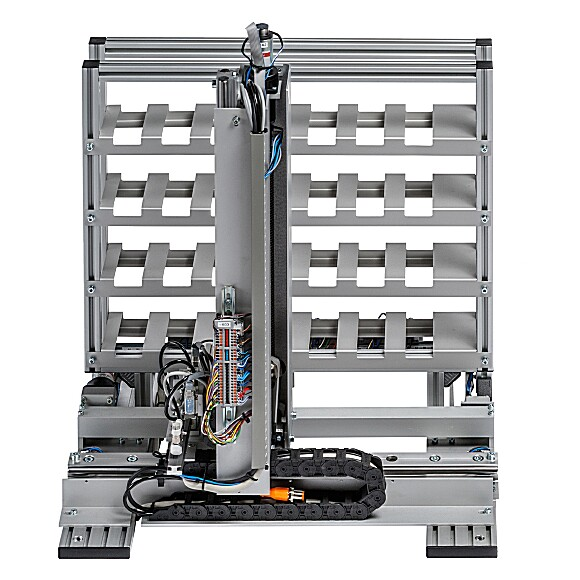
\includegraphics[width=8cm]{maquete/elevador/69523_3.jpg}
    };
    % \draw[red,ultra thick,rounded corners] (0,0) rectangle (9.4,6.2);
    \begin{scope}[x={(image.south east)},y={(image.north west)}]
        % \draw[help lines,xstep=.1,ystep=.1] (0,0) grid (1,1);
        % \foreach \x in {0,1,...,9} { \node [anchor=north] at (\x/10,0) {0.\x}; }
        % \foreach \y in {0,1,...,9} { \node [anchor=east] at (0,\y/10) {0.\y}; }
      \draw[red] (1,0.5) node {\textbf{Right}};
      \draw[red] (0,0.5) node {\textbf{Left}};
      \draw[red] (0.5,1) node {\textbf{Top}};
      \draw[red] (0.5,0) node {\textbf{Bottom}};
      \end{scope}
  \end{tikzpicture}
  \caption{Storage Unit}
\end{figure}


\begin{figure}[H]
  \centering
  \begin{tikzpicture}
    \node[anchor=south west,inner sep=0] (image) at (0,0) {
      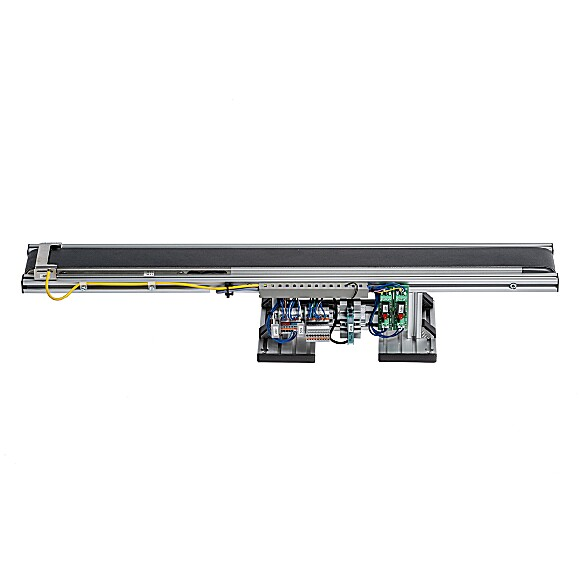
\includegraphics[trim={0 6cm 0 5cm},clip,width=8cm]{maquete/esteira/40778_3.jpg}
    };
    % \draw[red,ultra thick,rounded corners] (0,0) rectangle (9.4,6.2);
    \begin{scope}[x={(image.south east)},y={(image.north west)}]
        % \draw[help lines,xstep=.1,ystep=.1] (0,0) grid (1,1);
        % \foreach \x in {0,1,...,9} { \node [anchor=north] at (\x/10,0) {0.\x}; }
        % \foreach \y in {0,1,...,9} { \node [anchor=east] at (0,\y/10) {0.\y}; }
        \draw [->,>=stealth,red, very thick](0.9,0.7) -- (0.1,0.7);
        \draw [red] (0.5,0.8) node {Forward};
        \draw [->,>=stealth,red, very thick](0.1,0.1) -- (0.9,0.1);
        \draw [red](0.5,0.0) node {Reverse};
      \end{scope}
  \end{tikzpicture}
  \caption{Conveyor Belt}
\end{figure}

\begin{figure}[H]
  \centering
  \begin{tikzpicture}
    \node[anchor=south west,inner sep=0] (image) at (0,0) {
      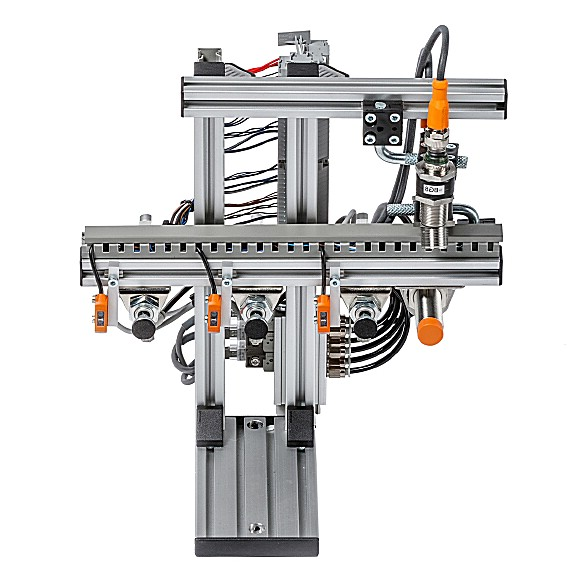
\includegraphics[trim={0 0 0 0},clip,width=8cm]{maquete/sensores/69511_3.jpg}
    };
    % \draw[red,ultra thick,rounded corners] (0,0) rectangle (9.4,6.2);
    \begin{scope}[x={(image.south east)},y={(image.north west)}]
        % \draw[help lines,xstep=.1,ystep=.1] (0,0) grid (1,1);
        % \foreach \x in {0,1,...,9} { \node [anchor=north] at (\x/10,0) {0.\x}; }
        % \foreach \y in {0,1,...,9} { \node [anchor=east] at (0,\y/10) {0.\y};  }
        \draw[red,ultra thick,rounded corners] (0.15,0.4) rectangle ++ (0.15,0.1);
        \draw[red] (0.1,0.1) node {\textbf{Left}};
        \draw[->,>=stealth,red, very thick] (0.2,0.38) -- (0.1,0.15);
        \draw[magenta,ultra thick,rounded corners] (0.35,0.4) rectangle ++ (0.15,0.1);
        \draw[magenta] (0.1,0.8) node {\textbf{Center}};
        \draw[->,>=stealth,magenta, very thick] (0.4,0.52) -- (0.2,0.75);
        \draw[cyan,ultra thick,rounded corners] (0.53,0.4) rectangle ++ (0.15,0.1);
        \draw[cyan] (0.7,0.1) node {\textbf{Right}};
        \draw[->,>=stealth,cyan, very thick] (0.65,0.38) -- (0.7,0.15);
      \end{scope}
  \end{tikzpicture}
  \caption{Sensors}
\end{figure}

\begin{figure}[H]
  \centering
  \begin{tikzpicture}
    \node[anchor=south west,inner sep=0] (image) at (0,0) {
      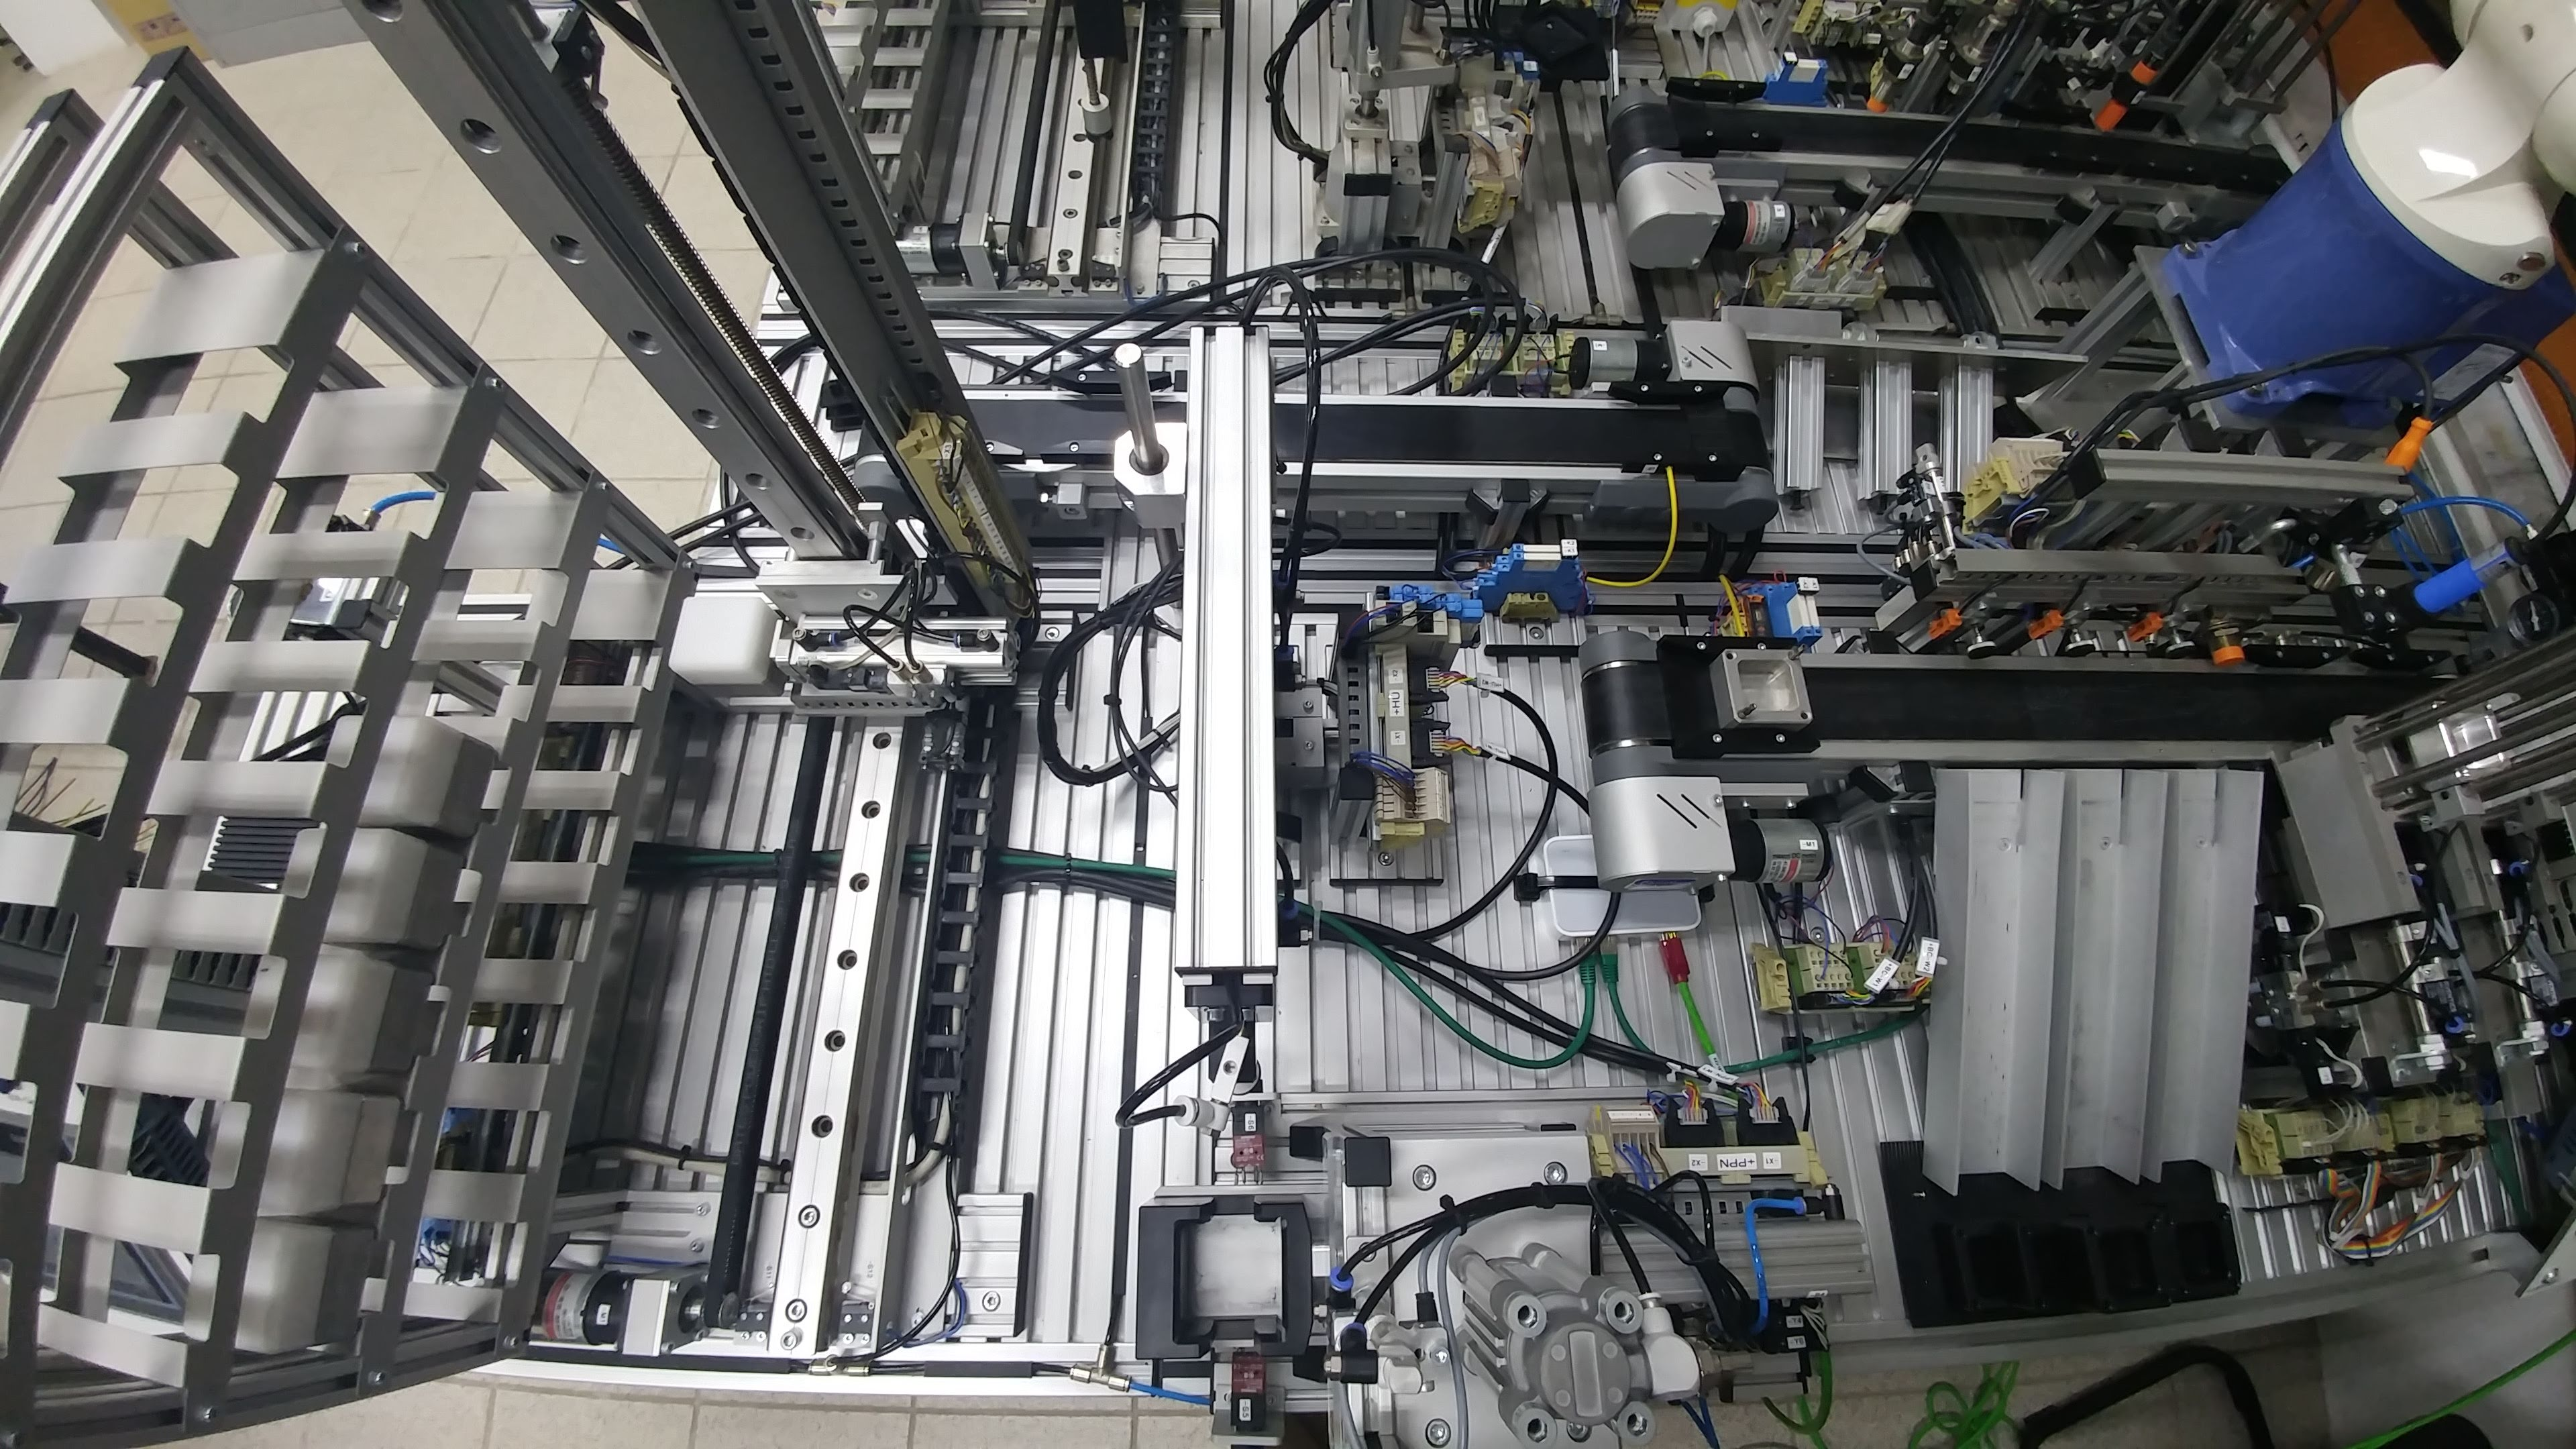
\includegraphics[trim={20cm 0 30cm 20cm},clip,width=0.8\textwidth]{maquete/armAngles.jpg}
    };
    % \draw[red,ultra thick,rounded corners] (0,0) rectangle (9.4,6.2);
    \begin{scope}[x={(image.south east)},y={(image.north west)}]
        % \draw[help lines,xstep=.1,ystep=.1] (0,0) grid (1,1);
        % \foreach \x in {0,1,...,9} { \node [anchor=north] at (\x/10,0) {0.\x}; }
        % \foreach \y in {0,1,...,9} { \node [anchor=east] at (0,\y/10) {0.\y}; }a
        
      
        \draw[red,->,>=stealth,very thick] (0.48,0.9) -- ++(-50:0.7);
        \draw[red,->,>=stealth,very thick] (0.48,0.9) -- ++(-95:0.7);
        \draw[red,->,>=stealth,very thick] (0.48,0.9) -- ++(-120:0.7);

        \draw[fill=red, fill opacity=0.2,draw=none] (0.48,0.9) -- ([shift=(-50:0.5)]0.48,0.9) arc (-50:-95:0.5);
        \draw[fill=blue, fill opacity=0.2,draw=none] (0.48,0.9) -- ([shift=(-95:0.5)]0.48,0.9) arc (-95:-120:0.5);

        \draw [fill,white,fill opacity=0.7,draw=none] (0.02,0.23) rectangle ++ (0.35,0.06);
        \draw [black] (0.2,0.25) node {\tiny \textbf{STORAGE\_ANGLE\_BEFORE}};

        \draw [fill,white,fill opacity=0.7,draw=none] (0.25,0.13) rectangle ++ (0.3,0.06);
        \draw [black] (0.4,0.15) node {\tiny \textbf{PRESS\_ANGLE\_AFTER}};

        \draw [fill,white,fill opacity=0.7,draw=none] (0.7,0.28) rectangle ++ (0.3,0.06);
        \draw [black] (0.85,0.3) node {\tiny \textbf{PRESS\_ANGLE\_BEFORE}};

        \draw [fill,white,fill opacity=0.7,draw=none] (0.1,0.82) rectangle  (0.2,0.96);
        \draw [red,thick] ([shift=(0:0.03)]0.15,0.9) arc (0:180:0.03);
        \draw[black,->,>=stealth,very thick] (0.15,0.85) -- ++(0,0.1);
        \draw [red,->,>=stealth,thick] ([shift=(0:-0.03)]0.15,0.9) arc (-180:-20:0.03);

      \end{scope}
  \end{tikzpicture}
  \caption{Sensors}
\end{figure}

Identification algorithm as seen in \cite{moreira2018enhanced}
\begin{algorithm2e}
  \caption{Identification Algorithm}\label{alg:identification}
\KwIn
{%
Modified observed paths $p_i^k$, for i= 1,\dots,$r$
}
\KwOut
{%
DAOCT = $($\XSet,\SigmaSet,\OmegaSet,\ffunction,\lambdafunction,\RSet,\thetafunction,\xZero,\XfSet$)$
}
\BlankLine
Create an initial state $x_0$, and define $\lambda(x_0) = \tilde{\lambda}(x_0) =
y_{1,1}$

$X = \{ x_0\}, X_f = \emptyset$

\For{$i = 1$ \KwTo $r$}
{
\For{$j = 1$ \KwTo $l_i - 1$}
{
  Find the State $x \in X $ such that $\tilde{\lambda}(x) = y_{i,j+1}$

  \eIf{$\tilde{\lambda}(x) \neq y_{i,j+1}$ for all $ x \in X$}
  { Create state $x^\prime$ and define $\tilde{\lambda}(x^\prime) = y_{i,j+1}$

$X = X \cup \{ x^\prime\}$

$\lambda(x^\prime) = \tilde{\lambda_l}(x^\prime)$

}
{
  Find $x^\prime \in X$ such that $\tilde{\lambda}(x^\prime) = y_{i,j+1}$
}
$f(x,\sigma_{i,j}) = x^\prime$

Add $i$ to $\theta(x,\sigma_{i,j})$

\If{$j = l_i - 1$}
{
  $X_f = X_f \cup \{x^\prime\}$
}
}
}
\end{algorithm2e}

% \begin{table}[H]
%   \centering
%   \caption{table}
%   \begin{tabular}{cc}
%     \label{tab:tab1}
%     \hypertarget{tab:1}{}
%     Transição&Significado\\
%     \hline \\
%     \hyperlink{partialNet:t1}{\hypertarget{partialTable:t1}{$t_{1}$}}&Test\\
%     \hyperlink{partialNet:p1}{\hypertarget{partialTable:p1}{$p_{1}$}}&balbalbal\\
%     \hyperlink{partialNet:p0m2}{\hypertarget{partialTable:p0m2}{$p_{0}$}}&balbalbal
%   \end{tabular}
% \end{table}

% \newpage
% \begin{figure}[h]
%   \centering
%   \begin{tikzpicture}[>=latex',line join=bevel,]
%%
\node (p0m2) at (27.0bp,18.0bp) [draw,ellipse,place, tokens=2, label=above:, label=left:\hyperlink{partialTable:p0m2}{\hypertarget{partialNet:p0m2}{$p_{0}$}},rotate=90] {};
  \node (tt1) at (114.0bp,18.0bp) [draw,ellipse,timedtransition, label=above:, label=left:\hyperlink{partialTable:tt1}{\hypertarget{partialNet:tt1}{$t_{1}$}},rotate=90] {};
  \node (ep1) at (185.0bp,18.0bp) [draw,ellipse,extPlace, label=above:, label=left:\hyperlink{partialNet:p1}{$p_{1}$},rotate=90] {};
  \draw [-Latex,inhibitor] (p0m2) ..controls (54.05bp,18.0bp) and (76.966bp,18.0bp)  .. (tt1);
  \definecolor{strokecol}{rgb}{0.0,0.0,0.0};
  \pgfsetstrokecolor{strokecol}
  \draw (70.5bp,27.0bp) node {3};
  \draw [-Latex] (tt1) ..controls (141.25bp,18.0bp) and (147.94bp,18.0bp)  .. (ep1);
%
\end{tikzpicture}

%   \caption{example }
%   \label{fig:example}
% \end{figure}

% \newpage
% \begin{figure}[h]
%   \centering
%   \begin{tikzpicture}[>=latex',line join=bevel,]
%%
\node (et1) at (27.0bp,18.0bp) [draw,ellipse,extTransition, label=above:, label=left:\hyperlink{partialNet:t1}{$t_{1}$},rotate=90] {};
  \node (p1) at (95.0bp,18.0bp) [draw,ellipse,place, label=above:, label=left:\hyperlink{partialTable:p1}{\hypertarget{partialNet:p1}{$p_{1}$}},rotate=90] {};
  \draw [-Latex] (et1) ..controls (54.266bp,18.0bp) and (57.727bp,18.0bp)  .. (p1);
%
\end{tikzpicture}

%   \caption{example }
%   \label{fig:example}
% \end{figure}

% \newpage

% \begin{figure}[H]
%   \centering
%   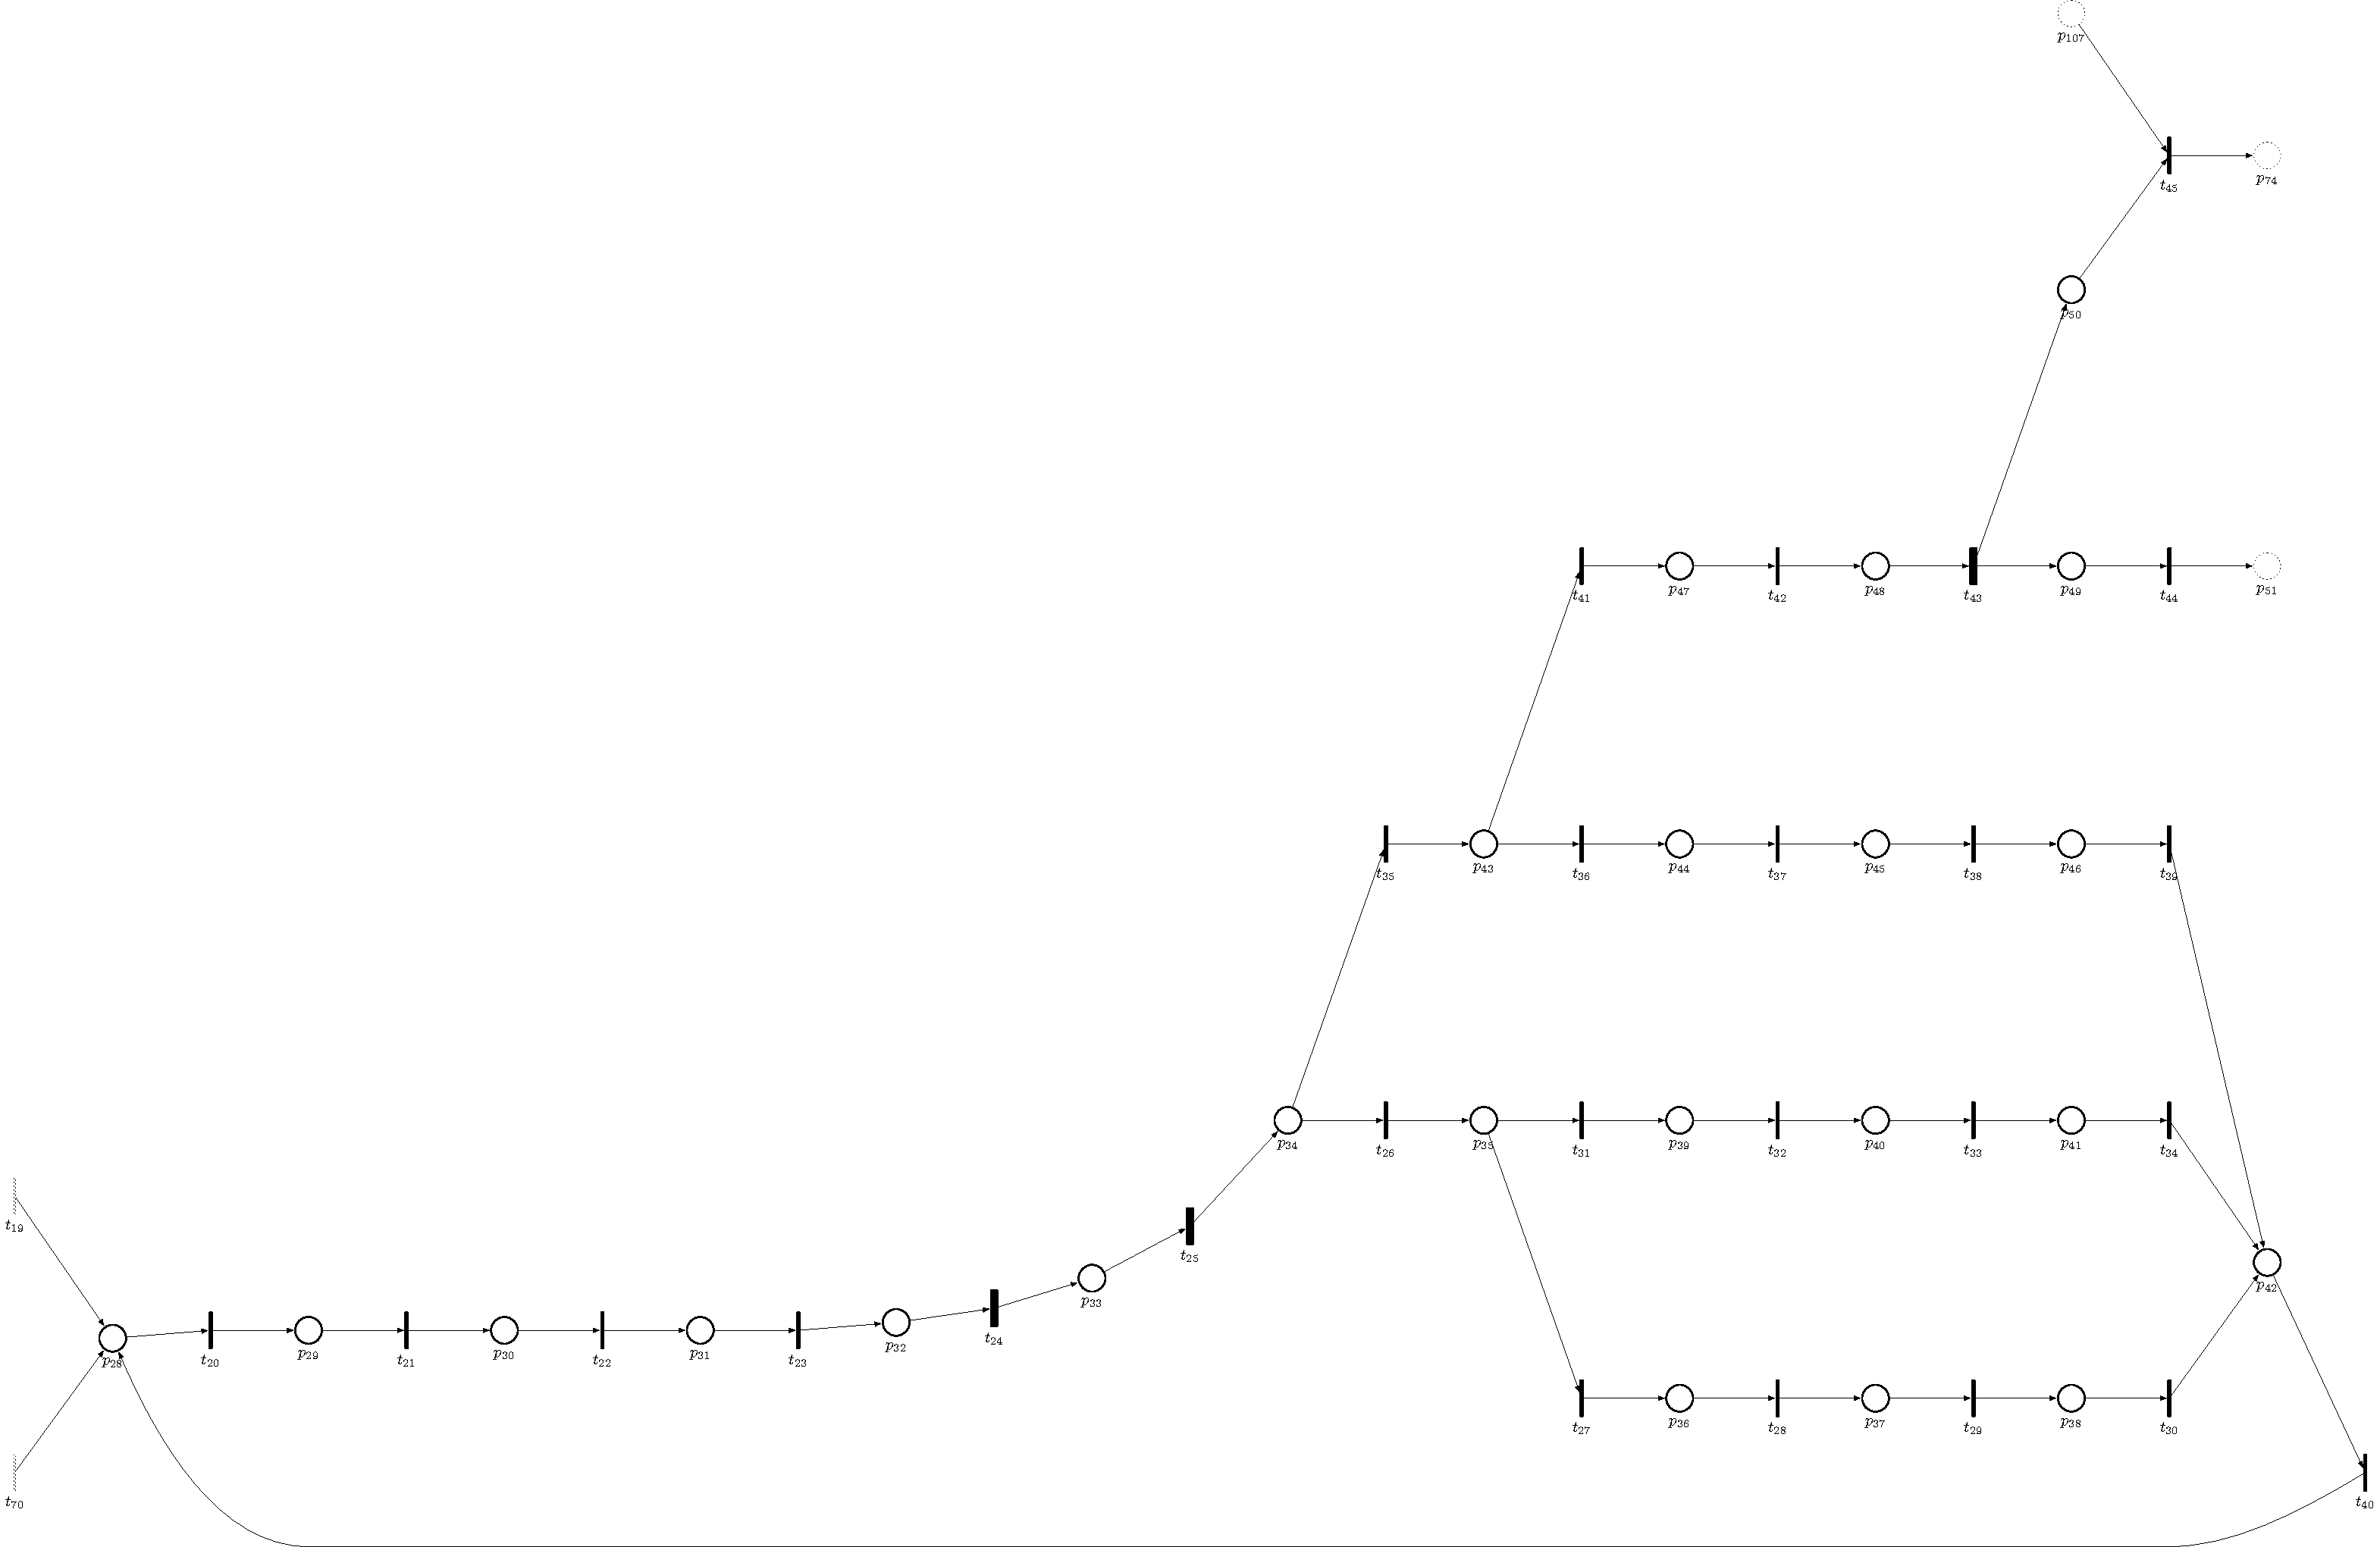
\includegraphics{../../figures/petriNet/dot/2-metalv/metalv.pdf}
%   \caption{qlksdjf}
%   \label{fig:example}
% \end{figure}


% \begin{figure}[H]
%   \centering
%   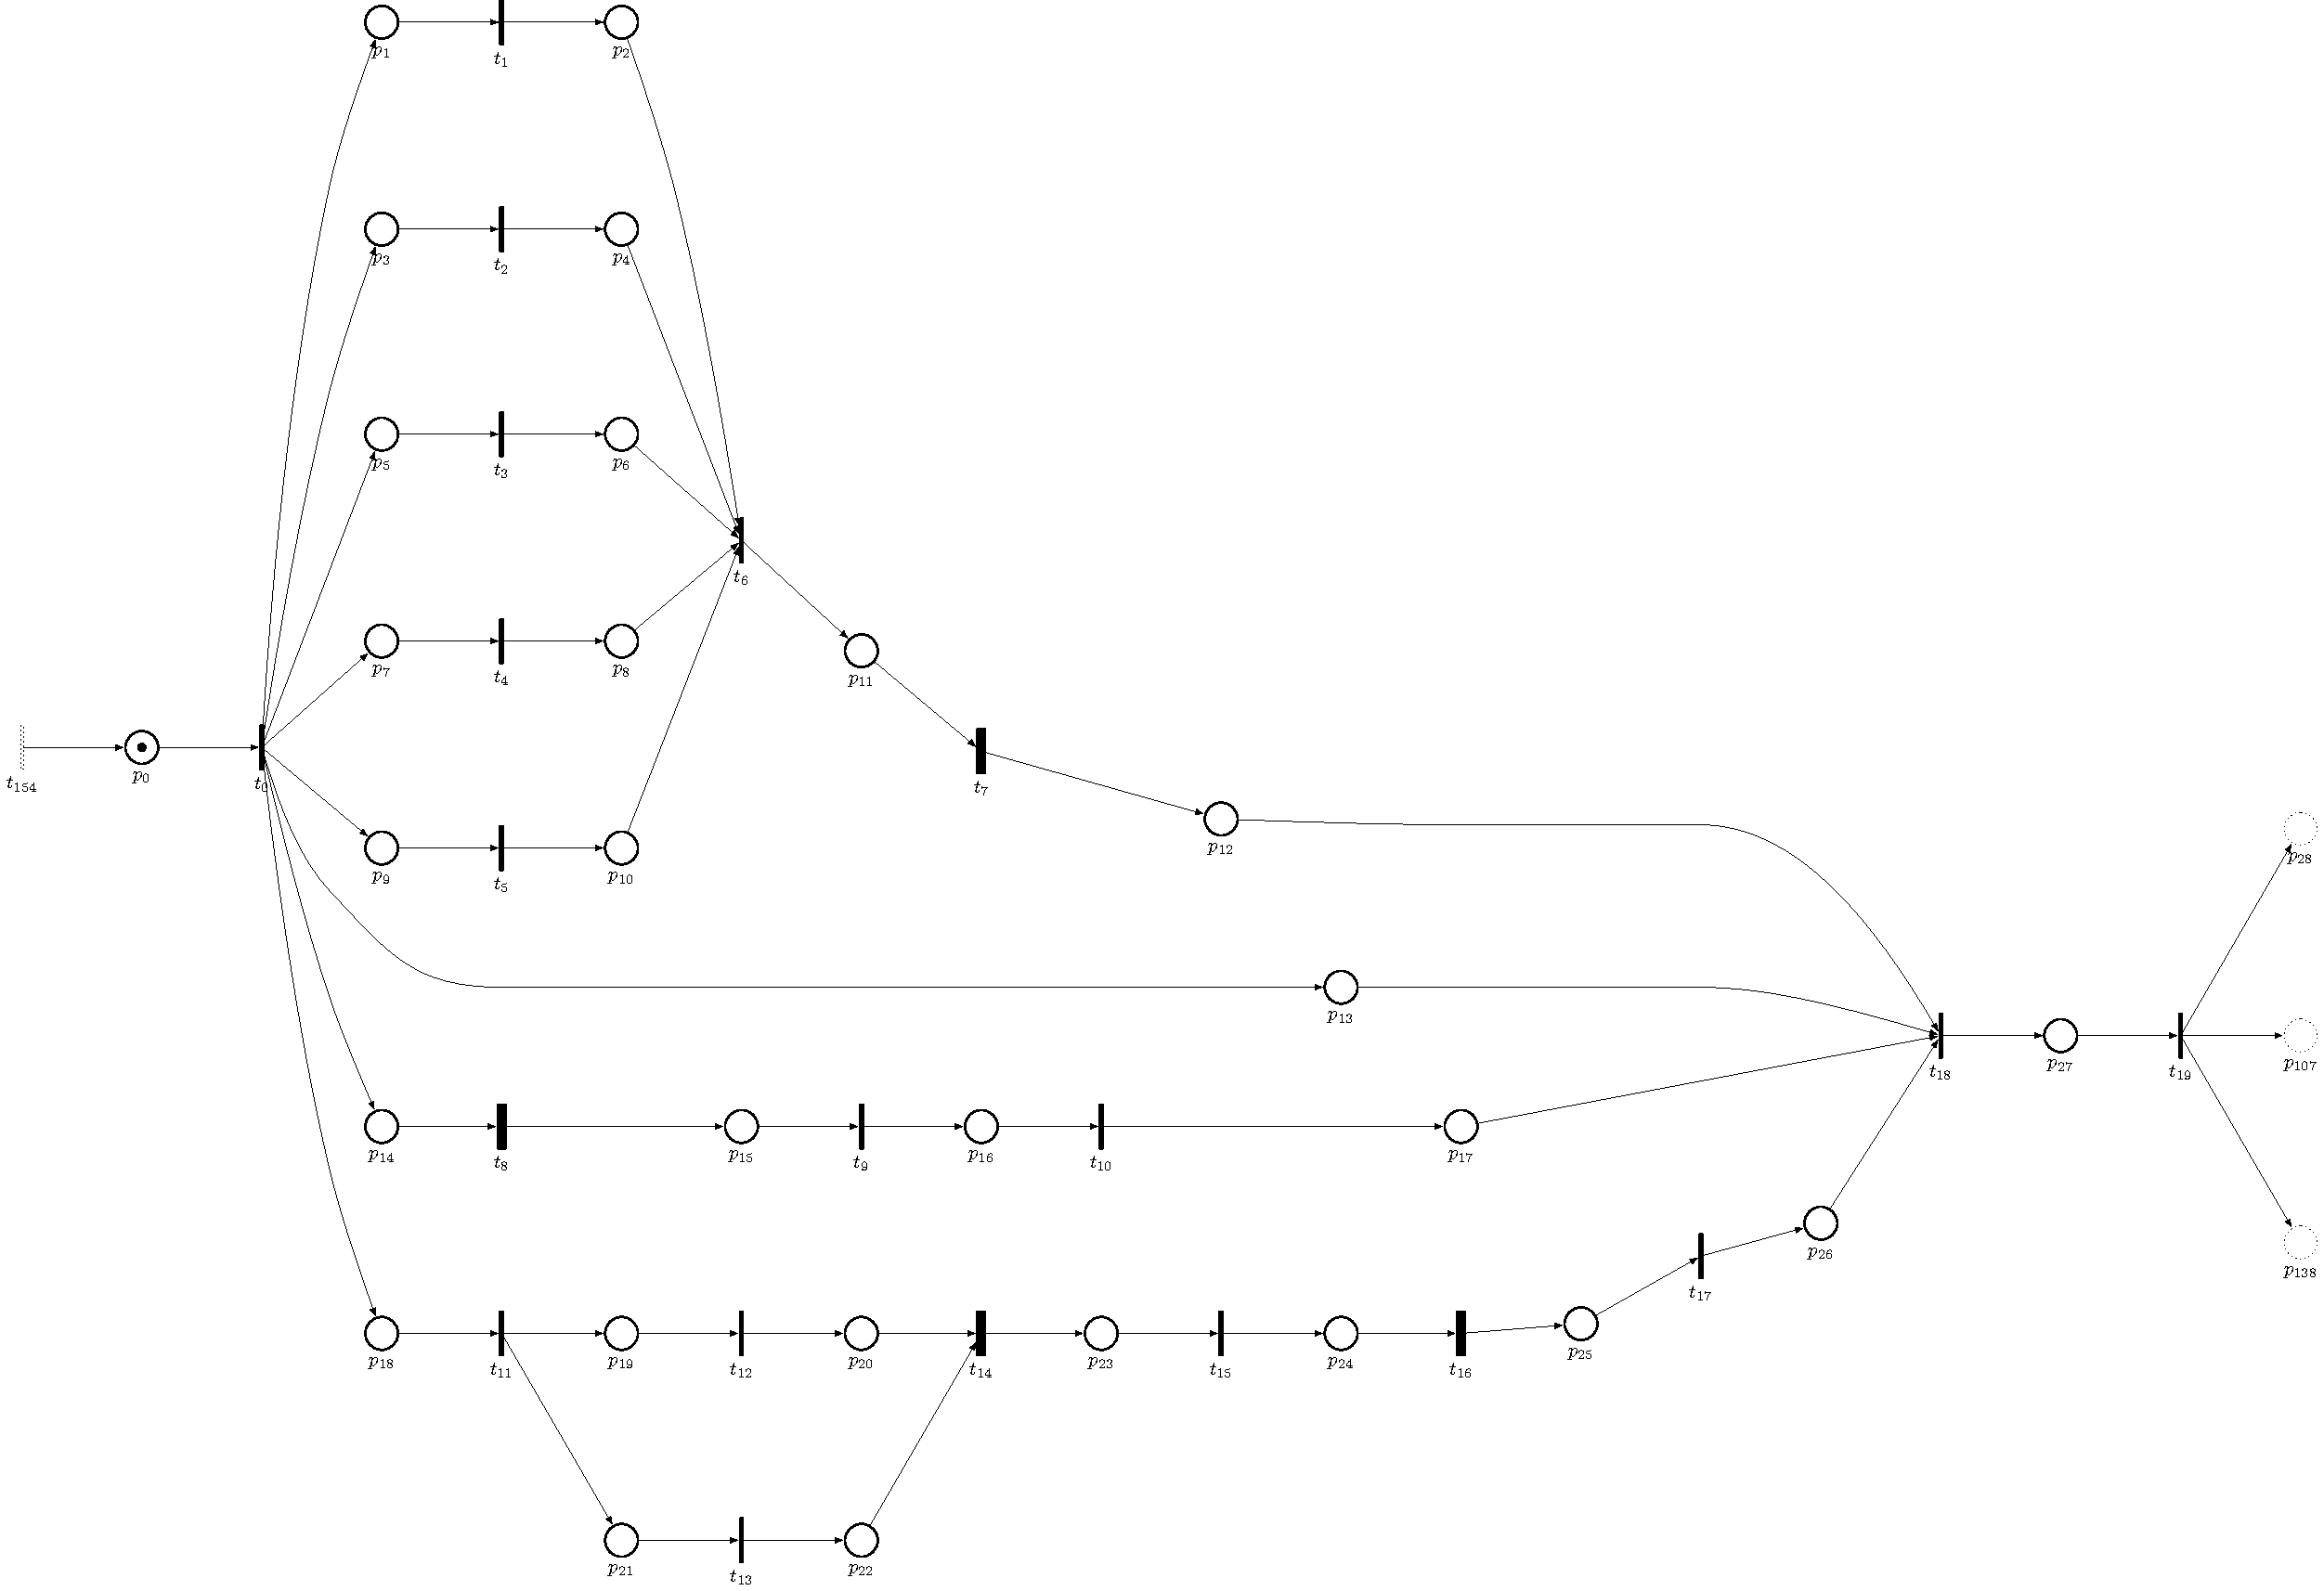
\includegraphics[width=0.4\textwidth]{../../figures/partial/initial.tikz}
%   \caption{petri net bal}
%   \label{fig:petrinetexample}
% \end{figure}

% \addtikzfigure{../../figures/petriNet/partial/initial}
% {Petri net of cube storage module.}
% {petri_initialization}

% \addtikzfigure{../../figures/petriNet//partial/metalv}
% {Petri net of metal cube half sorting module.}
% {petri_initialization}

\begin{table}[htbp]
\caption{Initialization Module Places.}
\centering
\begin{tabular}{M{5cm}M{10cm}}
Places & Meaning\\
\hline
\hyperlink{partialNet:p0m1}{\hypertarget{partialTable:p0m1}{$p_{0}$}} & System Stopped\\
\hyperlink{partialNet:p1}{\hypertarget{partialTable:p1}{$p_{1}$}} & Retract MAG1's Cylinder *\\
\hyperlink{partialNet:p2}{\hypertarget{partialTable:p2}{$p_{2}$}} & MAG1's Cylinder Retracted\\
\hyperlink{partialNet:p3}{\hypertarget{partialTable:p3}{$p_{3}$}} & Retract MAG2's Cylinder *\\
\hyperlink{partialNet:p4}{\hypertarget{partialTable:p4}{$p_{4}$}} & MAG2's Cylinder Retracted\\
\hyperlink{partialNet:p5}{\hypertarget{partialTable:p5}{$p_{5}$}} & Retract Right Discharge Cylinder *\\
\hyperlink{partialNet:p6}{\hypertarget{partialTable:p6}{$p_{6}$}} & Right Discharge Cylinder Retracted\\
\hyperlink{partialNet:p7}{\hypertarget{partialTable:p7}{$p_{7}$}} & Retract Center Discharge Cylinder\\
\hyperlink{partialNet:p8}{\hypertarget{partialTable:p8}{$p_{8}$}} & Center Discharge Cylinder Retracted\\
\hyperlink{partialNet:p9}{\hypertarget{partialTable:p9}{$p_{9}$}} & Retract Left Discharge Cylinder *\\
\hyperlink{partialNet:p10}{\hypertarget{partialTable:p10}{$p_{10}$}} & Left Discharge Cylinder Retracted\\
\hyperlink{partialNet:p11}{\hypertarget{partialTable:p11}{$p_{11}$}} & Turn Conveyor Belt On (Reverse)\\
\hyperlink{partialNet:p12}{\hypertarget{partialTable:p12}{$p_{12}$}} & No Pieces On Conveyor Belt\\
\hyperlink{partialNet:p13}{\hypertarget{partialTable:p13}{$p_{13}$}} & Reset Variables\\
\hyperlink{partialNet:p14}{\hypertarget{partialTable:p14}{$p_{14}$}} & Raise Press\\
\hyperlink{partialNet:p15}{\hypertarget{partialTable:p15}{$p_{15}$}} & Open Safety Door\\
\hyperlink{partialNet:p16}{\hypertarget{partialTable:p16}{$p_{16}$}} & Extend Assembly Unit Holder\\
\hyperlink{partialNet:p17}{\hypertarget{partialTable:p17}{$p_{17}$}} & Assembly Unit Ready\\
\hyperlink{partialNet:p18}{\hypertarget{partialTable:p18}{$p_{18}$}} & Arm Lowered and Retracted, and Storage Unit Retracted\\
\hyperlink{partialNet:p19}{\hypertarget{partialTable:p19}{$p_{19}$}} & Move Storage Unit to the Right\\
\hyperlink{partialNet:p20}{\hypertarget{partialTable:p20}{$p_{20}$}} & Storage Unit ready ( horizontal )\\
\hyperlink{partialNet:p21}{\hypertarget{partialTable:p21}{$p_{21}$}} & Move Storage Device Downwards\\
\hyperlink{partialNet:p22}{\hypertarget{partialTable:p22}{$p_{22}$}} & Storage Unit ready ( vertical )\\
\hyperlink{partialNet:p23}{\hypertarget{partialTable:p23}{$p_{23}$}} & Rotate Arm CCW\\
\hyperlink{partialNet:p24}{\hypertarget{partialTable:p24}{$p_{24}$}} & Turn HSC Off ( Arm Stopped )\\
\hyperlink{partialNet:p25}{\hypertarget{partialTable:p25}{$p_{25}$}} & Rotate Arm CW\\
\hyperlink{partialNet:p26}{\hypertarget{partialTable:p26}{$p_{26}$}} & Arm Stopped facing conveyor belt\\
\hyperlink{partialNet:p27}{\hypertarget{partialTable:p27}{$p_{27}$}} & System Ready\\
\end{tabular}
\end{table}


\begin{table}[H]
\caption{Initialization Module Transitions.}
\centering
\begin{tabular}{M{5cm}M{10cm}}
Transitions & Meaning\\
\hline
\hyperlink{partialNet:t0}{\hypertarget{partialTable:t0}{$t_{0}$}} & Initialization Button\\
\hyperlink{partialNet:t1}{\hypertarget{partialTable:t1}{$t_{1}$}} & MAG1's Cylinder Retracted\\
\hyperlink{partialNet:t2}{\hypertarget{partialTable:t2}{$t_{2}$}} & MAG2's Cylinder Retracted\\
\hyperlink{partialNet:t3}{\hypertarget{partialTable:t3}{$t_{3}$}} & Right Discharge Cylinder Retracted\\
\hyperlink{partialNet:t4}{\hypertarget{partialTable:t4}{$t_{4}$}} & Center Discharge Cylinder Retracted\\
\hyperlink{partialNet:t5}{\hypertarget{partialTable:t5}{$t_{5}$}} & Left Discharge Cylinder Retracted\\
\hyperlink{partialNet:t6}{\hypertarget{partialTable:t6}{$t_{6}$}} & \\
\hyperlink{partialNet:tt7}{\hypertarget{partialTable:tt7}{$t_{7}$}} & T=12s\\
\hyperlink{partialNet:tt8}{\hypertarget{partialTable:tt8}{$t_{8}$}} & T=2.5s\\
\hyperlink{partialNet:t9}{\hypertarget{partialTable:t9}{$t_{9}$}} & Safety Door Opened\\
\hyperlink{partialNet:t10}{\hypertarget{partialTable:t10}{$t_{10}$}} & Assembly Unit Holder Extended\\
\hyperlink{partialNet:t11}{\hypertarget{partialTable:t11}{$t_{11}$}} & Storage Unit Retracted and Arm Lowered and Retracted\\
\hyperlink{partialNet:t12}{\hypertarget{partialTable:t12}{$t_{12}$}} & Storage Unit Right Limit Switch\\
\hyperlink{partialNet:t13}{\hypertarget{partialTable:t13}{$t_{13}$}} & Storage Unit Inferior Limit Switch\\
\hyperlink{partialNet:tt14}{\hypertarget{partialTable:tt14}{$t_{14}$}} & T=2s\\
\hyperlink{partialNet:t15}{\hypertarget{partialTable:t15}{$t_{15}$}} & Inductive Sensor Arm\\
\hyperlink{partialNet:tt16}{\hypertarget{partialTable:tt16}{$t_{16}$}} & T=1s\\
\hyperlink{partialNet:t17}{\hypertarget{partialTable:t17}{$t_{17}$}} & ARMCOUNTER <= BELT\_ANGLE\_CW\\
\hyperlink{partialNet:t18}{\hypertarget{partialTable:t18}{$t_{18}$}} & \\
\hyperlink{partialNet:t19}{\hypertarget{partialTable:t19}{$t_{19}$}} & Start Button\\
\end{tabular}
\end{table}


\begin{longtable}{M{5cm}M{10cm}}
\caption{Metal Half-cube Selection Module Places.} \label{tab:metalvPlaces}
\\
Places & Meaning\\
\hline
\endfirsthead
\multicolumn{2}{l}{Continued from previous page} \\
\hline

Places & Meaning \\

\hline
\endhead
\hline\multicolumn{2}{r}{Continued on next page} \\
\endfoot
\endlastfoot
\hline
\hyperlink{partialNet:p28}{\hypertarget{partialTable:p28}{$p_{28}$}} & MAG1 Empty\\
\hyperlink{partialNet:p29}{\hypertarget{partialTable:p29}{$p_{29}$}} & MAG1 Not Empty\\
\hyperlink{partialNet:p30}{\hypertarget{partialTable:p30}{$p_{30}$}} & Extend MAG1's Cylinder *\\
\hyperlink{partialNet:p31}{\hypertarget{partialTable:p31}{$p_{31}$}} & Retract MAG1's Cylinder *\\
\hyperlink{partialNet:p32}{\hypertarget{partialTable:p32}{$p_{32}$}} & MAG1's Cylinder Retracted\\
\hyperlink{partialNet:p33}{\hypertarget{partialTable:p33}{$p_{33}$}} & Turn Conveyor Belt On\\
\hyperlink{partialNet:p34}{\hypertarget{partialTable:p34}{$p_{34}$}} & \\
\hyperlink{partialNet:p35}{\hypertarget{partialTable:p35}{$p_{35}$}} & Plastic Half-cube\\
\hyperlink{partialNet:p36}{\hypertarget{partialTable:p36}{$p_{36}$}} & Turn Conveyor Belt On\\
\hyperlink{partialNet:p37}{\hypertarget{partialTable:p37}{$p_{37}$}} & Extend Right Discharge Cylinder *\\
\hyperlink{partialNet:p38}{\hypertarget{partialTable:p38}{$p_{38}$}} & Retract Right Discharge Cylinder *\\
\hyperlink{partialNet:p39}{\hypertarget{partialTable:p39}{$p_{39}$}} & Turn Conveyor Belt On\\
\hyperlink{partialNet:p40}{\hypertarget{partialTable:p40}{$p_{40}$}} & Extend Center Discharge Cylinder *\\
\hyperlink{partialNet:p41}{\hypertarget{partialTable:p41}{$p_{41}$}} & Retract Center Discharge Cylinder *\\
\hyperlink{partialNet:p42}{\hypertarget{partialTable:p42}{$p_{42}$}} & \\
\hyperlink{partialNet:p43}{\hypertarget{partialTable:p43}{$p_{43}$}} & Metal Half-cube\\
\hyperlink{partialNet:p44}{\hypertarget{partialTable:p44}{$p_{44}$}} & Turn Conveyor Belt On\\
\hyperlink{partialNet:p45}{\hypertarget{partialTable:p45}{$p_{45}$}} & Extend Left Discharge Cylinder *\\
\hyperlink{partialNet:p46}{\hypertarget{partialTable:p46}{$p_{46}$}} & Retract Left Discharge Cylinder *\\
\hyperlink{partialNet:p47}{\hypertarget{partialTable:p47}{$p_{47}$}} & Turn Conveyor Belt On\\
\hyperlink{partialNet:p48}{\hypertarget{partialTable:p48}{$p_{48}$}} & Turn Conveyor Belt On\\
\hyperlink{partialNet:p49}{\hypertarget{partialTable:p49}{$p_{49}$}} & Metal Half-cube Ready\\
\hyperlink{partialNet:p50}{\hypertarget{partialTable:p50}{$p_{50}$}} & Conveyor Belt Stopped\\
\end{longtable}


\begin{table}[H]
\caption{Metal Half-cube Selection Module Transitions.}
\centering
\begin{tabular}{M{5cm}M{10cm}}
Transitions & Meaning\\
\hline
\hyperlink{partialNet:t20}{\hypertarget{partialTable:t20}{$t_{20}$}} & \(\overline{\mbox{MAG1 Empty}}\)\\
\hyperlink{partialNet:t21}{\hypertarget{partialTable:t21}{$t_{21}$}} & \\
\hyperlink{partialNet:t22}{\hypertarget{partialTable:t22}{$t_{22}$}} & MAG1's Cylinder Extended \(\uparrow\)\\
\hyperlink{partialNet:t23}{\hypertarget{partialTable:t23}{$t_{23}$}} & MAG1's Cylinder Retracted \(\uparrow\)\\
\hyperlink{partialNet:tt24}{\hypertarget{partialTable:tt24}{$t_{24}$}} & T=0.5s\\
\hyperlink{partialNet:tt25}{\hypertarget{partialTable:tt25}{$t_{25}$}} & Presence \(\uparrow\) T=0.5s\\
\hyperlink{partialNet:t26}{\hypertarget{partialTable:t26}{$t_{26}$}} & \(\overline{\mbox{Metallic Sensor}}\)\\
\hyperlink{partialNet:t27}{\hypertarget{partialTable:t27}{$t_{27}$}} & \(\overline{\mbox{White Color Sensor}}\)\\
\hyperlink{partialNet:t28}{\hypertarget{partialTable:t28}{$t_{28}$}} & Proximity Sensor Left Discharge Cylinder \(\uparrow\)\\
\hyperlink{partialNet:t29}{\hypertarget{partialTable:t29}{$t_{29}$}} & Right Discharge Cylinder Extended\\
\hyperlink{partialNet:t30}{\hypertarget{partialTable:t30}{$t_{30}$}} & Right Discharge Cylinder Retracted\\
\hyperlink{partialNet:t31}{\hypertarget{partialTable:t31}{$t_{31}$}} & White Color Sensor\\
\hyperlink{partialNet:t32}{\hypertarget{partialTable:t32}{$t_{32}$}} & Proximity Sensor Center Discharge Cylinder \(\uparrow\)\\
\hyperlink{partialNet:t33}{\hypertarget{partialTable:t33}{$t_{33}$}} & Center Discharge Cylinder Extended\\
\hyperlink{partialNet:t34}{\hypertarget{partialTable:t34}{$t_{34}$}} & Center Discharge Cylinder Retracted\\
\hyperlink{partialNet:t35}{\hypertarget{partialTable:t35}{$t_{35}$}} & Metallic Sensor\\
\hyperlink{partialNet:t36}{\hypertarget{partialTable:t36}{$t_{36}$}} & Concavity Downwards\\
\hyperlink{partialNet:t37}{\hypertarget{partialTable:t37}{$t_{37}$}} & Proximity Sensor Left Discharge Cylinder \(\uparrow\)\\
\hyperlink{partialNet:t38}{\hypertarget{partialTable:t38}{$t_{38}$}} & Left Discharge Cylinder Extended\\
\hyperlink{partialNet:t39}{\hypertarget{partialTable:t39}{$t_{39}$}} & Left Discharge Cylinder Retracted\\
\hyperlink{partialNet:t40}{\hypertarget{partialTable:t40}{$t_{40}$}} & \\
\hyperlink{partialNet:t41}{\hypertarget{partialTable:t41}{$t_{41}$}} & Concavity Upwards\\
\hyperlink{partialNet:t42}{\hypertarget{partialTable:t42}{$t_{42}$}} & Proximity Sensor End Of Conveyor Belt \(\uparrow\)\\
\hyperlink{partialNet:tt43}{\hypertarget{partialTable:tt43}{$t_{43}$}} & T=0.5s\\
\hyperlink{partialNet:t44}{\hypertarget{partialTable:t44}{$t_{44}$}} & Proximity Sensor End Of Conveyor Belt \(\downarrow\)\\
\hyperlink{partialNet:t45}{\hypertarget{partialTable:t45}{$t_{45}$}} & \\
\end{tabular}
\end{table}


%%% Local Variables:
%%% mode: latex
%%% TeX-master: "../monografia"
%%% End:



\chapter{Introduction}
In a world where the majority of the population lives in industrial societies,
and machines take part on the bulk of the production of almost all goods: from
food to cosmetics and drugs, from toothbrushes to automobiles, 
a well-paced throughput it is crucial, and any non expected halt on the
production or change can be disastrous, producing sometimes multimillionaire debts,
provoking a snowball effect, affecting the economy and consequentially the welfare of the society.

A diverse number of causes of the halt or change of the throughput can be
accounted for. Some are as simple as a power outage, or a component malfunction,
but nowadays there are other players. As the industry \textsl{walks}, or even
better \textsl{runs}, towards the so called Fourth Industrial Revolution, the industry
urges the use of \textit{connected sensors}, since the Internet of Things is the
fashion these days, but the concerns about cyber security are now and again neglected.   
So hackers can infiltrate the system, and depending of the infrastructure
halt or change somehow the production throughput.

Cyber security is not the theme of this thesis but its theme is another important concern to a
well-paced throughput, failure detection.

As great part of the manufacture facilities uses conveyor
belts, pneumatic cylinders and digital sensors, it is very common to see \PLCs



\PLC 




\acr{oi}{oi}{oi}
\oi





khe  the most simple as  In order to prevent these effects lots of 
\todo{ objetivo mostrar que o metodo pode funcionar 
com comportamento paraelo mostrar a escabilidade
}
\doing{the objective of this thesis is to show that the \DAOCT model works with
  systems that presents parallel behavior dividing themand can be used to scalability }
\section{Thesis Outline}
\label{sec:thesisOutline}






%%% Local Variables:
%%% mode: latex
%%% TeX-master: "../monografia.tex"
%%% End:


\chapter{Background}
\label{cha:background}
This chapter will discuss the main topics needed to understand this work, from
discrete event systems to discrete control implementation on \PLCs, a more
detailed explanation of each topic can be found on the respective cited work.
\section{Systems}

A System as defined by the Cambridge's dictionary is ``a set of connected things
or devices that operate together''. As seen two basic properties of systems are
:
\begin{itemize}
\item they are formed by grouping smaller parts
\item the smaller parts when grouped work together to carry out a specific
  function
\end{itemize}

As its definition is so abstract almost anything can be defined as a system,
physical or not, beings can be defined as systems and even economic mechanisms
can also be considered as systems.

Usually systems are modelled by a Input\slash Output process. The system is fed with a
set of inputs, it process the inputs resulting on the output set, as we can see
in \autoref{fig:ioProcModel}.

\begin{figure}[H]
  \centering
  \begin{tikzpicture}
    % \node[anchor=south west,inner sep=0] (image) at (0,0) {
    %   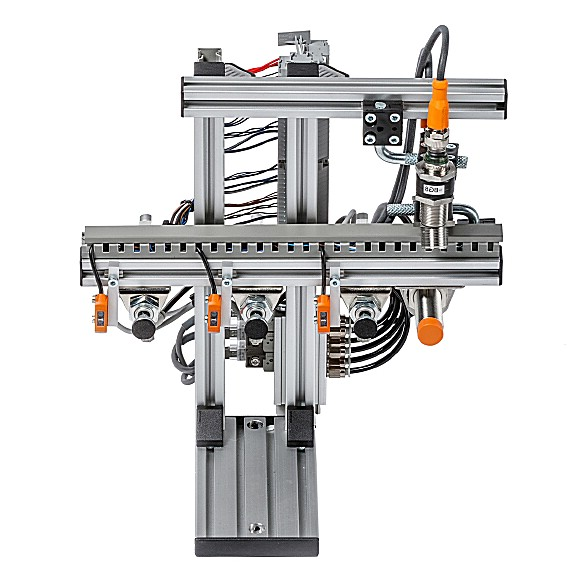
\includegraphics[trim={0 0 0 0},clip,width=8cm]{maquete/sensores/69511_3.jpg}
    % };
    % \draw[red,ultra thick,rounded corners] (0,0) rectangle (9.4,6.2);
    % \begin{scope}[x={(image.south east)},y={(image.north west)}]
        \draw[ultra thick,rounded corners] (3.5,4) rectangle (6.5,6);
        \draw (5,5) node {\textbf{Process}};
        \draw (0,5) node {\textbf{Inputs}};
        \draw[->,>=stealth, very thick] (1,4.5) -- ++ (2.5,0);
        \draw[->,>=stealth, very thick] (1,5)   -- ++ (2.5,0);
        \draw[->,>=stealth, very thick] (1,5.5) -- ++ (2.5,0);
        \draw (10,5) node {\textbf{Outputs}};
        \draw[->,>=stealth, very thick] (6.5,4.5) -- ++ (2.5,0);
        \draw[->,>=stealth, very thick] (6.5,5)   -- ++ (2.5,0);
        \draw[->,>=stealth, very thick] (6.5,5.5) -- ++ (2.5,0);
      % \end{scope}
    \end{tikzpicture}
  \caption{Input\slash Output Process model}
    \label{fig:ioProcModel}
\end{figure}


In some systems, its inputs and outputs can't represent it's behaviour, so the
concept of state is created, and it represents the behaviour of the system in a
given instant $t$.

The states can be continuous or discrete, and the systems which these states
represent can be considered as Continuous Systems, Discrete Systems or even
Hybrid Systems, which combine both kind of states.

The systems modelled in this work are Discrete Systems, more details about other
kinds of systems as well as examples and their analysis can be found on
\cite{oppenheim1996signals} and \cite{kalouptsidis1997signal}.
\section{Discrete Event Systems}
\label{sec:discreteEventSystems}
Discrete Systems can be driven by time and by events. It means, the states can
be changed continuously by the time or instantaneously by some ensemble of events.

In this thesis we are interested in the event-driven type. Some basic mathematical
formalisms, nomenclature and representations can be developed to facilitate the
understanding. Some of those will be presented in the following sections based
on \cite{cassandras2009introduction, david2005discrete,david1989grafcet}.
\section{Languages} \label{sec:automata} A language can be defined by the Merriam-Webster's dictionary as ``a systematic
means of communicating ideas or feelings by the use of conventionalized signs,
sounds, gestures, or marks having understood meanings'' And as it is defined by
this dictionary entry we pursue to communicate the complete behaviour of the
\DES. Firstly we need to define a group, or set of marks to characterise the
singular behaviour of the system. So, we define a set $\Sigma$. This set contains
all elements which combined can create a language. Again in analogy with
linguistics, each one of these marks, the events can be compared to letters ,
provided that $\Sigma$ can be called an ``alphabet'', and the combination of its
events ``words''. Words are also called ``strings '' or even ``traces''.
Considering the use of the word ``string'' as the variable type used on several
programming languages used in this work, we prefer the use of the vocables
``word'' and ``trace''. We can also define a mark to represent an empty word,
$\epsilon$, that is, a word that is not formed by any event.

The combination process to form words is called concatenation. For instance,
given two events $a$ and $b$, the words $ab$ and $ba$ can be created concatenating these two events and there is no particular reason to suppose that $ab$ is equal to $ba$, the same way the words ``ten'' and ``net'' have different meanings in English.

We can also concatenate two words, to create a different one, we can take the
words $ab$ and $ba$ and create words like $abba$ and $baab$.

As we extended the definition of concatenation to words, we define $\epsilon$,
the empty word, as the identity element of concatenation: $w\epsilon = \epsilon
w = w$ for any word $w$.

Likewise, we can define the length of a word as the number of events contained
by this word, we denote the length with two vertical bars, given a word $w$ its
length is equal to $|w|$ and by definition $|\epsilon| = 0 $.

As we know, there is a great number of human western languages, as portuguese,
english, french, spanish etc, that roughly are formed by the same alphabet, but
overall they are formed by different combination of words. Similar things can
happen with languages that define the \DESs, so we can define as in
\cite{cassandras2009introduction}.
% \pagebreak
\begin{definition}[Language]
  \label{def:language}~\\
  A Language defined over an alphabet $\Sigma$ is formed from finite-length
  words generated from the concatenation of the events in $\Sigma$ and
  $\epsilon$.
\end{definition}

Take for example an alphabet $\Sigma = \{a,b,g\}$, we can define different
languages
\begin{subequations}
  \begin{equation*}
  L_1=\{\epsilon, a, abb\}
  \end{equation*}
  \begin{equation*}
  L_2=\{\text{all possible words of length 3 starting with g}\}
  \end{equation*}
  \begin{equation*}
  L_3=\{\text{all possible words starting with g}\}
  \end{equation*}
\end{subequations}

The cardinality of this sets are $|L_1|=3$, $|L_2|=9$, $|L_3|=\infty$
As we can see from the same alphabet very different languages can be created, thus we can define a way to encapsulate all possible languages generated from
the same alphabet $\Sigma$. Let us denote by $\Sigma^*$ the set containing all
finite words composed with the elements of $\Sigma$ and $\epsilon$. The *
operation is called the \textit{Kleene-closure}. Similarly to $L_3$ it is
countably infinite since it contains arbitrarily long words. For instance the
\textit{Kleene-closure} of the alphabet $\Sigma = \{a, b, c\}$ is:
\begin{equation*}
  \label{eq:kleeneExample}
  \Sigma^* = \{\epsilon,a,b,c,aa,ab,ac,ba,bb,bc,ca,cb,cc,aaa,\dots\} 
\end{equation*}
There are a few operations with languages and alphabets that can be defined, but they are outside the scope of this work, they can be found on \cite{cassandras2009introduction}.
\section{Representation of Languages}
\label{sec:representationLanguages}

Although languages can describe the behaviour of \DESs, there are cases, as the
one shown
by the language $L_3$ in the last section, in which the language is enormous, in
that case countably infinite, what makes them not so simple to communicate the
behaviour of the system. For this purpose, there are some other formalisms that
aid the comprehension, since they can be a more compact way of expressing the
system's behaviour or accompanied by diagrams.

In the following subsections two of the most known representations will be
presented: Automata and Petri Nets.

% \pagebreak
\subsection{Automata}
\label{sec:automata}
One of the most known representation of languages are automata. The notion of
automaton is basically the definition of \DESs, as we saw in the
\autoref{sec:discreteEventSystems}: a set of events can change the state of the
system. If we know all the events composing the language of the
system and its states, we can have its alphabet $\Sigma$ and we can create a set $X$ composed
by all states.
From $\Sigma$ and $X$ we can derive a function that represents the transition
from a state to other, this function is called \emph{transition function} of the automaton
denoted as $f : X \times \Sigma \rightarrow X$. For example if a system have an
alphabet $\Sigma = \{a,b\}$ and 2 states, we can name the states $x$ and
$y$, and then create the set $X = \{x,y\}$. Knowing that the system begins at state $x$
and that when event $a$ happens it changes to state $z$ we can create a function
$f(x,a)$ and define it as $y$. Likewise if we know that when the system is at
state $y$ and event $b$ happens, a function $f(y,b)$ can be defined as $a$.

As a
visual aid, a representation of these functions can be made through a diagram, called \emph{state transition diagram}. In this kind of diagram the states are
represented by circles labeled with their names, and the functions as arcs
labeled with the corresponding event,connecting two states, with arrows in one of their
extremities indicating the transition from a state to other. The initial state
of the automaton has an arc pointing towards it coming from no other state.
\autoref{fig:functionDiagram} can represent the functions $f(x,a)$ and $f(y,b)$
described in the last paragraph.
\begin{figure}[H]
  \centering
  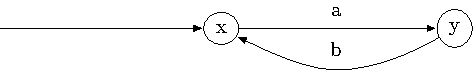
\includegraphics[width=0.3\textwidth]{automata/function/function.tikz}
  \caption{State Transition Diagram}
  \label{fig:functionDiagram}
\end{figure}
Now, for a more complex example, from \cite{cassandras2009introduction}:

\begin{example}[Simple Automaton] ~\\
  \label{ex:simpleAutomaton}
  Given $\Sigma = \{a,b,g\}$, $X = \{x,y,z\}$ and the following transition functions:
  \begin{align*}
   f(x,a)&=x&f(x,g)&=z\\
   f(y,a)&=x&f(y,b)&=y\\
   f(z,b)&=z&f(z,a)&=f(z,g)=y\\
 \end{align*}
\end{example}
We can represent this automaton with the diagram on \autoref{fig:diagramExapleAutomata}
\begin{figure}[H]
  \centering
  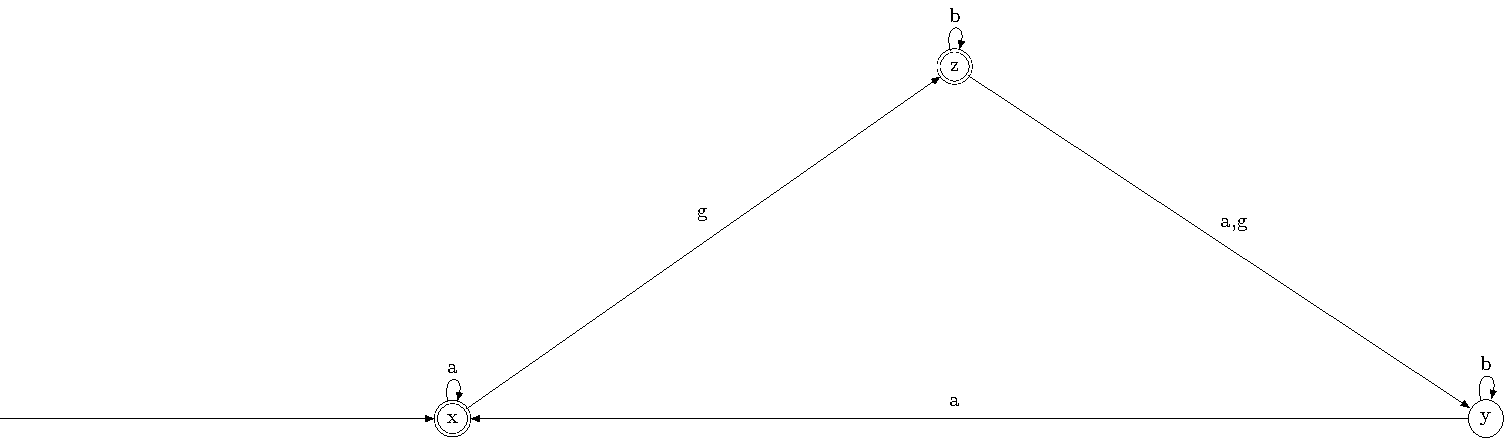
\includegraphics[width=0.5\textwidth]{automata/example/example.tikz}
  % \includetikzfigure[width=0.5\textwidth]{automata/example/example}
  \caption{Diagram representing the automaton from example \ref{ex:simpleAutomaton}}
  \label{fig:diagramExapleAutomata}
\end{figure}
We can also mark states that have some special meaning, a final state for instance. In this work, as in \cite{cassandras2009introduction} they are
  going to be identified by double circles.

  
  Now a deterministic Automaton can be defined:
\begin{definition}[Deterministic Automaton]
  \label{def:DeterministicAutomaton}~\\
  A Deterministic Automaton, denoted by G, is a five-tuple
  \[ G = (X,\Sigma,f, x_0,X_m)\] where:

  \indent X is the set of \textbf{states} \\
  \indent $\Sigma$ is the finite set of \textbf{events} associated with G\\
  \indent $f: X \times \Sigma \rightarrow X$ is the \textbf{transition function}  \\
  \indent $x_0$ is the \textbf{initial state} \\
  \indent $X_m \subseteq X $ is the set of \textbf{marked states}

\end{definition}


Other kinds of automata and operations between automata exist but are not going
to be used in this work, again \cite{cassandras2009introduction} present them.

\subsection{Petri Nets}
\label{sec:petriNets}
Another kind of representation of languages are Petri Nets, whose concept was created by C.A.Petri
in the early 1960's. Differently from the automata representation that are
basically formed from states, Petri nets are bipartite graphs, formed by nodes
called \emph{places} and \emph{transitions}.
Transitions represent the events that drive the system, and places represent the
conditions for these events to happen. The mechanism to represent the fulfilment
of the conditions
is named marking. A petri net is built over three basic concepts, the petri net
graph\slash structure, its marking and firing transitions.
The next subsections will be based on \cite{david2005discrete} and \cite{cassandras2009introduction}.

\subsubsection{Petri Net Graph}
\label{sec:petrinetGraph}
Similarly, arcs are used to connect
the nodes and have arrowheads to identify the direction,
but differently, all arcs must have exclusively one node at each end, that means
no arc is used to identify the initial state of a petri net. As said, a petri net is
bipartite graph, that means places can only connect to transitions and vice
versa. In this work as in \cite{david2005discrete} places will be represented by
circles and transitions by bars. 
\begin{figure}[H]
  \centering
  \begin{subfigure}[t]{0.45\textwidth}
  \centering
  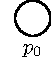
\includegraphics{petriNet/net/place.tikz}
  % \includetikzfigure[width=0.5\textwidth]{automata/example/example}
  \caption{A place.}
\end{subfigure}
~
\begin{subfigure}[t]{0.5\textwidth}
  \centering
  
\includegraphics{petriNet/net/transition.tikz}
  % \includetikzfigure[width=0.5\textwidth]{automata/example/example}
  \caption{A transition}
\end{subfigure}
  \caption{Component nodes of a petri net.}  
\end{figure}

The same way a function was created to define the transitions of states in an
automaton, two functions will be created to define the connections between places
and transitions. First we need to define the sets of places and transitions. $P$
is the set of places and $T$ the set of transitions. With this two sets we can
then define those functions. The first one represents the arcs
from places to transitions, and is denoted as $Pre: P \times T \rightarrow
\{0, 1\}$, the second one the arcs that connects transitions to places, denoted
as $Post: P \times T \rightarrow \{0,1\}$. The value $1$ is attributed to arcs
that exist and $0$ to the nonexistent ones.


\begin{example}[Simple Petri Net structure] ~\\
  \label{ex:simplePetriNetStructure}
  Given $P = \{p_0,p_1\}$, $T = \{t_0,t_1,t_2\}$ and the following transition
  functions:
  \begin{align*}
   Pre(p_0,t_0)& = 0  &  Post(p_0,t_1) &= 0 & Pre(p_1,t_0) &= 0 &  Post(p_1,t_1) &= 1 \\
   Post(p_0,t_0) &= 0  &    Pre(p_0,t_2) &= 0   & Post(p_1,t_0) &= 0   & Pre(p_1,t_2) &= 0\\
   Pre(p_0,t_1) &= 0    &  Post(p_0,t_2) &= 0  &  Pre(p_1,t_1) &= 0     &Post(p_1,t_2) &= 0\\
  \end{align*}
  We can represent this petri net structure with the diagram on \autoref{fig:simplePetriNetStructure}
\end{example}
\begin{figure}[H]
  \centering
  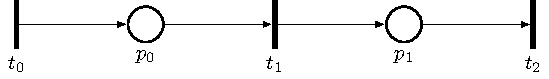
\includegraphics[width=0.5\textwidth]{petriNet/prepost/prepost.tikz}
  % \includetikzfigure[width=0.5\textwidth]{automata/example/example}
  \caption{Diagram representing the petri net structure from example \ref{ex:simplePetriNetStructure}}
\label{fig:simplePetriNetStructure}
\end{figure}
A drawback from the definition of this functions, is that is not possible to
have more than an arc linking two nodes, so we can generalize them to any natural number:
\begin{align*}
  Pre:  P \times T \rightarrow \mathbb{N}_0\\
  Post: P \times T \rightarrow \mathbb{N}_0
\end{align*}
with this new definition we can change the definition of $Post(p_1,t_1)$ from
$0$ to $2$ resulting on the following petri net structure.
\begin{figure}[H]
  \centering
  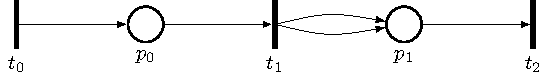
\includegraphics[width=0.5\textwidth]{petriNet/prepost/prepost2.tikz}
  % \includetikzfigure[width=0.5\textwidth]{automata/example/example}
  \caption{Diagram representing the petri net structure from example
    \ref{ex:simplePetriNetStructure}, but with $Post(p_1,t_1)=2$}
\label{fig:simplePetriNetStructureNatural}
\end{figure}
In order to reduce the number of arcs in a diagram, usually only one arc is
drawn and a label is added with the value of its respective function, if it is
greater than $1$, \autoref{fig:simplePetriNetStructureGeneralized} illustrates it:
\begin{figure}[H]
  \centering
  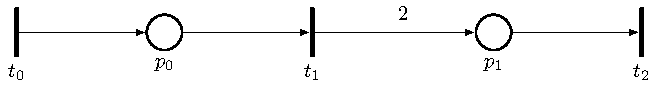
\includegraphics[width=0.5\textwidth]{petriNet/prepost/prepost3.tikz}
  % \includetikzfigure[width=0.5\textwidth]{automata/example/example}
  \caption{Same diagram as \autoref{fig:simplePetriNetStructureNatural} but with
    labeled arcs.}
\label{fig:simplePetriNetStructureGeneralized}
\end{figure}

\subsubsection{Marking}
\label{sec:marking}

As said in the beginning of this subsection marking is used as the mechanism to
represent if the condition of occurrence of a determined event is met or not.
But also it can be used to represent the state of the system. The mechanism
works as follows. Tokens can be designated to places and the way the tokens are
distributed among places is called the marking of a petri net graph. We can define a marking function $x :
P \rightarrow \mathbb{N}$ that denotes the number of tokens in a determined place.
In this
work, as in the majority of articles and books, the tokens will be
represented as black dots inside the places. 

The
\Autoref{fig:unmarked,fig:marked} show an unmarked and a marked petri net graph.
\begin{figure}[H]
\begin{subfigure}[t]{0.45\textwidth}
  \centering
  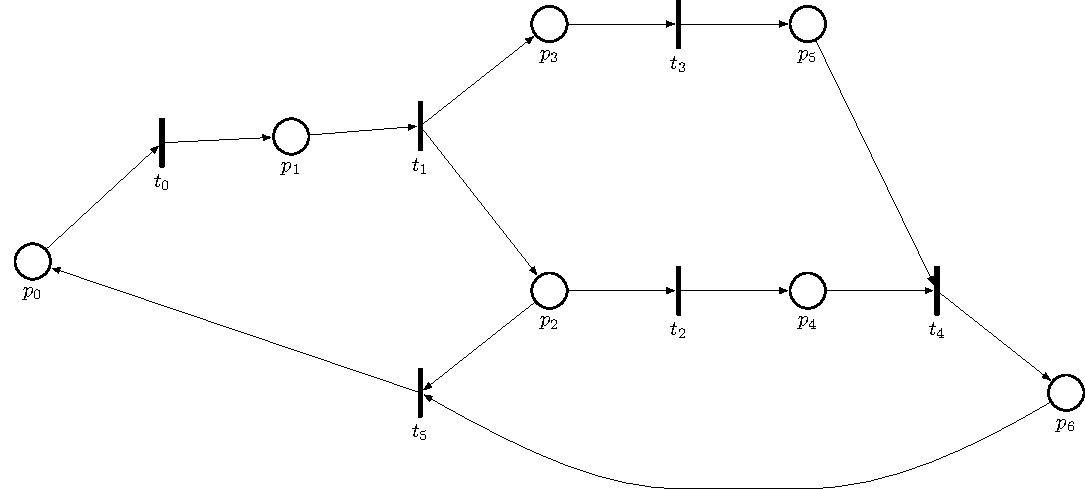
\includegraphics[width=\textwidth]{petriNet/net/unmarked.tikz}
  % \includetikzfigure[width=0.5\textwidth]{automata/example/example}
  \caption{Unmarked}
  \label{fig:unmarked}
\end{subfigure}
~
\begin{subfigure}[t]{0.45\textwidth}
  \centering
  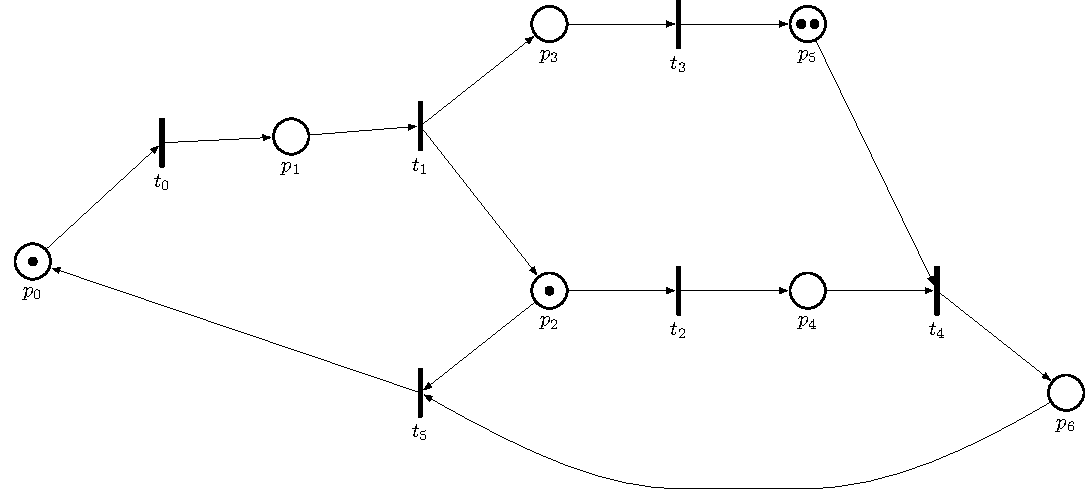
\includegraphics[width=\textwidth]{petriNet/net/marked.tikz}
  % \includetikzfigure[width=0.5\textwidth]{automata/example/example}
  \caption{Marked}
  \label{fig:marked}
\end{subfigure}
\caption{Example of unmarked and marked petri net graphs.}
\end{figure}

The marking of a petri net, can be represented as a
vector of the function $x$ applied on all places, for example the marking of the
\autoref{fig:marked} is the following vector $\mathbf{x}$

\begin{equation*}
\mathbf{x}=\begin{bmatrix}
  x(p_0)\\
  x(p_1)\\
  x(p_2)\\
  x(p_3)\\
  x(p_4)\\
  x(p_5)\\
  x(p_6)
\end{bmatrix} =
\begin{bmatrix}
  1\\
  0\\
  1\\
  0\\
  0\\
  2\\
  0
\end{bmatrix}
\end{equation*}

This vector $\mathbf{x}$, the marking of the petri net, can be identified as the
state of the petri net. So, different configurations of tokens mean different
states of the system, now we only need a way to change from a state to other, in
other words, move the tokens.

\subsubsection{Firing Transitions}
\label{sec:firingTransitions}
The mean of move the tokens is firing transitions. When an event  happens and
the corresponding transition is enabled, this transition is fired and tokens
are moved between places.
We can define the functions $I : T \rightarrow 2^P$ and $O : T \rightarrow 2^P$ that
describe the set of places considered as inputs and outputs of a transition: 
\begin{align*}
  I(t_j)= \{p \in P : Pre(p,t)> 0\}\\
  O(t_j)= \{p \in P : Post(p,t)> 0\}\\
\end{align*}
\begin{definition}[Enabled transition]
  \label{def:enabledTransition}~\\
  A transition is enabled if
  \[ x(p_i)\geq Pre(p_i,t_j) \text{ for all }{p_i \in I(t_j)}\]
  if $I(t_j)=\emptyset$, $t_j$ is always enabled. 
\end{definition}

And we can define the dynamic of the petri net, how the tokens move: 

\begin{definition}[Petri net dynamics]
  \label{def:petriNetDynamics}~\\
   It is possible to define a \emph{state transition}
  function, $f : \mathbb{N}^n \times T \rightarrow \mathbb{N}^n$  , where $n$ is
  the length of the state vector $\mathbf{x}$. This function $f$ is defined for
  a transition $t_j \in T$ if and only if this transition is enabled. If
  $f(\mathbf{x},t_j)$ is defined, then we create a new state vector
  $\mathbf{x}^\prime$:

  \[ x^\prime(p_i) = x(p_i) - Pre(p_i,t_j) + Post(p_i,t_j), i=1,\dots n \]
\end{definition}
  
As an example we can take \Autoref{fig:petriNetDynamics}:
\begin{figure}[H]
  \centering
 \begin{subfigure}[t]{0.45\textwidth}
  \centering
  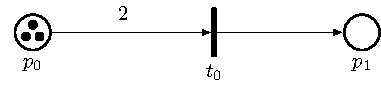
\includegraphics{petriNet/net/beforeFiring.tikz}
  % \includetikzfigure[width=0.5\textwidth]{automata/example/example}
  \caption{Before firing.}
  \label{fig:beforeFiring}
\end{subfigure}
~
\begin{subfigure}[t]{0.45\textwidth}
  \centering
  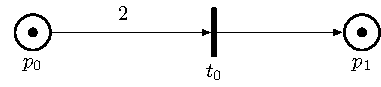
\includegraphics{petriNet/net/afterFiring.tikz}
  % \includetikzfigure[width=0.5\textwidth]{automata/example/example}
  \caption{After firing.}
  \label{fig:afterFiring}
\end{subfigure}
  \caption{Example of petri net Dynamic.}
  \label{fig:petriNetDynamics}
\end{figure}
The state before firing transition $t_0$ is $\mathbf{x}=\begin{bmatrix}3&
  0\end{bmatrix}^T$ and as we see $Pre(p_0,t_0)=2$ and $Post(p_1,t_0)=1$ so
applying the petri net dynamic we can find the next state $\mathbf{x}^\prime=\begin{bmatrix}1&
  1\end{bmatrix}^T$

Once all these fundamentals are presented we can finally define a Petri Net

\begin{definition}[Petri net]
  \label{def:petriNet}~\\
  A Petri net is defined as a five-tuple
  \[PN = (P,T,Pre,Post,\mathbf{x}_0)\]
  where: \\
  \indent $P$ is the set of \textbf{places} \\
  \indent $T$ is the set of \textbf{transitions} \\
  \indent $Pre$ is the \textbf{input incidence} function  \\
  \indent $Post$ is the \textbf{output incidence} function\\
\indent $\mathbf{x}_0$ is the initial marking of the net \\
And its dynamic is ruled by the \emph{state transition} function $f$ defined at \ref{fig:petriNetDynamics}.

\end{definition}

To make the connection between the Petri net and the events of the system, called $\Sigma$, the alphabet, we can
define a labeling function, $l : T^* \rightarrow \Sigma^*$ that makes the link between a
sequence of firing transitions and a sequence of events. But each transition
can only have one respective event. 

\begin{definition}[Labeled Petri net]
  \label{def:petriNet}~\\
  A Labeled Petri net is defined as a seven-tuple
  \[PN = (P,T,Pre,Post,\mathbf{x}_0,\Sigma,l)\]
  where: \\
  \indent $(P,T,Pre,Post,\mathbf{x}_0)$ is a Petri Net\\
  \indent $\Sigma$ is the set of \textbf{events} \\
  \indent $l$ is the \textbf{labeling} function  \\
\end{definition}

Usually the events are represented in the petri net graph over its respective
transition as shown in the \autoref{fig:labeledPetriNet}. This system has an alphabet
$\Sigma=\{a,b\}$ and labeling functions $l(t_0)=a$ and $l(t_1)=b$.

\begin{figure}[H]
  \centering
  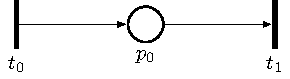
\includegraphics{petriNet/labeled/labeled.tikz}
  % \includetikzfigure[width=0.5\textwidth]{automata/example/example}
  \caption{Labeled Petri net.}
  \label{fig:labeledPetriNet}
\end{figure}

\section{Control Interpreted Petri Nets}
\label{sec:cipn}
One of the greatest uses of Petri Nets, besides modeling a system, is its
ability to model the control of a system. For this intent we use Control Interpreted Petri nets. It is an
extension from the labeled Petri net, we add actions for places, so it is
possible to change the outputs of the system, conditions to the transitions, so it
is possible to change the state of the control based on the inputs of the
system, and even the ability to delay the firing transitions based on time.
Another artifice used is an inhibitor arc, that prevents the firing of a
transition based on the marking of the corresponding place.

\begin{definition}[Control Interpreted Petri net]
  \label{def:cipn}~\\
  A Labeled Petri net is defined as a seven-tuple
  \[PN = (P,T,Pre,Post,\mathbf{x}_0,In,\Sigma,C,l_C,D,L_D,A,I_A)\]
  where: \\
  \indent $(P,T,Pre,Post,\mathbf{x}_0)$ is a Petri Net\\
  \indent $In$ is the \textbf{inhibitor arc} function that prevents the
  enablement of transitions \\
  \indent $\Sigma$ is the set of \textbf{events} associated to transitions \\
  \indent $C$ is the set of \textbf{conditions} associated to transitions \\
  \indent $l_C$ is the \textbf{labeling} function that associates a transition
  with events and conditions from $\Sigma$ and $C$\\
  \indent $D$ is the set of \textbf{delays} associated to transitions \\
  \indent $l_D$ is the \textbf{labeling} function that associates a transition with a delay from $D$ \\
  \indent $A$ is the set of \textbf{actions} associated to places \\
  \indent $l_A$ is the \textbf{labeling} function that assigns actions from $A$ to a place \\
\end{definition}
The definition of $In : (P \times T )\rightarrow\mathbb{N}$ is that a transition
$t_j$ is inhibited if $x(p_i)\geq In(p_i,t_j)$. Inhibitor arcs are not used in
this work but usually they are represented with an arc with a circle in one of
its ends, as shown in \autoref{fig:inhibitor}.

\begin{figure}[H]
  \centering
  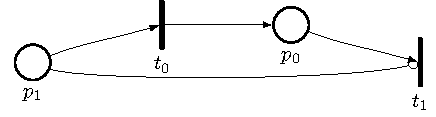
\includegraphics{petriNet/inhibitor/inhibitor.tikz}
  % \includetikzfigure[width=0.5\textwidth]{automata/example/example}
  \caption{Example of Petri net with inhibitor arc.}
  \label{fig:inhibitor}
\end{figure}
As we can see from the definition there are two labeling functions to connect 
transitions, $l_C$ and $l_D$. The $l_c$ is defined for transitions with no
firing delay and $l_D$ for transitions with firing delay.

The labeling function $l_C : T^0\rightarrow(\Sigma \times C)$ defines a pair of
event and boolean condition from $\Sigma$ and $C$ respectively. A transition
$t_i$ belonging to $T^0$ (a subset of $T$ that represents the transitions with
no time delay) has a corresponding event, condition tuple $(\sigma_i,c_i)$
For example, take a transition $t_0$, $\Sigma =\{\sigma_0\}$ and $C=\{c_0\}$. If
a function $l_c(t_0)=(\sigma_0,c_0)$ is defined, this transition will be fired
when the condition $c_0$ is true and the event $\sigma_0$
happens, but obviously, if and only if this transitions is enabled and not
inhibited. The transition $t_0$ is represented graphically as shown in \autoref{fig:condition}

\begin{figure}[H]
  \centering 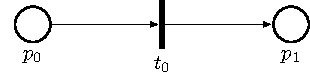
\includegraphics[width=0.3\textwidth]{petriNet/cipn/condition.tikz}
  \caption{Representation of new labeling function}
  \label{fig:condition}
\end{figure}

If the event is missing from the representation of the transition, it is equal
to the $\lambda$
, the always occurring event. And if the condition is missing, that means it is
equal to $1$, it is always $true$. If both are missing, that means the
transition will be automatically executed if it is enabled. 

By the other hand, the labeling function $l_D : T^D \rightarrow D$, defines a delay for the
transition to be fired. A timed transition $t_i$, a transition in $T^D$ (a subset of T
that represents the transitions with a time delay), has a corresponding delay
$d_i$. As an example, take a timed transition $t_1$ and $D=\{d_1\}$, after the
enablement of the transition, it takes $d_1$ time units in order to be fired. In
this work timed transitions are represented as bars slightly larger than normal
conditions. An example of this representation we can see \autoref{fig:timedtransition}

\begin{figure}[H]
  \centering 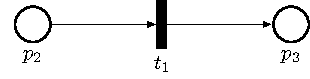
\includegraphics[width=0.3\textwidth]{petriNet/cipn/timedtransition.tikz}
  \caption{Representation of a timed transition.}
  \label{fig:timedtransition}
\end{figure}
Another labeling function that was created is $l_A : P\rightarrow 2^A$,
assigning a set of actions belonging to $A$ to a place. Actions can be impulse actions or continuous. A
continuous action happens always that the marking of a place is greater than 0,
$x(p_i)>0$, an impulse action, on the other hand, happens only when the marking of
the place changes from 0 to a value greater than 0. 
Actions are represented graphically as labels in places. Impulse actions are differed by a star (*) at its end. So an action $F$ is
continuous and $B^*$ is an impulse action. 
\autoref{fig:actions} show a representation of a Place with both kinds of actions.
\begin{figure}[H]
  \centering 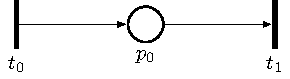
\includegraphics[width=0.3\textwidth]{petriNet/cipn/actions.tikz}
  \caption{Representation of labeling of Actions.}
  \label{fig:actions}
\end{figure}

Although these representations exist, in this work events, conditions and
actions labels are suppressed from the diagrams and tables accompany the drawings
showing the meaning of the transitions (firing events and conditions) and places
(Actions). This choice was made because when the controlled interpreted Petri nets
are very
large as the ones shown in the next chapters, if the events, conditions and
actions labels are long they can increase the size of the
diagram.

To illustrate this better we give an example based on one example from \cite{david1989grafcet}.
\begin{example}[Loading of a wagon] ~\\
  \label{ex:loadingOfAWagon}
We consider the system represented by the scheme in
\autoref{fig:cipnexamplescheme}. A wagon can be moved between the points $a$ and
$b$, using the inputs $L$ and $R$ (moving it to the left or right,
respectively). At point $a$ there is a button $m$ that can be pressed by an
operator and a limit switch called $a$ that is activated when the wagon is on
the left. At point $b$, an homonym limit switch is placed and activated when the
wagon is on the right. There is a hopper that can
be opened when the input $Open$ is turned on and closed when not.If it is opened
its content is poured. There is also a
button $p$ that is activated when the weight applied over the plate is equal or
greater to the weight of a full wagon. 

The objective of the control is, when the wagon is in its leftmost position and
the button $m$ is pressed, it moves to the right, stops at $b$, the hopper is
opened and the wagon is loaded, when it is completely full it moves to the left
and it stops at $a$ waiting to be unloaded and for a next press of $m$ to recommence
the loop. 
\end{example}


\begin{figure}[H]
  \centering \includegraphics[width=0.8\textwidth]{cipnExample/scheme.tikz}
  \caption[cipnexample]{Example of System to be controlled by the Petri Net}
  \label{fig:cipnexamplescheme}
\end{figure}
From the description of the control it is possible to create a Control Interpret
Petri Net to describe it, as the one in \autoref{fig:cipnexample}


\begin{figure}[H]
  \centering 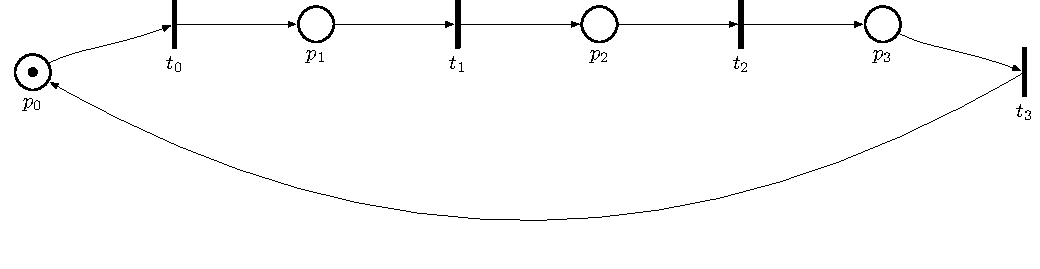
\includegraphics[width=0.8\textwidth]{cipnExample/cipn.tikz}
  \caption[cipnexample]{Example of Control Interpreted Petri Net to control
    system in \autoref{fig:cipnexamplescheme}}
  \label{fig:cipnexample}
\end{figure}

The meaning\slash description of each place and transition is given by the
following tables:

\begin{table}[htbp]
\caption{Control Interpreted Petri Net Example Places.}
\centering
\begin{tabular}{M{5cm}M{10cm}}
Places & Meaning\\
\hline
\hyperlink{cipnExampleNet:p0m1}{\hypertarget{cipnExampleTable:p0m1}{$p_{0}$}} & System Stopped\\
\hyperlink{cipnExampleNet:p1}{\hypertarget{cipnExampleTable:p1}{$p_{1}$}} & R (Car Moving to the Right)\\
\hyperlink{cipnExampleNet:p2}{\hypertarget{cipnExampleTable:p2}{$p_{2}$}} & Open (Container Opened)\\
\hyperlink{cipnExampleNet:p3}{\hypertarget{cipnExampleTable:p3}{$p_{3}$}} & L (Car Moving to the Left)\\
\end{tabular}
\end{table}

\begin{table}[H]
\caption{Control Interpreted Petri Net Example Transitions.}
\centering
\begin{tabular}{M{5cm}M{10cm}}
Transitions & Meaning\\
\hline
\hyperlink{cipnExampleNet:t0}{\hypertarget{cipnExampleTable:t0}{$t_{0}$}} & m (filling request)\\
\hyperlink{cipnExampleNet:t1}{\hypertarget{cipnExampleTable:t1}{$t_{1}$}} & b (Right Limit Switch)\\
\hyperlink{cipnExampleNet:t2}{\hypertarget{cipnExampleTable:t2}{$t_{2}$}} & p (Car is Full)\\
\hyperlink{cipnExampleNet:t3}{\hypertarget{cipnExampleTable:t3}{$t_{3}$}} & a (Left Limit Switch)\\
\end{tabular}
\end{table}


In this work as in the usual boolean notation, when just the name of a variable is given in a table it means the
variable is equal to true, and when there is a bar in its top it is equal to
false, so they determine conditions. E.g.: $b$ and $\overline{b}$.
And when a variable is preceded by $\uparrow$ and $\downarrow$, they  determine
events corresponding to its raising and falling edge.

\usetikzlibrary{arrows,shapes,circuits.plc.ladder,external}

\section{Implementation of Control Interpreted Petri Nets}
\label{sec:implementPetriNets}
Once the control of a system is modeled by a \CIPN, it
is needed to implement the control in a real controller. The most used
controllers in the industry are \PLCs. The international standard IEC 61131,
defines all the standards for \PLCs, and its third part (IEC 61131-3) defines
five languages to program \PLCs: \LD, Function Block Diagram
(FBD),  Structured Text (ST), Instruction List (IL) and Sequential Function
Chart (SFC). One of the most used in the industry is \LD, because of its
resemblance with electric connections. So we are going to use \LD{} to implement the
control designed with the \CIPN.

\subsection{Ladder Logic}
\label{sec:ladder}

The ladder logic is based on two components, contacts and coils. Their terminals are
interconnected to transmit boolean signals. This connection is similar to the
ladder physical implementation, from where came its inspiration, the components
were connect to boards and they formed electric circuits, turning on and off
motors and other actuators, based on the combination of its inputs. The name
Ladder comes from the resemblance between its structure (circuits formed in
parallel one above the other) and a ladder, so each circuit is called a Rung by analogy. The logic
values in a \LD{} rung
are transmitted from the left to the right of the diagram. The components let
the logic ``current'' flow from its left terminal to the right terminal
depending on some conditions, and these conditions vary from component to
component.
The rungs are executed one by one and once the very last rung is executed,
the first rung is re-executed, thus creating an infinite loop. 
 The graphical representation of the most used types of contacts and coils
can be seen in \Autoref{fig:contacts,fig:coils}

\newlength{\ladderskip}
\newlength{\ladderrungsep}

% Types of Contacts
\begin{figure}[H]
\begin{subfigure}[t]{0.45\textwidth}
  \centering \includegraphics{ladder/contactNO.tikz}
  \caption{Normally Opened Contact.}
  \label{fig:contactNO}
\end{subfigure}
~
\begin{subfigure}[t]{0.45\textwidth}
  \centering \includegraphics{ladder/contactNC.tikz}
  \caption{Normally Closed Contact.}
  \label{fig:contactNC}
\end{subfigure}
\vspace{1em}

\begin{subfigure}[t]{0.45\textwidth}
  \centering \includegraphics{ladder/contactP.tikz}
  \caption{Positive Edge Contact.}
  \label{fig:contactP}
\end{subfigure}
~
\begin{subfigure}[t]{0.45\textwidth}
  \centering \includegraphics{ladder/contactN.tikz}
  \caption{Negative Edge Contact.}
  \label{fig:contactN}
\end{subfigure}

  \caption{Types of Contacts.}
  \label{fig:contacts}
\end{figure}

% Types of Coils
\begin{figure}[H]
\begin{subfigure}[t]{0.45\textwidth}
  \centering \includegraphics{ladder/coilNO.tikz}
  \caption{Coil.}
  \label{fig:contactNO}
\end{subfigure}
~
\begin{subfigure}[t]{0.45\textwidth}
  \centering \includegraphics{ladder/coilNC.tikz}
  \caption{Negated Coil.}
  \label{fig:contactNC}
\end{subfigure}
\vspace{1em}

\begin{subfigure}[t]{0.45\textwidth}
  \centering \includegraphics{ladder/coilSet.tikz}
  \caption{Set (latch) Coil.}
  \label{fig:contactP}
\end{subfigure}
~
\begin{subfigure}[t]{0.45\textwidth}
  \centering \includegraphics{ladder/coilReset.tikz}
  \caption{Reset (unlatch) Coil.}
  \label{fig:contactN}
\end{subfigure}

  \caption{Types of Coils.}
  \label{fig:coils}
\end{figure}

\subsubsection{Contacts}
Contacts represent the conditions of the ladder logic depending on inputs. These inputs can be any variable in a
\PLC, an external input ( sensors of the system to be controlled), a variable stored in memory or the current
value sent to an output from the \PLC. A normally opened contact
activates its right terminal (set it to $true$) if the logic value in its left terminal
is $true$ and its corresponding input is equal to $true$ 
A normally closed contact activates its right terminal if the logic value in its
left terminal is $true$ and its corresponding input is equal to $false$.
The Positive Edge contact activates its right terminal only in the instant that
its input change from logic value $false$ to $true$, if the logic value in its
left terminal is $true$. And the Negative Edge contact activates its right
terminal only in the instant that its input change from logic value $true$ to
$false$.

As we can see, positive and negative contacts can be used to represent raising ($\uparrow$)
and falling edge  ($\downarrow$) events and normally opened and closed contacts
to represent conditions (and their negation).

\subsubsection{Coils}

Coils, by the other side represent the actuation in outputs. These
outputs can be a variable stored in memory or the outputs
of the controller (actuators of the system to be controlled, for instance). 
A coil sets its output variable to true if the logic value of its left terminal is $true$,
and sets the output to $false$ otherwise.
A negated coil does the exact opposite, sets the output value to true if the logic
value of its left terminal is $false$ and sets it to $true$ if the logic is
$true$.

A set coil (or latch) sets its output variable to $true$ if the logic value of its
terminal is $true$ and it remains $true$ until the variable is reset.
And a reset coil (or unlatch) sets its output variable to $false$ if the logic
value of its terminal is $true$ and it remains $false$ until the variable is
set.

\subsubsection{Combinational Logic}
In boolean logic, in order to show functional completeness, it is need to show a
complete set of connectives ( a set that can create all other logic connectives
as a combination of its elements ). A well-know complete set is $S=\{AND,NOT\}$,
binary conjunction and negation.
To show that the ladder logic is functional complete we need only to present how
to construct this two connectors in it.
The conjunction of two inputs, can be made using two contacts in series, as
shown in \autoref{fig:ladderSeries}
\begin{figure}[H]
  \centering \includegraphics{ladder/series.tikz}
  \caption{And logic in a Ladder rung.}
  \label{fig:ladderSeries}
\end{figure}
In this case C will only be activated if A and B are equal to $true$. ($C=AB$)

The negation of a variable can be achieved by the use of a normally closed
contact (\autoref{fig:ladderNot}).
\begin{figure}[H]
  \centering \includegraphics{ladder/not.tikz}
  \caption{Not logic in a Ladder rung.}
  \label{fig:ladderNot}
\end{figure}
C will only by activated if A is $false$. ($C=\overline{A}$)

Although all logic connectives can be constructed with this two connectors, the
OR connector can be achieved by the use contacts in parallel (\autoref{fig:ladderParallel}).
\begin{figure}[H]
  \centering \includegraphics{ladder/parallel.tikz}
  \caption{Or logic in a Ladder rung.}
  \label{fig:ladderParallel}
\end{figure}



\subsubsection{Function Blocks and extensions}
In order to increase functionality some function blocks and 
extensions to contacts were created. We can see examples of theses blocks and
contacts in the next figure:

\begin{figure}[H]
   \centering
\begin{subfigure}[t]{0.45\textwidth}
  \centering \includegraphics{ladder/ctu.tikz}
  \caption{Up counter.}
  \label{fig:ctu}
\end{subfigure}
~
\begin{subfigure}[t]{0.45\textwidth}
  \centering \includegraphics{ladder/ton.tikz}
  \caption{On-delay timer.}
  \label{fig:ton}
\end{subfigure}

\begin{subfigure}[t]{0.45\textwidth}
  \centering \includegraphics{ladder/comp.tikz}
  \caption{Less or equal comparator.}
  \label{fig:comp}
\end{subfigure}
  \caption{Examples of function blocks.}
  \label{fig:functionBlocks}
\end{figure}

Up counters (\autoref{fig:ctu}) save the value of a counter in a $CV$ variable. Every raising edge
on input $CU$ it increments $CV$ value. If $CV=PV$, the logic value of output $Q$ 
is set to $0$. When the input $R$ is true $CV$ value is set to $0$ and the
output $Q$ set to false.

On-delay timers (\autoref{fig:ctu}) set a timer when input $IN$ is $true$
and save it to $ET$. If $ET=PT$, the logic value of output $Q$ is set to $true$.
But if, meanwhile the counting, the value of $IN$ returns to $false$, $ET$ is reset to
$0$.

Comparator contacts as the less or equal comparator in \autoref{fig:comp}, work
similarly to contacts, but instead of an input as a condition, there are two
inputs ($value1$ and $value2$) and the condition is a comparison between both of
them. In this case, the contact is activated once its left terminals' logic
value is $true$ and $value1\leq value2$.

Other blocks and functions can be found in the IEC 61131-3, as adders,
subtractors, communication blocks etc.

\subsection{Conversion from \CIPN{} to \LD}
\label{sec:cipnToLD}

A simple method of conversion from \CIPN{} to \LD{} is presented in
\cite{moreira2013bridging}.

It consists in dividing the \CIPN{} in 4 modules:
\begin{enumerate}
\item A module of external events\\
  To create conditions to the firing of transitions based on external events
  (inputs)
\item A module of firing conditions\\
  To indicate what condition will be fired using the $Pre$, and $In$ functions, the conditions found on the
  last module and time delays (if it is a timed transition 
  )
\item A module of Petri Net dynamics\\
Uses the $Pre$ and $Post$ functions to determine the tokens ``motion''
\item A module of actions\\
  Determines the places where each action is performed.
\end{enumerate}
In this work, the external events and firing conditions was combined in order to
reduce the size of the program. But every module will be described as in
\cite{moreira2013bridging}.

\subsubsection{External events}
As external events are associated with positive and negative edge of the inputs
of the system, in this module, positive and negative edge contacts are used to
detect the rising and falling edge events, and they are stored in variables
using coils, a variable is created for every event.
For visibility's and organisation's sake a rung is used for each event,
resulting $|\Sigma|$ rungs. 
\subsubsection{Firing Conditions}
As said in \ref{sec:cipn}, for a transition $t_j$ to be fired, first it needs to be
enabled ($x(p_i)\geq Pre(p_i,t_j)$ for all $p_i\in I(t_j)$), not inhibited
($x(p_i)< In(p_i,t_j)$ for all $p_i\in I(t_j)$) and the conditions and events
$\sigma_jc_j$ are met or the delay $d_j$ is elapsed, depending on the kind of
transition.
As places can have multiple tokens, we can use $int$ variables to store the
number of tokens, and comparator contacts to determine if the transitions are
enabled and not inhibited.
When a place can only bear at most one single token for all markings of the
Petri net, a $bool$ variable can be used to store the number of tokens, in this
case a single normally open contact can be used to determine if there is a token
in that place.
The time delays are implemented using on-delay
timers. The state of fulfilment of the conditions is stored in variables, one
for each transition.
Similarly, for organisation's sake a rung is used for each transition, resulting
$|T|$ rungs.
\subsubsection{Petri Net Dynamics}
In this module the dynamic of the tokens is implemented. If the condition for
the firing of a transition is fulfilled (represented by normally open contacts), adders and subtractors
can be used to represent the movement of tokens, increasing and decreasing the
values from the $int$ variables that represent the marking
of each place, if their capacity is greater than one, if not they are
represented by boolean variables, and instead Set and Reset coils can be used to
represent a token entering a place and a token exiting another, respectively.
Again, for organisation's sake a rung is associated for each transition,
resulting $|T|$ rungs.

\subsubsection{Actions}
In the Action module, we use coils to act on the outputs. Depending on the type
of action and the logic of the control, set\slash reset coils or normal coils
can be used. The condition to activate\slash deactivate the output is the
presence of a token in the places where the action is performed, this can be
achieved by comparing the numbers of tokens in a place. If the tokens of a
place is represented by an $int$ variable, we use greater or equal comparators,
but if it is represented by a $bool$ variable, a normally opened contact is
enough. If the action is an impulse action we can put a positive edge in series
with the places contact or the comparator.

Differently from the original article, we will use one rung per
each action in A, resulting in $|A|$ rungs. This is made because in
\cite{renault2017regles} it is recommended to perform an action in only one
rung, and group the conditions using OR connectors.
In the industry this is important in order to reduce errors and to ease the
debugging process.

\subsubsection{Example}

An example of this conversion can be given using the same \CIPN{} from example 
\ref{ex:loadingOfAWagon}. As said, the external events and firing condition
modules are grouped in same module in this work. The converted Ladder Logic
can be seen in \autoref{fig:cipnexampleLadder}.
\begin{figure}[H]
  \centering \includegraphics{cipnExample/cipnLadder.tikz}
  \caption[cipnexample]{Example of Control Interpreted Petri Net converted to
    Ladder.}
  \label{fig:cipnexampleLadder}
\end{figure}

\subsection{Petri Net divided in multiple PLCs}
\label{sec:multiplePlcs}
A problem that can occur, is the case where a \CIPN{} must be divided in
multiple \PLCs, because of how the assembling of the plant was (some
inputs\slash outputs are only
connected to a single \PLC, and other inputs\slash outputs to another \PLC),
this division can be arbitrarily decided by the
person who will implement the control.

In \autoref{fig:communicationPlcPN}, it is shown an example of a \CIPN{} divided
between 2 \PLCs.
As we can see, in \Autoref{fig:communicationPlcPN1,fig:communicationPlcPN2}
there are dotted transitions and places. In this work, we will represent as
dotted, transitions and places that are part of another section of the Petri
Net. They are not represented in the same figure, 
but the arcs show the connection between the sections of the net, showing that
when connected they form a complete Petri net. In the digital form\footnote{Available at: \url{https://github.com/Accacio/docsTCC/raw/master/monografia.pdf}}  of this thesis it is possible to travel between
figures that are not in the same page just by clicking in the name of the
corresponding dotted place\slash transition.
\begin{figure}[H]
  \centering
  \begin{subfigure}[t]{0.5\textwidth}
    \center
    \includetikzfigure[width=\textwidth]{communicationPlcPN/communicationPlcPN}
    \caption{Petri Net on PLC 1.}
    \label{fig:communicationPlcPN1}
  \end{subfigure}%
  ~
  \begin{subfigure}[t]{0.5\textwidth}
    \centering
    \includetikzfigure[width=\textwidth]{communicationPlcPN/communicationPlcPN1}
    \caption{Petri Net on PLC 2.}
    \label{fig:communicationPlcPN2}
  \end{subfigure}
  \caption{Example of Petri Net divided between 2 PLCs.}
  \label{fig:communicationPlcPN}
\end{figure}

In order to solve the problem of communication caused by the division, there are
different ways, one of them is the method shown by \cite{antunesfloriano2019sincronizacao}, where
different sections are synchronised in a distributed manner using common places.
In this work, a master\slash slave approach was used. CLP1 was considered as the
master and CLP2 as a slave. For the master, it is created another module
called ``Data Sending\slash Receiving'', divided in 2 parts, the first that
happens before all other modules, with the objective of getting all needed
variables from other \PLCs, and another part, that happens after all other
modules, with the objective of sending variables to all other \PLCs.
By the other side, the slaves have 2 modules, one at the beginning, called
``Prepare Received Data'' and another at the very end called ``Prepare Data to
Send'', in which the data received from the master is prepared to be used and
the data is prepared to be sent to master.

The communication between \PLCs{} can be made using Profinet protocol, and if we
take for instance Siemens \PLCs, they have two function blocks called ``Get'' and
``Put'', that are used to establish data transfer between two \PLCs{} using the
Profinet protocol. Tutorials on how to configure this blocks can be found on \citep{antunesfloriano2019sincronizacao,oliveira2016protocolo,rochapereira2019automacao}.


The basic idea is to transfer the state of the variables that determine the
conditions of firing transitions between both \PLCs. The problem is that as the
two \PLCs are not in sync, the condition of a firing transition could change in
the middle of the logic. So, in order to circumvent it, we can duplicate those
variables in the slave PLC, and in the ``Prepare Received data'' module update
the values of these variables (using positive edges contacts), forcing them to
be updated only once in each loop and when their value are changed from $0$ to
$1$.

When a transition change the value of tokens in more than one \PLCs, as $t_1$,
an auxiliary variable is created in order to create a kind of
acknowledgement\slash permission 
from the master, as an ``ok, you can proceed'' to the slaves to perform the
dynamic of that transition.

The example of those three new modules are shown in \autoref{fig:communicationPlcPNLadder}

\begin{figure}[H]
  \centering
  \begin{subfigure}[t]{0.45\textwidth}
    \centering
    \includegraphics{communicationPlcPN/communicationPlcPNLadder.tikz}
    \caption{Ladder Logic on PLC 1.}
    \label{fig:communicationPlcPN1Ladder}
  \end{subfigure}%
  \hfill
  \begin{subfigure}[t]{0.45\textwidth}
    \centering
    \includegraphics{communicationPlcPN/communicationPlcPN1Ladder.tikz}
    \caption{Ladder Logic on PLC 2.}
    \label{fig:communicationPlcPN2Ladder}
  \end{subfigure}
  \caption{Example of Petri Net divided between 2 PLCs.}
  \label{fig:communicationPlcPNLadder}
\end{figure}
  
As we can expect, this kind of logic of master\slash slave works well when
there are 2 \PLCs, but when there are more \PLCs, this centralised approach
creates a single point of failure and as the master \PLC{} works as a hub, it
increases the communication delay. When there are more than two \PLCs{} it is
preferable to use a distributed approach as the one shown in
\cite{antunesfloriano2019sincronizacao}.

\section{Identification}
\label{sec:identification}

Once the control is implemented and the system is working as it should, we
arrive at the objective of this work, the identification of the system.
As said in the introduction, this work is based on \cite{moreira2018enhanced}.
In this article, a new model for \DES{} identification is proposed, called
\glsreset{DAOCT}\DAOCT. This model was created with aim of fault detection based
on the observation of the fault free behaviour of the system, as in the models
proposed by 
\cite{roth2009fdi} and \cite{klein2005fault}, but its use of paths increases the
efficiency for fault detection when compared with the latter articles.

This fault free observation is made by the acquisition of the observable signals
of the system (controller inputs and outputs) for a sufficiently long
period of time while the system works normally. These signals can be seen on \autoref{fig:obsSignals}.

\begin{figure}[H]
  \centering
  \begin{tikzpicture}
        % \draw[help lines,xstep=1,ystep=1] (0,0) grid (10,10);
        % \foreach \x in {0,1,...,10} { \node [anchor=north] at (\x,0) {\x}; }
        % \foreach \y in {0,1,...,10} { \node [anchor=east] at (0,\y) {\y}; }
        
        \draw[ultra thick,rounded corners] (3.5,0) rectangle (6.5,1.5);
        \draw[ultra thick,rounded corners] (0.5,2) rectangle (3.5,3.5);
        \draw[ultra thick,rounded corners] (6.5,2) rectangle (9.5,3.5);
        \draw[ultra thick,rounded corners] (3.5,4.5) rectangle (6.5,6);
        \draw (5,5.25) node {Controller};
        \draw (5,0.75) node {Plant};
        \draw (2,2.75) node {Actuators};
        \draw (8,2.75) node {Sensors};

        % actuators to plant
        \draw[->,>=stealth, very thick] (2,2) -- (2,0.75) -- (3.5,0.75);

        % controller to actuators
        \draw[->,>=stealth, very thick] (3.5,5.25) -- (2,5.25) -- (2,3.5);

        % Plant to sensors
        \draw[->,>=stealth, very thick] (6.5,0.75) -- (8,0.75) -- (8,2);

        % Sensors to controller
        \draw[->,>=stealth, very thick] (8,3.5) -- (8,5.25) -- (6.5,5.25);

        \draw[->,>=stealth, very thick] (2,4) -- (10,4);
        \draw[fill] (2,4) circle(.05);

        \draw[->,>=stealth, very thick] (8,4.5) -- (10,4.5);
        \draw[fill] (8,4.5) circle(.05);

        \draw (11,4.5) node {Observed};
        \draw (11,4.15) node {signals};

        \draw (1.5,5.75) node {Controller outputs};
        \draw (8.5,5.75) node {Controller inputs};

    \end{tikzpicture}
  \caption{Observed Signals in a closed-Loop \DES.}
    \label{fig:obsSignals}
  \end{figure}

First, we assume the controller have $m_i$ binary inputs, $i_h$, for $h=1,\dots,m_i$ and $m_o$ binary
outputs, $o_h$, for $h=1,\dots,m_o$, and we create a Input\slash Output vector called $\mathbf{u}$, that varies with
time:

\begin{equation*}
\mathbf{u}(t_1)=
\begin{bmatrix}
  i_1(t_1)&
  \dots&
  i_{m_i}(t_1)&
  o_1(t_1)&
  \dots&
  o_{m_o}(t_1)
\end{bmatrix}^T
\end{equation*}
\newcommand{\vu}{\mathbf{u}}
 This vector $\mathbf{u}(t)$ represents the status of the system in a instant
 $t$. In the \DAOCT model, only untimed system models are considered, thus
 the status of the system can only be modified via system events, $\sigma$. To
 reduce the size of the notation $\mathbf{u}(t)$ is going to be represented as $\vu_t$. The
 transition between status in $t_i$ and $t_j$ is represented as ($\vu_i,\sigma,\vu_j$). If we have a sequence of
 $l$ input\slash output vectors, we have an observed path of the system,
 $p=(\vu_1,\sigma_1,\vu_2,\sigma_2,\dots,\sigma_{l-1},\vu_l)$.
So, if we observe multiple paths meanwhile our observation process, we can
create multiple paths
$p_i=(\vu_{i,1},\sigma_{i,1},\vu_{i,2},\sigma_{i,2},\dots,\sigma_{i,l_i-1},\vu_{i,l_i})$,
for $i=1,\dots,r$, where $r$ is the number of observed paths, and $l_i$ is the
number of vertices in each path $p_i$.

Supposing that all paths begin with the same I\slash O vector, that means, all
observations begin from the same status, it is possible to associate to each
path $p_i$ a sequence of events and a sequence of I\slash O vectors, called,
$s_i$ and $\omega_i$, and they are defined as:
\begin{align*}
  s_i&= \sigma_{i,1}\sigma_{i,2}\dots\sigma_{i,l_i-1} \\
  \omega_i&= \vu_{i,1}\vu_{i,2}\dots\vu_{i,l_i}
\end{align*}
Using these observed sequences of events $s_i$, we can define a language
, called observed language, $L_{Obs}$:

\begin{equation}
  L_{Obs}:= \bigcup^r_{i=1}\overline{\{s_i\}}
\end{equation}
\begin{observation}
If any sequence $s_i$ is the prefix of another sequence $s_j$, the path $p_i$ should
be discarded, along with $s_i$ and $\omega_i$, since it does not present any new
information for the identification process.
\end{observation}
The objective of identification is to find a model with a language that
can simulate this observed language. This language of the identified model is
called $L_{Iden}$.
We can describe this relation between these languages as $L_{Obs} \subseteq
L_{Iden}$.
As said in
\cite{moreira2018enhanced}, in finite time only part of the sequences  of events
the system can generate are observed. So we can define a language $L_{Orig}$,
the original language generated by the system, that we is never known.

From $L_{Orig}$ and $L_{Iden}$, we can define another language, an exceeding
language $L_{Exc}$, that is, part of the identified language that is not present in the
original language, $L_{Exc}=L_{Iden}\backslash L_{Orig}$.  The
relation between $l_{Orig}$ and $l_{Obs}$ is $L_{Obs} \subset L_{Orig}$. And from
these two languages we can define another language $L_{OrigNI}$, part of the
original language that was not identified, $L_{OrigNI}=L_{Orig}\backslash L_{Iden}$
The relation between all these languages is shown in \autoref{fig:languagesVenn}.

\usetikzlibrary{patterns}
\begin{figure}[H]
  \centering \includegraphics[width=0.5\textwidth]{vennDiagramLanguages.tikz}
  \caption{Venn diagram showing the relation between $L_{Orig}$, $L_{OrigNI}$,
    $L_{Obs}$, $L_{Exc}$ and $L_{Iden}$}
  \label{fig:languagesVenn}
\end{figure}
As $L_{Exc}$ represents a part of the identified language that is not part of
the original language, some faulty sequences will not be detected, as they are
part of the identified language. So in order to reduce the number of these non
detected faults, $L_{Exc}$ should have a cardinality as close to $0$ as it is
possible, this is possible by creating identification models that generate
smaller $L_{Exc}$.

And as $L_{OrigNI}$ represents the part of the original system that was not
identified, that means some sequences present on the fault-free behaviour of the
system will be detected as faults, generating false alarms. This language should
also be reduced, so the false alarms generated are reduced. As the original
language of the system is never known, it is very difficult to know for sure if
$L_{OrigNI}$ is small or not. \cite{klein2005fault} show that if a system is
observed for a sufficiently long time, there exists a number $n_0\in \mathbb{N}$
such that $L_{Orig}^{\leq n_0}\backslash L_{Obs}^{\leq n_0}\approx \emptyset$,
where $L_{Orig}^{\leq n_0}$ and $L_{Obs}^{\leq n_0}$ denote the languages formed
by all sequences of events of length smaller than or equal to $n_0$ of
$L_{Orig}$ and $L_{Orig}$. Since $L_{Obs}\subseteq L_{Iden}$, $L_{OrigNI}^{\leq
  n_0}$ is also approximately the empty set.

In this work we assume that all
sequences of events that have length $n_0+1$ were observed, thus
$L_{OrigNI}^{\leq n_0}=\emptyset$. So it leaves to the identification model the
sole problem of reducing the language $L_{Exc}^{\leq n_0}$ and $L_{Exc}$ consequentially.

\subsection{DAOCT}
In this subsection the modified automaton model proposed by
\cite{moreira2018enhanced} will be explained and the algorithm to construct it
by the observed paths $p_i$ will be described. 
The definition of the automaton is the following:
\begin{definition}[DAOCT]
  \label{def:daoct}~\\
  A Deterministic Automaton, denoted by DAOCT, is a nine-tuple
  \[ DAOCT = (X,\Sigma,f,\lambda,R,\theta, x_0,X_f)\] where:

  \indent X is the set of \textbf{states} \\
  \indent $\Sigma$ is the finite set of \textbf{events}\\
  \indent $\Omega \subset \mathbb{N}_1^{m_i+m_o} $ is the set of \textbf{I/O vectors}\\
  \indent $f:  X \times \Sigma^\star \rightarrow X$ is the \textbf{deterministic transition} function  \\
  \indent $\lambda : X \rightarrow \Omega$ is the \textbf{state output} function \\
  \indent $R = {1,2,\dots,r}$ is the set of \textbf{path indices} \\
  \indent $\theta : X \times \Sigma \rightarrow 2^R$ is the \textbf{path
    estimation} function \\
  \indent $x_0$ is the \textbf{initial state} \\
  \indent $X_f \subseteq X $ is the set of \textbf{final states}
\end{definition}

The sets of events and I\slash O vectors of each path $p_i$ are denoted $\Sigma_i$
and $\Omega_i$. Thus $\Sigma$ and $\Omega$ can be calculated by the union of
this sets: $\Sigma=\bigcup_{i=1}^r\Sigma_i$ and
$\Omega=\bigcup_{i=1}^r\Omega_i$.
From the vertices of the paths $p_i$, the I\slash O vectors, the states of the model are extracted.
Each vertex is chosen as a new state. But depending on the system, the vertices
can be repeated in different paths and even in the same path, so a kind of
memory of the past I\slash O vectors can be interesting to differentiate them,
that means, taking them as different status of the system. This kind of memory
is presented on the form of a sequence of I\slash O vectors that stores a
certain number of the past ones. To determine the number of vectors stored in this sequence an
arbitrary variable $k$, a free parameter, is created. 
The modified paths created by substituting the vertices for these sequences of
I\slash O vectors are
denoted $p_i^k$ and are defined as follows:
\begin{equation}
  \label{eq:modifiedPath}
 p_i^k= (y_{i,1},\sigma_{i,1},y_{i,2},\sigma_{i,2},\dots,\sigma_{i,l_1-1},y_{i,l_i}) 
\end{equation}
where 
\begin{equation}
  \label{eq:modifiedPathb}
y_{i,j}=\begin{cases}
    (\vu_{i,j-k+1},\dots,\vu_{i,j}),& \quad \text{if } k\leq j\leq l_i\\
    (\vu_{i,1},\dots,\vu_{i,j}),  & \quad \text{if } j<k
  \end{cases}
\end{equation}

\begin{observation}
Depending on the choice of the value of $k$, some characteristics can be
observed on $p_i^k$. For instance, if $k=1$, $p_i^k=p_i$. And if $k$ is equal to
the larger $l_i$, then all $y_{i,l_i}$ are composed with all vertices of its
corresponding path $p_i$.
\end{observation}

As an example of the computation of the paths $p_i^k$, we can take the observation of the following
paths, from \cite{moreira2018enhanced}:
\newcommand{\colvec}[2][1]{%
  \scalebox{#1}{%
    \renewcommand{\arraystretch}{.7}%
    $\begin{bmatrix}#2\end{bmatrix}$%
  }
}
\setlength\arraycolsep{2pt}
\begin{align*}
  p_1&= \left(\colvec{1\\0\\0},a,\colvec{1\\1\\0},b,\colvec{0\\1\\1},c,\colvec{0\\0\\0},d,\colvec{0\\0\\1},e,\colvec{1\\0\\0}\right) \\
  p_2&= \left(\colvec{1\\0\\0},g,\colvec{0\\0\\0},h,\colvec{1\\1\\0},b,\colvec{0\\1\\1},c,\colvec{0\\0\\0},i,\colvec{1\\0\\0},j,\colvec{0\\1\\1},l,\colvec{1\\0\\0}\right) \\
  p_3&= \left(\colvec{1\\0\\0},g,\colvec{0\\0\\0},h,\colvec{1\\1\\0},b,\colvec{0\\1\\1},i,\colvec{1\\1\\1},m,\colvec{0\\0\\0},d,\colvec{0\\0\\1},n,\colvec{1\\1\\0}\right) \\
\end{align*}
The events of each path is associated with the rising or the falling edges of
the controller signals. The event $a$ represents the rising edge of the second
controller signal, that is $a=\uparrow$2 and the event $l$ the rising edge of the first
controller signal and the falling edge of the second
and third controller signals, $l=\uparrow$1$\downarrow$2$\downarrow$3.

As said, for $k=1$, $p_i^k=p_i$, so in order to better illustrate the
construction of $p_i^k$, we choose $k=2$. Using \Autoref{eq:modifiedPath,eq:modifiedPathb} we can
obtain the following modified paths: 
\begin{align*}
  p_1^2&= \left(\colvec{1\\0\\0},a,\colvec{1&1\\0&1\\0&0},b,\colvec{1&0\\1&1\\0&1},c,\colvec{0&0\\1&0\\1&0},d,\colvec{0&0\\0&0\\0&1},e,\colvec{0&1\\0&0\\0&0}\right) \\
  p_2^2&= \left(\colvec{1\\0\\0},g,\colvec{1&0\\0&0\\0&0},h,\colvec{0&1\\0&1\\0&0},b,\colvec{1&0\\1&1\\0&1},c,\colvec{0&0\\1&0\\1&0},i,\colvec{0&1\\0&0\\0&0},j,\colvec{1&0\\0&1\\0&1},l,\colvec{0&1\\1&0\\1&0}\right) \\
  p_3^2&= \left(\colvec{1\\0\\0},g,\colvec{1&0\\0&0\\0&0},h,\colvec{0&1\\0&1\\0&0},b,\colvec{1&0\\1&1\\0&1},i,\colvec{0&1\\1&1\\1&1},m,\colvec{1&0\\1&0\\1&0},d,\colvec{0&0\\0&0\\0&1},n,\colvec{0&1\\0&1\\1&0}\right) \\
\end{align*}

As we can see, comparing the vertices from $p_i$ with the vertices from $p_i^k$,
the number of unique vertices from the latter is greater than the number from the former.

As presented, the states of the system are extracted from these vertices, in order to
do so a labelling function is defined, denoted $\tilde{\lambda}$, which
definition is $\tilde{\lambda}:X\rightarrow \Omega^k$. Where $\Omega^k$ is
formed by all sequences of $\Omega$ of length smaller than or equal to $k$. This
function $\tilde{\lambda}$ associates a sequence of I\slash O vectors $\omega^k
\in \Omega^k$ to each state $x \in X$. And we can denote $\tilde{\lambda_l}(x)$
as the last vector of $\tilde{\lambda}(x)$.

These functions are used in the
identification algorithm of the \DAOCT{} model. This identification algorithm, adapted from
\cite{moreira2018enhanced}, is presented in algorithm \ref{alg:identification}.


\vspace{1cm}
\begin{algorithm2e}[H]
  \caption{Identification Algorithm}\label{alg:identification}
  \KwIn {%
    Modified observed paths $p_i^k$, for i= 1,\dots,$r$ } \KwOut {%
    DAOCT =
    $($\XSet,\SigmaSet,\OmegaSet,\ffunction,\lambdafunction,\RSet,\thetafunction,\xZero,\XfSet$)$
  } \BlankLine Create an initial state $x_0$, and define $\lambda(x_0) =
  \tilde{\lambda}(x_0) = y_{1,1}$

  $X = \{ x_0\}, X_f = \emptyset, R = \emptyset$

  \For{$i = 1$ \KwTo $r$} { $R = R \cup \{ i \}$
  
    \For{$j = 1$ \KwTo $l_i - 1$} { Find the State $x \in X $ such that
      $\tilde{\lambda}(x) = y_{i,j+1}$

      \eIf{$\tilde{\lambda}(s) \neq y_{i,j+1}$ for all $ s \in X$} { Create
        state $x^\prime$ and define $\tilde{\lambda}(x^\prime) = y_{i,j+1}$

        $X = X \cup \{ x^\prime\}$

        $\lambda(x^\prime) = \tilde{\lambda_l}(x^\prime)$

      } { Find $x^\prime \in X$ such that $\tilde{\lambda}(x^\prime) =
        y_{i,j+1}$ } $f(x,\sigma_{i,j}) = x^\prime$

      Add $i$ to $\theta(x,\sigma_{i,j})$

      \If{$j = l_i - 1$} { $X_f = X_f \cup \{x^\prime\}$ } } }
\end{algorithm2e}

\vspace{1cm}

Feeding the paths modified paths $p_1^1,p_2^1,p_3^1$, that are equal to the
normal paths $p_1,p_2,p_3$, and the paths $p_1^2,p_2^2,p_3^2$ to \Autoref{alg:identification}, two models are identified, one for $k=1$ and another for
$k=2$, their state transition diagrams are represented in \Autoref{fig:examplek1,fig:examplek2} respectively. 

\begin{figure}[H]
  \centering \includegraphics[width=\textwidth]{automata/daoct/example.tikz}
  % \includetikzfigure[width=0.5\textwidth]{automata/example/example}
  \caption{State transition diagram for identified model using $k=1$.}
  \label{fig:examplek1}
\end{figure}


\begin{figure}[H]
  \centering \includegraphics[width=\textwidth]{automata/daoct/examplek2.tikz}
  % \includetikzfigure[width=0.5\textwidth]{automata/example/example}
  \caption{State transition diagram for identified model using $k=2$.}
  \label{fig:examplek2}
\end{figure}

As expected, with a greater value of $k$, more states are identified, since the
number of unique vertices increases with $k$.

One thing that can be noted in those state transition diagrams is that the
resulting set
of the path estimation function $\theta$ of each transition is represented
besides the corresponding event of that transition. That is made with the
purpose of showing the ``conditional transitions'' part of the \DAOCT{} model. A
transition is enabled and can occur if and only if all previous transitions are
associated to the same path. To summarise this in mathematical language it is
needed to expand the domain of function $\theta$ to consider sequence of events,
instead of only an event. This new estimation function will be denoted as
$\theta_s : X \times \Sigma^\star \rightarrow 2^R$. And it is defined
recursively as:

\begin{align}
  \theta_s(x,\epsilon)&=R,\nonumber\\
  \theta_s(x,s\sigma)&=
                       \begin{cases}
                         \theta_s(x,s) \cap \theta(x',\sigma),       & \quad \text{where $x^\prime = f(x,s)$, if $f(x,s\sigma)!$ }\\
                         \text{undefined, otherwise.}  &
                       \end{cases}
\end{align}
Where ! denotes \emph{is defined}.

And once this function is defined we can describe the language generated by this
identified model:
\begin{align}
  L(DAOCT)&:=\{s \in \Sigma^\star : f(x_0,s)! \wedge \theta_s(x_0,s)\neq \emptyset \}
\end{align}

From a similar way it is possible to define the language formed by all
subsequences of events of length $n$ generated by the identified model:

\begin{align}
  L_S^n(DAOCT)&:=\{s \in \Sigma^\star : (|s| = n)\left[\exists x_i \in X,f(x_i,s)! \wedge \theta_s(x_i,s)\neq \emptyset \right]\}
\end{align}

In order to calculate the exceeding language $L_{Exc}^{\leq n}$, another
language is presented, $L^{\leq n}(DAOCT)$, since the definition of
$L_{Exc}^{\leq n}$ is $L_{Exc}^{\leq n}=L^{\leq n}(DAOCT)\backslash
L_{Orig}^{\leq n}$.


\begin{align}
  L^{\leq n}(DAOCT)&:=\left( \bigcup_{i=0}^n L_S^i(DAOCT) \right)\cap L(DAOCT)
\end{align}
As we assumed that all sequences of events that have length $n_0+1$ were
observed, then $L_{Orig}^{\leq n_0}\approx L_{Orig}^{\leq n_0}$. If $n\leq n_0$,
then $L_{Orig}^{\leq n}\approx L_{Orig}^{\leq n}$, and $L_{Exc}^{\leq n}=L^{\leq n}(DAOCT)\backslash
L_{Obs}^{\leq n}$, and this formula will be used to calculate $L_{Exc}^{\leq n}$
throughout this work. 
%%% Local Variables:
%%% mode: latex
%%% TeX-master: "../monografia.tex"
%%% End:


\chapter{System}
\label{chap:system}
In this chapter, the system to be control and identified is presented.
The system is a didactic manufacture system assembled from submodules fabricated
by Christiani\footnote{All images from the Christiani modules are present on its sales
  catalog, available at \url{www.christiani.de}. All rights are reserved to Christiani.}, a German
constructor specialised in Mechatronic Systems and Industry Models to
didactic ends.
This manufacture system is located in the \LCA, situated in the \UFRJ. This
system is normally used for the under-graduated studies about Industrial
Automation and control of \DESs, and also for data acquisition in some
bachelor\slash master\slash doctorate thesis, as this one.

This manufacture system is a cube assembly system, where the different cube
halves shown in \autoref{fig:cubeHalves} are put together to form cubes.
\begin{figure}[H]
  \centering
  \includegraphics[width=0.55\textwidth]{maquete/pieces/workPieces.jpg}
  \caption{Cube halves.}
  \label{fig:cubeHalves}
\end{figure}

The pieces can be of two materials, metal or plastic, and the plastic ones can
be white or black.
The
permutation of cube halves needed to form a cube is selected via a type of
sorting, selecting the type of piece by material and colour. The assembled cubes
are then stored. In order to perform these tasks (sorting, handling, assembling
and stocking), 6 Units from Christiani manufacturer are used. These units can be
seen in \autoref{fig:units}.

\begin{figure}[H]
\begin{subfigure}[t]{0.35\textwidth}
  \centering
  \includegraphics[width=\textwidth]{maquete/mag/mag.jpg}
  \caption{Magazine Unit}
\end{subfigure}
\hfill
\begin{subfigure}[t]{0.35\textwidth}
  \centering
  \includegraphics[width=\textwidth]{maquete/esteira/esteira.jpg}
  \caption{Conveyor Belt.}
\end{subfigure}

\begin{subfigure}[t]{0.35\textwidth}
  \centering
  \includegraphics[width=\textwidth]{maquete/sensores/sensores.jpg}
  \caption{Sorting Unit.}
\end{subfigure}
\hfill
\begin{subfigure}[t]{0.35\textwidth}
  \centering
  \includegraphics[width=\textwidth]{maquete/braco/braco.jpg}
  \caption{Handling Unit.}
\end{subfigure}

\begin{subfigure}[t]{0.35\textwidth}
  \centering
  \includegraphics[width=\textwidth]{maquete/prensa/prensa.jpg}
  \caption{Assembly Unit.}
\end{subfigure}
\hfill
\begin{subfigure}[t]{0.35\textwidth}
  \centering
  \includegraphics[width=\textwidth]{maquete/elevador/elevador.jpg}
  \caption{Storage Unit.}
\end{subfigure}
  \caption{Units of the Manufacture System.}
  \label{fig:units}
\end{figure}

In the next sections each unit and their Inputs\slash Outputs will be detailed.

\begin{observation}
What is described in the next sections as an input of a certain module, it is
considered as an output for the controller and vice versa.  
\end{observation}

\section{Magazine Unit}
\label{sec:magazine}
The magazine is a unit with the objective to stock the cube halves to be used.
There are 2 types of magazines, one to stock pieces without connection pins (the pins shown in \autoref{fig:cubeHalves}) and another to
 stock pieces with those pins inserted, they can stack 10 and 8 pieces
 respectively. They will be denominated \verb| MAG 1| and \verb|MAG 2|.
Each magazine has a cylinder and a presence button. The cylinder serves to extract a
piece from the bottom of the stack, and the button to know if the stack is empty
or not. These cylinders have 2 inputs and 2
outputs. The inputs they are used to extend and retract the cylinders (if they
are set to $true$) and the
outputs are used to know if the cylinders are extended or retracted, the output
is equal to $true$ if the respective condition is fulfilled. These
inputs  are called in this work \verb|Extend MAG 1/2 Cylinder| and
\verb|Retract MAG 1/2 Cylinder|, and the outputs are called \verb|MAG 1/2 Cylinder Extended| and
\verb|MAG 1/2 Cylinder Retracted|. The presence button of each magazine outputs a $true$
value if the stack is empty and $false$, otherwise. Thus this presence buttons
are called in this work \verb|MAG 1/2 Empty|, their localisation on the magazine
can be seen in \autoref{fig:magazine2}. 
\begin{figure}[H]
  \centering
  \begin{tikzpicture}
    \node[anchor=south west,inner sep=0] (image) at (0,0) {
      \includegraphics[width=8cm]{maquete/mag/30540_4.jpg}
    };
    % \draw[red,ultra thick,rounded corners] (0,0) rectangle (9.4,6.2);
    \begin{scope}[x={(image.south east)},y={(image.north west)}]
        % \draw[help lines,xstep=.1,ystep=.1] (0,0) grid (1,1);
        % \foreach \x in {0,1,...,9} { \node [anchor=north] at (\x/10,0) {0.\x}; }
        % \foreach \y in {0,1,...,9} { \node [anchor=east] at (0,\y/10) {0.\y}; }
      \draw[red] (0.85,0.55) node {\textbf{Cylinder}};
      \draw[<-,>=stealth,red,very thick] (0.8,0.5) -- (0.67,0.37);
      \draw[red] (0.75,0.7) node {\textbf{Presence Button}};
      \draw[red,very thick, rounded corners] (0.25,0.35) rectangle (0.35,0.45);
      \draw[<-,>=stealth,red,very thick] (0.6,0.65) -- (0.37,0.45);
      \end{scope}
  \end{tikzpicture}
  \caption{Magazine Unit}
  \label{fig:magazine2}
\end{figure}

% only presence button
% \begin{figure}[H]
%   \centering
%   \begin{tikzpicture}
%     \node[anchor=south west,inner sep=0] (image) at (0,0) {
%       \includegraphics[width=8cm]{maquete/mag/30540_4.jpg}
%     };
%     % \draw[red,ultra thick,rounded corners] (0,0) rectangle (9.4,6.2);
%     \begin{scope}[x={(image.south east)},y={(image.north west)}]
%         % \draw[help lines,xstep=.1,ystep=.1] (0,0) grid (1,1);
%         % \foreach \x in {0,1,...,9} { \node [anchor=north] at (\x/10,0) {0.\x}; }
%         % \foreach \y in {0,1,...,9} { \node [anchor=east] at (0,\y/10) {0.\y}; }
%       \draw[red] (0.75,0.5) node {\textbf{Presence Button}};
%       \draw[red,very thick, rounded corners] (0.25,0.35) rectangle (0.35,0.45);
%       \draw[->,red,very thick] (0.5,0.5) -- (0.37,0.45);
%       \end{scope}
%   \end{tikzpicture}
%   \caption{Magazine Unit}
% \end{figure}

\section{Conveyor Belt}
\label{sec:magazine}
The conveyor belt is a unit with the objective of transporting the pieces from a
unit to another. It has 2 inputs and 1 output. The inputs are used to turn the
belt on, but each input makes it turn in a direction or the other. The output is
the generated by a presence sensor located in on extremity of the belt (see
\Autoref{fig:conveyorBelt}), it is equal to $true$ if there is a piece in front
of it and $false$ otherwise. The directions of the movement of the pieces is
denominated Forward if it is going towards the presence sensor and reverse if
not. Thus the names given to the inputs that generate this movements are
\verb|Conveyor Belt Forward| and \verb|Conveyor Belt Reverse|.
And the input is called \verb|Proximity Sensor End of Conveyor Belt|.

\begin{figure}[H]
  \centering
  \begin{tikzpicture}
    \node[anchor=south west,inner sep=0] (image) at (0,0) {
      \includegraphics[trim={0 6cm 0 5cm},clip,width=8cm]{maquete/esteira/40778_3.jpg}
    };
    % \draw[red,ultra thick,rounded corners] (0,0) rectangle (9.4,6.2);
    \begin{scope}[x={(image.south east)},y={(image.north west)}]
        % \draw[help lines,xstep=.1,ystep=.1] (0,0) grid (1,1);
        % \foreach \x in {0,1,...,9} { \node [anchor=north] at (\x/10,0) {0.\x}; }
        % \foreach \y in {0,1,...,9} { \node [anchor=east] at (0,\y/10) {0.\y}; }
        \draw [->,>=stealth,red, very thick](0.9,0.75) -- ++ (-0.8,0.0);
        \draw [red] (0.5,0.85) node {Forward};
        \draw [->,>=stealth,red, very thick](0.1,0.95) -- ++ (0.8,0.0);
        \draw [red](0.5,1.05) node {Reverse};
        
        \draw [red](0.5,0.0) node {Presence Sensor};
        \draw [red,very thick,rounded corners](0.05,0.45) rectangle (0.12,0.65);
        \draw [->,>=stealth,red, very thick](0.1,0.4) -- (0.3,0.1);
      \end{scope}
  \end{tikzpicture}
  \caption{Conveyor Belt}
  \label{fig:conveyorBelt}
\end{figure}

% no sensor
% \begin{figure}[H]
%   \centering
%   \begin{tikzpicture}
%     \node[anchor=south west,inner sep=0] (image) at (0,0) {
%       \includegraphics[trim={0 6cm 0 5cm},clip,width=8cm]{maquete/esteira/40778_3.jpg}
%     };
%     % \draw[red,ultra thick,rounded corners] (0,0) rectangle (9.4,6.2);
%     \begin{scope}[x={(image.south east)},y={(image.north west)}]
%         % \draw[help lines,xstep=.1,ystep=.1] (0,0) grid (1,1);
%         % \foreach \x in {0,1,...,9} { \node [anchor=north] at (\x/10,0) {0.\x}; }
%         % \foreach \y in {0,1,...,9} { \node [anchor=east] at (0,\y/10) {0.\y}; }
%         \draw [->,>=stealth,red, very thick](0.9,0.7) -- (0.1,0.7);
%         \draw [red] (0.5,0.8) node {Forward};
%         \draw [->,>=stealth,red, very thick](0.1,0.1) -- (0.9,0.1);
%         \draw [red](0.5,0.0) node {Reverse};
%       \end{scope}
%   \end{tikzpicture}
%   \caption{Conveyor Belt}
% \end{figure}

\section{Sorting Unit}
\label{sec:sortingUnit}
As the name says, the sorting unit serves to sort the pieces. 
\begin{figure}[H]
  \centering
  \begin{tikzpicture}
    \node[anchor=south west,inner sep=0] (image) at (0,0) {
      \includegraphics[trim={0 0 0 0},clip,width=8cm]{maquete/sensores/69511_2.jpg}
    };
    % \draw[red,ultra thick,rounded corners] (0,0) rectangle (9.4,6.2);

    \begin{scope}[x={(image.south east)},y={(image.north west)}]
        \draw[help lines,xstep=.1,ystep=.1] (0,0) grid (1,1);
        \foreach \x in {0,1,...,9} { \node [anchor=north] at (\x/10,0) {0.\x}; }
        \foreach \y in {0,1,...,9} { \node [anchor=east] at (0,\y/10) {0.\y};  }
        \draw[red,ultra thick,rounded corners] (0.15,0.4) rectangle ++ (0.15,0.1);
        \draw[red] (0.1,0.1) node {\textbf{Left}};
        \draw[->,>=stealth,red, very thick] (0.2,0.38) -- (0.1,0.15);
        \draw[magenta,ultra thick,rounded corners] (0.35,0.4) rectangle ++ (0.15,0.1);
        \draw[magenta] (0.1,0.8) node {\textbf{Center}};
        \draw[->,>=stealth,magenta, very thick] (0.4,0.52) -- (0.2,0.75);
        \draw[cyan,ultra thick,rounded corners] (0.53,0.4) rectangle ++ (0.15,0.1);
        \draw[cyan] (0.7,0.1) node {\textbf{Right}};
        \draw[->,>=stealth,cyan, very thick] (0.65,0.38) -- (0.7,0.15);
      \end{scope}
  \end{tikzpicture}
  \caption{Sorting Unit - Identification}
  \label{fig:sortIden}
\end{figure}
\begin{figure}[H]
  \centering
  \begin{tikzpicture}
    \node[anchor=south west,inner sep=0] (image) at (0,0) {
      \includegraphics[trim={0 0 0 0},clip,width=8cm]{maquete/sensores/69511_3.jpg}
    };
    % \draw[red,ultra thick,rounded corners] (0,0) rectangle (9.4,6.2);

    \begin{scope}[x={(image.south east)},y={(image.north west)}]
        % \draw[help lines,xstep=.1,ystep=.1] (0,0) grid (1,1);
        % \foreach \x in {0,1,...,9} { \node [anchor=north] at (\x/10,0) {0.\x}; }
        % \foreach \y in {0,1,...,9} { \node [anchor=east] at (0,\y/10) {0.\y};  }
        \draw[red,ultra thick,rounded corners] (0.15,0.4) rectangle ++ (0.15,0.1);
        \draw[red] (0.1,0.1) node {\textbf{Left}};
        \draw[->,>=stealth,red, very thick] (0.2,0.38) -- (0.1,0.15);
        \draw[magenta,ultra thick,rounded corners] (0.35,0.4) rectangle ++ (0.15,0.1);
        \draw[magenta] (0.1,0.8) node {\textbf{Center}};
        \draw[->,>=stealth,magenta, very thick] (0.4,0.52) -- (0.2,0.75);
        \draw[cyan,ultra thick,rounded corners] (0.53,0.4) rectangle ++ (0.15,0.1);
        \draw[cyan] (0.7,0.1) node {\textbf{Right}};
        \draw[->,>=stealth,cyan, very thick] (0.65,0.38) -- (0.7,0.15);
      \end{scope}
  \end{tikzpicture}
  \caption{Sorting Unit - Discharge}
  \label{fig:sortDisc}
\end{figure}

\section{Handling Unit}
\label{sec:handlingUnit}

\section{Assembly Unit}
\label{sec:assemblyUnit}

\section{Storage Unit}
\label{sec:storageUnit}
\begin{figure}[H]
  \centering
  \begin{tikzpicture}
    \node[anchor=south west,inner sep=0] (image) at (0,0) {
      \includegraphics[width=8cm]{maquete/elevador/69523_3.jpg}
    };
    % \draw[red,ultra thick,rounded corners] (0,0) rectangle (9.4,6.2);
    \begin{scope}[x={(image.south east)},y={(image.north west)}]
        % \draw[help lines,xstep=.1,ystep=.1] (0,0) grid (1,1);
        % \foreach \x in {0,1,...,9} { \node [anchor=north] at (\x/10,0) {0.\x}; }
        % \foreach \y in {0,1,...,9} { \node [anchor=east] at (0,\y/10) {0.\y}; }
      \draw[red] (1,0.5) node {\textbf{Right}};
      \draw[red] (0,0.5) node {\textbf{Left}};
      \draw[red] (0.5,1) node {\textbf{Top}};
      \draw[red] (0.5,0) node {\textbf{Bottom}};
      \end{scope}
  \end{tikzpicture}
  \caption{Storage Unit}
\end{figure}


%%% Local Variables:
%%% mode: latex
%%% TeX-master: "../monografia"
%%% End:

\addtikzfigure{../../figures/petriNet/partial/initial}
{Petri net of Initialization module.}
{petriinitialization}
\newpage
\begin{table}[htbp]
\caption{Initialization Module Places.}
\centering
\begin{tabular}{M{5cm}M{10cm}}
Places & Meaning\\
\hline
\hyperlink{partialNet:p0m1}{\hypertarget{partialTable:p0m1}{$p_{0}$}} & System Stopped\\
\hyperlink{partialNet:p1}{\hypertarget{partialTable:p1}{$p_{1}$}} & Retract MAG1's Cylinder *\\
\hyperlink{partialNet:p2}{\hypertarget{partialTable:p2}{$p_{2}$}} & MAG1's Cylinder Retracted\\
\hyperlink{partialNet:p3}{\hypertarget{partialTable:p3}{$p_{3}$}} & Retract MAG2's Cylinder *\\
\hyperlink{partialNet:p4}{\hypertarget{partialTable:p4}{$p_{4}$}} & MAG2's Cylinder Retracted\\
\hyperlink{partialNet:p5}{\hypertarget{partialTable:p5}{$p_{5}$}} & Retract Right Discharge Cylinder *\\
\hyperlink{partialNet:p6}{\hypertarget{partialTable:p6}{$p_{6}$}} & Right Discharge Cylinder Retracted\\
\hyperlink{partialNet:p7}{\hypertarget{partialTable:p7}{$p_{7}$}} & Retract Center Discharge Cylinder\\
\hyperlink{partialNet:p8}{\hypertarget{partialTable:p8}{$p_{8}$}} & Center Discharge Cylinder Retracted\\
\hyperlink{partialNet:p9}{\hypertarget{partialTable:p9}{$p_{9}$}} & Retract Left Discharge Cylinder *\\
\hyperlink{partialNet:p10}{\hypertarget{partialTable:p10}{$p_{10}$}} & Left Discharge Cylinder Retracted\\
\hyperlink{partialNet:p11}{\hypertarget{partialTable:p11}{$p_{11}$}} & Turn Conveyor Belt On (Reverse)\\
\hyperlink{partialNet:p12}{\hypertarget{partialTable:p12}{$p_{12}$}} & No Pieces On Conveyor Belt\\
\hyperlink{partialNet:p13}{\hypertarget{partialTable:p13}{$p_{13}$}} & Reset Variables\\
\hyperlink{partialNet:p14}{\hypertarget{partialTable:p14}{$p_{14}$}} & Raise Press\\
\hyperlink{partialNet:p15}{\hypertarget{partialTable:p15}{$p_{15}$}} & Open Safety Door\\
\hyperlink{partialNet:p16}{\hypertarget{partialTable:p16}{$p_{16}$}} & Extend Assembly Unit Holder\\
\hyperlink{partialNet:p17}{\hypertarget{partialTable:p17}{$p_{17}$}} & Assembly Unit Ready\\
\hyperlink{partialNet:p18}{\hypertarget{partialTable:p18}{$p_{18}$}} & Arm Lowered and Retracted, and Storage Unit Retracted\\
\hyperlink{partialNet:p19}{\hypertarget{partialTable:p19}{$p_{19}$}} & Move Storage Unit to the Right\\
\hyperlink{partialNet:p20}{\hypertarget{partialTable:p20}{$p_{20}$}} & Storage Unit ready ( horizontal )\\
\hyperlink{partialNet:p21}{\hypertarget{partialTable:p21}{$p_{21}$}} & Move Storage Device Downwards\\
\hyperlink{partialNet:p22}{\hypertarget{partialTable:p22}{$p_{22}$}} & Storage Unit ready ( vertical )\\
\hyperlink{partialNet:p23}{\hypertarget{partialTable:p23}{$p_{23}$}} & Rotate Arm CCW\\
\hyperlink{partialNet:p24}{\hypertarget{partialTable:p24}{$p_{24}$}} & Turn HSC Off ( Arm Stopped )\\
\hyperlink{partialNet:p25}{\hypertarget{partialTable:p25}{$p_{25}$}} & Rotate Arm CW\\
\hyperlink{partialNet:p26}{\hypertarget{partialTable:p26}{$p_{26}$}} & Arm Stopped facing conveyor belt\\
\hyperlink{partialNet:p27}{\hypertarget{partialTable:p27}{$p_{27}$}} & System Ready\\
\end{tabular}
\end{table}

\begin{table}[H]
\caption{Initialization Module Transitions.}
\centering
\begin{tabular}{M{5cm}M{10cm}}
Transitions & Meaning\\
\hline
\hyperlink{partialNet:t0}{\hypertarget{partialTable:t0}{$t_{0}$}} & Initialization Button\\
\hyperlink{partialNet:t1}{\hypertarget{partialTable:t1}{$t_{1}$}} & MAG1's Cylinder Retracted\\
\hyperlink{partialNet:t2}{\hypertarget{partialTable:t2}{$t_{2}$}} & MAG2's Cylinder Retracted\\
\hyperlink{partialNet:t3}{\hypertarget{partialTable:t3}{$t_{3}$}} & Right Discharge Cylinder Retracted\\
\hyperlink{partialNet:t4}{\hypertarget{partialTable:t4}{$t_{4}$}} & Center Discharge Cylinder Retracted\\
\hyperlink{partialNet:t5}{\hypertarget{partialTable:t5}{$t_{5}$}} & Left Discharge Cylinder Retracted\\
\hyperlink{partialNet:t6}{\hypertarget{partialTable:t6}{$t_{6}$}} & \\
\hyperlink{partialNet:tt7}{\hypertarget{partialTable:tt7}{$t_{7}$}} & T=12s\\
\hyperlink{partialNet:tt8}{\hypertarget{partialTable:tt8}{$t_{8}$}} & T=2.5s\\
\hyperlink{partialNet:t9}{\hypertarget{partialTable:t9}{$t_{9}$}} & Safety Door Opened\\
\hyperlink{partialNet:t10}{\hypertarget{partialTable:t10}{$t_{10}$}} & Assembly Unit Holder Extended\\
\hyperlink{partialNet:t11}{\hypertarget{partialTable:t11}{$t_{11}$}} & Storage Unit Retracted and Arm Lowered and Retracted\\
\hyperlink{partialNet:t12}{\hypertarget{partialTable:t12}{$t_{12}$}} & Storage Unit Right Limit Switch\\
\hyperlink{partialNet:t13}{\hypertarget{partialTable:t13}{$t_{13}$}} & Storage Unit Inferior Limit Switch\\
\hyperlink{partialNet:tt14}{\hypertarget{partialTable:tt14}{$t_{14}$}} & T=2s\\
\hyperlink{partialNet:t15}{\hypertarget{partialTable:t15}{$t_{15}$}} & Inductive Sensor Arm\\
\hyperlink{partialNet:tt16}{\hypertarget{partialTable:tt16}{$t_{16}$}} & T=1s\\
\hyperlink{partialNet:t17}{\hypertarget{partialTable:t17}{$t_{17}$}} & ARMCOUNTER <= BELT\_ANGLE\_CW\\
\hyperlink{partialNet:t18}{\hypertarget{partialTable:t18}{$t_{18}$}} & \\
\hyperlink{partialNet:t19}{\hypertarget{partialTable:t19}{$t_{19}$}} & Start Button\\
\end{tabular}
\end{table}

\newpage
\addtikzfigure{../../figures/petriNet/partial/metalv}
{Petri net of metal cube half sorting module.}
{petrimetal}
\newpage
\begin{longtable}{M{5cm}M{10cm}}
\caption{Metal Half-cube Selection Module Places.} \label{tab:metalvPlaces}
\\
Places & Meaning\\
\hline
\endfirsthead
\multicolumn{2}{l}{Continued from previous page} \\
\hline

Places & Meaning \\

\hline
\endhead
\hline\multicolumn{2}{r}{Continued on next page} \\
\endfoot
\endlastfoot
\hline
\hyperlink{partialNet:p28}{\hypertarget{partialTable:p28}{$p_{28}$}} & MAG1 Empty\\
\hyperlink{partialNet:p29}{\hypertarget{partialTable:p29}{$p_{29}$}} & MAG1 Not Empty\\
\hyperlink{partialNet:p30}{\hypertarget{partialTable:p30}{$p_{30}$}} & Extend MAG1's Cylinder *\\
\hyperlink{partialNet:p31}{\hypertarget{partialTable:p31}{$p_{31}$}} & Retract MAG1's Cylinder *\\
\hyperlink{partialNet:p32}{\hypertarget{partialTable:p32}{$p_{32}$}} & MAG1's Cylinder Retracted\\
\hyperlink{partialNet:p33}{\hypertarget{partialTable:p33}{$p_{33}$}} & Turn Conveyor Belt On\\
\hyperlink{partialNet:p34}{\hypertarget{partialTable:p34}{$p_{34}$}} & \\
\hyperlink{partialNet:p35}{\hypertarget{partialTable:p35}{$p_{35}$}} & Plastic Half-cube\\
\hyperlink{partialNet:p36}{\hypertarget{partialTable:p36}{$p_{36}$}} & Turn Conveyor Belt On\\
\hyperlink{partialNet:p37}{\hypertarget{partialTable:p37}{$p_{37}$}} & Extend Right Discharge Cylinder *\\
\hyperlink{partialNet:p38}{\hypertarget{partialTable:p38}{$p_{38}$}} & Retract Right Discharge Cylinder *\\
\hyperlink{partialNet:p39}{\hypertarget{partialTable:p39}{$p_{39}$}} & Turn Conveyor Belt On\\
\hyperlink{partialNet:p40}{\hypertarget{partialTable:p40}{$p_{40}$}} & Extend Center Discharge Cylinder *\\
\hyperlink{partialNet:p41}{\hypertarget{partialTable:p41}{$p_{41}$}} & Retract Center Discharge Cylinder *\\
\hyperlink{partialNet:p42}{\hypertarget{partialTable:p42}{$p_{42}$}} & \\
\hyperlink{partialNet:p43}{\hypertarget{partialTable:p43}{$p_{43}$}} & Metal Half-cube\\
\hyperlink{partialNet:p44}{\hypertarget{partialTable:p44}{$p_{44}$}} & Turn Conveyor Belt On\\
\hyperlink{partialNet:p45}{\hypertarget{partialTable:p45}{$p_{45}$}} & Extend Left Discharge Cylinder *\\
\hyperlink{partialNet:p46}{\hypertarget{partialTable:p46}{$p_{46}$}} & Retract Left Discharge Cylinder *\\
\hyperlink{partialNet:p47}{\hypertarget{partialTable:p47}{$p_{47}$}} & Turn Conveyor Belt On\\
\hyperlink{partialNet:p48}{\hypertarget{partialTable:p48}{$p_{48}$}} & Turn Conveyor Belt On\\
\hyperlink{partialNet:p49}{\hypertarget{partialTable:p49}{$p_{49}$}} & Metal Half-cube Ready\\
\hyperlink{partialNet:p50}{\hypertarget{partialTable:p50}{$p_{50}$}} & Conveyor Belt Stopped\\
\end{longtable}

\begin{table}[H]
\caption{Metal Half-cube Selection Module Transitions.}
\centering
\begin{tabular}{M{5cm}M{10cm}}
Transitions & Meaning\\
\hline
\hyperlink{partialNet:t20}{\hypertarget{partialTable:t20}{$t_{20}$}} & \(\overline{\mbox{MAG1 Empty}}\)\\
\hyperlink{partialNet:t21}{\hypertarget{partialTable:t21}{$t_{21}$}} & \\
\hyperlink{partialNet:t22}{\hypertarget{partialTable:t22}{$t_{22}$}} & MAG1's Cylinder Extended \(\uparrow\)\\
\hyperlink{partialNet:t23}{\hypertarget{partialTable:t23}{$t_{23}$}} & MAG1's Cylinder Retracted \(\uparrow\)\\
\hyperlink{partialNet:tt24}{\hypertarget{partialTable:tt24}{$t_{24}$}} & T=0.5s\\
\hyperlink{partialNet:tt25}{\hypertarget{partialTable:tt25}{$t_{25}$}} & Presence \(\uparrow\) T=0.5s\\
\hyperlink{partialNet:t26}{\hypertarget{partialTable:t26}{$t_{26}$}} & \(\overline{\mbox{Metallic Sensor}}\)\\
\hyperlink{partialNet:t27}{\hypertarget{partialTable:t27}{$t_{27}$}} & \(\overline{\mbox{White Color Sensor}}\)\\
\hyperlink{partialNet:t28}{\hypertarget{partialTable:t28}{$t_{28}$}} & Proximity Sensor Left Discharge Cylinder \(\uparrow\)\\
\hyperlink{partialNet:t29}{\hypertarget{partialTable:t29}{$t_{29}$}} & Right Discharge Cylinder Extended\\
\hyperlink{partialNet:t30}{\hypertarget{partialTable:t30}{$t_{30}$}} & Right Discharge Cylinder Retracted\\
\hyperlink{partialNet:t31}{\hypertarget{partialTable:t31}{$t_{31}$}} & White Color Sensor\\
\hyperlink{partialNet:t32}{\hypertarget{partialTable:t32}{$t_{32}$}} & Proximity Sensor Center Discharge Cylinder \(\uparrow\)\\
\hyperlink{partialNet:t33}{\hypertarget{partialTable:t33}{$t_{33}$}} & Center Discharge Cylinder Extended\\
\hyperlink{partialNet:t34}{\hypertarget{partialTable:t34}{$t_{34}$}} & Center Discharge Cylinder Retracted\\
\hyperlink{partialNet:t35}{\hypertarget{partialTable:t35}{$t_{35}$}} & Metallic Sensor\\
\hyperlink{partialNet:t36}{\hypertarget{partialTable:t36}{$t_{36}$}} & Concavity Downwards\\
\hyperlink{partialNet:t37}{\hypertarget{partialTable:t37}{$t_{37}$}} & Proximity Sensor Left Discharge Cylinder \(\uparrow\)\\
\hyperlink{partialNet:t38}{\hypertarget{partialTable:t38}{$t_{38}$}} & Left Discharge Cylinder Extended\\
\hyperlink{partialNet:t39}{\hypertarget{partialTable:t39}{$t_{39}$}} & Left Discharge Cylinder Retracted\\
\hyperlink{partialNet:t40}{\hypertarget{partialTable:t40}{$t_{40}$}} & \\
\hyperlink{partialNet:t41}{\hypertarget{partialTable:t41}{$t_{41}$}} & Concavity Upwards\\
\hyperlink{partialNet:t42}{\hypertarget{partialTable:t42}{$t_{42}$}} & Proximity Sensor End Of Conveyor Belt \(\uparrow\)\\
\hyperlink{partialNet:tt43}{\hypertarget{partialTable:tt43}{$t_{43}$}} & T=0.5s\\
\hyperlink{partialNet:t44}{\hypertarget{partialTable:t44}{$t_{44}$}} & Proximity Sensor End Of Conveyor Belt \(\downarrow\)\\
\hyperlink{partialNet:t45}{\hypertarget{partialTable:t45}{$t_{45}$}} & \\
\end{tabular}
\end{table}

\newpage
\addtikzfigure{../../figures/petriNet/partial/plastic}
{Petri net of plastic cube half sorting module.}
{petriplastic}
\newpage
\begin{table}[H]
\caption{Plastic Half-cube Selection Module Places.}
\centering
\begin{tabular}{M{5cm}M{10cm}}
Places & Meaning\\
\hline
\hyperlink{partialNet:p511}{\hypertarget{partialTable:p51}{$p_{51}$}} & MAG2 Empty\\
\hyperlink{partialNet:p521}{\hypertarget{partialTable:p52}{$p_{52}$}} & MAG2 Not Empty\\
\hyperlink{partialNet:p531}{\hypertarget{partialTable:p53}{$p_{53}$}} & Extend MAG2's Cylinder *\\
\hyperlink{partialNet:p541}{\hypertarget{partialTable:p54}{$p_{54}$}} & Retract MAG2's Cylinder *\\
\hyperlink{partialNet:p551}{\hypertarget{partialTable:p55}{$p_{55}$}} & MAG2's Cylinder Retracted\\
\hyperlink{partialNet:p561}{\hypertarget{partialTable:p56}{$p_{56}$}} & Turn Conveyor Belt On\\
\hyperlink{partialNet:p571}{\hypertarget{partialTable:p57}{$p_{57}$}} & \\
\hyperlink{partialNet:p581}{\hypertarget{partialTable:p58}{$p_{58}$}} & Turn Conveyor Belt On\\
\hyperlink{partialNet:p591}{\hypertarget{partialTable:p59}{$p_{59}$}} & Extend Left Discharge Cylinder *\\
\hyperlink{partialNet:p601}{\hypertarget{partialTable:p60}{$p_{60}$}} & Retract Left Discharge Cylinder *\\
\hyperlink{partialNet:p611}{\hypertarget{partialTable:p61}{$p_{61}$}} & Metal Half-cube\\
\hyperlink{partialNet:p621}{\hypertarget{partialTable:p62}{$p_{62}$}} & Turn Conveyor Belt On\\
\hyperlink{partialNet:p631}{\hypertarget{partialTable:p63}{$p_{63}$}} & Extend Right Discharge Cylinder *\\
\hyperlink{partialNet:p641}{\hypertarget{partialTable:p64}{$p_{64}$}} & Retract Right Discharge Cylinder *\\
\hyperlink{partialNet:p651}{\hypertarget{partialTable:p65}{$p_{65}$}} & White Half-Cube\\
\hyperlink{partialNet:p661}{\hypertarget{partialTable:p66}{$p_{66}$}} & Turn Conveyor Belt On\\
\hyperlink{partialNet:p671}{\hypertarget{partialTable:p67}{$p_{67}$}} & Extend Center Discharge Cylinder *\\
\hyperlink{partialNet:p681}{\hypertarget{partialTable:p68}{$p_{68}$}} & Retract Center Discharge Cylinder *\\
\hyperlink{partialNet:p691}{\hypertarget{partialTable:p69}{$p_{69}$}} & \\
\hyperlink{partialNet:p701}{\hypertarget{partialTable:p70}{$p_{70}$}} & Turn Conveyor Belt On\\
\hyperlink{partialNet:p711}{\hypertarget{partialTable:p71}{$p_{71}$}} & Turn Conveyor Belt On\\
\hyperlink{partialNet:p721}{\hypertarget{partialTable:p72}{$p_{72}$}} & Plastic Half-cube Ready\\
\hyperlink{partialNet:p731}{\hypertarget{partialTable:p73}{$p_{73}$}} & Conveyor Belt Stopped\\
\end{tabular}
\end{table}

\begin{longtable}{M{5cm}M{10cm}}
\caption{Plastic Half-cube Selection Module Transitions.} \label{tab:plasticTransitions}
\\
Transitions & Meaning\\
\hline
\endfirsthead
\multicolumn{2}{l}{Continued from previous page} \\
\hline

Transitions & Meaning \\

\hline
\endhead
\hline\multicolumn{2}{r}{Continued on next page} \\
\endfoot
\endlastfoot
\hline
\hyperlink{partialNet:t46}{\hypertarget{partialTable:t46}{$t_{46}$}} & \(\overline{\mbox{MAG2 Empty}}\)\\
\hyperlink{partialNet:t47}{\hypertarget{partialTable:t47}{$t_{47}$}} & \\
\hyperlink{partialNet:t48}{\hypertarget{partialTable:t48}{$t_{48}$}} & \(\uparrow\) MAG2's Cylinder Extended\\
\hyperlink{partialNet:t49}{\hypertarget{partialTable:t49}{$t_{49}$}} & \(\uparrow\) MAG2's Cylinder Retracted\\
\hyperlink{partialNet:tt50}{\hypertarget{partialTable:tt50}{$t_{50}$}} & T=0.5s\\
\hyperlink{partialNet:tt51}{\hypertarget{partialTable:tt51}{$t_{51}$}} & \(\uparrow\) Presence  T=0.5s\\
\hyperlink{partialNet:t52}{\hypertarget{partialTable:t52}{$t_{52}$}} & Metallic Sensor\\
\hyperlink{partialNet:t53}{\hypertarget{partialTable:t53}{$t_{53}$}} & \(\uparrow\) Proximity Sensor Left Discharge Cylinder\\
\hyperlink{partialNet:t54}{\hypertarget{partialTable:t54}{$t_{54}$}} & Left Discharge Cylinder Extended\\
\hyperlink{partialNet:t55}{\hypertarget{partialTable:t55}{$t_{55}$}} & Left Discharge Cylinder Retracted\\
\hyperlink{partialNet:t56}{\hypertarget{partialTable:t56}{$t_{56}$}} & \(\overline{\mbox{Metallic Sensor}}\)\\
\hyperlink{partialNet:t57}{\hypertarget{partialTable:t57}{$t_{57}$}} & \(\overline{\mbox{White Color Sensor}}\)\\
\hyperlink{partialNet:t58}{\hypertarget{partialTable:t58}{$t_{58}$}} & \(\uparrow\) Proximity Sensor Right Discharge Cylinder\\
\hyperlink{partialNet:t59}{\hypertarget{partialTable:t59}{$t_{59}$}} & Right Discharge Cylinder Extended\\
\hyperlink{partialNet:t60}{\hypertarget{partialTable:t60}{$t_{60}$}} & Right Discharge Cylinder Retracted\\
\hyperlink{partialNet:t61}{\hypertarget{partialTable:t61}{$t_{61}$}} & \(\overline{\mbox{White Color Sensor}}\)\\
\hyperlink{partialNet:t62}{\hypertarget{partialTable:t62}{$t_{62}$}} & Concavity Upwards\\
\hyperlink{partialNet:t63}{\hypertarget{partialTable:t63}{$t_{63}$}} & \(\uparrow\) Proximity Sensor Center Discharge Cylinder\\
\hyperlink{partialNet:t64}{\hypertarget{partialTable:t64}{$t_{64}$}} & Center Discharge Cylinder Extended\\
\hyperlink{partialNet:t65}{\hypertarget{partialTable:t65}{$t_{65}$}} & Center Discharge Cylinder Retracted\\
\hyperlink{partialNet:t66}{\hypertarget{partialTable:t66}{$t_{66}$}} & \\
\hyperlink{partialNet:t67}{\hypertarget{partialTable:t67}{$t_{67}$}} & Concavity Downwards\\
\hyperlink{partialNet:t68}{\hypertarget{partialTable:t68}{$t_{68}$}} & \(\uparrow\) Proximity Sensor End Of Conveyor Belt\\
\hyperlink{partialNet:tt69}{\hypertarget{partialTable:tt69}{$t_{69}$}} & T=0.5s\\
\hyperlink{partialNet:t70}{\hypertarget{partialTable:t70}{$t_{70}$}} & \(\downarrow\) Proximity Sensor End Of Conveyor Belt\\
\hyperlink{partialNet:t71}{\hypertarget{partialTable:t71}{$t_{71}$}} & \\
\end{longtable}

\newpage
\addtikzfigure{../../figures/petriNet/partial/armBeltToPress}
{Petri net of manipulator taking a cube half from conveyor belt to assembly unit
  module.}
{petriarmBeltToPress}
\newpage
\begin{table}[H]
\caption{Arm From Conveyor Belt to Press Module Places.}
\centering
\begin{tabular}{M{5cm}M{10cm}}
Places & Meaning\\
\hline
\hyperlink{partialNet:p741}{\hypertarget{partialTable:p74}{$p_{74}$}} & Raise Arm\\
\hyperlink{partialNet:p751}{\hypertarget{partialTable:p75}{$p_{75}$}} & Raise and Extend Arm, and Turn Vacuum On\\
\hyperlink{partialNet:p761}{\hypertarget{partialTable:p76}{$p_{76}$}} & Extend Arm and Turn Vacuum On\\
\hyperlink{partialNet:p771}{\hypertarget{partialTable:p77}{$p_{77}$}} & Raise and Extend Arm and Turn Vacuum On\\
\hyperlink{partialNet:p781}{\hypertarget{partialTable:p78}{$p_{78}$}} & Raise Arm and Turn Vacuum On\\
\hyperlink{partialNet:p791}{\hypertarget{partialTable:p79}{$p_{79}$}} & Raise Arm, Turn Vacuum On and  Rotate Arm CW\\
\hyperlink{partialNet:p801}{\hypertarget{partialTable:p80}{$p_{80}$}} & Raise and Extend Arm and Turn Vacuum On\\
\hyperlink{partialNet:p811}{\hypertarget{partialTable:p81}{$p_{81}$}} & Extend Arm and  Turn Vacuum On\\
\hyperlink{partialNet:p821}{\hypertarget{partialTable:p82}{$p_{82}$}} & Extend Arm\\
\hyperlink{partialNet:p831}{\hypertarget{partialTable:p83}{$p_{83}$}} & Raise and Extend Arm\\
\hyperlink{partialNet:p841}{\hypertarget{partialTable:p84}{$p_{84}$}} & Raise Arm\\
\hyperlink{partialNet:p851}{\hypertarget{partialTable:p85}{$p_{85}$}} & Raise Arm and Rotate Arm CCW\\
\hyperlink{partialNet:p861}{\hypertarget{partialTable:p86}{$p_{86}$}} & Raise Arm and HALFPIECECOUNTER:=HALFPIECECOUNTER+1\\
\end{tabular}
\end{table}

\begin{table}[H]
\caption{Arm From Conveyor Belt to Press Module Transitions.}
\centering
\begin{tabular}{M{5cm}M{10cm}}
Transitions & Meaning\\
\hline
\hyperlink{partialNet:t72}{\hypertarget{partialTable:t72}{$t_{72}$}} & Arm Raised\\
\hyperlink{partialNet:tt73}{\hypertarget{partialTable:tt73}{$t_{73}$}} & T=1.5s\\
\hyperlink{partialNet:tt74}{\hypertarget{partialTable:tt74}{$t_{74}$}} & T=1.5s and Arm Lowered\\
\hyperlink{partialNet:tt75}{\hypertarget{partialTable:tt75}{$t_{75}$}} & T=1.5s and Arm Raised\\
\hyperlink{partialNet:tt76}{\hypertarget{partialTable:tt76}{$t_{76}$}} & T=1.5s and Arm Raised\\
\hyperlink{partialNet:t77}{\hypertarget{partialTable:t77}{$t_{77}$}} & ARMCOUNTER <= PRESS\_ANGLE\\
\hyperlink{partialNet:tt78}{\hypertarget{partialTable:tt78}{$t_{78}$}} & T=1.5s and Arm Raised\\
\hyperlink{partialNet:tt79}{\hypertarget{partialTable:tt79}{$t_{79}$}} & T=1.5s and Arm Lowered\\
\hyperlink{partialNet:tt80}{\hypertarget{partialTable:tt80}{$t_{80}$}} & T=1.5s\\
\hyperlink{partialNet:tt81}{\hypertarget{partialTable:tt81}{$t_{81}$}} & T=1.5s and Arm Raised\\
\hyperlink{partialNet:t82}{\hypertarget{partialTable:t82}{$t_{82}$}} & HALFPIECECOUNTER=1, Assembly Unit Holder Extended and Safety Door Opened\\
\hyperlink{partialNet:tt83}{\hypertarget{partialTable:tt83}{$t_{83}$}} & T=1.5s, HALFPIECECOUNTER=0 and Raised Arm\\
\hyperlink{partialNet:t84}{\hypertarget{partialTable:t84}{$t_{84}$}} & ARMCOUNTER >= BELT\_ANGLE\_CCW\\
\hyperlink{partialNet:t85}{\hypertarget{partialTable:t85}{$t_{85}$}} & \\
\end{tabular}
\end{table}

\clearpage
\pagebreak
\addtikzfigure{../../figures/petriNet/partial/press}
{Petri net of assembly unit module.}
{petripress}
\newpage
\begin{table}[H]
\caption{Assembly Unit Module Places.}
\centering
\begin{tabular}{M{5cm}M{10cm}}
Places & Meaning\\
\hline
\hyperlink{partialNet:p871}{\hypertarget{partialTable:p87}{$p_{87}$}} & Retract Assembly Unit Holder *\\
\hyperlink{partialNet:p881}{\hypertarget{partialTable:p88}{$p_{88}$}} & Close Safety Door *\\
\hyperlink{partialNet:p891}{\hypertarget{partialTable:p89}{$p_{89}$}} & Lower Press *\\
\hyperlink{partialNet:p901}{\hypertarget{partialTable:p90}{$p_{90}$}} & Raise Press *\\
\hyperlink{partialNet:p911}{\hypertarget{partialTable:p91}{$p_{91}$}} & Open Safety Door *\\
\hyperlink{partialNet:p921}{\hypertarget{partialTable:p92}{$p_{92}$}} & Extend Assembly Unit Holder *\\
\hyperlink{partialNet:p931}{\hypertarget{partialTable:p93}{$p_{93}$}} & Cube Ready\\
\hyperlink{partialNet:p941}{\hypertarget{partialTable:p94}{$p_{94}$}} & Extend Arm and Turn Vacuum On\\
\hyperlink{partialNet:p951}{\hypertarget{partialTable:p95}{$p_{95}$}} & Raise and Extend Arm\\
\end{tabular}
\end{table}

\begin{table}[H]
\caption{Assembly Unit Module Transitions.}
\centering
\begin{tabular}{M{5cm}M{10cm}}
Transitions & Meaning\\
\hline
\hyperlink{partialNet:tt861}{\hypertarget{partialTable:tt86}{$t_{86}$}} & T=1s and Assembly Unit Holder Retracted\\
\hyperlink{partialNet:tt871}{\hypertarget{partialTable:tt87}{$t_{87}$}} & T=1s and Safety Door Closed\\
\hyperlink{partialNet:tt881}{\hypertarget{partialTable:tt88}{$t_{88}$}} & T=1s\\
\hyperlink{partialNet:tt891}{\hypertarget{partialTable:tt89}{$t_{89}$}} & T=1s\\
\hyperlink{partialNet:tt901}{\hypertarget{partialTable:tt90}{$t_{90}$}} & T=1s and Safety Door Opened\\
\hyperlink{partialNet:tt911}{\hypertarget{partialTable:tt91}{$t_{91}$}} & T=1s and Assembly Unit Holder Extended\\
\hyperlink{partialNet:t921}{\hypertarget{partialTable:t92}{$t_{92}$}} & \\
\hyperlink{partialNet:tt931}{\hypertarget{partialTable:tt93}{$t_{93}$}} & T=1.5s and Arm Extended\\
\end{tabular}
\end{table}

\newpage
\addtikzfigure{../../figures/petriNet/partial/armPressToStorage}
{Petri net of manipulator taking cube from assembly unit to storage module.}
{petriarmPressToStorage}
\newpage
\begin{table}[H]
\caption{Arm From Press To Storage Unit Module Places.}
\centering
\begin{tabular}{M{5cm}M{10cm}}
Places & Meaning\\
\hline
\hyperlink{partialNet:p961}{\hypertarget{partialTable:p96}{$p_{96}$}} & Extend Arm e Turn Vacuum On\\
\hyperlink{partialNet:p971}{\hypertarget{partialTable:p97}{$p_{97}$}} & Raise and Extend Arm and Turn Vacuum On\\
\hyperlink{partialNet:p981}{\hypertarget{partialTable:p98}{$p_{98}$}} & Reset HALFPIECECOUNTER*, Raise Arm and Turn Vacuum On\\
\hyperlink{partialNet:p991}{\hypertarget{partialTable:p99}{$p_{99}$}} & Turn HSC On, Raise Arm, Turn Vacuum On, Rotate Arm CW\\
\hyperlink{partialNet:p1001}{\hypertarget{partialTable:p100}{$p_{100}$}} & Raise and Extend Arm and Turn Vacuum On\\
\hyperlink{partialNet:p1011}{\hypertarget{partialTable:p101}{$p_{101}$}} & Extend Arm and Turn Vacuum On\\
\hyperlink{partialNet:p1021}{\hypertarget{partialTable:p102}{$p_{102}$}} & Extend Arm\\
\hyperlink{partialNet:p1031}{\hypertarget{partialTable:p103}{$p_{103}$}} & Raise and Extend Arm\\
\hyperlink{partialNet:p1041}{\hypertarget{partialTable:p104}{$p_{104}$}} & Turn Arm CCW\\
\hyperlink{partialNet:p1051}{\hypertarget{partialTable:p105}{$p_{105}$}} & Arm Stoppen\\
\hyperlink{partialNet:p1061}{\hypertarget{partialTable:p106}{$p_{106}$}} & Turn HSC On, Turn Arm CW\\
\hyperlink{partialNet:p1071}{\hypertarget{partialTable:p107}{$p_{107}$}} & Arm Stopped ( facing conveyor belt )\\
\end{tabular}
\end{table}

\begin{table}[H]
\caption{Arm From Press To Storage Unit Module Transitions.}
\centering
\begin{tabular}{M{5cm}M{10cm}}
Transitions & Meaning\\
\hline
\hyperlink{partialNet:tt941}{\hypertarget{partialTable:tt94}{$t_{94}$}} & T=1.5s and Arm Lowered\\
\hyperlink{partialNet:t951}{\hypertarget{partialTable:t95}{$t_{95}$}} & Arm Raised, Storage Unit Right and Inferior Limit Switches\\
\hyperlink{partialNet:t961}{\hypertarget{partialTable:t96}{$t_{96}$}} & Storage Unit Arm Alignement Encoder\\
\hyperlink{partialNet:t971}{\hypertarget{partialTable:t97}{$t_{97}$}} & ARMCOUNTER <= STORAGE\(_{\text{ANGLE}}\)\\
\hyperlink{partialNet:tt981}{\hypertarget{partialTable:tt98}{$t_{98}$}} & T=2s\\
\hyperlink{partialNet:tt991}{\hypertarget{partialTable:tt99}{$t_{99}$}} & T=2s\\
\hyperlink{partialNet:t1001}{\hypertarget{partialTable:t100}{$t_{100}$}} & Arm Lowered\\
\hyperlink{partialNet:t1011}{\hypertarget{partialTable:t101}{$t_{101}$}} & Arm Raised, Storage Unit Right and Inferior Limit Switches\\
\hyperlink{partialNet:t1021}{\hypertarget{partialTable:t102}{$t_{102}$}} & Inductive Sensor Arm\\
\hyperlink{partialNet:tt1031}{\hypertarget{partialTable:tt103}{$t_{103}$}} & T=1s\\
\hyperlink{partialNet:t1041}{\hypertarget{partialTable:t104}{$t_{104}$}} & ARMCOUNTER <= BELT\(_{\text{ANGLE}}\)\(_{\text{CW}}\)\\
\end{tabular}
\end{table}

\newpage
\addtikzfigure{../../figures/petriNet/partial/storageY}
{Petri net of storage unit positioning module (y axis).}
{petristorageY}
\newpage
\begin{table}[H]
\caption{Storage Unit (Y axis) Module Places.}
\centering
\begin{tabular}{M{5cm}M{10cm}}
Places & Meaning\\
\hline
\hyperlink{partialNet:p108}{\hypertarget{partialTable:p108}{$p_{108}$}} & Cube on Storage Unit\\
\hyperlink{partialNet:p109}{\hypertarget{partialTable:p109}{$p_{109}$}} & Move Storage Unit to the Right\\
\hyperlink{partialNet:p110}{\hypertarget{partialTable:p110}{$p_{110}$}} & \\
\hyperlink{partialNet:p111}{\hypertarget{partialTable:p111}{$p_{111}$}} & Move Storage Unit Upwards\\
\hyperlink{partialNet:p112}{\hypertarget{partialTable:p112}{$p_{112}$}} & Move Storage Unit Upwards\\
\hyperlink{partialNet:p113}{\hypertarget{partialTable:p113}{$p_{113}$}} & Move Storage Unit Upwards\\
\hyperlink{partialNet:p114}{\hypertarget{partialTable:p114}{$p_{114}$}} & Move Storage Unit Upwards\\
\hyperlink{partialNet:p115}{\hypertarget{partialTable:p115}{$p_{115}$}} & COUNTER3:=COUNTER3+1\\
\hyperlink{partialNet:p116}{\hypertarget{partialTable:p116}{$p_{116}$}} & RESET COUNTER3*\\
\hyperlink{partialNet:p117}{\hypertarget{partialTable:p117}{$p_{117}$}} & \\
\end{tabular}
\end{table}

\begin{table}[H]
\caption{Storage Unit (Y axis) Module Transitions.}
\centering
\begin{tabular}{M{5cm}M{10cm}}
Transitions & Meaning\\
\hline
\hyperlink{partialNet:tt105}{\hypertarget{partialTable:tt105}{$t_{105}$}} & T=2s\\
\hyperlink{partialNet:t106}{\hypertarget{partialTable:t106}{$t_{106}$}} & Storage Unit Right Limit Switch\\
\hyperlink{partialNet:t107}{\hypertarget{partialTable:t107}{$t_{107}$}} & COUNTER2=0\\
\hyperlink{partialNet:t108}{\hypertarget{partialTable:t108}{$t_{108}$}} & COUNTER3=4 and Vertical Encoder\\
\hyperlink{partialNet:t109}{\hypertarget{partialTable:t109}{$t_{109}$}} & COUNTER3<=4 and Vertical Encoder\\
\hyperlink{partialNet:t110}{\hypertarget{partialTable:t110}{$t_{110}$}} & COUNTER2=1\\
\hyperlink{partialNet:t111}{\hypertarget{partialTable:t111}{$t_{111}$}} & COUNTER3=3 and Vertical Encoder\\
\hyperlink{partialNet:t112}{\hypertarget{partialTable:t112}{$t_{112}$}} & COUNTER3<=3 and Vertical Encoder\\
\hyperlink{partialNet:t113}{\hypertarget{partialTable:t113}{$t_{113}$}} & COUNTER2=2\\
\hyperlink{partialNet:t114}{\hypertarget{partialTable:t114}{$t_{114}$}} & COUNTER3=2 and Vertical Encoder\\
\hyperlink{partialNet:t115}{\hypertarget{partialTable:t115}{$t_{115}$}} & COUNTER3<=2 and Vertical Encoder\\
\hyperlink{partialNet:t116}{\hypertarget{partialTable:t116}{$t_{116}$}} & COUNTER2=3\\
\hyperlink{partialNet:t117}{\hypertarget{partialTable:t117}{$t_{117}$}} & COUNTER3=1 and Vertical Encoder\\
\hyperlink{partialNet:t118}{\hypertarget{partialTable:t118}{$t_{118}$}} & COUNTER3<=1 and Vertical Encoder\\
\hyperlink{partialNet:t119}{\hypertarget{partialTable:t119}{$t_{119}$}} & \(\overline{\mbox{Vertical Encoder}}\)\\
\hyperlink{partialNet:t120}{\hypertarget{partialTable:t120}{$t_{120}$}} & \\
\end{tabular}
\end{table}

\newpage
\addtikzfigure{../../figures/petriNet/partial/storageX}
{Petri net of storage unit positioning module (x axis).}
{petristorageX}
\newpage
\begin{table}[H]
\caption{Storage Unit (X axis) Module Places.}
\centering
\begin{tabular}{M{5cm}M{10cm}}
Places & Meaning\\
\hline
\hyperlink{partialNet:p118}{\hypertarget{partialTable:p118}{$p_{118}$}} & COUNTER1:=COUNTER1+1 e COUNTER4:=COUNTER4+1\\
\hyperlink{partialNet:p119}{\hypertarget{partialTable:p119}{$p_{119}$}} & Move Storage Unit to the Left\\
\hyperlink{partialNet:p120}{\hypertarget{partialTable:p120}{$p_{120}$}} & Move Storage Unit to the Left\\
\hyperlink{partialNet:p121}{\hypertarget{partialTable:p121}{$p_{121}$}} & Move Storage Unit to the Left\\
\hyperlink{partialNet:p122}{\hypertarget{partialTable:p122}{$p_{122}$}} & Move Storage Unit to the Left\\
\hyperlink{partialNet:p123}{\hypertarget{partialTable:p123}{$p_{123}$}} & Move Storage Unit to the Left\\
\hyperlink{partialNet:p124}{\hypertarget{partialTable:p124}{$p_{124}$}} & Move Storage Unit to the Left\\
\hyperlink{partialNet:p125}{\hypertarget{partialTable:p125}{$p_{125}$}} & Move Storage Unit to the Left\\
\hyperlink{partialNet:p126}{\hypertarget{partialTable:p126}{$p_{126}$}} & COUNTER5:=COUNTER5+1\\
\hyperlink{partialNet:p127}{\hypertarget{partialTable:p127}{$p_{127}$}} & Reset COUNTER5*\\
\hyperlink{partialNet:p128}{\hypertarget{partialTable:p128}{$p_{128}$}} & Reset COUNTER4* , COUNTER2:=COUNTER2+1\\
\hyperlink{partialNet:p129}{\hypertarget{partialTable:p129}{$p_{129}$}} & \\
\end{tabular}
\end{table}

\begin{table}[H]
\caption{Storage Unit (X axis) Module Transitions.}
\centering
\begin{tabular}{M{5cm}M{10cm}}
Transitions & Meaning\\
\hline
\hyperlink{partialNet:t1211}{\hypertarget{partialTable:t121}{$t_{121}$}} & COUNTER4=1\\
\hyperlink{partialNet:t1221}{\hypertarget{partialTable:t122}{$t_{122}$}} & COUNTER5=1 and Horizontal Encoder\\
\hyperlink{partialNet:t1231}{\hypertarget{partialTable:t123}{$t_{123}$}} & COUNTER5<=1 and Horizontal Encoder\\
\hyperlink{partialNet:t1241}{\hypertarget{partialTable:t124}{$t_{124}$}} & COUNTER4=2\\
\hyperlink{partialNet:t1251}{\hypertarget{partialTable:t125}{$t_{125}$}} & COUNTER5=2 and Horizontal Encoder\\
\hyperlink{partialNet:t1261}{\hypertarget{partialTable:t126}{$t_{126}$}} & COUNTER5<=2 and Horizontal Encoder\\
\hyperlink{partialNet:t1271}{\hypertarget{partialTable:t127}{$t_{127}$}} & COUNTER4=3\\
\hyperlink{partialNet:t1281}{\hypertarget{partialTable:t128}{$t_{128}$}} & COUNTER5=3 and Horizontal Encoder\\
\hyperlink{partialNet:t1291}{\hypertarget{partialTable:t129}{$t_{129}$}} & COUNTER5<=3 and Horizontal Encoder\\
\hyperlink{partialNet:t1301}{\hypertarget{partialTable:t130}{$t_{130}$}} & COUNTER4=4\\
\hyperlink{partialNet:t1311}{\hypertarget{partialTable:t131}{$t_{131}$}} & COUNTER5=4 and Horizontal Encoder\\
\hyperlink{partialNet:t1321}{\hypertarget{partialTable:t132}{$t_{132}$}} & COUNTER5<=4 and Horizontal Encoder\\
\hyperlink{partialNet:t1331}{\hypertarget{partialTable:t133}{$t_{133}$}} & COUNTER4=5\\
\hyperlink{partialNet:t1341}{\hypertarget{partialTable:t134}{$t_{134}$}} & COUNTER5=5 and Horizontal Encoder\\
\hyperlink{partialNet:t1351}{\hypertarget{partialTable:t135}{$t_{135}$}} & COUNTER5<=5 and Horizontal Encoder\\
\hyperlink{partialNet:t1361}{\hypertarget{partialTable:t136}{$t_{136}$}} & COUNTER4=6\\
\hyperlink{partialNet:t1371}{\hypertarget{partialTable:t137}{$t_{137}$}} & COUNTER5=6 and Horizontal Encoder\\
\hyperlink{partialNet:t1381}{\hypertarget{partialTable:t138}{$t_{138}$}} & COUNTER5<=6 and Horizontal Encoder\\
\hyperlink{partialNet:t1391}{\hypertarget{partialTable:t139}{$t_{139}$}} & COUNTER4=7\\
\hyperlink{partialNet:t1401}{\hypertarget{partialTable:t140}{$t_{140}$}} & COUNTER5=7 and Horizontal Encoder\\
\hyperlink{partialNet:t1411}{\hypertarget{partialTable:t141}{$t_{141}$}} & COUNTER5<=7 and Horizontal Encoder\\
\hyperlink{partialNet:t1421}{\hypertarget{partialTable:t142}{$t_{142}$}} & \\
\hyperlink{partialNet:t1431}{\hypertarget{partialTable:t143}{$t_{143}$}} & \\
\hyperlink{partialNet:t1441}{\hypertarget{partialTable:t144}{$t_{144}$}} & \(\overline{\mbox{Horizontal Encoder}}\)\\
\end{tabular}
\end{table}

\newpage
\addtikzfigure{../../figures/petriNet/partial/storePiece}
{Petri net of cube storage module.}
{petristorePiece}
\newpage

\begin{table}[H]
\caption{Cube Storage Module Places.}
\centering
\begin{tabular}{M{5cm}M{10cm}}
Places & Meaning\\
\hline
\hyperlink{partialNet:p1301}{\hypertarget{partialTable:p130}{$p_{130}$}} & Extend Storage Unit\\
\hyperlink{partialNet:p1311}{\hypertarget{partialTable:p131}{$p_{131}$}} & Extend Storage Unit and Move Storage Unit Downwards\\
\hyperlink{partialNet:p1321}{\hypertarget{partialTable:p132}{$p_{132}$}} & Extend Storage Unit\\
\hyperlink{partialNet:p1331}{\hypertarget{partialTable:p133}{$p_{133}$}} & Piece Stored\\
\hyperlink{partialNet:p1341}{\hypertarget{partialTable:p134}{$p_{134}$}} & Move Storage Unit to the Right\\
\hyperlink{partialNet:p1351}{\hypertarget{partialTable:p135}{$p_{135}$}} & Storage Unit Ready ( horizontal )\\
\hyperlink{partialNet:p1361}{\hypertarget{partialTable:p136}{$p_{136}$}} & Move Storage Unit Downwards\\
\hyperlink{partialNet:p1371}{\hypertarget{partialTable:p137}{$p_{137}$}} & Storage Unit Ready ( vertical )\\
\hyperlink{partialNet:p1381}{\hypertarget{partialTable:p138}{$p_{138}$}} & \\
\hyperlink{partialNet:p1391}{\hypertarget{partialTable:p139}{$p_{139}$}} & Storage Unit Ready\\
\hyperlink{partialNet:p1401}{\hypertarget{partialTable:p140}{$p_{140}$}} & Reset COUNTER1, COUNTER2, COUNTER3, COUNTER4 and COUNTER5\\
\end{tabular}
\end{table}

\begin{longtable}{M{5cm}M{10cm}}
\caption{Cube Storage Module Transitions.} \label{tab:storePieceTransitions}
\\
Transitions & Meaning\\
\hline
\endfirsthead
\multicolumn{2}{l}{Continued from previous page} \\
\hline

Transitions & Meaning \\

\hline
\endhead
\hline\multicolumn{2}{r}{Continued on next page} \\
\endfoot
\endlastfoot
\hline
\hyperlink{partialNet:tt145}{\hypertarget{partialTable:tt145}{$t_{145}$}} & T=2s\\
\hyperlink{partialNet:tt146}{\hypertarget{partialTable:tt146}{$t_{146}$}} & T=3s\\
\hyperlink{partialNet:tt147}{\hypertarget{partialTable:tt147}{$t_{147}$}} & T=0.25s\\
\hyperlink{partialNet:tt148}{\hypertarget{partialTable:tt148}{$t_{148}$}} & T=3s\\
\hyperlink{partialNet:tt149}{\hypertarget{partialTable:tt149}{$t_{149}$}} & T=7s\\
\hyperlink{partialNet:t150}{\hypertarget{partialTable:t150}{$t_{150}$}} & Storage Unit Right Limit Switch\\
\hyperlink{partialNet:t151}{\hypertarget{partialTable:t151}{$t_{151}$}} & Storage Unit Inferior Limit Switch\\
\hyperlink{partialNet:t152}{\hypertarget{partialTable:t152}{$t_{152}$}} & \\
\hyperlink{partialNet:t153}{\hypertarget{partialTable:t153}{$t_{153}$}} & COUNTER1<28\\
\hyperlink{partialNet:t154}{\hypertarget{partialTable:t154}{$t_{154}$}} & COUNTER1=28\\
\hyperlink{partialNet:t155}{\hypertarget{partialTable:t155}{$t_{155}$}} & COUNTER1=28\\
\end{longtable}


\newpage

\addtikzfigure{../../figures/petriNet/partial/armStopLogic}
{Petri net of manipulator Stop Logic module.}
{petriarmStopLogic}

\newpage

\begin{longtable}{M{5cm}M{10cm}}
\caption{Arm Stop Logic Module Places.} \label{tab:armStopLogicPlaces}
\\
Places & Meaning\\
\hline
\endfirsthead
\multicolumn{2}{l}{Continued from previous page} \\
\hline

Places & Meaning \\

\hline
\endhead
\hline\multicolumn{2}{r}{Continued on next page} \\
\endfoot
\endlastfoot
\hline
\hyperlink{partialNet:p141}{\hypertarget{partialTable:p141}{$p_{141}$}} & \\
\hyperlink{partialNet:p142}{\hypertarget{partialTable:p142}{$p_{142}$}} & Raise and Extend Arm\\
\hyperlink{partialNet:p143}{\hypertarget{partialTable:p143}{$p_{143}$}} & Raise, Extend Arm and Turn CCW\\
\hyperlink{partialNet:p144}{\hypertarget{partialTable:p144}{$p_{144}$}} & Raise Arm\\
\hyperlink{partialNet:p145}{\hypertarget{partialTable:p145}{$p_{145}$}} & Raise Arm and Turn CCW\\
\hyperlink{partialNet:p146}{\hypertarget{partialTable:p146}{$p_{146}$}} & \\
\end{longtable}

\begin{table}[H]
\caption{Arm Stop Logic Module Transitions.}
\centering
\begin{tabular}{M{5cm}M{10cm}}
Transitions & Meaning\\
\hline
\hyperlink{partialNet:t1561}{\hypertarget{partialTable:t156}{$t_{156}$}} & Stop Button\\
\hyperlink{partialNet:t1571}{\hypertarget{partialTable:t157}{$t_{157}$}} & ARMCOUNTER < STORAGE\(_{\text{ANGLE}}\)\(_{\text{BEFORE}}\)\\
\hyperlink{partialNet:t1581}{\hypertarget{partialTable:t158}{$t_{158}$}} & Arm Raised and Extended\\
\hyperlink{partialNet:t1591}{\hypertarget{partialTable:t159}{$t_{159}$}} & ARMCOUNTER >= STORAGE\(_{\text{ANGLE}}\)\(_{\text{BEFORE}}\)\\
\hyperlink{partialNet:t1601}{\hypertarget{partialTable:t160}{$t_{160}$}} & (ARMCOUNTER >= STORAGE\(_{\text{ANGLE}}\)\(_{\text{BEFORE}}\) and ARMCOUNTER < PRESS\(_{\text{ANGLE}}\)\(_{\text{AFTER}}\)) or ARMCOUNTER >= PRESS\(_{\text{ANGLE}}\)\(_{\text{BEFORE}}\)\\
\hyperlink{partialNet:t1611}{\hypertarget{partialTable:t161}{$t_{161}$}} & Arm Raised and Retracted\\
\hyperlink{partialNet:t1621}{\hypertarget{partialTable:t162}{$t_{162}$}} & Inductive Sensor Arm\\
\hyperlink{partialNet:t1631}{\hypertarget{partialTable:t163}{$t_{163}$}} & ARMCOUNTER >= PRESS\(_{\text{ANGLE}}\)\(_{\text{AFTER}}\) and ARMCOUNTER < PRESS\(_{\text{ANGLE}}\)\(_{\text{BEFORE}}\)\\
\hyperlink{partialNet:t1641}{\hypertarget{partialTable:t164}{$t_{164}$}} & Arm Retracted\\
\hyperlink{partialNet:t1651}{\hypertarget{partialTable:t165}{$t_{165}$}} & \(\overline{\mbox{Arm Retracted }}\)\\
\end{tabular}
\end{table}




%%% Local Variables:
%%% mode: latex
%%% TeX-master: "../monografia"
%%% End:

\chapter{Results}
\label{cha:results}

In this 2 paths
best 80 paths States
all
1321  2166  2962  3744  4508  5235  5939

best
1294  2127  2904  3663  4395  5088  5746
\begin{figure}[H]
  \centering
  \includegraphics[width=0.5\textwidth]{results/all/states.pdf}
  \caption{Input\slash Output Process model}
    \label{fig:ioProcModel}
\end{figure}
\begin{figure}[H]
  \centering
  \includegraphics[width=0.5\textwidth]{results/all/best/states.pdf}
  \caption{Input\slash Output Process model}
    \label{fig:ioProcModel}
\end{figure}
\begin{figure}[H]
  \centering
  \includegraphics[width=0.5\textwidth]{results/all/exceedingLanguage-daoct-ndaao_k1-2_n12.pdf}
  \caption{Input\slash Output Process model}
    \label{fig:ioProcModel}
\end{figure}

 \section{best} 
\begin{figure}[H]
\begin{subfigure}[H]{0.5\textwidth}
  \centering
  \includegraphics[width=\textwidth]{results/all/best/exceedingLanguage-daoct-ndaao_k1_n12.pdf}
  \caption{Input\slash Output Process model}
    \label{fig:ioProcModel}
\end{subfigure}
\begin{subfigure}[h]{0.5\textwidth}
  \centering
  \includegraphics[width=\textwidth]{results/all/best/exceedingLanguage-daoct-ndaao_k2_n12.pdf}
  \caption{Input\slash Output Process model}
    \label{fig:ioProcModel}
\end{subfigure}
\end{figure}
\section{DAOCT}
\label{sec:results_daoct}

\section{Discussion about the identification}
\begin{figure}[H]
  \centering
  \includegraphics{results/example/example}
  \caption{Input\slash Output Process model}
    \label{fig:ioProcModel}
\end{figure}


\begin{figure}[H]
  \centering
  \includegraphics{results/example/examplek1NoArrows}
  \caption{Input\slash Output Process model}
    \label{fig:ioProcModel}
\end{figure}

\begin{figure}[H]
  \centering
  \includegraphics{results/example/example1k1NoArrows}
  \caption{Input\slash Output Process model}
    \label{fig:ioProcModel}
\end{figure}

\begin{figure}[H]
  \centering
  \includegraphics{results/example/example1k2NoArrows}
  \caption{Input\slash Output Process model}
    \label{fig:ioProcModel}
\end{figure}
% \begin{figure}[H]
%   \centering
%   \includegraphics[width=0.5\textwidth]{exceedingLanguage/example/exceedingLanguage-daoct-ndaao_k2_n7.pdf}
%   \caption{Cardinality of the exceeding language of the DAOCT (o) and NDAAO
%     ($\times$) models. $k = 1$, and $1 \leq n \leq 7$}
%   \label{fig:exceedingLangExample}
% \end{figure}


% Comparing the results of the \autoref{fig:exceedingLangExample}  with the
% example 3 from \cite{moreira2018enhanced}, we can
% observe that the exceeding language for the DAOCT model drops. This is caused by
% how the acquisition works, in this work, the plant is considered a black box, so
% instead of feeding the algorithm with the
% paths, the raw data is given, and the paths are calculated using the first
% IO\_Vector as the initial state and once this initial state is repeated other
% path 
% is created, resulting on 4 paths instead of 3. This change, can result in a
% smaller path, with no loops, diminishing the exceeding language.


% \section{Manufacture System}
% \label{sec:results_system}

% \begin{figure}[H]
%   \centering
%   \includegraphics[width=0.5\textwidth]{results/all/exceedingLanguage-daoct-ndaao_k1_n7.pdf}
%   \caption{graph}
% \end{figure}

% \begin{figure}[H]
%   \centering
%   \includegraphics[width=0.5\textwidth]{results/all/exceedingLanguage-daoct-ndaao_k2-3-7_n25.pdf}
%   \caption{graph}
% \end{figure}

% \todo{Choosing the IO\_Vector with the greatest repetition ratio as $x_0$}

% \begin{figure}[H]
%   \centering
%   \includegraphics[width=0.5\textwidth]{results/all/best/exceedingLanguage-daoct-ndaao_k1_n7.pdf}
%   \caption{graph}
% \end{figure}


% \begin{figure}[H]
%   \centering
%   \includegraphics[width=0.5\textwidth]{results/all/best/exceedingLanguage-daoct-ndaao_k2-3-7_n25.pdf}
%   \caption{graph}
% \end{figure}

% Removing I\_MAG1EMPT and I\_MAG2EMPT

% \begin{figure}[H]
%   \centering
%   \includegraphics[width=0.5\textwidth]{results/all-2_5/exceedingLanguage-daoct-ndaao_k1_n7.pdf}
%   \caption{graph}
% \end{figure}

% \todo{Choosing the IO\_Vector with the greatest repetition ratio as $x_0$}

% \begin{figure}[H]
%   \centering
%   \includegraphics[width=0.5\textwidth]{results/all-2_5/best/exceedingLanguage-daoct-ndaao_k1_n7.pdf}
%   \caption{graph}
% \end{figure}

% As we can see, the exceedingLanguage raises




%%% Local Variables:
%%% mode: latex
%%% TeX-master: "../monografia"
%%% End:

\chapter{Conclusion}
\label{cha:conclusion}
% As proposed in the introduction, this work presents a methodology and tools for
% control, observation and identification of \DESs{} in order to have a model to be
% used for fault detection. In this chapter a brief retrospective of the process
% of preparation of the methodology and the tools presented is made. And then the
% conclusions are drawn based on the results generated by the application of
% the methodology
% to identify a didactic manufacturing system.
% The control implementation was based on the
% method shown in \cite{moreira2013bridging} and the identification model based on \cite{moreira2018enhanced}.
% This identification method based on the
% observation of the fault-free behaviour of the system
% acquisition , from its conception.

% Through the process of preparation of the methodology and tools, some issues
% were found, and they are compiled in this chapter. Some
% workarounds are proposed as new approaches to solve these issues in future works.

\section{Concluding Remarks}
\label{sec:concludingRemarks}
In this work a method for the control, observation and identification of a
\DES{} was presented. First, the control logic was created using a \CIPN, and then implemented
in \LD{} to be used in a Siemens \PLC{} (\Autoref{cha:control}). After that, the observation of the
inputs and outputs of the controller was made using data log function blocks that saved the data in
\verb|.csv| files, and finally, these \verb|.csv| files were used as the input of the
identification algorithm generating a \DAOCT{} model (\Autoref{cha:ident}). In
\Autoref{cha:results} we could see that if the system was observed for a long
time and the initial state of observation was well-chosen, then the \DAOCT{} is
a good candidate for modelling, if the aim of this modelling is fault-detection.
The fact that the exceeding language of the \DAOCT{} model drops to $0$ more
rapidly than other models, with a smaller value of the variable $k$, proves that it is less resource intensive than the
others, even for relatively big
systems, with more than $60$ inputs\slash outputs with concurrent behaviour.


\section{Further Work}
An issue found in the implementation of the control is the use of \LD{} to
program the logic. Although \LD{} is very used
in the industry, as it is a visual language, it creates a difficulty for the
automation of the conversion from Petri net. An approach that can be used in
future works would be to represent the Petri net in a text format, Petri net
markup language for instance (presented in \cite{weber2003petri}), and create a
tool that automatically converts this file to a text based language standardised
by the IEC 61131-1, \IL{} or \ST{}. Since \IL{} is less used, \ST{}
would be a better choice. Using a text based language increases portability
of the code and it helps the development, since version control can be used in
text files, allowing the collaboration of multiple people to edit the code if
needed, and track who made the changes, increasing the maintainability
of the code.



Another issue was about the observation. Although the acquisition of
inputs\slash outputs using data logs and saving the data in batches on
\verb|.csv| files can be used for the identification process, for
fault-detection it is not optimal to use this approach, a better one would be to
acquire the data in real time, by using some API, snap7 for example, or using
\SCADA{} protocols.
% But if we use in a future work the function block created to log
% the data in \Autoref{cha:ident}, the \emph{LOGDATA} block, it is recommended to
% optimise its contents. Some refactoring on the logic could be made, increasing its
% speed and removing some unnecessary variables that may be present.

As shown in \Autoref{cha:results}, the didactic manufacturing system used for the
experiments have a considerable concurrent behaviour, affecting the identified
model, on the number of states and extracted paths. As future work would be to divide the observation of the system in its modules, and
compare the multiple models generated by the identification algorithm with the
one using the observation of the complete system.

Another issue shown in \Autoref{cha:results}, is the choice of the first
vector to be used as initial state in the identification algorithm. Here we
propose for future works a study on how to find the optimal vector. Two
scenarios could be considered: the first one taking a grey box approach, where some behaviour
is previously known, by a simple description of the function of the system and another considering a black box approach.

Another proposition for a future work is made in \Autoref{cha:results}. Instead
of using an identification model based on the observation of inputs\slash
outputs of the system, an alternative would be to create and use a model that uses the observation of
the events of the system.


% to extract the paths and events of the system and to identify the system
% behaviour,
% a way out would be to observe the events and use them to identify the
% system. Of course the \DAOCT{} model would not be fit for it, and another model
% should be developed. This way, probably the problem with the choice of the
% initial state of the system would cease to exist.


%%% Local Variables:
%%% mode: latex
%%% TeX-master: "../monografia"
%%% End:

\backmatter

\bibliographystyle{coppe-unsrt-en}
\nocite{*}
\bibliography{bibliography}

\appendix
\tikzset{
  place/.style={
    circle,
    thick,
    draw=black!100, % draw=blue!75,
    % fill=blue!20,
    minimum size=0.3mm
  },
  transition/.style={
    rectangle,
    thick,
    fill=black,
    minimum width=2mm,
    inner ysep=0.7pt,
  },
  timedtransition/.style={
    rectangle,
    thick,
    fill=black,
    minimum width=4mm,
    inner ysep=0.5pt
  },
  inhibitor/.style={-o},
  text=\small
}  
\chapter{Complete Petri Net} 
\begin{longtable}{M{5cm}M{10cm}}
\caption{Complete Places.}
\\
Places & Meaning\\
\hline
\endfirsthead
\multicolumn{2}{l}{Continued from previous page} \\
\hline

Places & Meaning \\

\hline
\endhead
\hline\multicolumn{2}{r}{Continued on next page} \\
\endfoot
\endlastfoot
\hline
\hyperlink{completeNet:p0m1}{\hypertarget{completeTable:p0m1}{$p_{0}$}} & System Stopped\\
\hyperlink{completeNet:p1}{\hypertarget{completeTable:p1}{$p_{1}$}}, \hyperlink{completeNet:p31}{\hypertarget{completeTable:p31}{$p_{31}$}} & Retract MAG1's Cylinder *\\
\hyperlink{completeNet:p2}{\hypertarget{completeTable:p2}{$p_{2}$}}, \hyperlink{completeNet:p32}{\hypertarget{completeTable:p32}{$p_{32}$}} & MAG1's Cylinder Retracted\\
\hyperlink{completeNet:p3}{\hypertarget{completeTable:p3}{$p_{3}$}}, \hyperlink{completeNet:p54}{\hypertarget{completeTable:p54}{$p_{54}$}} & Retract MAG2's Cylinder *\\
\hyperlink{completeNet:p4}{\hypertarget{completeTable:p4}{$p_{4}$}}, \hyperlink{completeNet:p55}{\hypertarget{completeTable:p55}{$p_{55}$}} & MAG2's Cylinder Retracted\\
\hyperlink{completeNet:p5}{\hypertarget{completeTable:p5}{$p_{5}$}}, \hyperlink{completeNet:p38}{\hypertarget{completeTable:p38}{$p_{38}$}}, \hyperlink{completeNet:p64}{\hypertarget{completeTable:p64}{$p_{64}$}} & Retract Right Discharge Cylinder *\\
\hyperlink{completeNet:p6}{\hypertarget{completeTable:p6}{$p_{6}$}} & Right Discharge Cylinder Retracted\\
\hyperlink{completeNet:p7}{\hypertarget{completeTable:p7}{$p_{7}$}} & Retract Center Discharge Cylinder\\
\hyperlink{completeNet:p8}{\hypertarget{completeTable:p8}{$p_{8}$}} & Center Discharge Cylinder Retracted\\
\hyperlink{completeNet:p9}{\hypertarget{completeTable:p9}{$p_{9}$}}, \hyperlink{completeNet:p46}{\hypertarget{completeTable:p46}{$p_{46}$}}, \hyperlink{completeNet:p60}{\hypertarget{completeTable:p60}{$p_{60}$}} & Retract Left Discharge Cylinder *\\
\hyperlink{completeNet:p10}{\hypertarget{completeTable:p10}{$p_{10}$}} & Left Discharge Cylinder Retracted\\
\hyperlink{completeNet:p11}{\hypertarget{completeTable:p11}{$p_{11}$}} & Turn Conveyor Belt On (Reverse)\\
\hyperlink{completeNet:p12}{\hypertarget{completeTable:p12}{$p_{12}$}} & No Pieces On Conveyor Belt\\
\hyperlink{completeNet:p13}{\hypertarget{completeTable:p13}{$p_{13}$}} & Reset Variables\\
\hyperlink{completeNet:p14}{\hypertarget{completeTable:p14}{$p_{14}$}} & Raise Press\\
\hyperlink{completeNet:p15}{\hypertarget{completeTable:p15}{$p_{15}$}} & Open Safety Door\\
\hyperlink{completeNet:p16}{\hypertarget{completeTable:p16}{$p_{16}$}} & Extend Assembly Unit Holder\\
\hyperlink{completeNet:p17}{\hypertarget{completeTable:p17}{$p_{17}$}} & Assembly Unit Ready\\
\hyperlink{completeNet:p18}{\hypertarget{completeTable:p18}{$p_{18}$}} & Arm Lowered and Retracted, and Storage Unit Retracted\\
\hyperlink{completeNet:p19}{\hypertarget{completeTable:p19}{$p_{19}$}}, \hyperlink{completeNet:p109}{\hypertarget{completeTable:p109}{$p_{109}$}}, \hyperlink{completeNet:p134}{\hypertarget{completeTable:p134}{$p_{134}$}} & Move Storage Unit to the Right\\
\hyperlink{completeNet:p20}{\hypertarget{completeTable:p20}{$p_{20}$}} & Storage Unit ready ( horizontal )\\
\hyperlink{completeNet:p21}{\hypertarget{completeTable:p21}{$p_{21}$}} & Move Storage Device Downwards\\
\hyperlink{completeNet:p22}{\hypertarget{completeTable:p22}{$p_{22}$}} & Storage Unit ready ( vertical )\\
\hyperlink{completeNet:p23}{\hypertarget{completeTable:p23}{$p_{23}$}} & Rotate Arm CCW\\
\hyperlink{completeNet:p24}{\hypertarget{completeTable:p24}{$p_{24}$}} & Arm Stopped\\
\hyperlink{completeNet:p25}{\hypertarget{completeTable:p25}{$p_{25}$}} & Rotate Arm CW e Turn HSC ON\\
\hyperlink{completeNet:p26}{\hypertarget{completeTable:p26}{$p_{26}$}}, \hyperlink{completeNet:p107}{\hypertarget{completeTable:p107}{$p_{107}$}} & Arm Stopped ( facing conveyor belt )\\
\hyperlink{completeNet:p27}{\hypertarget{completeTable:p27}{$p_{27}$}} & System Ready\\
\hyperlink{completeNet:p28}{\hypertarget{completeTable:p28}{$p_{28}$}} & MAG1 Empty\\
\hyperlink{completeNet:p29}{\hypertarget{completeTable:p29}{$p_{29}$}} & MAG1 Not Empty\\
\hyperlink{completeNet:p30}{\hypertarget{completeTable:p30}{$p_{30}$}} & Extend MAG1's Cylinder *\\
\hyperlink{completeNet:p33}{\hypertarget{completeTable:p33}{$p_{33}$}}, \hyperlink{completeNet:p36}{\hypertarget{completeTable:p36}{$p_{36}$}}, \hyperlink{completeNet:p39}{\hypertarget{completeTable:p39}{$p_{39}$}}, \hyperlink{completeNet:p44}{\hypertarget{completeTable:p44}{$p_{44}$}}, \hyperlink{completeNet:p47}{\hypertarget{completeTable:p47}{$p_{47}$}}, \hyperlink{completeNet:p48}{\hypertarget{completeTable:p48}{$p_{48}$}}, \hyperlink{completeNet:p56}{\hypertarget{completeTable:p56}{$p_{56}$}}, \hyperlink{completeNet:p58}{\hypertarget{completeTable:p58}{$p_{58}$}}, \hyperlink{completeNet:p62}{\hypertarget{completeTable:p62}{$p_{62}$}}, \hyperlink{completeNet:p66}{\hypertarget{completeTable:p66}{$p_{66}$}}, \hyperlink{completeNet:p70}{\hypertarget{completeTable:p70}{$p_{70}$}}, \hyperlink{completeNet:p71}{\hypertarget{completeTable:p71}{$p_{71}$}} & Turn Conveyor Belt On\\
\hyperlink{completeNet:p34}{\hypertarget{completeTable:p34}{$p_{34}$}}, \hyperlink{completeNet:p42}{\hypertarget{completeTable:p42}{$p_{42}$}}, \hyperlink{completeNet:p57}{\hypertarget{completeTable:p57}{$p_{57}$}}, \hyperlink{completeNet:p69}{\hypertarget{completeTable:p69}{$p_{69}$}}, \hyperlink{completeNet:p110}{\hypertarget{completeTable:p110}{$p_{110}$}}, \hyperlink{completeNet:p117}{\hypertarget{completeTable:p117}{$p_{117}$}}, \hyperlink{completeNet:p129}{\hypertarget{completeTable:p129}{$p_{129}$}}, \hyperlink{completeNet:p138}{\hypertarget{completeTable:p138}{$p_{138}$}} & \\
\hyperlink{completeNet:p35}{\hypertarget{completeTable:p35}{$p_{35}$}} & Plastic Half-cube\\
\hyperlink{completeNet:p37}{\hypertarget{completeTable:p37}{$p_{37}$}}, \hyperlink{completeNet:p63}{\hypertarget{completeTable:p63}{$p_{63}$}} & Extend Right Discharge Cylinder *\\
\hyperlink{completeNet:p40}{\hypertarget{completeTable:p40}{$p_{40}$}}, \hyperlink{completeNet:p67}{\hypertarget{completeTable:p67}{$p_{67}$}} & Extend Center Discharge Cylinder *\\
\hyperlink{completeNet:p41}{\hypertarget{completeTable:p41}{$p_{41}$}}, \hyperlink{completeNet:p68}{\hypertarget{completeTable:p68}{$p_{68}$}} & Retract Center Discharge Cylinder *\\
\hyperlink{completeNet:p43}{\hypertarget{completeTable:p43}{$p_{43}$}}, \hyperlink{completeNet:p61}{\hypertarget{completeTable:p61}{$p_{61}$}} & Metal Half-cube\\
\hyperlink{completeNet:p45}{\hypertarget{completeTable:p45}{$p_{45}$}}, \hyperlink{completeNet:p59}{\hypertarget{completeTable:p59}{$p_{59}$}} & Extend Left Discharge Cylinder *\\
\hyperlink{completeNet:p49}{\hypertarget{completeTable:p49}{$p_{49}$}} & Metal Half-cube Ready\\
\hyperlink{completeNet:p50}{\hypertarget{completeTable:p50}{$p_{50}$}}, \hyperlink{completeNet:p73}{\hypertarget{completeTable:p73}{$p_{73}$}} & Conveyor Belt Stopped\\
\hyperlink{completeNet:p51}{\hypertarget{completeTable:p51}{$p_{51}$}} & MAG2 Empty\\
\hyperlink{completeNet:p52}{\hypertarget{completeTable:p52}{$p_{52}$}} & MAG2 Not Empty\\
\hyperlink{completeNet:p53}{\hypertarget{completeTable:p53}{$p_{53}$}} & Extend MAG2's Cylinder *\\
\hyperlink{completeNet:p65}{\hypertarget{completeTable:p65}{$p_{65}$}} & White Half-Cube\\
\hyperlink{completeNet:p72}{\hypertarget{completeTable:p72}{$p_{72}$}} & Plastic Half-cube Ready\\
\hyperlink{completeNet:p74}{\hypertarget{completeTable:p74}{$p_{74}$}}, \hyperlink{completeNet:p84}{\hypertarget{completeTable:p84}{$p_{84}$}}, \hyperlink{completeNet:p95}{\hypertarget{completeTable:p95}{$p_{95}$}} & Raise Arm\\
\hyperlink{completeNet:p75}{\hypertarget{completeTable:p75}{$p_{75}$}} & Raise and Extend Arm, and Turn Vacuum On\\
\hyperlink{completeNet:p76}{\hypertarget{completeTable:p76}{$p_{76}$}}, \hyperlink{completeNet:p81}{\hypertarget{completeTable:p81}{$p_{81}$}}, \hyperlink{completeNet:p94}{\hypertarget{completeTable:p94}{$p_{94}$}}, \hyperlink{completeNet:p101}{\hypertarget{completeTable:p101}{$p_{101}$}} & Extend Arm and Turn Vacuum On\\
\hyperlink{completeNet:p77}{\hypertarget{completeTable:p77}{$p_{77}$}}, \hyperlink{completeNet:p80}{\hypertarget{completeTable:p80}{$p_{80}$}}, \hyperlink{completeNet:p97}{\hypertarget{completeTable:p97}{$p_{97}$}}, \hyperlink{completeNet:p100}{\hypertarget{completeTable:p100}{$p_{100}$}} & Raise and Extend Arm and Turn Vacuum On\\
\hyperlink{completeNet:p78}{\hypertarget{completeTable:p78}{$p_{78}$}} & Raise Arm and Turn Vacuum On\\
\hyperlink{completeNet:p79}{\hypertarget{completeTable:p79}{$p_{79}$}} & Turn HSC On e Raise Arm, Turn Vacuum On and Rotate Arm CW\\
\hyperlink{completeNet:p82}{\hypertarget{completeTable:p82}{$p_{82}$}}, \hyperlink{completeNet:p102}{\hypertarget{completeTable:p102}{$p_{102}$}} & Extend Arm\\
\hyperlink{completeNet:p83}{\hypertarget{completeTable:p83}{$p_{83}$}}, \hyperlink{completeNet:p103}{\hypertarget{completeTable:p103}{$p_{103}$}} & Raise and Extend Arm\\
\hyperlink{completeNet:p85}{\hypertarget{completeTable:p85}{$p_{85}$}} & Turn HSC On, Raise Arm and Rotate Arm CCW\\
\hyperlink{completeNet:p86}{\hypertarget{completeTable:p86}{$p_{86}$}} & Raise Arm and HALFPIECECOUNTER:=HALFPIECECOUNTER+1\\
\hyperlink{completeNet:p87}{\hypertarget{completeTable:p87}{$p_{87}$}} & Retract Assembly Unit Holder *\\
\hyperlink{completeNet:p88}{\hypertarget{completeTable:p88}{$p_{88}$}} & Close Safety Door *\\
\hyperlink{completeNet:p89}{\hypertarget{completeTable:p89}{$p_{89}$}} & Lower Press *\\
\hyperlink{completeNet:p90}{\hypertarget{completeTable:p90}{$p_{90}$}} & Raise Press *\\
\hyperlink{completeNet:p91}{\hypertarget{completeTable:p91}{$p_{91}$}} & Open Safety Door *\\
\hyperlink{completeNet:p92}{\hypertarget{completeTable:p92}{$p_{92}$}} & Extend Assembly Unit Holder *\\
\hyperlink{completeNet:p93}{\hypertarget{completeTable:p93}{$p_{93}$}} & Cube Ready\\
\hyperlink{completeNet:p96}{\hypertarget{completeTable:p96}{$p_{96}$}} & Extend Arm e Turn Vacuum On\\
\hyperlink{completeNet:p98}{\hypertarget{completeTable:p98}{$p_{98}$}} & Reset HALFPIECECOUNTER*, Raise Arm and Turn Vacuum On\\
\hyperlink{completeNet:p99}{\hypertarget{completeTable:p99}{$p_{99}$}} & Turn HSC On, Raise Arm, Turn Vacuum On, Rotate Arm CW\\
\hyperlink{completeNet:p104}{\hypertarget{completeTable:p104}{$p_{104}$}} & Turn Arm CCW\\
\hyperlink{completeNet:p105}{\hypertarget{completeTable:p105}{$p_{105}$}} & Arm Stoppen\\
\hyperlink{completeNet:p106}{\hypertarget{completeTable:p106}{$p_{106}$}} & Turn HSC On, Turn Arm CW\\
\hyperlink{completeNet:p108}{\hypertarget{completeTable:p108}{$p_{108}$}} & Cube on Storage Unit\\
\hyperlink{completeNet:p111}{\hypertarget{completeTable:p111}{$p_{111}$}}, \hyperlink{completeNet:p112}{\hypertarget{completeTable:p112}{$p_{112}$}}, \hyperlink{completeNet:p113}{\hypertarget{completeTable:p113}{$p_{113}$}}, \hyperlink{completeNet:p114}{\hypertarget{completeTable:p114}{$p_{114}$}} & Move Storage Unit Upwards\\
\hyperlink{completeNet:p115}{\hypertarget{completeTable:p115}{$p_{115}$}} & COUNTER3:=COUNTER3+1\\
\hyperlink{completeNet:p116}{\hypertarget{completeTable:p116}{$p_{116}$}} & RESET COUNTER3*\\
\hyperlink{completeNet:p118}{\hypertarget{completeTable:p118}{$p_{118}$}} & COUNTER1:=COUNTER1+1 e COUNTER4:=COUNTER4+1\\
\hyperlink{completeNet:p119}{\hypertarget{completeTable:p119}{$p_{119}$}}, \hyperlink{completeNet:p120}{\hypertarget{completeTable:p120}{$p_{120}$}}, \hyperlink{completeNet:p121}{\hypertarget{completeTable:p121}{$p_{121}$}}, \hyperlink{completeNet:p122}{\hypertarget{completeTable:p122}{$p_{122}$}}, \hyperlink{completeNet:p123}{\hypertarget{completeTable:p123}{$p_{123}$}}, \hyperlink{completeNet:p124}{\hypertarget{completeTable:p124}{$p_{124}$}}, \hyperlink{completeNet:p125}{\hypertarget{completeTable:p125}{$p_{125}$}} & Move Storage Unit to the Left\\
\hyperlink{completeNet:p126}{\hypertarget{completeTable:p126}{$p_{126}$}} & COUNTER5:=COUNTER5+1\\
\hyperlink{completeNet:p127}{\hypertarget{completeTable:p127}{$p_{127}$}} & Reset COUNTER5*\\
\hyperlink{completeNet:p128}{\hypertarget{completeTable:p128}{$p_{128}$}} & Reset COUNTER4* , COUNTER2:=COUNTER2+1\\
\hyperlink{completeNet:p130}{\hypertarget{completeTable:p130}{$p_{130}$}}, \hyperlink{completeNet:p132}{\hypertarget{completeTable:p132}{$p_{132}$}} & Extend Storage Unit\\
\hyperlink{completeNet:p131}{\hypertarget{completeTable:p131}{$p_{131}$}} & Extend Storage Unit and Move Storage Unit Downwards\\
\hyperlink{completeNet:p133}{\hypertarget{completeTable:p133}{$p_{133}$}} & Piece Stored\\
\hyperlink{completeNet:p135}{\hypertarget{completeTable:p135}{$p_{135}$}} & Storage Unit Ready ( horizontal )\\
\hyperlink{completeNet:p136}{\hypertarget{completeTable:p136}{$p_{136}$}} & Move Storage Unit Downwards\\
\hyperlink{completeNet:p137}{\hypertarget{completeTable:p137}{$p_{137}$}} & Storage Unit Ready ( vertical )\\
\hyperlink{completeNet:p139}{\hypertarget{completeTable:p139}{$p_{139}$}} & Storage Unit Ready\\
\end{longtable}

\begin{longtable}{M{5cm}M{10cm}}
\caption{Complete Transitions.}
\\
Transitions & Meaning\\
\hline
\endfirsthead
\multicolumn{2}{l}{Continued from previous page} \\
\hline

Transitions & Meaning \\

\hline
\endhead
\hline\multicolumn{2}{r}{Continued on next page} \\
\endfoot
\endlastfoot
\hline
\hyperlink{completeNet:t0}{\hypertarget{completeTable:t0}{$t_{0}$}} & Initialization Button\\
\hyperlink{completeNet:t1}{\hypertarget{completeTable:t1}{$t_{1}$}} & MAG1's Cylinder Retracted\\
\hyperlink{completeNet:t2}{\hypertarget{completeTable:t2}{$t_{2}$}} & MAG2's Cylinder Retracted\\
\hyperlink{completeNet:t3}{\hypertarget{completeTable:t3}{$t_{3}$}}, \hyperlink{completeNet:t30}{\hypertarget{completeTable:t30}{$t_{30}$}}, \hyperlink{completeNet:t60}{\hypertarget{completeTable:t60}{$t_{60}$}} & Right Discharge Cylinder Retracted\\
\hyperlink{completeNet:t4}{\hypertarget{completeTable:t4}{$t_{4}$}}, \hyperlink{completeNet:t34}{\hypertarget{completeTable:t34}{$t_{34}$}}, \hyperlink{completeNet:t65}{\hypertarget{completeTable:t65}{$t_{65}$}} & Center Discharge Cylinder Retracted\\
\hyperlink{completeNet:t5}{\hypertarget{completeTable:t5}{$t_{5}$}}, \hyperlink{completeNet:t39}{\hypertarget{completeTable:t39}{$t_{39}$}}, \hyperlink{completeNet:t55}{\hypertarget{completeTable:t55}{$t_{55}$}} & Left Discharge Cylinder Retracted\\
\hyperlink{completeNet:t6}{\hypertarget{completeTable:t6}{$t_{6}$}}, \hyperlink{completeNet:t18}{\hypertarget{completeTable:t18}{$t_{18}$}}, \hyperlink{completeNet:t21}{\hypertarget{completeTable:t21}{$t_{21}$}}, \hyperlink{completeNet:t40}{\hypertarget{completeTable:t40}{$t_{40}$}}, \hyperlink{completeNet:t45}{\hypertarget{completeTable:t45}{$t_{45}$}}, \hyperlink{completeNet:t47}{\hypertarget{completeTable:t47}{$t_{47}$}}, \hyperlink{completeNet:t66}{\hypertarget{completeTable:t66}{$t_{66}$}}, \hyperlink{completeNet:t71}{\hypertarget{completeTable:t71}{$t_{71}$}}, \hyperlink{completeNet:t85}{\hypertarget{completeTable:t85}{$t_{85}$}}, \hyperlink{completeNet:t92}{\hypertarget{completeTable:t92}{$t_{92}$}}, \hyperlink{completeNet:t96}{\hypertarget{completeTable:t96}{$t_{96}$}}, \hyperlink{completeNet:t119}{\hypertarget{completeTable:t119}{$t_{119}$}}, \hyperlink{completeNet:t120}{\hypertarget{completeTable:t120}{$t_{120}$}}, \hyperlink{completeNet:t142}{\hypertarget{completeTable:t142}{$t_{142}$}}, \hyperlink{completeNet:t143}{\hypertarget{completeTable:t143}{$t_{143}$}}, \hyperlink{completeNet:t144}{\hypertarget{completeTable:t144}{$t_{144}$}}, \hyperlink{completeNet:t152}{\hypertarget{completeTable:t152}{$t_{152}$}} & \\
\hyperlink{completeNet:t9}{\hypertarget{completeTable:t9}{$t_{9}$}} & Safety Door Opened\\
\hyperlink{completeNet:t10}{\hypertarget{completeTable:t10}{$t_{10}$}} & Assembly Unit Holder Extended\\
\hyperlink{completeNet:t11}{\hypertarget{completeTable:t11}{$t_{11}$}} & Storage Unit Retracted and Arm Lowered and Retracted\\
\hyperlink{completeNet:t12}{\hypertarget{completeTable:t12}{$t_{12}$}}, \hyperlink{completeNet:t150}{\hypertarget{completeTable:t150}{$t_{150}$}} & Storage Unit Right Limit Switch\\
\hyperlink{completeNet:t13}{\hypertarget{completeTable:t13}{$t_{13}$}}, \hyperlink{completeNet:t151}{\hypertarget{completeTable:t151}{$t_{151}$}} & Storage Unit Inferior Limit Switch\\
\hyperlink{completeNet:t15}{\hypertarget{completeTable:t15}{$t_{15}$}}, \hyperlink{completeNet:t102}{\hypertarget{completeTable:t102}{$t_{102}$}} & Inductive Sensor Arm\\
\hyperlink{completeNet:t17}{\hypertarget{completeTable:t17}{$t_{17}$}}, \hyperlink{completeNet:t84}{\hypertarget{completeTable:t84}{$t_{84}$}}, \hyperlink{completeNet:t104}{\hypertarget{completeTable:t104}{$t_{104}$}} & ARMCOUNTER = 	odo\{-1690\}\\
\hyperlink{completeNet:t19}{\hypertarget{completeTable:t19}{$t_{19}$}} & Start Button\\
\hyperlink{completeNet:t20}{\hypertarget{completeTable:t20}{$t_{20}$}} & \(\overline{\mbox{MAG1 Empty}}\)\\
\hyperlink{completeNet:t22}{\hypertarget{completeTable:t22}{$t_{22}$}} & MAG1's Cylinder Extended \(\uparrow\)\\
\hyperlink{completeNet:t23}{\hypertarget{completeTable:t23}{$t_{23}$}} & MAG1's Cylinder Retracted \(\uparrow\)\\
\hyperlink{completeNet:t26}{\hypertarget{completeTable:t26}{$t_{26}$}}, \hyperlink{completeNet:t56}{\hypertarget{completeTable:t56}{$t_{56}$}} & \(\overline{\mbox{Metallic Sensor}}\)\\
\hyperlink{completeNet:t27}{\hypertarget{completeTable:t27}{$t_{27}$}}, \hyperlink{completeNet:t57}{\hypertarget{completeTable:t57}{$t_{57}$}}, \hyperlink{completeNet:t61}{\hypertarget{completeTable:t61}{$t_{61}$}} & \(\overline{\mbox{White Color Sensor}}\)\\
\hyperlink{completeNet:t28}{\hypertarget{completeTable:t28}{$t_{28}$}}, \hyperlink{completeNet:t37}{\hypertarget{completeTable:t37}{$t_{37}$}}, \hyperlink{completeNet:t53}{\hypertarget{completeTable:t53}{$t_{53}$}} & Proximity Sensor Left Discharge Cylinder \(\uparrow\)\\
\hyperlink{completeNet:t29}{\hypertarget{completeTable:t29}{$t_{29}$}}, \hyperlink{completeNet:t59}{\hypertarget{completeTable:t59}{$t_{59}$}} & Right Discharge Cylinder Extended\\
\hyperlink{completeNet:t31}{\hypertarget{completeTable:t31}{$t_{31}$}} & White Color Sensor\\
\hyperlink{completeNet:t32}{\hypertarget{completeTable:t32}{$t_{32}$}}, \hyperlink{completeNet:t63}{\hypertarget{completeTable:t63}{$t_{63}$}} & Proximity Sensor Center Discharge Cylinder \(\uparrow\)\\
\hyperlink{completeNet:t33}{\hypertarget{completeTable:t33}{$t_{33}$}}, \hyperlink{completeNet:t64}{\hypertarget{completeTable:t64}{$t_{64}$}} & Center Discharge Cylinder Extended\\
\hyperlink{completeNet:t35}{\hypertarget{completeTable:t35}{$t_{35}$}}, \hyperlink{completeNet:t52}{\hypertarget{completeTable:t52}{$t_{52}$}} & Metallic Sensor\\
\hyperlink{completeNet:t36}{\hypertarget{completeTable:t36}{$t_{36}$}}, \hyperlink{completeNet:t67}{\hypertarget{completeTable:t67}{$t_{67}$}} & Concavity Downwards\\
\hyperlink{completeNet:t38}{\hypertarget{completeTable:t38}{$t_{38}$}}, \hyperlink{completeNet:t54}{\hypertarget{completeTable:t54}{$t_{54}$}} & Left Discharge Cylinder Extended\\
\hyperlink{completeNet:t41}{\hypertarget{completeTable:t41}{$t_{41}$}}, \hyperlink{completeNet:t62}{\hypertarget{completeTable:t62}{$t_{62}$}} & Concavity Upwards\\
\hyperlink{completeNet:t42}{\hypertarget{completeTable:t42}{$t_{42}$}}, \hyperlink{completeNet:t68}{\hypertarget{completeTable:t68}{$t_{68}$}} & Proximity Sensor End Of Conveyor Belt \(\uparrow\)\\
\hyperlink{completeNet:t44}{\hypertarget{completeTable:t44}{$t_{44}$}} & Proximity Sensor End Of Conveyor Belt \(\downarrow\)\\
\hyperlink{completeNet:t46}{\hypertarget{completeTable:t46}{$t_{46}$}} & \(\overline{\mbox{MAG2 Empty}}\)\\
\hyperlink{completeNet:t48}{\hypertarget{completeTable:t48}{$t_{48}$}} & MAG2's Cylinder Extended \(\uparrow\)\\
\hyperlink{completeNet:t49}{\hypertarget{completeTable:t49}{$t_{49}$}} & MAG2's Cylinder Retracted \(\uparrow\)\\
\hyperlink{completeNet:t58}{\hypertarget{completeTable:t58}{$t_{58}$}} & Proximity Sensor Right Discharge Cylinder \(\uparrow\)\\
\hyperlink{completeNet:t70}{\hypertarget{completeTable:t70}{$t_{70}$}} & Proximity Sensor End Of Conveyor Belt \(\uparrow\) \(\downarrow\)\\
\hyperlink{completeNet:t72}{\hypertarget{completeTable:t72}{$t_{72}$}} & Arm Raised\\
\hyperlink{completeNet:t77}{\hypertarget{completeTable:t77}{$t_{77}$}} & ARMCOUNTER = 	odo\{-3330\}\\
\hyperlink{completeNet:t82}{\hypertarget{completeTable:t82}{$t_{82}$}} & HALFPIECECOUNTER=1, Assembly Unit Holder Extended and Safety Door Opened\\
\hyperlink{completeNet:t95}{\hypertarget{completeTable:t95}{$t_{95}$}}, \hyperlink{completeNet:t101}{\hypertarget{completeTable:t101}{$t_{101}$}} & Arm Raised, Storage Unit Right and Inferior Limit Switches\\
\hyperlink{completeNet:t97}{\hypertarget{completeTable:t97}{$t_{97}$}} & ARMCOUNTER = 	odo\{-4920\}\\
\hyperlink{completeNet:t100}{\hypertarget{completeTable:t100}{$t_{100}$}} & Arm Lowered\\
\hyperlink{completeNet:t107}{\hypertarget{completeTable:t107}{$t_{107}$}} & COUNTER2=0\\
\hyperlink{completeNet:t108}{\hypertarget{completeTable:t108}{$t_{108}$}} & COUNTER3=4\\
\hyperlink{completeNet:t109}{\hypertarget{completeTable:t109}{$t_{109}$}}, \hyperlink{completeNet:t112}{\hypertarget{completeTable:t112}{$t_{112}$}}, \hyperlink{completeNet:t115}{\hypertarget{completeTable:t115}{$t_{115}$}}, \hyperlink{completeNet:t118}{\hypertarget{completeTable:t118}{$t_{118}$}} & Vertical Encoder\\
\hyperlink{completeNet:t110}{\hypertarget{completeTable:t110}{$t_{110}$}} & COUNTER2=1\\
\hyperlink{completeNet:t111}{\hypertarget{completeTable:t111}{$t_{111}$}} & COUNTER3=3\\
\hyperlink{completeNet:t113}{\hypertarget{completeTable:t113}{$t_{113}$}} & COUNTER2=2\\
\hyperlink{completeNet:t114}{\hypertarget{completeTable:t114}{$t_{114}$}} & COUNTER3=2\\
\hyperlink{completeNet:t116}{\hypertarget{completeTable:t116}{$t_{116}$}} & COUNTER2=3\\
\hyperlink{completeNet:t117}{\hypertarget{completeTable:t117}{$t_{117}$}} & COUNTER3=1\\
\hyperlink{completeNet:t121}{\hypertarget{completeTable:t121}{$t_{121}$}} & COUNTER4=1\\
\hyperlink{completeNet:t122}{\hypertarget{completeTable:t122}{$t_{122}$}} & COUNTER5=1\\
\hyperlink{completeNet:t123}{\hypertarget{completeTable:t123}{$t_{123}$}}, \hyperlink{completeNet:t126}{\hypertarget{completeTable:t126}{$t_{126}$}}, \hyperlink{completeNet:t129}{\hypertarget{completeTable:t129}{$t_{129}$}}, \hyperlink{completeNet:t132}{\hypertarget{completeTable:t132}{$t_{132}$}}, \hyperlink{completeNet:t135}{\hypertarget{completeTable:t135}{$t_{135}$}}, \hyperlink{completeNet:t138}{\hypertarget{completeTable:t138}{$t_{138}$}}, \hyperlink{completeNet:t141}{\hypertarget{completeTable:t141}{$t_{141}$}} & Horizontal Encoder\\
\hyperlink{completeNet:t124}{\hypertarget{completeTable:t124}{$t_{124}$}} & COUNTER4=2\\
\hyperlink{completeNet:t125}{\hypertarget{completeTable:t125}{$t_{125}$}} & COUNTER5=2\\
\hyperlink{completeNet:t127}{\hypertarget{completeTable:t127}{$t_{127}$}} & COUNTER4=3\\
\hyperlink{completeNet:t128}{\hypertarget{completeTable:t128}{$t_{128}$}} & COUNTER5=3\\
\hyperlink{completeNet:t130}{\hypertarget{completeTable:t130}{$t_{130}$}} & COUNTER4=4\\
\hyperlink{completeNet:t131}{\hypertarget{completeTable:t131}{$t_{131}$}} & COUNTER5=4\\
\hyperlink{completeNet:t133}{\hypertarget{completeTable:t133}{$t_{133}$}} & COUNTER4=5\\
\hyperlink{completeNet:t134}{\hypertarget{completeTable:t134}{$t_{134}$}} & COUNTER5=5\\
\hyperlink{completeNet:t136}{\hypertarget{completeTable:t136}{$t_{136}$}} & COUNTER4=6\\
\hyperlink{completeNet:t137}{\hypertarget{completeTable:t137}{$t_{137}$}} & COUNTER5=8\\
\hyperlink{completeNet:t139}{\hypertarget{completeTable:t139}{$t_{139}$}} & COUNTER4=7\\
\hyperlink{completeNet:t140}{\hypertarget{completeTable:t140}{$t_{140}$}} & COUNTER5=9\\
\hyperlink{completeNet:t153}{\hypertarget{completeTable:t153}{$t_{153}$}} & COUNTER1<28\\
\hyperlink{completeNet:t154}{\hypertarget{completeTable:t154}{$t_{154}$}} & COUNTER1=28\\
\hyperlink{completeNet:tt7}{\hypertarget{completeTable:tt7}{$t_{7}$}} & T=15s\\
\hyperlink{completeNet:tt8}{\hypertarget{completeTable:tt8}{$t_{8}$}} & T=2.5s\\
\hyperlink{completeNet:tt14}{\hypertarget{completeTable:tt14}{$t_{14}$}}, \hyperlink{completeNet:tt98}{\hypertarget{completeTable:tt98}{$t_{98}$}}, \hyperlink{completeNet:tt99}{\hypertarget{completeTable:tt99}{$t_{99}$}}, \hyperlink{completeNet:tt105}{\hypertarget{completeTable:tt105}{$t_{105}$}}, \hyperlink{completeNet:tt106}{\hypertarget{completeTable:tt106}{$t_{106}$}}, \hyperlink{completeNet:tt145}{\hypertarget{completeTable:tt145}{$t_{145}$}} & T=2s\\
\hyperlink{completeNet:tt16}{\hypertarget{completeTable:tt16}{$t_{16}$}}, \hyperlink{completeNet:tt88}{\hypertarget{completeTable:tt88}{$t_{88}$}}, \hyperlink{completeNet:tt89}{\hypertarget{completeTable:tt89}{$t_{89}$}}, \hyperlink{completeNet:tt103}{\hypertarget{completeTable:tt103}{$t_{103}$}} & T=1s\\
\hyperlink{completeNet:tt24}{\hypertarget{completeTable:tt24}{$t_{24}$}}, \hyperlink{completeNet:tt43}{\hypertarget{completeTable:tt43}{$t_{43}$}}, \hyperlink{completeNet:tt50}{\hypertarget{completeTable:tt50}{$t_{50}$}}, \hyperlink{completeNet:tt69}{\hypertarget{completeTable:tt69}{$t_{69}$}} & T=0.5s\\
\hyperlink{completeNet:tt25}{\hypertarget{completeTable:tt25}{$t_{25}$}}, \hyperlink{completeNet:tt51}{\hypertarget{completeTable:tt51}{$t_{51}$}} & Presence \(\uparrow\) T=0.5s\\
\hyperlink{completeNet:tt73}{\hypertarget{completeTable:tt73}{$t_{73}$}}, \hyperlink{completeNet:tt80}{\hypertarget{completeTable:tt80}{$t_{80}$}} & T=1.5s\\
\hyperlink{completeNet:tt74}{\hypertarget{completeTable:tt74}{$t_{74}$}}, \hyperlink{completeNet:tt79}{\hypertarget{completeTable:tt79}{$t_{79}$}}, \hyperlink{completeNet:tt94}{\hypertarget{completeTable:tt94}{$t_{94}$}} & T=1.5s and Arm Lowered\\
\hyperlink{completeNet:tt75}{\hypertarget{completeTable:tt75}{$t_{75}$}}, \hyperlink{completeNet:tt76}{\hypertarget{completeTable:tt76}{$t_{76}$}}, \hyperlink{completeNet:tt78}{\hypertarget{completeTable:tt78}{$t_{78}$}}, \hyperlink{completeNet:tt81}{\hypertarget{completeTable:tt81}{$t_{81}$}} & T=1.5s and Arm Raised\\
\hyperlink{completeNet:tt83}{\hypertarget{completeTable:tt83}{$t_{83}$}} & T=1.5s, HALFPIECECOUNTER=0 and Raised Arm\\
\hyperlink{completeNet:tt86}{\hypertarget{completeTable:tt86}{$t_{86}$}} & T=1s and Assembly Unit Holder Retracted\\
\hyperlink{completeNet:tt87}{\hypertarget{completeTable:tt87}{$t_{87}$}} & T=1s and Safety Door Closed\\
\hyperlink{completeNet:tt90}{\hypertarget{completeTable:tt90}{$t_{90}$}} & T=1s and Safety Door Opened\\
\hyperlink{completeNet:tt91}{\hypertarget{completeTable:tt91}{$t_{91}$}} & T=1s and Assembly Unit Holder Extended\\
\hyperlink{completeNet:tt93}{\hypertarget{completeTable:tt93}{$t_{93}$}} & T=1.5s and Arm Extended\\
\hyperlink{completeNet:tt146}{\hypertarget{completeTable:tt146}{$t_{146}$}}, \hyperlink{completeNet:tt148}{\hypertarget{completeTable:tt148}{$t_{148}$}} & T=3s\\
\hyperlink{completeNet:tt147}{\hypertarget{completeTable:tt147}{$t_{147}$}} & T=0.25s\\
\hyperlink{completeNet:tt149}{\hypertarget{completeTable:tt149}{$t_{149}$}} & T=7s\\
\end{longtable}

 
\KOMAoptions{paper=a3,paper=landscape}
\recalctypearea


\begin{figure}[H]
\vspace{-2cm}
\centerline{\includegraphics[height=1.28\textheight]{../../figures/petriNet/dot/complete/complete.tikz}}
% \centerline{\resizebox{!}{1.2\textheight}{\begin{tikzpicture}[>=latex',line join=bevel,]
%%
\begin{scope}
  \pgfsetstrokecolor{black}
  \definecolor{strokecol}{rgb}{1.0,1.0,1.0};
  \pgfsetstrokecolor{strokecol}
  \definecolor{fillcol}{rgb}{1.0,1.0,1.0};
  \pgfsetfillcolor{fillcol}
\end{scope}
  \node (x13) at (820.63bp,204.75bp) [draw,circle, double,place, label=above:,rotate=0] {$x_{13}$};
  \node (x12) at (623.63bp,229.75bp) [draw,,circle, label=above:,rotate=0] {$x_{12}$};
  \node (x8) at (623.63bp,531.75bp) [draw,circle, double,place, label=above:,rotate=0] {$x_{8}$};
  \node (x2) at (413.63bp,294.75bp) [draw,,circle, label=above:,rotate=0] {$x_{2}$};
  \coordinate (init) at (28.63bp,208.75bp);
  \node (x9) at (190.63bp,75.748bp) [draw,,circle, label=above:,rotate=0] {$x_{9}$};
  \node (x11) at (518.63bp,229.75bp) [draw,,circle, label=above:,rotate=0] {$x_{11}$};
  \node (x10) at (302.63bp,75.748bp) [draw,circle, double,place, label=above:,rotate=0] {$x_{10}$};
  \node (x3) at (518.63bp,363.75bp) [draw,,circle, label=above:,rotate=0] {$x_{3}$};
  \node (x0) at (93.63bp,208.75bp) [draw,,circle, label=above:,rotate=0] {$x_{0}$};
  \node (x1) at (242.63bp,358.75bp) [draw,,circle, label=above:,rotate=0] {$x_{1}$};
  \node (x6) at (190.63bp,208.75bp) [draw,,circle, label=above:,rotate=0] {$x_{6}$};
  \node (x7) at (302.63bp,234.75bp) [draw,,circle, label=above:,rotate=0] {$x_{7}$};
  \node (x4) at (715.63bp,290.75bp) [draw,,circle, label=above:,rotate=0] {$x_{4}$};
  \node (x5) at (820.63bp,376.75bp) [draw,circle, double,place, label=above:,rotate=0] {$x_{5}$};
  \draw [-Latex] (x4) ..controls (740.45bp,270.42bp) and (776.04bp,241.27bp)  .. (x13);
  \definecolor{strokecol}{rgb}{0.0,0.0,0.0};
  \pgfsetstrokecolor{strokecol}
  \draw (763.63bp,274.25bp) node {\scriptsize $\uparrow$1$\uparrow$2$\downarrow$3 \{3\}};
  \draw [-Latex] (x2) ..controls (440.38bp,278.19bp) and (476.09bp,256.08bp)  .. (x11);
  \draw (464.63bp,284.25bp) node {\scriptsize $\uparrow$1 \{3\}};
  \draw [-Latex] (x0) ..controls (125.39bp,240.72bp) and (195.71bp,311.52bp)  .. (x1);
  \draw (142.63bp,286.25bp) node {\scriptsize $\uparrow$2 \{0\}};
  \draw [-Latex] (x11) ..controls (549.13bp,229.75bp) and (579.37bp,229.75bp)  .. (x12);
  \draw (569.63bp,239.25bp) node {\scriptsize $\downarrow$1$\downarrow$2$\downarrow$3 \{3\}};
  \draw [-Latex] (x6) ..controls (219.89bp,215.54bp) and (258.12bp,224.42bp)  .. (x7);
  \draw (242.63bp,234.25bp) node {\scriptsize $\uparrow$1$\uparrow$2 \{1, 3\}};
  \draw [-Latex] (x1) ..controls (280.92bp,344.42bp) and (357.34bp,315.82bp)  .. (x2);
  \draw (302.63bp,351.25bp) node {\scriptsize $\downarrow$1$\uparrow$3 \{0\}};
  \draw [-Latex] (x0) ..controls (120.39bp,208.75bp) and (149.16bp,208.75bp)  .. (x6);
  \draw (142.63bp,218.25bp) node {\scriptsize $\downarrow$1 \{1, 3\}};
  \draw [-Latex] (init) ..controls (58.462bp,208.75bp) and (65.783bp,208.75bp)  .. (x0);
  \draw [-Latex] (x2) ..controls (440.34bp,312.3bp) and (478.01bp,337.06bp)  .. (x3);
  \draw (464.63bp,350.25bp) node {\scriptsize $\downarrow$2$\downarrow$3 \{0, 1\}};
  \draw [-Latex] (x3) ..controls (540.89bp,399.37bp) and (586.69bp,472.65bp)  .. (x8);
  \draw (569.63bp,481.25bp) node {\scriptsize $\uparrow$1 \{1\}};
  \draw [-Latex] (x12) ..controls (650.18bp,247.35bp) and (679.13bp,266.55bp)  .. (x4);
  \draw (672.63bp,280.25bp) node {\scriptsize $\uparrow$3 \{3\}};
  \draw [-Latex] (x4) ..controls (740.8bp,311.36bp) and (777.58bp,341.49bp)  .. (x5);
  \draw (763.63bp,353.25bp) node {\scriptsize $\uparrow$1$\downarrow$3 \{0\}};
  \draw [-Latex] (x9) ..controls (218.67bp,75.748bp) and (251.27bp,75.748bp)  .. (x10);
  \draw (242.63bp,85.248bp) node {\scriptsize $\uparrow$1$\downarrow$2$\downarrow$3 \{2\}};
  \draw [-Latex] (x7) ..controls (330.95bp,250.05bp) and (371.05bp,271.73bp)  .. (x2);
  \draw (361.63bp,286.25bp) node {\scriptsize $\downarrow$1$\uparrow$3 \{1, 3\}};
  \draw [-Latex] (x3) ..controls (560.69bp,348.16bp) and (653.99bp,313.59bp)  .. (x4);
  \draw (623.63bp,338.25bp) node {\scriptsize $\uparrow$3 \{0\}};
  \draw [-Latex] (x0) ..controls (116.29bp,177.68bp) and (157.03bp,121.81bp)  .. (x9);
  \draw (142.63bp,175.25bp) node {\scriptsize $\downarrow$1$\uparrow$2$\uparrow$3 \{2\}};
%
\end{tikzpicture}
}}
\end{figure}



\KOMAoptions{paper=a4,paper=portrait}
\recalctypearea

%%% Local Variables:
%%% mode: latex
%%% TeX-master: "../monografia"
%%% End:

% 
\twocolumn
\chapter{Automata f lists}
\label{chap:automataFlists}

% \lstinputlisting[caption=Daoct  dialog.,numbers=none,basicstyle=\tiny]
\section{Normal}
\subsection{K=1}
\label{sec:originalKone}
\scriptsize
\noindentf(x0,$\uparrow$O\_CBFW) = x5 \{2\} \\  
f(x0,$\uparrow$O\_MAG1EXT) = x1 \{1\} \\  
f(x1,$\downarrow$I\_MAG1RET) = x2 \{1\} \\  
f(x2,$\uparrow$I\_MAG1EXT$\downarrow$O\_MAG1EXT$\uparrow$O\_MAG1RET) = x3 \{1\} \\  
f(x3,$\downarrow$I\_MAG1EXT) = x4 \{1\} \\  
f(x4,$\uparrow$I\_MAG1RET$\downarrow$O\_MAG1RET) = x0 \{1\} \\  
f(x5,$\uparrow$ConcUP) = x6 \{2\} \\  
f(x5,$\uparrow$I\_PSCD) = x15 \{2\} \\  
f(x5,$\uparrow$I\_PSEOC) = x17 \{2\} \\  
f(x5,$\uparrow$I\_PSLD) = x16 \{2\} \\  
f(x6,$\uparrow$I\_WHIT) = x7 \{2\} \\  
f(x7,$\uparrow$I\_METAL) = x8 \{2\} \\  
f(x8,$\uparrow$ConcDWN$\downarrow$ConcUP) = x9 \{2\} \\  
f(x8,$\downarrow$O\_CBFW) = x10 \{2\} \\  
f(x9,$\downarrow$ConcDWN$\uparrow$ConcUP) = x8 \{2\} \\  
f(x9,$\downarrow$I\_METAL) = x11 \{2\} \\  
f(x10,$\uparrow$ConcDWN$\downarrow$ConcUP$\uparrow$O\_CBFW) = x9 \{2\} \\  
f(x11,$\downarrow$I\_WHIT) = x12 \{2\} \\  
f(x12,$\uparrow$I\_PSRD) = x13 \{2\} \\  
f(x13,$\downarrow$ConcDWN) = x14 \{2\} \\  
f(x14,$\downarrow$I\_PSRD) = x5 \{2\} \\  
f(x15,$\downarrow$I\_PSCD) = x5 \{2\} \\  
f(x16,$\downarrow$I\_PSLD) = x5 \{2\} \\  
f(x17,$\downarrow$O\_CBFW) = x18 \{2\} \\  
f(x18,$\uparrow$O\_ARMHIG) = x19 \{2\} \\  
f(x18,$\downarrow$I\_ARMLOW$\uparrow$O\_ARMHIG) = x20 \{2\} \\  
f(x19,$\downarrow$I\_ARMLOW) = x20 \{2\} \\  
f(x20,$\uparrow$I\_ARMHIG$\uparrow$O\_VACON$\uparrow$O\_ARMEXT) = x21 \{2\} \\  
f(x21,$\downarrow$I\_ARMRET) = x22 \{2\} \\  
f(x22,$\uparrow$I\_ARMEXT) = x23 \{2\} \\  
f(x23,$\uparrow$I\_ARMLOW$\downarrow$I\_ARMHIG$\downarrow$O\_ARMHIG) = x24 \{2\} \\  
f(x23,$\downarrow$O\_ARMHIG) = x62 \{2\} \\  
f(x24,$\uparrow$O\_ARMHIG) = x25 \{2\} \\  
f(x25,$\downarrow$I\_ARMLOW) = x26 \{2\} \\  
f(x25,$\downarrow$I\_ARMLOW$\uparrow$I\_ARMHIG$\uparrow$O\_SULEFT) = x103 \{2\} \\  
f(x26,$\uparrow$I\_ARMHIG$\uparrow$I\_SUHE$\downarrow$I\_SURLS$\uparrow$O\_SULEFT) = x228 \{2\} \\  
f(x26,$\uparrow$I\_ARMHIG$\uparrow$O\_SULEFT) = x103 \{2\} \\  
f(x26,$\uparrow$I\_ARMHIG$\downarrow$I\_SURLS$\uparrow$O\_SULEFT) = x104 \{2\} \\  
f(x26,$\downarrow$I\_PSEOC) = x27 \{2\} \\  
f(x26,$\downarrow$I\_PSEOC$\uparrow$O\_MAG1EXT) = x666 \{2\} \\  
f(x27,$\downarrow$I\_MAG1RET$\uparrow$O\_MAG1EXT) = x64 \{2\} \\  
f(x27,$\downarrow$I\_MAG2RET$\uparrow$O\_MAG2EXT) = x28 \{2\} \\  
f(x28,$\uparrow$I\_ARMHIG) = x29 \{2\} \\  
f(x29,$\uparrow$I\_MAG2EXT$\downarrow$O\_MAG2EXT$\uparrow$O\_MAG2RET) = x30 \{2\} \\  
f(x30,$\downarrow$I\_MAG2EXT) = x31 \{2\} \\  
f(x31,$\uparrow$I\_MAG2RET$\downarrow$O\_MAG2RET) = x32 \{2\} \\  
f(x32,$\uparrow$I\_MAG1EMPT) = x68 \{2\} \\  
f(x32,$\uparrow$O\_CBFW) = x33 \{2\} \\  
f(x32,$\downarrow$I\_MAG1RET$\uparrow$O\_MAG1EXT) = x65 \{2\} \\  
f(x33,$\downarrow$I\_ARMEXT$\downarrow$O\_ARMEXT) = x34 \{2\} \\  
f(x33,$\downarrow$O\_ARMEXT) = x69 \{2\} \\  
f(x33,$\downarrow$O\_ARMHIG) = x83 \{2\} \\  
f(x34,$\uparrow$I\_ARMRET) = x35 \{2\} \\  
f(x34,$\uparrow$I\_WHIT) = x645 \{2\} \\  
f(x34,$\uparrow$I\_WHIT$\uparrow$I\_METAL) = x479 \{2\} \\  
f(x35,$\uparrow$I\_PSRD) = x501 \{2\} \\  
f(x35,$\uparrow$I\_PSRD$\uparrow$O\_ARMCW) = x78 \{2\} \\  
f(x35,$\uparrow$O\_ARMCW) = x36 \{2\} \\  
f(x36,$\uparrow$I\_PSRD) = x78 \{2\} \\  
f(x36,$\uparrow$I\_WHIT) = x37 \{2\} \\  
f(x36,$\uparrow$O\_ARMEXT$\downarrow$O\_ARMCW) = x79 \{2\} \\  
f(x36,$\downarrow$I\_ARMRET$\uparrow$O\_ARMEXT$\downarrow$O\_ARMCW) = x80 \{2\} \\  
f(x37,$\uparrow$ConcDWN) = x38 \{2\} \\  
f(x38,$\downarrow$O\_CBFW) = x39 \{2\} \\  
f(x39,$\uparrow$O\_CBFW$\uparrow$O\_ARMEXT$\downarrow$O\_ARMCW) = x40 \{2\} \\  
f(x40,$\downarrow$I\_ARMRET) = x41 \{2\} \\  
f(x41,$\downarrow$I\_WHIT) = x42 \{2\} \\  
f(x42,$\uparrow$I\_ARMEXT) = x43 \{2\} \\  
f(x43,$\uparrow$I\_PSRD$\downarrow$ConcDWN) = x44 \{2\} \\  
f(x44,$\downarrow$O\_ARMHIG) = x45 \{2\} \\  
f(x45,$\downarrow$I\_ARMHIG) = x46 \{2\} \\  
f(x46,$\downarrow$I\_PSRD) = x47 \{2\} \\  
f(x47,$\uparrow$I\_ARMLOW) = x48 \{2\} \\  
f(x47,$\uparrow$I\_PSLD) = x84 \{2\} \\  
f(x47,$\uparrow$I\_PSLD$\uparrow$I\_ARMLOW) = x85 \{2\} \\  
f(x48,$\uparrow$I\_METAL) = x943 \{2\} \\  
f(x48,$\uparrow$I\_PSCD) = x49 \{2\} \\  
f(x48,$\downarrow$O\_VACON) = x50 \{2\} \\  
f(x49,$\downarrow$I\_PSCD) = x48 \{2\} \\  
f(x50,$\uparrow$I\_PSEOC) = x86 \{2\} \\  
f(x50,$\uparrow$I\_PSLD) = x51 \{2\} \\  
f(x50,$\uparrow$I\_PSRD) = x952 \{2\} \\  
f(x50,$\uparrow$O\_ARMHIG) = x52 \{2\} \\  
f(x51,$\downarrow$I\_PSLD) = x50 \{2\} \\  
f(x51,$\downarrow$I\_PSLD$\uparrow$O\_ARMHIG) = x52 \{2\} \\  
f(x52,$\downarrow$I\_ARMLOW) = x53 \{2\} \\  
f(x53,$\uparrow$I\_ARMHIG) = x54 \{2\} \\  
f(x54,$\uparrow$I\_PSCD) = x955 \{2\} \\  
f(x54,$\uparrow$I\_PSEOC) = x55 \{2\} \\  
f(x54,$\uparrow$O\_AUHRET) = x956 \{2\} \\  
f(x55,$\downarrow$O\_CBFW) = x56 \{2\} \\  
f(x56,$\uparrow$O\_AUHRET) = x90 \{2\} \\  
f(x56,$\downarrow$I\_ARMEXT$\downarrow$O\_ARMEXT) = x58 \{2\} \\  
f(x56,$\downarrow$O\_ARMEXT) = x57 \{2\} \\  
f(x56,$\downarrow$O\_ARMHIG$\uparrow$O\_VACON) = x62 \{2\} \\  
f(x57,$\uparrow$O\_AUHRET$\uparrow$O\_ARMEXT) = x90 \{2\} \\  
f(x57,$\downarrow$I\_ARMEXT) = x58 \{2\} \\  
f(x58,$\uparrow$I\_ARMRET) = x59 \{2\} \\  
f(x59,$\uparrow$O\_ARMCCW) = x60 \{2\} \\  
f(x59,$\downarrow$O\_ARMHIG) = x61 \{2\} \\  
f(x60,$\downarrow$O\_ARMCCW) = x59 \{2\} \\  
f(x60,$\downarrow$O\_ARMHIG$\downarrow$O\_ARMCCW) = x61 \{2\} \\  
f(x61,$\uparrow$O\_ARMHIG$\uparrow$O\_VACON$\uparrow$O\_ARMEXT) = x21 \{2\} \\  
f(x61,$\downarrow$I\_ARMHIG) = x788 \{2\} \\  
f(x61,$\downarrow$I\_ARMHIG$\uparrow$O\_ARMHIG) = x20 \{2\} \\  
f(x61,$\downarrow$I\_ARMRET$\uparrow$O\_ARMHIG$\uparrow$O\_VACON$\uparrow$O\_ARMEXT) = x22 \{2\} \\  
f(x62,$\uparrow$I\_ARMLOW$\downarrow$I\_ARMHIG) = x24 \{2\} \\  
f(x62,$\downarrow$I\_ARMHIG) = x63 \{2\} \\  
f(x63,$\uparrow$I\_ARMLOW) = x24 \{2\} \\  
f(x64,$\uparrow$I\_ARMHIG) = x65 \{2\} \\  
f(x65,$\uparrow$I\_MAG1EXT$\downarrow$O\_MAG1EXT$\uparrow$O\_MAG1RET) = x66 \{2\} \\  
f(x65,$\downarrow$O\_MAG1EXT$\uparrow$O\_MAG1RET) = x67 \{2\} \\  
f(x66,$\downarrow$I\_MAG1EXT) = x67 \{2\} \\  
f(x66,$\downarrow$I\_MAG1EXT$\downarrow$O\_ARMHIG) = x938 \{2\} \\  
f(x67,$\uparrow$I\_MAG1RET$\downarrow$O\_MAG1RET) = x32 \{2\} \\  
f(x68,$\downarrow$I\_MAG1EMPT) = x32 \{2\} \\  
f(x68,$\downarrow$I\_MAG1EMPT$\uparrow$O\_CBFW) = x33 \{2\} \\  
f(x68,$\downarrow$O\_ARMHIG) = x1129 \{2\} \\  
f(x69,$\uparrow$ConcUP) = x929 \{2\} \\  
f(x69,$\uparrow$I\_METAL) = x70 \{2\} \\  
f(x69,$\uparrow$I\_WHIT) = x644 \{2\} \\  
f(x69,$\uparrow$I\_WHIT$\downarrow$I\_ARMEXT) = x645 \{2\} \\  
f(x69,$\downarrow$I\_ARMEXT) = x34 \{2\} \\  
f(x70,$\uparrow$ConcUP) = x657 \{2\} \\  
f(x70,$\uparrow$I\_WHIT) = x71 \{2\} \\  
f(x70,$\uparrow$I\_WHIT$\uparrow$ConcDWN$\downarrow$I\_ARMEXT) = x465 \{2\} \\  
f(x70,$\uparrow$I\_WHIT$\uparrow$ConcUP) = x658 \{2\} \\  
f(x70,$\downarrow$I\_ARMEXT) = x606 \{2\} \\  
f(x71,$\uparrow$ConcDWN) = x72 \{2\} \\  
f(x71,$\uparrow$ConcDWN$\downarrow$I\_ARMEXT) = x465 \{2\} \\  
f(x71,$\uparrow$ConcUP) = x658 \{2\} \\  
f(x71,$\uparrow$ConcUP$\downarrow$I\_ARMEXT) = x73 \{2\} \\  
f(x71,$\downarrow$I\_ARMEXT) = x479 \{2\} \\  
f(x72,$\downarrow$ConcDWN$\uparrow$ConcUP$\downarrow$I\_ARMEXT) = x73 \{2\} \\  
f(x72,$\downarrow$I\_ARMEXT) = x465 \{2\} \\  
f(x73,$\uparrow$ConcDWN$\downarrow$ConcUP) = x465 \{2\} \\  
f(x73,$\uparrow$I\_ARMRET) = x75 \{2\} \\  
f(x73,$\downarrow$I\_WHIT) = x1258 \{2\} \\  
f(x73,$\downarrow$O\_CBFW) = x74 \{2\} \\  
f(x74,$\uparrow$O\_CBFW$\uparrow$I\_ARMRET) = x75 \{2\} \\  
f(x75,$\uparrow$ConcDWN$\downarrow$ConcUP) = x76 \{2\} \\  
f(x75,$\downarrow$I\_METAL) = x811 \{2\} \\  
f(x75,$\downarrow$I\_METAL$\uparrow$ConcDWN$\downarrow$ConcUP) = x480 \{2\} \\  
f(x75,$\downarrow$I\_WHIT) = x489 \{2\} \\  
f(x75,$\downarrow$I\_WHIT$\downarrow$I\_METAL) = x490 \{2\} \\  
f(x76,$\downarrow$I\_METAL) = x480 \{2\} \\  
f(x76,$\downarrow$I\_WHIT) = x77 \{2\} \\  
f(x76,$\downarrow$I\_WHIT$\downarrow$I\_METAL) = x466 \{2\} \\  
f(x76,$\downarrow$I\_WHIT$\downarrow$I\_METAL$\downarrow$ConcDWN) = x35 \{2\} \\  
f(x77,$\uparrow$I\_PSRD$\downarrow$I\_METAL) = x491 \{2\} \\  
f(x77,$\downarrow$I\_METAL) = x466 \{2\} \\  
f(x77,$\downarrow$I\_METAL$\downarrow$ConcDWN) = x35 \{2\} \\  
f(x77,$\downarrow$I\_METAL$\downarrow$ConcDWN$\uparrow$ConcUP) = x490 \{2\} \\  
f(x78,$\downarrow$I\_PSRD) = x36 \{2\} \\  
f(x79,$\downarrow$I\_ARMRET) = x80 \{2\} \\  
f(x80,$\uparrow$I\_PSCD) = x81 \{2\} \\  
f(x80,$\uparrow$I\_PSCD$\uparrow$O\_CDCEXT$\downarrow$O\_CBFW) = x932 \{2\} \\  
f(x81,$\uparrow$I\_ARMEXT) = x82 \{2\} \\  
f(x82,$\downarrow$I\_PSCD) = x33 \{2\} \\  
f(x83,$\uparrow$I\_PSLD) = x492 \{2\} \\  
f(x83,$\uparrow$I\_PSLD$\downarrow$I\_ARMHIG) = x84 \{2\} \\  
f(x83,$\downarrow$I\_ARMHIG) = x47 \{2\} \\  
f(x84,$\uparrow$I\_ARMLOW) = x85 \{2\} \\  
f(x85,$\downarrow$I\_PSLD) = x48 \{2\} \\  
f(x86,$\downarrow$O\_CBFW) = x87 \{2\} \\  
f(x87,$\uparrow$O\_ARMHIG) = x88 \{2\} \\  
f(x87,$\downarrow$I\_ARMLOW$\uparrow$O\_ARMHIG) = x89 \{2\} \\  
f(x88,$\downarrow$I\_ARMLOW) = x89 \{2\} \\  
f(x89,$\uparrow$I\_ARMHIG) = x56 \{2\} \\  
f(x90,$\downarrow$I\_AUHEXT) = x91 \{2\} \\  
f(x90,$\downarrow$I\_AUHEXT$\uparrow$I\_AUHRET) = x92 \{2\} \\  
f(x91,$\uparrow$I\_AUHRET) = x92 \{2\} \\  
f(x92,$\uparrow$O\_SDC$\downarrow$O\_AUHRET) = x93 \{2\} \\  
f(x92,$\downarrow$I\_SDO$\uparrow$I\_SDC$\uparrow$O\_SDC$\downarrow$O\_AUHRET) = x95 \{2\} \\  
f(x92,$\downarrow$I\_SDO$\uparrow$O\_SDC$\downarrow$O\_AUHRET) = x94 \{2\} \\  
f(x93,$\downarrow$I\_SDO) = x94 \{2\} \\  
f(x93,$\downarrow$I\_SDO$\uparrow$I\_SDC) = x95 \{2\} \\  
f(x94,$\uparrow$I\_SDC) = x95 \{2\} \\  
f(x95,$\downarrow$O\_SDC$\uparrow$O\_PRESSLOW) = x96 \{2\} \\  
f(x96,) = x1321 \{2\} \\  
f(x96,$\downarrow$O\_PRESSLOW$\uparrow$O\_PRESSHIG) = x97 \{2\} \\  
f(x97,$\uparrow$I\_SDO$\downarrow$I\_SDC$\uparrow$O\_SDO$\downarrow$O\_PRESSHIG) = x100 \{2\} \\  
f(x97,$\uparrow$O\_SDO$\downarrow$O\_PRESSHIG) = x98 \{2\} \\  
f(x98,$\downarrow$I\_SDC) = x99 \{2\} \\  
f(x99,$\uparrow$I\_SDO) = x100 \{2\} \\  
f(x100,$\downarrow$I\_AUHRET$\downarrow$O\_SDO$\uparrow$O\_AUHEXT) = x101 \{2\} \\  
f(x100,$\downarrow$O\_SDO$\uparrow$O\_AUHEXT) = x258 \{2\} \\  
f(x101,$\uparrow$I\_AUHEXT) = x102 \{2\} \\  
f(x102,$\downarrow$I\_ARMHIG$\downarrow$O\_AUHEXT$\downarrow$O\_ARMHIG$\uparrow$O\_VACON) = x63 \{2\} \\  
f(x102,$\downarrow$O\_AUHEXT) = x56 \{2\} \\  
f(x102,$\downarrow$O\_AUHEXT$\uparrow$O\_VACON) = x23 \{2\} \\  
f(x102,$\downarrow$O\_AUHEXT$\downarrow$O\_ARMHIG$\uparrow$O\_VACON) = x62 \{2\} \\  
f(x103,$\uparrow$I\_SUHE$\downarrow$I\_SURLS) = x228 \{2\} \\  
f(x103,$\downarrow$I\_SURLS) = x104 \{2\} \\  
f(x104,$\uparrow$I\_SUARMALE$\uparrow$O\_ARMCW$\downarrow$O\_SULEFT) = x105 \{2\} \\  
f(x105,$\downarrow$O\_ARMCW) = x106 \{2\} \\  
f(x106,$\downarrow$O\_ARMHIG) = x107 \{2\} \\  
f(x107,$\downarrow$I\_ARMHIG) = x108 \{2\} \\  
f(x108,$\uparrow$I\_ARMLOW) = x109 \{2\} \\  
f(x109,$\uparrow$O\_ARMHIG$\downarrow$O\_VACON) = x229 \{2\} \\  
f(x109,$\downarrow$I\_ARMLOW$\uparrow$O\_ARMHIG$\downarrow$O\_VACON) = x110 \{2\} \\  
f(x109,$\downarrow$O\_VACON) = x1294 \{2\} \\  
f(x110,$\uparrow$I\_ARMHIG) = x111 \{2\} \\  
f(x111,$\uparrow$I\_SURLS$\downarrow$I\_SUARMALE$\downarrow$O\_ARMHIG$\downarrow$O\_ARMEXT$\uparrow$O\_ARMCCW$\uparrow$O\_SUUP$\uparrow$O\_SULEFT) = x114 \{2\} \\  
f(x111,$\uparrow$O\_SURIGHT) = x230 \{2\} \\  
f(x111,$\downarrow$I\_SUARMALE$\uparrow$O\_SURIGHT) = x112 \{2\} \\  
f(x112,$\uparrow$I\_SUHE) = x113 \{2\} \\  
f(x112,$\uparrow$I\_SURLS$\downarrow$O\_ARMHIG$\downarrow$O\_ARMEXT$\uparrow$O\_ARMCCW$\uparrow$O\_SUUP$\downarrow$O\_SURIGHT$\uparrow$O\_SULEFT) = x114 \{2\} \\  
f(x112,$\downarrow$I\_ARMHIG$\downarrow$I\_ARMEXT$\downarrow$I\_SUILS$\downarrow$O\_ARMHIG$\downarrow$O\_ARMEXT$\uparrow$O\_ARMCCW$\uparrow$O\_SUUP$\downarrow$O\_SURIGHT$\uparrow$O\_SULEFT) = x233 \{2\} \\  
f(x112,$\downarrow$O\_ARMEXT) = x837 \{2\} \\  
f(x112,$\downarrow$O\_ARMHIG$\downarrow$O\_ARMEXT$\uparrow$O\_ARMCCW$\uparrow$O\_SUUP$\downarrow$O\_SURIGHT$\uparrow$O\_SULEFT) = x481 \{2\} \\  
f(x113,$\downarrow$I\_SUHE$\uparrow$I\_SURLS$\downarrow$O\_ARMHIG$\downarrow$O\_ARMEXT$\uparrow$O\_ARMCCW$\uparrow$O\_SUUP$\downarrow$O\_SURIGHT$\uparrow$O\_SULEFT) = x114 \{2\} \\  
f(x114,$\downarrow$I\_ARMHIG$\downarrow$I\_SUILS$\uparrow$I\_SUHE$\downarrow$I\_SURLS) = x469 \{2\} \\  
f(x114,$\downarrow$I\_ARMHIG$\downarrow$I\_SUILS$\uparrow$I\_SUHE$\downarrow$I\_SURLS$\downarrow$O\_SULEFT) = x115 \{2\} \\  
f(x114,$\downarrow$I\_ARMHIG$\downarrow$I\_SUILS$\downarrow$I\_SURLS) = x232 \{2\} \\  
f(x114,$\downarrow$I\_SUILS$\uparrow$I\_SUHE$\downarrow$I\_SURLS) = x231 \{2\} \\  
f(x114,$\downarrow$I\_SUILS$\uparrow$I\_SUHE$\downarrow$I\_SURLS$\downarrow$O\_SULEFT) = x550 \{2\} \\  
f(x115,$\downarrow$I\_ARMEXT) = x116 \{2\} \\  
f(x116,$\uparrow$I\_ARMLOW$\uparrow$I\_SUVE) = x117 \{2\} \\  
f(x116,$\uparrow$I\_ARMLOW$\uparrow$I\_SUVE$\downarrow$O\_SUUP) = x745 \{2\} \\  
f(x116,$\uparrow$I\_SUVE) = x551 \{2\} \\  
f(x117,$\uparrow$I\_ARMRET$\downarrow$I\_SUVE) = x119 \{2\} \\  
f(x117,$\downarrow$I\_SUVE) = x118 \{2\} \\  
f(x118,$\uparrow$I\_ARMRET) = x119 \{2\} \\  
f(x119,$\uparrow$I\_INDARM$\downarrow$O\_ARMCCW) = x120 \{2\} \\  
f(x119,$\downarrow$O\_ARMCCW) = x121 \{2\} \\  
f(x120,$\uparrow$I\_SUVE) = x122 \{2\} \\  
f(x120,$\uparrow$I\_SUVE$\downarrow$O\_SUUP) = x552 \{2\} \\  
f(x120,$\uparrow$O\_ARMCW) = x123 \{2\} \\  
f(x120,$\downarrow$I\_INDARM) = x121 \{2\} \\  
f(x120,$\downarrow$I\_INDARM$\uparrow$O\_ARMCW) = x124 \{2\} \\  
f(x121,$\uparrow$I\_INDARM) = x120 \{2\} \\  
f(x121,$\uparrow$O\_ARMHIG) = x413 \{2\} \\  
f(x121,$\downarrow$I\_ARMLOW$\uparrow$I\_ARMHIG$\downarrow$I\_ARMRET$\uparrow$O\_ARMHIG$\uparrow$O\_VACON$\uparrow$O\_ARMEXT) = x127 \{2\} \\  
f(x121,$\downarrow$I\_ARMLOW$\uparrow$O\_ARMHIG) = x125 \{2\} \\  
f(x122,$\downarrow$I\_INDARM$\downarrow$I\_SUVE$\uparrow$O\_ARMCW) = x124 \{2\} \\  
f(x122,$\downarrow$I\_SUVE) = x120 \{2\} \\  
f(x122,$\downarrow$I\_SUVE$\uparrow$O\_ARMCW) = x123 \{2\} \\  
f(x123,$\downarrow$I\_INDARM) = x124 \{2\} \\  
f(x124,$\downarrow$O\_ARMCW) = x121 \{2\} \\  
f(x125,$\uparrow$I\_ARMHIG$\uparrow$O\_VACON$\uparrow$O\_ARMEXT) = x126 \{2\} \\  
f(x126,$\downarrow$I\_ARMRET) = x127 \{2\} \\  
f(x127,$\uparrow$I\_ARMEXT) = x128 \{2\} \\  
f(x128,$\uparrow$I\_SUVE$\downarrow$O\_SUUP) = x677 \{2\} \\  
f(x128,$\downarrow$O\_ARMHIG) = x129 \{2\} \\  
f(x129,$\downarrow$I\_ARMHIG) = x130 \{2\} \\  
f(x130,$\uparrow$I\_ARMLOW) = x132 \{2\} \\  
f(x130,$\uparrow$I\_ARMLOW$\uparrow$I\_SUVE) = x259 \{2\} \\  
f(x130,$\uparrow$I\_ARMLOW$\uparrow$I\_SUVE$\downarrow$O\_SUUP) = x415 \{2\} \\  
f(x130,$\uparrow$I\_SUVE) = x131 \{2\} \\  
f(x130,$\uparrow$I\_SUVE$\downarrow$O\_SUUP) = x414 \{2\} \\  
f(x131,$\uparrow$I\_ARMLOW) = x259 \{2\} \\  
f(x131,$\uparrow$I\_ARMLOW$\downarrow$I\_SUVE) = x132 \{2\} \\  
f(x131,$\downarrow$I\_SUVE) = x130 \{2\} \\  
f(x132,$\uparrow$I\_SUVE) = x259 \{2\} \\  
f(x132,$\uparrow$I\_SUVE$\downarrow$O\_SUUP) = x415 \{2\} \\  
f(x132,$\uparrow$O\_ARMHIG) = x133 \{2\} \\  
f(x133,$\downarrow$I\_ARMLOW) = x134 \{2\} \\  
f(x134,$\downarrow$I\_PSEOC) = x135 \{2\} \\  
f(x134,$\downarrow$I\_PSEOC$\uparrow$O\_MAG2EXT) = x1302 \{2\} \\  
f(x135,$\downarrow$I\_MAG2RET$\uparrow$O\_MAG2EXT) = x136 \{2\} \\  
f(x136,$\uparrow$I\_ARMHIG) = x137 \{2\} \\  
f(x137,$\uparrow$I\_MAG2EXT$\downarrow$O\_MAG2EXT$\uparrow$O\_MAG2RET) = x138 \{2\} \\  
f(x137,$\downarrow$O\_MAG2EXT$\uparrow$O\_MAG2RET) = x139 \{2\} \\  
f(x138,$\downarrow$I\_MAG2EXT) = x139 \{2\} \\  
f(x139,$\uparrow$I\_MAG2RET$\downarrow$O\_MAG2RET) = x140 \{2\} \\  
f(x140,$\uparrow$O\_CBFW) = x141 \{2\} \\  
f(x141,$\downarrow$O\_ARMEXT) = x142 \{2\} \\  
f(x142,$\downarrow$I\_ARMEXT) = x143 \{2\} \\  
f(x143,$\uparrow$I\_SUVE) = x238 \{2\} \\  
f(x143,$\uparrow$I\_SUVE$\downarrow$O\_SUUP) = x144 \{2\} \\  
f(x144,$\uparrow$I\_ARMRET) = x145 \{2\} \\  
f(x145,$\uparrow$O\_ARMCW) = x146 \{2\} \\  
f(x146,$\uparrow$I\_WHIT) = x147 \{2\} \\  
f(x147,$\uparrow$ConcDWN) = x239 \{2\} \\  
f(x147,$\uparrow$ConcUP) = x148 \{2\} \\  
f(x148,$\uparrow$ConcDWN$\downarrow$ConcUP) = x239 \{2\} \\  
f(x148,$\uparrow$O\_SUEXT) = x149 \{2\} \\  
f(x149,$\uparrow$ConcDWN$\downarrow$ConcUP$\downarrow$I\_SURET) = x150 \{2\} \\  
f(x150,$\uparrow$O\_ARMEXT$\downarrow$O\_ARMCW) = x240 \{2\} \\  
f(x150,$\downarrow$O\_CBFW) = x151 \{2\} \\  
f(x150,$\downarrow$O\_CBFW$\uparrow$O\_ARMEXT$\downarrow$O\_ARMCW) = x317 \{2\} \\  
f(x151,$\uparrow$O\_CBFW$\uparrow$O\_ARMEXT$\downarrow$O\_ARMCW) = x240 \{2\} \\  
f(x151,$\uparrow$O\_CBFW$\downarrow$I\_ARMRET$\uparrow$O\_ARMEXT$\downarrow$O\_ARMCW) = x152 \{2\} \\  
f(x152,$\uparrow$I\_SUEXT) = x1269 \{2\} \\  
f(x152,$\downarrow$I\_WHIT) = x153 \{2\} \\  
f(x153,$\uparrow$I\_ARMEXT) = x154 \{2\} \\  
f(x153,$\uparrow$I\_ARMEXT$\uparrow$I\_SUEXT) = x155 \{2\} \\  
f(x153,$\uparrow$I\_SUEXT) = x241 \{2\} \\  
f(x153,$\downarrow$ConcDWN$\uparrow$ConcUP) = x1301 \{2\} \\  
f(x154,$\uparrow$I\_PSRD) = x318 \{2\} \\  
f(x154,$\uparrow$I\_SUEXT) = x155 \{2\} \\  
f(x154,$\downarrow$ConcDWN) = x262 \{2\} \\  
f(x154,$\downarrow$ConcDWN$\uparrow$ConcUP) = x1268 \{2\} \\  
f(x154,$\downarrow$ConcDWN$\uparrow$ConcUP$\uparrow$I\_SUEXT) = x1265 \{2\} \\  
f(x155,$\uparrow$I\_PSRD) = x242 \{2\} \\  
f(x155,$\uparrow$I\_PSRD$\downarrow$ConcDWN) = x157 \{2\} \\  
f(x155,$\downarrow$ConcDWN) = x156 \{2\} \\  
f(x156,$\uparrow$I\_PSRD) = x157 \{2\} \\  
f(x156,$\uparrow$I\_PSRD$\downarrow$O\_ARMHIG) = x158 \{2\} \\  
f(x156,$\downarrow$O\_ARMEXT) = x426 \{2\} \\  
f(x157,$\downarrow$O\_ARMHIG) = x158 \{2\} \\  
f(x158,$\downarrow$I\_ARMHIG) = x159 \{2\} \\  
f(x158,$\downarrow$I\_PSRD) = x856 \{2\} \\  
f(x159,$\downarrow$I\_PSRD) = x160 \{2\} \\  
f(x160,$\uparrow$I\_ARMLOW) = x161 \{2\} \\  
f(x161,$\uparrow$I\_PSCD) = x162 \{2\} \\  
f(x161,$\uparrow$I\_PSCD$\uparrow$O\_SUDWN) = x163 \{2\} \\  
f(x161,$\uparrow$I\_PSCD$\downarrow$I\_SUVE$\uparrow$O\_SUDWN) = x164 \{2\} \\  
f(x162,$\uparrow$O\_SUDWN) = x163 \{2\} \\  
f(x162,$\downarrow$I\_SUVE$\uparrow$O\_SUDWN) = x164 \{2\} \\  
f(x163,$\downarrow$I\_SUVE) = x164 \{2\} \\  
f(x164,$\downarrow$I\_PSCD) = x1298 \{2\} \\  
f(x164,$\downarrow$O\_SUDWN) = x165 \{2\} \\  
f(x165,$\downarrow$I\_PSCD) = x166 \{2\} \\  
f(x166,$\uparrow$I\_PSLD) = x243 \{2\} \\  
f(x166,$\downarrow$O\_VACON) = x167 \{2\} \\  
f(x167,$\uparrow$I\_PSLD) = x168 \{2\} \\  
f(x167,$\uparrow$O\_ARMHIG) = x169 \{2\} \\  
f(x168,$\downarrow$I\_PSLD) = x167 \{2\} \\  
f(x169,$\downarrow$I\_ARMLOW) = x170 \{2\} \\  
f(x170,$\uparrow$I\_ARMHIG) = x171 \{2\} \\  
f(x171,$\downarrow$O\_SUEXT) = x172 \{2\} \\  
f(x172,$\uparrow$I\_PSEOC) = x303 \{2\} \\  
f(x172,$\downarrow$I\_SUEXT) = x173 \{2\} \\  
f(x173,$\uparrow$I\_PSEOC) = x174 \{2\} \\  
f(x173,$\uparrow$I\_PSEOC$\uparrow$I\_SURET) = x175 \{2\} \\  
f(x174,$\uparrow$I\_SURET) = x175 \{2\} \\  
f(x174,$\downarrow$O\_CBFW) = x319 \{2\} \\  
f(x175,$\downarrow$O\_CBFW) = x176 \{2\} \\  
f(x175,$\downarrow$O\_CBFW$\downarrow$O\_ARMEXT) = x177 \{2\} \\  
f(x176,$\downarrow$O\_ARMEXT) = x177 \{2\} \\  
f(x177,$\downarrow$I\_ARMEXT) = x178 \{2\} \\  
f(x178,$\uparrow$I\_ARMRET) = x179 \{2\} \\  
f(x179,$\uparrow$O\_ARMCCW) = x180 \{2\} \\  
f(x179,$\downarrow$I\_ARMRET$\uparrow$O\_VACON$\uparrow$O\_ARMEXT) = x184 \{2\} \\  
f(x179,$\downarrow$I\_SUHE$\uparrow$O\_SUDWN$\uparrow$O\_SURIGHT) = x668 \{2\} \\  
f(x179,$\downarrow$O\_ARMHIG) = x181 \{2\} \\  
f(x180,$\uparrow$O\_SUDWN$\uparrow$O\_SURIGHT) = x455 \{2\} \\  
f(x180,$\downarrow$I\_SUHE$\uparrow$O\_SUDWN$\uparrow$O\_SURIGHT) = x475 \{2\} \\  
f(x180,$\downarrow$O\_ARMCCW) = x179 \{2\} \\  
f(x180,$\downarrow$O\_ARMHIG$\downarrow$O\_ARMCCW) = x181 \{2\} \\  
f(x181,$\uparrow$O\_ARMHIG) = x179 \{2\} \\  
f(x181,$\uparrow$O\_ARMHIG$\uparrow$O\_VACON$\uparrow$O\_ARMEXT) = x183 \{2\} \\  
f(x181,$\downarrow$I\_ARMHIG) = x182 \{2\} \\  
f(x181,$\downarrow$I\_ARMRET$\uparrow$O\_ARMHIG$\uparrow$O\_VACON$\uparrow$O\_ARMEXT) = x184 \{2\} \\  
f(x182,$\uparrow$I\_ARMHIG$\uparrow$O\_ARMHIG$\uparrow$O\_VACON$\uparrow$O\_ARMEXT) = x183 \{2\} \\  
f(x183,$\downarrow$I\_ARMRET) = x184 \{2\} \\  
f(x184,$\uparrow$I\_ARMEXT) = x185 \{2\} \\  
f(x185,$\downarrow$I\_PSEOC) = x615 \{2\} \\  
f(x185,$\downarrow$O\_ARMHIG) = x186 \{2\} \\  
f(x186,$\downarrow$I\_ARMHIG) = x187 \{2\} \\  
f(x187,$\uparrow$I\_ARMLOW) = x188 \{2\} \\  
f(x188,$\uparrow$O\_ARMHIG) = x766 \{2\} \\  
f(x188,$\uparrow$O\_SUDWN$\uparrow$O\_SURIGHT) = x189 \{2\} \\  
f(x188,$\downarrow$I\_SUHE$\uparrow$O\_SUDWN$\uparrow$O\_SURIGHT) = x244 \{2\} \\  
f(x189,$\downarrow$I\_SUHE) = x244 \{2\} \\  
f(x189,$\downarrow$I\_SUHE$\uparrow$I\_SURLS$\downarrow$O\_SURIGHT) = x190 \{2\} \\  
f(x190,$\uparrow$I\_SUVE) = x487 \{2\} \\  
f(x190,$\uparrow$O\_ARMHIG) = x191 \{2\} \\  
f(x190,$\downarrow$I\_ARMLOW$\uparrow$O\_ARMHIG) = x192 \{2\} \\  
f(x191,$\downarrow$I\_ARMLOW) = x192 \{2\} \\  
f(x192,$\downarrow$I\_PSEOC) = x193 \{2\} \\  
f(x192,$\downarrow$I\_PSEOC$\uparrow$O\_MAG1EXT) = x851 \{2\} \\  
f(x193,$\uparrow$I\_MAG1EMPT) = x854 \{2\} \\  
f(x193,$\downarrow$I\_MAG1RET$\uparrow$O\_MAG1EXT) = x194 \{2\} \\  
f(x194,$\uparrow$I\_ARMHIG) = x195 \{2\} \\  
f(x194,$\uparrow$I\_MAG1EXT$\downarrow$O\_MAG1EXT$\uparrow$O\_MAG1RET) = x852 \{2\} \\  
f(x195,$\uparrow$I\_MAG1EXT$\downarrow$O\_MAG1EXT$\uparrow$O\_MAG1RET) = x196 \{2\} \\  
f(x196,$\downarrow$I\_MAG1EXT) = x197 \{2\} \\  
f(x197,$\uparrow$I\_MAG1RET$\downarrow$O\_MAG1RET) = x198 \{2\} \\  
f(x198,$\uparrow$I\_MAG1EMPT) = x199 \{2\} \\  
f(x198,$\uparrow$I\_SUVE) = x892 \{2\} \\  
f(x198,$\uparrow$O\_CBFW) = x200 \{2\} \\  
f(x199,$\uparrow$I\_SUVE) = x1122 \{2\} \\  
f(x199,$\downarrow$I\_MAG1EMPT) = x198 \{2\} \\  
f(x199,$\downarrow$O\_ARMEXT) = x1123 \{2\} \\  
f(x200,$\uparrow$I\_PSRD) = x774 \{2\} \\  
f(x200,$\uparrow$I\_SUILS$\downarrow$O\_SUDWN) = x33 \{2\} \\  
f(x200,$\uparrow$I\_SUVE) = x256 \{2\} \\  
f(x200,$\uparrow$I\_SUVE$\downarrow$O\_ARMEXT) = x488 \{2\} \\  
f(x200,$\uparrow$I\_SUVE$\downarrow$O\_ARMHIG) = x299 \{2\} \\  
f(x200,$\downarrow$O\_ARMEXT) = x201 \{2\} \\  
f(x200,$\downarrow$O\_ARMHIG) = x217 \{2\} \\  
f(x201,$\uparrow$ConcUP) = x272 \{2\} \\  
f(x201,$\uparrow$I\_METAL) = x202 \{2\} \\  
f(x201,$\uparrow$I\_WHIT) = x502 \{2\} \\  
f(x201,$\uparrow$I\_WHIT$\uparrow$ConcUP) = x273 \{2\} \\  
f(x201,$\downarrow$I\_ARMEXT) = x1216 \{2\} \\  
f(x202,$\uparrow$I\_WHIT) = x203 \{2\} \\  
f(x202,$\uparrow$I\_WHIT$\uparrow$ConcDWN$\downarrow$I\_ARMEXT$\uparrow$I\_SUILS$\downarrow$O\_SUDWN) = x465 \{2\} \\  
f(x202,$\uparrow$I\_WHIT$\uparrow$ConcUP) = x274 \{2\} \\  
f(x202,$\uparrow$I\_WHIT$\downarrow$I\_ARMEXT) = x250 \{2\} \\  
f(x202,$\uparrow$I\_WHIT$\downarrow$I\_ARMEXT$\uparrow$I\_SUILS$\downarrow$O\_SUDWN) = x479 \{2\} \\  
f(x203,$\uparrow$ConcDWN) = x967 \{2\} \\  
f(x203,$\uparrow$ConcDWN$\downarrow$I\_ARMEXT) = x204 \{2\} \\  
f(x203,$\uparrow$ConcDWN$\downarrow$I\_ARMEXT$\uparrow$I\_SUILS$\downarrow$O\_SUDWN) = x465 \{2\} \\  
f(x203,$\uparrow$ConcUP) = x274 \{2\} \\  
f(x203,$\uparrow$ConcUP$\downarrow$I\_ARMEXT) = x205 \{2\} \\  
f(x203,$\uparrow$ConcUP$\downarrow$I\_ARMEXT$\uparrow$I\_SUILS$\downarrow$O\_SUDWN) = x73 \{2\} \\  
f(x203,$\downarrow$I\_ARMEXT) = x250 \{2\} \\  
f(x203,$\downarrow$I\_ARMEXT$\uparrow$I\_SUILS$\downarrow$O\_SUDWN) = x479 \{2\} \\  
f(x204,$\uparrow$I\_SUILS$\downarrow$O\_SUDWN) = x465 \{2\} \\  
f(x204,$\downarrow$ConcDWN$\uparrow$ConcUP) = x205 \{2\} \\  
f(x204,$\downarrow$ConcDWN$\uparrow$ConcUP$\uparrow$I\_SUILS$\downarrow$O\_SUDWN) = x73 \{2\} \\  
f(x205,$\uparrow$ConcDWN$\downarrow$ConcUP) = x204 \{2\} \\  
f(x205,$\uparrow$I\_ARMRET) = x207 \{2\} \\  
f(x205,$\uparrow$I\_ARMRET$\uparrow$I\_SUVE) = x297 \{2\} \\  
f(x205,$\uparrow$I\_SUILS$\downarrow$O\_SUDWN) = x73 \{2\} \\  
f(x205,$\uparrow$I\_SUVE) = x206 \{2\} \\  
f(x205,$\downarrow$O\_CBFW) = x275 \{2\} \\  
f(x206,$\uparrow$I\_ARMRET$\downarrow$I\_SUVE) = x207 \{2\} \\  
f(x206,$\downarrow$I\_SUVE) = x205 \{2\} \\  
f(x206,$\downarrow$O\_CBFW) = x251 \{2\} \\  
f(x207,$\uparrow$ConcDWN$\downarrow$ConcUP) = x208 \{2\} \\  
f(x207,$\uparrow$I\_SUVE) = x297 \{2\} \\  
f(x207,$\downarrow$I\_METAL) = x857 \{2\} \\  
f(x207,$\downarrow$I\_METAL$\uparrow$ConcDWN$\downarrow$ConcUP) = x276 \{2\} \\  
f(x207,$\downarrow$I\_WHIT) = x252 \{2\} \\  
f(x207,$\downarrow$I\_WHIT$\downarrow$I\_METAL) = x277 \{2\} \\  
f(x208,$\downarrow$I\_METAL) = x276 \{2\} \\  
f(x208,$\downarrow$I\_WHIT) = x209 \{2\} \\  
f(x208,$\downarrow$I\_WHIT$\downarrow$I\_METAL) = x253 \{2\} \\  
f(x209,$\downarrow$I\_METAL) = x253 \{2\} \\  
f(x209,$\downarrow$I\_METAL$\downarrow$ConcDWN) = x210 \{2\} \\  
f(x209,$\downarrow$I\_METAL$\downarrow$ConcDWN$\uparrow$ConcUP) = x277 \{2\} \\  
f(x210,$\uparrow$I\_PSRD) = x298 \{2\} \\  
f(x210,$\uparrow$I\_PSRD$\uparrow$O\_ARMCW) = x212 \{2\} \\  
f(x210,$\uparrow$O\_ARMCW) = x211 \{2\} \\  
f(x211,$\uparrow$I\_PSRD) = x212 \{2\} \\  
f(x211,$\uparrow$I\_WHIT) = x1218 \{2\} \\  
f(x211,$\uparrow$O\_ARMEXT$\downarrow$O\_ARMCW) = x213 \{2\} \\  
f(x212,$\downarrow$I\_PSRD) = x211 \{2\} \\  
f(x213,$\downarrow$I\_ARMRET) = x214 \{2\} \\  
f(x214,$\uparrow$I\_PSCD) = x215 \{2\} \\  
f(x214,$\uparrow$I\_PSCD$\uparrow$I\_ARMEXT) = x216 \{2\} \\  
f(x215,$\uparrow$I\_ARMEXT) = x216 \{2\} \\  
f(x216,$\downarrow$I\_PSCD) = x200 \{2\} \\  
f(x216,$\downarrow$I\_PSCD$\downarrow$O\_ARMHIG) = x217 \{2\} \\  
f(x217,$\uparrow$I\_PSLD) = x257 \{2\} \\  
f(x217,$\uparrow$I\_PSLD$\downarrow$I\_ARMHIG) = x219 \{2\} \\  
f(x217,$\uparrow$I\_SUVE) = x299 \{2\} \\  
f(x217,$\downarrow$I\_ARMHIG) = x218 \{2\} \\  
f(x217,$\downarrow$I\_ARMHIG$\uparrow$I\_SUVE) = x280 \{2\} \\  
f(x218,$\uparrow$I\_PSLD) = x219 \{2\} \\  
f(x218,$\uparrow$I\_PSLD$\uparrow$I\_ARMLOW) = x220 \{2\} \\  
f(x219,$\uparrow$I\_ARMLOW) = x220 \{2\} \\  
f(x219,$\uparrow$I\_SUVE) = x281 \{2\} \\  
f(x220,$\downarrow$I\_PSLD) = x221 \{2\} \\  
f(x221,$\downarrow$O\_VACON) = x222 \{2\} \\  
f(x222,$\uparrow$I\_PSEOC) = x223 \{2\} \\  
f(x222,$\uparrow$O\_ARMHIG) = x597 \{2\} \\  
f(x223,$\uparrow$I\_SUVE) = x224 \{2\} \\  
f(x223,$\downarrow$O\_CBFW) = x225 \{2\} \\  
f(x223,$\downarrow$O\_CBFW$\uparrow$I\_SUVE) = x282 \{2\} \\  
f(x223,$\downarrow$O\_CBFW$\uparrow$O\_ARMHIG) = x226 \{2\} \\  
f(x224,$\downarrow$I\_SUVE) = x223 \{2\} \\  
f(x224,$\downarrow$O\_CBFW) = x282 \{2\} \\  
f(x224,$\downarrow$O\_CBFW$\downarrow$I\_SUVE) = x225 \{2\} \\  
f(x225,$\uparrow$I\_SUILS$\uparrow$O\_ARMHIG$\downarrow$O\_SUDWN) = x88 \{2\} \\  
f(x225,$\uparrow$I\_SUVE) = x282 \{2\} \\  
f(x225,$\uparrow$I\_SUVE$\uparrow$O\_ARMHIG) = x334 \{2\} \\  
f(x225,$\uparrow$O\_ARMHIG) = x226 \{2\} \\  
f(x226,$\downarrow$I\_ARMLOW) = x227 \{2\} \\  
f(x226,$\downarrow$I\_ARMLOW$\uparrow$I\_SUILS$\downarrow$O\_SUDWN) = x89 \{2\} \\  
f(x226,$\downarrow$I\_ARMLOW$\uparrow$I\_SUVE) = x1305 \{2\} \\  
f(x227,$\uparrow$I\_ARMHIG) = x601 \{2\} \\  
f(x227,$\uparrow$I\_ARMHIG$\uparrow$I\_SUILS$\downarrow$O\_SUDWN) = x56 \{2\} \\  
f(x227,$\uparrow$I\_SUILS$\downarrow$O\_SUDWN) = x89 \{2\} \\  
f(x228,$\downarrow$I\_SUHE) = x104 \{2\} \\  
f(x229,$\downarrow$I\_ARMLOW) = x110 \{2\} \\  
f(x229,$\downarrow$I\_ARMLOW$\uparrow$I\_ARMHIG) = x111 \{2\} \\  
f(x230,$\downarrow$I\_SUARMALE) = x112 \{2\} \\  
f(x231,$\downarrow$I\_ARMHIG$\downarrow$I\_SUHE) = x232 \{2\} \\  
f(x232,$\downarrow$I\_ARMEXT) = x233 \{2\} \\  
f(x233,$\uparrow$I\_ARMLOW$\uparrow$I\_ARMRET) = x236 \{2\} \\  
f(x233,$\uparrow$I\_ARMLOW$\uparrow$I\_SUVE) = x335 \{2\} \\  
f(x233,$\uparrow$I\_ARMLOW$\uparrow$I\_SUVE$\uparrow$I\_SUARMALE) = x234 \{2\} \\  
f(x233,$\uparrow$I\_ARMLOW$\uparrow$I\_SUVE$\uparrow$I\_SUARMALE$\downarrow$O\_SUUP) = x789 \{2\} \\  
f(x233,$\uparrow$I\_ARMLOW$\uparrow$I\_SUVE$\downarrow$O\_SUUP) = x775 \{2\} \\  
f(x233,$\uparrow$I\_SUVE) = x283 \{2\} \\  
f(x233,$\uparrow$I\_SUVE$\downarrow$O\_SUUP) = x1263 \{2\} \\  
f(x234,$\downarrow$I\_SUVE$\downarrow$I\_SUARMALE) = x235 \{2\} \\  
f(x235,$\uparrow$I\_ARMRET) = x236 \{2\} \\  
f(x236,$\uparrow$I\_INDARM$\downarrow$O\_ARMCCW) = x302 \{2\} \\  
f(x236,$\uparrow$I\_SUARMALE) = x284 \{2\} \\  
f(x236,$\uparrow$I\_SUHE) = x237 \{2\} \\  
f(x236,$\uparrow$I\_SUHE$\downarrow$O\_SULEFT) = x119 \{2\} \\  
f(x236,$\downarrow$O\_ARMCCW) = x301 \{2\} \\  
f(x237,$\downarrow$I\_SUHE) = x236 \{2\} \\  
f(x237,$\downarrow$O\_SULEFT) = x119 \{2\} \\  
f(x238,$\downarrow$O\_SUUP) = x144 \{2\} \\  
f(x239,$\uparrow$O\_ARMEXT$\downarrow$O\_ARMCW$\uparrow$O\_SUEXT) = x1306 \{2\} \\  
f(x239,$\uparrow$O\_SUEXT) = x260 \{2\} \\  
f(x239,$\downarrow$I\_SURET$\uparrow$O\_ARMEXT$\downarrow$O\_ARMCW$\uparrow$O\_SUEXT) = x240 \{2\} \\  
f(x239,$\downarrow$I\_SURET$\uparrow$O\_SUEXT) = x150 \{2\} \\  
f(x239,$\downarrow$O\_CBFW) = x1303 \{2\} \\  
f(x240,$\downarrow$I\_ARMRET) = x152 \{2\} \\  
f(x240,$\downarrow$O\_CBFW) = x317 \{2\} \\  
f(x241,$\uparrow$I\_ARMEXT) = x155 \{2\} \\  
f(x241,$\downarrow$ConcDWN) = x855 \{2\} \\  
f(x242,$\downarrow$ConcDWN) = x157 \{2\} \\  
f(x242,$\downarrow$ConcDWN$\downarrow$O\_ARMHIG) = x158 \{2\} \\  
f(x243,$\downarrow$O\_VACON) = x168 \{2\} \\  
f(x244,$\uparrow$I\_SUARMALE) = x405 \{2\} \\  
f(x244,$\uparrow$I\_SUARMALE$\uparrow$O\_ARMHIG) = x1264 \{2\} \\  
f(x244,$\uparrow$I\_SUHE) = x189 \{2\} \\  
f(x244,$\uparrow$I\_SURLS$\downarrow$O\_SURIGHT) = x190 \{2\} \\  
f(x244,$\uparrow$I\_SUVE) = x1284 \{2\} \\  
f(x244,$\uparrow$I\_SUVE$\uparrow$I\_SURLS$\downarrow$O\_SURIGHT) = x487 \{2\} \\  
f(x244,$\uparrow$O\_ARMHIG) = x245 \{2\} \\  
f(x245,$\downarrow$I\_ARMLOW) = x246 \{2\} \\  
f(x245,$\downarrow$I\_ARMLOW$\uparrow$I\_SUARMALE) = x285 \{2\} \\  
f(x246,$\uparrow$I\_SUARMALE) = x285 \{2\} \\  
f(x246,$\downarrow$I\_PSEOC) = x247 \{2\} \\  
f(x247,$\uparrow$O\_MAG1EXT$\uparrow$I\_SUARMALE) = x320 \{2\} \\  
f(x247,$\downarrow$I\_MAG1RET$\uparrow$O\_MAG1EXT) = x248 \{2\} \\  
f(x247,$\downarrow$I\_MAG2RET$\uparrow$O\_MAG2EXT) = x1211 \{2\} \\  
f(x248,$\uparrow$I\_ARMHIG) = x263 \{2\} \\  
f(x248,$\uparrow$I\_ARMHIG$\uparrow$I\_SUHE) = x249 \{2\} \\  
f(x248,$\uparrow$I\_SUARMALE) = x321 \{2\} \\  
f(x248,$\uparrow$I\_SUHE) = x899 \{2\} \\  
f(x249,$\uparrow$I\_MAG1EXT$\downarrow$O\_MAG1EXT$\uparrow$O\_MAG1RET) = x265 \{2\} \\  
f(x249,$\downarrow$I\_SUHE$\uparrow$I\_SURLS$\downarrow$O\_SURIGHT) = x195 \{2\} \\  
f(x250,$\uparrow$ConcDWN) = x204 \{2\} \\  
f(x250,$\uparrow$ConcUP) = x205 \{2\} \\  
f(x250,$\uparrow$ConcUP$\uparrow$I\_SUILS$\downarrow$O\_SUDWN) = x73 \{2\} \\  
f(x250,$\uparrow$I\_SUILS$\downarrow$O\_SUDWN) = x479 \{2\} \\  
f(x250,$\downarrow$I\_WHIT$\uparrow$ConcDWN) = x1299 \{2\} \\  
f(x251,$\uparrow$O\_CBFW$\uparrow$I\_ARMRET$\downarrow$I\_SUVE) = x207 \{2\} \\  
f(x252,$\downarrow$I\_METAL$\uparrow$ConcDWN$\downarrow$ConcUP) = x253 \{2\} \\  
f(x253,$\uparrow$I\_PSRD) = x968 \{2\} \\  
f(x253,$\uparrow$O\_ARMCW) = x254 \{2\} \\  
f(x253,$\downarrow$ConcDWN) = x210 \{2\} \\  
f(x253,$\downarrow$ConcDWN$\uparrow$ConcUP) = x277 \{2\} \\  
f(x254,$\uparrow$I\_PSRD) = x255 \{2\} \\  
f(x254,$\uparrow$I\_PSRD$\downarrow$ConcDWN) = x212 \{2\} \\  
f(x254,$\downarrow$ConcDWN) = x211 \{2\} \\  
f(x255,$\downarrow$ConcDWN) = x212 \{2\} \\  
f(x256,$\downarrow$I\_SUVE) = x200 \{2\} \\  
f(x256,$\downarrow$I\_SUVE$\downarrow$O\_ARMEXT) = x201 \{2\} \\  
f(x256,$\downarrow$I\_SUVE$\downarrow$O\_ARMHIG) = x217 \{2\} \\  
f(x257,$\uparrow$I\_ARMLOW$\downarrow$I\_ARMHIG) = x220 \{2\} \\  
f(x257,$\downarrow$I\_ARMHIG) = x219 \{2\} \\  
f(x257,$\downarrow$I\_ARMHIG$\uparrow$I\_SUVE) = x281 \{2\} \\  
f(x258,$\downarrow$I\_AUHRET) = x101 \{2\} \\  
f(x259,$\downarrow$I\_SUVE) = x132 \{2\} \\  
f(x260,$\downarrow$I\_SURET) = x150 \{2\} \\  
f(x260,$\downarrow$I\_SURET$\uparrow$O\_ARMEXT$\downarrow$O\_ARMCW) = x240 \{2\} \\  
f(x260,$\downarrow$O\_CBFW) = x261 \{2\} \\  
f(x261,$\uparrow$O\_CBFW$\downarrow$I\_SURET) = x150 \{2\} \\  
f(x261,$\uparrow$O\_CBFW$\downarrow$I\_SURET$\uparrow$O\_ARMEXT$\downarrow$O\_ARMCW) = x240 \{2\} \\  
f(x262,$\uparrow$I\_PSRD) = x1297 \{2\} \\  
f(x262,$\uparrow$I\_PSRD$\uparrow$I\_SUEXT) = x157 \{2\} \\  
f(x262,$\uparrow$I\_SUEXT) = x156 \{2\} \\  
f(x263,$\uparrow$I\_MAG1EXT$\downarrow$O\_MAG1EXT$\uparrow$O\_MAG1RET) = x264 \{2\} \\  
f(x263,$\uparrow$I\_MAG1EXT$\downarrow$O\_MAG1EXT$\uparrow$O\_MAG1RET$\uparrow$I\_SUHE) = x265 \{2\} \\  
f(x263,$\uparrow$I\_SUHE) = x249 \{2\} \\  
f(x264,$\uparrow$I\_SUHE) = x265 \{2\} \\  
f(x264,$\uparrow$I\_SURLS$\downarrow$O\_SURIGHT) = x196 \{2\} \\  
f(x264,$\downarrow$I\_MAG1EXT) = x267 \{2\} \\  
f(x264,$\downarrow$I\_MAG1EXT$\uparrow$I\_MAG1RET$\downarrow$O\_MAG1RET) = x268 \{2\} \\  
f(x265,$\downarrow$I\_MAG1EXT) = x266 \{2\} \\  
f(x265,$\downarrow$I\_MAG1EXT$\downarrow$I\_SUHE) = x267 \{2\} \\  
f(x265,$\downarrow$I\_MAG1EXT$\downarrow$I\_SUHE$\uparrow$I\_SURLS$\downarrow$O\_SURIGHT) = x197 \{2\} \\  
f(x265,$\downarrow$I\_SUHE) = x264 \{2\} \\  
f(x265,$\downarrow$I\_SUHE$\uparrow$I\_SURLS$\downarrow$O\_SURIGHT) = x196 \{2\} \\  
f(x266,$\downarrow$I\_SUHE) = x267 \{2\} \\  
f(x267,$\uparrow$I\_MAG1RET$\downarrow$O\_MAG1RET) = x268 \{2\} \\  
f(x267,$\uparrow$I\_SUHE) = x266 \{2\} \\  
f(x268,$\uparrow$I\_MAG1EMPT) = x269 \{2\} \\  
f(x268,$\uparrow$I\_SUARMALE) = x288 \{2\} \\  
f(x268,$\uparrow$I\_SUHE) = x900 \{2\} \\  
f(x268,$\uparrow$O\_CBFW) = x270 \{2\} \\  
f(x268,$\uparrow$O\_CBFW$\downarrow$O\_ARMEXT) = x289 \{2\} \\  
f(x269,$\uparrow$I\_SUARMALE) = x974 \{2\} \\  
f(x269,$\uparrow$O\_CBFW) = x975 \{2\} \\  
f(x269,$\downarrow$I\_MAG1EMPT) = x268 \{2\} \\  
f(x269,$\downarrow$I\_MAG1EMPT$\uparrow$I\_SUARMALE) = x288 \{2\} \\  
f(x269,$\downarrow$I\_MAG1EMPT$\uparrow$O\_CBFW) = x270 \{2\} \\  
f(x270,$\uparrow$I\_SUHE) = x271 \{2\} \\  
f(x270,$\uparrow$I\_SURLS$\downarrow$O\_SURIGHT) = x200 \{2\} \\  
f(x270,$\downarrow$O\_ARMEXT) = x289 \{2\} \\  
f(x271,$\downarrow$I\_SUHE) = x270 \{2\} \\  
f(x271,$\downarrow$I\_SUHE$\uparrow$I\_SURLS$\downarrow$O\_SURIGHT) = x200 \{2\} \\  
f(x272,$\uparrow$I\_WHIT) = x273 \{2\} \\  
f(x272,$\uparrow$I\_WHIT$\uparrow$I\_METAL$\uparrow$ConcDWN$\downarrow$ConcUP$\downarrow$I\_ARMEXT) = x204 \{2\} \\  
f(x273,$\uparrow$I\_METAL) = x274 \{2\} \\  
f(x273,$\uparrow$I\_METAL$\downarrow$I\_ARMEXT) = x205 \{2\} \\  
f(x274,$\uparrow$ConcDWN$\downarrow$ConcUP$\downarrow$I\_ARMEXT) = x204 \{2\} \\  
f(x274,$\uparrow$ConcDWN$\downarrow$ConcUP$\downarrow$I\_ARMEXT$\uparrow$I\_SUILS$\downarrow$O\_SUDWN) = x465 \{2\} \\  
f(x274,$\downarrow$I\_ARMEXT) = x205 \{2\} \\  
f(x274,$\downarrow$I\_ARMEXT$\uparrow$I\_SUILS$\downarrow$O\_SUDWN) = x73 \{2\} \\  
f(x275,$\uparrow$O\_CBFW$\uparrow$I\_ARMRET) = x207 \{2\} \\  
f(x275,$\uparrow$O\_CBFW$\uparrow$I\_ARMRET$\uparrow$I\_SUVE) = x297 \{2\} \\  
f(x275,$\uparrow$O\_CBFW$\uparrow$I\_SUVE) = x206 \{2\} \\  
f(x276,$\downarrow$I\_WHIT) = x253 \{2\} \\  
f(x277,$\uparrow$ConcDWN$\downarrow$ConcUP) = x253 \{2\} \\  
f(x277,$\uparrow$O\_ARMCW) = x278 \{2\} \\  
f(x278,$\uparrow$I\_PSRD) = x279 \{2\} \\  
f(x279,$\downarrow$ConcUP) = x212 \{2\} \\  
f(x280,$\uparrow$I\_PSLD) = x281 \{2\} \\  
f(x281,$\uparrow$I\_ARMLOW$\downarrow$I\_SUVE) = x220 \{2\} \\  
f(x281,$\downarrow$I\_SUVE) = x219 \{2\} \\  
f(x282,$\downarrow$I\_SUVE) = x225 \{2\} \\  
f(x282,$\downarrow$I\_SUVE$\uparrow$O\_ARMHIG) = x226 \{2\} \\  
f(x283,$\uparrow$I\_ARMLOW) = x335 \{2\} \\  
f(x283,$\uparrow$I\_ARMLOW$\downarrow$I\_SUVE) = x235 \{2\} \\  
f(x284,$\uparrow$I\_INDARM$\downarrow$I\_SUARMALE$\downarrow$O\_ARMCCW) = x302 \{2\} \\  
f(x284,$\downarrow$I\_SUARMALE) = x236 \{2\} \\  
f(x284,$\downarrow$I\_SUARMALE$\downarrow$O\_ARMCCW) = x301 \{2\} \\  
f(x285,$\downarrow$I\_PSEOC) = x286 \{2\} \\  
f(x285,$\downarrow$I\_SUARMALE) = x246 \{2\} \\  
f(x286,$\uparrow$O\_MAG1EXT$\downarrow$I\_SUARMALE) = x287 \{2\} \\  
f(x286,$\downarrow$I\_MAG1RET$\uparrow$O\_MAG1EXT$\downarrow$I\_SUARMALE) = x248 \{2\} \\  
f(x287,$\downarrow$I\_MAG1RET) = x248 \{2\} \\  
f(x288,$\downarrow$I\_SUARMALE) = x268 \{2\} \\  
f(x289,$\uparrow$ConcUP) = x406 \{2\} \\  
f(x289,$\uparrow$I\_METAL) = x290 \{2\} \\  
f(x289,$\uparrow$I\_SUARMALE) = x1270 \{2\} \\  
f(x289,$\uparrow$I\_WHIT) = x1276 \{2\} \\  
f(x290,$\uparrow$ConcUP) = x969 \{2\} \\  
f(x290,$\uparrow$I\_WHIT) = x291 \{2\} \\  
f(x290,$\uparrow$I\_WHIT$\uparrow$ConcUP) = x322 \{2\} \\  
f(x290,$\uparrow$I\_WHIT$\uparrow$I\_SUARMALE) = x1272 \{2\} \\  
f(x290,$\uparrow$I\_WHIT$\downarrow$I\_ARMEXT) = x292 \{2\} \\  
f(x291,$\uparrow$ConcDWN) = x1273 \{2\} \\  
f(x291,$\downarrow$I\_ARMEXT) = x292 \{2\} \\  
f(x291,$\downarrow$I\_ARMEXT$\uparrow$I\_SUARMALE) = x858 \{2\} \\  
f(x292,$\uparrow$ConcDWN) = x294 \{2\} \\  
f(x292,$\uparrow$ConcUP) = x293 \{2\} \\  
f(x293,$\uparrow$ConcDWN$\downarrow$ConcUP) = x294 \{2\} \\  
f(x293,$\uparrow$I\_ARMRET) = x305 \{2\} \\  
f(x293,$\uparrow$I\_ARMRET$\uparrow$I\_SUVE) = x306 \{2\} \\  
f(x293,$\uparrow$I\_SUARMALE) = x323 \{2\} \\  
f(x293,$\uparrow$I\_SUHE) = x295 \{2\} \\  
f(x293,$\downarrow$O\_CBFW) = x325 \{2\} \\  
f(x294,$\uparrow$I\_SUARMALE) = x324 \{2\} \\  
f(x294,$\uparrow$I\_SUHE) = x304 \{2\} \\  
f(x294,$\downarrow$ConcDWN$\uparrow$ConcUP) = x293 \{2\} \\  
f(x294,$\downarrow$ConcDWN$\uparrow$ConcUP$\uparrow$I\_SUHE) = x295 \{2\} \\  
f(x295,$\uparrow$ConcDWN$\downarrow$ConcUP$\uparrow$I\_ARMRET$\downarrow$I\_SUHE) = x307 \{2\} \\  
f(x295,$\uparrow$I\_ARMRET$\downarrow$I\_SUHE) = x305 \{2\} \\  
f(x295,$\downarrow$I\_SUHE) = x293 \{2\} \\  
f(x295,$\downarrow$I\_SUHE$\uparrow$I\_SURLS$\downarrow$O\_SURIGHT) = x205 \{2\} \\  
f(x295,$\downarrow$O\_CBFW) = x296 \{2\} \\  
f(x296,$\uparrow$O\_CBFW$\downarrow$I\_SUHE) = x293 \{2\} \\  
f(x296,$\uparrow$O\_CBFW$\downarrow$I\_SUHE$\uparrow$I\_SURLS$\downarrow$O\_SURIGHT) = x205 \{2\} \\  
f(x297,$\uparrow$ConcDWN$\downarrow$ConcUP) = x1267 \{2\} \\  
f(x297,$\downarrow$I\_SUVE) = x207 \{2\} \\  
f(x297,$\downarrow$I\_WHIT) = x1300 \{2\} \\  
f(x298,$\uparrow$O\_ARMCW) = x212 \{2\} \\  
f(x298,$\downarrow$I\_PSRD$\uparrow$O\_ARMCW) = x211 \{2\} \\  
f(x299,$\uparrow$I\_PSLD) = x300 \{2\} \\  
f(x299,$\downarrow$I\_ARMHIG$\downarrow$I\_SUVE) = x218 \{2\} \\  
f(x299,$\downarrow$I\_SUVE) = x217 \{2\} \\  
f(x300,$\downarrow$I\_ARMHIG$\downarrow$I\_SUVE) = x219 \{2\} \\  
f(x301,$\uparrow$I\_INDARM) = x302 \{2\} \\  
f(x301,$\uparrow$I\_SUARMALE$\uparrow$O\_ARMHIG) = x504 \{2\} \\  
f(x301,$\uparrow$O\_ARMHIG) = x862 \{2\} \\  
f(x301,$\downarrow$I\_ARMLOW$\uparrow$I\_SUARMALE$\uparrow$O\_ARMHIG) = x339 \{2\} \\  
f(x302,$\uparrow$I\_SUHE) = x336 \{2\} \\  
f(x302,$\uparrow$I\_SUHE$\downarrow$O\_SULEFT) = x120 \{2\} \\  
f(x302,$\uparrow$I\_SUVE) = x314 \{2\} \\  
f(x302,$\uparrow$I\_SUVE$\downarrow$O\_SUUP) = x672 \{2\} \\  
f(x302,$\uparrow$O\_ARMCW) = x315 \{2\} \\  
f(x302,$\downarrow$I\_INDARM) = x301 \{2\} \\  
f(x302,$\downarrow$I\_INDARM$\uparrow$O\_ARMCW) = x316 \{2\} \\  
f(x303,$\downarrow$I\_SUEXT) = x174 \{2\} \\  
f(x303,$\downarrow$O\_CBFW$\downarrow$I\_SUEXT) = x319 \{2\} \\  
f(x303,$\downarrow$O\_CBFW$\downarrow$I\_SUEXT$\uparrow$I\_SURET) = x176 \{2\} \\  
f(x304,$\downarrow$ConcDWN$\uparrow$ConcUP) = x295 \{2\} \\  
f(x304,$\downarrow$ConcDWN$\uparrow$ConcUP$\downarrow$O\_CBFW) = x296 \{2\} \\  
f(x304,$\downarrow$I\_SUHE$\uparrow$I\_SURLS$\downarrow$O\_SURIGHT) = x204 \{2\} \\  
f(x305,$\uparrow$ConcDWN$\downarrow$ConcUP) = x307 \{2\} \\  
f(x305,$\uparrow$ConcDWN$\downarrow$ConcUP$\uparrow$I\_SUARMALE) = x1309 \{2\} \\  
f(x305,$\uparrow$I\_SUARMALE) = x1274 \{2\} \\  
f(x305,$\uparrow$I\_SUVE) = x306 \{2\} \\  
f(x305,$\downarrow$I\_METAL) = x869 \{2\} \\  
f(x305,$\downarrow$I\_WHIT) = x1275 \{2\} \\  
f(x305,$\downarrow$I\_WHIT$\downarrow$I\_METAL) = x328 \{2\} \\  
f(x305,$\downarrow$O\_CBFW) = x1308 \{2\} \\  
f(x306,$\uparrow$ConcDWN$\downarrow$ConcUP) = x326 \{2\} \\  
f(x306,$\downarrow$I\_METAL) = x868 \{2\} \\  
f(x306,$\downarrow$I\_SUVE) = x305 \{2\} \\  
f(x306,$\downarrow$I\_WHIT$\downarrow$I\_METAL$\downarrow$I\_SUVE) = x328 \{2\} \\  
f(x307,$\uparrow$I\_SUVE) = x326 \{2\} \\  
f(x307,$\downarrow$I\_METAL) = x970 \{2\} \\  
f(x307,$\downarrow$I\_WHIT) = x308 \{2\} \\  
f(x308,$\downarrow$I\_METAL) = x309 \{2\} \\  
f(x308,$\downarrow$I\_METAL$\downarrow$ConcDWN$\uparrow$ConcUP) = x328 \{2\} \\  
f(x309,$\uparrow$I\_PSRD) = x859 \{2\} \\  
f(x309,$\uparrow$I\_SUARMALE) = x1277 \{2\} \\  
f(x309,$\uparrow$O\_ARMCW) = x1310 \{2\} \\  
f(x309,$\downarrow$ConcDWN) = x310 \{2\} \\  
f(x309,$\downarrow$ConcDWN$\uparrow$ConcUP) = x328 \{2\} \\  
f(x310,$\uparrow$I\_PSRD) = x311 \{2\} \\  
f(x310,$\uparrow$I\_PSRD$\uparrow$O\_ARMCW) = x312 \{2\} \\  
f(x311,$\uparrow$I\_SUHE$\uparrow$O\_ARMCW) = x313 \{2\} \\  
f(x311,$\uparrow$I\_SURLS$\uparrow$O\_ARMCW$\downarrow$O\_SURIGHT) = x212 \{2\} \\  
f(x311,$\uparrow$O\_ARMCW) = x312 \{2\} \\  
f(x312,$\uparrow$I\_SUARMALE) = x408 \{2\} \\  
f(x312,$\uparrow$I\_SUHE) = x313 \{2\} \\  
f(x312,$\uparrow$I\_SURLS$\downarrow$O\_SURIGHT) = x212 \{2\} \\  
f(x312,$\downarrow$I\_PSRD) = x331 \{2\} \\  
f(x313,$\downarrow$I\_SUHE) = x312 \{2\} \\  
f(x313,$\downarrow$I\_SUHE$\uparrow$I\_SURLS$\downarrow$O\_SURIGHT) = x212 \{2\} \\  
f(x314,$\downarrow$I\_SUVE) = x302 \{2\} \\  
f(x314,$\downarrow$I\_SUVE$\uparrow$I\_SUARMALE) = x861 \{2\} \\  
f(x314,$\downarrow$I\_SUVE$\uparrow$O\_ARMCW) = x315 \{2\} \\  
f(x315,$\downarrow$I\_INDARM) = x316 \{2\} \\  
f(x316,$\uparrow$I\_SUARMALE) = x338 \{2\} \\  
f(x316,$\uparrow$I\_SUHE) = x337 \{2\} \\  
f(x316,$\uparrow$I\_SUHE$\downarrow$O\_SULEFT) = x124 \{2\} \\  
f(x316,$\downarrow$O\_ARMCW) = x301 \{2\} \\  
f(x317,$\uparrow$O\_CBFW$\downarrow$I\_ARMRET) = x152 \{2\} \\  
f(x317,$\downarrow$I\_WHIT$\uparrow$O\_CBFW$\downarrow$I\_ARMRET) = x153 \{2\} \\  
f(x318,$\uparrow$I\_SUEXT) = x242 \{2\} \\  
f(x318,$\downarrow$ConcDWN) = x1297 \{2\} \\  
f(x319,$\uparrow$I\_SURET) = x176 \{2\} \\  
f(x319,$\uparrow$I\_SURET$\downarrow$O\_ARMEXT) = x177 \{2\} \\  
f(x320,$\downarrow$I\_MAG1RET) = x321 \{2\} \\  
f(x321,$\uparrow$I\_ARMHIG$\downarrow$I\_SUARMALE) = x263 \{2\} \\  
f(x321,$\downarrow$I\_SUARMALE) = x248 \{2\} \\  
f(x322,$\uparrow$ConcDWN$\downarrow$ConcUP$\downarrow$I\_ARMEXT) = x294 \{2\} \\  
f(x322,$\downarrow$I\_ARMEXT) = x293 \{2\} \\  
f(x323,$\uparrow$ConcDWN$\downarrow$ConcUP) = x324 \{2\} \\  
f(x324,$\downarrow$I\_SUARMALE) = x294 \{2\} \\  
f(x325,$\uparrow$O\_CBFW$\uparrow$I\_ARMRET) = x305 \{2\} \\  
f(x325,$\uparrow$O\_CBFW$\uparrow$I\_ARMRET$\uparrow$I\_SUHE) = x1314 \{2\} \\  
f(x325,$\uparrow$O\_CBFW$\uparrow$I\_ARMRET$\uparrow$I\_SUVE) = x306 \{2\} \\  
f(x325,$\uparrow$O\_CBFW$\uparrow$I\_SUHE) = x295 \{2\} \\  
f(x326,$\downarrow$I\_METAL) = x1315 \{2\} \\  
f(x326,$\downarrow$I\_SUVE) = x307 \{2\} \\  
f(x326,$\downarrow$I\_WHIT) = x327 \{2\} \\  
f(x326,$\downarrow$I\_WHIT$\downarrow$I\_METAL$\downarrow$I\_SUVE) = x309 \{2\} \\  
f(x327,$\downarrow$I\_METAL$\downarrow$ConcDWN$\uparrow$ConcUP$\downarrow$I\_SUVE) = x328 \{2\} \\  
f(x328,$\uparrow$ConcDWN$\downarrow$ConcUP) = x309 \{2\} \\  
f(x328,$\uparrow$I\_PSRD) = x329 \{2\} \\  
f(x329,$\uparrow$O\_ARMCW) = x330 \{2\} \\  
f(x330,$\downarrow$ConcUP) = x312 \{2\} \\  
f(x331,$\uparrow$I\_SUHE) = x860 \{2\} \\  
f(x331,$\uparrow$I\_SURLS$\uparrow$O\_ARMEXT$\downarrow$O\_ARMCW$\downarrow$O\_SURIGHT) = x213 \{2\} \\  
f(x331,$\uparrow$O\_ARMEXT$\downarrow$O\_ARMCW) = x332 \{2\} \\  
f(x332,$\downarrow$I\_ARMRET) = x409 \{2\} \\  
f(x332,$\downarrow$I\_ARMRET$\uparrow$I\_SUHE) = x333 \{2\} \\  
f(x333,$\uparrow$I\_PSCD) = x1317 \{2\} \\  
f(x333,$\downarrow$I\_SUHE) = x409 \{2\} \\  
f(x333,$\downarrow$I\_SUHE$\uparrow$I\_SURLS$\downarrow$O\_SURIGHT) = x214 \{2\} \\  
f(x334,$\downarrow$I\_ARMLOW$\downarrow$I\_SUVE) = x227 \{2\} \\  
f(x335,$\downarrow$I\_SUVE) = x235 \{2\} \\  
f(x336,$\downarrow$I\_SUHE) = x302 \{2\} \\  
f(x337,$\downarrow$I\_SUHE) = x316 \{2\} \\  
f(x338,$\downarrow$I\_SUARMALE) = x316 \{2\} \\  
f(x339,$\uparrow$I\_SUHE$\downarrow$O\_SULEFT) = x340 \{2\} \\  
f(x340,$\uparrow$I\_ARMHIG$\uparrow$O\_VACON$\uparrow$O\_ARMEXT) = x341 \{2\} \\  
f(x341,$\downarrow$I\_ARMRET) = x342 \{2\} \\  
f(x342,$\uparrow$I\_ARMEXT) = x343 \{2\} \\  
f(x343,$\downarrow$O\_ARMHIG) = x344 \{2\} \\  
f(x344,$\downarrow$I\_ARMHIG) = x345 \{2\} \\  
f(x345,$\uparrow$I\_ARMLOW$\uparrow$I\_SUVE) = x863 \{2\} \\  
f(x345,$\uparrow$I\_ARMLOW$\uparrow$I\_SUVE$\downarrow$O\_SUUP) = x506 \{2\} \\  
f(x345,$\uparrow$I\_SUVE) = x346 \{2\} \\  
f(x345,$\uparrow$I\_SUVE$\downarrow$O\_SUUP) = x505 \{2\} \\  
f(x346,$\uparrow$I\_ARMLOW$\downarrow$I\_SUVE) = x347 \{2\} \\  
f(x346,$\uparrow$I\_ARMLOW$\downarrow$O\_SUUP) = x506 \{2\} \\  
f(x347,$\uparrow$O\_ARMHIG) = x348 \{2\} \\  
f(x348,$\downarrow$I\_ARMLOW) = x349 \{2\} \\  
f(x349,$\downarrow$I\_PSEOC) = x350 \{2\} \\  
f(x350,$\downarrow$I\_MAG2RET$\uparrow$O\_MAG2EXT) = x351 \{2\} \\  
f(x351,$\uparrow$I\_ARMHIG) = x352 \{2\} \\  
f(x352,$\uparrow$I\_MAG2EXT$\downarrow$O\_MAG2EXT$\uparrow$O\_MAG2RET) = x353 \{2\} \\  
f(x353,$\downarrow$I\_MAG2EXT) = x354 \{2\} \\  
f(x354,$\uparrow$I\_MAG2RET$\downarrow$O\_MAG2RET) = x355 \{2\} \\  
f(x355,$\uparrow$O\_CBFW) = x356 \{2\} \\  
f(x356,$\downarrow$O\_ARMEXT) = x357 \{2\} \\  
f(x357,$\downarrow$I\_ARMEXT) = x358 \{2\} \\  
f(x358,$\uparrow$I\_SUVE$\downarrow$O\_SUUP) = x359 \{2\} \\  
f(x359,$\uparrow$I\_ARMRET) = x360 \{2\} \\  
f(x360,$\uparrow$O\_ARMCW) = x361 \{2\} \\  
f(x361,$\uparrow$I\_WHIT) = x362 \{2\} \\  
f(x362,$\uparrow$ConcDWN) = x363 \{2\} \\  
f(x363,$\uparrow$O\_ARMEXT$\downarrow$O\_ARMCW$\uparrow$O\_SUEXT) = x1311 \{2\} \\  
f(x363,$\uparrow$O\_SUEXT) = x364 \{2\} \\  
f(x363,$\downarrow$I\_SURET$\uparrow$O\_SUEXT) = x365 \{2\} \\  
f(x364,$\downarrow$I\_SURET) = x365 \{2\} \\  
f(x364,$\downarrow$O\_CBFW) = x972 \{2\} \\  
f(x365,$\uparrow$O\_ARMEXT$\downarrow$O\_ARMCW) = x366 \{2\} \\  
f(x365,$\downarrow$O\_CBFW) = x864 \{2\} \\  
f(x366,$\downarrow$I\_ARMRET) = x368 \{2\} \\  
f(x366,$\downarrow$O\_CBFW) = x367 \{2\} \\  
f(x367,$\uparrow$O\_CBFW$\downarrow$I\_ARMRET) = x368 \{2\} \\  
f(x368,$\downarrow$I\_WHIT) = x369 \{2\} \\  
f(x369,$\uparrow$I\_ARMEXT) = x865 \{2\} \\  
f(x369,$\downarrow$ConcDWN$\uparrow$ConcUP) = x370 \{2\} \\  
f(x370,$\uparrow$I\_ARMEXT$\uparrow$I\_SUEXT) = x371 \{2\} \\  
f(x371,$\uparrow$I\_PSRD) = x372 \{2\} \\  
f(x372,$\downarrow$ConcUP) = x373 \{2\} \\  
f(x373,$\downarrow$O\_ARMHIG) = x374 \{2\} \\  
f(x374,$\downarrow$I\_ARMHIG) = x375 \{2\} \\  
f(x375,$\downarrow$I\_PSRD) = x376 \{2\} \\  
f(x376,$\uparrow$I\_ARMLOW) = x377 \{2\} \\  
f(x377,$\uparrow$I\_PSCD) = x378 \{2\} \\  
f(x378,$\uparrow$O\_SUDWN) = x379 \{2\} \\  
f(x378,$\downarrow$I\_SUVE$\uparrow$O\_SUDWN) = x380 \{2\} \\  
f(x379,$\downarrow$I\_SUVE) = x380 \{2\} \\  
f(x380,$\downarrow$I\_PSCD) = x1313 \{2\} \\  
f(x380,$\downarrow$O\_SUDWN) = x381 \{2\} \\  
f(x381,$\downarrow$I\_PSCD) = x382 \{2\} \\  
f(x382,$\downarrow$O\_VACON) = x383 \{2\} \\  
f(x383,$\uparrow$I\_PSLD) = x384 \{2\} \\  
f(x383,$\uparrow$O\_ARMHIG) = x385 \{2\} \\  
f(x384,$\downarrow$I\_PSLD) = x383 \{2\} \\  
f(x385,$\downarrow$I\_ARMLOW) = x386 \{2\} \\  
f(x386,$\uparrow$I\_ARMHIG) = x387 \{2\} \\  
f(x387,$\downarrow$O\_SUEXT) = x388 \{2\} \\  
f(x388,$\uparrow$I\_PSEOC) = x389 \{2\} \\  
f(x388,$\uparrow$I\_PSEOC$\downarrow$I\_SUEXT) = x390 \{2\} \\  
f(x389,$\downarrow$I\_SUEXT) = x390 \{2\} \\  
f(x390,$\uparrow$I\_SURET) = x545 \{2\} \\  
f(x390,$\downarrow$O\_CBFW) = x391 \{2\} \\  
f(x391,$\uparrow$I\_SURET) = x392 \{2\} \\  
f(x391,$\uparrow$I\_SURET$\downarrow$O\_ARMEXT) = x393 \{2\} \\  
f(x392,$\downarrow$O\_ARMEXT) = x393 \{2\} \\  
f(x393,$\downarrow$I\_ARMEXT) = x394 \{2\} \\  
f(x394,$\uparrow$I\_ARMRET) = x395 \{2\} \\  
f(x395,$\uparrow$O\_ARMCCW) = x396 \{2\} \\  
f(x396,$\uparrow$O\_SUDWN$\uparrow$O\_SURIGHT) = x546 \{2\} \\  
f(x396,$\downarrow$I\_SUHE$\uparrow$O\_SUDWN$\uparrow$O\_SURIGHT) = x476 \{2\} \\  
f(x396,$\downarrow$O\_ARMHIG$\downarrow$O\_ARMCCW) = x397 \{2\} \\  
f(x397,$\uparrow$O\_ARMHIG$\uparrow$O\_VACON$\uparrow$O\_ARMEXT) = x398 \{2\} \\  
f(x397,$\downarrow$I\_ARMRET$\uparrow$O\_ARMHIG$\uparrow$O\_VACON$\uparrow$O\_ARMEXT) = x399 \{2\} \\  
f(x398,$\downarrow$I\_ARMRET) = x399 \{2\} \\  
f(x399,$\uparrow$I\_ARMEXT) = x400 \{2\} \\  
f(x400,$\downarrow$O\_ARMHIG) = x401 \{2\} \\  
f(x401,$\downarrow$I\_ARMHIG) = x402 \{2\} \\  
f(x402,$\uparrow$I\_ARMLOW) = x403 \{2\} \\  
f(x403,$\uparrow$O\_SUDWN$\uparrow$O\_SURIGHT) = x404 \{2\} \\  
f(x403,$\downarrow$I\_SUHE$\uparrow$O\_SUDWN$\uparrow$O\_SURIGHT) = x405 \{2\} \\  
f(x404,$\downarrow$I\_SUHE) = x405 \{2\} \\  
f(x404,$\downarrow$I\_SUHE$\downarrow$I\_SUARMALE) = x244 \{2\} \\  
f(x405,$\downarrow$I\_SUARMALE) = x244 \{2\} \\  
f(x405,$\downarrow$I\_SUARMALE$\uparrow$O\_ARMHIG) = x245 \{2\} \\  
f(x406,$\uparrow$I\_WHIT) = x407 \{2\} \\  
f(x407,$\uparrow$I\_METAL) = x322 \{2\} \\  
f(x407,$\uparrow$I\_METAL$\downarrow$I\_ARMEXT) = x293 \{2\} \\  
f(x408,$\downarrow$I\_SUARMALE) = x312 \{2\} \\  
f(x409,$\uparrow$I\_PSCD) = x410 \{2\} \\  
f(x409,$\uparrow$I\_SUHE) = x333 \{2\} \\  
f(x410,$\uparrow$I\_ARMEXT) = x412 \{2\} \\  
f(x410,$\uparrow$I\_ARMEXT$\uparrow$I\_SUARMALE) = x411 \{2\} \\  
f(x411,$\downarrow$I\_SUARMALE) = x412 \{2\} \\  
f(x412,$\uparrow$I\_SUHE) = x870 \{2\} \\  
f(x412,$\uparrow$I\_SURLS$\downarrow$O\_SURIGHT) = x216 \{2\} \\  
f(x413,$\downarrow$I\_ARMLOW) = x125 \{2\} \\  
f(x414,$\uparrow$I\_ARMLOW) = x415 \{2\} \\  
f(x415,$\uparrow$O\_ARMHIG) = x416 \{2\} \\  
f(x415,$\uparrow$O\_SUEXT) = x876 \{2\} \\  
f(x416,$\downarrow$I\_ARMLOW) = x417 \{2\} \\  
f(x417,$\downarrow$I\_MAG2RET$\downarrow$I\_PSEOC$\uparrow$O\_MAG2EXT) = x419 \{2\} \\  
f(x417,$\downarrow$I\_PSEOC) = x418 \{2\} \\  
f(x418,$\downarrow$I\_MAG2RET$\uparrow$O\_MAG2EXT) = x419 \{2\} \\  
f(x419,$\uparrow$I\_ARMHIG) = x1318 \{2\} \\  
f(x419,$\uparrow$I\_ARMHIG$\uparrow$O\_SUEXT) = x482 \{2\} \\  
f(x419,$\uparrow$I\_ARMHIG$\downarrow$I\_SURET$\uparrow$O\_SUEXT) = x421 \{2\} \\  
f(x419,$\uparrow$O\_SUEXT) = x420 \{2\} \\  
f(x419,$\downarrow$I\_SURET$\uparrow$O\_SUEXT) = x493 \{2\} \\  
f(x420,$\uparrow$I\_ARMHIG$\downarrow$I\_SURET) = x421 \{2\} \\  
f(x421,$\uparrow$I\_MAG2EXT$\downarrow$O\_MAG2EXT$\uparrow$O\_MAG2RET) = x422 \{2\} \\  
f(x421,$\downarrow$O\_MAG2EXT$\uparrow$O\_MAG2RET) = x423 \{2\} \\  
f(x422,$\downarrow$I\_MAG2EXT) = x423 \{2\} \\  
f(x423,$\uparrow$I\_MAG2RET$\downarrow$O\_MAG2RET) = x424 \{2\} \\  
f(x424,$\uparrow$I\_SUEXT) = x425 \{2\} \\  
f(x425,$\uparrow$O\_CBFW) = x156 \{2\} \\  
f(x426,$\uparrow$I\_ARMRET$\downarrow$I\_ARMEXT) = x428 \{2\} \\  
f(x426,$\downarrow$I\_ARMEXT) = x427 \{2\} \\  
f(x427,$\uparrow$I\_ARMRET) = x428 \{2\} \\  
f(x427,$\uparrow$O\_SUDWN) = x883 \{2\} \\  
f(x428,$\uparrow$O\_ARMCW) = x1320 \{2\} \\  
f(x428,$\uparrow$O\_ARMCW$\uparrow$O\_SUDWN) = x1279 \{2\} \\  
f(x428,$\uparrow$O\_SUDWN) = x429 \{2\} \\  
f(x428,$\downarrow$I\_SUVE$\uparrow$O\_ARMCW$\uparrow$O\_SUDWN) = x430 \{2\} \\  
f(x428,$\downarrow$I\_SUVE$\uparrow$O\_SUDWN) = x494 \{2\} \\  
f(x429,$\downarrow$I\_SUVE$\uparrow$O\_ARMCW) = x430 \{2\} \\  
f(x429,$\downarrow$I\_SUVE$\uparrow$O\_ARMCW$\downarrow$O\_SUDWN) = x431 \{2\} \\  
f(x430,$\downarrow$O\_SUDWN) = x431 \{2\} \\  
f(x431,$\uparrow$I\_WHIT) = x432 \{2\} \\  
f(x432,$\uparrow$ConcDWN) = x433 \{2\} \\  
f(x432,$\uparrow$ConcUP) = x495 \{2\} \\  
f(x433,$\uparrow$O\_ARMEXT$\downarrow$O\_ARMCW) = x434 \{2\} \\  
f(x433,$\downarrow$O\_CBFW) = x496 \{2\} \\  
f(x434,$\downarrow$I\_ARMRET) = x436 \{2\} \\  
f(x434,$\downarrow$I\_WHIT$\downarrow$I\_ARMRET) = x437 \{2\} \\  
f(x434,$\downarrow$O\_CBFW) = x435 \{2\} \\  
f(x434,$\downarrow$O\_CBFW$\downarrow$I\_ARMRET) = x470 \{2\} \\  
f(x435,$\uparrow$O\_CBFW$\downarrow$I\_ARMRET) = x436 \{2\} \\  
f(x436,$\downarrow$I\_WHIT) = x437 \{2\} \\  
f(x437,$\uparrow$I\_ARMEXT) = x438 \{2\} \\  
f(x437,$\uparrow$I\_PSRD$\downarrow$ConcDWN$\uparrow$ConcUP$\uparrow$I\_ARMEXT) = x473 \{2\} \\  
f(x437,$\downarrow$ConcDWN$\uparrow$ConcUP) = x471 \{2\} \\  
f(x437,$\downarrow$ConcDWN$\uparrow$I\_ARMEXT) = x497 \{2\} \\  
f(x438,$\uparrow$I\_PSRD) = x439 \{2\} \\  
f(x438,$\uparrow$I\_PSRD$\downarrow$ConcDWN) = x440 \{2\} \\  
f(x438,$\downarrow$ConcDWN) = x497 \{2\} \\  
f(x438,$\downarrow$ConcDWN$\uparrow$ConcUP) = x472 \{2\} \\  
f(x439,$\downarrow$ConcDWN) = x440 \{2\} \\  
f(x440,$\downarrow$O\_ARMHIG) = x441 \{2\} \\  
f(x440,$\downarrow$O\_SUEXT) = x885 \{2\} \\  
f(x441,$\downarrow$I\_ARMHIG) = x442 \{2\} \\  
f(x442,$\downarrow$I\_PSRD) = x443 \{2\} \\  
f(x442,$\downarrow$I\_PSRD$\downarrow$O\_SUEXT) = x444 \{2\} \\  
f(x443,$\uparrow$I\_ARMLOW$\downarrow$O\_SUEXT) = x445 \{2\} \\  
f(x443,$\downarrow$O\_SUEXT) = x444 \{2\} \\  
f(x444,$\uparrow$I\_ARMLOW) = x445 \{2\} \\  
f(x444,$\uparrow$I\_ARMLOW$\downarrow$I\_SUEXT) = x446 \{2\} \\  
f(x445,$\uparrow$I\_PSCD) = x1280 \{2\} \\  
f(x445,$\downarrow$I\_SUEXT) = x446 \{2\} \\  
f(x446,$\uparrow$I\_PSCD) = x447 \{2\} \\  
f(x446,$\uparrow$I\_PSCD$\uparrow$I\_SURET) = x448 \{2\} \\  
f(x447,$\uparrow$I\_SURET) = x448 \{2\} \\  
f(x448,$\uparrow$O\_SUDWN$\uparrow$O\_SURIGHT) = x806 \{2\} \\  
f(x448,$\downarrow$I\_PSCD) = x449 \{2\} \\  
f(x449,$\uparrow$I\_PSCD) = x448 \{2\} \\  
f(x449,$\uparrow$I\_PSLD) = x474 \{2\} \\  
f(x449,$\uparrow$I\_WHIT) = x1241 \{2\} \\  
f(x449,$\downarrow$O\_VACON) = x450 \{2\} \\  
f(x449,$\downarrow$O\_VACON$\uparrow$O\_SUDWN$\uparrow$O\_SURIGHT) = x596 \{2\} \\  
f(x450,$\uparrow$I\_PSCD$\uparrow$O\_SUDWN$\uparrow$O\_SURIGHT) = x1247 \{2\} \\  
f(x450,$\uparrow$I\_PSLD) = x451 \{2\} \\  
f(x450,$\uparrow$I\_PSRD) = x1246 \{2\} \\  
f(x450,$\uparrow$I\_WHIT) = x903 \{2\} \\  
f(x450,$\uparrow$O\_ARMHIG) = x452 \{2\} \\  
f(x450,$\uparrow$O\_SUDWN$\uparrow$O\_SURIGHT) = x596 \{2\} \\  
f(x450,$\downarrow$I\_SUHE$\uparrow$O\_SUDWN$\uparrow$O\_SURIGHT) = x623 \{2\} \\  
f(x451,$\uparrow$O\_SUDWN$\uparrow$O\_SURIGHT) = x822 \{2\} \\  
f(x451,$\downarrow$I\_PSLD) = x450 \{2\} \\  
f(x451,$\downarrow$I\_SUHE$\uparrow$O\_SUDWN$\uparrow$O\_SURIGHT) = x823 \{2\} \\  
f(x452,$\downarrow$I\_ARMLOW) = x453 \{2\} \\  
f(x453,$\uparrow$I\_ARMHIG) = x454 \{2\} \\  
f(x454,$\uparrow$I\_PSEOC) = x175 \{2\} \\  
f(x454,$\uparrow$O\_SUDWN$\uparrow$O\_SURIGHT) = x653 \{2\} \\  
f(x455,$\downarrow$I\_SUHE) = x475 \{2\} \\  
f(x455,$\downarrow$I\_SUHE$\uparrow$I\_SURLS$\downarrow$O\_SURIGHT) = x456 \{2\} \\  
f(x456,$\downarrow$O\_ARMHIG$\downarrow$O\_ARMCCW) = x457 \{2\} \\  
f(x457,$\downarrow$I\_ARMHIG) = x458 \{2\} \\  
f(x458,$\uparrow$I\_ARMHIG$\uparrow$O\_ARMHIG$\uparrow$O\_VACON$\uparrow$O\_ARMEXT) = x459 \{2\} \\  
f(x459,$\downarrow$I\_ARMRET) = x460 \{2\} \\  
f(x460,$\uparrow$I\_ARMEXT) = x461 \{2\} \\  
f(x461,$\downarrow$O\_ARMHIG) = x462 \{2\} \\  
f(x462,$\downarrow$I\_ARMHIG) = x463 \{2\} \\  
f(x463,$\uparrow$I\_ARMLOW) = x190 \{2\} \\  
f(x463,$\uparrow$I\_ARMLOW$\uparrow$I\_SUVE) = x487 \{2\} \\  
f(x463,$\uparrow$I\_SUVE) = x464 \{2\} \\  
f(x464,$\uparrow$I\_ARMLOW$\downarrow$I\_SUVE) = x190 \{2\} \\  
f(x464,$\downarrow$I\_SUVE) = x463 \{2\} \\  
f(x465,$\downarrow$ConcDWN$\uparrow$ConcUP) = x73 \{2\} \\  
f(x466,$\uparrow$I\_PSRD) = x491 \{2\} \\  
f(x466,$\uparrow$O\_ARMCW) = x467 \{2\} \\  
f(x466,$\downarrow$ConcDWN) = x35 \{2\} \\  
f(x466,$\downarrow$ConcDWN$\uparrow$ConcUP) = x490 \{2\} \\  
f(x467,$\uparrow$I\_PSRD) = x468 \{2\} \\  
f(x467,$\uparrow$I\_PSRD$\downarrow$ConcDWN) = x78 \{2\} \\  
f(x467,$\downarrow$ConcDWN) = x36 \{2\} \\  
f(x468,$\downarrow$ConcDWN) = x78 \{2\} \\  
f(x468,$\downarrow$I\_PSRD$\downarrow$ConcDWN) = x36 \{2\} \\  
f(x469,$\downarrow$I\_SUHE) = x232 \{2\} \\  
f(x470,$\downarrow$I\_WHIT$\uparrow$O\_CBFW) = x437 \{2\} \\  
f(x471,$\uparrow$I\_ARMEXT) = x472 \{2\} \\  
f(x472,$\uparrow$I\_PSRD) = x473 \{2\} \\  
f(x473,$\downarrow$ConcUP) = x440 \{2\} \\  
f(x474,$\downarrow$I\_PSLD$\downarrow$O\_VACON) = x450 \{2\} \\  
f(x474,$\downarrow$O\_VACON) = x451 \{2\} \\  
f(x475,$\uparrow$I\_SUARMALE) = x476 \{2\} \\  
f(x475,$\uparrow$I\_SUARMALE$\downarrow$O\_ARMHIG$\downarrow$O\_ARMCCW) = x890 \{2\} \\  
f(x475,$\uparrow$I\_SUILS$\uparrow$I\_SUARMALE$\downarrow$O\_SUDWN) = x690 \{2\} \\  
f(x475,$\uparrow$I\_SUVE) = x689 \{2\} \\  
f(x475,$\uparrow$I\_SUVE$\uparrow$I\_SUHE$\downarrow$O\_ARMHIG$\downarrow$O\_ARMCCW) = x738 \{2\} \\  
f(x475,$\downarrow$O\_ARMCCW) = x668 \{2\} \\  
f(x475,$\downarrow$O\_ARMHIG$\downarrow$O\_ARMCCW) = x477 \{2\} \\  
f(x476,$\downarrow$I\_SUARMALE) = x475 \{2\} \\  
f(x477,$\uparrow$I\_SUHE) = x1227 \{2\} \\  
f(x477,$\downarrow$I\_ARMHIG) = x871 \{2\} \\  
f(x477,$\downarrow$I\_ARMHIG$\uparrow$I\_SUHE) = x478 \{2\} \\  
f(x477,$\downarrow$I\_ARMHIG$\uparrow$I\_SUHE$\uparrow$O\_ARMHIG) = x1282 \{2\} \\  
f(x477,$\downarrow$I\_ARMRET$\uparrow$I\_SUHE$\uparrow$O\_ARMHIG$\uparrow$O\_VACON$\uparrow$O\_ARMEXT) = x547 \{2\} \\  
f(x477,$\downarrow$I\_ARMRET$\uparrow$O\_ARMHIG$\uparrow$O\_VACON$\uparrow$O\_ARMEXT) = x484 \{2\} \\  
f(x478,$\uparrow$I\_ARMHIG$\downarrow$I\_SUHE$\uparrow$I\_SURLS$\uparrow$O\_ARMHIG$\uparrow$O\_VACON$\uparrow$O\_ARMEXT$\downarrow$O\_SURIGHT) = x459 \{2\} \\  
f(x478,$\uparrow$I\_ARMHIG$\downarrow$I\_SUHE$\uparrow$O\_ARMHIG$\uparrow$O\_VACON$\uparrow$O\_ARMEXT) = x872 \{2\} \\  
f(x479,$\uparrow$ConcDWN) = x465 \{2\} \\  
f(x479,$\uparrow$ConcUP) = x73 \{2\} \\  
f(x480,$\uparrow$I\_PSRD$\downarrow$I\_WHIT) = x491 \{2\} \\  
f(x480,$\downarrow$I\_WHIT) = x466 \{2\} \\  
f(x480,$\downarrow$I\_WHIT$\downarrow$ConcDWN) = x35 \{2\} \\  
f(x480,$\downarrow$I\_WHIT$\downarrow$ConcDWN$\uparrow$ConcUP) = x490 \{2\} \\  
f(x481,$\downarrow$I\_ARMHIG$\downarrow$I\_SUILS) = x232 \{2\} \\  
f(x482,$\uparrow$I\_MAG2EXT$\downarrow$O\_MAG2EXT$\uparrow$O\_MAG2RET) = x483 \{2\} \\  
f(x483,$\downarrow$I\_SURET) = x422 \{2\} \\  
f(x484,$\uparrow$I\_ARMEXT) = x485 \{2\} \\  
f(x484,$\uparrow$I\_ARMEXT$\uparrow$I\_SUARMALE) = x486 \{2\} \\  
f(x484,$\uparrow$I\_SUARMALE) = x873 \{2\} \\  
f(x484,$\uparrow$I\_SUHE) = x547 \{2\} \\  
f(x484,$\uparrow$I\_SUILS$\uparrow$I\_SUARMALE$\downarrow$O\_SUDWN) = x694 \{2\} \\  
f(x484,$\uparrow$I\_SUILS$\downarrow$O\_SUDWN) = x693 \{2\} \\  
f(x485,$\uparrow$I\_SUARMALE) = x486 \{2\} \\  
f(x485,$\uparrow$I\_SUARMALE$\downarrow$O\_ARMHIG) = x498 \{2\} \\  
f(x485,$\uparrow$I\_SUHE) = x548 \{2\} \\  
f(x485,$\uparrow$I\_SURLS$\downarrow$O\_SURIGHT) = x461 \{2\} \\  
f(x485,$\uparrow$I\_SUVE$\uparrow$I\_SUHE) = x891 \{2\} \\  
f(x485,$\downarrow$O\_ARMHIG) = x549 \{2\} \\  
f(x486,$\downarrow$I\_SUARMALE) = x485 \{2\} \\  
f(x486,$\downarrow$I\_SUARMALE$\downarrow$O\_ARMHIG) = x549 \{2\} \\  
f(x487,$\downarrow$I\_SUVE) = x190 \{2\} \\  
f(x488,$\downarrow$I\_SUVE) = x201 \{2\} \\  
f(x489,$\uparrow$I\_PSRD$\downarrow$I\_METAL$\uparrow$ConcDWN$\downarrow$ConcUP) = x491 \{2\} \\  
f(x489,$\uparrow$I\_WHIT) = x75 \{2\} \\  
f(x489,$\downarrow$I\_METAL) = x490 \{2\} \\  
f(x489,$\downarrow$I\_METAL$\uparrow$ConcDWN$\downarrow$ConcUP) = x466 \{2\} \\  
f(x490,$\uparrow$ConcDWN$\downarrow$ConcUP) = x466 \{2\} \\  
f(x490,$\uparrow$ConcDWN$\downarrow$ConcUP$\uparrow$O\_ARMCW) = x467 \{2\} \\  
f(x490,$\uparrow$I\_PSRD) = x659 \{2\} \\  
f(x490,$\uparrow$I\_PSRD$\uparrow$ConcDWN$\downarrow$ConcUP) = x491 \{2\} \\  
f(x490,$\uparrow$O\_ARMCW) = x697 \{2\} \\  
f(x490,$\downarrow$ConcUP) = x35 \{2\} \\  
f(x491,$\uparrow$O\_ARMCW) = x468 \{2\} \\  
f(x491,$\downarrow$ConcDWN) = x501 \{2\} \\  
f(x491,$\downarrow$ConcDWN$\uparrow$O\_ARMCW) = x78 \{2\} \\  
f(x492,$\uparrow$I\_ARMLOW$\downarrow$I\_ARMHIG) = x85 \{2\} \\  
f(x492,$\downarrow$I\_ARMHIG) = x84 \{2\} \\  
f(x493,$\uparrow$I\_ARMHIG) = x421 \{2\} \\  
f(x493,$\uparrow$I\_MAG2EXT$\downarrow$O\_MAG2EXT$\uparrow$O\_MAG2RET$\uparrow$I\_ARMHIG$\uparrow$I\_SUEXT) = x881 \{2\} \\  
f(x494,$\uparrow$O\_ARMCW) = x430 \{2\} \\  
f(x495,$\uparrow$ConcDWN$\downarrow$ConcUP) = x433 \{2\} \\  
f(x496,$\uparrow$O\_CBFW$\uparrow$O\_ARMEXT$\downarrow$O\_ARMCW) = x434 \{2\} \\  
f(x496,$\uparrow$O\_CBFW$\downarrow$I\_ARMRET$\uparrow$O\_ARMEXT$\downarrow$O\_ARMCW) = x436 \{2\} \\  
f(x497,$\uparrow$I\_PSRD) = x440 \{2\} \\  
f(x497,$\uparrow$I\_PSRD$\downarrow$O\_ARMHIG) = x441 \{2\} \\  
f(x497,$\downarrow$O\_ARMEXT) = x576 \{2\} \\  
f(x498,$\downarrow$I\_ARMHIG$\downarrow$I\_SUARMALE) = x499 \{2\} \\  
f(x498,$\downarrow$I\_SUARMALE) = x549 \{2\} \\  
f(x499,$\uparrow$I\_ARMLOW) = x244 \{2\} \\  
f(x499,$\uparrow$I\_ARMLOW$\uparrow$I\_SUVE$\uparrow$I\_SUHE) = x500 \{2\} \\  
f(x499,$\uparrow$I\_ARMLOW$\uparrow$I\_SUVE$\uparrow$I\_SURLS$\downarrow$O\_SURIGHT) = x487 \{2\} \\  
f(x499,$\uparrow$I\_SUVE) = x898 \{2\} \\  
f(x499,$\uparrow$I\_SUVE$\uparrow$I\_SUHE) = x874 \{2\} \\  
f(x500,$\downarrow$I\_SUVE$\downarrow$I\_SUHE) = x244 \{2\} \\  
f(x500,$\downarrow$I\_SUVE$\downarrow$I\_SUHE$\uparrow$I\_SURLS$\downarrow$O\_SURIGHT) = x190 \{2\} \\  
f(x501,$\uparrow$O\_ARMCW) = x78 \{2\} \\  
f(x501,$\downarrow$I\_PSRD$\uparrow$O\_ARMCW) = x36 \{2\} \\  
f(x502,$\uparrow$ConcUP) = x273 \{2\} \\  
f(x502,$\uparrow$I\_METAL) = x203 \{2\} \\  
f(x502,$\downarrow$I\_ARMEXT) = x503 \{2\} \\  
f(x502,$\downarrow$I\_ARMEXT$\uparrow$I\_SUILS$\downarrow$O\_SUDWN) = x645 \{2\} \\  
f(x503,$\uparrow$I\_METAL) = x250 \{2\} \\  
f(x503,$\uparrow$I\_METAL$\uparrow$ConcDWN$\uparrow$I\_SUILS$\downarrow$O\_SUDWN) = x465 \{2\} \\  
f(x504,$\downarrow$I\_ARMLOW$\uparrow$I\_SUHE$\downarrow$O\_SULEFT) = x340 \{2\} \\  
f(x505,$\uparrow$I\_ARMLOW) = x506 \{2\} \\  
f(x505,$\downarrow$I\_SURET$\uparrow$O\_SUEXT) = x708 \{2\} \\  
f(x506,$\uparrow$O\_ARMHIG) = x893 \{2\} \\  
f(x506,$\downarrow$I\_PSEOC$\uparrow$O\_MAG2EXT) = x507 \{2\} \\  
f(x507,$\downarrow$I\_MAG2RET) = x508 \{2\} \\  
f(x508,$\downarrow$I\_ARMLOW$\uparrow$I\_ARMHIG$\downarrow$I\_SURET$\uparrow$O\_ARMHIG$\uparrow$O\_SUEXT) = x509 \{2\} \\  
f(x509,$\uparrow$I\_MAG2EXT$\downarrow$O\_MAG2EXT$\uparrow$O\_MAG2RET) = x510 \{2\} \\  
f(x510,$\downarrow$I\_MAG2EXT) = x511 \{2\} \\  
f(x511,$\uparrow$I\_MAG2RET$\downarrow$O\_MAG2RET) = x512 \{2\} \\  
f(x512,$\uparrow$I\_SUEXT) = x513 \{2\} \\  
f(x513,$\uparrow$O\_CBFW) = x514 \{2\} \\  
f(x513,$\downarrow$I\_SUVE$\uparrow$O\_SUDWN) = x718 \{2\} \\  
f(x514,$\uparrow$I\_PSRD) = x373 \{2\} \\  
f(x514,$\downarrow$O\_ARMEXT) = x515 \{2\} \\  
f(x515,$\downarrow$I\_ARMEXT) = x516 \{2\} \\  
f(x516,$\uparrow$I\_ARMRET) = x517 \{2\} \\  
f(x517,$\uparrow$O\_ARMCW$\uparrow$O\_SUDWN) = x1287 \{2\} \\  
f(x517,$\uparrow$O\_SUDWN) = x518 \{2\} \\  
f(x517,$\downarrow$I\_SUVE$\uparrow$O\_ARMCW$\uparrow$O\_SUDWN) = x519 \{2\} \\  
f(x518,$\downarrow$I\_SUVE$\uparrow$O\_ARMCW) = x519 \{2\} \\  
f(x519,$\downarrow$O\_SUDWN) = x520 \{2\} \\  
f(x520,$\uparrow$I\_WHIT) = x521 \{2\} \\  
f(x521,$\uparrow$ConcDWN) = x523 \{2\} \\  
f(x521,$\uparrow$ConcUP) = x522 \{2\} \\  
f(x522,$\uparrow$ConcDWN$\downarrow$ConcUP) = x523 \{2\} \\  
f(x522,$\downarrow$O\_SUEXT) = x723 \{2\} \\  
f(x523,$\uparrow$O\_ARMEXT$\downarrow$O\_ARMCW) = x525 \{2\} \\  
f(x523,$\downarrow$O\_CBFW) = x524 \{2\} \\  
f(x523,$\downarrow$O\_SUEXT) = x724 \{2\} \\  
f(x524,$\uparrow$O\_CBFW$\uparrow$O\_ARMEXT$\downarrow$O\_ARMCW) = x525 \{2\} \\  
f(x524,$\uparrow$O\_CBFW$\downarrow$I\_ARMRET$\uparrow$O\_ARMEXT$\downarrow$O\_ARMCW) = x526 \{2\} \\  
f(x525,$\downarrow$I\_ARMRET) = x526 \{2\} \\  
f(x525,$\downarrow$O\_CBFW$\downarrow$I\_ARMRET) = x1229 \{2\} \\  
f(x526,$\downarrow$I\_WHIT) = x527 \{2\} \\  
f(x527,$\uparrow$I\_ARMEXT) = x528 \{2\} \\  
f(x528,$\uparrow$I\_PSRD) = x897 \{2\} \\  
f(x528,$\downarrow$ConcDWN) = x529 \{2\} \\  
f(x529,$\uparrow$I\_PSRD) = x530 \{2\} \\  
f(x529,$\downarrow$O\_ARMEXT) = x720 \{2\} \\  
f(x530,$\downarrow$O\_ARMHIG) = x531 \{2\} \\  
f(x531,$\downarrow$I\_ARMHIG) = x532 \{2\} \\  
f(x532,$\downarrow$I\_PSRD) = x533 \{2\} \\  
f(x533,$\uparrow$I\_ARMLOW$\downarrow$O\_SUEXT) = x535 \{2\} \\  
f(x533,$\downarrow$O\_SUEXT) = x534 \{2\} \\  
f(x534,$\uparrow$I\_ARMLOW) = x535 \{2\} \\  
f(x535,$\uparrow$I\_PSCD) = x1288 \{2\} \\  
f(x535,$\downarrow$I\_SUEXT) = x536 \{2\} \\  
f(x536,$\uparrow$I\_PSCD) = x537 \{2\} \\  
f(x537,$\uparrow$I\_SURET) = x538 \{2\} \\  
f(x538,$\downarrow$I\_PSCD) = x539 \{2\} \\  
f(x539,$\uparrow$I\_PSCD) = x538 \{2\} \\  
f(x539,$\downarrow$O\_VACON) = x540 \{2\} \\  
f(x540,$\uparrow$I\_PSLD) = x541 \{2\} \\  
f(x540,$\uparrow$O\_ARMHIG) = x542 \{2\} \\  
f(x541,$\downarrow$I\_PSLD) = x540 \{2\} \\  
f(x542,$\downarrow$I\_ARMLOW) = x543 \{2\} \\  
f(x543,$\uparrow$I\_ARMHIG) = x544 \{2\} \\  
f(x544,$\uparrow$I\_PSEOC) = x545 \{2\} \\  
f(x545,$\uparrow$O\_SUDWN$\uparrow$O\_SURIGHT) = x737 \{2\} \\  
f(x545,$\downarrow$O\_CBFW) = x392 \{2\} \\  
f(x545,$\downarrow$O\_CBFW$\downarrow$O\_ARMEXT) = x393 \{2\} \\  
f(x546,$\downarrow$I\_SUHE$\downarrow$I\_SUARMALE) = x475 \{2\} \\  
f(x547,$\downarrow$I\_SUHE) = x484 \{2\} \\  
f(x548,$\downarrow$I\_SUHE) = x485 \{2\} \\  
f(x548,$\downarrow$I\_SUHE$\uparrow$I\_SURLS$\downarrow$O\_SURIGHT) = x461 \{2\} \\  
f(x549,$\downarrow$I\_ARMHIG) = x499 \{2\} \\  
f(x549,$\downarrow$I\_ARMHIG$\uparrow$I\_SUARMALE) = x1283 \{2\} \\  
f(x550,$\downarrow$I\_ARMHIG) = x115 \{2\} \\  
f(x551,$\uparrow$I\_ARMLOW) = x117 \{2\} \\  
f(x551,$\uparrow$I\_ARMLOW$\downarrow$I\_SUVE) = x118 \{2\} \\  
f(x552,$\uparrow$O\_ARMCW) = x646 \{2\} \\  
f(x552,$\uparrow$O\_SUEXT) = x791 \{2\} \\  
f(x552,$\downarrow$I\_INDARM) = x554 \{2\} \\  
f(x552,$\downarrow$I\_INDARM$\uparrow$O\_ARMCW) = x553 \{2\} \\  
f(x552,$\downarrow$I\_SURET$\uparrow$O\_SUEXT) = x777 \{2\} \\  
f(x553,$\uparrow$O\_SUEXT) = x813 \{2\} \\  
f(x553,$\downarrow$I\_SURET$\uparrow$O\_SUEXT) = x793 \{2\} \\  
f(x553,$\downarrow$O\_ARMCW) = x554 \{2\} \\  
f(x554,$\uparrow$I\_INDARM) = x552 \{2\} \\  
f(x554,$\uparrow$O\_ARMHIG) = x555 \{2\} \\  
f(x554,$\uparrow$O\_ARMHIG$\uparrow$O\_SUEXT) = x834 \{2\} \\  
f(x554,$\downarrow$I\_ARMLOW$\uparrow$O\_ARMHIG) = x556 \{2\} \\  
f(x555,$\downarrow$I\_ARMLOW) = x556 \{2\} \\  
f(x556,$\uparrow$I\_ARMHIG$\uparrow$O\_VACON$\uparrow$O\_ARMEXT) = x675 \{2\} \\  
f(x556,$\uparrow$I\_ARMHIG$\downarrow$I\_SURET$\uparrow$O\_VACON$\uparrow$O\_ARMEXT$\uparrow$O\_SUEXT) = x558 \{2\} \\  
f(x556,$\uparrow$O\_SUEXT) = x557 \{2\} \\  
f(x557,$\uparrow$I\_ARMHIG$\downarrow$I\_SURET$\uparrow$O\_VACON$\uparrow$O\_ARMEXT) = x558 \{2\} \\  
f(x558,$\downarrow$I\_ARMRET) = x559 \{2\} \\  
f(x559,$\uparrow$I\_ARMEXT) = x560 \{2\} \\  
f(x559,$\uparrow$I\_SUEXT) = x797 \{2\} \\  
f(x560,$\uparrow$I\_SUEXT) = x561 \{2\} \\  
f(x560,$\uparrow$I\_SUEXT$\downarrow$O\_ARMHIG) = x562 \{2\} \\  
f(x561,$\downarrow$O\_ARMHIG) = x562 \{2\} \\  
f(x562,$\downarrow$I\_ARMHIG) = x563 \{2\} \\  
f(x562,$\downarrow$I\_ARMHIG$\uparrow$O\_SUDWN) = x814 \{2\} \\  
f(x562,$\downarrow$I\_ARMHIG$\downarrow$I\_SUVE$\uparrow$O\_SUDWN) = x815 \{2\} \\  
f(x563,$\uparrow$I\_ARMLOW) = x564 \{2\} \\  
f(x564,$\uparrow$O\_ARMHIG) = x678 \{2\} \\  
f(x564,$\uparrow$O\_SUDWN) = x565 \{2\} \\  
f(x564,$\downarrow$I\_SUVE$\uparrow$O\_SUDWN) = x566 \{2\} \\  
f(x565,$\downarrow$I\_SUVE) = x566 \{2\} \\  
f(x566,$\downarrow$O\_SUDWN) = x567 \{2\} \\  
f(x567,$\uparrow$O\_ARMHIG) = x568 \{2\} \\  
f(x567,$\downarrow$O\_SUEXT) = x764 \{2\} \\  
f(x568,$\downarrow$I\_ARMLOW) = x569 \{2\} \\  
f(x569,$\uparrow$I\_ARMHIG) = x607 \{2\} \\  
f(x569,$\downarrow$I\_MAG2RET$\downarrow$I\_PSEOC$\uparrow$O\_MAG2EXT) = x571 \{2\} \\  
f(x569,$\downarrow$I\_PSEOC) = x570 \{2\} \\  
f(x569,$\downarrow$I\_PSEOC$\uparrow$O\_MAG2EXT) = x836 \{2\} \\  
f(x570,$\downarrow$I\_MAG2RET$\uparrow$O\_MAG2EXT) = x571 \{2\} \\  
f(x571,$\uparrow$I\_ARMHIG) = x572 \{2\} \\  
f(x571,$\downarrow$O\_SUEXT) = x800 \{2\} \\  
f(x572,$\uparrow$I\_MAG2EXT$\downarrow$O\_MAG2EXT$\uparrow$O\_MAG2RET) = x573 \{2\} \\  
f(x572,$\downarrow$O\_MAG2EXT$\uparrow$O\_MAG2RET) = x574 \{2\} \\  
f(x573,$\downarrow$I\_MAG2EXT) = x574 \{2\} \\  
f(x574,$\uparrow$I\_MAG2RET$\downarrow$O\_MAG2RET) = x575 \{2\} \\  
f(x575,$\uparrow$O\_CBFW) = x497 \{2\} \\  
f(x575,$\downarrow$O\_SUEXT) = x816 \{2\} \\  
f(x576,$\downarrow$I\_ARMEXT) = x577 \{2\} \\  
f(x577,$\uparrow$I\_ARMRET) = x682 \{2\} \\  
f(x577,$\downarrow$O\_SUEXT) = x578 \{2\} \\  
f(x578,$\downarrow$I\_SUEXT) = x579 \{2\} \\  
f(x579,$\uparrow$I\_ARMRET) = x580 \{2\} \\  
f(x580,$\uparrow$I\_SURET) = x581 \{2\} \\  
f(x580,$\uparrow$I\_SURET$\uparrow$O\_ARMCW) = x582 \{2\} \\  
f(x581,$\uparrow$O\_ARMCW) = x582 \{2\} \\  
f(x582,$\uparrow$ConcUP) = x927 \{2\} \\  
f(x582,$\uparrow$I\_WHIT) = x583 \{2\} \\  
f(x582,$\uparrow$O\_ARMEXT$\downarrow$O\_ARMCW) = x1238 \{2\} \\  
f(x583,$\uparrow$ConcDWN) = x585 \{2\} \\  
f(x583,$\uparrow$ConcUP) = x584 \{2\} \\  
f(x584,$\uparrow$ConcDWN$\downarrow$ConcUP) = x585 \{2\} \\  
f(x585,$\uparrow$O\_ARMEXT$\downarrow$O\_ARMCW) = x587 \{2\} \\  
f(x585,$\downarrow$I\_WHIT) = x820 \{2\} \\  
f(x585,$\downarrow$O\_CBFW) = x586 \{2\} \\  
f(x585,$\downarrow$O\_CBFW$\uparrow$O\_ARMEXT$\downarrow$O\_ARMCW) = x647 \{2\} \\  
f(x586,$\uparrow$O\_CBFW$\uparrow$O\_ARMEXT$\downarrow$O\_ARMCW) = x587 \{2\} \\  
f(x586,$\uparrow$O\_CBFW$\downarrow$I\_ARMRET$\uparrow$O\_ARMEXT$\downarrow$O\_ARMCW) = x588 \{2\} \\  
f(x587,$\downarrow$I\_ARMRET) = x588 \{2\} \\  
f(x587,$\downarrow$O\_CBFW) = x647 \{2\} \\  
f(x588,$\downarrow$I\_WHIT) = x589 \{2\} \\  
f(x588,$\downarrow$O\_CBFW) = x686 \{2\} \\  
f(x589,$\uparrow$I\_ARMEXT) = x590 \{2\} \\  
f(x589,$\downarrow$ConcDWN$\uparrow$ConcUP) = x901 \{2\} \\  
f(x590,$\uparrow$I\_PSRD) = x805 \{2\} \\  
f(x590,$\downarrow$ConcDWN) = x591 \{2\} \\  
f(x590,$\downarrow$ConcDWN$\uparrow$ConcUP) = x648 \{2\} \\  
f(x591,$\uparrow$I\_PSRD) = x592 \{2\} \\  
f(x591,$\uparrow$I\_PSRD$\downarrow$O\_ARMHIG) = x593 \{2\} \\  
f(x591,$\downarrow$O\_ARMEXT) = x771 \{2\} \\  
f(x591,$\downarrow$O\_ARMHIG) = x1240 \{2\} \\  
f(x592,$\uparrow$O\_SUDWN$\uparrow$O\_SURIGHT) = x773 \{2\} \\  
f(x592,$\downarrow$I\_SUHE$\downarrow$O\_ARMHIG$\uparrow$O\_SUDWN$\uparrow$O\_SURIGHT) = x782 \{2\} \\  
f(x592,$\downarrow$O\_ARMHIG) = x593 \{2\} \\  
f(x592,$\downarrow$O\_ARMHIG$\uparrow$O\_SUDWN$\uparrow$O\_SURIGHT) = x923 \{2\} \\  
f(x593,$\downarrow$I\_ARMHIG) = x594 \{2\} \\  
f(x594,$\downarrow$I\_PSRD) = x595 \{2\} \\  
f(x595,$\uparrow$I\_ARMLOW) = x449 \{2\} \\  
f(x596,$\uparrow$I\_PSLD) = x822 \{2\} \\  
f(x596,$\downarrow$I\_SUHE) = x623 \{2\} \\  
f(x596,$\downarrow$I\_SUHE$\uparrow$I\_SURLS$\uparrow$O\_ARMHIG$\downarrow$O\_SURIGHT) = x597 \{2\} \\  
f(x596,$\downarrow$I\_SUHE$\uparrow$I\_SURLS$\downarrow$O\_SURIGHT) = x222 \{2\} \\  
f(x596,$\downarrow$I\_SUHE$\uparrow$O\_ARMHIG) = x650 \{2\} \\  
f(x597,$\downarrow$I\_ARMLOW) = x598 \{2\} \\  
f(x598,$\uparrow$I\_ARMHIG) = x599 \{2\} \\  
f(x599,$\uparrow$I\_PSEOC) = x600 \{2\} \\  
f(x599,$\uparrow$I\_PSLD) = x1253 \{2\} \\  
f(x599,$\uparrow$I\_PSRD$\downarrow$O\_ARMEXT) = x633 \{2\} \\  
f(x599,$\downarrow$O\_ARMEXT) = x911 \{2\} \\  
f(x600,$\downarrow$O\_CBFW) = x601 \{2\} \\  
f(x601,$\uparrow$I\_SUILS$\downarrow$O\_SUDWN) = x56 \{2\} \\  
f(x601,$\downarrow$O\_ARMEXT) = x602 \{2\} \\  
f(x602,$\downarrow$I\_ARMEXT) = x603 \{2\} \\  
f(x603,$\uparrow$I\_ARMRET) = x604 \{2\} \\  
f(x604,$\uparrow$I\_SUILS$\uparrow$O\_ARMCCW$\downarrow$O\_SUDWN) = x60 \{2\} \\  
f(x604,$\uparrow$I\_SUILS$\downarrow$O\_SUDWN) = x59 \{2\} \\  
f(x604,$\uparrow$I\_SUVE) = x605 \{2\} \\  
f(x605,$\downarrow$I\_SUVE) = x604 \{2\} \\  
f(x606,$\uparrow$I\_WHIT) = x479 \{2\} \\  
f(x606,$\uparrow$I\_WHIT$\uparrow$ConcDWN) = x465 \{2\} \\  
f(x606,$\uparrow$I\_WHIT$\uparrow$ConcUP) = x73 \{2\} \\  
f(x607,$\downarrow$O\_ARMEXT) = x608 \{2\} \\  
f(x607,$\downarrow$O\_ARMHIG) = x762 \{2\} \\  
f(x608,$\downarrow$I\_ARMEXT) = x609 \{2\} \\  
f(x609,$\downarrow$O\_SUEXT) = x610 \{2\} \\  
f(x610,$\downarrow$I\_SUEXT) = x611 \{2\} \\  
f(x611,$\uparrow$I\_ARMRET) = x612 \{2\} \\  
f(x611,$\downarrow$I\_PSEOC) = x1230 \{2\} \\  
f(x612,$\uparrow$I\_SURET) = x613 \{2\} \\  
f(x612,$\downarrow$I\_PSEOC) = x1289 \{2\} \\  
f(x613,$\uparrow$O\_ARMCW) = x614 \{2\} \\  
f(x614,$\uparrow$O\_ARMEXT$\downarrow$O\_ARMCW) = x183 \{2\} \\  
f(x615,$\uparrow$O\_CBFW) = x591 \{2\} \\  
f(x615,$\downarrow$I\_MAG2RET$\uparrow$O\_MAG2EXT) = x616 \{2\} \\  
f(x615,$\downarrow$O\_ARMHIG) = x902 \{2\} \\  
f(x616,$\uparrow$I\_MAG2EXT$\downarrow$O\_MAG2EXT$\uparrow$O\_MAG2RET) = x617 \{2\} \\  
f(x616,$\downarrow$O\_MAG2EXT$\uparrow$O\_MAG2RET) = x770 \{2\} \\  
f(x617,$\downarrow$I\_MAG2EXT) = x770 \{2\} \\  
f(x617,$\downarrow$O\_ARMHIG) = x618 \{2\} \\  
f(x618,$\downarrow$I\_MAG2EXT) = x619 \{2\} \\  
f(x619,$\downarrow$I\_ARMHIG) = x620 \{2\} \\  
f(x620,$\uparrow$I\_MAG2RET$\downarrow$O\_MAG2RET) = x621 \{2\} \\  
f(x621,$\uparrow$I\_ARMLOW) = x622 \{2\} \\  
f(x621,$\uparrow$O\_CBFW) = x595 \{2\} \\  
f(x622,$\uparrow$O\_CBFW) = x449 \{2\} \\  
f(x623,$\uparrow$I\_SUILS$\downarrow$O\_SUDWN) = x825 \{2\} \\  
f(x623,$\uparrow$I\_SURLS$\uparrow$O\_ARMHIG$\downarrow$O\_SURIGHT) = x597 \{2\} \\  
f(x623,$\uparrow$I\_WHIT) = x624 \{2\} \\  
f(x623,$\uparrow$O\_ARMHIG) = x650 \{2\} \\  
f(x624,$\uparrow$O\_ARMHIG) = x625 \{2\} \\  
f(x625,$\uparrow$ConcDWN) = x626 \{2\} \\  
f(x626,$\downarrow$I\_ARMLOW) = x627 \{2\} \\  
f(x627,$\uparrow$I\_SUARMALE) = x628 \{2\} \\  
f(x627,$\downarrow$O\_CBFW) = x906 \{2\} \\  
f(x628,$\uparrow$I\_ARMHIG$\downarrow$I\_SUARMALE) = x629 \{2\} \\  
f(x629,$\downarrow$I\_WHIT) = x907 \{2\} \\  
f(x629,$\downarrow$O\_CBFW) = x630 \{2\} \\  
f(x630,$\uparrow$O\_CBFW$\uparrow$I\_SURLS$\downarrow$O\_SURIGHT) = x631 \{2\} \\  
f(x631,$\downarrow$I\_WHIT) = x632 \{2\} \\  
f(x632,$\downarrow$ConcDWN) = x599 \{2\} \\  
f(x633,$\downarrow$I\_ARMEXT) = x634 \{2\} \\  
f(x634,$\downarrow$I\_PSRD) = x635 \{2\} \\  
f(x635,$\uparrow$I\_ARMRET$\uparrow$I\_SUVE) = x1256 \{2\} \\  
f(x635,$\uparrow$I\_PSCD) = x636 \{2\} \\  
f(x636,$\uparrow$I\_ARMRET) = x637 \{2\} \\  
f(x636,$\uparrow$I\_ARMRET$\uparrow$I\_SUVE) = x912 \{2\} \\  
f(x637,$\uparrow$I\_SUILS$\downarrow$O\_SUDWN) = x638 \{2\} \\  
f(x637,$\downarrow$I\_PSCD) = x913 \{2\} \\  
f(x638,$\uparrow$O\_ARMCCW) = x639 \{2\} \\  
f(x639,$\downarrow$I\_PSCD) = x640 \{2\} \\  
f(x640,$\uparrow$I\_PSEOC) = x1257 \{2\} \\  
f(x640,$\uparrow$I\_PSLD) = x641 \{2\} \\  
f(x641,$\downarrow$O\_ARMHIG$\downarrow$O\_ARMCCW) = x642 \{2\} \\  
f(x642,$\downarrow$I\_ARMHIG) = x643 \{2\} \\  
f(x642,$\downarrow$I\_PSLD) = x914 \{2\} \\  
f(x643,$\uparrow$I\_ARMLOW) = x16 \{2\} \\  
f(x644,$\uparrow$ConcUP) = x916 \{2\} \\  
f(x644,$\uparrow$I\_METAL) = x71 \{2\} \\  
f(x644,$\uparrow$I\_METAL$\uparrow$ConcDWN) = x72 \{2\} \\  
f(x644,$\uparrow$I\_METAL$\uparrow$ConcDWN$\downarrow$I\_ARMEXT) = x465 \{2\} \\  
f(x644,$\uparrow$I\_METAL$\downarrow$I\_ARMEXT) = x479 \{2\} \\  
f(x644,$\downarrow$I\_ARMEXT) = x645 \{2\} \\  
f(x644,$\downarrow$I\_WHIT$\uparrow$I\_METAL$\downarrow$I\_ARMEXT) = x606 \{2\} \\  
f(x645,$\uparrow$ConcUP) = x744 \{2\} \\  
f(x645,$\uparrow$I\_METAL) = x479 \{2\} \\  
f(x646,$\downarrow$I\_INDARM) = x553 \{2\} \\  
f(x647,$\uparrow$O\_CBFW$\downarrow$I\_ARMRET) = x588 \{2\} \\  
f(x647,$\downarrow$I\_WHIT$\uparrow$O\_CBFW$\downarrow$I\_ARMRET) = x589 \{2\} \\  
f(x648,$\uparrow$I\_PSRD) = x649 \{2\} \\  
f(x649,$\downarrow$ConcUP) = x592 \{2\} \\  
f(x650,$\uparrow$I\_PSCD$\downarrow$I\_ARMLOW) = x1250 \{2\} \\  
f(x650,$\downarrow$I\_ARMLOW) = x651 \{2\} \\  
f(x651,$\uparrow$I\_ARMHIG) = x652 \{2\} \\  
f(x651,$\uparrow$I\_ARMHIG$\uparrow$I\_SUARMALE) = x917 \{2\} \\  
f(x651,$\uparrow$I\_SUARMALE) = x660 \{2\} \\  
f(x652,$\uparrow$I\_PSEOC) = x654 \{2\} \\  
f(x652,$\uparrow$I\_SUHE) = x653 \{2\} \\  
f(x652,$\uparrow$I\_SUILS$\downarrow$O\_SUDWN) = x829 \{2\} \\  
f(x653,$\downarrow$I\_SUHE) = x652 \{2\} \\  
f(x653,$\downarrow$I\_SUHE$\uparrow$I\_SURLS$\downarrow$O\_SURIGHT) = x599 \{2\} \\  
f(x654,$\uparrow$I\_SUARMALE) = x661 \{2\} \\  
f(x654,$\uparrow$I\_SUHE) = x920 \{2\} \\  
f(x654,$\uparrow$I\_SUILS$\downarrow$O\_SUDWN) = x832 \{2\} \\  
f(x654,$\downarrow$O\_CBFW) = x655 \{2\} \\  
f(x655,$\uparrow$I\_SUHE) = x656 \{2\} \\  
f(x655,$\uparrow$I\_SUILS$\downarrow$O\_SUDWN) = x112 \{2\} \\  
f(x655,$\uparrow$I\_SURLS$\downarrow$O\_ARMEXT$\downarrow$O\_SURIGHT) = x602 \{2\} \\  
f(x655,$\downarrow$O\_ARMEXT) = x662 \{2\} \\  
f(x656,$\downarrow$I\_SUHE) = x655 \{2\} \\  
f(x656,$\downarrow$I\_SUHE$\uparrow$I\_SURLS$\downarrow$O\_ARMEXT$\downarrow$O\_SURIGHT) = x602 \{2\} \\  
f(x656,$\downarrow$I\_SUHE$\downarrow$O\_ARMEXT) = x662 \{2\} \\  
f(x657,$\uparrow$I\_WHIT) = x658 \{2\} \\  
f(x657,$\uparrow$I\_WHIT$\uparrow$ConcDWN$\downarrow$ConcUP$\downarrow$I\_ARMEXT) = x465 \{2\} \\  
f(x658,$\uparrow$ConcDWN$\downarrow$ConcUP$\downarrow$I\_ARMEXT) = x465 \{2\} \\  
f(x658,$\downarrow$I\_ARMEXT) = x73 \{2\} \\  
f(x659,$\uparrow$O\_ARMCW) = x928 \{2\} \\  
f(x659,$\downarrow$ConcUP$\uparrow$O\_ARMCW) = x78 \{2\} \\  
f(x660,$\uparrow$I\_ARMHIG$\downarrow$I\_SUARMALE) = x652 \{2\} \\  
f(x661,$\downarrow$I\_SUARMALE) = x654 \{2\} \\  
f(x662,$\uparrow$I\_SUARMALE) = x687 \{2\} \\  
f(x662,$\downarrow$I\_ARMEXT) = x663 \{2\} \\  
f(x663,$\uparrow$I\_ARMRET) = x668 \{2\} \\  
f(x663,$\uparrow$I\_ARMRET$\uparrow$I\_SUHE) = x665 \{2\} \\  
f(x663,$\uparrow$I\_ARMRET$\uparrow$I\_SUVE$\uparrow$I\_SURLS$\downarrow$O\_SURIGHT) = x605 \{2\} \\  
f(x663,$\uparrow$I\_SUARMALE) = x664 \{2\} \\  
f(x663,$\uparrow$I\_SUHE) = x1260 \{2\} \\  
f(x664,$\downarrow$I\_SUARMALE) = x663 \{2\} \\  
f(x665,$\uparrow$I\_SUVE$\downarrow$I\_SUHE) = x667 \{2\} \\  
f(x665,$\uparrow$I\_SUVE$\downarrow$I\_SUHE$\uparrow$I\_SURLS$\downarrow$O\_SURIGHT) = x605 \{2\} \\  
f(x666,$\downarrow$I\_MAG1RET) = x64 \{2\} \\  
f(x667,$\downarrow$I\_SUVE) = x668 \{2\} \\  
f(x668,$\uparrow$I\_SUARMALE) = x688 \{2\} \\  
f(x668,$\uparrow$I\_SUILS$\uparrow$I\_SUARMALE$\uparrow$O\_ARMCCW$\downarrow$O\_SUDWN) = x690 \{2\} \\  
f(x668,$\uparrow$I\_SUILS$\uparrow$O\_ARMCCW$\downarrow$O\_SUDWN) = x670 \{2\} \\  
f(x668,$\uparrow$I\_SUILS$\downarrow$O\_SUDWN) = x669 \{2\} \\  
f(x668,$\uparrow$I\_SUVE) = x667 \{2\} \\  
f(x668,$\uparrow$O\_ARMCCW) = x475 \{2\} \\  
f(x668,$\downarrow$O\_ARMHIG) = x477 \{2\} \\  
f(x669,$\uparrow$I\_SUARMALE) = x848 \{2\} \\  
f(x669,$\uparrow$O\_ARMCCW) = x670 \{2\} \\  
f(x669,$\downarrow$O\_ARMHIG) = x692 \{2\} \\  
f(x670,$\uparrow$I\_SUARMALE) = x690 \{2\} \\  
f(x670,$\uparrow$I\_SUHE) = x671 \{2\} \\  
f(x670,$\uparrow$I\_SUHE$\downarrow$O\_ARMHIG$\downarrow$O\_ARMCCW) = x691 \{2\} \\  
f(x670,$\uparrow$I\_SURLS$\downarrow$O\_SURIGHT) = x60 \{2\} \\  
f(x670,$\downarrow$O\_ARMCCW) = x669 \{2\} \\  
f(x670,$\downarrow$O\_ARMHIG$\downarrow$O\_ARMCCW) = x692 \{2\} \\  
f(x671,$\downarrow$I\_SUHE) = x670 \{2\} \\  
f(x671,$\downarrow$I\_SUHE$\uparrow$I\_SURLS$\downarrow$O\_SURIGHT) = x60 \{2\} \\  
f(x671,$\downarrow$I\_SUHE$\downarrow$O\_ARMHIG$\downarrow$O\_ARMCCW) = x692 \{2\} \\  
f(x672,$\uparrow$I\_SUARMALE$\uparrow$O\_ARMCW) = x673 \{2\} \\  
f(x672,$\uparrow$I\_SUHE) = x840 \{2\} \\  
f(x672,$\uparrow$I\_SUHE$\downarrow$O\_SULEFT) = x552 \{2\} \\  
f(x672,$\uparrow$O\_ARMCW) = x698 \{2\} \\  
f(x672,$\downarrow$I\_INDARM) = x701 \{2\} \\  
f(x673,$\downarrow$I\_INDARM$\downarrow$I\_SUARMALE) = x674 \{2\} \\  
f(x674,$\uparrow$I\_SUARMALE) = x700 \{2\} \\  
f(x674,$\uparrow$I\_SUHE) = x699 \{2\} \\  
f(x674,$\uparrow$I\_SUHE$\downarrow$O\_SULEFT) = x553 \{2\} \\  
f(x674,$\downarrow$O\_ARMCW) = x701 \{2\} \\  
f(x675,$\downarrow$I\_ARMRET) = x676 \{2\} \\  
f(x676,$\uparrow$I\_ARMEXT) = x677 \{2\} \\  
f(x676,$\uparrow$I\_ARMEXT$\uparrow$O\_SUEXT) = x841 \{2\} \\  
f(x677,$\uparrow$O\_SUEXT) = x841 \{2\} \\  
f(x677,$\downarrow$I\_SURET$\uparrow$O\_SUEXT) = x560 \{2\} \\  
f(x677,$\downarrow$O\_ARMHIG) = x875 \{2\} \\  
f(x678,$\downarrow$I\_ARMLOW) = x679 \{2\} \\  
f(x678,$\downarrow$I\_ARMLOW$\uparrow$O\_SUDWN) = x842 \{2\} \\  
f(x679,$\uparrow$O\_SUDWN) = x842 \{2\} \\  
f(x679,$\downarrow$I\_PSEOC) = x680 \{2\} \\  
f(x679,$\downarrow$I\_PSEOC$\downarrow$I\_SUVE$\uparrow$O\_SUDWN) = x918 \{2\} \\  
f(x680,$\downarrow$I\_MAG2RET$\uparrow$O\_MAG2EXT$\downarrow$I\_SUVE$\uparrow$O\_SUDWN) = x681 \{2\} \\  
f(x681,$\uparrow$I\_ARMHIG$\downarrow$O\_SUDWN) = x572 \{2\} \\  
f(x681,$\downarrow$O\_SUDWN) = x571 \{2\} \\  
f(x682,$\uparrow$O\_ARMCW) = x431 \{2\} \\  
f(x682,$\uparrow$O\_ARMCW$\downarrow$O\_SUEXT) = x684 \{2\} \\  
f(x682,$\downarrow$O\_SUEXT) = x683 \{2\} \\  
f(x683,$\uparrow$O\_ARMCW) = x684 \{2\} \\  
f(x684,$\downarrow$I\_SUEXT) = x685 \{2\} \\  
f(x685,$\uparrow$I\_SURET) = x582 \{2\} \\  
f(x685,$\uparrow$I\_WHIT) = x919 \{2\} \\  
f(x685,$\uparrow$I\_WHIT$\uparrow$I\_SURET) = x583 \{2\} \\  
f(x686,$\downarrow$I\_WHIT$\uparrow$O\_CBFW) = x589 \{2\} \\  
f(x687,$\downarrow$I\_ARMEXT$\downarrow$I\_SUARMALE) = x663 \{2\} \\  
f(x688,$\downarrow$I\_SUARMALE) = x668 \{2\} \\  
f(x689,$\downarrow$I\_SUVE) = x475 \{2\} \\  
f(x689,$\downarrow$I\_SUVE$\downarrow$O\_ARMHIG$\downarrow$O\_ARMCCW) = x477 \{2\} \\  
f(x690,$\downarrow$I\_SUARMALE) = x670 \{2\} \\  
f(x691,$\downarrow$I\_SUHE) = x692 \{2\} \\  
f(x692,$\downarrow$I\_ARMHIG) = x849 \{2\} \\  
f(x692,$\downarrow$I\_ARMHIG$\uparrow$O\_ARMHIG) = x1295 \{2\} \\  
f(x692,$\downarrow$I\_ARMRET$\uparrow$O\_ARMHIG$\uparrow$O\_VACON$\uparrow$O\_ARMEXT) = x693 \{2\} \\  
f(x693,$\uparrow$I\_ARMEXT) = x695 \{2\} \\  
f(x693,$\uparrow$I\_SUARMALE) = x694 \{2\} \\  
f(x694,$\downarrow$I\_SUARMALE) = x693 \{2\} \\  
f(x695,$\uparrow$I\_SUARMALE) = x1261 \{2\} \\  
f(x695,$\uparrow$I\_SUHE) = x696 \{2\} \\  
f(x695,$\uparrow$I\_SURLS$\downarrow$O\_SURIGHT) = x23 \{2\} \\  
f(x695,$\downarrow$O\_ARMHIG) = x739 \{2\} \\  
f(x696,$\downarrow$I\_SUHE) = x695 \{2\} \\  
f(x696,$\downarrow$I\_SUHE$\uparrow$I\_SURLS$\downarrow$O\_SURIGHT) = x23 \{2\} \\  
f(x697,$\uparrow$I\_PSRD) = x928 \{2\} \\  
f(x697,$\uparrow$I\_PSRD$\downarrow$ConcUP) = x78 \{2\} \\  
f(x698,$\downarrow$I\_INDARM) = x674 \{2\} \\  
f(x699,$\downarrow$I\_SUHE) = x674 \{2\} \\  
f(x700,$\downarrow$I\_SUARMALE) = x674 \{2\} \\  
f(x701,$\uparrow$I\_INDARM) = x672 \{2\} \\  
f(x701,$\uparrow$I\_SUARMALE$\uparrow$O\_ARMHIG) = x844 \{2\} \\  
f(x701,$\uparrow$O\_ARMHIG) = x921 \{2\} \\  
f(x701,$\downarrow$I\_ARMLOW$\uparrow$I\_SUARMALE$\uparrow$O\_ARMHIG) = x702 \{2\} \\  
f(x702,$\uparrow$I\_SUHE$\downarrow$O\_SULEFT) = x703 \{2\} \\  
f(x703,$\uparrow$I\_ARMHIG$\uparrow$O\_VACON$\uparrow$O\_ARMEXT) = x704 \{2\} \\  
f(x704,$\downarrow$I\_ARMRET) = x705 \{2\} \\  
f(x705,$\uparrow$I\_ARMEXT) = x706 \{2\} \\  
f(x706,$\downarrow$O\_ARMHIG) = x707 \{2\} \\  
f(x707,$\downarrow$I\_ARMHIG) = x505 \{2\} \\  
f(x707,$\downarrow$I\_ARMHIG$\downarrow$I\_SURET$\uparrow$O\_SUEXT) = x708 \{2\} \\  
f(x708,$\uparrow$I\_ARMLOW) = x709 \{2\} \\  
f(x709,$\uparrow$I\_SUEXT) = x710 \{2\} \\  
f(x710,$\uparrow$O\_ARMHIG) = x711 \{2\} \\  
f(x711,$\downarrow$I\_ARMLOW) = x712 \{2\} \\  
f(x712,$\downarrow$I\_MAG2RET$\downarrow$I\_PSEOC$\uparrow$O\_MAG2EXT) = x714 \{2\} \\  
f(x712,$\downarrow$I\_PSEOC) = x713 \{2\} \\  
f(x712,$\downarrow$I\_PSEOC$\uparrow$O\_MAG2EXT) = x965 \{2\} \\  
f(x713,$\downarrow$I\_MAG2RET$\uparrow$O\_MAG2EXT) = x714 \{2\} \\  
f(x714,$\uparrow$I\_ARMHIG) = x715 \{2\} \\  
f(x715,$\uparrow$I\_MAG2EXT$\downarrow$O\_MAG2EXT$\uparrow$O\_MAG2RET) = x716 \{2\} \\  
f(x716,$\downarrow$I\_MAG2EXT) = x717 \{2\} \\  
f(x717,$\uparrow$I\_MAG2RET$\downarrow$O\_MAG2RET) = x513 \{2\} \\  
f(x718,$\downarrow$O\_SUDWN) = x719 \{2\} \\  
f(x719,$\uparrow$O\_CBFW) = x529 \{2\} \\  
f(x720,$\downarrow$I\_ARMEXT) = x721 \{2\} \\  
f(x721,$\uparrow$I\_ARMRET) = x722 \{2\} \\  
f(x722,$\uparrow$O\_ARMCW) = x520 \{2\} \\  
f(x723,$\uparrow$ConcDWN$\downarrow$ConcUP) = x724 \{2\} \\  
f(x723,$\uparrow$ConcDWN$\downarrow$ConcUP$\downarrow$I\_SUEXT) = x725 \{2\} \\  
f(x724,$\downarrow$I\_SUEXT) = x725 \{2\} \\  
f(x725,$\uparrow$O\_ARMEXT$\downarrow$O\_ARMCW) = x727 \{2\} \\  
f(x725,$\downarrow$O\_CBFW) = x726 \{2\} \\  
f(x726,$\uparrow$O\_CBFW$\uparrow$O\_ARMEXT$\downarrow$O\_ARMCW) = x727 \{2\} \\  
f(x727,$\downarrow$I\_ARMRET) = x728 \{2\} \\  
f(x727,$\downarrow$O\_CBFW) = x845 \{2\} \\  
f(x728,$\uparrow$I\_SURET) = x729 \{2\} \\  
f(x729,$\downarrow$I\_WHIT) = x730 \{2\} \\  
f(x730,$\uparrow$I\_ARMEXT) = x731 \{2\} \\  
f(x730,$\uparrow$I\_PSRD$\uparrow$I\_ARMEXT) = x922 \{2\} \\  
f(x731,$\uparrow$I\_PSRD) = x922 \{2\} \\  
f(x731,$\uparrow$I\_PSRD$\downarrow$ConcDWN$\uparrow$ConcUP) = x846 \{2\} \\  
f(x731,$\downarrow$ConcDWN) = x732 \{2\} \\  
f(x732,$\uparrow$I\_PSRD) = x733 \{2\} \\  
f(x733,$\downarrow$O\_ARMHIG) = x734 \{2\} \\  
f(x734,$\downarrow$I\_ARMHIG) = x735 \{2\} \\  
f(x735,$\downarrow$I\_PSRD) = x736 \{2\} \\  
f(x736,$\uparrow$I\_ARMLOW) = x539 \{2\} \\  
f(x736,$\uparrow$I\_PSCD) = x966 \{2\} \\  
f(x737,$\downarrow$I\_SUHE) = x661 \{2\} \\  
f(x737,$\downarrow$I\_SUHE$\downarrow$I\_SUARMALE) = x654 \{2\} \\  
f(x738,$\downarrow$I\_SUVE$\downarrow$I\_SUHE) = x477 \{2\} \\  
f(x739,$\downarrow$I\_ARMHIG) = x740 \{2\} \\  
f(x739,$\downarrow$I\_ARMHIG$\uparrow$I\_SUHE) = x741 \{2\} \\  
f(x740,$\uparrow$I\_ARMLOW) = x742 \{2\} \\  
f(x740,$\uparrow$I\_SUHE) = x741 \{2\} \\  
f(x741,$\downarrow$I\_SUHE) = x740 \{2\} \\  
f(x742,$\uparrow$I\_SUARMALE) = x1262 \{2\} \\  
f(x742,$\uparrow$I\_SUHE) = x743 \{2\} \\  
f(x743,$\downarrow$I\_SUHE$\uparrow$I\_SURLS$\downarrow$O\_SURIGHT) = x24 \{2\} \\  
f(x744,$\uparrow$ConcDWN$\downarrow$ConcUP) = x930 \{2\} \\  
f(x744,$\uparrow$I\_METAL) = x73 \{2\} \\  
f(x744,$\uparrow$I\_METAL$\uparrow$ConcDWN$\downarrow$ConcUP) = x465 \{2\} \\  
f(x744,$\downarrow$O\_CBFW) = x931 \{2\} \\  
f(x745,$\uparrow$I\_ARMRET) = x746 \{2\} \\  
f(x746,$\uparrow$I\_INDARM$\downarrow$O\_ARMCCW) = x552 \{2\} \\  
f(x746,$\uparrow$O\_SUEXT) = x747 \{2\} \\  
f(x746,$\downarrow$O\_ARMCCW) = x554 \{2\} \\  
f(x747,$\downarrow$I\_SURET) = x748 \{2\} \\  
f(x748,$\uparrow$I\_INDARM$\downarrow$O\_ARMCCW) = x777 \{2\} \\  
f(x748,$\uparrow$I\_SUEXT) = x749 \{2\} \\  
f(x748,$\downarrow$O\_ARMCCW) = x778 \{2\} \\  
f(x749,$\uparrow$I\_INDARM$\downarrow$O\_ARMCCW) = x750 \{2\} \\  
f(x750,$\uparrow$O\_ARMCW) = x752 \{2\} \\  
f(x750,$\downarrow$I\_INDARM) = x751 \{2\} \\  
f(x750,$\downarrow$I\_INDARM$\uparrow$O\_ARMCW) = x753 \{2\} \\  
f(x751,$\uparrow$I\_INDARM) = x750 \{2\} \\  
f(x751,$\uparrow$O\_ARMHIG) = x794 \{2\} \\  
f(x751,$\uparrow$O\_SUDWN) = x779 \{2\} \\  
f(x752,$\downarrow$I\_INDARM) = x753 \{2\} \\  
f(x753,$\uparrow$O\_SUDWN) = x754 \{2\} \\  
f(x753,$\downarrow$O\_ARMCW) = x751 \{2\} \\  
f(x754,$\downarrow$I\_SUVE) = x755 \{2\} \\  
f(x755,$\downarrow$O\_SUDWN) = x756 \{2\} \\  
f(x756,$\downarrow$O\_ARMCW) = x757 \{2\} \\  
f(x757,$\uparrow$O\_ARMHIG) = x758 \{2\} \\  
f(x758,$\downarrow$I\_ARMLOW) = x759 \{2\} \\  
f(x759,$\uparrow$I\_ARMHIG$\uparrow$O\_VACON$\uparrow$O\_ARMEXT) = x760 \{2\} \\  
f(x760,$\downarrow$I\_ARMRET) = x761 \{2\} \\  
f(x761,$\uparrow$I\_ARMEXT) = x607 \{2\} \\  
f(x762,$\downarrow$I\_ARMHIG) = x763 \{2\} \\  
f(x763,$\uparrow$I\_ARMLOW) = x567 \{2\} \\  
f(x764,$\downarrow$I\_SUEXT) = x765 \{2\} \\  
f(x765,$\uparrow$I\_SURET) = x188 \{2\} \\  
f(x765,$\uparrow$I\_SURET$\uparrow$O\_ARMHIG) = x766 \{2\} \\  
f(x766,$\downarrow$I\_ARMLOW) = x767 \{2\} \\  
f(x767,$\downarrow$I\_PSEOC) = x768 \{2\} \\  
f(x768,$\downarrow$I\_MAG2RET$\uparrow$O\_MAG2EXT) = x769 \{2\} \\  
f(x769,$\uparrow$I\_ARMHIG) = x616 \{2\} \\  
f(x770,$\uparrow$I\_MAG2RET$\downarrow$O\_MAG2RET) = x615 \{2\} \\  
f(x771,$\downarrow$I\_ARMEXT) = x772 \{2\} \\  
f(x772,$\uparrow$I\_ARMRET) = x581 \{2\} \\  
f(x773,$\downarrow$I\_SUHE$\uparrow$I\_SURLS$\downarrow$O\_SURIGHT) = x774 \{2\} \\  
f(x774,$\uparrow$I\_SUILS$\downarrow$O\_SUDWN) = x44 \{2\} \\  
f(x774,$\uparrow$I\_SUVE) = x1226 \{2\} \\  
f(x775,$\uparrow$I\_ARMRET) = x776 \{2\} \\  
f(x776,$\uparrow$I\_INDARM$\downarrow$O\_ARMCCW) = x672 \{2\} \\  
f(x776,$\uparrow$I\_SUARMALE) = x812 \{2\} \\  
f(x776,$\uparrow$I\_SUHE) = x790 \{2\} \\  
f(x776,$\uparrow$I\_SUHE$\downarrow$O\_SULEFT) = x746 \{2\} \\  
f(x776,$\downarrow$O\_ARMCCW) = x701 \{2\} \\  
f(x777,$\uparrow$O\_ARMCW) = x792 \{2\} \\  
f(x777,$\downarrow$I\_INDARM) = x778 \{2\} \\  
f(x777,$\downarrow$I\_INDARM$\uparrow$O\_ARMCW) = x793 \{2\} \\  
f(x778,$\uparrow$I\_INDARM$\uparrow$I\_SUEXT) = x750 \{2\} \\  
f(x779,$\downarrow$I\_SUVE$\uparrow$O\_ARMHIG) = x780 \{2\} \\  
f(x780,$\downarrow$I\_ARMLOW) = x781 \{2\} \\  
f(x781,$\downarrow$O\_SUDWN) = x759 \{2\} \\  
f(x782,$\downarrow$I\_ARMHIG$\uparrow$I\_SUILS$\downarrow$O\_SUDWN) = x783 \{2\} \\  
f(x783,$\downarrow$I\_PSRD) = x784 \{2\} \\  
f(x783,$\downarrow$I\_PSRD$\uparrow$I\_ARMLOW$\uparrow$I\_SUARMALE) = x785 \{2\} \\  
f(x784,$\uparrow$I\_ARMLOW$\uparrow$I\_SUARMALE) = x785 \{2\} \\  
f(x785,$\downarrow$I\_SUARMALE) = x786 \{2\} \\  
f(x786,$\uparrow$I\_PSCD) = x787 \{2\} \\  
f(x786,$\uparrow$I\_SUHE$\downarrow$O\_VACON) = x808 \{2\} \\  
f(x787,$\uparrow$I\_SUHE) = x925 \{2\} \\  
f(x787,$\uparrow$I\_SURLS$\downarrow$O\_SURIGHT) = x49 \{2\} \\  
f(x787,$\downarrow$I\_PSCD) = x786 \{2\} \\  
f(x788,$\uparrow$I\_ARMHIG$\uparrow$O\_ARMHIG$\uparrow$O\_VACON$\uparrow$O\_ARMEXT) = x21 \{2\} \\  
f(x789,$\downarrow$I\_SUARMALE) = x775 \{2\} \\  
f(x790,$\downarrow$I\_SUHE) = x776 \{2\} \\  
f(x791,$\downarrow$I\_SURET) = x777 \{2\} \\  
f(x792,$\downarrow$I\_INDARM) = x793 \{2\} \\  
f(x793,$\uparrow$I\_SUEXT) = x753 \{2\} \\  
f(x793,$\uparrow$I\_SUEXT$\downarrow$O\_ARMCW) = x751 \{2\} \\  
f(x794,$\downarrow$I\_ARMLOW) = x795 \{2\} \\  
f(x795,$\uparrow$I\_ARMHIG$\uparrow$O\_VACON$\uparrow$O\_ARMEXT) = x796 \{2\} \\  
f(x796,$\downarrow$I\_ARMRET) = x797 \{2\} \\  
f(x797,$\uparrow$I\_ARMEXT) = x561 \{2\} \\  
f(x797,$\uparrow$I\_ARMEXT$\uparrow$O\_SUDWN) = x798 \{2\} \\  
f(x797,$\uparrow$I\_ARMEXT$\downarrow$I\_SUVE$\uparrow$O\_SUDWN) = x799 \{2\} \\  
f(x797,$\uparrow$O\_SUDWN) = x926 \{2\} \\  
f(x798,$\downarrow$I\_SUVE) = x799 \{2\} \\  
f(x799,$\downarrow$O\_SUDWN) = x607 \{2\} \\  
f(x800,$\uparrow$I\_ARMHIG$\downarrow$I\_SUEXT) = x801 \{2\} \\  
f(x801,$\uparrow$I\_MAG2EXT$\downarrow$O\_MAG2EXT$\uparrow$O\_MAG2RET) = x802 \{2\} \\  
f(x802,$\downarrow$I\_MAG2EXT) = x803 \{2\} \\  
f(x803,$\uparrow$I\_MAG2RET$\downarrow$O\_MAG2RET) = x804 \{2\} \\  
f(x804,$\uparrow$I\_SURET) = x615 \{2\} \\  
f(x805,$\downarrow$ConcDWN) = x592 \{2\} \\  
f(x805,$\downarrow$ConcDWN$\downarrow$O\_ARMHIG) = x593 \{2\} \\  
f(x806,$\downarrow$I\_SUHE) = x807 \{2\} \\  
f(x807,$\uparrow$I\_SUILS$\downarrow$O\_SUDWN) = x787 \{2\} \\  
f(x808,$\uparrow$I\_PSLD) = x809 \{2\} \\  
f(x808,$\downarrow$I\_SUHE$\uparrow$I\_SURLS$\downarrow$O\_SURIGHT) = x50 \{2\} \\  
f(x809,$\downarrow$I\_PSLD) = x808 \{2\} \\  
f(x809,$\downarrow$I\_PSLD$\downarrow$I\_SUHE$\uparrow$I\_SURLS$\downarrow$O\_SURIGHT) = x50 \{2\} \\  
f(x809,$\downarrow$I\_SUHE) = x810 \{2\} \\  
f(x809,$\downarrow$I\_SUHE$\uparrow$I\_SURLS$\downarrow$O\_SURIGHT) = x51 \{2\} \\  
f(x810,$\uparrow$I\_SUARMALE) = x824 \{2\} \\  
f(x810,$\uparrow$I\_SUHE) = x809 \{2\} \\  
f(x810,$\uparrow$I\_SURLS$\downarrow$O\_SURIGHT) = x51 \{2\} \\  
f(x810,$\downarrow$I\_PSLD) = x825 \{2\} \\  
f(x811,$\uparrow$ConcDWN$\downarrow$ConcUP) = x480 \{2\} \\  
f(x811,$\downarrow$I\_WHIT) = x490 \{2\} \\  
f(x811,$\downarrow$I\_WHIT$\uparrow$ConcDWN$\downarrow$ConcUP) = x466 \{2\} \\  
f(x811,$\downarrow$I\_WHIT$\uparrow$ConcDWN$\downarrow$ConcUP$\uparrow$O\_ARMCW) = x467 \{2\} \\  
f(x812,$\uparrow$I\_INDARM$\downarrow$I\_SUARMALE$\downarrow$O\_ARMCCW) = x672 \{2\} \\  
f(x812,$\downarrow$I\_SUARMALE) = x776 \{2\} \\  
f(x813,$\downarrow$I\_SURET) = x793 \{2\} \\  
f(x814,$\downarrow$I\_SUVE) = x815 \{2\} \\  
f(x815,$\downarrow$O\_SUDWN) = x763 \{2\} \\  
f(x816,$\uparrow$O\_CBFW) = x817 \{2\} \\  
f(x817,$\downarrow$I\_SUEXT) = x818 \{2\} \\  
f(x818,$\downarrow$O\_ARMEXT) = x819 \{2\} \\  
f(x819,$\uparrow$I\_SURET) = x771 \{2\} \\  
f(x820,$\uparrow$I\_PSRD) = x821 \{2\} \\  
f(x821,$\downarrow$ConcDWN$\downarrow$I\_ARMRET$\uparrow$I\_ARMEXT$\uparrow$O\_ARMEXT$\downarrow$O\_ARMCW) = x592 \{2\} \\  
f(x822,$\downarrow$I\_PSLD) = x596 \{2\} \\  
f(x822,$\downarrow$I\_PSLD$\downarrow$I\_SUHE) = x623 \{2\} \\  
f(x822,$\downarrow$I\_SUHE) = x823 \{2\} \\  
f(x823,$\uparrow$I\_SUILS$\downarrow$O\_SUDWN) = x810 \{2\} \\  
f(x823,$\downarrow$I\_PSLD) = x623 \{2\} \\  
f(x824,$\downarrow$I\_SUARMALE) = x810 \{2\} \\  
f(x825,$\uparrow$O\_ARMHIG) = x826 \{2\} \\  
f(x826,$\downarrow$I\_ARMLOW) = x828 \{2\} \\  
f(x826,$\downarrow$I\_ARMLOW$\uparrow$I\_SUARMALE) = x827 \{2\} \\  
f(x827,$\downarrow$I\_SUARMALE) = x828 \{2\} \\  
f(x828,$\uparrow$I\_ARMHIG) = x829 \{2\} \\  
f(x829,$\uparrow$I\_PSEOC) = x832 \{2\} \\  
f(x829,$\uparrow$I\_SUARMALE) = x831 \{2\} \\  
f(x829,$\uparrow$I\_SUHE) = x830 \{2\} \\  
f(x830,$\downarrow$I\_SUHE) = x829 \{2\} \\  
f(x831,$\downarrow$I\_SUARMALE) = x829 \{2\} \\  
f(x832,$\uparrow$I\_SUHE) = x833 \{2\} \\  
f(x832,$\uparrow$I\_SURLS$\downarrow$O\_SURIGHT) = x55 \{2\} \\  
f(x832,$\downarrow$O\_CBFW) = x112 \{2\} \\  
f(x833,$\downarrow$I\_SUHE) = x832 \{2\} \\  
f(x833,$\downarrow$I\_SUHE$\uparrow$I\_SURLS$\downarrow$O\_SURIGHT) = x55 \{2\} \\  
f(x834,$\downarrow$I\_ARMLOW$\downarrow$I\_SURET) = x835 \{2\} \\  
f(x835,$\uparrow$I\_ARMHIG$\uparrow$O\_VACON$\uparrow$O\_ARMEXT) = x558 \{2\} \\  
f(x836,$\downarrow$I\_MAG2RET) = x571 \{2\} \\  
f(x837,$\uparrow$I\_SUARMALE) = x847 \{2\} \\  
f(x837,$\downarrow$I\_ARMEXT) = x838 \{2\} \\  
f(x838,$\uparrow$I\_ARMRET) = x669 \{2\} \\  
f(x838,$\uparrow$I\_SUHE) = x839 \{2\} \\  
f(x839,$\downarrow$I\_SUHE) = x838 \{2\} \\  
f(x840,$\downarrow$I\_SUHE) = x672 \{2\} \\  
f(x841,$\downarrow$I\_SURET) = x560 \{2\} \\  
f(x842,$\downarrow$I\_MAG2RET$\downarrow$I\_PSEOC$\uparrow$O\_MAG2EXT) = x1293 \{2\} \\  
f(x842,$\downarrow$I\_PSEOC) = x843 \{2\} \\  
f(x842,$\downarrow$I\_PSEOC$\downarrow$I\_SUVE) = x918 \{2\} \\  
f(x842,$\downarrow$I\_SUVE) = x1259 \{2\} \\  
f(x843,$\downarrow$I\_MAG2RET$\uparrow$O\_MAG2EXT$\downarrow$I\_SUVE) = x681 \{2\} \\  
f(x844,$\downarrow$I\_ARMLOW$\uparrow$I\_SUHE$\downarrow$O\_SULEFT) = x703 \{2\} \\  
f(x845,$\uparrow$O\_CBFW$\downarrow$I\_ARMRET) = x728 \{2\} \\  
f(x846,$\downarrow$ConcUP) = x733 \{2\} \\  
f(x847,$\downarrow$I\_ARMEXT$\downarrow$I\_SUARMALE) = x838 \{2\} \\  
f(x848,$\downarrow$I\_SUARMALE) = x669 \{2\} \\  
f(x849,$\uparrow$I\_ARMHIG$\uparrow$O\_ARMHIG$\uparrow$O\_VACON$\uparrow$O\_ARMEXT) = x850 \{2\} \\  
f(x850,$\downarrow$I\_ARMRET) = x693 \{2\} \\  
f(x851,$\downarrow$I\_MAG1RET) = x194 \{2\} \\  
f(x852,$\downarrow$I\_MAG1EXT) = x853 \{2\} \\  
f(x853,$\uparrow$I\_MAG1RET$\downarrow$O\_MAG1RET) = x193 \{2\} \\  
f(x854,$\uparrow$I\_ARMHIG) = x199 \{2\} \\  
f(x854,$\downarrow$I\_MAG1EMPT$\uparrow$I\_ARMHIG) = x198 \{2\} \\  
f(x855,$\uparrow$I\_ARMEXT) = x156 \{2\} \\  
f(x856,$\downarrow$I\_ARMHIG) = x160 \{2\} \\  
f(x857,$\downarrow$I\_WHIT) = x277 \{2\} \\  
f(x857,$\downarrow$I\_WHIT$\uparrow$ConcDWN$\downarrow$ConcUP) = x253 \{2\} \\  
f(x857,$\downarrow$I\_WHIT$\downarrow$ConcUP) = x210 \{2\} \\  
f(x857,$\downarrow$I\_WHIT$\downarrow$ConcUP$\uparrow$O\_ARMCW) = x211 \{2\} \\  
f(x858,$\uparrow$ConcDWN) = x324 \{2\} \\  
f(x858,$\uparrow$ConcDWN$\downarrow$I\_SUARMALE) = x294 \{2\} \\  
f(x859,$\uparrow$O\_ARMCW) = x1278 \{2\} \\  
f(x859,$\downarrow$ConcDWN) = x311 \{2\} \\  
f(x860,$\downarrow$I\_ARMRET$\downarrow$I\_SUHE$\uparrow$I\_SURLS$\uparrow$O\_ARMEXT$\downarrow$O\_ARMCW$\downarrow$O\_SURIGHT) = x214 \{2\} \\  
f(x861,$\downarrow$I\_SUARMALE$\uparrow$O\_ARMCW) = x315 \{2\} \\  
f(x862,$\downarrow$I\_ARMLOW$\uparrow$I\_SUARMALE) = x339 \{2\} \\  
f(x862,$\downarrow$I\_ARMLOW$\uparrow$I\_SUHE$\uparrow$I\_SUARMALE$\downarrow$O\_SULEFT) = x340 \{2\} \\  
f(x863,$\downarrow$I\_SUVE) = x347 \{2\} \\  
f(x864,$\uparrow$O\_CBFW$\uparrow$O\_ARMEXT$\downarrow$O\_ARMCW) = x366 \{2\} \\  
f(x864,$\uparrow$O\_CBFW$\downarrow$I\_ARMRET$\uparrow$O\_ARMEXT$\downarrow$O\_ARMCW) = x368 \{2\} \\  
f(x865,$\uparrow$I\_SUEXT) = x866 \{2\} \\  
f(x865,$\downarrow$ConcDWN) = x973 \{2\} \\  
f(x866,$\uparrow$I\_PSRD) = x867 \{2\} \\  
f(x867,$\downarrow$ConcDWN) = x373 \{2\} \\  
f(x868,$\downarrow$I\_SUVE) = x869 \{2\} \\  
f(x869,$\downarrow$I\_WHIT) = x328 \{2\} \\  
f(x869,$\downarrow$I\_WHIT$\uparrow$ConcDWN$\downarrow$ConcUP) = x309 \{2\} \\  
f(x870,$\downarrow$I\_SUHE$\uparrow$I\_SURLS$\downarrow$O\_SURIGHT) = x216 \{2\} \\  
f(x871,$\uparrow$I\_ARMHIG$\uparrow$I\_SUHE$\uparrow$O\_ARMHIG$\uparrow$O\_VACON$\uparrow$O\_ARMEXT) = x1281 \{2\} \\  
f(x871,$\uparrow$I\_ARMHIG$\uparrow$I\_SURLS$\uparrow$O\_ARMHIG$\uparrow$O\_VACON$\uparrow$O\_ARMEXT$\downarrow$O\_SURIGHT) = x459 \{2\} \\  
f(x871,$\uparrow$I\_ARMHIG$\uparrow$O\_ARMHIG$\uparrow$O\_VACON$\uparrow$O\_ARMEXT) = x872 \{2\} \\  
f(x872,$\downarrow$I\_ARMRET) = x484 \{2\} \\  
f(x872,$\downarrow$I\_ARMRET$\uparrow$I\_SURLS$\downarrow$O\_SURIGHT) = x460 \{2\} \\  
f(x873,$\uparrow$I\_ARMEXT$\downarrow$I\_SUARMALE) = x485 \{2\} \\  
f(x873,$\downarrow$I\_SUARMALE) = x484 \{2\} \\  
f(x874,$\uparrow$I\_ARMLOW$\downarrow$I\_SUVE$\downarrow$I\_SUHE) = x244 \{2\} \\  
f(x874,$\downarrow$I\_SUVE$\downarrow$I\_SUHE) = x499 \{2\} \\  
f(x874,$\downarrow$I\_SUVE$\downarrow$I\_SUHE$\uparrow$I\_SURLS$\downarrow$O\_SURIGHT) = x463 \{2\} \\  
f(x875,$\downarrow$I\_ARMHIG) = x414 \{2\} \\  
f(x876,$\downarrow$I\_SURET) = x877 \{2\} \\  
f(x877,$\uparrow$O\_ARMHIG) = x878 \{2\} \\  
f(x878,$\downarrow$I\_ARMLOW) = x879 \{2\} \\  
f(x879,$\downarrow$I\_PSEOC) = x880 \{2\} \\  
f(x880,$\downarrow$I\_MAG2RET$\uparrow$O\_MAG2EXT) = x493 \{2\} \\  
f(x881,$\downarrow$I\_MAG2EXT) = x882 \{2\} \\  
f(x882,$\uparrow$I\_MAG2RET$\downarrow$O\_MAG2RET) = x425 \{2\} \\  
f(x883,$\downarrow$I\_SUVE) = x884 \{2\} \\  
f(x884,$\uparrow$I\_ARMRET$\downarrow$O\_SUDWN) = x682 \{2\} \\  
f(x885,$\downarrow$I\_SUEXT) = x886 \{2\} \\  
f(x886,$\downarrow$O\_ARMHIG) = x887 \{2\} \\  
f(x887,$\downarrow$I\_ARMHIG) = x888 \{2\} \\  
f(x888,$\downarrow$I\_PSRD) = x889 \{2\} \\  
f(x889,$\uparrow$I\_SURET) = x595 \{2\} \\  
f(x890,$\downarrow$I\_ARMHIG$\downarrow$I\_SUARMALE) = x871 \{2\} \\  
f(x891,$\downarrow$I\_SUVE$\downarrow$I\_SUHE) = x485 \{2\} \\  
f(x892,$\downarrow$I\_SUVE) = x198 \{2\} \\  
f(x893,$\downarrow$I\_ARMLOW) = x894 \{2\} \\  
f(x894,$\downarrow$I\_PSEOC) = x895 \{2\} \\  
f(x895,$\downarrow$I\_MAG2RET$\uparrow$O\_MAG2EXT) = x896 \{2\} \\  
f(x896,$\uparrow$I\_ARMHIG$\uparrow$O\_SUEXT) = x1285 \{2\} \\  
f(x896,$\uparrow$I\_ARMHIG$\downarrow$I\_SURET$\uparrow$O\_SUEXT) = x509 \{2\} \\  
f(x896,$\uparrow$O\_SUEXT) = x1228 \{2\} \\  
f(x897,$\downarrow$ConcDWN) = x530 \{2\} \\  
f(x898,$\uparrow$I\_ARMLOW$\downarrow$I\_SUVE) = x244 \{2\} \\  
f(x899,$\uparrow$I\_ARMHIG$\downarrow$I\_SUHE) = x263 \{2\} \\  
f(x900,$\uparrow$O\_CBFW) = x271 \{2\} \\  
f(x900,$\uparrow$O\_CBFW$\downarrow$I\_SUHE$\uparrow$I\_SURLS$\downarrow$O\_SURIGHT) = x200 \{2\} \\  
f(x901,$\uparrow$I\_ARMEXT) = x648 \{2\} \\  
f(x902,$\downarrow$I\_ARMHIG) = x621 \{2\} \\  
f(x903,$\uparrow$ConcDWN) = x904 \{2\} \\  
f(x904,$\downarrow$I\_SUHE$\uparrow$O\_SUDWN$\uparrow$O\_SURIGHT) = x905 \{2\} \\  
f(x905,$\uparrow$O\_ARMHIG) = x626 \{2\} \\  
f(x906,$\uparrow$O\_CBFW$\uparrow$I\_SUARMALE) = x628 \{2\} \\  
f(x907,$\downarrow$ConcDWN$\uparrow$ConcUP) = x908 \{2\} \\  
f(x908,$\uparrow$I\_PSRD) = x909 \{2\} \\  
f(x909,$\downarrow$ConcUP$\uparrow$I\_SUHE) = x910 \{2\} \\  
f(x910,$\downarrow$I\_PSRD$\downarrow$I\_SUHE$\uparrow$I\_SURLS$\downarrow$O\_SURIGHT) = x599 \{2\} \\  
f(x911,$\downarrow$I\_ARMEXT) = x635 \{2\} \\  
f(x912,$\downarrow$I\_SUVE) = x637 \{2\} \\  
f(x913,$\uparrow$I\_SUILS$\uparrow$O\_ARMCCW$\downarrow$O\_SUDWN) = x640 \{2\} \\  
f(x914,$\downarrow$I\_ARMHIG) = x915 \{2\} \\  
f(x915,$\uparrow$I\_ARMLOW) = x5 \{2\} \\  
f(x916,$\uparrow$I\_METAL) = x658 \{2\} \\  
f(x916,$\downarrow$I\_ARMEXT) = x744 \{2\} \\  
f(x917,$\downarrow$I\_SUARMALE) = x652 \{2\} \\  
f(x918,$\downarrow$I\_MAG2RET$\uparrow$O\_MAG2EXT) = x681 \{2\} \\  
f(x919,$\uparrow$I\_SURET) = x583 \{2\} \\  
f(x920,$\downarrow$I\_SUHE) = x654 \{2\} \\  
f(x920,$\downarrow$O\_CBFW) = x656 \{2\} \\  
f(x921,$\uparrow$I\_SUARMALE) = x844 \{2\} \\  
f(x922,$\downarrow$ConcDWN) = x733 \{2\} \\  
f(x923,$\downarrow$I\_ARMHIG$\downarrow$I\_SUHE) = x924 \{2\} \\  
f(x924,$\uparrow$I\_SUILS$\downarrow$O\_SUDWN) = x783 \{2\} \\  
f(x925,$\downarrow$I\_SUHE$\uparrow$I\_SURLS$\downarrow$O\_SURIGHT) = x49 \{2\} \\  
f(x926,$\uparrow$I\_ARMEXT$\downarrow$I\_SUVE) = x799 \{2\} \\  
f(x927,$\uparrow$I\_WHIT) = x584 \{2\} \\  
f(x927,$\uparrow$I\_WHIT$\uparrow$ConcDWN$\downarrow$ConcUP) = x585 \{2\} \\  
f(x928,$\downarrow$ConcUP) = x78 \{2\} \\  
f(x929,$\uparrow$I\_WHIT) = x916 \{2\} \\  
f(x929,$\uparrow$I\_WHIT$\uparrow$I\_METAL$\downarrow$I\_ARMEXT) = x73 \{2\} \\  
f(x930,$\downarrow$ConcDWN$\uparrow$ConcUP) = x744 \{2\} \\  
f(x931,$\uparrow$O\_CBFW$\uparrow$I\_ARMRET) = x811 \{2\} \\  
f(x932,$\downarrow$I\_CDCRET) = x933 \{2\} \\  
f(x933,$\downarrow$I\_PSCD) = x934 \{2\} \\  
f(x934,$\uparrow$I\_ARMEXT) = x935 \{2\} \\  
f(x935,$\uparrow$I\_CDCEXT$\downarrow$O\_CDCEXT) = x936 \{2\} \\  
f(x936,$\downarrow$I\_CDCEXT) = x937 \{2\} \\  
f(x937,$\uparrow$I\_CDCRET) = x32 \{2\} \\  
f(x938,$\downarrow$I\_ARMHIG) = x939 \{2\} \\  
f(x939,$\uparrow$I\_MAG1RET$\downarrow$O\_MAG1RET) = x940 \{2\} \\  
f(x940,$\uparrow$I\_ARMLOW) = x942 \{2\} \\  
f(x940,$\uparrow$I\_MAG1EMPT) = x941 \{2\} \\  
f(x941,$\uparrow$I\_ARMLOW) = x1130 \{2\} \\  
f(x941,$\downarrow$I\_MAG1EMPT) = x940 \{2\} \\  
f(x942,$\uparrow$O\_CBFW) = x48 \{2\} \\  
f(x943,$\uparrow$I\_WHIT) = x944 \{2\} \\  
f(x944,$\uparrow$ConcDWN) = x945 \{2\} \\  
f(x945,$\downarrow$ConcDWN$\uparrow$ConcUP) = x946 \{2\} \\  
f(x946,$\downarrow$O\_CBFW) = x947 \{2\} \\  
f(x947,$\uparrow$O\_CBFW$\downarrow$O\_VACON) = x948 \{2\} \\  
f(x948,$\downarrow$I\_WHIT) = x949 \{2\} \\  
f(x949,$\downarrow$I\_METAL) = x950 \{2\} \\  
f(x950,$\uparrow$ConcDWN$\downarrow$ConcUP) = x951 \{2\} \\  
f(x951,$\downarrow$ConcDWN) = x50 \{2\} \\  
f(x952,$\uparrow$O\_ARMHIG) = x953 \{2\} \\  
f(x953,$\downarrow$I\_ARMLOW) = x954 \{2\} \\  
f(x954,$\downarrow$I\_PSRD) = x53 \{2\} \\  
f(x955,$\downarrow$I\_PSCD) = x54 \{2\} \\  
f(x956,$\uparrow$I\_PSLD) = x957 \{2\} \\  
f(x957,$\downarrow$I\_AUHEXT) = x958 \{2\} \\  
f(x958,$\uparrow$I\_AUHRET) = x959 \{2\} \\  
f(x959,$\downarrow$I\_PSLD) = x960 \{2\} \\  
f(x960,$\downarrow$I\_SDO$\uparrow$O\_SDC$\downarrow$O\_AUHRET) = x961 \{2\} \\  
f(x961,$\uparrow$I\_SDC) = x962 \{2\} \\  
f(x962,$\uparrow$I\_PSEOC) = x963 \{2\} \\  
f(x963,$\downarrow$O\_SDC$\uparrow$O\_PRESSLOW) = x964 \{2\} \\  
f(x964,$\downarrow$O\_CBFW) = x96 \{2\} \\  
f(x965,$\downarrow$I\_MAG2RET) = x714 \{2\} \\  
f(x966,$\uparrow$I\_ARMLOW) = x538 \{2\} \\  
f(x967,$\downarrow$ConcDWN$\uparrow$ConcUP$\downarrow$I\_ARMEXT$\uparrow$I\_SUILS$\downarrow$O\_SUDWN) = x73 \{2\} \\  
f(x967,$\downarrow$I\_ARMEXT) = x204 \{2\} \\  
f(x968,$\uparrow$O\_ARMCW) = x255 \{2\} \\  
f(x968,$\downarrow$ConcDWN$\uparrow$O\_ARMCW) = x212 \{2\} \\  
f(x969,$\uparrow$I\_WHIT) = x322 \{2\} \\  
f(x970,$\uparrow$I\_SUARMALE) = x971 \{2\} \\  
f(x971,$\downarrow$I\_WHIT) = x1277 \{2\} \\  
f(x971,$\downarrow$I\_WHIT$\downarrow$I\_SUARMALE) = x309 \{2\} \\  
f(x972,$\uparrow$O\_CBFW$\downarrow$I\_SURET) = x365 \{2\} \\  
f(x973,$\uparrow$I\_PSRD) = x1312 \{2\} \\  
f(x973,$\uparrow$I\_SUEXT) = x514 \{2\} \\  
f(x974,$\downarrow$I\_SUARMALE) = x269 \{2\} \\  
f(x975,$\uparrow$I\_SUHE) = x976 \{2\} \\  
f(x975,$\downarrow$O\_ARMEXT) = x977 \{2\} \\  
f(x976,$\downarrow$I\_SUHE) = x975 \{2\} \\  
f(x977,$\uparrow$I\_METAL) = x978 \{2\} \\  
f(x978,$\uparrow$I\_WHIT) = x979 \{2\} \\  
f(x979,$\uparrow$ConcUP) = x980 \{2\} \\  
f(x980,$\downarrow$I\_ARMEXT) = x981 \{2\} \\  
f(x981,$\uparrow$ConcDWN$\downarrow$ConcUP) = x982 \{2\} \\  
f(x981,$\uparrow$I\_ARMRET) = x985 \{2\} \\  
f(x981,$\downarrow$O\_CBFW) = x983 \{2\} \\  
f(x982,$\downarrow$ConcDWN$\uparrow$ConcUP) = x981 \{2\} \\  
f(x983,$\uparrow$O\_CBFW$\uparrow$I\_SUHE) = x984 \{2\} \\  
f(x984,$\downarrow$I\_SUHE) = x981 \{2\} \\  
f(x985,$\uparrow$I\_SUVE) = x986 \{2\} \\  
f(x985,$\downarrow$I\_METAL$\uparrow$ConcDWN$\downarrow$ConcUP) = x987 \{2\} \\  
f(x986,$\downarrow$I\_SUVE) = x985 \{2\} \\  
f(x987,$\downarrow$I\_WHIT$\downarrow$ConcDWN) = x988 \{2\} \\  
f(x988,$\uparrow$I\_PSRD) = x989 \{2\} \\  
f(x989,$\uparrow$O\_ARMCW) = x990 \{2\} \\  
f(x990,$\uparrow$I\_SUHE) = x991 \{2\} \\  
f(x990,$\downarrow$I\_PSRD) = x992 \{2\} \\  
f(x991,$\downarrow$I\_SUHE) = x990 \{2\} \\  
f(x992,$\uparrow$O\_ARMEXT$\downarrow$O\_ARMCW) = x993 \{2\} \\  
f(x993,$\downarrow$I\_ARMRET) = x994 \{2\} \\  
f(x994,$\uparrow$I\_PSCD) = x995 \{2\} \\  
f(x995,$\uparrow$I\_ARMEXT$\uparrow$I\_SUARMALE) = x996 \{2\} \\  
f(x996,$\downarrow$I\_SUARMALE) = x997 \{2\} \\  
f(x997,$\uparrow$I\_SURLS$\downarrow$O\_SURIGHT) = x998 \{2\} \\  
f(x998,$\downarrow$I\_PSCD) = x999 \{2\} \\  
f(x999,$\downarrow$O\_ARMHIG) = x1000 \{2\} \\  
f(x1000,$\uparrow$I\_SUVE) = x1001 \{2\} \\  
f(x1001,$\uparrow$I\_PSLD) = x1002 \{2\} \\  
f(x1002,$\downarrow$I\_ARMHIG$\downarrow$I\_SUVE) = x1003 \{2\} \\  
f(x1003,$\uparrow$I\_ARMLOW) = x1004 \{2\} \\  
f(x1004,$\downarrow$I\_PSLD) = x1005 \{2\} \\  
f(x1005,$\downarrow$O\_VACON) = x1006 \{2\} \\  
f(x1006,$\uparrow$I\_PSEOC) = x1007 \{2\} \\  
f(x1007,$\downarrow$O\_CBFW) = x1008 \{2\} \\  
f(x1008,$\uparrow$I\_SUVE) = x1009 \{2\} \\  
f(x1009,$\downarrow$I\_SUVE$\uparrow$O\_ARMHIG) = x1010 \{2\} \\  
f(x1010,$\downarrow$I\_ARMLOW) = x1011 \{2\} \\  
f(x1011,$\uparrow$I\_SUILS$\downarrow$O\_SUDWN) = x1012 \{2\} \\  
f(x1012,$\uparrow$I\_ARMHIG) = x1013 \{2\} \\  
f(x1013,$\uparrow$O\_AUHRET) = x1014 \{2\} \\  
f(x1014,$\downarrow$I\_AUHEXT) = x1015 \{2\} \\  
f(x1015,$\uparrow$I\_AUHRET) = x1016 \{2\} \\  
f(x1016,$\downarrow$I\_SDO$\uparrow$O\_SDC$\downarrow$O\_AUHRET) = x1017 \{2\} \\  
f(x1017,$\uparrow$I\_SDC) = x1018 \{2\} \\  
f(x1018,$\downarrow$O\_SDC$\uparrow$O\_PRESSLOW) = x1019 \{2\} \\  
f(x1019,$\downarrow$O\_PRESSLOW$\uparrow$O\_PRESSHIG) = x1020 \{2\} \\  
f(x1020,$\uparrow$O\_SDO$\downarrow$O\_PRESSHIG) = x1021 \{2\} \\  
f(x1021,$\downarrow$I\_SDC) = x1022 \{2\} \\  
f(x1022,$\uparrow$I\_SDO) = x1023 \{2\} \\  
f(x1023,$\downarrow$I\_AUHRET$\downarrow$O\_SDO$\uparrow$O\_AUHEXT) = x1024 \{2\} \\  
f(x1024,$\uparrow$I\_AUHEXT) = x1025 \{2\} \\  
f(x1025,$\downarrow$O\_AUHEXT$\downarrow$O\_ARMHIG$\uparrow$O\_VACON) = x1026 \{2\} \\  
f(x1026,$\downarrow$I\_ARMHIG) = x1027 \{2\} \\  
f(x1027,$\uparrow$I\_ARMLOW) = x1028 \{2\} \\  
f(x1028,$\uparrow$O\_ARMHIG) = x1029 \{2\} \\  
f(x1029,$\downarrow$I\_ARMLOW) = x1030 \{2\} \\  
f(x1030,$\uparrow$I\_ARMHIG$\uparrow$O\_SULEFT) = x1031 \{2\} \\  
f(x1031,$\downarrow$I\_SURLS) = x1032 \{2\} \\  
f(x1032,$\uparrow$I\_SUARMALE$\uparrow$O\_ARMCW$\downarrow$O\_SULEFT) = x1033 \{2\} \\  
f(x1033,$\downarrow$O\_ARMCW) = x1034 \{2\} \\  
f(x1034,$\downarrow$O\_ARMHIG) = x1035 \{2\} \\  
f(x1035,$\downarrow$I\_ARMHIG) = x1036 \{2\} \\  
f(x1036,$\uparrow$I\_ARMLOW) = x1037 \{2\} \\  
f(x1037,$\uparrow$O\_ARMHIG$\downarrow$O\_VACON) = x1038 \{2\} \\  
f(x1038,$\downarrow$I\_ARMLOW) = x1039 \{2\} \\  
f(x1039,$\uparrow$I\_ARMHIG) = x1040 \{2\} \\  
f(x1040,$\uparrow$O\_SURIGHT) = x1041 \{2\} \\  
f(x1041,$\downarrow$I\_SUARMALE) = x1042 \{2\} \\  
f(x1042,$\uparrow$I\_SUHE) = x1043 \{2\} \\  
f(x1043,$\downarrow$I\_SUHE$\uparrow$I\_SURLS$\downarrow$O\_ARMHIG$\downarrow$O\_ARMEXT$\uparrow$O\_ARMCCW$\uparrow$O\_SUUP$\downarrow$O\_SURIGHT$\uparrow$O\_SULEFT) = x1044 \{2\} \\  
f(x1044,$\downarrow$I\_SUILS$\uparrow$I\_SUHE$\downarrow$I\_SURLS$\downarrow$O\_SULEFT) = x1045 \{2\} \\  
f(x1045,$\downarrow$I\_ARMHIG) = x1046 \{2\} \\  
f(x1046,$\downarrow$I\_ARMEXT) = x1047 \{2\} \\  
f(x1047,$\uparrow$I\_ARMLOW$\uparrow$I\_SUVE) = x1048 \{2\} \\  
f(x1048,$\downarrow$I\_SUVE) = x1049 \{2\} \\  
f(x1049,$\uparrow$I\_ARMRET) = x1050 \{2\} \\  
f(x1050,$\downarrow$O\_ARMCCW) = x1051 \{2\} \\  
f(x1051,$\uparrow$I\_INDARM) = x1052 \{2\} \\  
f(x1051,$\uparrow$O\_ARMHIG) = x1055 \{2\} \\  
f(x1052,$\uparrow$I\_SUVE) = x1053 \{2\} \\  
f(x1052,$\downarrow$I\_INDARM$\uparrow$O\_ARMCW) = x1054 \{2\} \\  
f(x1053,$\downarrow$I\_SUVE) = x1052 \{2\} \\  
f(x1054,$\downarrow$O\_ARMCW) = x1051 \{2\} \\  
f(x1055,$\downarrow$I\_ARMLOW) = x1056 \{2\} \\  
f(x1056,$\uparrow$I\_ARMHIG$\uparrow$O\_VACON$\uparrow$O\_ARMEXT) = x1057 \{2\} \\  
f(x1057,$\downarrow$I\_ARMRET) = x1058 \{2\} \\  
f(x1058,$\uparrow$I\_ARMEXT) = x1059 \{2\} \\  
f(x1059,$\downarrow$O\_ARMHIG) = x1060 \{2\} \\  
f(x1060,$\downarrow$I\_ARMHIG) = x1061 \{2\} \\  
f(x1061,$\uparrow$I\_SUVE$\downarrow$O\_SUUP) = x1062 \{2\} \\  
f(x1062,$\uparrow$I\_ARMLOW) = x1063 \{2\} \\  
f(x1063,$\uparrow$O\_ARMHIG) = x1064 \{2\} \\  
f(x1064,$\downarrow$I\_ARMLOW) = x1065 \{2\} \\  
f(x1065,$\downarrow$I\_PSEOC) = x1066 \{2\} \\  
f(x1066,$\downarrow$I\_MAG2RET$\uparrow$O\_MAG2EXT) = x1067 \{2\} \\  
f(x1067,$\uparrow$O\_SUEXT) = x1068 \{2\} \\  
f(x1068,$\uparrow$I\_ARMHIG$\downarrow$I\_SURET) = x1069 \{2\} \\  
f(x1069,$\uparrow$I\_MAG2EXT$\downarrow$O\_MAG2EXT$\uparrow$O\_MAG2RET) = x1070 \{2\} \\  
f(x1070,$\downarrow$I\_MAG2EXT) = x1071 \{2\} \\  
f(x1071,$\uparrow$I\_MAG2RET$\downarrow$O\_MAG2RET) = x1072 \{2\} \\  
f(x1072,$\uparrow$I\_SUEXT) = x1073 \{2\} \\  
f(x1073,$\uparrow$O\_CBFW) = x1074 \{2\} \\  
f(x1074,$\downarrow$O\_ARMEXT) = x1075 \{2\} \\  
f(x1075,$\downarrow$I\_ARMEXT) = x1076 \{2\} \\  
f(x1076,$\uparrow$I\_ARMRET) = x1077 \{2\} \\  
f(x1077,$\uparrow$O\_SUDWN) = x1078 \{2\} \\  
f(x1078,$\downarrow$I\_SUVE$\uparrow$O\_ARMCW) = x1079 \{2\} \\  
f(x1079,$\downarrow$O\_SUDWN) = x1080 \{2\} \\  
f(x1080,$\uparrow$I\_WHIT) = x1081 \{2\} \\  
f(x1081,$\uparrow$ConcDWN) = x1082 \{2\} \\  
f(x1082,$\downarrow$O\_CBFW) = x1083 \{2\} \\  
f(x1083,$\uparrow$O\_CBFW$\uparrow$O\_ARMEXT$\downarrow$O\_ARMCW) = x1084 \{2\} \\  
f(x1084,$\downarrow$I\_ARMRET) = x1085 \{2\} \\  
f(x1085,$\downarrow$I\_WHIT) = x1086 \{2\} \\  
f(x1086,$\uparrow$I\_ARMEXT) = x1087 \{2\} \\  
f(x1087,$\downarrow$ConcDWN) = x1088 \{2\} \\  
f(x1088,$\uparrow$I\_PSRD) = x1089 \{2\} \\  
f(x1089,$\downarrow$O\_ARMHIG) = x1090 \{2\} \\  
f(x1090,$\downarrow$I\_ARMHIG) = x1091 \{2\} \\  
f(x1091,$\downarrow$I\_PSRD) = x1092 \{2\} \\  
f(x1092,$\downarrow$O\_SUEXT) = x1093 \{2\} \\  
f(x1093,$\uparrow$I\_ARMLOW) = x1094 \{2\} \\  
f(x1094,$\uparrow$I\_PSCD) = x1095 \{2\} \\  
f(x1095,$\downarrow$I\_SUEXT$\uparrow$I\_SURET) = x1096 \{2\} \\  
f(x1096,$\downarrow$I\_PSCD) = x1097 \{2\} \\  
f(x1097,$\downarrow$O\_VACON) = x1098 \{2\} \\  
f(x1098,$\uparrow$I\_PSLD) = x1099 \{2\} \\  
f(x1098,$\uparrow$O\_ARMHIG) = x1100 \{2\} \\  
f(x1099,$\downarrow$I\_PSLD) = x1098 \{2\} \\  
f(x1100,$\downarrow$I\_ARMLOW) = x1101 \{2\} \\  
f(x1101,$\uparrow$I\_ARMHIG) = x1102 \{2\} \\  
f(x1102,$\uparrow$I\_PSEOC) = x1103 \{2\} \\  
f(x1103,$\downarrow$O\_CBFW) = x1104 \{2\} \\  
f(x1104,$\downarrow$O\_ARMEXT) = x1105 \{2\} \\  
f(x1105,$\downarrow$I\_ARMEXT) = x1106 \{2\} \\  
f(x1106,$\uparrow$I\_ARMRET) = x1107 \{2\} \\  
f(x1107,$\uparrow$O\_ARMCCW) = x1108 \{2\} \\  
f(x1108,$\uparrow$O\_SUDWN$\uparrow$O\_SURIGHT) = x1109 \{2\} \\  
f(x1109,$\downarrow$I\_SUHE$\uparrow$I\_SURLS$\downarrow$O\_SURIGHT) = x1110 \{2\} \\  
f(x1110,$\downarrow$O\_ARMHIG$\downarrow$O\_ARMCCW) = x1111 \{2\} \\  
f(x1111,$\downarrow$I\_ARMHIG) = x1112 \{2\} \\  
f(x1112,$\uparrow$I\_ARMHIG$\uparrow$O\_ARMHIG$\uparrow$O\_VACON$\uparrow$O\_ARMEXT) = x1113 \{2\} \\  
f(x1113,$\downarrow$I\_ARMRET) = x1114 \{2\} \\  
f(x1114,$\uparrow$I\_ARMEXT) = x1115 \{2\} \\  
f(x1115,$\downarrow$O\_ARMHIG) = x1116 \{2\} \\  
f(x1116,$\downarrow$I\_ARMHIG) = x1117 \{2\} \\  
f(x1117,$\uparrow$I\_ARMLOW) = x1119 \{2\} \\  
f(x1117,$\uparrow$I\_SUVE) = x1118 \{2\} \\  
f(x1118,$\downarrow$I\_SUVE) = x1117 \{2\} \\  
f(x1119,$\uparrow$O\_ARMHIG) = x1120 \{2\} \\  
f(x1120,$\downarrow$I\_ARMLOW) = x1121 \{2\} \\  
f(x1121,$\downarrow$I\_PSEOC) = x854 \{2\} \\  
f(x1122,$\downarrow$I\_SUVE) = x199 \{2\} \\  
f(x1123,$\downarrow$I\_ARMEXT$\uparrow$I\_SUILS$\downarrow$O\_SUDWN) = x1124 \{2\} \\  
f(x1124,$\uparrow$I\_ARMRET) = x1125 \{2\} \\  
f(x1125,$\uparrow$O\_ARMCW) = x1126 \{2\} \\  
f(x1126,$\uparrow$O\_ARMEXT$\downarrow$O\_ARMCW) = x1127 \{2\} \\  
f(x1127,$\downarrow$I\_ARMRET) = x1128 \{2\} \\  
f(x1128,$\uparrow$I\_ARMEXT) = x68 \{2\} \\  
f(x1129,$\downarrow$I\_ARMHIG) = x941 \{2\} \\  
f(x1130,$\uparrow$O\_ARMHIG) = x1149 \{2\} \\  
f(x1130,$\downarrow$O\_VACON) = x1131 \{2\} \\  
f(x1131,$\uparrow$O\_ARMHIG) = x1132 \{2\} \\  
f(x1132,$\downarrow$I\_ARMLOW) = x1133 \{2\} \\  
f(x1133,$\uparrow$I\_ARMHIG) = x1134 \{2\} \\  
f(x1134,$\uparrow$O\_AUHRET) = x1135 \{2\} \\  
f(x1135,$\downarrow$I\_AUHEXT) = x1136 \{2\} \\  
f(x1136,$\uparrow$I\_AUHRET) = x1137 \{2\} \\  
f(x1137,$\uparrow$O\_SDC$\downarrow$O\_AUHRET) = x1138 \{2\} \\  
f(x1138,$\downarrow$I\_SDO) = x1139 \{2\} \\  
f(x1139,$\uparrow$I\_SDC) = x1140 \{2\} \\  
f(x1140,$\downarrow$O\_SDC$\uparrow$O\_PRESSLOW) = x1141 \{2\} \\  
f(x1141,$\downarrow$O\_PRESSLOW$\uparrow$O\_PRESSHIG) = x1142 \{2\} \\  
f(x1142,$\uparrow$O\_SDO$\downarrow$O\_PRESSHIG) = x1143 \{2\} \\  
f(x1143,$\downarrow$I\_SDC) = x1144 \{2\} \\  
f(x1144,$\uparrow$I\_SDO) = x1145 \{2\} \\  
f(x1145,$\downarrow$O\_SDO$\uparrow$O\_AUHEXT) = x1146 \{2\} \\  
f(x1146,$\downarrow$I\_AUHRET) = x1147 \{2\} \\  
f(x1147,$\uparrow$I\_AUHEXT) = x1148 \{2\} \\  
f(x1148,$\downarrow$O\_AUHEXT$\downarrow$O\_ARMHIG$\uparrow$O\_VACON) = x1129 \{2\} \\  
f(x1149,$\downarrow$I\_ARMLOW) = x1150 \{2\} \\  
f(x1150,$\uparrow$I\_ARMHIG$\uparrow$O\_SULEFT) = x1151 \{2\} \\  
f(x1151,$\uparrow$I\_SUHE$\downarrow$I\_SURLS) = x1152 \{2\} \\  
f(x1152,$\downarrow$I\_SUHE) = x1153 \{2\} \\  
f(x1153,$\uparrow$I\_SUARMALE$\uparrow$O\_ARMCW$\downarrow$O\_SULEFT) = x1154 \{2\} \\  
f(x1154,$\downarrow$O\_ARMCW) = x1155 \{2\} \\  
f(x1155,$\downarrow$O\_ARMHIG) = x1156 \{2\} \\  
f(x1156,$\downarrow$I\_ARMHIG) = x1157 \{2\} \\  
f(x1157,$\uparrow$I\_ARMLOW) = x1158 \{2\} \\  
f(x1158,$\uparrow$O\_ARMHIG$\downarrow$O\_VACON) = x1159 \{2\} \\  
f(x1159,$\downarrow$I\_ARMLOW) = x1160 \{2\} \\  
f(x1160,$\uparrow$I\_ARMHIG) = x1161 \{2\} \\  
f(x1161,$\uparrow$O\_SURIGHT) = x1162 \{2\} \\  
f(x1162,$\downarrow$I\_SUARMALE) = x1163 \{2\} \\  
f(x1163,$\uparrow$I\_SUHE) = x1164 \{2\} \\  
f(x1164,$\downarrow$I\_SUHE$\uparrow$I\_SURLS$\downarrow$O\_ARMHIG$\downarrow$O\_ARMEXT$\uparrow$O\_ARMCCW$\uparrow$O\_SUUP$\downarrow$O\_SURIGHT$\uparrow$O\_SULEFT) = x1165 \{2\} \\  
f(x1165,$\downarrow$I\_ARMHIG$\downarrow$I\_SUILS$\downarrow$I\_SURLS) = x1166 \{2\} \\  
f(x1166,$\downarrow$I\_ARMEXT) = x1167 \{2\} \\  
f(x1167,$\uparrow$I\_ARMLOW$\uparrow$I\_SUVE$\uparrow$I\_SUARMALE) = x1168 \{2\} \\  
f(x1168,$\downarrow$I\_SUVE$\downarrow$I\_SUARMALE) = x1169 \{2\} \\  
f(x1169,$\uparrow$I\_ARMRET) = x1170 \{2\} \\  
f(x1170,$\uparrow$I\_SUHE$\downarrow$O\_SULEFT) = x1171 \{2\} \\  
f(x1171,$\uparrow$I\_INDARM$\downarrow$O\_ARMCCW) = x1172 \{2\} \\  
f(x1172,$\uparrow$I\_SUVE) = x1174 \{2\} \\  
f(x1172,$\uparrow$O\_ARMCW) = x1175 \{2\} \\  
f(x1172,$\downarrow$I\_INDARM) = x1173 \{2\} \\  
f(x1173,$\uparrow$I\_INDARM) = x1172 \{2\} \\  
f(x1173,$\uparrow$I\_SUVE$\downarrow$O\_SUUP) = x1177 \{2\} \\  
f(x1174,$\downarrow$I\_SUVE) = x1172 \{2\} \\  
f(x1175,$\downarrow$I\_INDARM) = x1176 \{2\} \\  
f(x1176,$\downarrow$O\_ARMCW) = x1173 \{2\} \\  
f(x1177,$\downarrow$I\_SURET$\uparrow$O\_SUEXT) = x1178 \{2\} \\  
f(x1178,$\downarrow$I\_MAG1EMPT) = x1179 \{2\} \\  
f(x1179,$\downarrow$I\_MAG1RET$\uparrow$O\_MAG1EXT) = x1180 \{2\} \\  
f(x1180,$\uparrow$I\_SUEXT) = x1181 \{2\} \\  
f(x1181,$\uparrow$I\_MAG1EXT$\downarrow$O\_MAG1EXT$\uparrow$O\_MAG1RET) = x1182 \{2\} \\  
f(x1182,$\downarrow$I\_MAG1EXT) = x1183 \{2\} \\  
f(x1183,$\uparrow$I\_MAG1RET$\downarrow$O\_MAG1RET) = x1184 \{2\} \\  
f(x1184,$\uparrow$I\_MAG1EMPT) = x1185 \{2\} \\  
f(x1185,$\uparrow$O\_CBFW) = x1186 \{2\} \\  
f(x1186,$\uparrow$I\_METAL) = x1187 \{2\} \\  
f(x1187,$\uparrow$ConcUP) = x1188 \{2\} \\  
f(x1188,$\uparrow$I\_WHIT) = x1189 \{2\} \\  
f(x1189,$\uparrow$ConcDWN$\downarrow$ConcUP) = x1190 \{2\} \\  
f(x1189,$\downarrow$O\_CBFW) = x1191 \{2\} \\  
f(x1190,$\downarrow$ConcDWN$\uparrow$ConcUP) = x1189 \{2\} \\  
f(x1191,$\uparrow$O\_CBFW$\downarrow$I\_SUVE$\uparrow$O\_SUDWN) = x1192 \{2\} \\  
f(x1192,$\downarrow$O\_SUDWN) = x1193 \{2\} \\  
f(x1193,$\uparrow$ConcDWN$\downarrow$ConcUP) = x1194 \{2\} \\  
f(x1194,$\downarrow$I\_METAL) = x1195 \{2\} \\  
f(x1195,$\downarrow$I\_WHIT$\downarrow$ConcDWN$\uparrow$ConcUP) = x1196 \{2\} \\  
f(x1196,$\uparrow$I\_PSRD) = x1197 \{2\} \\  
f(x1197,$\downarrow$ConcUP) = x1198 \{2\} \\  
f(x1198,$\downarrow$I\_PSRD) = x1199 \{2\} \\  
f(x1199,$\uparrow$I\_PSCD) = x1200 \{2\} \\  
f(x1199,$\downarrow$O\_SUEXT) = x1201 \{2\} \\  
f(x1200,$\downarrow$I\_PSCD) = x1199 \{2\} \\  
f(x1201,$\downarrow$I\_SUEXT) = x1202 \{2\} \\  
f(x1202,$\uparrow$I\_PSLD) = x1203 \{2\} \\  
f(x1203,$\uparrow$I\_SURET) = x1204 \{2\} \\  
f(x1204,$\downarrow$I\_PSLD) = x1205 \{2\} \\  
f(x1205,$\downarrow$I\_MAG1EMPT) = x1206 \{2\} \\  
f(x1206,$\uparrow$I\_PSEOC) = x1207 \{2\} \\  
f(x1207,$\downarrow$O\_CBFW) = x1208 \{2\} \\  
f(x1208,$\uparrow$O\_ARMHIG) = x1209 \{2\} \\  
f(x1209,$\downarrow$I\_ARMLOW) = x1210 \{2\} \\  
f(x1210,$\uparrow$I\_ARMHIG$\uparrow$O\_VACON$\uparrow$O\_ARMEXT) = x183 \{2\} \\  
f(x1211,$\uparrow$I\_SURLS$\downarrow$O\_SURIGHT) = x1212 \{2\} \\  
f(x1212,$\uparrow$I\_ARMHIG) = x1213 \{2\} \\  
f(x1213,$\uparrow$I\_MAG2EXT$\downarrow$O\_MAG2EXT$\uparrow$O\_MAG2RET) = x1214 \{2\} \\  
f(x1214,$\downarrow$I\_MAG2EXT) = x1215 \{2\} \\  
f(x1215,$\uparrow$I\_MAG2RET$\downarrow$O\_MAG2RET) = x198 \{2\} \\  
f(x1216,$\uparrow$I\_ARMRET) = x210 \{2\} \\  
f(x1216,$\uparrow$I\_SUVE) = x1217 \{2\} \\  
f(x1217,$\downarrow$I\_SUVE) = x1216 \{2\} \\  
f(x1218,$\uparrow$ConcUP) = x1219 \{2\} \\  
f(x1219,$\uparrow$ConcDWN$\downarrow$ConcUP) = x1220 \{2\} \\  
f(x1220,$\downarrow$O\_CBFW) = x1221 \{2\} \\  
f(x1221,$\uparrow$O\_CBFW$\uparrow$O\_ARMEXT$\downarrow$O\_ARMCW) = x1222 \{2\} \\  
f(x1222,$\downarrow$I\_ARMRET) = x1223 \{2\} \\  
f(x1223,$\downarrow$I\_WHIT) = x1224 \{2\} \\  
f(x1224,$\uparrow$I\_ARMEXT) = x1225 \{2\} \\  
f(x1225,$\downarrow$ConcDWN) = x200 \{2\} \\  
f(x1226,$\downarrow$I\_SUVE) = x774 \{2\} \\  
f(x1227,$\downarrow$I\_ARMRET$\downarrow$I\_SUHE$\uparrow$O\_ARMHIG$\uparrow$O\_VACON$\uparrow$O\_ARMEXT) = x484 \{2\} \\  
f(x1228,$\uparrow$I\_ARMHIG$\downarrow$I\_SURET) = x509 \{2\} \\  
f(x1229,$\downarrow$I\_WHIT$\uparrow$O\_CBFW) = x527 \{2\} \\  
f(x1230,$\uparrow$O\_MAG2EXT$\uparrow$I\_ARMRET) = x1231 \{2\} \\  
f(x1231,$\downarrow$I\_MAG2RET) = x1232 \{2\} \\  
f(x1232,$\uparrow$I\_MAG2EXT$\downarrow$O\_MAG2EXT$\uparrow$O\_MAG2RET) = x1233 \{2\} \\  
f(x1232,$\uparrow$I\_SURET$\uparrow$O\_ARMCW) = x1290 \{2\} \\  
f(x1233,$\uparrow$I\_SURET) = x1234 \{2\} \\  
f(x1234,$\downarrow$I\_MAG2EXT) = x1235 \{2\} \\  
f(x1235,$\uparrow$O\_ARMCW) = x1236 \{2\} \\  
f(x1236,$\uparrow$I\_MAG2RET$\downarrow$O\_MAG2RET) = x1237 \{2\} \\  
f(x1237,$\uparrow$O\_CBFW) = x582 \{2\} \\  
f(x1238,$\downarrow$I\_ARMRET) = x1239 \{2\} \\  
f(x1239,$\uparrow$I\_ARMEXT) = x591 \{2\} \\  
f(x1240,$\downarrow$I\_ARMHIG) = x595 \{2\} \\  
f(x1241,$\uparrow$ConcDWN) = x1242 \{2\} \\  
f(x1242,$\downarrow$O\_CBFW) = x1243 \{2\} \\  
f(x1243,$\downarrow$I\_WHIT$\uparrow$O\_CBFW) = x1244 \{2\} \\  
f(x1244,$\uparrow$I\_PSRD) = x1245 \{2\} \\  
f(x1244,$\downarrow$ConcDWN) = x449 \{2\} \\  
f(x1245,$\downarrow$ConcDWN$\downarrow$O\_VACON) = x1246 \{2\} \\  
f(x1246,$\downarrow$I\_PSRD) = x450 \{2\} \\  
f(x1247,$\downarrow$I\_SUHE) = x1248 \{2\} \\  
f(x1248,$\uparrow$O\_ARMHIG) = x1249 \{2\} \\  
f(x1249,$\downarrow$I\_ARMLOW) = x1250 \{2\} \\  
f(x1250,$\uparrow$I\_ARMHIG) = x1251 \{2\} \\  
f(x1251,$\uparrow$I\_SUHE) = x1252 \{2\} \\  
f(x1252,$\downarrow$I\_PSCD) = x653 \{2\} \\  
f(x1252,$\downarrow$I\_SUHE$\uparrow$I\_SURLS$\downarrow$O\_SURIGHT) = x1292 \{2\} \\  
f(x1253,$\downarrow$O\_ARMEXT) = x1254 \{2\} \\  
f(x1254,$\downarrow$I\_ARMEXT) = x1255 \{2\} \\  
f(x1255,$\downarrow$I\_PSLD) = x635 \{2\} \\  
f(x1256,$\downarrow$I\_SUVE) = x913 \{2\} \\  
f(x1257,$\downarrow$O\_CBFW) = x60 \{2\} \\  
f(x1258,$\uparrow$I\_WHIT) = x73 \{2\} \\  
f(x1259,$\downarrow$I\_MAG2RET$\downarrow$I\_PSEOC$\uparrow$O\_MAG2EXT) = x681 \{2\} \\  
f(x1260,$\downarrow$I\_SUHE) = x663 \{2\} \\  
f(x1261,$\downarrow$I\_SUARMALE) = x695 \{2\} \\  
f(x1262,$\downarrow$I\_SUARMALE) = x742 \{2\} \\  
f(x1263,$\uparrow$I\_ARMLOW) = x775 \{2\} \\  
f(x1264,$\downarrow$I\_ARMLOW$\downarrow$I\_SUARMALE) = x246 \{2\} \\  
f(x1265,$\uparrow$I\_PSRD) = x1266 \{2\} \\  
f(x1266,$\downarrow$ConcUP) = x157 \{2\} \\  
f(x1267,$\downarrow$I\_SUVE) = x208 \{2\} \\  
f(x1268,$\uparrow$I\_PSRD) = x1296 \{2\} \\  
f(x1268,$\uparrow$I\_SUEXT) = x1265 \{2\} \\  
f(x1269,$\downarrow$I\_WHIT$\uparrow$I\_ARMEXT) = x155 \{2\} \\  
f(x1270,$\uparrow$I\_METAL) = x1271 \{2\} \\  
f(x1270,$\uparrow$I\_WHIT) = x1304 \{2\} \\  
f(x1271,$\uparrow$I\_WHIT) = x1272 \{2\} \\  
f(x1272,$\uparrow$ConcDWN$\downarrow$I\_SUARMALE) = x1273 \{2\} \\  
f(x1272,$\downarrow$I\_ARMEXT$\downarrow$I\_SUARMALE) = x292 \{2\} \\  
f(x1273,$\downarrow$ConcDWN$\uparrow$ConcUP$\downarrow$I\_ARMEXT) = x293 \{2\} \\  
f(x1273,$\downarrow$I\_ARMEXT) = x294 \{2\} \\  
f(x1274,$\downarrow$I\_SUARMALE) = x305 \{2\} \\  
f(x1275,$\downarrow$I\_METAL) = x328 \{2\} \\  
f(x1276,$\uparrow$I\_METAL) = x291 \{2\} \\  
f(x1277,$\downarrow$I\_SUARMALE) = x309 \{2\} \\  
f(x1277,$\downarrow$I\_SUARMALE$\uparrow$O\_ARMCW) = x1310 \{2\} \\  
f(x1278,$\downarrow$ConcDWN) = x312 \{2\} \\  
f(x1278,$\downarrow$ConcDWN$\uparrow$I\_SUARMALE) = x408 \{2\} \\  
f(x1279,$\downarrow$I\_SUVE) = x430 \{2\} \\  
f(x1280,$\downarrow$I\_SUEXT) = x447 \{2\} \\  
f(x1281,$\downarrow$I\_ARMRET$\downarrow$I\_SUHE$\uparrow$I\_SURLS$\downarrow$O\_SURIGHT) = x460 \{2\} \\  
f(x1282,$\uparrow$I\_ARMHIG$\downarrow$I\_SUHE$\uparrow$O\_VACON$\uparrow$O\_ARMEXT) = x872 \{2\} \\  
f(x1283,$\downarrow$I\_SUARMALE) = x499 \{2\} \\  
f(x1284,$\downarrow$I\_SUVE) = x244 \{2\} \\  
f(x1285,$\uparrow$I\_MAG2EXT$\downarrow$O\_MAG2EXT$\uparrow$O\_MAG2RET) = x1286 \{2\} \\  
f(x1286,$\downarrow$I\_SURET) = x510 \{2\} \\  
f(x1287,$\downarrow$I\_SUVE) = x519 \{2\} \\  
f(x1288,$\downarrow$I\_SUEXT) = x537 \{2\} \\  
f(x1289,$\downarrow$I\_MAG2RET$\uparrow$O\_MAG2EXT) = x1232 \{2\} \\  
f(x1290,$\uparrow$I\_MAG2EXT$\downarrow$O\_MAG2EXT$\uparrow$O\_MAG2RET) = x1291 \{2\} \\  
f(x1291,$\downarrow$I\_MAG2EXT) = x1236 \{2\} \\  
f(x1292,$\downarrow$I\_PSCD) = x599 \{2\} \\  
f(x1293,$\downarrow$I\_SUVE) = x681 \{2\} \\  
f(x1294,$\downarrow$I\_ARMLOW$\uparrow$O\_ARMHIG) = x110 \{2\} \\  
f(x1295,$\uparrow$I\_ARMHIG$\uparrow$O\_VACON$\uparrow$O\_ARMEXT) = x850 \{2\} \\  
f(x1296,$\downarrow$ConcUP) = x1297 \{2\} \\  
f(x1297,$\uparrow$I\_SUEXT) = x157 \{2\} \\  
f(x1298,$\downarrow$O\_SUDWN) = x166 \{2\} \\  
f(x1299,$\uparrow$I\_WHIT) = x204 \{2\} \\  
f(x1300,$\downarrow$I\_METAL$\downarrow$I\_SUVE) = x277 \{2\} \\  
f(x1301,$\uparrow$I\_ARMEXT$\uparrow$I\_SUEXT) = x1265 \{2\} \\  
f(x1302,$\downarrow$I\_MAG2RET) = x136 \{2\} \\  
f(x1303,$\uparrow$O\_CBFW$\downarrow$I\_SURET$\uparrow$O\_ARMEXT$\downarrow$O\_ARMCW$\uparrow$O\_SUEXT) = x240 \{2\} \\  
f(x1304,$\uparrow$I\_METAL$\downarrow$I\_SUARMALE) = x291 \{2\} \\  
f(x1305,$\downarrow$I\_SUVE) = x227 \{2\} \\  
f(x1306,$\downarrow$O\_CBFW) = x1307 \{2\} \\  
f(x1307,$\uparrow$O\_CBFW$\downarrow$I\_ARMRET$\downarrow$I\_SURET) = x152 \{2\} \\  
f(x1308,$\uparrow$O\_CBFW$\uparrow$I\_SUVE) = x306 \{2\} \\  
f(x1309,$\downarrow$I\_METAL) = x971 \{2\} \\  
f(x1310,$\uparrow$I\_PSRD) = x1278 \{2\} \\  
f(x1311,$\downarrow$I\_ARMRET$\downarrow$I\_SURET) = x368 \{2\} \\  
f(x1312,$\uparrow$I\_SUEXT) = x373 \{2\} \\  
f(x1313,$\downarrow$O\_SUDWN) = x382 \{2\} \\  
f(x1314,$\downarrow$I\_SUHE) = x305 \{2\} \\  
f(x1315,$\downarrow$I\_WHIT) = x1316 \{2\} \\  
f(x1316,$\downarrow$I\_SUVE) = x309 \{2\} \\  
f(x1317,$\downarrow$I\_SUHE) = x410 \{2\} \\  
f(x1318,$\uparrow$I\_MAG2EXT$\downarrow$O\_MAG2EXT$\uparrow$O\_MAG2RET) = x1319 \{2\} \\  
f(x1319,$\downarrow$I\_SURET$\uparrow$O\_SUEXT) = x422 \{2\} \\  
f(x1320,$\downarrow$I\_SUVE$\uparrow$O\_SUDWN) = x430 \{2\} \\  


\subsection{K=2}
\label{sec:originalKtwo}
\noindentf(x0,$\uparrow$O\_CBFW) = x6 \{2\} \\  
f(x0,$\uparrow$O\_MAG1EXT) = x1 \{1\} \\  
f(x1,$\downarrow$I\_MAG1RET) = x2 \{1\} \\  
f(x2,$\uparrow$I\_MAG1EXT$\downarrow$O\_MAG1EXT$\uparrow$O\_MAG1RET) = x3 \{1\} \\  
f(x3,$\downarrow$I\_MAG1EXT) = x4 \{1\} \\  
f(x4,$\uparrow$I\_MAG1RET$\downarrow$O\_MAG1RET) = x5 \{1\} \\  
f(x6,$\uparrow$ConcUP) = x7 \{2\} \\  
f(x7,$\uparrow$I\_WHIT) = x8 \{2\} \\  
f(x8,$\uparrow$I\_METAL) = x9 \{2\} \\  
f(x9,$\uparrow$ConcDWN$\downarrow$ConcUP) = x10 \{2\} \\  
f(x10,$\downarrow$ConcDWN$\uparrow$ConcUP) = x11 \{2\} \\  
f(x11,$\downarrow$O\_CBFW) = x12 \{2\} \\  
f(x12,$\uparrow$ConcDWN$\downarrow$ConcUP$\uparrow$O\_CBFW) = x13 \{2\} \\  
f(x13,$\downarrow$I\_METAL) = x14 \{2\} \\  
f(x14,$\downarrow$I\_WHIT) = x15 \{2\} \\  
f(x15,$\uparrow$I\_PSRD) = x16 \{2\} \\  
f(x16,$\downarrow$ConcDWN) = x17 \{2\} \\  
f(x17,$\downarrow$I\_PSRD) = x18 \{2\} \\  
f(x18,$\uparrow$I\_PSCD) = x19 \{2\} \\  
f(x19,$\downarrow$I\_PSCD) = x20 \{2\} \\  
f(x20,$\uparrow$I\_PSLD) = x21 \{2\} \\  
f(x21,$\downarrow$I\_PSLD) = x22 \{2\} \\  
f(x22,$\uparrow$I\_PSEOC) = x23 \{2\} \\  
f(x23,$\downarrow$O\_CBFW) = x24 \{2\} \\  
f(x24,$\uparrow$O\_ARMHIG) = x25 \{2\} \\  
f(x24,$\downarrow$I\_ARMLOW$\uparrow$O\_ARMHIG) = x866 \{2\} \\  
f(x25,$\downarrow$I\_ARMLOW) = x26 \{2\} \\  
f(x26,$\uparrow$I\_ARMHIG$\uparrow$O\_VACON$\uparrow$O\_ARMEXT) = x27 \{2\} \\  
f(x27,$\downarrow$I\_ARMRET) = x28 \{2\} \\  
f(x28,$\uparrow$I\_ARMEXT) = x29 \{2\} \\  
f(x29,$\uparrow$I\_ARMLOW$\downarrow$I\_ARMHIG$\downarrow$O\_ARMHIG) = x30 \{2\} \\  
f(x29,$\downarrow$O\_ARMHIG) = x71 \{2\} \\  
f(x30,$\uparrow$O\_ARMHIG) = x31 \{2\} \\  
f(x31,$\downarrow$I\_ARMLOW) = x32 \{2\} \\  
f(x31,$\downarrow$I\_ARMLOW$\uparrow$I\_ARMHIG$\uparrow$O\_SULEFT) = x2049 \{2\} \\  
f(x32,$\uparrow$I\_ARMHIG$\uparrow$I\_SUHE$\downarrow$I\_SURLS$\uparrow$O\_SULEFT) = x451 \{2\} \\  
f(x32,$\uparrow$I\_ARMHIG$\uparrow$O\_SULEFT) = x122 \{2\} \\  
f(x32,$\uparrow$I\_ARMHIG$\downarrow$I\_SURLS$\uparrow$O\_SULEFT) = x546 \{2\} \\  
f(x32,$\downarrow$I\_PSEOC) = x33 \{2\} \\  
f(x32,$\downarrow$I\_PSEOC$\uparrow$O\_MAG1EXT) = x913 \{2\} \\  
f(x33,$\downarrow$I\_MAG1RET$\uparrow$O\_MAG1EXT) = x74 \{2\} \\  
f(x33,$\downarrow$I\_MAG2RET$\uparrow$O\_MAG2EXT) = x34 \{2\} \\  
f(x34,$\uparrow$I\_ARMHIG) = x35 \{2\} \\  
f(x35,$\uparrow$I\_MAG2EXT$\downarrow$O\_MAG2EXT$\uparrow$O\_MAG2RET) = x36 \{2\} \\  
f(x36,$\downarrow$I\_MAG2EXT) = x37 \{2\} \\  
f(x37,$\uparrow$I\_MAG2RET$\downarrow$O\_MAG2RET) = x38 \{2\} \\  
f(x38,$\uparrow$O\_CBFW) = x39 \{2\} \\  
f(x39,$\downarrow$I\_ARMEXT$\downarrow$O\_ARMEXT) = x40 \{2\} \\  
f(x39,$\downarrow$O\_ARMEXT) = x81 \{2\} \\  
f(x40,$\uparrow$I\_ARMRET) = x41 \{2\} \\  
f(x41,$\uparrow$O\_ARMCW) = x42 \{2\} \\  
f(x42,$\uparrow$I\_PSRD) = x91 \{2\} \\  
f(x42,$\uparrow$I\_WHIT) = x43 \{2\} \\  
f(x42,$\uparrow$O\_ARMEXT$\downarrow$O\_ARMCW) = x93 \{2\} \\  
f(x43,$\uparrow$ConcDWN) = x44 \{2\} \\  
f(x44,$\downarrow$O\_CBFW) = x45 \{2\} \\  
f(x45,$\uparrow$O\_CBFW$\uparrow$O\_ARMEXT$\downarrow$O\_ARMCW) = x46 \{2\} \\  
f(x46,$\downarrow$I\_ARMRET) = x47 \{2\} \\  
f(x47,$\downarrow$I\_WHIT) = x48 \{2\} \\  
f(x48,$\uparrow$I\_ARMEXT) = x49 \{2\} \\  
f(x49,$\uparrow$I\_PSRD$\downarrow$ConcDWN) = x50 \{2\} \\  
f(x50,$\downarrow$O\_ARMHIG) = x51 \{2\} \\  
f(x51,$\downarrow$I\_ARMHIG) = x52 \{2\} \\  
f(x52,$\downarrow$I\_PSRD) = x53 \{2\} \\  
f(x53,$\uparrow$I\_ARMLOW) = x54 \{2\} \\  
f(x54,$\uparrow$I\_PSCD) = x55 \{2\} \\  
f(x55,$\downarrow$I\_PSCD) = x56 \{2\} \\  
f(x56,$\downarrow$O\_VACON) = x57 \{2\} \\  
f(x57,$\uparrow$I\_PSEOC) = x103 \{2\} \\  
f(x57,$\uparrow$I\_PSLD) = x58 \{2\} \\  
f(x58,$\downarrow$I\_PSLD) = x59 \{2\} \\  
f(x59,$\uparrow$O\_ARMHIG) = x60 \{2\} \\  
f(x60,$\downarrow$I\_ARMLOW) = x61 \{2\} \\  
f(x61,$\uparrow$I\_ARMHIG) = x62 \{2\} \\  
f(x62,$\uparrow$I\_PSCD) = x1508 \{2\} \\  
f(x62,$\uparrow$I\_PSEOC) = x63 \{2\} \\  
f(x63,$\downarrow$O\_CBFW) = x64 \{2\} \\  
f(x64,$\downarrow$I\_ARMEXT$\downarrow$O\_ARMEXT) = x1074 \{2\} \\  
f(x64,$\downarrow$O\_ARMEXT) = x65 \{2\} \\  
f(x65,$\uparrow$O\_AUHRET$\uparrow$O\_ARMEXT) = x449 \{2\} \\  
f(x65,$\downarrow$I\_ARMEXT) = x66 \{2\} \\  
f(x66,$\uparrow$I\_ARMRET) = x67 \{2\} \\  
f(x67,$\uparrow$O\_ARMCCW) = x68 \{2\} \\  
f(x68,$\downarrow$O\_ARMCCW) = x1936 \{2\} \\  
f(x68,$\downarrow$O\_ARMHIG$\downarrow$O\_ARMCCW) = x69 \{2\} \\  
f(x69,$\uparrow$O\_ARMHIG$\uparrow$O\_VACON$\uparrow$O\_ARMEXT) = x70 \{2\} \\  
f(x69,$\downarrow$I\_ARMHIG) = x1097 \{2\} \\  
f(x69,$\downarrow$I\_ARMRET$\uparrow$O\_ARMHIG$\uparrow$O\_VACON$\uparrow$O\_ARMEXT) = x821 \{2\} \\  
f(x70,$\downarrow$I\_ARMRET) = x28 \{2\} \\  
f(x71,$\downarrow$I\_ARMHIG) = x72 \{2\} \\  
f(x72,$\uparrow$I\_ARMLOW) = x73 \{2\} \\  
f(x73,$\uparrow$O\_ARMHIG) = x31 \{2\} \\  
f(x74,$\uparrow$I\_ARMHIG) = x75 \{2\} \\  
f(x75,$\uparrow$I\_MAG1EXT$\downarrow$O\_MAG1EXT$\uparrow$O\_MAG1RET) = x76 \{2\} \\  
f(x75,$\downarrow$O\_MAG1EXT$\uparrow$O\_MAG1RET) = x1450 \{2\} \\  
f(x76,$\downarrow$I\_MAG1EXT) = x77 \{2\} \\  
f(x76,$\downarrow$I\_MAG1EXT$\downarrow$O\_ARMHIG) = x1487 \{2\} \\  
f(x77,$\uparrow$I\_MAG1RET$\downarrow$O\_MAG1RET) = x78 \{2\} \\  
f(x78,$\uparrow$I\_MAG1EMPT) = x79 \{2\} \\  
f(x78,$\uparrow$O\_CBFW) = x39 \{2\} \\  
f(x79,$\downarrow$I\_MAG1EMPT) = x80 \{2\} \\  
f(x79,$\downarrow$I\_MAG1EMPT$\uparrow$O\_CBFW) = x893 \{2\} \\  
f(x80,$\uparrow$O\_CBFW) = x39 \{2\} \\  
f(x81,$\uparrow$ConcUP) = x1472 \{2\} \\  
f(x81,$\uparrow$I\_METAL) = x82 \{2\} \\  
f(x81,$\uparrow$I\_WHIT) = x867 \{2\} \\  
f(x81,$\uparrow$I\_WHIT$\downarrow$I\_ARMEXT) = x1031 \{2\} \\  
f(x81,$\downarrow$I\_ARMEXT) = x1448 \{2\} \\  
f(x82,$\uparrow$ConcUP) = x894 \{2\} \\  
f(x82,$\uparrow$I\_WHIT) = x83 \{2\} \\  
f(x82,$\uparrow$I\_WHIT$\uparrow$ConcDWN$\downarrow$I\_ARMEXT) = x1460 \{2\} \\  
f(x82,$\uparrow$I\_WHIT$\uparrow$ConcUP) = x915 \{2\} \\  
f(x82,$\downarrow$I\_ARMEXT) = x822 \{2\} \\  
f(x83,$\uparrow$ConcDWN) = x84 \{2\} \\  
f(x83,$\uparrow$ConcDWN$\downarrow$I\_ARMEXT) = x1216 \{2\} \\  
f(x83,$\uparrow$ConcUP) = x1240 \{2\} \\  
f(x83,$\uparrow$ConcUP$\downarrow$I\_ARMEXT) = x925 \{2\} \\  
f(x83,$\downarrow$I\_ARMEXT) = x1099 \{2\} \\  
f(x84,$\downarrow$ConcDWN$\uparrow$ConcUP$\downarrow$I\_ARMEXT) = x85 \{2\} \\  
f(x84,$\downarrow$I\_ARMEXT) = x1916 \{2\} \\  
f(x85,$\downarrow$O\_CBFW) = x86 \{2\} \\  
f(x86,$\uparrow$O\_CBFW$\uparrow$I\_ARMRET) = x87 \{2\} \\  
f(x87,$\uparrow$ConcDWN$\downarrow$ConcUP) = x88 \{2\} \\  
f(x87,$\downarrow$I\_METAL) = x1137 \{2\} \\  
f(x87,$\downarrow$I\_WHIT) = x656 \{2\} \\  
f(x87,$\downarrow$I\_WHIT$\downarrow$I\_METAL) = x1217 \{2\} \\  
f(x88,$\downarrow$I\_METAL) = x635 \{2\} \\  
f(x88,$\downarrow$I\_WHIT) = x89 \{2\} \\  
f(x88,$\downarrow$I\_WHIT$\downarrow$I\_METAL) = x695 \{2\} \\  
f(x88,$\downarrow$I\_WHIT$\downarrow$I\_METAL$\downarrow$ConcDWN) = x1375 \{2\} \\  
f(x89,$\uparrow$I\_PSRD$\downarrow$I\_METAL) = x2047 \{2\} \\  
f(x89,$\downarrow$I\_METAL) = x607 \{2\} \\  
f(x89,$\downarrow$I\_METAL$\downarrow$ConcDWN) = x90 \{2\} \\  
f(x89,$\downarrow$I\_METAL$\downarrow$ConcDWN$\uparrow$ConcUP) = x1861 \{2\} \\  
f(x90,$\uparrow$I\_PSRD) = x684 \{2\} \\  
f(x90,$\uparrow$I\_PSRD$\uparrow$O\_ARMCW) = x824 \{2\} \\  
f(x90,$\uparrow$O\_ARMCW) = x42 \{2\} \\  
f(x91,$\downarrow$I\_PSRD) = x92 \{2\} \\  
f(x92,$\uparrow$O\_ARMEXT$\downarrow$O\_ARMCW) = x93 \{2\} \\  
f(x93,$\downarrow$I\_ARMRET) = x94 \{2\} \\  
f(x94,$\uparrow$I\_PSCD) = x95 \{2\} \\  
f(x94,$\uparrow$I\_PSCD$\uparrow$O\_CDCEXT$\downarrow$O\_CBFW) = x1479 \{2\} \\  
f(x95,$\uparrow$I\_ARMEXT) = x96 \{2\} \\  
f(x96,$\downarrow$I\_PSCD) = x97 \{2\} \\  
f(x97,$\downarrow$O\_ARMHIG) = x98 \{2\} \\  
f(x98,$\uparrow$I\_PSLD) = x662 \{2\} \\  
f(x98,$\uparrow$I\_PSLD$\downarrow$I\_ARMHIG) = x900 \{2\} \\  
f(x98,$\downarrow$I\_ARMHIG) = x99 \{2\} \\  
f(x99,$\uparrow$I\_PSLD) = x100 \{2\} \\  
f(x99,$\uparrow$I\_PSLD$\uparrow$I\_ARMLOW) = x611 \{2\} \\  
f(x100,$\uparrow$I\_ARMLOW) = x101 \{2\} \\  
f(x101,$\downarrow$I\_PSLD) = x102 \{2\} \\  
f(x102,$\downarrow$O\_VACON) = x57 \{2\} \\  
f(x103,$\downarrow$O\_CBFW) = x104 \{2\} \\  
f(x104,$\uparrow$O\_ARMHIG) = x105 \{2\} \\  
f(x104,$\downarrow$I\_ARMLOW$\uparrow$O\_ARMHIG) = x1429 \{2\} \\  
f(x105,$\downarrow$I\_ARMLOW) = x106 \{2\} \\  
f(x106,$\uparrow$I\_ARMHIG) = x107 \{2\} \\  
f(x107,$\uparrow$O\_AUHRET) = x108 \{2\} \\  
f(x107,$\downarrow$O\_ARMEXT) = x65 \{2\} \\  
f(x108,$\downarrow$I\_AUHEXT) = x109 \{2\} \\  
f(x108,$\downarrow$I\_AUHEXT$\uparrow$I\_AUHRET) = x1076 \{2\} \\  
f(x109,$\uparrow$I\_AUHRET) = x110 \{2\} \\  
f(x110,$\uparrow$O\_SDC$\downarrow$O\_AUHRET) = x111 \{2\} \\  
f(x110,$\downarrow$I\_SDO$\uparrow$I\_SDC$\uparrow$O\_SDC$\downarrow$O\_AUHRET) = x1283 \{2\} \\  
f(x110,$\downarrow$I\_SDO$\uparrow$O\_SDC$\downarrow$O\_AUHRET) = x1337 \{2\} \\  
f(x111,$\downarrow$I\_SDO) = x112 \{2\} \\  
f(x111,$\downarrow$I\_SDO$\uparrow$I\_SDC) = x1397 \{2\} \\  
f(x112,$\uparrow$I\_SDC) = x113 \{2\} \\  
f(x113,$\downarrow$O\_SDC$\uparrow$O\_PRESSLOW) = x114 \{2\} \\  
f(x114,) = x2166 \{2\} \\  
f(x114,$\downarrow$O\_PRESSLOW$\uparrow$O\_PRESSHIG) = x115 \{2\} \\  
f(x115,$\uparrow$I\_SDO$\downarrow$I\_SDC$\uparrow$O\_SDO$\downarrow$O\_PRESSHIG) = x450 \{2\} \\  
f(x115,$\uparrow$O\_SDO$\downarrow$O\_PRESSHIG) = x116 \{2\} \\  
f(x116,$\downarrow$I\_SDC) = x117 \{2\} \\  
f(x117,$\uparrow$I\_SDO) = x118 \{2\} \\  
f(x118,$\downarrow$I\_AUHRET$\downarrow$O\_SDO$\uparrow$O\_AUHEXT) = x119 \{2\} \\  
f(x118,$\downarrow$O\_SDO$\uparrow$O\_AUHEXT) = x306 \{2\} \\  
f(x119,$\uparrow$I\_AUHEXT) = x120 \{2\} \\  
f(x120,$\downarrow$I\_ARMHIG$\downarrow$O\_AUHEXT$\downarrow$O\_ARMHIG$\uparrow$O\_VACON) = x2048 \{2\} \\  
f(x120,$\downarrow$O\_AUHEXT) = x697 \{2\} \\  
f(x120,$\downarrow$O\_AUHEXT$\uparrow$O\_VACON) = x1218 \{2\} \\  
f(x120,$\downarrow$O\_AUHEXT$\downarrow$O\_ARMHIG$\uparrow$O\_VACON) = x121 \{2\} \\  
f(x121,$\uparrow$I\_ARMLOW$\downarrow$I\_ARMHIG) = x1931 \{2\} \\  
f(x121,$\downarrow$I\_ARMHIG) = x72 \{2\} \\  
f(x122,$\uparrow$I\_SUHE$\downarrow$I\_SURLS) = x256 \{2\} \\  
f(x122,$\downarrow$I\_SURLS) = x123 \{2\} \\  
f(x123,$\uparrow$I\_SUARMALE$\uparrow$O\_ARMCW$\downarrow$O\_SULEFT) = x124 \{2\} \\  
f(x124,$\downarrow$O\_ARMCW) = x125 \{2\} \\  
f(x125,$\downarrow$O\_ARMHIG) = x126 \{2\} \\  
f(x126,$\downarrow$I\_ARMHIG) = x127 \{2\} \\  
f(x127,$\uparrow$I\_ARMLOW) = x128 \{2\} \\  
f(x128,$\uparrow$O\_ARMHIG$\downarrow$O\_VACON) = x258 \{2\} \\  
f(x128,$\downarrow$I\_ARMLOW$\uparrow$O\_ARMHIG$\downarrow$O\_VACON) = x129 \{2\} \\  
f(x128,$\downarrow$O\_VACON) = x2066 \{2\} \\  
f(x129,$\uparrow$I\_ARMHIG) = x130 \{2\} \\  
f(x130,$\uparrow$I\_SURLS$\downarrow$I\_SUARMALE$\downarrow$O\_ARMHIG$\downarrow$O\_ARMEXT$\uparrow$O\_ARMCCW$\uparrow$O\_SUUP$\uparrow$O\_SULEFT) = x1998 \{2\} \\  
f(x130,$\uparrow$O\_SURIGHT) = x260 \{2\} \\  
f(x130,$\downarrow$I\_SUARMALE$\uparrow$O\_SURIGHT) = x131 \{2\} \\  
f(x131,$\uparrow$I\_SUHE) = x132 \{2\} \\  
f(x131,$\uparrow$I\_SURLS$\downarrow$O\_ARMHIG$\downarrow$O\_ARMEXT$\uparrow$O\_ARMCCW$\uparrow$O\_SUUP$\downarrow$O\_SURIGHT$\uparrow$O\_SULEFT) = x262 \{2\} \\  
f(x132,$\downarrow$I\_SUHE$\uparrow$I\_SURLS$\downarrow$O\_ARMHIG$\downarrow$O\_ARMEXT$\uparrow$O\_ARMCCW$\uparrow$O\_SUUP$\downarrow$O\_SURIGHT$\uparrow$O\_SULEFT) = x133 \{2\} \\  
f(x133,$\downarrow$I\_ARMHIG$\downarrow$I\_SUILS$\uparrow$I\_SUHE$\downarrow$I\_SURLS) = x612 \{2\} \\  
f(x133,$\downarrow$I\_ARMHIG$\downarrow$I\_SUILS$\uparrow$I\_SUHE$\downarrow$I\_SURLS$\downarrow$O\_SULEFT) = x134 \{2\} \\  
f(x133,$\downarrow$I\_ARMHIG$\downarrow$I\_SUILS$\downarrow$I\_SURLS) = x308 \{2\} \\  
f(x133,$\downarrow$I\_SUILS$\uparrow$I\_SUHE$\downarrow$I\_SURLS) = x263 \{2\} \\  
f(x133,$\downarrow$I\_SUILS$\uparrow$I\_SUHE$\downarrow$I\_SURLS$\downarrow$O\_SULEFT) = x758 \{2\} \\  
f(x134,$\downarrow$I\_ARMEXT) = x135 \{2\} \\  
f(x135,$\uparrow$I\_ARMLOW$\uparrow$I\_SUVE) = x136 \{2\} \\  
f(x135,$\uparrow$I\_ARMLOW$\uparrow$I\_SUVE$\downarrow$O\_SUUP) = x1035 \{2\} \\  
f(x135,$\uparrow$I\_SUVE) = x760 \{2\} \\  
f(x136,$\uparrow$I\_ARMRET$\downarrow$I\_SUVE) = x1999 \{2\} \\  
f(x136,$\downarrow$I\_SUVE) = x137 \{2\} \\  
f(x137,$\uparrow$I\_ARMRET) = x138 \{2\} \\  
f(x138,$\uparrow$I\_INDARM$\downarrow$O\_ARMCCW) = x139 \{2\} \\  
f(x138,$\downarrow$O\_ARMCCW) = x271 \{2\} \\  
f(x139,$\downarrow$I\_INDARM) = x140 \{2\} \\  
f(x140,$\uparrow$I\_INDARM) = x141 \{2\} \\  
f(x141,$\uparrow$I\_SUVE) = x142 \{2\} \\  
f(x141,$\uparrow$I\_SUVE$\downarrow$O\_SUUP) = x762 \{2\} \\  
f(x142,$\downarrow$I\_INDARM$\downarrow$I\_SUVE$\uparrow$O\_ARMCW) = x2082 \{2\} \\  
f(x142,$\downarrow$I\_SUVE) = x143 \{2\} \\  
f(x142,$\downarrow$I\_SUVE$\uparrow$O\_ARMCW) = x2000 \{2\} \\  
f(x143,$\uparrow$O\_ARMCW) = x144 \{2\} \\  
f(x143,$\downarrow$I\_INDARM$\uparrow$O\_ARMCW) = x353 \{2\} \\  
f(x144,$\downarrow$I\_INDARM) = x145 \{2\} \\  
f(x145,$\downarrow$O\_ARMCW) = x146 \{2\} \\  
f(x146,$\uparrow$O\_ARMHIG) = x547 \{2\} \\  
f(x146,$\downarrow$I\_ARMLOW$\uparrow$I\_ARMHIG$\downarrow$I\_ARMRET$\uparrow$O\_ARMHIG$\uparrow$O\_VACON$\uparrow$O\_ARMEXT) = x1862 \{2\} \\  
f(x146,$\downarrow$I\_ARMLOW$\uparrow$O\_ARMHIG) = x147 \{2\} \\  
f(x147,$\uparrow$I\_ARMHIG$\uparrow$O\_VACON$\uparrow$O\_ARMEXT) = x148 \{2\} \\  
f(x148,$\downarrow$I\_ARMRET) = x149 \{2\} \\  
f(x149,$\uparrow$I\_ARMEXT) = x150 \{2\} \\  
f(x150,$\uparrow$I\_SUVE$\downarrow$O\_SUUP) = x1342 \{2\} \\  
f(x150,$\downarrow$O\_ARMHIG) = x151 \{2\} \\  
f(x151,$\downarrow$I\_ARMHIG) = x152 \{2\} \\  
f(x152,$\uparrow$I\_ARMLOW) = x1967 \{2\} \\  
f(x152,$\uparrow$I\_ARMLOW$\uparrow$I\_SUVE) = x310 \{2\} \\  
f(x152,$\uparrow$I\_ARMLOW$\uparrow$I\_SUVE$\downarrow$O\_SUUP) = x640 \{2\} \\  
f(x152,$\uparrow$I\_SUVE) = x153 \{2\} \\  
f(x152,$\uparrow$I\_SUVE$\downarrow$O\_SUUP) = x549 \{2\} \\  
f(x153,$\uparrow$I\_ARMLOW) = x386 \{2\} \\  
f(x153,$\uparrow$I\_ARMLOW$\downarrow$I\_SUVE) = x154 \{2\} \\  
f(x153,$\downarrow$I\_SUVE) = x1966 \{2\} \\  
f(x154,$\uparrow$O\_ARMHIG) = x155 \{2\} \\  
f(x155,$\downarrow$I\_ARMLOW) = x156 \{2\} \\  
f(x156,$\downarrow$I\_PSEOC) = x157 \{2\} \\  
f(x156,$\downarrow$I\_PSEOC$\uparrow$O\_MAG2EXT) = x2106 \{2\} \\  
f(x157,$\downarrow$I\_MAG2RET$\uparrow$O\_MAG2EXT) = x158 \{2\} \\  
f(x158,$\uparrow$I\_ARMHIG) = x159 \{2\} \\  
f(x159,$\uparrow$I\_MAG2EXT$\downarrow$O\_MAG2EXT$\uparrow$O\_MAG2RET) = x160 \{2\} \\  
f(x159,$\downarrow$O\_MAG2EXT$\uparrow$O\_MAG2RET) = x2084 \{2\} \\  
f(x160,$\downarrow$I\_MAG2EXT) = x161 \{2\} \\  
f(x161,$\uparrow$I\_MAG2RET$\downarrow$O\_MAG2RET) = x162 \{2\} \\  
f(x162,$\uparrow$O\_CBFW) = x163 \{2\} \\  
f(x163,$\downarrow$O\_ARMEXT) = x164 \{2\} \\  
f(x164,$\downarrow$I\_ARMEXT) = x165 \{2\} \\  
f(x165,$\uparrow$I\_SUVE) = x272 \{2\} \\  
f(x165,$\uparrow$I\_SUVE$\downarrow$O\_SUUP) = x166 \{2\} \\  
f(x166,$\uparrow$I\_ARMRET) = x167 \{2\} \\  
f(x167,$\uparrow$O\_ARMCW) = x168 \{2\} \\  
f(x168,$\uparrow$I\_WHIT) = x169 \{2\} \\  
f(x169,$\uparrow$ConcDWN) = x274 \{2\} \\  
f(x169,$\uparrow$ConcUP) = x170 \{2\} \\  
f(x170,$\uparrow$ConcDWN$\downarrow$ConcUP) = x312 \{2\} \\  
f(x170,$\uparrow$O\_SUEXT) = x171 \{2\} \\  
f(x171,$\uparrow$ConcDWN$\downarrow$ConcUP$\downarrow$I\_SURET) = x172 \{2\} \\  
f(x172,$\downarrow$O\_CBFW) = x173 \{2\} \\  
f(x173,$\uparrow$O\_CBFW$\uparrow$O\_ARMEXT$\downarrow$O\_ARMCW) = x276 \{2\} \\  
f(x173,$\uparrow$O\_CBFW$\downarrow$I\_ARMRET$\uparrow$O\_ARMEXT$\downarrow$O\_ARMCW) = x174 \{2\} \\  
f(x174,$\downarrow$I\_WHIT) = x175 \{2\} \\  
f(x175,$\uparrow$I\_ARMEXT) = x176 \{2\} \\  
f(x175,$\uparrow$I\_ARMEXT$\uparrow$I\_SUEXT) = x1241 \{2\} \\  
f(x175,$\uparrow$I\_SUEXT) = x278 \{2\} \\  
f(x175,$\downarrow$ConcDWN$\uparrow$ConcUP) = x2097 \{2\} \\  
f(x176,$\uparrow$I\_PSRD) = x416 \{2\} \\  
f(x176,$\uparrow$I\_SUEXT) = x177 \{2\} \\  
f(x176,$\downarrow$ConcDWN) = x316 \{2\} \\  
f(x176,$\downarrow$ConcDWN$\uparrow$ConcUP) = x1958 \{2\} \\  
f(x176,$\downarrow$ConcDWN$\uparrow$ConcUP$\uparrow$I\_SUEXT) = x1953 \{2\} \\  
f(x177,$\uparrow$I\_PSRD) = x280 \{2\} \\  
f(x177,$\uparrow$I\_PSRD$\downarrow$ConcDWN) = x387 \{2\} \\  
f(x177,$\downarrow$ConcDWN) = x178 \{2\} \\  
f(x178,$\uparrow$I\_PSRD) = x179 \{2\} \\  
f(x179,$\downarrow$O\_ARMHIG) = x180 \{2\} \\  
f(x180,$\downarrow$I\_ARMHIG) = x181 \{2\} \\  
f(x181,$\downarrow$I\_PSRD) = x182 \{2\} \\  
f(x182,$\uparrow$I\_ARMLOW) = x183 \{2\} \\  
f(x183,$\uparrow$I\_PSCD) = x184 \{2\} \\  
f(x183,$\uparrow$I\_PSCD$\uparrow$O\_SUDWN) = x1535 \{2\} \\  
f(x183,$\uparrow$I\_PSCD$\downarrow$I\_SUVE$\uparrow$O\_SUDWN) = x1261 \{2\} \\  
f(x184,$\uparrow$O\_SUDWN) = x185 \{2\} \\  
f(x184,$\downarrow$I\_SUVE$\uparrow$O\_SUDWN) = x282 \{2\} \\  
f(x185,$\downarrow$I\_SUVE) = x186 \{2\} \\  
f(x186,$\downarrow$I\_PSCD) = x2089 \{2\} \\  
f(x186,$\downarrow$O\_SUDWN) = x187 \{2\} \\  
f(x187,$\downarrow$I\_PSCD) = x188 \{2\} \\  
f(x188,$\uparrow$I\_PSLD) = x283 \{2\} \\  
f(x188,$\downarrow$O\_VACON) = x189 \{2\} \\  
f(x189,$\uparrow$I\_PSLD) = x190 \{2\} \\  
f(x190,$\downarrow$I\_PSLD) = x191 \{2\} \\  
f(x191,$\uparrow$O\_ARMHIG) = x192 \{2\} \\  
f(x192,$\downarrow$I\_ARMLOW) = x193 \{2\} \\  
f(x193,$\uparrow$I\_ARMHIG) = x194 \{2\} \\  
f(x194,$\downarrow$O\_SUEXT) = x195 \{2\} \\  
f(x195,$\uparrow$I\_PSEOC) = x388 \{2\} \\  
f(x195,$\downarrow$I\_SUEXT) = x196 \{2\} \\  
f(x196,$\uparrow$I\_PSEOC) = x197 \{2\} \\  
f(x196,$\uparrow$I\_PSEOC$\uparrow$I\_SURET) = x1947 \{2\} \\  
f(x197,$\uparrow$I\_SURET) = x198 \{2\} \\  
f(x197,$\downarrow$O\_CBFW) = x420 \{2\} \\  
f(x198,$\downarrow$O\_CBFW) = x199 \{2\} \\  
f(x198,$\downarrow$O\_CBFW$\downarrow$O\_ARMEXT) = x1271 \{2\} \\  
f(x199,$\downarrow$O\_ARMEXT) = x200 \{2\} \\  
f(x200,$\downarrow$I\_ARMEXT) = x201 \{2\} \\  
f(x201,$\uparrow$I\_ARMRET) = x202 \{2\} \\  
f(x202,$\uparrow$O\_ARMCCW) = x203 \{2\} \\  
f(x202,$\downarrow$I\_SUHE$\uparrow$O\_SUDWN$\uparrow$O\_SURIGHT) = x1365 \{2\} \\  
f(x203,$\uparrow$O\_SUDWN$\uparrow$O\_SURIGHT) = x593 \{2\} \\  
f(x203,$\downarrow$I\_SUHE$\uparrow$O\_SUDWN$\uparrow$O\_SURIGHT) = x1319 \{2\} \\  
f(x203,$\downarrow$O\_ARMCCW) = x1961 \{2\} \\  
f(x203,$\downarrow$O\_ARMHIG$\downarrow$O\_ARMCCW) = x204 \{2\} \\  
f(x204,$\uparrow$O\_ARMHIG) = x1277 \{2\} \\  
f(x204,$\uparrow$O\_ARMHIG$\uparrow$O\_VACON$\uparrow$O\_ARMEXT) = x318 \{2\} \\  
f(x204,$\downarrow$I\_ARMHIG) = x205 \{2\} \\  
f(x204,$\downarrow$I\_ARMRET$\uparrow$O\_ARMHIG$\uparrow$O\_VACON$\uparrow$O\_ARMEXT) = x356 \{2\} \\  
f(x205,$\uparrow$I\_ARMHIG$\uparrow$O\_ARMHIG$\uparrow$O\_VACON$\uparrow$O\_ARMEXT) = x206 \{2\} \\  
f(x206,$\downarrow$I\_ARMRET) = x207 \{2\} \\  
f(x207,$\uparrow$I\_ARMEXT) = x208 \{2\} \\  
f(x208,$\downarrow$I\_PSEOC) = x834 \{2\} \\  
f(x208,$\downarrow$O\_ARMHIG) = x209 \{2\} \\  
f(x209,$\downarrow$I\_ARMHIG) = x210 \{2\} \\  
f(x210,$\uparrow$I\_ARMLOW) = x211 \{2\} \\  
f(x211,$\uparrow$O\_SUDWN$\uparrow$O\_SURIGHT) = x212 \{2\} \\  
f(x211,$\downarrow$I\_SUHE$\uparrow$O\_SUDWN$\uparrow$O\_SURIGHT) = x357 \{2\} \\  
f(x212,$\downarrow$I\_SUHE) = x285 \{2\} \\  
f(x212,$\downarrow$I\_SUHE$\uparrow$I\_SURLS$\downarrow$O\_SURIGHT) = x213 \{2\} \\  
f(x213,$\uparrow$O\_ARMHIG) = x214 \{2\} \\  
f(x214,$\downarrow$I\_ARMLOW) = x215 \{2\} \\  
f(x215,$\downarrow$I\_PSEOC) = x216 \{2\} \\  
f(x215,$\downarrow$I\_PSEOC$\uparrow$O\_MAG1EXT) = x1242 \{2\} \\  
f(x216,$\downarrow$I\_MAG1RET$\uparrow$O\_MAG1EXT) = x217 \{2\} \\  
f(x217,$\uparrow$I\_ARMHIG) = x218 \{2\} \\  
f(x218,$\uparrow$I\_MAG1EXT$\downarrow$O\_MAG1EXT$\uparrow$O\_MAG1RET) = x219 \{2\} \\  
f(x219,$\downarrow$I\_MAG1EXT) = x220 \{2\} \\  
f(x220,$\uparrow$I\_MAG1RET$\downarrow$O\_MAG1RET) = x221 \{2\} \\  
f(x221,$\uparrow$I\_MAG1EMPT) = x222 \{2\} \\  
f(x222,$\downarrow$I\_MAG1EMPT) = x223 \{2\} \\  
f(x223,$\uparrow$I\_SUVE) = x1372 \{2\} \\  
f(x223,$\uparrow$O\_CBFW) = x224 \{2\} \\  
f(x224,$\uparrow$I\_SUILS$\downarrow$O\_SUDWN) = x1374 \{2\} \\  
f(x224,$\uparrow$I\_SUVE) = x301 \{2\} \\  
f(x224,$\uparrow$I\_SUVE$\downarrow$O\_ARMEXT) = x653 \{2\} \\  
f(x224,$\downarrow$O\_ARMEXT) = x225 \{2\} \\  
f(x225,$\uparrow$ConcUP) = x330 \{2\} \\  
f(x225,$\uparrow$I\_METAL) = x226 \{2\} \\  
f(x225,$\uparrow$I\_WHIT) = x689 \{2\} \\  
f(x225,$\uparrow$I\_WHIT$\uparrow$ConcUP) = x2104 \{2\} \\  
f(x225,$\downarrow$I\_ARMEXT) = x1836 \{2\} \\  
f(x226,$\uparrow$I\_WHIT) = x227 \{2\} \\  
f(x226,$\uparrow$I\_WHIT$\uparrow$ConcDWN$\downarrow$I\_ARMEXT$\uparrow$I\_SUILS$\downarrow$O\_SUDWN) = x605 \{2\} \\  
f(x226,$\uparrow$I\_WHIT$\uparrow$ConcUP) = x1858 \{2\} \\  
f(x226,$\uparrow$I\_WHIT$\downarrow$I\_ARMEXT) = x757 \{2\} \\  
f(x226,$\uparrow$I\_WHIT$\downarrow$I\_ARMEXT$\uparrow$I\_SUILS$\downarrow$O\_SUDWN) = x632 \{2\} \\  
f(x227,$\uparrow$ConcDWN) = x1530 \{2\} \\  
f(x227,$\uparrow$ConcDWN$\downarrow$I\_ARMEXT) = x228 \{2\} \\  
f(x227,$\uparrow$ConcDWN$\downarrow$I\_ARMEXT$\uparrow$I\_SUILS$\downarrow$O\_SUDWN) = x2010 \{2\} \\  
f(x227,$\uparrow$ConcUP) = x1249 \{2\} \\  
f(x227,$\uparrow$ConcUP$\downarrow$I\_ARMEXT) = x1267 \{2\} \\  
f(x227,$\uparrow$ConcUP$\downarrow$I\_ARMEXT$\uparrow$I\_SUILS$\downarrow$O\_SUDWN) = x694 \{2\} \\  
f(x227,$\downarrow$I\_ARMEXT) = x292 \{2\} \\  
f(x227,$\downarrow$I\_ARMEXT$\uparrow$I\_SUILS$\downarrow$O\_SUDWN) = x1330 \{2\} \\  
f(x228,$\uparrow$I\_SUILS$\downarrow$O\_SUDWN) = x655 \{2\} \\  
f(x228,$\downarrow$ConcDWN$\uparrow$ConcUP) = x229 \{2\} \\  
f(x229,$\uparrow$I\_ARMRET) = x374 \{2\} \\  
f(x229,$\uparrow$I\_SUVE) = x230 \{2\} \\  
f(x229,$\downarrow$O\_CBFW) = x335 \{2\} \\  
f(x230,$\uparrow$I\_ARMRET$\downarrow$I\_SUVE) = x231 \{2\} \\  
f(x230,$\downarrow$I\_SUVE) = x1537 \{2\} \\  
f(x230,$\downarrow$O\_CBFW) = x294 \{2\} \\  
f(x231,$\uparrow$ConcDWN$\downarrow$ConcUP) = x232 \{2\} \\  
f(x231,$\downarrow$I\_METAL) = x1263 \{2\} \\  
f(x232,$\downarrow$I\_METAL) = x337 \{2\} \\  
f(x232,$\downarrow$I\_WHIT) = x233 \{2\} \\  
f(x232,$\downarrow$I\_WHIT$\downarrow$I\_METAL) = x1275 \{2\} \\  
f(x233,$\downarrow$I\_METAL) = x1251 \{2\} \\  
f(x233,$\downarrow$I\_METAL$\downarrow$ConcDWN) = x234 \{2\} \\  
f(x233,$\downarrow$I\_METAL$\downarrow$ConcDWN$\uparrow$ConcUP) = x2101 \{2\} \\  
f(x234,$\uparrow$I\_PSRD) = x377 \{2\} \\  
f(x234,$\uparrow$O\_ARMCW) = x235 \{2\} \\  
f(x235,$\uparrow$I\_PSRD) = x236 \{2\} \\  
f(x235,$\uparrow$I\_WHIT) = x1840 \{2\} \\  
f(x235,$\uparrow$O\_ARMEXT$\downarrow$O\_ARMCW) = x238 \{2\} \\  
f(x236,$\downarrow$I\_PSRD) = x237 \{2\} \\  
f(x237,$\uparrow$O\_ARMEXT$\downarrow$O\_ARMCW) = x238 \{2\} \\  
f(x238,$\downarrow$I\_ARMRET) = x239 \{2\} \\  
f(x239,$\uparrow$I\_PSCD) = x240 \{2\} \\  
f(x240,$\uparrow$I\_ARMEXT) = x241 \{2\} \\  
f(x241,$\downarrow$I\_PSCD) = x242 \{2\} \\  
f(x242,$\uparrow$I\_SUVE) = x301 \{2\} \\  
f(x242,$\uparrow$I\_SUVE$\downarrow$O\_ARMHIG) = x1287 \{2\} \\  
f(x242,$\downarrow$O\_ARMHIG) = x243 \{2\} \\  
f(x243,$\uparrow$I\_PSLD) = x303 \{2\} \\  
f(x243,$\uparrow$I\_SUVE) = x379 \{2\} \\  
f(x243,$\downarrow$I\_ARMHIG) = x244 \{2\} \\  
f(x243,$\downarrow$I\_ARMHIG$\uparrow$I\_SUVE) = x343 \{2\} \\  
f(x244,$\uparrow$I\_PSLD) = x245 \{2\} \\  
f(x244,$\uparrow$I\_PSLD$\uparrow$I\_ARMLOW) = x1276 \{2\} \\  
f(x245,$\uparrow$I\_ARMLOW) = x246 \{2\} \\  
f(x245,$\uparrow$I\_SUVE) = x2096 \{2\} \\  
f(x246,$\downarrow$I\_PSLD) = x247 \{2\} \\  
f(x247,$\downarrow$O\_VACON) = x248 \{2\} \\  
f(x248,$\uparrow$I\_PSEOC) = x249 \{2\} \\  
f(x249,$\uparrow$I\_SUVE) = x250 \{2\} \\  
f(x249,$\downarrow$O\_CBFW) = x252 \{2\} \\  
f(x249,$\downarrow$O\_CBFW$\uparrow$I\_SUVE) = x1254 \{2\} \\  
f(x250,$\downarrow$I\_SUVE) = x251 \{2\} \\  
f(x250,$\downarrow$O\_CBFW) = x1543 \{2\} \\  
f(x250,$\downarrow$O\_CBFW$\downarrow$I\_SUVE) = x1563 \{2\} \\  
f(x251,$\downarrow$O\_CBFW) = x252 \{2\} \\  
f(x251,$\downarrow$O\_CBFW$\uparrow$O\_ARMHIG) = x1965 \{2\} \\  
f(x252,$\uparrow$I\_SUILS$\uparrow$O\_ARMHIG$\downarrow$O\_SUDWN) = x1538 \{2\} \\  
f(x252,$\uparrow$I\_SUVE) = x346 \{2\} \\  
f(x252,$\uparrow$I\_SUVE$\uparrow$O\_ARMHIG) = x447 \{2\} \\  
f(x252,$\uparrow$O\_ARMHIG) = x253 \{2\} \\  
f(x253,$\downarrow$I\_ARMLOW) = x254 \{2\} \\  
f(x253,$\downarrow$I\_ARMLOW$\uparrow$I\_SUILS$\downarrow$O\_SUDWN) = x305 \{2\} \\  
f(x253,$\downarrow$I\_ARMLOW$\uparrow$I\_SUVE) = x2120 \{2\} \\  
f(x254,$\uparrow$I\_ARMHIG$\uparrow$I\_SUILS$\downarrow$O\_SUDWN) = x382 \{2\} \\  
f(x254,$\uparrow$I\_SUILS$\downarrow$O\_SUDWN) = x255 \{2\} \\  
f(x255,$\uparrow$I\_ARMHIG) = x107 \{2\} \\  
f(x256,$\downarrow$I\_SUHE) = x257 \{2\} \\  
f(x257,$\uparrow$I\_SUARMALE$\uparrow$O\_ARMCW$\downarrow$O\_SULEFT) = x124 \{2\} \\  
f(x258,$\downarrow$I\_ARMLOW) = x259 \{2\} \\  
f(x258,$\downarrow$I\_ARMLOW$\uparrow$I\_ARMHIG) = x2050 \{2\} \\  
f(x259,$\uparrow$I\_ARMHIG) = x130 \{2\} \\  
f(x260,$\downarrow$I\_SUARMALE) = x261 \{2\} \\  
f(x261,$\uparrow$I\_SUHE) = x132 \{2\} \\  
f(x261,$\uparrow$I\_SURLS$\downarrow$O\_ARMHIG$\downarrow$O\_ARMEXT$\uparrow$O\_ARMCCW$\uparrow$O\_SUUP$\downarrow$O\_SURIGHT$\uparrow$O\_SULEFT) = x262 \{2\} \\  
f(x261,$\downarrow$I\_ARMHIG$\downarrow$I\_ARMEXT$\downarrow$I\_SUILS$\downarrow$O\_ARMHIG$\downarrow$O\_ARMEXT$\uparrow$O\_ARMCCW$\uparrow$O\_SUUP$\downarrow$O\_SURIGHT$\uparrow$O\_SULEFT) = x1557 \{2\} \\  
f(x261,$\downarrow$O\_ARMHIG$\downarrow$O\_ARMEXT$\uparrow$O\_ARMCCW$\uparrow$O\_SUUP$\downarrow$O\_SURIGHT$\uparrow$O\_SULEFT) = x638 \{2\} \\  
f(x262,$\downarrow$I\_ARMHIG$\downarrow$I\_SUILS$\downarrow$I\_SURLS) = x308 \{2\} \\  
f(x262,$\downarrow$I\_SUILS$\uparrow$I\_SUHE$\downarrow$I\_SURLS) = x263 \{2\} \\  
f(x262,$\downarrow$I\_SUILS$\uparrow$I\_SUHE$\downarrow$I\_SURLS$\downarrow$O\_SULEFT) = x758 \{2\} \\  
f(x263,$\downarrow$I\_ARMHIG$\downarrow$I\_SUHE) = x264 \{2\} \\  
f(x264,$\downarrow$I\_ARMEXT) = x265 \{2\} \\  
f(x265,$\uparrow$I\_ARMLOW$\uparrow$I\_SUVE) = x452 \{2\} \\  
f(x265,$\uparrow$I\_ARMLOW$\uparrow$I\_SUVE$\uparrow$I\_SUARMALE) = x266 \{2\} \\  
f(x265,$\uparrow$I\_ARMLOW$\uparrow$I\_SUVE$\uparrow$I\_SUARMALE$\downarrow$O\_SUUP) = x1101 \{2\} \\  
f(x265,$\uparrow$I\_ARMLOW$\uparrow$I\_SUVE$\downarrow$O\_SUUP) = x1077 \{2\} \\  
f(x265,$\uparrow$I\_SUVE) = x348 \{2\} \\  
f(x265,$\uparrow$I\_SUVE$\downarrow$O\_SUUP) = x1932 \{2\} \\  
f(x266,$\downarrow$I\_SUVE$\downarrow$I\_SUARMALE) = x267 \{2\} \\  
f(x267,$\uparrow$I\_ARMRET) = x268 \{2\} \\  
f(x268,$\uparrow$I\_SUARMALE) = x351 \{2\} \\  
f(x268,$\uparrow$I\_SUHE) = x269 \{2\} \\  
f(x268,$\uparrow$I\_SUHE$\downarrow$O\_SULEFT) = x309 \{2\} \\  
f(x269,$\downarrow$I\_SUHE) = x350 \{2\} \\  
f(x269,$\downarrow$O\_SULEFT) = x270 \{2\} \\  
f(x270,$\downarrow$O\_ARMCCW) = x271 \{2\} \\  
f(x271,$\uparrow$I\_INDARM) = x141 \{2\} \\  
f(x272,$\downarrow$O\_SUUP) = x273 \{2\} \\  
f(x273,$\uparrow$I\_ARMRET) = x167 \{2\} \\  
f(x274,$\uparrow$O\_ARMEXT$\downarrow$O\_ARMCW$\uparrow$O\_SUEXT) = x2122 \{2\} \\  
f(x274,$\uparrow$O\_SUEXT) = x313 \{2\} \\  
f(x274,$\downarrow$I\_SURET$\uparrow$O\_ARMEXT$\downarrow$O\_ARMCW$\uparrow$O\_SUEXT) = x2085 \{2\} \\  
f(x274,$\downarrow$I\_SURET$\uparrow$O\_SUEXT) = x275 \{2\} \\  
f(x275,$\downarrow$O\_CBFW) = x173 \{2\} \\  
f(x276,$\downarrow$I\_ARMRET) = x277 \{2\} \\  
f(x277,$\uparrow$I\_SUEXT) = x1968 \{2\} \\  
f(x277,$\downarrow$I\_WHIT) = x175 \{2\} \\  
f(x278,$\uparrow$I\_ARMEXT) = x279 \{2\} \\  
f(x278,$\downarrow$ConcDWN) = x1256 \{2\} \\  
f(x279,$\uparrow$I\_PSRD) = x280 \{2\} \\  
f(x279,$\downarrow$ConcDWN) = x178 \{2\} \\  
f(x280,$\downarrow$ConcDWN) = x418 \{2\} \\  
f(x280,$\downarrow$ConcDWN$\downarrow$O\_ARMHIG) = x281 \{2\} \\  
f(x281,$\downarrow$I\_ARMHIG) = x181 \{2\} \\  
f(x282,$\downarrow$I\_PSCD) = x2089 \{2\} \\  
f(x282,$\downarrow$O\_SUDWN) = x187 \{2\} \\  
f(x283,$\downarrow$O\_VACON) = x284 \{2\} \\  
f(x284,$\downarrow$I\_PSLD) = x191 \{2\} \\  
f(x285,$\uparrow$I\_SUARMALE) = x687 \{2\} \\  
f(x285,$\uparrow$I\_SUARMALE$\uparrow$O\_ARMHIG) = x1948 \{2\} \\  
f(x285,$\uparrow$I\_SURLS$\downarrow$O\_SURIGHT) = x1371 \{2\} \\  
f(x285,$\uparrow$O\_ARMHIG) = x286 \{2\} \\  
f(x286,$\downarrow$I\_ARMLOW) = x287 \{2\} \\  
f(x286,$\downarrow$I\_ARMLOW$\uparrow$I\_SUARMALE) = x753 \{2\} \\  
f(x287,$\uparrow$I\_SUARMALE) = x358 \{2\} \\  
f(x287,$\downarrow$I\_PSEOC) = x288 \{2\} \\  
f(x288,$\uparrow$O\_MAG1EXT$\uparrow$I\_SUARMALE) = x422 \{2\} \\  
f(x288,$\downarrow$I\_MAG1RET$\uparrow$O\_MAG1EXT) = x289 \{2\} \\  
f(x288,$\downarrow$I\_MAG2RET$\uparrow$O\_MAG2EXT) = x1830 \{2\} \\  
f(x289,$\uparrow$I\_ARMHIG) = x319 \{2\} \\  
f(x289,$\uparrow$I\_ARMHIG$\uparrow$I\_SUHE) = x290 \{2\} \\  
f(x289,$\uparrow$I\_SUARMALE) = x2144 \{2\} \\  
f(x289,$\uparrow$I\_SUHE) = x1391 \{2\} \\  
f(x290,$\uparrow$I\_MAG1EXT$\downarrow$O\_MAG1EXT$\uparrow$O\_MAG1RET) = x692 \{2\} \\  
f(x290,$\downarrow$I\_SUHE$\uparrow$I\_SURLS$\downarrow$O\_SURIGHT) = x291 \{2\} \\  
f(x291,$\uparrow$I\_MAG1EXT$\downarrow$O\_MAG1EXT$\uparrow$O\_MAG1RET) = x219 \{2\} \\  
f(x292,$\uparrow$ConcDWN) = x293 \{2\} \\  
f(x292,$\uparrow$ConcUP) = x1944 \{2\} \\  
f(x292,$\uparrow$ConcUP$\uparrow$I\_SUILS$\downarrow$O\_SUDWN) = x681 \{2\} \\  
f(x292,$\uparrow$I\_SUILS$\downarrow$O\_SUDWN) = x1867 \{2\} \\  
f(x292,$\downarrow$I\_WHIT$\uparrow$ConcDWN) = x2091 \{2\} \\  
f(x293,$\uparrow$I\_SUILS$\downarrow$O\_SUDWN) = x655 \{2\} \\  
f(x293,$\downarrow$ConcDWN$\uparrow$ConcUP) = x229 \{2\} \\  
f(x294,$\uparrow$O\_CBFW$\uparrow$I\_ARMRET$\downarrow$I\_SUVE) = x295 \{2\} \\  
f(x295,$\downarrow$I\_METAL) = x1263 \{2\} \\  
f(x295,$\downarrow$I\_WHIT) = x296 \{2\} \\  
f(x296,$\downarrow$I\_METAL$\uparrow$ConcDWN$\downarrow$ConcUP) = x297 \{2\} \\  
f(x297,$\uparrow$O\_ARMCW) = x298 \{2\} \\  
f(x297,$\downarrow$ConcDWN) = x1252 \{2\} \\  
f(x298,$\uparrow$I\_PSRD) = x299 \{2\} \\  
f(x298,$\uparrow$I\_PSRD$\downarrow$ConcDWN) = x2095 \{2\} \\  
f(x298,$\downarrow$ConcDWN) = x1266 \{2\} \\  
f(x299,$\downarrow$ConcDWN) = x300 \{2\} \\  
f(x300,$\downarrow$I\_PSRD) = x237 \{2\} \\  
f(x301,$\downarrow$I\_SUVE) = x604 \{2\} \\  
f(x301,$\downarrow$I\_SUVE$\downarrow$O\_ARMEXT) = x680 \{2\} \\  
f(x301,$\downarrow$I\_SUVE$\downarrow$O\_ARMHIG) = x302 \{2\} \\  
f(x302,$\uparrow$I\_PSLD) = x303 \{2\} \\  
f(x303,$\uparrow$I\_ARMLOW$\downarrow$I\_ARMHIG) = x304 \{2\} \\  
f(x303,$\downarrow$I\_ARMHIG) = x1253 \{2\} \\  
f(x303,$\downarrow$I\_ARMHIG$\uparrow$I\_SUVE) = x407 \{2\} \\  
f(x304,$\downarrow$I\_PSLD) = x247 \{2\} \\  
f(x305,$\uparrow$I\_ARMHIG) = x107 \{2\} \\  
f(x306,$\downarrow$I\_AUHRET) = x307 \{2\} \\  
f(x307,$\uparrow$I\_AUHEXT) = x120 \{2\} \\  
f(x308,$\downarrow$I\_ARMEXT) = x265 \{2\} \\  
f(x309,$\uparrow$I\_INDARM$\downarrow$O\_ARMCCW) = x139 \{2\} \\  
f(x309,$\downarrow$O\_ARMCCW) = x271 \{2\} \\  
f(x310,$\downarrow$I\_SUVE) = x311 \{2\} \\  
f(x311,$\uparrow$O\_ARMHIG) = x155 \{2\} \\  
f(x312,$\uparrow$O\_SUEXT) = x313 \{2\} \\  
f(x312,$\downarrow$I\_SURET$\uparrow$O\_SUEXT) = x275 \{2\} \\  
f(x312,$\downarrow$O\_CBFW) = x2108 \{2\} \\  
f(x313,$\downarrow$I\_SURET) = x354 \{2\} \\  
f(x313,$\downarrow$I\_SURET$\uparrow$O\_ARMEXT$\downarrow$O\_ARMCW) = x413 \{2\} \\  
f(x313,$\downarrow$O\_CBFW) = x314 \{2\} \\  
f(x314,$\uparrow$O\_CBFW$\downarrow$I\_SURET) = x2102 \{2\} \\  
f(x314,$\uparrow$O\_CBFW$\downarrow$I\_SURET$\uparrow$O\_ARMEXT$\downarrow$O\_ARMCW) = x315 \{2\} \\  
f(x315,$\downarrow$I\_ARMRET) = x277 \{2\} \\  
f(x316,$\uparrow$I\_PSRD) = x2110 \{2\} \\  
f(x316,$\uparrow$I\_PSRD$\uparrow$I\_SUEXT) = x2116 \{2\} \\  
f(x316,$\uparrow$I\_SUEXT) = x317 \{2\} \\  
f(x317,$\uparrow$I\_PSRD) = x179 \{2\} \\  
f(x318,$\downarrow$I\_ARMRET) = x207 \{2\} \\  
f(x319,$\uparrow$I\_MAG1EXT$\downarrow$O\_MAG1EXT$\uparrow$O\_MAG1RET) = x320 \{2\} \\  
f(x319,$\uparrow$I\_MAG1EXT$\downarrow$O\_MAG1EXT$\uparrow$O\_MAG1RET$\uparrow$I\_SUHE) = x2021 \{2\} \\  
f(x319,$\uparrow$I\_SUHE) = x2099 \{2\} \\  
f(x320,$\uparrow$I\_SUHE) = x321 \{2\} \\  
f(x320,$\uparrow$I\_SURLS$\downarrow$O\_SURIGHT) = x1950 \{2\} \\  
f(x320,$\downarrow$I\_MAG1EXT) = x425 \{2\} \\  
f(x321,$\downarrow$I\_MAG1EXT) = x322 \{2\} \\  
f(x321,$\downarrow$I\_MAG1EXT$\downarrow$I\_SUHE) = x391 \{2\} \\  
f(x321,$\downarrow$I\_SUHE) = x1547 \{2\} \\  
f(x322,$\downarrow$I\_SUHE) = x323 \{2\} \\  
f(x323,$\uparrow$I\_MAG1RET$\downarrow$O\_MAG1RET) = x324 \{2\} \\  
f(x324,$\uparrow$I\_MAG1EMPT) = x325 \{2\} \\  
f(x325,$\uparrow$I\_SUARMALE) = x1571 \{2\} \\  
f(x325,$\downarrow$I\_MAG1EMPT) = x326 \{2\} \\  
f(x325,$\downarrow$I\_MAG1EMPT$\uparrow$I\_SUARMALE) = x755 \{2\} \\  
f(x325,$\downarrow$I\_MAG1EMPT$\uparrow$O\_CBFW) = x1559 \{2\} \\  
f(x326,$\uparrow$I\_SUARMALE) = x362 \{2\} \\  
f(x326,$\uparrow$I\_SUHE) = x1393 \{2\} \\  
f(x326,$\uparrow$O\_CBFW) = x327 \{2\} \\  
f(x327,$\uparrow$I\_SUHE) = x328 \{2\} \\  
f(x327,$\uparrow$I\_SURLS$\downarrow$O\_SURIGHT) = x756 \{2\} \\  
f(x327,$\downarrow$O\_ARMEXT) = x365 \{2\} \\  
f(x328,$\downarrow$I\_SUHE) = x364 \{2\} \\  
f(x328,$\downarrow$I\_SUHE$\uparrow$I\_SURLS$\downarrow$O\_SURIGHT) = x329 \{2\} \\  
f(x329,$\uparrow$I\_SUVE) = x301 \{2\} \\  
f(x329,$\downarrow$O\_ARMEXT) = x225 \{2\} \\  
f(x330,$\uparrow$I\_WHIT) = x331 \{2\} \\  
f(x330,$\uparrow$I\_WHIT$\uparrow$I\_METAL$\uparrow$ConcDWN$\downarrow$ConcUP$\downarrow$I\_ARMEXT) = x2100 \{2\} \\  
f(x331,$\uparrow$I\_METAL) = x332 \{2\} \\  
f(x331,$\uparrow$I\_METAL$\downarrow$I\_ARMEXT) = x1859 \{2\} \\  
f(x332,$\uparrow$ConcDWN$\downarrow$ConcUP$\downarrow$I\_ARMEXT) = x1250 \{2\} \\  
f(x332,$\uparrow$ConcDWN$\downarrow$ConcUP$\downarrow$I\_ARMEXT$\uparrow$I\_SUILS$\downarrow$O\_SUDWN) = x2023 \{2\} \\  
f(x332,$\downarrow$I\_ARMEXT) = x333 \{2\} \\  
f(x332,$\downarrow$I\_ARMEXT$\uparrow$I\_SUILS$\downarrow$O\_SUDWN) = x1323 \{2\} \\  
f(x333,$\uparrow$ConcDWN$\downarrow$ConcUP) = x334 \{2\} \\  
f(x333,$\uparrow$I\_SUILS$\downarrow$O\_SUDWN) = x1874 \{2\} \\  
f(x334,$\uparrow$I\_SUILS$\downarrow$O\_SUDWN) = x655 \{2\} \\  
f(x334,$\downarrow$ConcDWN$\uparrow$ConcUP) = x229 \{2\} \\  
f(x334,$\downarrow$ConcDWN$\uparrow$ConcUP$\uparrow$I\_SUILS$\downarrow$O\_SUDWN) = x1860 \{2\} \\  
f(x335,$\uparrow$O\_CBFW$\uparrow$I\_ARMRET) = x336 \{2\} \\  
f(x335,$\uparrow$O\_CBFW$\uparrow$I\_ARMRET$\uparrow$I\_SUVE) = x1532 \{2\} \\  
f(x335,$\uparrow$O\_CBFW$\uparrow$I\_SUVE) = x1262 \{2\} \\  
f(x336,$\uparrow$ConcDWN$\downarrow$ConcUP) = x232 \{2\} \\  
f(x336,$\uparrow$I\_SUVE) = x375 \{2\} \\  
f(x337,$\downarrow$I\_WHIT) = x338 \{2\} \\  
f(x338,$\uparrow$O\_ARMCW) = x298 \{2\} \\  
f(x338,$\downarrow$ConcDWN) = x1252 \{2\} \\  
f(x338,$\downarrow$ConcDWN$\uparrow$ConcUP) = x339 \{2\} \\  
f(x339,$\uparrow$O\_ARMCW) = x340 \{2\} \\  
f(x340,$\uparrow$I\_PSRD) = x341 \{2\} \\  
f(x341,$\downarrow$ConcUP) = x342 \{2\} \\  
f(x342,$\downarrow$I\_PSRD) = x237 \{2\} \\  
f(x343,$\uparrow$I\_PSLD) = x344 \{2\} \\  
f(x344,$\downarrow$I\_SUVE) = x345 \{2\} \\  
f(x345,$\uparrow$I\_ARMLOW) = x246 \{2\} \\  
f(x346,$\downarrow$I\_SUVE) = x1255 \{2\} \\  
f(x346,$\downarrow$I\_SUVE$\uparrow$O\_ARMHIG) = x347 \{2\} \\  
f(x347,$\downarrow$I\_ARMLOW) = x254 \{2\} \\  
f(x348,$\uparrow$I\_ARMLOW) = x1983 \{2\} \\  
f(x348,$\uparrow$I\_ARMLOW$\downarrow$I\_SUVE) = x349 \{2\} \\  
f(x349,$\uparrow$I\_ARMRET) = x268 \{2\} \\  
f(x350,$\uparrow$I\_SUARMALE) = x351 \{2\} \\  
f(x350,$\uparrow$I\_SUHE) = x269 \{2\} \\  
f(x350,$\uparrow$I\_SUHE$\downarrow$O\_SULEFT) = x309 \{2\} \\  
f(x350,$\downarrow$O\_ARMCCW) = x1984 \{2\} \\  
f(x351,$\uparrow$I\_INDARM$\downarrow$I\_SUARMALE$\downarrow$O\_ARMCCW) = x454 \{2\} \\  
f(x351,$\downarrow$I\_SUARMALE) = x352 \{2\} \\  
f(x351,$\downarrow$I\_SUARMALE$\downarrow$O\_ARMCCW) = x383 \{2\} \\  
f(x352,$\uparrow$I\_INDARM$\downarrow$O\_ARMCCW) = x699 \{2\} \\  
f(x352,$\uparrow$I\_SUARMALE) = x351 \{2\} \\  
f(x352,$\uparrow$I\_SUHE) = x269 \{2\} \\  
f(x352,$\uparrow$I\_SUHE$\downarrow$O\_SULEFT) = x309 \{2\} \\  
f(x352,$\downarrow$O\_ARMCCW) = x1984 \{2\} \\  
f(x353,$\downarrow$O\_ARMCW) = x146 \{2\} \\  
f(x354,$\uparrow$O\_ARMEXT$\downarrow$O\_ARMCW) = x355 \{2\} \\  
f(x354,$\downarrow$O\_CBFW) = x173 \{2\} \\  
f(x354,$\downarrow$O\_CBFW$\uparrow$O\_ARMEXT$\downarrow$O\_ARMCW) = x1946 \{2\} \\  
f(x355,$\downarrow$I\_ARMRET) = x277 \{2\} \\  
f(x355,$\downarrow$O\_CBFW) = x414 \{2\} \\  
f(x356,$\uparrow$I\_ARMEXT) = x208 \{2\} \\  
f(x357,$\uparrow$I\_SUARMALE$\uparrow$O\_ARMHIG) = x1948 \{2\} \\  
f(x357,$\uparrow$I\_SURLS$\downarrow$O\_SURIGHT) = x1371 \{2\} \\  
f(x357,$\uparrow$O\_ARMHIG) = x286 \{2\} \\  
f(x358,$\downarrow$I\_PSEOC) = x359 \{2\} \\  
f(x359,$\uparrow$O\_MAG1EXT$\downarrow$I\_SUARMALE) = x360 \{2\} \\  
f(x359,$\downarrow$I\_MAG1RET$\uparrow$O\_MAG1EXT$\downarrow$I\_SUARMALE) = x390 \{2\} \\  
f(x360,$\downarrow$I\_MAG1RET) = x361 \{2\} \\  
f(x361,$\uparrow$I\_ARMHIG) = x319 \{2\} \\  
f(x362,$\downarrow$I\_SUARMALE) = x363 \{2\} \\  
f(x363,$\uparrow$O\_CBFW) = x327 \{2\} \\  
f(x363,$\uparrow$O\_CBFW$\downarrow$O\_ARMEXT) = x2145 \{2\} \\  
f(x364,$\downarrow$O\_ARMEXT) = x365 \{2\} \\  
f(x365,$\uparrow$ConcUP) = x532 \{2\} \\  
f(x365,$\uparrow$I\_METAL) = x366 \{2\} \\  
f(x365,$\uparrow$I\_SUARMALE) = x1970 \{2\} \\  
f(x365,$\uparrow$I\_WHIT) = x1989 \{2\} \\  
f(x366,$\uparrow$ConcUP) = x1549 \{2\} \\  
f(x366,$\uparrow$I\_WHIT) = x367 \{2\} \\  
f(x366,$\uparrow$I\_WHIT$\uparrow$ConcUP) = x426 \{2\} \\  
f(x366,$\uparrow$I\_WHIT$\uparrow$I\_SUARMALE) = x2126 \{2\} \\  
f(x366,$\uparrow$I\_WHIT$\downarrow$I\_ARMEXT) = x1306 \{2\} \\  
f(x367,$\uparrow$ConcDWN) = x2113 \{2\} \\  
f(x367,$\downarrow$I\_ARMEXT) = x368 \{2\} \\  
f(x367,$\downarrow$I\_ARMEXT$\uparrow$I\_SUARMALE) = x1272 \{2\} \\  
f(x368,$\uparrow$ConcDWN) = x392 \{2\} \\  
f(x368,$\uparrow$ConcUP) = x369 \{2\} \\  
f(x369,$\uparrow$ConcDWN$\downarrow$ConcUP) = x370 \{2\} \\  
f(x369,$\uparrow$I\_SUHE) = x1274 \{2\} \\  
f(x370,$\uparrow$I\_SUHE) = x393 \{2\} \\  
f(x370,$\downarrow$ConcDWN$\uparrow$ConcUP) = x431 \{2\} \\  
f(x370,$\downarrow$ConcDWN$\uparrow$ConcUP$\uparrow$I\_SUHE) = x371 \{2\} \\  
f(x371,$\downarrow$O\_CBFW) = x372 \{2\} \\  
f(x372,$\uparrow$O\_CBFW$\downarrow$I\_SUHE) = x395 \{2\} \\  
f(x372,$\uparrow$O\_CBFW$\downarrow$I\_SUHE$\uparrow$I\_SURLS$\downarrow$O\_SURIGHT) = x373 \{2\} \\  
f(x373,$\uparrow$I\_ARMRET) = x374 \{2\} \\  
f(x374,$\uparrow$ConcDWN$\downarrow$ConcUP) = x232 \{2\} \\  
f(x374,$\uparrow$I\_SUVE) = x375 \{2\} \\  
f(x375,$\uparrow$ConcDWN$\downarrow$ConcUP) = x1956 \{2\} \\  
f(x375,$\downarrow$I\_SUVE) = x376 \{2\} \\  
f(x375,$\downarrow$I\_WHIT) = x2093 \{2\} \\  
f(x376,$\uparrow$ConcDWN$\downarrow$ConcUP) = x232 \{2\} \\  
f(x376,$\downarrow$I\_METAL) = x1263 \{2\} \\  
f(x376,$\downarrow$I\_METAL$\uparrow$ConcDWN$\downarrow$ConcUP) = x1268 \{2\} \\  
f(x376,$\downarrow$I\_WHIT) = x296 \{2\} \\  
f(x376,$\downarrow$I\_WHIT$\downarrow$I\_METAL) = x1539 \{2\} \\  
f(x377,$\uparrow$O\_ARMCW) = x378 \{2\} \\  
f(x377,$\downarrow$I\_PSRD$\uparrow$O\_ARMCW) = x1269 \{2\} \\  
f(x378,$\downarrow$I\_PSRD) = x237 \{2\} \\  
f(x379,$\uparrow$I\_PSLD) = x380 \{2\} \\  
f(x379,$\downarrow$I\_ARMHIG$\downarrow$I\_SUVE) = x1270 \{2\} \\  
f(x380,$\downarrow$I\_ARMHIG$\downarrow$I\_SUVE) = x381 \{2\} \\  
f(x381,$\uparrow$I\_ARMLOW) = x246 \{2\} \\  
f(x382,$\uparrow$O\_AUHRET) = x108 \{2\} \\  
f(x382,$\downarrow$O\_ARMEXT) = x65 \{2\} \\  
f(x383,$\uparrow$I\_INDARM) = x384 \{2\} \\  
f(x384,$\uparrow$I\_SUHE) = x456 \{2\} \\  
f(x384,$\uparrow$I\_SUHE$\downarrow$O\_SULEFT) = x385 \{2\} \\  
f(x384,$\uparrow$I\_SUVE) = x408 \{2\} \\  
f(x385,$\uparrow$I\_SUVE) = x142 \{2\} \\  
f(x385,$\uparrow$I\_SUVE$\downarrow$O\_SUUP) = x762 \{2\} \\  
f(x386,$\downarrow$I\_SUVE) = x311 \{2\} \\  
f(x387,$\downarrow$O\_ARMHIG) = x180 \{2\} \\  
f(x388,$\downarrow$I\_SUEXT) = x419 \{2\} \\  
f(x388,$\downarrow$O\_CBFW$\downarrow$I\_SUEXT) = x2103 \{2\} \\  
f(x388,$\downarrow$O\_CBFW$\downarrow$I\_SUEXT$\uparrow$I\_SURET) = x389 \{2\} \\  
f(x389,$\downarrow$O\_ARMEXT) = x200 \{2\} \\  
f(x390,$\uparrow$I\_ARMHIG) = x319 \{2\} \\  
f(x391,$\uparrow$I\_MAG1RET$\downarrow$O\_MAG1RET) = x324 \{2\} \\  
f(x392,$\uparrow$I\_SUARMALE) = x1307 \{2\} \\  
f(x392,$\uparrow$I\_SUHE) = x393 \{2\} \\  
f(x392,$\downarrow$ConcDWN$\uparrow$ConcUP) = x431 \{2\} \\  
f(x393,$\downarrow$ConcDWN$\uparrow$ConcUP) = x1560 \{2\} \\  
f(x393,$\downarrow$ConcDWN$\uparrow$ConcUP$\downarrow$O\_CBFW) = x394 \{2\} \\  
f(x393,$\downarrow$I\_SUHE$\uparrow$I\_SURLS$\downarrow$O\_SURIGHT) = x1964 \{2\} \\  
f(x394,$\uparrow$O\_CBFW$\downarrow$I\_SUHE) = x395 \{2\} \\  
f(x395,$\uparrow$I\_ARMRET) = x396 \{2\} \\  
f(x395,$\uparrow$I\_ARMRET$\uparrow$I\_SUVE) = x1561 \{2\} \\  
f(x396,$\uparrow$I\_SUVE) = x397 \{2\} \\  
f(x396,$\downarrow$O\_CBFW) = x2128 \{2\} \\  
f(x397,$\uparrow$ConcDWN$\downarrow$ConcUP) = x536 \{2\} \\  
f(x397,$\downarrow$I\_METAL) = x1309 \{2\} \\  
f(x397,$\downarrow$I\_SUVE) = x398 \{2\} \\  
f(x397,$\downarrow$I\_WHIT$\downarrow$I\_METAL$\downarrow$I\_SUVE) = x1279 \{2\} \\  
f(x398,$\uparrow$ConcDWN$\downarrow$ConcUP) = x399 \{2\} \\  
f(x398,$\uparrow$ConcDWN$\downarrow$ConcUP$\uparrow$I\_SUARMALE) = x2130 \{2\} \\  
f(x398,$\uparrow$I\_SUARMALE) = x1975 \{2\} \\  
f(x398,$\downarrow$I\_WHIT) = x1980 \{2\} \\  
f(x398,$\downarrow$I\_WHIT$\downarrow$I\_METAL) = x1284 \{2\} \\  
f(x399,$\uparrow$I\_SUVE) = x435 \{2\} \\  
f(x399,$\downarrow$I\_METAL) = x1552 \{2\} \\  
f(x399,$\downarrow$I\_WHIT) = x400 \{2\} \\  
f(x400,$\downarrow$I\_METAL) = x401 \{2\} \\  
f(x400,$\downarrow$I\_METAL$\downarrow$ConcDWN$\uparrow$ConcUP) = x538 \{2\} \\  
f(x401,$\downarrow$ConcDWN) = x402 \{2\} \\  
f(x402,$\uparrow$I\_PSRD) = x403 \{2\} \\  
f(x402,$\uparrow$I\_PSRD$\uparrow$O\_ARMCW) = x1312 \{2\} \\  
f(x403,$\uparrow$I\_SURLS$\uparrow$O\_ARMCW$\downarrow$O\_SURIGHT) = x1979 \{2\} \\  
f(x403,$\uparrow$O\_ARMCW) = x404 \{2\} \\  
f(x404,$\uparrow$I\_SUHE) = x405 \{2\} \\  
f(x405,$\downarrow$I\_SUHE) = x441 \{2\} \\  
f(x405,$\downarrow$I\_SUHE$\uparrow$I\_SURLS$\downarrow$O\_SURIGHT) = x406 \{2\} \\  
f(x406,$\downarrow$I\_PSRD) = x237 \{2\} \\  
f(x407,$\uparrow$I\_ARMLOW$\downarrow$I\_SUVE) = x2105 \{2\} \\  
f(x407,$\downarrow$I\_SUVE) = x345 \{2\} \\  
f(x408,$\downarrow$I\_SUVE) = x409 \{2\} \\  
f(x408,$\downarrow$I\_SUVE$\uparrow$I\_SUARMALE) = x1288 \{2\} \\  
f(x408,$\downarrow$I\_SUVE$\uparrow$O\_ARMCW) = x2015 \{2\} \\  
f(x409,$\uparrow$O\_ARMCW) = x410 \{2\} \\  
f(x409,$\downarrow$I\_INDARM$\uparrow$O\_ARMCW) = x1985 \{2\} \\  
f(x410,$\downarrow$I\_INDARM) = x411 \{2\} \\  
f(x411,$\uparrow$I\_SUHE) = x458 \{2\} \\  
f(x411,$\uparrow$I\_SUHE$\downarrow$O\_SULEFT) = x412 \{2\} \\  
f(x411,$\downarrow$O\_ARMCW) = x462 \{2\} \\  
f(x412,$\downarrow$O\_ARMCW) = x146 \{2\} \\  
f(x413,$\downarrow$O\_CBFW) = x414 \{2\} \\  
f(x414,$\uparrow$O\_CBFW$\downarrow$I\_ARMRET) = x415 \{2\} \\  
f(x414,$\downarrow$I\_WHIT$\uparrow$O\_CBFW$\downarrow$I\_ARMRET) = x1952 \{2\} \\  
f(x415,$\downarrow$I\_WHIT) = x175 \{2\} \\  
f(x416,$\uparrow$I\_SUEXT) = x417 \{2\} \\  
f(x416,$\downarrow$ConcDWN) = x2125 \{2\} \\  
f(x417,$\downarrow$ConcDWN) = x418 \{2\} \\  
f(x418,$\downarrow$O\_ARMHIG) = x180 \{2\} \\  
f(x419,$\downarrow$O\_CBFW) = x420 \{2\} \\  
f(x420,$\uparrow$I\_SURET) = x421 \{2\} \\  
f(x420,$\uparrow$I\_SURET$\downarrow$O\_ARMEXT) = x1960 \{2\} \\  
f(x421,$\downarrow$O\_ARMEXT) = x200 \{2\} \\  
f(x422,$\downarrow$I\_MAG1RET) = x423 \{2\} \\  
f(x423,$\uparrow$I\_ARMHIG$\downarrow$I\_SUARMALE) = x424 \{2\} \\  
f(x423,$\downarrow$I\_SUARMALE) = x2117 \{2\} \\  
f(x424,$\uparrow$I\_MAG1EXT$\downarrow$O\_MAG1EXT$\uparrow$O\_MAG1RET) = x320 \{2\} \\  
f(x425,$\uparrow$I\_MAG1RET$\downarrow$O\_MAG1RET) = x324 \{2\} \\  
f(x425,$\uparrow$I\_SUHE) = x1570 \{2\} \\  
f(x426,$\downarrow$I\_ARMEXT) = x427 \{2\} \\  
f(x427,$\uparrow$ConcDWN$\downarrow$ConcUP) = x370 \{2\} \\  
f(x427,$\uparrow$I\_SUARMALE) = x428 \{2\} \\  
f(x428,$\uparrow$ConcDWN$\downarrow$ConcUP) = x429 \{2\} \\  
f(x429,$\downarrow$I\_SUARMALE) = x430 \{2\} \\  
f(x430,$\downarrow$ConcDWN$\uparrow$ConcUP) = x431 \{2\} \\  
f(x431,$\uparrow$I\_SUHE) = x1274 \{2\} \\  
f(x431,$\downarrow$O\_CBFW) = x432 \{2\} \\  
f(x432,$\uparrow$O\_CBFW$\uparrow$I\_ARMRET) = x1308 \{2\} \\  
f(x432,$\uparrow$O\_CBFW$\uparrow$I\_ARMRET$\uparrow$I\_SUHE) = x2147 \{2\} \\  
f(x432,$\uparrow$O\_CBFW$\uparrow$I\_ARMRET$\uparrow$I\_SUVE) = x1551 \{2\} \\  
f(x432,$\uparrow$O\_CBFW$\uparrow$I\_SUHE) = x433 \{2\} \\  
f(x433,$\uparrow$ConcDWN$\downarrow$ConcUP$\uparrow$I\_ARMRET$\downarrow$I\_SUHE) = x434 \{2\} \\  
f(x433,$\uparrow$I\_ARMRET$\downarrow$I\_SUHE) = x2118 \{2\} \\  
f(x433,$\downarrow$I\_SUHE) = x535 \{2\} \\  
f(x434,$\uparrow$I\_SUVE) = x435 \{2\} \\  
f(x435,$\downarrow$I\_METAL) = x2149 \{2\} \\  
f(x435,$\downarrow$I\_WHIT) = x436 \{2\} \\  
f(x436,$\downarrow$I\_METAL$\downarrow$ConcDWN$\uparrow$ConcUP$\downarrow$I\_SUVE) = x437 \{2\} \\  
f(x437,$\uparrow$I\_PSRD) = x438 \{2\} \\  
f(x438,$\uparrow$O\_ARMCW) = x439 \{2\} \\  
f(x439,$\downarrow$ConcUP) = x440 \{2\} \\  
f(x440,$\uparrow$I\_SUARMALE) = x539 \{2\} \\  
f(x440,$\uparrow$I\_SUHE) = x405 \{2\} \\  
f(x440,$\uparrow$I\_SURLS$\downarrow$O\_SURIGHT) = x1556 \{2\} \\  
f(x441,$\uparrow$I\_SUARMALE) = x539 \{2\} \\  
f(x441,$\downarrow$I\_PSRD) = x442 \{2\} \\  
f(x442,$\uparrow$I\_SUHE) = x1285 \{2\} \\  
f(x442,$\uparrow$I\_SURLS$\uparrow$O\_ARMEXT$\downarrow$O\_ARMCW$\downarrow$O\_SURIGHT) = x1562 \{2\} \\  
f(x442,$\uparrow$O\_ARMEXT$\downarrow$O\_ARMCW) = x443 \{2\} \\  
f(x443,$\downarrow$I\_ARMRET) = x541 \{2\} \\  
f(x443,$\downarrow$I\_ARMRET$\uparrow$I\_SUHE) = x444 \{2\} \\  
f(x444,$\downarrow$I\_SUHE) = x1313 \{2\} \\  
f(x444,$\downarrow$I\_SUHE$\uparrow$I\_SURLS$\downarrow$O\_SURIGHT) = x445 \{2\} \\  
f(x445,$\uparrow$I\_PSCD$\uparrow$I\_ARMEXT) = x446 \{2\} \\  
f(x446,$\downarrow$I\_PSCD) = x242 \{2\} \\  
f(x447,$\downarrow$I\_ARMLOW$\downarrow$I\_SUVE) = x448 \{2\} \\  
f(x448,$\uparrow$I\_ARMHIG) = x1996 \{2\} \\  
f(x448,$\uparrow$I\_ARMHIG$\uparrow$I\_SUILS$\downarrow$O\_SUDWN) = x382 \{2\} \\  
f(x449,$\downarrow$I\_AUHEXT) = x109 \{2\} \\  
f(x450,$\downarrow$O\_SDO$\uparrow$O\_AUHEXT) = x306 \{2\} \\  
f(x451,$\downarrow$I\_SUHE) = x257 \{2\} \\  
f(x452,$\downarrow$I\_SUVE) = x453 \{2\} \\  
f(x453,$\uparrow$I\_ARMRET) = x268 \{2\} \\  
f(x454,$\downarrow$I\_INDARM) = x455 \{2\} \\  
f(x455,$\uparrow$I\_INDARM) = x384 \{2\} \\  
f(x456,$\downarrow$I\_SUHE) = x457 \{2\} \\  
f(x457,$\uparrow$I\_SUVE) = x408 \{2\} \\  
f(x457,$\uparrow$I\_SUVE$\downarrow$O\_SUUP) = x927 \{2\} \\  
f(x458,$\downarrow$I\_SUHE) = x459 \{2\} \\  
f(x459,$\uparrow$I\_SUARMALE) = x460 \{2\} \\  
f(x459,$\downarrow$O\_ARMCW) = x462 \{2\} \\  
f(x460,$\downarrow$I\_SUARMALE) = x461 \{2\} \\  
f(x461,$\downarrow$O\_ARMCW) = x462 \{2\} \\  
f(x462,$\uparrow$I\_SUARMALE$\uparrow$O\_ARMHIG) = x700 \{2\} \\  
f(x462,$\uparrow$O\_ARMHIG) = x1290 \{2\} \\  
f(x462,$\downarrow$I\_ARMLOW$\uparrow$I\_SUARMALE$\uparrow$O\_ARMHIG) = x463 \{2\} \\  
f(x463,$\uparrow$I\_SUHE$\downarrow$O\_SULEFT) = x464 \{2\} \\  
f(x464,$\uparrow$I\_ARMHIG$\uparrow$O\_VACON$\uparrow$O\_ARMEXT) = x465 \{2\} \\  
f(x465,$\downarrow$I\_ARMRET) = x466 \{2\} \\  
f(x466,$\uparrow$I\_ARMEXT) = x467 \{2\} \\  
f(x467,$\downarrow$O\_ARMHIG) = x468 \{2\} \\  
f(x468,$\downarrow$I\_ARMHIG) = x469 \{2\} \\  
f(x469,$\uparrow$I\_ARMLOW$\uparrow$I\_SUVE) = x1292 \{2\} \\  
f(x469,$\uparrow$I\_ARMLOW$\uparrow$I\_SUVE$\downarrow$O\_SUUP) = x2024 \{2\} \\  
f(x469,$\uparrow$I\_SUVE) = x470 \{2\} \\  
f(x469,$\uparrow$I\_SUVE$\downarrow$O\_SUUP) = x702 \{2\} \\  
f(x470,$\uparrow$I\_ARMLOW$\downarrow$I\_SUVE) = x471 \{2\} \\  
f(x470,$\uparrow$I\_ARMLOW$\downarrow$O\_SUUP) = x1376 \{2\} \\  
f(x471,$\uparrow$O\_ARMHIG) = x472 \{2\} \\  
f(x472,$\downarrow$I\_ARMLOW) = x473 \{2\} \\  
f(x473,$\downarrow$I\_PSEOC) = x474 \{2\} \\  
f(x474,$\downarrow$I\_MAG2RET$\uparrow$O\_MAG2EXT) = x475 \{2\} \\  
f(x475,$\uparrow$I\_ARMHIG) = x476 \{2\} \\  
f(x476,$\uparrow$I\_MAG2EXT$\downarrow$O\_MAG2EXT$\uparrow$O\_MAG2RET) = x477 \{2\} \\  
f(x477,$\downarrow$I\_MAG2EXT) = x478 \{2\} \\  
f(x478,$\uparrow$I\_MAG2RET$\downarrow$O\_MAG2RET) = x479 \{2\} \\  
f(x479,$\uparrow$O\_CBFW) = x480 \{2\} \\  
f(x480,$\downarrow$O\_ARMEXT) = x481 \{2\} \\  
f(x481,$\downarrow$I\_ARMEXT) = x482 \{2\} \\  
f(x482,$\uparrow$I\_SUVE$\downarrow$O\_SUUP) = x483 \{2\} \\  
f(x483,$\uparrow$I\_ARMRET) = x484 \{2\} \\  
f(x484,$\uparrow$O\_ARMCW) = x485 \{2\} \\  
f(x485,$\uparrow$I\_WHIT) = x486 \{2\} \\  
f(x486,$\uparrow$ConcDWN) = x487 \{2\} \\  
f(x487,$\uparrow$O\_ARMEXT$\downarrow$O\_ARMCW$\uparrow$O\_SUEXT) = x2137 \{2\} \\  
f(x487,$\uparrow$O\_SUEXT) = x488 \{2\} \\  
f(x487,$\downarrow$I\_SURET$\uparrow$O\_SUEXT) = x1986 \{2\} \\  
f(x488,$\downarrow$I\_SURET) = x489 \{2\} \\  
f(x488,$\downarrow$O\_CBFW) = x1564 \{2\} \\  
f(x489,$\uparrow$O\_ARMEXT$\downarrow$O\_ARMCW) = x490 \{2\} \\  
f(x489,$\downarrow$O\_CBFW) = x1294 \{2\} \\  
f(x490,$\downarrow$I\_ARMRET) = x1296 \{2\} \\  
f(x490,$\downarrow$O\_CBFW) = x491 \{2\} \\  
f(x491,$\uparrow$O\_CBFW$\downarrow$I\_ARMRET) = x492 \{2\} \\  
f(x492,$\downarrow$I\_WHIT) = x493 \{2\} \\  
f(x493,$\uparrow$I\_ARMEXT) = x1297 \{2\} \\  
f(x493,$\downarrow$ConcDWN$\uparrow$ConcUP) = x494 \{2\} \\  
f(x494,$\uparrow$I\_ARMEXT$\uparrow$I\_SUEXT) = x495 \{2\} \\  
f(x495,$\uparrow$I\_PSRD) = x496 \{2\} \\  
f(x496,$\downarrow$ConcUP) = x497 \{2\} \\  
f(x497,$\downarrow$O\_ARMHIG) = x498 \{2\} \\  
f(x498,$\downarrow$I\_ARMHIG) = x499 \{2\} \\  
f(x499,$\downarrow$I\_PSRD) = x500 \{2\} \\  
f(x500,$\uparrow$I\_ARMLOW) = x501 \{2\} \\  
f(x501,$\uparrow$I\_PSCD) = x502 \{2\} \\  
f(x502,$\uparrow$O\_SUDWN) = x503 \{2\} \\  
f(x502,$\downarrow$I\_SUVE$\uparrow$O\_SUDWN) = x1988 \{2\} \\  
f(x503,$\downarrow$I\_SUVE) = x504 \{2\} \\  
f(x504,$\downarrow$O\_SUDWN) = x505 \{2\} \\  
f(x505,$\downarrow$I\_PSCD) = x506 \{2\} \\  
f(x506,$\downarrow$O\_VACON) = x507 \{2\} \\  
f(x507,$\uparrow$I\_PSLD) = x508 \{2\} \\  
f(x508,$\downarrow$I\_PSLD) = x509 \{2\} \\  
f(x509,$\uparrow$O\_ARMHIG) = x510 \{2\} \\  
f(x510,$\downarrow$I\_ARMLOW) = x511 \{2\} \\  
f(x511,$\uparrow$I\_ARMHIG) = x512 \{2\} \\  
f(x512,$\downarrow$O\_SUEXT) = x513 \{2\} \\  
f(x513,$\uparrow$I\_PSEOC) = x514 \{2\} \\  
f(x513,$\uparrow$I\_PSEOC$\downarrow$I\_SUEXT) = x1301 \{2\} \\  
f(x514,$\downarrow$I\_SUEXT) = x515 \{2\} \\  
f(x515,$\downarrow$O\_CBFW) = x516 \{2\} \\  
f(x516,$\uparrow$I\_SURET) = x517 \{2\} \\  
f(x516,$\uparrow$I\_SURET$\downarrow$O\_ARMEXT) = x2143 \{2\} \\  
f(x517,$\downarrow$O\_ARMEXT) = x518 \{2\} \\  
f(x518,$\downarrow$I\_ARMEXT) = x519 \{2\} \\  
f(x519,$\uparrow$I\_ARMRET) = x520 \{2\} \\  
f(x520,$\uparrow$O\_ARMCCW) = x521 \{2\} \\  
f(x521,$\uparrow$O\_SUDWN$\uparrow$O\_SURIGHT) = x745 \{2\} \\  
f(x521,$\downarrow$I\_SUHE$\uparrow$O\_SUDWN$\uparrow$O\_SURIGHT) = x2033 \{2\} \\  
f(x521,$\downarrow$O\_ARMHIG$\downarrow$O\_ARMCCW) = x522 \{2\} \\  
f(x522,$\uparrow$O\_ARMHIG$\uparrow$O\_VACON$\uparrow$O\_ARMEXT) = x523 \{2\} \\  
f(x522,$\downarrow$I\_ARMRET$\uparrow$O\_ARMHIG$\uparrow$O\_VACON$\uparrow$O\_ARMEXT) = x1304 \{2\} \\  
f(x523,$\downarrow$I\_ARMRET) = x524 \{2\} \\  
f(x524,$\uparrow$I\_ARMEXT) = x525 \{2\} \\  
f(x525,$\downarrow$O\_ARMHIG) = x526 \{2\} \\  
f(x526,$\downarrow$I\_ARMHIG) = x527 \{2\} \\  
f(x527,$\uparrow$I\_ARMLOW) = x528 \{2\} \\  
f(x528,$\uparrow$O\_SUDWN$\uparrow$O\_SURIGHT) = x529 \{2\} \\  
f(x528,$\downarrow$I\_SUHE$\uparrow$O\_SUDWN$\uparrow$O\_SURIGHT) = x1569 \{2\} \\  
f(x529,$\downarrow$I\_SUHE) = x530 \{2\} \\  
f(x529,$\downarrow$I\_SUHE$\downarrow$I\_SUARMALE) = x1305 \{2\} \\  
f(x530,$\downarrow$I\_SUARMALE) = x531 \{2\} \\  
f(x530,$\downarrow$I\_SUARMALE$\uparrow$O\_ARMHIG) = x1390 \{2\} \\  
f(x531,$\uparrow$I\_SUHE) = x688 \{2\} \\  
f(x531,$\uparrow$I\_SURLS$\downarrow$O\_SURIGHT) = x1371 \{2\} \\  
f(x531,$\uparrow$O\_ARMHIG) = x286 \{2\} \\  
f(x532,$\uparrow$I\_WHIT) = x533 \{2\} \\  
f(x533,$\uparrow$I\_METAL) = x2146 \{2\} \\  
f(x533,$\uparrow$I\_METAL$\downarrow$I\_ARMEXT) = x534 \{2\} \\  
f(x534,$\uparrow$ConcDWN$\downarrow$ConcUP) = x370 \{2\} \\  
f(x535,$\uparrow$I\_ARMRET) = x396 \{2\} \\  
f(x536,$\downarrow$I\_SUVE) = x537 \{2\} \\  
f(x536,$\downarrow$I\_WHIT$\downarrow$I\_METAL$\downarrow$I\_SUVE) = x2119 \{2\} \\  
f(x537,$\downarrow$I\_WHIT) = x400 \{2\} \\  
f(x538,$\uparrow$I\_PSRD) = x438 \{2\} \\  
f(x539,$\downarrow$I\_SUARMALE) = x540 \{2\} \\  
f(x540,$\downarrow$I\_PSRD) = x442 \{2\} \\  
f(x541,$\uparrow$I\_PSCD) = x542 \{2\} \\  
f(x541,$\uparrow$I\_SUHE) = x2153 \{2\} \\  
f(x542,$\uparrow$I\_ARMEXT$\uparrow$I\_SUARMALE) = x543 \{2\} \\  
f(x543,$\downarrow$I\_SUARMALE) = x544 \{2\} \\  
f(x544,$\uparrow$I\_SUHE) = x1314 \{2\} \\  
f(x544,$\uparrow$I\_SURLS$\downarrow$O\_SURIGHT) = x545 \{2\} \\  
f(x545,$\downarrow$I\_PSCD) = x242 \{2\} \\  
f(x546,$\uparrow$I\_SUARMALE$\uparrow$O\_ARMCW$\downarrow$O\_SULEFT) = x124 \{2\} \\  
f(x547,$\downarrow$I\_ARMLOW) = x548 \{2\} \\  
f(x548,$\uparrow$I\_ARMHIG$\uparrow$O\_VACON$\uparrow$O\_ARMEXT) = x148 \{2\} \\  
f(x549,$\uparrow$I\_ARMLOW) = x550 \{2\} \\  
f(x550,$\uparrow$O\_ARMHIG) = x551 \{2\} \\  
f(x550,$\uparrow$O\_SUEXT) = x1345 \{2\} \\  
f(x551,$\downarrow$I\_ARMLOW) = x552 \{2\} \\  
f(x552,$\downarrow$I\_MAG2RET$\downarrow$I\_PSEOC$\uparrow$O\_MAG2EXT) = x2008 \{2\} \\  
f(x552,$\downarrow$I\_PSEOC) = x553 \{2\} \\  
f(x553,$\downarrow$I\_MAG2RET$\uparrow$O\_MAG2EXT) = x554 \{2\} \\  
f(x554,$\uparrow$I\_ARMHIG) = x2160 \{2\} \\  
f(x554,$\uparrow$I\_ARMHIG$\uparrow$O\_SUEXT) = x641 \{2\} \\  
f(x554,$\uparrow$I\_ARMHIG$\downarrow$I\_SURET$\uparrow$O\_SUEXT) = x1324 \{2\} \\  
f(x554,$\uparrow$O\_SUEXT) = x555 \{2\} \\  
f(x554,$\downarrow$I\_SURET$\uparrow$O\_SUEXT) = x664 \{2\} \\  
f(x555,$\uparrow$I\_ARMHIG$\downarrow$I\_SURET) = x556 \{2\} \\  
f(x556,$\uparrow$I\_MAG2EXT$\downarrow$O\_MAG2EXT$\uparrow$O\_MAG2RET) = x557 \{2\} \\  
f(x556,$\downarrow$O\_MAG2EXT$\uparrow$O\_MAG2RET) = x614 \{2\} \\  
f(x557,$\downarrow$I\_MAG2EXT) = x558 \{2\} \\  
f(x558,$\uparrow$I\_MAG2RET$\downarrow$O\_MAG2RET) = x559 \{2\} \\  
f(x559,$\uparrow$I\_SUEXT) = x560 \{2\} \\  
f(x560,$\uparrow$O\_CBFW) = x561 \{2\} \\  
f(x561,$\downarrow$O\_ARMEXT) = x562 \{2\} \\  
f(x562,$\uparrow$I\_ARMRET$\downarrow$I\_ARMEXT) = x1863 \{2\} \\  
f(x562,$\downarrow$I\_ARMEXT) = x563 \{2\} \\  
f(x563,$\uparrow$I\_ARMRET) = x564 \{2\} \\  
f(x563,$\uparrow$O\_SUDWN) = x1354 \{2\} \\  
f(x564,$\uparrow$O\_ARMCW) = x2163 \{2\} \\  
f(x564,$\uparrow$O\_ARMCW$\uparrow$O\_SUDWN) = x2001 \{2\} \\  
f(x564,$\uparrow$O\_SUDWN) = x565 \{2\} \\  
f(x564,$\downarrow$I\_SUVE$\uparrow$O\_ARMCW$\uparrow$O\_SUDWN) = x644 \{2\} \\  
f(x564,$\downarrow$I\_SUVE$\uparrow$O\_SUDWN) = x666 \{2\} \\  
f(x565,$\downarrow$I\_SUVE$\uparrow$O\_ARMCW) = x566 \{2\} \\  
f(x565,$\downarrow$I\_SUVE$\uparrow$O\_ARMCW$\downarrow$O\_SUDWN) = x1864 \{2\} \\  
f(x566,$\downarrow$O\_SUDWN) = x567 \{2\} \\  
f(x567,$\uparrow$I\_WHIT) = x568 \{2\} \\  
f(x568,$\uparrow$ConcDWN) = x569 \{2\} \\  
f(x568,$\uparrow$ConcUP) = x668 \{2\} \\  
f(x569,$\uparrow$O\_ARMEXT$\downarrow$O\_ARMCW) = x570 \{2\} \\  
f(x569,$\downarrow$O\_CBFW) = x670 \{2\} \\  
f(x570,$\downarrow$I\_ARMRET) = x672 \{2\} \\  
f(x570,$\downarrow$I\_WHIT$\downarrow$I\_ARMRET) = x1865 \{2\} \\  
f(x570,$\downarrow$O\_CBFW) = x571 \{2\} \\  
f(x570,$\downarrow$O\_CBFW$\downarrow$I\_ARMRET) = x615 \{2\} \\  
f(x571,$\uparrow$O\_CBFW$\downarrow$I\_ARMRET) = x572 \{2\} \\  
f(x572,$\downarrow$I\_WHIT) = x573 \{2\} \\  
f(x573,$\uparrow$I\_ARMEXT) = x574 \{2\} \\  
f(x573,$\downarrow$ConcDWN$\uparrow$I\_ARMEXT) = x1316 \{2\} \\  
f(x574,$\uparrow$I\_PSRD) = x575 \{2\} \\  
f(x574,$\uparrow$I\_PSRD$\downarrow$ConcDWN) = x2003 \{2\} \\  
f(x574,$\downarrow$ConcDWN) = x673 \{2\} \\  
f(x574,$\downarrow$ConcDWN$\uparrow$ConcUP) = x1854 \{2\} \\  
f(x575,$\downarrow$ConcDWN) = x576 \{2\} \\  
f(x576,$\downarrow$O\_ARMHIG) = x577 \{2\} \\  
f(x576,$\downarrow$O\_SUEXT) = x1359 \{2\} \\  
f(x577,$\downarrow$I\_ARMHIG) = x578 \{2\} \\  
f(x578,$\downarrow$I\_PSRD) = x579 \{2\} \\  
f(x578,$\downarrow$I\_PSRD$\downarrow$O\_SUEXT) = x621 \{2\} \\  
f(x579,$\uparrow$I\_ARMLOW$\downarrow$O\_SUEXT) = x2011 \{2\} \\  
f(x579,$\downarrow$O\_SUEXT) = x580 \{2\} \\  
f(x580,$\uparrow$I\_ARMLOW) = x581 \{2\} \\  
f(x580,$\uparrow$I\_ARMLOW$\downarrow$I\_SUEXT) = x622 \{2\} \\  
f(x581,$\uparrow$I\_PSCD) = x2004 \{2\} \\  
f(x581,$\downarrow$I\_SUEXT) = x582 \{2\} \\  
f(x582,$\uparrow$I\_PSCD) = x583 \{2\} \\  
f(x582,$\uparrow$I\_PSCD$\uparrow$I\_SURET) = x2016 \{2\} \\  
f(x583,$\uparrow$I\_SURET) = x584 \{2\} \\  
f(x584,$\downarrow$I\_PSCD) = x585 \{2\} \\  
f(x585,$\uparrow$I\_PSLD) = x623 \{2\} \\  
f(x585,$\downarrow$O\_VACON) = x586 \{2\} \\  
f(x585,$\downarrow$O\_VACON$\uparrow$O\_SUDWN$\uparrow$O\_SURIGHT) = x1157 \{2\} \\  
f(x586,$\uparrow$I\_PSLD) = x587 \{2\} \\  
f(x586,$\uparrow$I\_PSRD) = x2042 \{2\} \\  
f(x586,$\uparrow$I\_WHIT) = x1405 \{2\} \\  
f(x586,$\uparrow$O\_SUDWN$\uparrow$O\_SURIGHT) = x809 \{2\} \\  
f(x587,$\uparrow$O\_SUDWN$\uparrow$O\_SURIGHT) = x1188 \{2\} \\  
f(x587,$\downarrow$I\_PSLD) = x588 \{2\} \\  
f(x587,$\downarrow$I\_SUHE$\uparrow$O\_SUDWN$\uparrow$O\_SURIGHT) = x1469 \{2\} \\  
f(x588,$\uparrow$O\_ARMHIG) = x589 \{2\} \\  
f(x588,$\uparrow$O\_SUDWN$\uparrow$O\_SURIGHT) = x809 \{2\} \\  
f(x588,$\downarrow$I\_SUHE$\uparrow$O\_SUDWN$\uparrow$O\_SURIGHT) = x1875 \{2\} \\  
f(x589,$\downarrow$I\_ARMLOW) = x590 \{2\} \\  
f(x590,$\uparrow$I\_ARMHIG) = x591 \{2\} \\  
f(x591,$\uparrow$I\_PSEOC) = x592 \{2\} \\  
f(x591,$\uparrow$O\_SUDWN$\uparrow$O\_SURIGHT) = x947 \{2\} \\  
f(x592,$\downarrow$O\_CBFW) = x199 \{2\} \\  
f(x593,$\downarrow$I\_SUHE) = x625 \{2\} \\  
f(x593,$\downarrow$I\_SUHE$\uparrow$I\_SURLS$\downarrow$O\_SURIGHT) = x594 \{2\} \\  
f(x594,$\downarrow$O\_ARMHIG$\downarrow$O\_ARMCCW) = x595 \{2\} \\  
f(x595,$\downarrow$I\_ARMHIG) = x596 \{2\} \\  
f(x596,$\uparrow$I\_ARMHIG$\uparrow$O\_ARMHIG$\uparrow$O\_VACON$\uparrow$O\_ARMEXT) = x597 \{2\} \\  
f(x597,$\downarrow$I\_ARMRET) = x598 \{2\} \\  
f(x598,$\uparrow$I\_ARMEXT) = x599 \{2\} \\  
f(x599,$\downarrow$O\_ARMHIG) = x600 \{2\} \\  
f(x600,$\downarrow$I\_ARMHIG) = x601 \{2\} \\  
f(x601,$\uparrow$I\_ARMLOW) = x650 \{2\} \\  
f(x601,$\uparrow$I\_ARMLOW$\uparrow$I\_SUVE) = x1852 \{2\} \\  
f(x601,$\uparrow$I\_SUVE) = x602 \{2\} \\  
f(x602,$\uparrow$I\_ARMLOW$\downarrow$I\_SUVE) = x603 \{2\} \\  
f(x602,$\downarrow$I\_SUVE) = x1317 \{2\} \\  
f(x603,$\uparrow$O\_ARMHIG) = x214 \{2\} \\  
f(x603,$\downarrow$I\_ARMLOW$\uparrow$O\_ARMHIG) = x631 \{2\} \\  
f(x604,$\downarrow$O\_ARMEXT) = x225 \{2\} \\  
f(x604,$\downarrow$O\_ARMHIG) = x243 \{2\} \\  
f(x605,$\downarrow$ConcDWN$\uparrow$ConcUP) = x606 \{2\} \\  
f(x606,$\uparrow$I\_ARMRET) = x916 \{2\} \\  
f(x606,$\downarrow$O\_CBFW) = x86 \{2\} \\  
f(x607,$\uparrow$I\_PSRD) = x659 \{2\} \\  
f(x607,$\uparrow$O\_ARMCW) = x608 \{2\} \\  
f(x607,$\downarrow$ConcDWN) = x683 \{2\} \\  
f(x607,$\downarrow$ConcDWN$\uparrow$ConcUP) = x967 \{2\} \\  
f(x608,$\uparrow$I\_PSRD) = x609 \{2\} \\  
f(x608,$\uparrow$I\_PSRD$\downarrow$ConcDWN) = x1868 \{2\} \\  
f(x608,$\downarrow$ConcDWN) = x637 \{2\} \\  
f(x609,$\downarrow$ConcDWN) = x610 \{2\} \\  
f(x609,$\downarrow$I\_PSRD$\downarrow$ConcDWN) = x661 \{2\} \\  
f(x610,$\downarrow$I\_PSRD) = x92 \{2\} \\  
f(x611,$\downarrow$I\_PSLD) = x102 \{2\} \\  
f(x612,$\downarrow$I\_SUHE) = x613 \{2\} \\  
f(x613,$\downarrow$I\_ARMEXT) = x265 \{2\} \\  
f(x614,$\uparrow$I\_MAG2RET$\downarrow$O\_MAG2RET) = x559 \{2\} \\  
f(x615,$\downarrow$I\_WHIT$\uparrow$O\_CBFW) = x616 \{2\} \\  
f(x616,$\downarrow$ConcDWN$\uparrow$ConcUP) = x617 \{2\} \\  
f(x617,$\uparrow$I\_ARMEXT) = x618 \{2\} \\  
f(x618,$\uparrow$I\_PSRD) = x619 \{2\} \\  
f(x619,$\downarrow$ConcUP) = x620 \{2\} \\  
f(x620,$\downarrow$O\_ARMHIG) = x577 \{2\} \\  
f(x621,$\uparrow$I\_ARMLOW$\downarrow$I\_SUEXT) = x622 \{2\} \\  
f(x622,$\uparrow$I\_PSCD) = x583 \{2\} \\  
f(x623,$\downarrow$I\_PSLD$\downarrow$O\_VACON) = x624 \{2\} \\  
f(x623,$\downarrow$O\_VACON) = x1318 \{2\} \\  
f(x624,$\uparrow$O\_ARMHIG) = x589 \{2\} \\  
f(x625,$\uparrow$I\_SUARMALE) = x626 \{2\} \\  
f(x625,$\downarrow$O\_ARMHIG$\downarrow$O\_ARMCCW) = x628 \{2\} \\  
f(x626,$\downarrow$I\_SUARMALE) = x627 \{2\} \\  
f(x627,$\uparrow$I\_SUARMALE) = x626 \{2\} \\  
f(x627,$\uparrow$I\_SUARMALE$\downarrow$O\_ARMHIG$\downarrow$O\_ARMCCW) = x1366 \{2\} \\  
f(x627,$\uparrow$I\_SUVE) = x954 \{2\} \\  
f(x627,$\uparrow$I\_SUVE$\uparrow$I\_SUHE$\downarrow$O\_ARMHIG$\downarrow$O\_ARMCCW) = x1020 \{2\} \\  
f(x627,$\downarrow$O\_ARMCCW) = x1331 \{2\} \\  
f(x627,$\downarrow$O\_ARMHIG$\downarrow$O\_ARMCCW) = x628 \{2\} \\  
f(x628,$\uparrow$I\_SUHE) = x1855 \{2\} \\  
f(x628,$\downarrow$I\_ARMHIG) = x1320 \{2\} \\  
f(x628,$\downarrow$I\_ARMHIG$\uparrow$I\_SUHE) = x629 \{2\} \\  
f(x628,$\downarrow$I\_ARMHIG$\uparrow$I\_SUHE$\uparrow$O\_ARMHIG) = x2013 \{2\} \\  
f(x628,$\downarrow$I\_ARMRET$\uparrow$I\_SUHE$\uparrow$O\_ARMHIG$\uparrow$O\_VACON$\uparrow$O\_ARMEXT) = x747 \{2\} \\  
f(x628,$\downarrow$I\_ARMRET$\uparrow$O\_ARMHIG$\uparrow$O\_VACON$\uparrow$O\_ARMEXT) = x645 \{2\} \\  
f(x629,$\uparrow$I\_ARMHIG$\downarrow$I\_SUHE$\uparrow$I\_SURLS$\uparrow$O\_ARMHIG$\uparrow$O\_VACON$\uparrow$O\_ARMEXT$\downarrow$O\_SURIGHT) = x630 \{2\} \\  
f(x629,$\uparrow$I\_ARMHIG$\downarrow$I\_SUHE$\uparrow$O\_ARMHIG$\uparrow$O\_VACON$\uparrow$O\_ARMEXT) = x1386 \{2\} \\  
f(x630,$\downarrow$I\_ARMRET) = x598 \{2\} \\  
f(x631,$\downarrow$I\_PSEOC) = x216 \{2\} \\  
f(x632,$\uparrow$ConcDWN) = x870 \{2\} \\  
f(x632,$\uparrow$ConcUP) = x633 \{2\} \\  
f(x633,$\uparrow$ConcDWN$\downarrow$ConcUP) = x634 \{2\} \\  
f(x633,$\uparrow$I\_ARMRET) = x916 \{2\} \\  
f(x633,$\downarrow$O\_CBFW) = x86 \{2\} \\  
f(x634,$\downarrow$ConcDWN$\uparrow$ConcUP) = x606 \{2\} \\  
f(x635,$\uparrow$I\_PSRD$\downarrow$I\_WHIT) = x1396 \{2\} \\  
f(x635,$\downarrow$I\_WHIT) = x636 \{2\} \\  
f(x635,$\downarrow$I\_WHIT$\downarrow$ConcDWN) = x926 \{2\} \\  
f(x635,$\downarrow$I\_WHIT$\downarrow$ConcDWN$\uparrow$ConcUP) = x897 \{2\} \\  
f(x636,$\uparrow$I\_PSRD) = x659 \{2\} \\  
f(x636,$\uparrow$O\_ARMCW) = x608 \{2\} \\  
f(x636,$\downarrow$ConcDWN) = x683 \{2\} \\  
f(x637,$\uparrow$I\_PSRD) = x91 \{2\} \\  
f(x637,$\uparrow$O\_ARMEXT$\downarrow$O\_ARMCW) = x93 \{2\} \\  
f(x637,$\downarrow$I\_ARMRET$\uparrow$O\_ARMEXT$\downarrow$O\_ARMCW) = x1930 \{2\} \\  
f(x638,$\downarrow$I\_ARMHIG$\downarrow$I\_SUILS) = x639 \{2\} \\  
f(x639,$\downarrow$I\_ARMEXT) = x265 \{2\} \\  
f(x640,$\uparrow$O\_ARMHIG) = x551 \{2\} \\  
f(x641,$\uparrow$I\_MAG2EXT$\downarrow$O\_MAG2EXT$\uparrow$O\_MAG2RET) = x642 \{2\} \\  
f(x642,$\downarrow$I\_SURET) = x643 \{2\} \\  
f(x643,$\downarrow$I\_MAG2EXT) = x558 \{2\} \\  
f(x644,$\downarrow$O\_SUDWN) = x567 \{2\} \\  
f(x645,$\uparrow$I\_ARMEXT) = x646 \{2\} \\  
f(x645,$\uparrow$I\_ARMEXT$\uparrow$I\_SUARMALE) = x675 \{2\} \\  
f(x645,$\uparrow$I\_SUHE) = x1368 \{2\} \\  
f(x645,$\uparrow$I\_SUILS$\uparrow$I\_SUARMALE$\downarrow$O\_SUDWN) = x1447 \{2\} \\  
f(x645,$\uparrow$I\_SUILS$\downarrow$O\_SUDWN) = x1022 \{2\} \\  
f(x646,$\uparrow$I\_SUARMALE) = x647 \{2\} \\  
f(x646,$\uparrow$I\_SUARMALE$\downarrow$O\_ARMHIG) = x676 \{2\} \\  
f(x646,$\uparrow$I\_SUHE) = x749 \{2\} \\  
f(x646,$\uparrow$I\_SUVE$\uparrow$I\_SUHE) = x1369 \{2\} \\  
f(x647,$\downarrow$I\_SUARMALE) = x648 \{2\} \\  
f(x647,$\downarrow$I\_SUARMALE$\downarrow$O\_ARMHIG) = x1334 \{2\} \\  
f(x648,$\uparrow$I\_SUARMALE$\downarrow$O\_ARMHIG) = x676 \{2\} \\  
f(x648,$\uparrow$I\_SUHE) = x749 \{2\} \\  
f(x648,$\uparrow$I\_SURLS$\downarrow$O\_SURIGHT) = x649 \{2\} \\  
f(x648,$\downarrow$O\_ARMHIG) = x751 \{2\} \\  
f(x649,$\downarrow$O\_ARMHIG) = x600 \{2\} \\  
f(x650,$\uparrow$I\_SUVE) = x651 \{2\} \\  
f(x650,$\uparrow$O\_ARMHIG) = x214 \{2\} \\  
f(x650,$\downarrow$I\_ARMLOW$\uparrow$O\_ARMHIG) = x631 \{2\} \\  
f(x651,$\downarrow$I\_SUVE) = x652 \{2\} \\  
f(x652,$\uparrow$O\_ARMHIG) = x214 \{2\} \\  
f(x653,$\downarrow$I\_SUVE) = x654 \{2\} \\  
f(x654,$\uparrow$I\_METAL) = x226 \{2\} \\  
f(x654,$\uparrow$I\_WHIT) = x689 \{2\} \\  
f(x655,$\downarrow$ConcDWN$\uparrow$ConcUP) = x606 \{2\} \\  
f(x656,$\uparrow$I\_PSRD$\downarrow$I\_METAL$\uparrow$ConcDWN$\downarrow$ConcUP) = x1341 \{2\} \\  
f(x656,$\uparrow$I\_WHIT) = x682 \{2\} \\  
f(x656,$\downarrow$I\_METAL) = x657 \{2\} \\  
f(x656,$\downarrow$I\_METAL$\uparrow$ConcDWN$\downarrow$ConcUP) = x871 \{2\} \\  
f(x657,$\uparrow$ConcDWN$\downarrow$ConcUP) = x658 \{2\} \\  
f(x657,$\uparrow$ConcDWN$\downarrow$ConcUP$\uparrow$O\_ARMCW) = x1100 \{2\} \\  
f(x657,$\uparrow$I\_PSRD$\uparrow$ConcDWN$\downarrow$ConcUP) = x1175 \{2\} \\  
f(x658,$\uparrow$I\_PSRD) = x659 \{2\} \\  
f(x658,$\uparrow$O\_ARMCW) = x608 \{2\} \\  
f(x658,$\downarrow$ConcDWN) = x683 \{2\} \\  
f(x658,$\downarrow$ConcDWN$\uparrow$ConcUP) = x967 \{2\} \\  
f(x659,$\uparrow$O\_ARMCW) = x660 \{2\} \\  
f(x659,$\downarrow$ConcDWN) = x1139 \{2\} \\  
f(x659,$\downarrow$ConcDWN$\uparrow$O\_ARMCW) = x1176 \{2\} \\  
f(x660,$\downarrow$ConcDWN) = x610 \{2\} \\  
f(x660,$\downarrow$I\_PSRD$\downarrow$ConcDWN) = x661 \{2\} \\  
f(x661,$\uparrow$O\_ARMEXT$\downarrow$O\_ARMCW) = x93 \{2\} \\  
f(x662,$\uparrow$I\_ARMLOW$\downarrow$I\_ARMHIG) = x663 \{2\} \\  
f(x662,$\downarrow$I\_ARMHIG) = x696 \{2\} \\  
f(x663,$\downarrow$I\_PSLD) = x102 \{2\} \\  
f(x664,$\uparrow$I\_ARMHIG) = x665 \{2\} \\  
f(x665,$\uparrow$I\_MAG2EXT$\downarrow$O\_MAG2EXT$\uparrow$O\_MAG2RET) = x557 \{2\} \\  
f(x665,$\downarrow$O\_MAG2EXT$\uparrow$O\_MAG2RET) = x614 \{2\} \\  
f(x666,$\uparrow$O\_ARMCW) = x667 \{2\} \\  
f(x667,$\downarrow$O\_SUDWN) = x567 \{2\} \\  
f(x668,$\uparrow$ConcDWN$\downarrow$ConcUP) = x669 \{2\} \\  
f(x669,$\downarrow$O\_CBFW) = x670 \{2\} \\  
f(x670,$\uparrow$O\_CBFW$\uparrow$O\_ARMEXT$\downarrow$O\_ARMCW) = x671 \{2\} \\  
f(x670,$\uparrow$O\_CBFW$\downarrow$I\_ARMRET$\uparrow$O\_ARMEXT$\downarrow$O\_ARMCW) = x1358 \{2\} \\  
f(x671,$\downarrow$I\_ARMRET) = x672 \{2\} \\  
f(x672,$\downarrow$I\_WHIT) = x573 \{2\} \\  
f(x673,$\uparrow$I\_PSRD) = x674 \{2\} \\  
f(x673,$\uparrow$I\_PSRD$\downarrow$O\_ARMHIG) = x1325 \{2\} \\  
f(x674,$\downarrow$O\_ARMHIG) = x577 \{2\} \\  
f(x675,$\downarrow$I\_SUARMALE) = x648 \{2\} \\  
f(x676,$\downarrow$I\_ARMHIG$\downarrow$I\_SUARMALE) = x677 \{2\} \\  
f(x676,$\downarrow$I\_SUARMALE) = x1387 \{2\} \\  
f(x677,$\uparrow$I\_ARMLOW$\uparrow$I\_SUVE$\uparrow$I\_SUHE) = x678 \{2\} \\  
f(x677,$\uparrow$I\_ARMLOW$\uparrow$I\_SUVE$\uparrow$I\_SURLS$\downarrow$O\_SURIGHT) = x1857 \{2\} \\  
f(x678,$\downarrow$I\_SUVE$\downarrow$I\_SUHE) = x686 \{2\} \\  
f(x678,$\downarrow$I\_SUVE$\downarrow$I\_SUHE$\uparrow$I\_SURLS$\downarrow$O\_SURIGHT) = x679 \{2\} \\  
f(x679,$\uparrow$O\_ARMHIG) = x214 \{2\} \\  
f(x680,$\uparrow$ConcUP) = x330 \{2\} \\  
f(x680,$\uparrow$I\_METAL) = x226 \{2\} \\  
f(x680,$\uparrow$I\_WHIT) = x689 \{2\} \\  
f(x681,$\uparrow$ConcDWN$\downarrow$ConcUP) = x634 \{2\} \\  
f(x682,$\uparrow$ConcDWN$\downarrow$ConcUP) = x88 \{2\} \\  
f(x682,$\downarrow$I\_METAL) = x1137 \{2\} \\  
f(x682,$\downarrow$I\_METAL$\uparrow$ConcDWN$\downarrow$ConcUP) = x1075 \{2\} \\  
f(x683,$\uparrow$I\_PSRD) = x684 \{2\} \\  
f(x683,$\uparrow$O\_ARMCW) = x42 \{2\} \\  
f(x684,$\uparrow$O\_ARMCW) = x685 \{2\} \\  
f(x684,$\downarrow$I\_PSRD$\uparrow$O\_ARMCW) = x1034 \{2\} \\  
f(x685,$\downarrow$I\_PSRD) = x92 \{2\} \\  
f(x686,$\uparrow$I\_SUARMALE) = x687 \{2\} \\  
f(x686,$\uparrow$I\_SUHE) = x688 \{2\} \\  
f(x686,$\uparrow$O\_ARMHIG) = x286 \{2\} \\  
f(x687,$\downarrow$I\_SUARMALE) = x531 \{2\} \\  
f(x687,$\downarrow$I\_SUARMALE$\uparrow$O\_ARMHIG) = x1390 \{2\} \\  
f(x688,$\downarrow$I\_SUHE) = x285 \{2\} \\  
f(x688,$\downarrow$I\_SUHE$\uparrow$I\_SURLS$\downarrow$O\_SURIGHT) = x213 \{2\} \\  
f(x689,$\uparrow$ConcUP) = x1322 \{2\} \\  
f(x689,$\uparrow$I\_METAL) = x1395 \{2\} \\  
f(x689,$\downarrow$I\_ARMEXT) = x690 \{2\} \\  
f(x689,$\downarrow$I\_ARMEXT$\uparrow$I\_SUILS$\downarrow$O\_SUDWN) = x1340 \{2\} \\  
f(x690,$\uparrow$I\_METAL) = x1536 \{2\} \\  
f(x690,$\uparrow$I\_METAL$\uparrow$ConcDWN$\uparrow$I\_SUILS$\downarrow$O\_SUDWN) = x691 \{2\} \\  
f(x691,$\downarrow$ConcDWN$\uparrow$ConcUP) = x606 \{2\} \\  
f(x692,$\downarrow$I\_MAG1EXT$\downarrow$I\_SUHE$\uparrow$I\_SURLS$\downarrow$O\_SURIGHT) = x693 \{2\} \\  
f(x692,$\downarrow$I\_SUHE) = x1547 \{2\} \\  
f(x693,$\uparrow$I\_MAG1RET$\downarrow$O\_MAG1RET) = x221 \{2\} \\  
f(x694,$\uparrow$ConcDWN$\downarrow$ConcUP) = x634 \{2\} \\  
f(x695,$\downarrow$ConcDWN) = x683 \{2\} \\  
f(x695,$\downarrow$ConcDWN$\uparrow$ConcUP) = x967 \{2\} \\  
f(x696,$\uparrow$I\_ARMLOW) = x101 \{2\} \\  
f(x697,$\downarrow$O\_ARMHIG$\uparrow$O\_VACON) = x698 \{2\} \\  
f(x698,$\downarrow$I\_ARMHIG) = x72 \{2\} \\  
f(x699,$\downarrow$I\_INDARM) = x455 \{2\} \\  
f(x700,$\downarrow$I\_ARMLOW$\uparrow$I\_SUHE$\downarrow$O\_SULEFT) = x701 \{2\} \\  
f(x701,$\uparrow$I\_ARMHIG$\uparrow$O\_VACON$\uparrow$O\_ARMEXT) = x465 \{2\} \\  
f(x702,$\uparrow$I\_ARMLOW) = x703 \{2\} \\  
f(x703,$\uparrow$O\_ARMHIG) = x1377 \{2\} \\  
f(x703,$\downarrow$I\_PSEOC$\uparrow$O\_MAG2EXT) = x704 \{2\} \\  
f(x704,$\downarrow$I\_MAG2RET) = x705 \{2\} \\  
f(x705,$\downarrow$I\_ARMLOW$\uparrow$I\_ARMHIG$\downarrow$I\_SURET$\uparrow$O\_ARMHIG$\uparrow$O\_SUEXT) = x706 \{2\} \\  
f(x706,$\uparrow$I\_MAG2EXT$\downarrow$O\_MAG2EXT$\uparrow$O\_MAG2RET) = x707 \{2\} \\  
f(x707,$\downarrow$I\_MAG2EXT) = x708 \{2\} \\  
f(x708,$\uparrow$I\_MAG2RET$\downarrow$O\_MAG2RET) = x709 \{2\} \\  
f(x709,$\uparrow$I\_SUEXT) = x710 \{2\} \\  
f(x710,$\uparrow$O\_CBFW) = x711 \{2\} \\  
f(x711,$\downarrow$O\_ARMEXT) = x712 \{2\} \\  
f(x712,$\downarrow$I\_ARMEXT) = x713 \{2\} \\  
f(x713,$\uparrow$I\_ARMRET) = x714 \{2\} \\  
f(x714,$\uparrow$O\_ARMCW$\uparrow$O\_SUDWN) = x2028 \{2\} \\  
f(x714,$\uparrow$O\_SUDWN) = x715 \{2\} \\  
f(x714,$\downarrow$I\_SUVE$\uparrow$O\_ARMCW$\uparrow$O\_SUDWN) = x1382 \{2\} \\  
f(x715,$\downarrow$I\_SUVE$\uparrow$O\_ARMCW) = x716 \{2\} \\  
f(x716,$\downarrow$O\_SUDWN) = x717 \{2\} \\  
f(x717,$\uparrow$I\_WHIT) = x718 \{2\} \\  
f(x718,$\uparrow$ConcDWN) = x1223 \{2\} \\  
f(x718,$\uparrow$ConcUP) = x719 \{2\} \\  
f(x719,$\uparrow$ConcDWN$\downarrow$ConcUP) = x720 \{2\} \\  
f(x719,$\downarrow$O\_SUEXT) = x1002 \{2\} \\  
f(x720,$\downarrow$O\_CBFW) = x721 \{2\} \\  
f(x721,$\uparrow$O\_CBFW$\uparrow$O\_ARMEXT$\downarrow$O\_ARMCW) = x722 \{2\} \\  
f(x721,$\uparrow$O\_CBFW$\downarrow$I\_ARMRET$\uparrow$O\_ARMEXT$\downarrow$O\_ARMCW) = x1383 \{2\} \\  
f(x722,$\downarrow$I\_ARMRET) = x723 \{2\} \\  
f(x723,$\downarrow$I\_WHIT) = x724 \{2\} \\  
f(x724,$\uparrow$I\_ARMEXT) = x725 \{2\} \\  
f(x725,$\uparrow$I\_PSRD) = x1384 \{2\} \\  
f(x725,$\downarrow$ConcDWN) = x726 \{2\} \\  
f(x726,$\uparrow$I\_PSRD) = x727 \{2\} \\  
f(x727,$\downarrow$O\_ARMHIG) = x728 \{2\} \\  
f(x728,$\downarrow$I\_ARMHIG) = x729 \{2\} \\  
f(x729,$\downarrow$I\_PSRD) = x730 \{2\} \\  
f(x730,$\uparrow$I\_ARMLOW$\downarrow$O\_SUEXT) = x2030 \{2\} \\  
f(x730,$\downarrow$O\_SUEXT) = x731 \{2\} \\  
f(x731,$\uparrow$I\_ARMLOW) = x732 \{2\} \\  
f(x732,$\downarrow$I\_SUEXT) = x733 \{2\} \\  
f(x733,$\uparrow$I\_PSCD) = x734 \{2\} \\  
f(x734,$\uparrow$I\_SURET) = x735 \{2\} \\  
f(x735,$\downarrow$I\_PSCD) = x736 \{2\} \\  
f(x736,$\downarrow$O\_VACON) = x737 \{2\} \\  
f(x737,$\uparrow$I\_PSLD) = x738 \{2\} \\  
f(x738,$\downarrow$I\_PSLD) = x739 \{2\} \\  
f(x739,$\uparrow$O\_ARMHIG) = x740 \{2\} \\  
f(x740,$\downarrow$I\_ARMLOW) = x741 \{2\} \\  
f(x741,$\uparrow$I\_ARMHIG) = x742 \{2\} \\  
f(x742,$\uparrow$I\_PSEOC) = x743 \{2\} \\  
f(x743,$\uparrow$O\_SUDWN$\uparrow$O\_SURIGHT) = x1018 \{2\} \\  
f(x743,$\downarrow$O\_CBFW) = x744 \{2\} \\  
f(x744,$\downarrow$O\_ARMEXT) = x518 \{2\} \\  
f(x745,$\downarrow$I\_SUHE$\downarrow$I\_SUARMALE) = x746 \{2\} \\  
f(x746,$\uparrow$I\_SUARMALE) = x626 \{2\} \\  
f(x746,$\downarrow$O\_ARMHIG$\downarrow$O\_ARMCCW) = x628 \{2\} \\  
f(x747,$\downarrow$I\_SUHE) = x748 \{2\} \\  
f(x748,$\uparrow$I\_ARMEXT) = x646 \{2\} \\  
f(x749,$\downarrow$I\_SUHE) = x750 \{2\} \\  
f(x749,$\downarrow$I\_SUHE$\uparrow$I\_SURLS$\downarrow$O\_SURIGHT) = x2009 \{2\} \\  
f(x750,$\downarrow$O\_ARMHIG) = x751 \{2\} \\  
f(x751,$\downarrow$I\_ARMHIG) = x752 \{2\} \\  
f(x751,$\downarrow$I\_ARMHIG$\uparrow$I\_SUARMALE) = x2017 \{2\} \\  
f(x752,$\uparrow$I\_ARMLOW) = x1339 \{2\} \\  
f(x752,$\uparrow$I\_ARMLOW$\uparrow$I\_SUVE$\uparrow$I\_SUHE) = x678 \{2\} \\  
f(x752,$\uparrow$I\_SUVE) = x1388 \{2\} \\  
f(x752,$\uparrow$I\_SUVE$\uparrow$I\_SUHE) = x1335 \{2\} \\  
f(x753,$\downarrow$I\_SUARMALE) = x754 \{2\} \\  
f(x754,$\downarrow$I\_PSEOC) = x288 \{2\} \\  
f(x755,$\downarrow$I\_SUARMALE) = x363 \{2\} \\  
f(x756,$\uparrow$I\_SUVE) = x301 \{2\} \\  
f(x756,$\downarrow$O\_ARMEXT) = x225 \{2\} \\  
f(x757,$\uparrow$ConcDWN) = x293 \{2\} \\  
f(x758,$\downarrow$I\_ARMHIG) = x759 \{2\} \\  
f(x759,$\downarrow$I\_ARMEXT) = x135 \{2\} \\  
f(x760,$\uparrow$I\_ARMLOW) = x2158 \{2\} \\  
f(x760,$\uparrow$I\_ARMLOW$\downarrow$I\_SUVE) = x761 \{2\} \\  
f(x761,$\uparrow$I\_ARMRET) = x138 \{2\} \\  
f(x762,$\uparrow$O\_ARMCW) = x872 \{2\} \\  
f(x762,$\downarrow$I\_INDARM$\uparrow$O\_ARMCW) = x763 \{2\} \\  
f(x763,$\downarrow$O\_ARMCW) = x764 \{2\} \\  
f(x764,$\uparrow$O\_ARMHIG) = x765 \{2\} \\  
f(x764,$\uparrow$O\_ARMHIG$\uparrow$O\_SUEXT) = x1181 \{2\} \\  
f(x764,$\downarrow$I\_ARMLOW$\uparrow$O\_ARMHIG) = x917 \{2\} \\  
f(x765,$\downarrow$I\_ARMLOW) = x766 \{2\} \\  
f(x766,$\uparrow$I\_ARMHIG$\uparrow$O\_VACON$\uparrow$O\_ARMEXT) = x931 \{2\} \\  
f(x766,$\uparrow$I\_ARMHIG$\downarrow$I\_SURET$\uparrow$O\_VACON$\uparrow$O\_ARMEXT$\uparrow$O\_SUEXT) = x874 \{2\} \\  
f(x766,$\uparrow$O\_SUEXT) = x767 \{2\} \\  
f(x767,$\uparrow$I\_ARMHIG$\downarrow$I\_SURET$\uparrow$O\_VACON$\uparrow$O\_ARMEXT) = x768 \{2\} \\  
f(x768,$\downarrow$I\_ARMRET) = x769 \{2\} \\  
f(x769,$\uparrow$I\_ARMEXT) = x770 \{2\} \\  
f(x769,$\uparrow$I\_SUEXT) = x1184 \{2\} \\  
f(x770,$\uparrow$I\_SUEXT) = x771 \{2\} \\  
f(x771,$\downarrow$O\_ARMHIG) = x772 \{2\} \\  
f(x772,$\downarrow$I\_ARMHIG) = x773 \{2\} \\  
f(x772,$\downarrow$I\_ARMHIG$\uparrow$O\_SUDWN) = x1146 \{2\} \\  
f(x772,$\downarrow$I\_ARMHIG$\downarrow$I\_SUVE$\uparrow$O\_SUDWN) = x1462 \{2\} \\  
f(x773,$\uparrow$I\_ARMLOW) = x774 \{2\} \\  
f(x774,$\uparrow$O\_ARMHIG) = x935 \{2\} \\  
f(x774,$\uparrow$O\_SUDWN) = x775 \{2\} \\  
f(x774,$\downarrow$I\_SUVE$\uparrow$O\_SUDWN) = x875 \{2\} \\  
f(x775,$\downarrow$I\_SUVE) = x776 \{2\} \\  
f(x776,$\downarrow$O\_SUDWN) = x777 \{2\} \\  
f(x777,$\uparrow$O\_ARMHIG) = x778 \{2\} \\  
f(x778,$\downarrow$I\_ARMLOW) = x779 \{2\} \\  
f(x779,$\uparrow$I\_ARMHIG) = x825 \{2\} \\  
f(x779,$\downarrow$I\_MAG2RET$\downarrow$I\_PSEOC$\uparrow$O\_MAG2EXT) = x2072 \{2\} \\  
f(x779,$\downarrow$I\_PSEOC) = x780 \{2\} \\  
f(x779,$\downarrow$I\_PSEOC$\uparrow$O\_MAG2EXT) = x1185 \{2\} \\  
f(x780,$\downarrow$I\_MAG2RET$\uparrow$O\_MAG2EXT) = x781 \{2\} \\  
f(x781,$\uparrow$I\_ARMHIG) = x782 \{2\} \\  
f(x781,$\downarrow$O\_SUEXT) = x1120 \{2\} \\  
f(x782,$\uparrow$I\_MAG2EXT$\downarrow$O\_MAG2EXT$\uparrow$O\_MAG2RET) = x783 \{2\} \\  
f(x782,$\downarrow$O\_MAG2EXT$\uparrow$O\_MAG2RET) = x2075 \{2\} \\  
f(x783,$\downarrow$I\_MAG2EXT) = x784 \{2\} \\  
f(x784,$\uparrow$I\_MAG2RET$\downarrow$O\_MAG2RET) = x785 \{2\} \\  
f(x785,$\uparrow$O\_CBFW) = x786 \{2\} \\  
f(x785,$\downarrow$O\_SUEXT) = x1149 \{2\} \\  
f(x786,$\downarrow$O\_ARMEXT) = x787 \{2\} \\  
f(x787,$\downarrow$I\_ARMEXT) = x788 \{2\} \\  
f(x788,$\uparrow$I\_ARMRET) = x940 \{2\} \\  
f(x788,$\downarrow$O\_SUEXT) = x789 \{2\} \\  
f(x789,$\downarrow$I\_SUEXT) = x790 \{2\} \\  
f(x790,$\uparrow$I\_ARMRET) = x791 \{2\} \\  
f(x791,$\uparrow$I\_SURET) = x792 \{2\} \\  
f(x791,$\uparrow$I\_SURET$\uparrow$O\_ARMCW) = x876 \{2\} \\  
f(x792,$\uparrow$O\_ARMCW) = x793 \{2\} \\  
f(x793,$\uparrow$ConcUP) = x1463 \{2\} \\  
f(x793,$\uparrow$I\_WHIT) = x794 \{2\} \\  
f(x794,$\uparrow$ConcDWN) = x877 \{2\} \\  
f(x794,$\uparrow$ConcUP) = x795 \{2\} \\  
f(x795,$\uparrow$ConcDWN$\downarrow$ConcUP) = x796 \{2\} \\  
f(x796,$\downarrow$O\_CBFW) = x797 \{2\} \\  
f(x797,$\uparrow$O\_CBFW$\uparrow$O\_ARMEXT$\downarrow$O\_ARMCW) = x798 \{2\} \\  
f(x797,$\uparrow$O\_CBFW$\downarrow$I\_ARMRET$\uparrow$O\_ARMEXT$\downarrow$O\_ARMCW) = x1187 \{2\} \\  
f(x798,$\downarrow$I\_ARMRET) = x799 \{2\} \\  
f(x799,$\downarrow$I\_WHIT) = x800 \{2\} \\  
f(x799,$\downarrow$O\_CBFW) = x945 \{2\} \\  
f(x800,$\uparrow$I\_ARMEXT) = x801 \{2\} \\  
f(x800,$\downarrow$ConcDWN$\uparrow$ConcUP) = x1398 \{2\} \\  
f(x801,$\uparrow$I\_PSRD) = x1126 \{2\} \\  
f(x801,$\downarrow$ConcDWN) = x802 \{2\} \\  
f(x801,$\downarrow$ConcDWN$\uparrow$ConcUP) = x881 \{2\} \\  
f(x802,$\uparrow$I\_PSRD) = x803 \{2\} \\  
f(x802,$\uparrow$I\_PSRD$\downarrow$O\_ARMHIG) = x1921 \{2\} \\  
f(x803,$\uparrow$O\_SUDWN$\uparrow$O\_SURIGHT) = x1071 \{2\} \\  
f(x803,$\downarrow$I\_SUHE$\downarrow$O\_ARMHIG$\uparrow$O\_SUDWN$\uparrow$O\_SURIGHT) = x1090 \{2\} \\  
f(x803,$\downarrow$O\_ARMHIG) = x804 \{2\} \\  
f(x803,$\downarrow$O\_ARMHIG$\uparrow$O\_SUDWN$\uparrow$O\_SURIGHT) = x1451 \{2\} \\  
f(x804,$\downarrow$I\_ARMHIG) = x805 \{2\} \\  
f(x805,$\downarrow$I\_PSRD) = x806 \{2\} \\  
f(x806,$\uparrow$I\_ARMLOW) = x807 \{2\} \\  
f(x807,$\uparrow$I\_PSCD) = x808 \{2\} \\  
f(x807,$\uparrow$I\_WHIT) = x1892 \{2\} \\  
f(x807,$\downarrow$O\_VACON) = x586 \{2\} \\  
f(x808,$\uparrow$O\_SUDWN$\uparrow$O\_SURIGHT) = x1128 \{2\} \\  
f(x808,$\downarrow$I\_PSCD) = x585 \{2\} \\  
f(x809,$\downarrow$I\_SUHE) = x843 \{2\} \\  
f(x809,$\downarrow$I\_SUHE$\uparrow$I\_SURLS$\uparrow$O\_ARMHIG$\downarrow$O\_SURIGHT) = x810 \{2\} \\  
f(x809,$\downarrow$I\_SUHE$\uparrow$I\_SURLS$\downarrow$O\_SURIGHT) = x1400 \{2\} \\  
f(x809,$\downarrow$I\_SUHE$\uparrow$O\_ARMHIG) = x884 \{2\} \\  
f(x810,$\downarrow$I\_ARMLOW) = x811 \{2\} \\  
f(x811,$\uparrow$I\_ARMHIG) = x812 \{2\} \\  
f(x812,$\uparrow$I\_PSEOC) = x813 \{2\} \\  
f(x813,$\downarrow$O\_CBFW) = x814 \{2\} \\  
f(x814,$\downarrow$O\_ARMEXT) = x815 \{2\} \\  
f(x815,$\downarrow$I\_ARMEXT) = x816 \{2\} \\  
f(x816,$\uparrow$I\_ARMRET) = x817 \{2\} \\  
f(x817,$\uparrow$I\_SUILS$\downarrow$O\_SUDWN) = x912 \{2\} \\  
f(x817,$\uparrow$I\_SUVE) = x818 \{2\} \\  
f(x818,$\downarrow$I\_SUVE) = x819 \{2\} \\  
f(x819,$\uparrow$I\_SUILS$\uparrow$O\_ARMCCW$\downarrow$O\_SUDWN) = x820 \{2\} \\  
f(x819,$\uparrow$I\_SUILS$\downarrow$O\_SUDWN) = x912 \{2\} \\  
f(x820,$\downarrow$O\_ARMHIG$\downarrow$O\_ARMCCW) = x69 \{2\} \\  
f(x821,$\uparrow$I\_ARMEXT) = x29 \{2\} \\  
f(x822,$\uparrow$I\_WHIT) = x1929 \{2\} \\  
f(x822,$\uparrow$I\_WHIT$\uparrow$ConcDWN) = x966 \{2\} \\  
f(x822,$\uparrow$I\_WHIT$\uparrow$ConcUP) = x823 \{2\} \\  
f(x823,$\uparrow$ConcDWN$\downarrow$ConcUP) = x634 \{2\} \\  
f(x824,$\downarrow$I\_PSRD) = x92 \{2\} \\  
f(x825,$\downarrow$O\_ARMEXT) = x826 \{2\} \\  
f(x826,$\downarrow$I\_ARMEXT) = x827 \{2\} \\  
f(x827,$\downarrow$O\_SUEXT) = x828 \{2\} \\  
f(x828,$\downarrow$I\_SUEXT) = x829 \{2\} \\  
f(x829,$\uparrow$I\_ARMRET) = x830 \{2\} \\  
f(x829,$\downarrow$I\_PSEOC) = x1878 \{2\} \\  
f(x830,$\uparrow$I\_SURET) = x831 \{2\} \\  
f(x830,$\downarrow$I\_PSEOC) = x2036 \{2\} \\  
f(x831,$\uparrow$O\_ARMCW) = x832 \{2\} \\  
f(x832,$\uparrow$O\_ARMEXT$\downarrow$O\_ARMCW) = x833 \{2\} \\  
f(x833,$\downarrow$I\_ARMRET) = x207 \{2\} \\  
f(x834,$\downarrow$I\_MAG2RET$\uparrow$O\_MAG2EXT) = x835 \{2\} \\  
f(x835,$\uparrow$I\_MAG2EXT$\downarrow$O\_MAG2EXT$\uparrow$O\_MAG2RET) = x836 \{2\} \\  
f(x836,$\downarrow$I\_MAG2EXT) = x1089 \{2\} \\  
f(x836,$\downarrow$O\_ARMHIG) = x837 \{2\} \\  
f(x837,$\downarrow$I\_MAG2EXT) = x838 \{2\} \\  
f(x838,$\downarrow$I\_ARMHIG) = x839 \{2\} \\  
f(x839,$\uparrow$I\_MAG2RET$\downarrow$O\_MAG2RET) = x840 \{2\} \\  
f(x840,$\uparrow$I\_ARMLOW) = x841 \{2\} \\  
f(x841,$\uparrow$O\_CBFW) = x842 \{2\} \\  
f(x842,$\downarrow$O\_VACON) = x586 \{2\} \\  
f(x843,$\uparrow$I\_SUILS$\downarrow$O\_SUDWN) = x1190 \{2\} \\  
f(x843,$\uparrow$I\_WHIT) = x844 \{2\} \\  
f(x843,$\uparrow$O\_ARMHIG) = x901 \{2\} \\  
f(x844,$\uparrow$O\_ARMHIG) = x845 \{2\} \\  
f(x845,$\uparrow$ConcDWN) = x846 \{2\} \\  
f(x846,$\downarrow$I\_ARMLOW) = x847 \{2\} \\  
f(x847,$\uparrow$I\_SUARMALE) = x848 \{2\} \\  
f(x847,$\downarrow$O\_CBFW) = x1409 \{2\} \\  
f(x848,$\uparrow$I\_ARMHIG$\downarrow$I\_SUARMALE) = x849 \{2\} \\  
f(x849,$\downarrow$I\_WHIT) = x1411 \{2\} \\  
f(x849,$\downarrow$O\_CBFW) = x850 \{2\} \\  
f(x850,$\uparrow$O\_CBFW$\uparrow$I\_SURLS$\downarrow$O\_SURIGHT) = x851 \{2\} \\  
f(x851,$\downarrow$I\_WHIT) = x852 \{2\} \\  
f(x852,$\downarrow$ConcDWN) = x853 \{2\} \\  
f(x853,$\uparrow$I\_PSRD$\downarrow$O\_ARMEXT) = x854 \{2\} \\  
f(x854,$\downarrow$I\_ARMEXT) = x855 \{2\} \\  
f(x855,$\downarrow$I\_PSRD) = x856 \{2\} \\  
f(x856,$\uparrow$I\_PSCD) = x857 \{2\} \\  
f(x857,$\uparrow$I\_ARMRET) = x858 \{2\} \\  
f(x857,$\uparrow$I\_ARMRET$\uparrow$I\_SUVE) = x1418 \{2\} \\  
f(x858,$\uparrow$I\_SUILS$\downarrow$O\_SUDWN) = x859 \{2\} \\  
f(x859,$\uparrow$O\_ARMCCW) = x860 \{2\} \\  
f(x860,$\downarrow$I\_PSCD) = x861 \{2\} \\  
f(x861,$\uparrow$I\_PSLD) = x862 \{2\} \\  
f(x862,$\downarrow$O\_ARMHIG$\downarrow$O\_ARMCCW) = x863 \{2\} \\  
f(x863,$\downarrow$I\_ARMHIG) = x864 \{2\} \\  
f(x863,$\downarrow$I\_PSLD) = x1422 \{2\} \\  
f(x864,$\uparrow$I\_ARMLOW) = x865 \{2\} \\  
f(x865,$\downarrow$I\_PSLD) = x22 \{2\} \\  
f(x866,$\uparrow$I\_ARMHIG$\uparrow$O\_VACON$\uparrow$O\_ARMEXT) = x27 \{2\} \\  
f(x867,$\uparrow$ConcUP) = x1425 \{2\} \\  
f(x867,$\uparrow$I\_METAL) = x1877 \{2\} \\  
f(x867,$\uparrow$I\_METAL$\uparrow$ConcDWN) = x2076 \{2\} \\  
f(x867,$\uparrow$I\_METAL$\uparrow$ConcDWN$\downarrow$I\_ARMEXT) = x1200 \{2\} \\  
f(x867,$\uparrow$I\_METAL$\downarrow$I\_ARMEXT) = x1943 \{2\} \\  
f(x867,$\downarrow$I\_ARMEXT) = x868 \{2\} \\  
f(x867,$\downarrow$I\_WHIT$\uparrow$I\_METAL$\downarrow$I\_ARMEXT) = x2079 \{2\} \\  
f(x868,$\uparrow$I\_METAL) = x869 \{2\} \\  
f(x869,$\uparrow$ConcDWN) = x870 \{2\} \\  
f(x870,$\downarrow$ConcDWN$\uparrow$ConcUP) = x606 \{2\} \\  
f(x871,$\uparrow$I\_PSRD) = x659 \{2\} \\  
f(x871,$\uparrow$O\_ARMCW) = x608 \{2\} \\  
f(x872,$\downarrow$I\_INDARM) = x873 \{2\} \\  
f(x873,$\uparrow$O\_SUEXT) = x1142 \{2\} \\  
f(x873,$\downarrow$I\_SURET$\uparrow$O\_SUEXT) = x1461 \{2\} \\  
f(x873,$\downarrow$O\_ARMCW) = x764 \{2\} \\  
f(x874,$\downarrow$I\_ARMRET) = x769 \{2\} \\  
f(x875,$\downarrow$O\_SUDWN) = x777 \{2\} \\  
f(x876,$\uparrow$I\_WHIT) = x794 \{2\} \\  
f(x877,$\uparrow$O\_ARMEXT$\downarrow$O\_ARMCW) = x878 \{2\} \\  
f(x877,$\downarrow$I\_WHIT) = x1154 \{2\} \\  
f(x877,$\downarrow$O\_CBFW) = x797 \{2\} \\  
f(x877,$\downarrow$O\_CBFW$\uparrow$O\_ARMEXT$\downarrow$O\_ARMCW) = x1433 \{2\} \\  
f(x878,$\downarrow$I\_ARMRET) = x799 \{2\} \\  
f(x878,$\downarrow$O\_CBFW) = x879 \{2\} \\  
f(x879,$\uparrow$O\_CBFW$\downarrow$I\_ARMRET) = x1211 \{2\} \\  
f(x879,$\downarrow$I\_WHIT$\uparrow$O\_CBFW$\downarrow$I\_ARMRET) = x880 \{2\} \\  
f(x880,$\uparrow$I\_ARMEXT) = x801 \{2\} \\  
f(x881,$\uparrow$I\_PSRD) = x882 \{2\} \\  
f(x882,$\downarrow$ConcUP) = x883 \{2\} \\  
f(x883,$\uparrow$O\_SUDWN$\uparrow$O\_SURIGHT) = x1071 \{2\} \\  
f(x883,$\downarrow$O\_ARMHIG) = x804 \{2\} \\  
f(x884,$\downarrow$I\_ARMLOW) = x885 \{2\} \\  
f(x885,$\uparrow$I\_ARMHIG) = x886 \{2\} \\  
f(x885,$\uparrow$I\_ARMHIG$\uparrow$I\_SUARMALE) = x1430 \{2\} \\  
f(x885,$\uparrow$I\_SUARMALE) = x902 \{2\} \\  
f(x886,$\uparrow$I\_SUHE) = x887 \{2\} \\  
f(x887,$\downarrow$I\_SUHE) = x888 \{2\} \\  
f(x888,$\uparrow$I\_PSEOC) = x889 \{2\} \\  
f(x888,$\uparrow$I\_SUILS$\downarrow$O\_SUDWN) = x1212 \{2\} \\  
f(x889,$\uparrow$I\_SUARMALE) = x904 \{2\} \\  
f(x889,$\uparrow$I\_SUHE) = x1441 \{2\} \\  
f(x889,$\downarrow$O\_CBFW) = x890 \{2\} \\  
f(x890,$\uparrow$I\_SUHE) = x891 \{2\} \\  
f(x890,$\uparrow$I\_SUILS$\downarrow$O\_SUDWN) = x1230 \{2\} \\  
f(x890,$\uparrow$I\_SURLS$\downarrow$O\_ARMEXT$\downarrow$O\_SURIGHT) = x1432 \{2\} \\  
f(x890,$\downarrow$O\_ARMEXT) = x906 \{2\} \\  
f(x891,$\downarrow$I\_SUHE$\uparrow$I\_SURLS$\downarrow$O\_ARMEXT$\downarrow$O\_SURIGHT) = x892 \{2\} \\  
f(x891,$\downarrow$I\_SUHE$\downarrow$O\_ARMEXT) = x918 \{2\} \\  
f(x892,$\downarrow$I\_ARMEXT) = x816 \{2\} \\  
f(x893,$\downarrow$O\_ARMEXT) = x81 \{2\} \\  
f(x894,$\uparrow$I\_WHIT) = x895 \{2\} \\  
f(x894,$\uparrow$I\_WHIT$\uparrow$ConcDWN$\downarrow$ConcUP$\downarrow$I\_ARMEXT) = x1466 \{2\} \\  
f(x895,$\downarrow$I\_ARMEXT) = x896 \{2\} \\  
f(x896,$\uparrow$ConcDWN$\downarrow$ConcUP) = x634 \{2\} \\  
f(x896,$\downarrow$I\_WHIT) = x1917 \{2\} \\  
f(x897,$\uparrow$I\_PSRD) = x898 \{2\} \\  
f(x898,$\uparrow$O\_ARMCW) = x1467 \{2\} \\  
f(x898,$\downarrow$ConcUP$\uparrow$O\_ARMCW) = x899 \{2\} \\  
f(x899,$\downarrow$I\_PSRD) = x92 \{2\} \\  
f(x900,$\uparrow$I\_ARMLOW) = x101 \{2\} \\  
f(x901,$\uparrow$I\_PSCD$\downarrow$I\_ARMLOW) = x2043 \{2\} \\  
f(x901,$\downarrow$I\_ARMLOW) = x885 \{2\} \\  
f(x902,$\uparrow$I\_ARMHIG$\downarrow$I\_SUARMALE) = x903 \{2\} \\  
f(x903,$\uparrow$I\_PSEOC) = x889 \{2\} \\  
f(x903,$\uparrow$I\_SUHE) = x887 \{2\} \\  
f(x904,$\downarrow$I\_SUARMALE) = x905 \{2\} \\  
f(x905,$\downarrow$O\_CBFW) = x890 \{2\} \\  
f(x906,$\uparrow$I\_SUARMALE) = x948 \{2\} \\  
f(x906,$\downarrow$I\_ARMEXT) = x907 \{2\} \\  
f(x907,$\uparrow$I\_ARMRET) = x950 \{2\} \\  
f(x907,$\uparrow$I\_ARMRET$\uparrow$I\_SUHE) = x910 \{2\} \\  
f(x907,$\uparrow$I\_SUARMALE) = x908 \{2\} \\  
f(x907,$\uparrow$I\_SUHE) = x1922 \{2\} \\  
f(x908,$\downarrow$I\_SUARMALE) = x909 \{2\} \\  
f(x909,$\uparrow$I\_ARMRET) = x950 \{2\} \\  
f(x909,$\uparrow$I\_ARMRET$\uparrow$I\_SUHE) = x910 \{2\} \\  
f(x909,$\uparrow$I\_ARMRET$\uparrow$I\_SUVE$\uparrow$I\_SURLS$\downarrow$O\_SURIGHT) = x2051 \{2\} \\  
f(x910,$\uparrow$I\_SUVE$\downarrow$I\_SUHE) = x919 \{2\} \\  
f(x910,$\uparrow$I\_SUVE$\downarrow$I\_SUHE$\uparrow$I\_SURLS$\downarrow$O\_SURIGHT) = x911 \{2\} \\  
f(x911,$\downarrow$I\_SUVE) = x819 \{2\} \\  
f(x912,$\uparrow$O\_ARMCCW) = x68 \{2\} \\  
f(x913,$\downarrow$I\_MAG1RET) = x914 \{2\} \\  
f(x914,$\uparrow$I\_ARMHIG) = x75 \{2\} \\  
f(x915,$\downarrow$I\_ARMEXT) = x896 \{2\} \\  
f(x916,$\uparrow$ConcDWN$\downarrow$ConcUP) = x88 \{2\} \\  
f(x916,$\downarrow$I\_WHIT) = x656 \{2\} \\  
f(x917,$\uparrow$I\_ARMHIG$\downarrow$I\_SURET$\uparrow$O\_VACON$\uparrow$O\_ARMEXT$\uparrow$O\_SUEXT) = x874 \{2\} \\  
f(x917,$\uparrow$O\_SUEXT) = x767 \{2\} \\  
f(x918,$\downarrow$I\_ARMEXT) = x907 \{2\} \\  
f(x919,$\downarrow$I\_SUVE) = x920 \{2\} \\  
f(x920,$\uparrow$I\_SUILS$\uparrow$I\_SUARMALE$\uparrow$O\_ARMCCW$\downarrow$O\_SUDWN) = x2054 \{2\} \\  
f(x920,$\uparrow$I\_SUILS$\uparrow$O\_ARMCCW$\downarrow$O\_SUDWN) = x1435 \{2\} \\  
f(x920,$\uparrow$I\_SUILS$\downarrow$O\_SUDWN) = x921 \{2\} \\  
f(x921,$\uparrow$O\_ARMCCW) = x922 \{2\} \\  
f(x922,$\uparrow$I\_SUARMALE) = x1213 \{2\} \\  
f(x922,$\uparrow$I\_SUHE) = x923 \{2\} \\  
f(x922,$\uparrow$I\_SURLS$\downarrow$O\_SURIGHT) = x1199 \{2\} \\  
f(x923,$\downarrow$I\_SUHE) = x1471 \{2\} \\  
f(x923,$\downarrow$I\_SUHE$\uparrow$I\_SURLS$\downarrow$O\_SURIGHT) = x924 \{2\} \\  
f(x923,$\downarrow$I\_SUHE$\downarrow$O\_ARMHIG$\downarrow$O\_ARMCCW) = x1235 \{2\} \\  
f(x924,$\downarrow$O\_ARMHIG$\downarrow$O\_ARMCCW) = x69 \{2\} \\  
f(x925,$\uparrow$ConcDWN$\downarrow$ConcUP) = x634 \{2\} \\  
f(x926,$\uparrow$I\_PSRD) = x684 \{2\} \\  
f(x926,$\uparrow$I\_PSRD$\uparrow$O\_ARMCW) = x824 \{2\} \\  
f(x926,$\uparrow$O\_ARMCW) = x42 \{2\} \\  
f(x927,$\uparrow$I\_SUARMALE$\uparrow$O\_ARMCW) = x928 \{2\} \\  
f(x927,$\uparrow$O\_ARMCW) = x970 \{2\} \\  
f(x928,$\downarrow$I\_INDARM$\downarrow$I\_SUARMALE) = x929 \{2\} \\  
f(x929,$\uparrow$I\_SUHE$\downarrow$O\_SULEFT) = x930 \{2\} \\  
f(x930,$\downarrow$O\_ARMCW) = x764 \{2\} \\  
f(x931,$\downarrow$I\_ARMRET) = x932 \{2\} \\  
f(x932,$\uparrow$I\_ARMEXT) = x933 \{2\} \\  
f(x932,$\uparrow$I\_ARMEXT$\uparrow$O\_SUEXT) = x1436 \{2\} \\  
f(x933,$\uparrow$O\_SUEXT) = x1205 \{2\} \\  
f(x933,$\downarrow$I\_SURET$\uparrow$O\_SUEXT) = x934 \{2\} \\  
f(x934,$\uparrow$I\_SUEXT) = x771 \{2\} \\  
f(x935,$\downarrow$I\_ARMLOW) = x936 \{2\} \\  
f(x935,$\downarrow$I\_ARMLOW$\uparrow$O\_SUDWN) = x1207 \{2\} \\  
f(x936,$\uparrow$O\_SUDWN) = x2056 \{2\} \\  
f(x936,$\downarrow$I\_PSEOC) = x937 \{2\} \\  
f(x936,$\downarrow$I\_PSEOC$\downarrow$I\_SUVE$\uparrow$O\_SUDWN) = x1437 \{2\} \\  
f(x937,$\downarrow$I\_MAG2RET$\uparrow$O\_MAG2EXT$\downarrow$I\_SUVE$\uparrow$O\_SUDWN) = x938 \{2\} \\  
f(x938,$\downarrow$O\_SUDWN) = x939 \{2\} \\  
f(x939,$\uparrow$I\_ARMHIG) = x782 \{2\} \\  
f(x940,$\uparrow$O\_ARMCW$\downarrow$O\_SUEXT) = x2060 \{2\} \\  
f(x940,$\downarrow$O\_SUEXT) = x941 \{2\} \\  
f(x941,$\uparrow$O\_ARMCW) = x942 \{2\} \\  
f(x942,$\downarrow$I\_SUEXT) = x943 \{2\} \\  
f(x943,$\uparrow$I\_SURET) = x1210 \{2\} \\  
f(x943,$\uparrow$I\_WHIT) = x1439 \{2\} \\  
f(x943,$\uparrow$I\_WHIT$\uparrow$I\_SURET) = x944 \{2\} \\  
f(x944,$\uparrow$ConcDWN) = x877 \{2\} \\  
f(x945,$\downarrow$I\_WHIT$\uparrow$O\_CBFW) = x946 \{2\} \\  
f(x946,$\uparrow$I\_ARMEXT) = x801 \{2\} \\  
f(x947,$\downarrow$I\_SUHE) = x888 \{2\} \\  
f(x948,$\downarrow$I\_ARMEXT$\downarrow$I\_SUARMALE) = x949 \{2\} \\  
f(x949,$\uparrow$I\_ARMRET) = x950 \{2\} \\  
f(x950,$\uparrow$I\_SUARMALE) = x951 \{2\} \\  
f(x950,$\uparrow$I\_SUVE) = x2053 \{2\} \\  
f(x950,$\uparrow$O\_ARMCCW) = x953 \{2\} \\  
f(x951,$\downarrow$I\_SUARMALE) = x952 \{2\} \\  
f(x952,$\uparrow$O\_ARMCCW) = x953 \{2\} \\  
f(x953,$\uparrow$I\_SUARMALE) = x626 \{2\} \\  
f(x953,$\uparrow$I\_SUVE) = x954 \{2\} \\  
f(x954,$\downarrow$I\_SUVE) = x955 \{2\} \\  
f(x954,$\downarrow$I\_SUVE$\downarrow$O\_ARMHIG$\downarrow$O\_ARMCCW) = x1924 \{2\} \\  
f(x955,$\uparrow$I\_SUILS$\uparrow$I\_SUARMALE$\downarrow$O\_SUDWN) = x956 \{2\} \\  
f(x956,$\downarrow$I\_SUARMALE) = x957 \{2\} \\  
f(x957,$\uparrow$I\_SUHE) = x923 \{2\} \\  
f(x957,$\uparrow$I\_SUHE$\downarrow$O\_ARMHIG$\downarrow$O\_ARMCCW) = x958 \{2\} \\  
f(x957,$\uparrow$I\_SURLS$\downarrow$O\_SURIGHT) = x1199 \{2\} \\  
f(x957,$\downarrow$O\_ARMCCW) = x1527 \{2\} \\  
f(x957,$\downarrow$O\_ARMHIG$\downarrow$O\_ARMCCW) = x1214 \{2\} \\  
f(x958,$\downarrow$I\_SUHE) = x959 \{2\} \\  
f(x959,$\downarrow$I\_ARMRET$\uparrow$O\_ARMHIG$\uparrow$O\_VACON$\uparrow$O\_ARMEXT) = x960 \{2\} \\  
f(x960,$\uparrow$I\_ARMEXT) = x963 \{2\} \\  
f(x960,$\uparrow$I\_SUARMALE) = x961 \{2\} \\  
f(x961,$\downarrow$I\_SUARMALE) = x962 \{2\} \\  
f(x962,$\uparrow$I\_ARMEXT) = x963 \{2\} \\  
f(x963,$\uparrow$I\_SUARMALE) = x1925 \{2\} \\  
f(x963,$\uparrow$I\_SUHE) = x964 \{2\} \\  
f(x963,$\uparrow$I\_SURLS$\downarrow$O\_SURIGHT) = x1215 \{2\} \\  
f(x964,$\downarrow$I\_SUHE) = x1023 \{2\} \\  
f(x964,$\downarrow$I\_SUHE$\uparrow$I\_SURLS$\downarrow$O\_SURIGHT) = x965 \{2\} \\  
f(x965,$\downarrow$O\_ARMHIG) = x71 \{2\} \\  
f(x966,$\downarrow$ConcDWN$\uparrow$ConcUP) = x606 \{2\} \\  
f(x967,$\uparrow$I\_PSRD) = x898 \{2\} \\  
f(x967,$\uparrow$O\_ARMCW) = x968 \{2\} \\  
f(x968,$\uparrow$I\_PSRD) = x1478 \{2\} \\  
f(x968,$\uparrow$I\_PSRD$\downarrow$ConcUP) = x969 \{2\} \\  
f(x969,$\downarrow$I\_PSRD) = x92 \{2\} \\  
f(x970,$\downarrow$I\_INDARM) = x971 \{2\} \\  
f(x971,$\uparrow$I\_SUHE) = x972 \{2\} \\  
f(x971,$\uparrow$I\_SUHE$\downarrow$O\_SULEFT) = x930 \{2\} \\  
f(x972,$\downarrow$I\_SUHE) = x973 \{2\} \\  
f(x973,$\uparrow$I\_SUARMALE) = x974 \{2\} \\  
f(x974,$\downarrow$I\_SUARMALE) = x975 \{2\} \\  
f(x975,$\downarrow$O\_ARMCW) = x976 \{2\} \\  
f(x976,$\uparrow$I\_SUARMALE$\uparrow$O\_ARMHIG) = x1219 \{2\} \\  
f(x976,$\uparrow$O\_ARMHIG) = x1443 \{2\} \\  
f(x976,$\downarrow$I\_ARMLOW$\uparrow$I\_SUARMALE$\uparrow$O\_ARMHIG) = x977 \{2\} \\  
f(x977,$\uparrow$I\_SUHE$\downarrow$O\_SULEFT) = x978 \{2\} \\  
f(x978,$\uparrow$I\_ARMHIG$\uparrow$O\_VACON$\uparrow$O\_ARMEXT) = x979 \{2\} \\  
f(x979,$\downarrow$I\_ARMRET) = x980 \{2\} \\  
f(x980,$\uparrow$I\_ARMEXT) = x981 \{2\} \\  
f(x981,$\downarrow$O\_ARMHIG) = x982 \{2\} \\  
f(x982,$\downarrow$I\_ARMHIG) = x983 \{2\} \\  
f(x982,$\downarrow$I\_ARMHIG$\downarrow$I\_SURET$\uparrow$O\_SUEXT) = x1221 \{2\} \\  
f(x983,$\downarrow$I\_SURET$\uparrow$O\_SUEXT) = x984 \{2\} \\  
f(x984,$\uparrow$I\_ARMLOW) = x985 \{2\} \\  
f(x985,$\uparrow$I\_SUEXT) = x986 \{2\} \\  
f(x986,$\uparrow$O\_ARMHIG) = x987 \{2\} \\  
f(x987,$\downarrow$I\_ARMLOW) = x988 \{2\} \\  
f(x988,$\downarrow$I\_MAG2RET$\downarrow$I\_PSEOC$\uparrow$O\_MAG2EXT) = x1222 \{2\} \\  
f(x988,$\downarrow$I\_PSEOC) = x989 \{2\} \\  
f(x988,$\downarrow$I\_PSEOC$\uparrow$O\_MAG2EXT) = x1520 \{2\} \\  
f(x989,$\downarrow$I\_MAG2RET$\uparrow$O\_MAG2EXT) = x990 \{2\} \\  
f(x990,$\uparrow$I\_ARMHIG) = x991 \{2\} \\  
f(x991,$\uparrow$I\_MAG2EXT$\downarrow$O\_MAG2EXT$\uparrow$O\_MAG2RET) = x992 \{2\} \\  
f(x992,$\downarrow$I\_MAG2EXT) = x993 \{2\} \\  
f(x993,$\uparrow$I\_MAG2RET$\downarrow$O\_MAG2RET) = x994 \{2\} \\  
f(x994,$\downarrow$I\_SUVE$\uparrow$O\_SUDWN) = x995 \{2\} \\  
f(x995,$\downarrow$O\_SUDWN) = x996 \{2\} \\  
f(x996,$\uparrow$O\_CBFW) = x997 \{2\} \\  
f(x997,$\downarrow$O\_ARMEXT) = x998 \{2\} \\  
f(x998,$\downarrow$I\_ARMEXT) = x999 \{2\} \\  
f(x999,$\uparrow$I\_ARMRET) = x1000 \{2\} \\  
f(x1000,$\uparrow$O\_ARMCW) = x1001 \{2\} \\  
f(x1001,$\uparrow$I\_WHIT) = x718 \{2\} \\  
f(x1002,$\uparrow$ConcDWN$\downarrow$ConcUP) = x1003 \{2\} \\  
f(x1002,$\uparrow$ConcDWN$\downarrow$ConcUP$\downarrow$I\_SUEXT) = x1522 \{2\} \\  
f(x1003,$\downarrow$I\_SUEXT) = x1004 \{2\} \\  
f(x1004,$\uparrow$O\_ARMEXT$\downarrow$O\_ARMCW) = x1225 \{2\} \\  
f(x1004,$\downarrow$O\_CBFW) = x1005 \{2\} \\  
f(x1005,$\uparrow$O\_CBFW$\uparrow$O\_ARMEXT$\downarrow$O\_ARMCW) = x1006 \{2\} \\  
f(x1006,$\downarrow$I\_ARMRET) = x1007 \{2\} \\  
f(x1007,$\uparrow$I\_SURET) = x1008 \{2\} \\  
f(x1008,$\downarrow$I\_WHIT) = x1009 \{2\} \\  
f(x1009,$\uparrow$I\_ARMEXT) = x1010 \{2\} \\  
f(x1009,$\uparrow$I\_PSRD$\uparrow$I\_ARMEXT) = x2063 \{2\} \\  
f(x1010,$\uparrow$I\_PSRD) = x1445 \{2\} \\  
f(x1010,$\uparrow$I\_PSRD$\downarrow$ConcDWN$\uparrow$ConcUP) = x1228 \{2\} \\  
f(x1010,$\downarrow$ConcDWN) = x1011 \{2\} \\  
f(x1011,$\uparrow$I\_PSRD) = x1012 \{2\} \\  
f(x1012,$\downarrow$O\_ARMHIG) = x1013 \{2\} \\  
f(x1013,$\downarrow$I\_ARMHIG) = x1014 \{2\} \\  
f(x1014,$\downarrow$I\_PSRD) = x1015 \{2\} \\  
f(x1015,$\uparrow$I\_ARMLOW) = x1016 \{2\} \\  
f(x1015,$\uparrow$I\_PSCD) = x1523 \{2\} \\  
f(x1016,$\uparrow$I\_PSCD) = x1017 \{2\} \\  
f(x1017,$\downarrow$I\_PSCD) = x736 \{2\} \\  
f(x1018,$\downarrow$I\_SUHE) = x1019 \{2\} \\  
f(x1018,$\downarrow$I\_SUHE$\downarrow$I\_SUARMALE) = x1525 \{2\} \\  
f(x1019,$\downarrow$I\_SUARMALE) = x905 \{2\} \\  
f(x1020,$\downarrow$I\_SUVE$\downarrow$I\_SUHE) = x1021 \{2\} \\  
f(x1021,$\downarrow$I\_ARMRET$\uparrow$O\_ARMHIG$\uparrow$O\_VACON$\uparrow$O\_ARMEXT) = x645 \{2\} \\  
f(x1022,$\uparrow$I\_ARMEXT) = x963 \{2\} \\  
f(x1023,$\downarrow$O\_ARMHIG) = x1024 \{2\} \\  
f(x1024,$\downarrow$I\_ARMHIG) = x1025 \{2\} \\  
f(x1024,$\downarrow$I\_ARMHIG$\uparrow$I\_SUHE) = x1239 \{2\} \\  
f(x1025,$\uparrow$I\_SUHE) = x1026 \{2\} \\  
f(x1026,$\downarrow$I\_SUHE) = x1027 \{2\} \\  
f(x1027,$\uparrow$I\_ARMLOW) = x1028 \{2\} \\  
f(x1028,$\uparrow$I\_SUARMALE) = x1927 \{2\} \\  
f(x1028,$\uparrow$I\_SUHE) = x1029 \{2\} \\  
f(x1029,$\downarrow$I\_SUHE$\uparrow$I\_SURLS$\downarrow$O\_SURIGHT) = x1030 \{2\} \\  
f(x1030,$\uparrow$O\_ARMHIG) = x31 \{2\} \\  
f(x1031,$\uparrow$ConcUP) = x1032 \{2\} \\  
f(x1031,$\uparrow$I\_METAL) = x869 \{2\} \\  
f(x1032,$\uparrow$I\_METAL) = x1033 \{2\} \\  
f(x1033,$\uparrow$ConcDWN$\downarrow$ConcUP) = x634 \{2\} \\  
f(x1034,$\uparrow$O\_ARMEXT$\downarrow$O\_ARMCW) = x93 \{2\} \\  
f(x1035,$\uparrow$I\_ARMRET) = x1036 \{2\} \\  
f(x1036,$\uparrow$O\_SUEXT) = x1037 \{2\} \\  
f(x1037,$\downarrow$I\_SURET) = x1038 \{2\} \\  
f(x1038,$\uparrow$I\_INDARM$\downarrow$O\_ARMCCW) = x1080 \{2\} \\  
f(x1038,$\uparrow$I\_SUEXT) = x1039 \{2\} \\  
f(x1038,$\downarrow$O\_ARMCCW) = x1934 \{2\} \\  
f(x1039,$\uparrow$I\_INDARM$\downarrow$O\_ARMCCW) = x1040 \{2\} \\  
f(x1040,$\downarrow$I\_INDARM) = x1041 \{2\} \\  
f(x1041,$\uparrow$I\_INDARM) = x1042 \{2\} \\  
f(x1042,$\uparrow$O\_ARMCW) = x1043 \{2\} \\  
f(x1042,$\downarrow$I\_INDARM$\uparrow$O\_ARMCW) = x1935 \{2\} \\  
f(x1043,$\downarrow$I\_INDARM) = x1044 \{2\} \\  
f(x1044,$\uparrow$O\_SUDWN) = x1045 \{2\} \\  
f(x1044,$\downarrow$O\_ARMCW) = x1083 \{2\} \\  
f(x1045,$\downarrow$I\_SUVE) = x1046 \{2\} \\  
f(x1046,$\downarrow$O\_SUDWN) = x1047 \{2\} \\  
f(x1047,$\downarrow$O\_ARMCW) = x1048 \{2\} \\  
f(x1048,$\uparrow$O\_ARMHIG) = x1049 \{2\} \\  
f(x1049,$\downarrow$I\_ARMLOW) = x1050 \{2\} \\  
f(x1050,$\uparrow$I\_ARMHIG$\uparrow$O\_VACON$\uparrow$O\_ARMEXT) = x1051 \{2\} \\  
f(x1051,$\downarrow$I\_ARMRET) = x1052 \{2\} \\  
f(x1052,$\uparrow$I\_ARMEXT) = x1053 \{2\} \\  
f(x1053,$\downarrow$O\_ARMHIG) = x1054 \{2\} \\  
f(x1054,$\downarrow$I\_ARMHIG) = x1055 \{2\} \\  
f(x1055,$\uparrow$I\_ARMLOW) = x1056 \{2\} \\  
f(x1056,$\uparrow$O\_ARMHIG) = x778 \{2\} \\  
f(x1056,$\downarrow$O\_SUEXT) = x1057 \{2\} \\  
f(x1057,$\downarrow$I\_SUEXT) = x1058 \{2\} \\  
f(x1058,$\uparrow$I\_SURET) = x1059 \{2\} \\  
f(x1058,$\uparrow$I\_SURET$\uparrow$O\_ARMHIG) = x1088 \{2\} \\  
f(x1059,$\uparrow$O\_ARMHIG) = x1060 \{2\} \\  
f(x1060,$\downarrow$I\_ARMLOW) = x1061 \{2\} \\  
f(x1061,$\downarrow$I\_PSEOC) = x1062 \{2\} \\  
f(x1062,$\downarrow$I\_MAG2RET$\uparrow$O\_MAG2EXT) = x1063 \{2\} \\  
f(x1063,$\uparrow$I\_ARMHIG) = x1064 \{2\} \\  
f(x1064,$\uparrow$I\_MAG2EXT$\downarrow$O\_MAG2EXT$\uparrow$O\_MAG2RET) = x836 \{2\} \\  
f(x1064,$\downarrow$O\_MAG2EXT$\uparrow$O\_MAG2RET) = x1065 \{2\} \\  
f(x1065,$\uparrow$I\_MAG2RET$\downarrow$O\_MAG2RET) = x1066 \{2\} \\  
f(x1066,$\uparrow$O\_CBFW) = x1067 \{2\} \\  
f(x1066,$\downarrow$O\_ARMHIG) = x1402 \{2\} \\  
f(x1067,$\downarrow$O\_ARMEXT) = x1068 \{2\} \\  
f(x1068,$\downarrow$I\_ARMEXT) = x1069 \{2\} \\  
f(x1069,$\uparrow$I\_ARMRET) = x1070 \{2\} \\  
f(x1070,$\uparrow$O\_ARMCW) = x793 \{2\} \\  
f(x1071,$\downarrow$I\_SUHE$\uparrow$I\_SURLS$\downarrow$O\_SURIGHT) = x1072 \{2\} \\  
f(x1072,$\uparrow$I\_SUILS$\downarrow$O\_SUDWN) = x1073 \{2\} \\  
f(x1073,$\downarrow$O\_ARMHIG) = x51 \{2\} \\  
f(x1074,$\uparrow$I\_ARMRET) = x67 \{2\} \\  
f(x1075,$\downarrow$I\_WHIT$\downarrow$ConcDWN) = x926 \{2\} \\  
f(x1076,$\uparrow$O\_SDC$\downarrow$O\_AUHRET) = x111 \{2\} \\  
f(x1077,$\uparrow$I\_ARMRET) = x1078 \{2\} \\  
f(x1078,$\uparrow$I\_SUHE) = x1103 \{2\} \\  
f(x1078,$\uparrow$I\_SUHE$\downarrow$O\_SULEFT) = x1079 \{2\} \\  
f(x1079,$\uparrow$I\_INDARM$\downarrow$O\_ARMCCW) = x1105 \{2\} \\  
f(x1079,$\uparrow$O\_SUEXT) = x1037 \{2\} \\  
f(x1079,$\downarrow$O\_ARMCCW) = x2068 \{2\} \\  
f(x1080,$\downarrow$I\_INDARM) = x1081 \{2\} \\  
f(x1081,$\uparrow$I\_INDARM$\uparrow$I\_SUEXT) = x1082 \{2\} \\  
f(x1082,$\uparrow$O\_ARMCW) = x1043 \{2\} \\  
f(x1082,$\downarrow$I\_INDARM$\uparrow$O\_ARMCW) = x1935 \{2\} \\  
f(x1083,$\uparrow$O\_ARMHIG) = x1113 \{2\} \\  
f(x1083,$\uparrow$O\_SUDWN) = x1084 \{2\} \\  
f(x1084,$\downarrow$I\_SUVE$\uparrow$O\_ARMHIG) = x1085 \{2\} \\  
f(x1085,$\downarrow$I\_ARMLOW) = x1086 \{2\} \\  
f(x1086,$\downarrow$O\_SUDWN) = x1087 \{2\} \\  
f(x1087,$\uparrow$I\_ARMHIG$\uparrow$O\_VACON$\uparrow$O\_ARMEXT) = x1051 \{2\} \\  
f(x1088,$\downarrow$I\_ARMLOW) = x1061 \{2\} \\  
f(x1089,$\uparrow$I\_MAG2RET$\downarrow$O\_MAG2RET) = x1066 \{2\} \\  
f(x1090,$\downarrow$I\_ARMHIG$\uparrow$I\_SUILS$\downarrow$O\_SUDWN) = x1091 \{2\} \\  
f(x1091,$\downarrow$I\_PSRD) = x1092 \{2\} \\  
f(x1092,$\uparrow$I\_ARMLOW$\uparrow$I\_SUARMALE) = x1093 \{2\} \\  
f(x1093,$\downarrow$I\_SUARMALE) = x1094 \{2\} \\  
f(x1094,$\uparrow$I\_PSCD) = x1095 \{2\} \\  
f(x1095,$\uparrow$I\_SUHE) = x1454 \{2\} \\  
f(x1095,$\uparrow$I\_SURLS$\downarrow$O\_SURIGHT) = x1096 \{2\} \\  
f(x1096,$\downarrow$I\_PSCD) = x56 \{2\} \\  
f(x1097,$\uparrow$I\_ARMHIG$\uparrow$O\_ARMHIG$\uparrow$O\_VACON$\uparrow$O\_ARMEXT) = x1098 \{2\} \\  
f(x1098,$\downarrow$I\_ARMRET) = x28 \{2\} \\  
f(x1099,$\uparrow$ConcDWN) = x870 \{2\} \\  
f(x1099,$\uparrow$ConcUP) = x633 \{2\} \\  
f(x1100,$\uparrow$I\_PSRD) = x609 \{2\} \\  
f(x1101,$\downarrow$I\_SUARMALE) = x1102 \{2\} \\  
f(x1102,$\uparrow$I\_ARMRET) = x1078 \{2\} \\  
f(x1103,$\downarrow$I\_SUHE) = x1104 \{2\} \\  
f(x1104,$\uparrow$I\_SUARMALE) = x1140 \{2\} \\  
f(x1104,$\uparrow$I\_SUHE) = x1103 \{2\} \\  
f(x1104,$\uparrow$I\_SUHE$\downarrow$O\_SULEFT) = x1079 \{2\} \\  
f(x1104,$\downarrow$O\_ARMCCW) = x2077 \{2\} \\  
f(x1105,$\downarrow$I\_INDARM) = x1106 \{2\} \\  
f(x1106,$\uparrow$I\_INDARM) = x1107 \{2\} \\  
f(x1107,$\uparrow$O\_ARMCW) = x872 \{2\} \\  
f(x1107,$\uparrow$O\_SUEXT) = x1108 \{2\} \\  
f(x1107,$\downarrow$I\_SURET$\uparrow$O\_SUEXT) = x2069 \{2\} \\  
f(x1108,$\downarrow$I\_SURET) = x1109 \{2\} \\  
f(x1109,$\uparrow$O\_ARMCW) = x1110 \{2\} \\  
f(x1110,$\downarrow$I\_INDARM) = x1111 \{2\} \\  
f(x1111,$\uparrow$I\_SUEXT) = x1112 \{2\} \\  
f(x1112,$\downarrow$O\_ARMCW) = x1083 \{2\} \\  
f(x1113,$\downarrow$I\_ARMLOW) = x1114 \{2\} \\  
f(x1114,$\uparrow$I\_ARMHIG$\uparrow$O\_VACON$\uparrow$O\_ARMEXT) = x1115 \{2\} \\  
f(x1115,$\downarrow$I\_ARMRET) = x1116 \{2\} \\  
f(x1116,$\uparrow$I\_ARMEXT) = x1145 \{2\} \\  
f(x1116,$\uparrow$I\_ARMEXT$\uparrow$O\_SUDWN) = x1117 \{2\} \\  
f(x1116,$\uparrow$I\_ARMEXT$\downarrow$I\_SUVE$\uparrow$O\_SUDWN) = x2071 \{2\} \\  
f(x1116,$\uparrow$O\_SUDWN) = x1456 \{2\} \\  
f(x1117,$\downarrow$I\_SUVE) = x1118 \{2\} \\  
f(x1118,$\downarrow$O\_SUDWN) = x1119 \{2\} \\  
f(x1119,$\downarrow$O\_ARMHIG) = x1054 \{2\} \\  
f(x1120,$\uparrow$I\_ARMHIG$\downarrow$I\_SUEXT) = x1121 \{2\} \\  
f(x1121,$\uparrow$I\_MAG2EXT$\downarrow$O\_MAG2EXT$\uparrow$O\_MAG2RET) = x1122 \{2\} \\  
f(x1122,$\downarrow$I\_MAG2EXT) = x1123 \{2\} \\  
f(x1123,$\uparrow$I\_MAG2RET$\downarrow$O\_MAG2RET) = x1124 \{2\} \\  
f(x1124,$\uparrow$I\_SURET) = x1125 \{2\} \\  
f(x1125,$\uparrow$O\_CBFW) = x1067 \{2\} \\  
f(x1126,$\downarrow$ConcDWN) = x1127 \{2\} \\  
f(x1126,$\downarrow$ConcDWN$\downarrow$O\_ARMHIG) = x1434 \{2\} \\  
f(x1127,$\uparrow$O\_SUDWN$\uparrow$O\_SURIGHT) = x1071 \{2\} \\  
f(x1127,$\downarrow$O\_ARMHIG) = x804 \{2\} \\  
f(x1127,$\downarrow$O\_ARMHIG$\uparrow$O\_SUDWN$\uparrow$O\_SURIGHT) = x1451 \{2\} \\  
f(x1128,$\downarrow$I\_SUHE) = x1129 \{2\} \\  
f(x1129,$\uparrow$I\_SUILS$\downarrow$O\_SUDWN) = x1130 \{2\} \\  
f(x1130,$\downarrow$I\_PSCD) = x1131 \{2\} \\  
f(x1131,$\uparrow$I\_SUHE$\downarrow$O\_VACON) = x1132 \{2\} \\  
f(x1132,$\uparrow$I\_PSLD) = x1133 \{2\} \\  
f(x1133,$\downarrow$I\_SUHE) = x1134 \{2\} \\  
f(x1134,$\uparrow$I\_SUHE) = x1135 \{2\} \\  
f(x1134,$\uparrow$I\_SURLS$\downarrow$O\_SURIGHT) = x2073 \{2\} \\  
f(x1135,$\downarrow$I\_PSLD) = x1458 \{2\} \\  
f(x1135,$\downarrow$I\_PSLD$\downarrow$I\_SUHE$\uparrow$I\_SURLS$\downarrow$O\_SURIGHT) = x1136 \{2\} \\  
f(x1135,$\downarrow$I\_SUHE$\uparrow$I\_SURLS$\downarrow$O\_SURIGHT) = x1940 \{2\} \\  
f(x1136,$\uparrow$O\_ARMHIG) = x60 \{2\} \\  
f(x1137,$\uparrow$ConcDWN$\downarrow$ConcUP) = x1428 \{2\} \\  
f(x1137,$\downarrow$I\_WHIT) = x1201 \{2\} \\  
f(x1137,$\downarrow$I\_WHIT$\uparrow$ConcDWN$\downarrow$ConcUP) = x1138 \{2\} \\  
f(x1137,$\downarrow$I\_WHIT$\uparrow$ConcDWN$\downarrow$ConcUP$\uparrow$O\_ARMCW) = x1915 \{2\} \\  
f(x1138,$\uparrow$I\_PSRD) = x659 \{2\} \\  
f(x1138,$\uparrow$O\_ARMCW) = x608 \{2\} \\  
f(x1139,$\uparrow$O\_ARMCW) = x685 \{2\} \\  
f(x1139,$\downarrow$I\_PSRD$\uparrow$O\_ARMCW) = x1034 \{2\} \\  
f(x1140,$\uparrow$I\_INDARM$\downarrow$I\_SUARMALE$\downarrow$O\_ARMCCW) = x1202 \{2\} \\  
f(x1140,$\downarrow$I\_SUARMALE) = x1141 \{2\} \\  
f(x1141,$\uparrow$I\_INDARM$\downarrow$O\_ARMCCW) = x1177 \{2\} \\  
f(x1141,$\uparrow$I\_SUARMALE) = x1140 \{2\} \\  
f(x1141,$\uparrow$I\_SUHE) = x1103 \{2\} \\  
f(x1141,$\uparrow$I\_SUHE$\downarrow$O\_SULEFT) = x1079 \{2\} \\  
f(x1142,$\downarrow$I\_SURET) = x1143 \{2\} \\  
f(x1143,$\uparrow$I\_SUEXT$\downarrow$O\_ARMCW) = x1144 \{2\} \\  
f(x1144,$\uparrow$O\_ARMHIG) = x1113 \{2\} \\  
f(x1145,$\downarrow$O\_ARMHIG) = x772 \{2\} \\  
f(x1146,$\downarrow$I\_SUVE) = x1147 \{2\} \\  
f(x1147,$\downarrow$O\_SUDWN) = x1148 \{2\} \\  
f(x1148,$\uparrow$I\_ARMLOW) = x1056 \{2\} \\  
f(x1149,$\uparrow$O\_CBFW) = x1150 \{2\} \\  
f(x1150,$\downarrow$I\_SUEXT) = x1151 \{2\} \\  
f(x1151,$\downarrow$O\_ARMEXT) = x1152 \{2\} \\  
f(x1152,$\uparrow$I\_SURET) = x1153 \{2\} \\  
f(x1153,$\downarrow$I\_ARMEXT) = x1069 \{2\} \\  
f(x1154,$\uparrow$I\_PSRD) = x1155 \{2\} \\  
f(x1155,$\downarrow$ConcDWN$\downarrow$I\_ARMRET$\uparrow$I\_ARMEXT$\uparrow$O\_ARMEXT$\downarrow$O\_ARMCW) = x1156 \{2\} \\  
f(x1156,$\downarrow$O\_ARMHIG) = x804 \{2\} \\  
f(x1157,$\uparrow$I\_PSLD) = x1158 \{2\} \\  
f(x1158,$\downarrow$I\_SUHE) = x1159 \{2\} \\  
f(x1159,$\uparrow$I\_SUILS$\downarrow$O\_SUDWN) = x1160 \{2\} \\  
f(x1160,$\uparrow$I\_SUARMALE) = x1161 \{2\} \\  
f(x1161,$\downarrow$I\_SUARMALE) = x1162 \{2\} \\  
f(x1162,$\downarrow$I\_PSLD) = x1163 \{2\} \\  
f(x1163,$\uparrow$O\_ARMHIG) = x1164 \{2\} \\  
f(x1164,$\downarrow$I\_ARMLOW) = x1191 \{2\} \\  
f(x1164,$\downarrow$I\_ARMLOW$\uparrow$I\_SUARMALE) = x1165 \{2\} \\  
f(x1165,$\downarrow$I\_SUARMALE) = x1166 \{2\} \\  
f(x1166,$\uparrow$I\_ARMHIG) = x1167 \{2\} \\  
f(x1167,$\uparrow$I\_SUARMALE) = x1170 \{2\} \\  
f(x1167,$\uparrow$I\_SUHE) = x1168 \{2\} \\  
f(x1168,$\downarrow$I\_SUHE) = x1169 \{2\} \\  
f(x1169,$\uparrow$I\_PSEOC) = x1172 \{2\} \\  
f(x1169,$\uparrow$I\_SUARMALE) = x1170 \{2\} \\  
f(x1170,$\downarrow$I\_SUARMALE) = x1171 \{2\} \\  
f(x1171,$\uparrow$I\_PSEOC) = x1172 \{2\} \\  
f(x1172,$\uparrow$I\_SUHE) = x1173 \{2\} \\  
f(x1172,$\uparrow$I\_SURLS$\downarrow$O\_SURIGHT) = x1465 \{2\} \\  
f(x1173,$\downarrow$I\_SUHE) = x1192 \{2\} \\  
f(x1173,$\downarrow$I\_SUHE$\uparrow$I\_SURLS$\downarrow$O\_SURIGHT) = x1174 \{2\} \\  
f(x1174,$\downarrow$O\_CBFW) = x64 \{2\} \\  
f(x1175,$\downarrow$ConcDWN) = x1139 \{2\} \\  
f(x1175,$\downarrow$ConcDWN$\uparrow$O\_ARMCW) = x1176 \{2\} \\  
f(x1176,$\downarrow$I\_PSRD) = x92 \{2\} \\  
f(x1177,$\downarrow$I\_INDARM) = x1178 \{2\} \\  
f(x1178,$\uparrow$I\_INDARM) = x1179 \{2\} \\  
f(x1179,$\uparrow$I\_SUHE) = x1203 \{2\} \\  
f(x1179,$\uparrow$I\_SUHE$\downarrow$O\_SULEFT) = x1180 \{2\} \\  
f(x1179,$\uparrow$O\_ARMCW) = x970 \{2\} \\  
f(x1180,$\uparrow$O\_ARMCW) = x872 \{2\} \\  
f(x1180,$\downarrow$I\_INDARM$\uparrow$O\_ARMCW) = x763 \{2\} \\  
f(x1181,$\downarrow$I\_ARMLOW$\downarrow$I\_SURET) = x1182 \{2\} \\  
f(x1182,$\uparrow$I\_ARMHIG$\uparrow$O\_VACON$\uparrow$O\_ARMEXT) = x1183 \{2\} \\  
f(x1183,$\downarrow$I\_ARMRET) = x769 \{2\} \\  
f(x1184,$\uparrow$I\_ARMEXT) = x1145 \{2\} \\  
f(x1185,$\downarrow$I\_MAG2RET) = x1186 \{2\} \\  
f(x1186,$\uparrow$I\_ARMHIG) = x782 \{2\} \\  
f(x1187,$\downarrow$I\_WHIT) = x800 \{2\} \\  
f(x1188,$\downarrow$I\_PSLD) = x1189 \{2\} \\  
f(x1188,$\downarrow$I\_PSLD$\downarrow$I\_SUHE) = x2078 \{2\} \\  
f(x1189,$\downarrow$I\_SUHE) = x843 \{2\} \\  
f(x1190,$\uparrow$O\_ARMHIG) = x1164 \{2\} \\  
f(x1191,$\uparrow$I\_ARMHIG) = x1167 \{2\} \\  
f(x1192,$\downarrow$O\_CBFW) = x1193 \{2\} \\  
f(x1193,$\downarrow$O\_ARMEXT) = x1194 \{2\} \\  
f(x1194,$\uparrow$I\_SUARMALE) = x1231 \{2\} \\  
f(x1194,$\downarrow$I\_ARMEXT) = x1195 \{2\} \\  
f(x1195,$\uparrow$I\_ARMRET) = x1198 \{2\} \\  
f(x1195,$\uparrow$I\_SUHE) = x1196 \{2\} \\  
f(x1196,$\downarrow$I\_SUHE) = x1197 \{2\} \\  
f(x1197,$\uparrow$I\_ARMRET) = x1198 \{2\} \\  
f(x1198,$\uparrow$I\_SUARMALE) = x1233 \{2\} \\  
f(x1198,$\uparrow$O\_ARMCCW) = x922 \{2\} \\  
f(x1199,$\downarrow$O\_ARMHIG$\downarrow$O\_ARMCCW) = x69 \{2\} \\  
f(x1200,$\downarrow$ConcDWN$\uparrow$ConcUP) = x606 \{2\} \\  
f(x1201,$\uparrow$ConcDWN$\downarrow$ConcUP) = x658 \{2\} \\  
f(x1201,$\downarrow$ConcUP) = x1529 \{2\} \\  
f(x1202,$\downarrow$I\_INDARM) = x1178 \{2\} \\  
f(x1203,$\downarrow$I\_SUHE) = x1204 \{2\} \\  
f(x1204,$\uparrow$O\_ARMCW) = x970 \{2\} \\  
f(x1205,$\downarrow$I\_SURET) = x1206 \{2\} \\  
f(x1206,$\uparrow$I\_SUEXT) = x771 \{2\} \\  
f(x1206,$\uparrow$I\_SUEXT$\downarrow$O\_ARMHIG) = x2055 \{2\} \\  
f(x1207,$\downarrow$I\_PSEOC) = x1208 \{2\} \\  
f(x1207,$\downarrow$I\_PSEOC$\downarrow$I\_SUVE) = x1942 \{2\} \\  
f(x1207,$\downarrow$I\_SUVE) = x1919 \{2\} \\  
f(x1208,$\downarrow$I\_MAG2RET$\uparrow$O\_MAG2EXT$\downarrow$I\_SUVE) = x1209 \{2\} \\  
f(x1209,$\downarrow$O\_SUDWN) = x939 \{2\} \\  
f(x1210,$\uparrow$I\_WHIT) = x794 \{2\} \\  
f(x1211,$\downarrow$I\_WHIT) = x800 \{2\} \\  
f(x1212,$\uparrow$I\_PSEOC) = x1172 \{2\} \\  
f(x1212,$\uparrow$I\_SUARMALE) = x1170 \{2\} \\  
f(x1213,$\downarrow$I\_SUARMALE) = x957 \{2\} \\  
f(x1214,$\downarrow$I\_ARMHIG) = x1236 \{2\} \\  
f(x1214,$\downarrow$I\_ARMHIG$\uparrow$O\_ARMHIG) = x2080 \{2\} \\  
f(x1214,$\downarrow$I\_ARMRET$\uparrow$O\_ARMHIG$\uparrow$O\_VACON$\uparrow$O\_ARMEXT) = x960 \{2\} \\  
f(x1215,$\downarrow$O\_ARMHIG) = x71 \{2\} \\  
f(x1216,$\downarrow$ConcDWN$\uparrow$ConcUP) = x606 \{2\} \\  
f(x1217,$\uparrow$ConcDWN$\downarrow$ConcUP) = x658 \{2\} \\  
f(x1218,$\downarrow$O\_ARMHIG) = x71 \{2\} \\  
f(x1219,$\downarrow$I\_ARMLOW$\uparrow$I\_SUHE$\downarrow$O\_SULEFT) = x1220 \{2\} \\  
f(x1220,$\uparrow$I\_ARMHIG$\uparrow$O\_VACON$\uparrow$O\_ARMEXT) = x979 \{2\} \\  
f(x1221,$\uparrow$I\_ARMLOW) = x985 \{2\} \\  
f(x1222,$\uparrow$I\_ARMHIG) = x991 \{2\} \\  
f(x1223,$\uparrow$O\_ARMEXT$\downarrow$O\_ARMCW) = x1871 \{2\} \\  
f(x1223,$\downarrow$O\_CBFW) = x721 \{2\} \\  
f(x1223,$\downarrow$O\_SUEXT) = x1224 \{2\} \\  
f(x1224,$\downarrow$I\_SUEXT) = x1004 \{2\} \\  
f(x1225,$\downarrow$O\_CBFW) = x1226 \{2\} \\  
f(x1226,$\uparrow$O\_CBFW$\downarrow$I\_ARMRET) = x1227 \{2\} \\  
f(x1227,$\uparrow$I\_SURET) = x1008 \{2\} \\  
f(x1228,$\downarrow$ConcUP) = x1229 \{2\} \\  
f(x1229,$\downarrow$O\_ARMHIG) = x1013 \{2\} \\  
f(x1230,$\downarrow$O\_ARMEXT) = x1194 \{2\} \\  
f(x1231,$\downarrow$I\_ARMEXT$\downarrow$I\_SUARMALE) = x1232 \{2\} \\  
f(x1232,$\uparrow$I\_ARMRET) = x1198 \{2\} \\  
f(x1233,$\downarrow$I\_SUARMALE) = x1234 \{2\} \\  
f(x1234,$\uparrow$O\_ARMCCW) = x922 \{2\} \\  
f(x1235,$\downarrow$I\_ARMHIG) = x1236 \{2\} \\  
f(x1235,$\downarrow$I\_ARMRET$\uparrow$O\_ARMHIG$\uparrow$O\_VACON$\uparrow$O\_ARMEXT) = x960 \{2\} \\  
f(x1236,$\uparrow$I\_ARMHIG$\uparrow$O\_ARMHIG$\uparrow$O\_VACON$\uparrow$O\_ARMEXT) = x1237 \{2\} \\  
f(x1237,$\downarrow$I\_ARMRET) = x1238 \{2\} \\  
f(x1238,$\uparrow$I\_ARMEXT) = x963 \{2\} \\  
f(x1238,$\uparrow$I\_SUARMALE) = x961 \{2\} \\  
f(x1239,$\downarrow$I\_SUHE) = x1027 \{2\} \\  
f(x1240,$\uparrow$ConcDWN$\downarrow$ConcUP$\downarrow$I\_ARMEXT) = x2052 \{2\} \\  
f(x1240,$\downarrow$I\_ARMEXT) = x896 \{2\} \\  
f(x1241,$\uparrow$I\_PSRD) = x280 \{2\} \\  
f(x1241,$\downarrow$ConcDWN) = x178 \{2\} \\  
f(x1242,$\downarrow$I\_MAG1RET) = x1243 \{2\} \\  
f(x1243,$\uparrow$I\_MAG1EXT$\downarrow$O\_MAG1EXT$\uparrow$O\_MAG1RET) = x1244 \{2\} \\  
f(x1244,$\downarrow$I\_MAG1EXT) = x1245 \{2\} \\  
f(x1245,$\uparrow$I\_MAG1RET$\downarrow$O\_MAG1RET) = x1246 \{2\} \\  
f(x1246,$\uparrow$I\_MAG1EMPT) = x1247 \{2\} \\  
f(x1247,$\downarrow$I\_MAG1EMPT$\uparrow$I\_ARMHIG) = x1248 \{2\} \\  
f(x1248,$\uparrow$O\_CBFW) = x224 \{2\} \\  
f(x1249,$\uparrow$ConcDWN$\downarrow$ConcUP$\downarrow$I\_ARMEXT) = x1250 \{2\} \\  
f(x1250,$\downarrow$ConcDWN$\uparrow$ConcUP) = x229 \{2\} \\  
f(x1251,$\uparrow$I\_PSRD) = x1540 \{2\} \\  
f(x1251,$\downarrow$ConcDWN) = x1252 \{2\} \\  
f(x1252,$\uparrow$I\_PSRD) = x377 \{2\} \\  
f(x1252,$\uparrow$I\_PSRD$\uparrow$O\_ARMCW) = x2115 \{2\} \\  
f(x1253,$\uparrow$I\_ARMLOW) = x246 \{2\} \\  
f(x1254,$\downarrow$I\_SUVE) = x1255 \{2\} \\  
f(x1255,$\uparrow$O\_ARMHIG) = x253 \{2\} \\  
f(x1256,$\uparrow$I\_ARMEXT) = x1257 \{2\} \\  
f(x1257,$\uparrow$I\_PSRD$\downarrow$O\_ARMHIG) = x1258 \{2\} \\  
f(x1258,$\downarrow$I\_PSRD) = x1259 \{2\} \\  
f(x1259,$\downarrow$I\_ARMHIG) = x1260 \{2\} \\  
f(x1260,$\uparrow$I\_ARMLOW) = x183 \{2\} \\  
f(x1261,$\downarrow$O\_SUDWN) = x187 \{2\} \\  
f(x1262,$\uparrow$I\_ARMRET$\downarrow$I\_SUVE) = x231 \{2\} \\  
f(x1263,$\downarrow$I\_WHIT) = x1264 \{2\} \\  
f(x1263,$\downarrow$I\_WHIT$\uparrow$ConcDWN$\downarrow$ConcUP) = x1951 \{2\} \\  
f(x1263,$\downarrow$I\_WHIT$\downarrow$ConcUP) = x1533 \{2\} \\  
f(x1263,$\downarrow$I\_WHIT$\downarrow$ConcUP$\uparrow$O\_ARMCW) = x1945 \{2\} \\  
f(x1264,$\uparrow$ConcDWN$\downarrow$ConcUP) = x1265 \{2\} \\  
f(x1265,$\uparrow$I\_PSRD) = x1540 \{2\} \\  
f(x1265,$\uparrow$O\_ARMCW) = x298 \{2\} \\  
f(x1266,$\uparrow$I\_PSRD) = x236 \{2\} \\  
f(x1267,$\downarrow$O\_CBFW) = x335 \{2\} \\  
f(x1268,$\downarrow$I\_WHIT) = x338 \{2\} \\  
f(x1269,$\uparrow$O\_ARMEXT$\downarrow$O\_ARMCW) = x238 \{2\} \\  
f(x1270,$\uparrow$I\_PSLD) = x245 \{2\} \\  
f(x1270,$\uparrow$I\_PSLD$\uparrow$I\_ARMLOW) = x1276 \{2\} \\  
f(x1271,$\downarrow$I\_ARMEXT) = x201 \{2\} \\  
f(x1272,$\uparrow$ConcDWN) = x1273 \{2\} \\  
f(x1272,$\uparrow$ConcDWN$\downarrow$I\_SUARMALE) = x1991 \{2\} \\  
f(x1273,$\downarrow$I\_SUARMALE) = x430 \{2\} \\  
f(x1274,$\downarrow$I\_SUHE) = x535 \{2\} \\  
f(x1274,$\downarrow$I\_SUHE$\uparrow$I\_SURLS$\downarrow$O\_SURIGHT) = x1544 \{2\} \\  
f(x1274,$\downarrow$O\_CBFW) = x372 \{2\} \\  
f(x1275,$\uparrow$I\_PSRD) = x1540 \{2\} \\  
f(x1275,$\downarrow$ConcDWN) = x1252 \{2\} \\  
f(x1276,$\downarrow$I\_PSLD) = x247 \{2\} \\  
f(x1277,$\downarrow$I\_ARMRET$\uparrow$O\_VACON$\uparrow$O\_ARMEXT) = x1278 \{2\} \\  
f(x1278,$\uparrow$I\_ARMEXT) = x208 \{2\} \\  
f(x1279,$\uparrow$ConcDWN$\downarrow$ConcUP) = x1280 \{2\} \\  
f(x1280,$\uparrow$I\_PSRD) = x1281 \{2\} \\  
f(x1280,$\uparrow$I\_SUARMALE) = x1992 \{2\} \\  
f(x1280,$\downarrow$ConcDWN) = x402 \{2\} \\  
f(x1281,$\uparrow$O\_ARMCW) = x1994 \{2\} \\  
f(x1281,$\downarrow$ConcDWN) = x1282 \{2\} \\  
f(x1282,$\uparrow$I\_SUHE$\uparrow$O\_ARMCW) = x1982 \{2\} \\  
f(x1282,$\uparrow$O\_ARMCW) = x404 \{2\} \\  
f(x1283,$\downarrow$O\_SDC$\uparrow$O\_PRESSLOW) = x114 \{2\} \\  
f(x1284,$\uparrow$ConcDWN$\downarrow$ConcUP) = x1280 \{2\} \\  
f(x1285,$\downarrow$I\_ARMRET$\downarrow$I\_SUHE$\uparrow$I\_SURLS$\uparrow$O\_ARMEXT$\downarrow$O\_ARMCW$\downarrow$O\_SURIGHT) = x1286 \{2\} \\  
f(x1286,$\uparrow$I\_PSCD) = x240 \{2\} \\  
f(x1287,$\uparrow$I\_PSLD) = x380 \{2\} \\  
f(x1287,$\downarrow$I\_ARMHIG$\downarrow$I\_SUVE) = x1270 \{2\} \\  
f(x1287,$\downarrow$I\_SUVE) = x1534 \{2\} \\  
f(x1288,$\downarrow$I\_SUARMALE$\uparrow$O\_ARMCW) = x1289 \{2\} \\  
f(x1289,$\downarrow$I\_INDARM) = x411 \{2\} \\  
f(x1290,$\downarrow$I\_ARMLOW$\uparrow$I\_SUARMALE) = x2136 \{2\} \\  
f(x1290,$\downarrow$I\_ARMLOW$\uparrow$I\_SUHE$\uparrow$I\_SUARMALE$\downarrow$O\_SULEFT) = x1291 \{2\} \\  
f(x1291,$\uparrow$I\_ARMHIG$\uparrow$O\_VACON$\uparrow$O\_ARMEXT) = x465 \{2\} \\  
f(x1292,$\downarrow$I\_SUVE) = x1293 \{2\} \\  
f(x1293,$\uparrow$O\_ARMHIG) = x472 \{2\} \\  
f(x1294,$\uparrow$O\_CBFW$\uparrow$O\_ARMEXT$\downarrow$O\_ARMCW) = x1295 \{2\} \\  
f(x1294,$\uparrow$O\_CBFW$\downarrow$I\_ARMRET$\uparrow$O\_ARMEXT$\downarrow$O\_ARMCW) = x1987 \{2\} \\  
f(x1295,$\downarrow$I\_ARMRET) = x1296 \{2\} \\  
f(x1296,$\downarrow$I\_WHIT) = x493 \{2\} \\  
f(x1297,$\uparrow$I\_SUEXT) = x1298 \{2\} \\  
f(x1297,$\downarrow$ConcDWN) = x1566 \{2\} \\  
f(x1298,$\uparrow$I\_PSRD) = x1299 \{2\} \\  
f(x1299,$\downarrow$ConcDWN) = x1300 \{2\} \\  
f(x1300,$\downarrow$O\_ARMHIG) = x498 \{2\} \\  
f(x1301,$\uparrow$I\_SURET) = x1302 \{2\} \\  
f(x1302,$\downarrow$O\_CBFW$\downarrow$O\_ARMEXT) = x1303 \{2\} \\  
f(x1303,$\downarrow$I\_ARMEXT) = x519 \{2\} \\  
f(x1304,$\uparrow$I\_ARMEXT) = x525 \{2\} \\  
f(x1305,$\uparrow$O\_ARMHIG) = x286 \{2\} \\  
f(x1306,$\uparrow$ConcDWN) = x392 \{2\} \\  
f(x1307,$\downarrow$I\_SUARMALE) = x430 \{2\} \\  
f(x1308,$\uparrow$I\_SUVE) = x397 \{2\} \\  
f(x1309,$\downarrow$I\_SUVE) = x1310 \{2\} \\  
f(x1310,$\downarrow$I\_WHIT) = x1311 \{2\} \\  
f(x1311,$\uparrow$ConcDWN$\downarrow$ConcUP) = x1280 \{2\} \\  
f(x1312,$\uparrow$I\_SUARMALE) = x539 \{2\} \\  
f(x1312,$\uparrow$I\_SUHE) = x405 \{2\} \\  
f(x1313,$\uparrow$I\_PSCD) = x542 \{2\} \\  
f(x1314,$\downarrow$I\_SUHE$\uparrow$I\_SURLS$\downarrow$O\_SURIGHT) = x1315 \{2\} \\  
f(x1315,$\downarrow$I\_PSCD) = x242 \{2\} \\  
f(x1315,$\downarrow$I\_PSCD$\downarrow$O\_ARMHIG) = x2157 \{2\} \\  
f(x1316,$\uparrow$I\_PSRD) = x674 \{2\} \\  
f(x1317,$\uparrow$I\_ARMLOW) = x650 \{2\} \\  
f(x1318,$\downarrow$I\_PSLD) = x588 \{2\} \\  
f(x1319,$\uparrow$I\_SUARMALE) = x626 \{2\} \\  
f(x1320,$\uparrow$I\_ARMHIG$\uparrow$I\_SUHE$\uparrow$O\_ARMHIG$\uparrow$O\_VACON$\uparrow$O\_ARMEXT) = x2006 \{2\} \\  
f(x1320,$\uparrow$I\_ARMHIG$\uparrow$I\_SURLS$\uparrow$O\_ARMHIG$\uparrow$O\_VACON$\uparrow$O\_ARMEXT$\downarrow$O\_SURIGHT) = x1321 \{2\} \\  
f(x1320,$\uparrow$I\_ARMHIG$\uparrow$O\_ARMHIG$\uparrow$O\_VACON$\uparrow$O\_ARMEXT) = x1326 \{2\} \\  
f(x1321,$\downarrow$I\_ARMRET) = x598 \{2\} \\  
f(x1322,$\uparrow$I\_METAL) = x332 \{2\} \\  
f(x1323,$\uparrow$ConcDWN$\downarrow$ConcUP) = x634 \{2\} \\  
f(x1324,$\uparrow$I\_MAG2EXT$\downarrow$O\_MAG2EXT$\uparrow$O\_MAG2RET) = x557 \{2\} \\  
f(x1325,$\downarrow$I\_ARMHIG) = x578 \{2\} \\  
f(x1326,$\downarrow$I\_ARMRET) = x1327 \{2\} \\  
f(x1326,$\downarrow$I\_ARMRET$\uparrow$I\_SURLS$\downarrow$O\_SURIGHT) = x2165 \{2\} \\  
f(x1327,$\uparrow$I\_ARMEXT) = x646 \{2\} \\  
f(x1327,$\uparrow$I\_SUARMALE) = x1328 \{2\} \\  
f(x1327,$\uparrow$I\_SUHE) = x1368 \{2\} \\  
f(x1327,$\uparrow$I\_SUILS$\uparrow$I\_SUARMALE$\downarrow$O\_SUDWN) = x1447 \{2\} \\  
f(x1328,$\uparrow$I\_ARMEXT$\downarrow$I\_SUARMALE) = x1329 \{2\} \\  
f(x1328,$\downarrow$I\_SUARMALE) = x1333 \{2\} \\  
f(x1329,$\uparrow$I\_SUARMALE$\downarrow$O\_ARMHIG) = x676 \{2\} \\  
f(x1329,$\uparrow$I\_SUHE) = x749 \{2\} \\  
f(x1329,$\uparrow$I\_SURLS$\downarrow$O\_SURIGHT) = x649 \{2\} \\  
f(x1330,$\uparrow$ConcDWN) = x870 \{2\} \\  
f(x1331,$\downarrow$O\_ARMHIG) = x1332 \{2\} \\  
f(x1332,$\downarrow$I\_ARMHIG) = x1320 \{2\} \\  
f(x1333,$\uparrow$I\_ARMEXT) = x646 \{2\} \\  
f(x1334,$\downarrow$I\_ARMHIG) = x752 \{2\} \\  
f(x1335,$\uparrow$I\_ARMLOW$\downarrow$I\_SUVE$\downarrow$I\_SUHE) = x2034 \{2\} \\  
f(x1335,$\downarrow$I\_SUVE$\downarrow$I\_SUHE) = x1338 \{2\} \\  
f(x1335,$\downarrow$I\_SUVE$\downarrow$I\_SUHE$\uparrow$I\_SURLS$\downarrow$O\_SURIGHT) = x1336 \{2\} \\  
f(x1336,$\uparrow$I\_ARMLOW) = x650 \{2\} \\  
f(x1337,$\uparrow$I\_SDC) = x113 \{2\} \\  
f(x1338,$\uparrow$I\_ARMLOW) = x1339 \{2\} \\  
f(x1339,$\uparrow$I\_SUARMALE) = x687 \{2\} \\  
f(x1339,$\uparrow$I\_SUHE) = x688 \{2\} \\  
f(x1339,$\uparrow$I\_SUVE) = x2019 \{2\} \\  
f(x1339,$\uparrow$I\_SUVE$\uparrow$I\_SURLS$\downarrow$O\_SURIGHT) = x2012 \{2\} \\  
f(x1340,$\uparrow$I\_METAL) = x869 \{2\} \\  
f(x1341,$\downarrow$ConcDWN) = x1139 \{2\} \\  
f(x1341,$\downarrow$ConcDWN$\uparrow$O\_ARMCW) = x1176 \{2\} \\  
f(x1342,$\downarrow$O\_ARMHIG) = x1343 \{2\} \\  
f(x1343,$\downarrow$I\_ARMHIG) = x1344 \{2\} \\  
f(x1344,$\uparrow$I\_ARMLOW) = x550 \{2\} \\  
f(x1345,$\downarrow$I\_SURET) = x1346 \{2\} \\  
f(x1346,$\uparrow$O\_ARMHIG) = x1347 \{2\} \\  
f(x1347,$\downarrow$I\_ARMLOW) = x1348 \{2\} \\  
f(x1348,$\downarrow$I\_PSEOC) = x1349 \{2\} \\  
f(x1349,$\downarrow$I\_MAG2RET$\uparrow$O\_MAG2EXT) = x1350 \{2\} \\  
f(x1350,$\uparrow$I\_MAG2EXT$\downarrow$O\_MAG2EXT$\uparrow$O\_MAG2RET$\uparrow$I\_ARMHIG$\uparrow$I\_SUEXT) = x1351 \{2\} \\  
f(x1351,$\downarrow$I\_MAG2EXT) = x1352 \{2\} \\  
f(x1352,$\uparrow$I\_MAG2RET$\downarrow$O\_MAG2RET) = x1353 \{2\} \\  
f(x1353,$\uparrow$O\_CBFW) = x561 \{2\} \\  
f(x1354,$\downarrow$I\_SUVE) = x1355 \{2\} \\  
f(x1355,$\uparrow$I\_ARMRET$\downarrow$O\_SUDWN) = x1356 \{2\} \\  
f(x1356,$\uparrow$O\_ARMCW) = x1357 \{2\} \\  
f(x1357,$\uparrow$I\_WHIT) = x568 \{2\} \\  
f(x1358,$\downarrow$I\_WHIT) = x573 \{2\} \\  
f(x1359,$\downarrow$I\_SUEXT) = x1360 \{2\} \\  
f(x1360,$\downarrow$O\_ARMHIG) = x1361 \{2\} \\  
f(x1361,$\downarrow$I\_ARMHIG) = x1362 \{2\} \\  
f(x1362,$\downarrow$I\_PSRD) = x1363 \{2\} \\  
f(x1363,$\uparrow$I\_SURET) = x1364 \{2\} \\  
f(x1364,$\uparrow$I\_ARMLOW) = x807 \{2\} \\  
f(x1365,$\uparrow$O\_ARMCCW) = x953 \{2\} \\  
f(x1366,$\downarrow$I\_ARMHIG$\downarrow$I\_SUARMALE) = x1367 \{2\} \\  
f(x1367,$\uparrow$I\_ARMHIG$\uparrow$O\_ARMHIG$\uparrow$O\_VACON$\uparrow$O\_ARMEXT) = x1326 \{2\} \\  
f(x1368,$\downarrow$I\_SUHE) = x748 \{2\} \\  
f(x1369,$\downarrow$I\_SUVE$\downarrow$I\_SUHE) = x1370 \{2\} \\  
f(x1370,$\downarrow$O\_ARMHIG) = x751 \{2\} \\  
f(x1371,$\uparrow$O\_ARMHIG) = x214 \{2\} \\  
f(x1371,$\downarrow$I\_ARMLOW$\uparrow$O\_ARMHIG) = x631 \{2\} \\  
f(x1372,$\downarrow$I\_SUVE) = x1373 \{2\} \\  
f(x1373,$\uparrow$O\_CBFW) = x224 \{2\} \\  
f(x1374,$\downarrow$O\_ARMEXT) = x81 \{2\} \\  
f(x1375,$\uparrow$I\_PSRD$\uparrow$O\_ARMCW) = x824 \{2\} \\  
f(x1376,$\uparrow$O\_ARMHIG) = x1377 \{2\} \\  
f(x1377,$\downarrow$I\_ARMLOW) = x1378 \{2\} \\  
f(x1378,$\downarrow$I\_PSEOC) = x1379 \{2\} \\  
f(x1379,$\downarrow$I\_MAG2RET$\uparrow$O\_MAG2EXT) = x1380 \{2\} \\  
f(x1380,$\uparrow$I\_ARMHIG$\uparrow$O\_SUEXT) = x2025 \{2\} \\  
f(x1380,$\uparrow$I\_ARMHIG$\downarrow$I\_SURET$\uparrow$O\_SUEXT) = x1381 \{2\} \\  
f(x1380,$\uparrow$O\_SUEXT) = x1869 \{2\} \\  
f(x1381,$\uparrow$I\_MAG2EXT$\downarrow$O\_MAG2EXT$\uparrow$O\_MAG2RET) = x707 \{2\} \\  
f(x1382,$\downarrow$O\_SUDWN) = x717 \{2\} \\  
f(x1383,$\downarrow$I\_WHIT) = x724 \{2\} \\  
f(x1384,$\downarrow$ConcDWN) = x1385 \{2\} \\  
f(x1385,$\downarrow$O\_ARMHIG) = x728 \{2\} \\  
f(x1386,$\downarrow$I\_ARMRET) = x1327 \{2\} \\  
f(x1387,$\downarrow$I\_ARMHIG) = x752 \{2\} \\  
f(x1388,$\uparrow$I\_ARMLOW$\downarrow$I\_SUVE) = x1389 \{2\} \\  
f(x1389,$\uparrow$I\_SUARMALE) = x687 \{2\} \\  
f(x1390,$\downarrow$I\_ARMLOW) = x287 \{2\} \\  
f(x1391,$\uparrow$I\_ARMHIG$\downarrow$I\_SUHE) = x1392 \{2\} \\  
f(x1392,$\uparrow$I\_MAG1EXT$\downarrow$O\_MAG1EXT$\uparrow$O\_MAG1RET) = x320 \{2\} \\  
f(x1393,$\uparrow$O\_CBFW) = x1394 \{2\} \\  
f(x1393,$\uparrow$O\_CBFW$\downarrow$I\_SUHE$\uparrow$I\_SURLS$\downarrow$O\_SURIGHT) = x2035 \{2\} \\  
f(x1394,$\downarrow$I\_SUHE$\uparrow$I\_SURLS$\downarrow$O\_SURIGHT) = x329 \{2\} \\  
f(x1395,$\uparrow$ConcDWN) = x1530 \{2\} \\  
f(x1395,$\uparrow$ConcDWN$\downarrow$I\_ARMEXT) = x228 \{2\} \\  
f(x1395,$\downarrow$I\_ARMEXT$\uparrow$I\_SUILS$\downarrow$O\_SUDWN) = x1330 \{2\} \\  
f(x1396,$\uparrow$O\_ARMCW) = x660 \{2\} \\  
f(x1397,$\downarrow$O\_SDC$\uparrow$O\_PRESSLOW) = x114 \{2\} \\  
f(x1398,$\uparrow$I\_ARMEXT) = x1399 \{2\} \\  
f(x1399,$\uparrow$I\_PSRD) = x882 \{2\} \\  
f(x1400,$\uparrow$O\_ARMHIG) = x1401 \{2\} \\  
f(x1401,$\downarrow$I\_ARMLOW) = x811 \{2\} \\  
f(x1402,$\downarrow$I\_ARMHIG) = x1403 \{2\} \\  
f(x1403,$\uparrow$O\_CBFW) = x1404 \{2\} \\  
f(x1404,$\uparrow$I\_ARMLOW) = x807 \{2\} \\  
f(x1405,$\uparrow$ConcDWN) = x1406 \{2\} \\  
f(x1406,$\downarrow$I\_SUHE$\uparrow$O\_SUDWN$\uparrow$O\_SURIGHT) = x1407 \{2\} \\  
f(x1407,$\uparrow$O\_ARMHIG) = x1408 \{2\} \\  
f(x1408,$\downarrow$I\_ARMLOW) = x847 \{2\} \\  
f(x1409,$\uparrow$O\_CBFW$\uparrow$I\_SUARMALE) = x1410 \{2\} \\  
f(x1410,$\uparrow$I\_ARMHIG$\downarrow$I\_SUARMALE) = x849 \{2\} \\  
f(x1411,$\downarrow$ConcDWN$\uparrow$ConcUP) = x1412 \{2\} \\  
f(x1412,$\uparrow$I\_PSRD) = x1413 \{2\} \\  
f(x1413,$\downarrow$ConcUP$\uparrow$I\_SUHE) = x1414 \{2\} \\  
f(x1414,$\downarrow$I\_PSRD$\downarrow$I\_SUHE$\uparrow$I\_SURLS$\downarrow$O\_SURIGHT) = x1415 \{2\} \\  
f(x1415,$\downarrow$O\_ARMEXT) = x1416 \{2\} \\  
f(x1416,$\downarrow$I\_ARMEXT) = x1417 \{2\} \\  
f(x1417,$\uparrow$I\_PSCD) = x857 \{2\} \\  
f(x1418,$\downarrow$I\_SUVE) = x1419 \{2\} \\  
f(x1419,$\downarrow$I\_PSCD) = x1420 \{2\} \\  
f(x1420,$\uparrow$I\_SUILS$\uparrow$O\_ARMCCW$\downarrow$O\_SUDWN) = x1421 \{2\} \\  
f(x1421,$\uparrow$I\_PSEOC) = x1913 \{2\} \\  
f(x1421,$\uparrow$I\_PSLD) = x862 \{2\} \\  
f(x1422,$\downarrow$I\_ARMHIG) = x1423 \{2\} \\  
f(x1423,$\uparrow$I\_ARMLOW) = x1424 \{2\} \\  
f(x1424,$\uparrow$I\_PSEOC) = x23 \{2\} \\  
f(x1425,$\downarrow$I\_ARMEXT) = x1426 \{2\} \\  
f(x1426,$\uparrow$ConcDWN$\downarrow$ConcUP) = x1474 \{2\} \\  
f(x1426,$\uparrow$I\_METAL$\uparrow$ConcDWN$\downarrow$ConcUP) = x1427 \{2\} \\  
f(x1427,$\downarrow$ConcDWN$\uparrow$ConcUP) = x606 \{2\} \\  
f(x1428,$\downarrow$I\_WHIT) = x636 \{2\} \\  
f(x1428,$\downarrow$I\_WHIT$\downarrow$ConcDWN) = x926 \{2\} \\  
f(x1429,$\uparrow$I\_ARMHIG) = x107 \{2\} \\  
f(x1430,$\downarrow$I\_SUARMALE) = x1431 \{2\} \\  
f(x1431,$\uparrow$I\_PSEOC) = x889 \{2\} \\  
f(x1432,$\downarrow$I\_ARMEXT) = x816 \{2\} \\  
f(x1433,$\uparrow$O\_CBFW$\downarrow$I\_ARMRET) = x1211 \{2\} \\  
f(x1434,$\downarrow$I\_ARMHIG) = x805 \{2\} \\  
f(x1435,$\uparrow$I\_SUHE) = x923 \{2\} \\  
f(x1435,$\uparrow$I\_SURLS$\downarrow$O\_SURIGHT) = x1199 \{2\} \\  
f(x1436,$\downarrow$I\_SURET) = x1206 \{2\} \\  
f(x1437,$\downarrow$I\_MAG2RET$\uparrow$O\_MAG2EXT) = x1438 \{2\} \\  
f(x1438,$\downarrow$O\_SUDWN) = x939 \{2\} \\  
f(x1439,$\uparrow$I\_SURET) = x1440 \{2\} \\  
f(x1440,$\uparrow$ConcDWN) = x877 \{2\} \\  
f(x1441,$\downarrow$I\_SUHE) = x1442 \{2\} \\  
f(x1441,$\downarrow$O\_CBFW) = x2061 \{2\} \\  
f(x1442,$\downarrow$O\_CBFW) = x890 \{2\} \\  
f(x1443,$\uparrow$I\_SUARMALE) = x1444 \{2\} \\  
f(x1444,$\downarrow$I\_ARMLOW$\uparrow$I\_SUHE$\downarrow$O\_SULEFT) = x1220 \{2\} \\  
f(x1445,$\downarrow$ConcDWN) = x1446 \{2\} \\  
f(x1446,$\downarrow$O\_ARMHIG) = x1013 \{2\} \\  
f(x1447,$\downarrow$I\_SUARMALE) = x962 \{2\} \\  
f(x1448,$\uparrow$I\_WHIT) = x1449 \{2\} \\  
f(x1448,$\uparrow$I\_WHIT$\uparrow$I\_METAL) = x2064 \{2\} \\  
f(x1449,$\uparrow$I\_METAL) = x869 \{2\} \\  
f(x1450,$\uparrow$I\_MAG1RET$\downarrow$O\_MAG1RET) = x78 \{2\} \\  
f(x1451,$\downarrow$I\_ARMHIG$\downarrow$I\_SUHE) = x1452 \{2\} \\  
f(x1452,$\uparrow$I\_SUILS$\downarrow$O\_SUDWN) = x1453 \{2\} \\  
f(x1453,$\downarrow$I\_PSRD) = x1092 \{2\} \\  
f(x1453,$\downarrow$I\_PSRD$\uparrow$I\_ARMLOW$\uparrow$I\_SUARMALE) = x2065 \{2\} \\  
f(x1454,$\downarrow$I\_SUHE$\uparrow$I\_SURLS$\downarrow$O\_SURIGHT) = x1455 \{2\} \\  
f(x1455,$\downarrow$I\_PSCD) = x56 \{2\} \\  
f(x1456,$\uparrow$I\_ARMEXT$\downarrow$I\_SUVE) = x1457 \{2\} \\  
f(x1457,$\downarrow$O\_SUDWN) = x1119 \{2\} \\  
f(x1458,$\downarrow$I\_SUHE$\uparrow$I\_SURLS$\downarrow$O\_SURIGHT) = x1459 \{2\} \\  
f(x1459,$\uparrow$O\_ARMHIG) = x60 \{2\} \\  
f(x1460,$\downarrow$ConcDWN$\uparrow$ConcUP) = x606 \{2\} \\  
f(x1461,$\uparrow$I\_SUEXT) = x1112 \{2\} \\  
f(x1462,$\downarrow$O\_SUDWN) = x1148 \{2\} \\  
f(x1463,$\uparrow$I\_WHIT) = x2046 \{2\} \\  
f(x1463,$\uparrow$I\_WHIT$\uparrow$ConcDWN$\downarrow$ConcUP) = x1464 \{2\} \\  
f(x1464,$\downarrow$O\_CBFW) = x797 \{2\} \\  
f(x1465,$\downarrow$O\_CBFW) = x64 \{2\} \\  
f(x1466,$\downarrow$ConcDWN$\uparrow$ConcUP) = x606 \{2\} \\  
f(x1467,$\downarrow$ConcUP) = x1468 \{2\} \\  
f(x1468,$\downarrow$I\_PSRD) = x92 \{2\} \\  
f(x1469,$\downarrow$I\_PSLD) = x1470 \{2\} \\  
f(x1470,$\uparrow$I\_SUILS$\downarrow$O\_SUDWN) = x1190 \{2\} \\  
f(x1471,$\uparrow$I\_SUHE) = x923 \{2\} \\  
f(x1471,$\downarrow$O\_ARMHIG$\downarrow$O\_ARMCCW) = x1214 \{2\} \\  
f(x1472,$\uparrow$I\_WHIT) = x1473 \{2\} \\  
f(x1472,$\uparrow$I\_WHIT$\uparrow$I\_METAL$\downarrow$I\_ARMEXT) = x1939 \{2\} \\  
f(x1473,$\uparrow$I\_METAL) = x1941 \{2\} \\  
f(x1473,$\downarrow$I\_ARMEXT) = x1426 \{2\} \\  
f(x1474,$\downarrow$ConcDWN$\uparrow$ConcUP) = x1475 \{2\} \\  
f(x1475,$\downarrow$O\_CBFW) = x1476 \{2\} \\  
f(x1476,$\uparrow$O\_CBFW$\uparrow$I\_ARMRET) = x1477 \{2\} \\  
f(x1477,$\downarrow$I\_WHIT) = x1201 \{2\} \\  
f(x1478,$\downarrow$ConcUP) = x1468 \{2\} \\  
f(x1479,$\downarrow$I\_CDCRET) = x1480 \{2\} \\  
f(x1480,$\downarrow$I\_PSCD) = x1481 \{2\} \\  
f(x1481,$\uparrow$I\_ARMEXT) = x1482 \{2\} \\  
f(x1482,$\uparrow$I\_CDCEXT$\downarrow$O\_CDCEXT) = x1483 \{2\} \\  
f(x1483,$\downarrow$I\_CDCEXT) = x1484 \{2\} \\  
f(x1484,$\uparrow$I\_CDCRET) = x1485 \{2\} \\  
f(x1485,$\downarrow$I\_MAG1RET$\uparrow$O\_MAG1EXT) = x1486 \{2\} \\  
f(x1486,$\uparrow$I\_MAG1EXT$\downarrow$O\_MAG1EXT$\uparrow$O\_MAG1RET) = x76 \{2\} \\  
f(x1487,$\downarrow$I\_ARMHIG) = x1488 \{2\} \\  
f(x1488,$\uparrow$I\_MAG1RET$\downarrow$O\_MAG1RET) = x1489 \{2\} \\  
f(x1489,$\uparrow$I\_MAG1EMPT) = x1490 \{2\} \\  
f(x1490,$\downarrow$I\_MAG1EMPT) = x1491 \{2\} \\  
f(x1491,$\uparrow$I\_ARMLOW) = x1492 \{2\} \\  
f(x1492,$\uparrow$O\_CBFW) = x1493 \{2\} \\  
f(x1493,$\uparrow$I\_METAL) = x1494 \{2\} \\  
f(x1494,$\uparrow$I\_WHIT) = x1495 \{2\} \\  
f(x1495,$\uparrow$ConcDWN) = x1496 \{2\} \\  
f(x1496,$\downarrow$ConcDWN$\uparrow$ConcUP) = x1497 \{2\} \\  
f(x1497,$\downarrow$O\_CBFW) = x1498 \{2\} \\  
f(x1498,$\uparrow$O\_CBFW$\downarrow$O\_VACON) = x1499 \{2\} \\  
f(x1499,$\downarrow$I\_WHIT) = x1500 \{2\} \\  
f(x1500,$\downarrow$I\_METAL) = x1501 \{2\} \\  
f(x1501,$\uparrow$ConcDWN$\downarrow$ConcUP) = x1502 \{2\} \\  
f(x1502,$\downarrow$ConcDWN) = x1503 \{2\} \\  
f(x1503,$\uparrow$I\_PSRD) = x1504 \{2\} \\  
f(x1504,$\uparrow$O\_ARMHIG) = x1505 \{2\} \\  
f(x1505,$\downarrow$I\_ARMLOW) = x1506 \{2\} \\  
f(x1506,$\downarrow$I\_PSRD) = x1507 \{2\} \\  
f(x1507,$\uparrow$I\_ARMHIG) = x62 \{2\} \\  
f(x1508,$\downarrow$I\_PSCD) = x1509 \{2\} \\  
f(x1509,$\uparrow$O\_AUHRET) = x1510 \{2\} \\  
f(x1510,$\uparrow$I\_PSLD) = x1511 \{2\} \\  
f(x1511,$\downarrow$I\_AUHEXT) = x1512 \{2\} \\  
f(x1512,$\uparrow$I\_AUHRET) = x1513 \{2\} \\  
f(x1513,$\downarrow$I\_PSLD) = x1514 \{2\} \\  
f(x1514,$\downarrow$I\_SDO$\uparrow$O\_SDC$\downarrow$O\_AUHRET) = x1515 \{2\} \\  
f(x1515,$\uparrow$I\_SDC) = x1516 \{2\} \\  
f(x1516,$\uparrow$I\_PSEOC) = x1517 \{2\} \\  
f(x1517,$\downarrow$O\_SDC$\uparrow$O\_PRESSLOW) = x1518 \{2\} \\  
f(x1518,$\downarrow$O\_CBFW) = x1519 \{2\} \\  
f(x1519,$\downarrow$O\_PRESSLOW$\uparrow$O\_PRESSHIG) = x115 \{2\} \\  
f(x1520,$\downarrow$I\_MAG2RET) = x1521 \{2\} \\  
f(x1521,$\uparrow$I\_ARMHIG) = x991 \{2\} \\  
f(x1522,$\downarrow$O\_CBFW) = x1005 \{2\} \\  
f(x1523,$\uparrow$I\_ARMLOW) = x1524 \{2\} \\  
f(x1524,$\downarrow$I\_PSCD) = x736 \{2\} \\  
f(x1525,$\uparrow$I\_SUILS$\downarrow$O\_SUDWN) = x1526 \{2\} \\  
f(x1525,$\downarrow$O\_CBFW) = x890 \{2\} \\  
f(x1526,$\downarrow$O\_CBFW) = x1193 \{2\} \\  
f(x1527,$\downarrow$O\_ARMHIG) = x1528 \{2\} \\  
f(x1528,$\downarrow$I\_ARMHIG) = x1236 \{2\} \\  
f(x1529,$\uparrow$I\_PSRD$\uparrow$O\_ARMCW) = x824 \{2\} \\  
f(x1530,$\downarrow$ConcDWN$\uparrow$ConcUP$\downarrow$I\_ARMEXT$\uparrow$I\_SUILS$\downarrow$O\_SUDWN) = x1853 \{2\} \\  
f(x1530,$\downarrow$I\_ARMEXT) = x1531 \{2\} \\  
f(x1531,$\downarrow$ConcDWN$\uparrow$ConcUP) = x229 \{2\} \\  
f(x1532,$\downarrow$I\_SUVE) = x376 \{2\} \\  
f(x1533,$\uparrow$O\_ARMCW) = x235 \{2\} \\  
f(x1534,$\uparrow$I\_PSLD) = x303 \{2\} \\  
f(x1534,$\uparrow$I\_PSLD$\downarrow$I\_ARMHIG) = x1542 \{2\} \\  
f(x1534,$\downarrow$I\_ARMHIG) = x244 \{2\} \\  
f(x1535,$\downarrow$I\_SUVE) = x186 \{2\} \\  
f(x1536,$\uparrow$ConcDWN) = x293 \{2\} \\  
f(x1537,$\downarrow$O\_CBFW) = x335 \{2\} \\  
f(x1538,$\downarrow$I\_ARMLOW) = x106 \{2\} \\  
f(x1539,$\uparrow$ConcDWN$\downarrow$ConcUP) = x1265 \{2\} \\  
f(x1540,$\uparrow$O\_ARMCW) = x1546 \{2\} \\  
f(x1540,$\downarrow$ConcDWN$\uparrow$O\_ARMCW) = x1541 \{2\} \\  
f(x1541,$\downarrow$I\_PSRD) = x237 \{2\} \\  
f(x1542,$\uparrow$I\_ARMLOW) = x246 \{2\} \\  
f(x1543,$\downarrow$I\_SUVE) = x1255 \{2\} \\  
f(x1544,$\uparrow$I\_ARMRET$\uparrow$I\_SUVE) = x1545 \{2\} \\  
f(x1545,$\downarrow$I\_SUVE) = x376 \{2\} \\  
f(x1546,$\downarrow$ConcDWN) = x300 \{2\} \\  
f(x1547,$\downarrow$I\_MAG1EXT) = x425 \{2\} \\  
f(x1547,$\downarrow$I\_MAG1EXT$\uparrow$I\_MAG1RET$\downarrow$O\_MAG1RET) = x1548 \{2\} \\  
f(x1548,$\uparrow$I\_MAG1EMPT) = x325 \{2\} \\  
f(x1549,$\uparrow$I\_WHIT) = x1550 \{2\} \\  
f(x1550,$\uparrow$ConcDWN$\downarrow$ConcUP$\downarrow$I\_ARMEXT) = x1963 \{2\} \\  
f(x1550,$\downarrow$I\_ARMEXT) = x427 \{2\} \\  
f(x1551,$\downarrow$I\_SUVE) = x398 \{2\} \\  
f(x1552,$\uparrow$I\_SUARMALE) = x1553 \{2\} \\  
f(x1553,$\downarrow$I\_WHIT$\downarrow$I\_SUARMALE) = x1554 \{2\} \\  
f(x1554,$\downarrow$ConcDWN$\uparrow$ConcUP) = x1555 \{2\} \\  
f(x1555,$\uparrow$I\_PSRD) = x438 \{2\} \\  
f(x1556,$\downarrow$I\_PSRD) = x237 \{2\} \\  
f(x1557,$\uparrow$I\_ARMLOW$\uparrow$I\_ARMRET) = x1558 \{2\} \\  
f(x1558,$\uparrow$I\_SUHE) = x269 \{2\} \\  
f(x1559,$\uparrow$I\_SUHE) = x328 \{2\} \\  
f(x1560,$\downarrow$O\_CBFW) = x372 \{2\} \\  
f(x1561,$\downarrow$I\_SUVE) = x398 \{2\} \\  
f(x1562,$\downarrow$I\_ARMRET) = x239 \{2\} \\  
f(x1563,$\uparrow$O\_ARMHIG) = x253 \{2\} \\  
f(x1564,$\uparrow$O\_CBFW$\downarrow$I\_SURET) = x1565 \{2\} \\  
f(x1565,$\uparrow$O\_ARMEXT$\downarrow$O\_ARMCW) = x490 \{2\} \\  
f(x1566,$\uparrow$I\_PSRD) = x2139 \{2\} \\  
f(x1566,$\uparrow$I\_SUEXT) = x1567 \{2\} \\  
f(x1567,$\uparrow$I\_PSRD) = x1568 \{2\} \\  
f(x1568,$\downarrow$O\_ARMHIG) = x498 \{2\} \\  
f(x1569,$\downarrow$I\_SUARMALE) = x531 \{2\} \\  
f(x1570,$\downarrow$I\_SUHE) = x323 \{2\} \\  
f(x1571,$\downarrow$I\_SUARMALE) = x1572 \{2\} \\  
f(x1572,$\uparrow$O\_CBFW) = x1573 \{2\} \\  
f(x1573,$\uparrow$I\_SUHE) = x1574 \{2\} \\  
f(x1574,$\downarrow$I\_SUHE) = x1575 \{2\} \\  
f(x1575,$\downarrow$O\_ARMEXT) = x1576 \{2\} \\  
f(x1576,$\uparrow$I\_METAL) = x1577 \{2\} \\  
f(x1577,$\uparrow$I\_WHIT) = x1578 \{2\} \\  
f(x1578,$\uparrow$ConcUP) = x1579 \{2\} \\  
f(x1579,$\downarrow$I\_ARMEXT) = x1580 \{2\} \\  
f(x1580,$\uparrow$ConcDWN$\downarrow$ConcUP) = x1581 \{2\} \\  
f(x1581,$\downarrow$ConcDWN$\uparrow$ConcUP) = x1582 \{2\} \\  
f(x1582,$\downarrow$O\_CBFW) = x1583 \{2\} \\  
f(x1583,$\uparrow$O\_CBFW$\uparrow$I\_SUHE) = x1584 \{2\} \\  
f(x1584,$\downarrow$I\_SUHE) = x1585 \{2\} \\  
f(x1585,$\uparrow$I\_ARMRET) = x1586 \{2\} \\  
f(x1586,$\uparrow$I\_SUVE) = x1587 \{2\} \\  
f(x1587,$\downarrow$I\_SUVE) = x1588 \{2\} \\  
f(x1588,$\downarrow$I\_METAL$\uparrow$ConcDWN$\downarrow$ConcUP) = x1589 \{2\} \\  
f(x1589,$\downarrow$I\_WHIT$\downarrow$ConcDWN) = x1590 \{2\} \\  
f(x1590,$\uparrow$I\_PSRD) = x1591 \{2\} \\  
f(x1591,$\uparrow$O\_ARMCW) = x1592 \{2\} \\  
f(x1592,$\uparrow$I\_SUHE) = x1593 \{2\} \\  
f(x1593,$\downarrow$I\_SUHE) = x1594 \{2\} \\  
f(x1594,$\downarrow$I\_PSRD) = x1595 \{2\} \\  
f(x1595,$\uparrow$O\_ARMEXT$\downarrow$O\_ARMCW) = x1596 \{2\} \\  
f(x1596,$\downarrow$I\_ARMRET) = x1597 \{2\} \\  
f(x1597,$\uparrow$I\_PSCD) = x1598 \{2\} \\  
f(x1598,$\uparrow$I\_ARMEXT$\uparrow$I\_SUARMALE) = x1599 \{2\} \\  
f(x1599,$\downarrow$I\_SUARMALE) = x1600 \{2\} \\  
f(x1600,$\uparrow$I\_SURLS$\downarrow$O\_SURIGHT) = x1601 \{2\} \\  
f(x1601,$\downarrow$I\_PSCD) = x1602 \{2\} \\  
f(x1602,$\downarrow$O\_ARMHIG) = x1603 \{2\} \\  
f(x1603,$\uparrow$I\_SUVE) = x1604 \{2\} \\  
f(x1604,$\uparrow$I\_PSLD) = x1605 \{2\} \\  
f(x1605,$\downarrow$I\_ARMHIG$\downarrow$I\_SUVE) = x1606 \{2\} \\  
f(x1606,$\uparrow$I\_ARMLOW) = x1607 \{2\} \\  
f(x1607,$\downarrow$I\_PSLD) = x1608 \{2\} \\  
f(x1608,$\downarrow$O\_VACON) = x1609 \{2\} \\  
f(x1609,$\uparrow$I\_PSEOC) = x1610 \{2\} \\  
f(x1610,$\downarrow$O\_CBFW) = x1611 \{2\} \\  
f(x1611,$\uparrow$I\_SUVE) = x1612 \{2\} \\  
f(x1612,$\downarrow$I\_SUVE$\uparrow$O\_ARMHIG) = x1613 \{2\} \\  
f(x1613,$\downarrow$I\_ARMLOW) = x1614 \{2\} \\  
f(x1614,$\uparrow$I\_SUILS$\downarrow$O\_SUDWN) = x1615 \{2\} \\  
f(x1615,$\uparrow$I\_ARMHIG) = x1616 \{2\} \\  
f(x1616,$\uparrow$O\_AUHRET) = x1617 \{2\} \\  
f(x1617,$\downarrow$I\_AUHEXT) = x1618 \{2\} \\  
f(x1618,$\uparrow$I\_AUHRET) = x1619 \{2\} \\  
f(x1619,$\downarrow$I\_SDO$\uparrow$O\_SDC$\downarrow$O\_AUHRET) = x1620 \{2\} \\  
f(x1620,$\uparrow$I\_SDC) = x1621 \{2\} \\  
f(x1621,$\downarrow$O\_SDC$\uparrow$O\_PRESSLOW) = x1622 \{2\} \\  
f(x1622,$\downarrow$O\_PRESSLOW$\uparrow$O\_PRESSHIG) = x1623 \{2\} \\  
f(x1623,$\uparrow$O\_SDO$\downarrow$O\_PRESSHIG) = x1624 \{2\} \\  
f(x1624,$\downarrow$I\_SDC) = x1625 \{2\} \\  
f(x1625,$\uparrow$I\_SDO) = x1626 \{2\} \\  
f(x1626,$\downarrow$I\_AUHRET$\downarrow$O\_SDO$\uparrow$O\_AUHEXT) = x1627 \{2\} \\  
f(x1627,$\uparrow$I\_AUHEXT) = x1628 \{2\} \\  
f(x1628,$\downarrow$O\_AUHEXT$\downarrow$O\_ARMHIG$\uparrow$O\_VACON) = x1629 \{2\} \\  
f(x1629,$\downarrow$I\_ARMHIG) = x1630 \{2\} \\  
f(x1630,$\uparrow$I\_ARMLOW) = x1631 \{2\} \\  
f(x1631,$\uparrow$O\_ARMHIG) = x1632 \{2\} \\  
f(x1632,$\downarrow$I\_ARMLOW) = x1633 \{2\} \\  
f(x1633,$\uparrow$I\_ARMHIG$\uparrow$O\_SULEFT) = x1634 \{2\} \\  
f(x1634,$\downarrow$I\_SURLS) = x1635 \{2\} \\  
f(x1635,$\uparrow$I\_SUARMALE$\uparrow$O\_ARMCW$\downarrow$O\_SULEFT) = x1636 \{2\} \\  
f(x1636,$\downarrow$O\_ARMCW) = x1637 \{2\} \\  
f(x1637,$\downarrow$O\_ARMHIG) = x1638 \{2\} \\  
f(x1638,$\downarrow$I\_ARMHIG) = x1639 \{2\} \\  
f(x1639,$\uparrow$I\_ARMLOW) = x1640 \{2\} \\  
f(x1640,$\uparrow$O\_ARMHIG$\downarrow$O\_VACON) = x1641 \{2\} \\  
f(x1641,$\downarrow$I\_ARMLOW) = x1642 \{2\} \\  
f(x1642,$\uparrow$I\_ARMHIG) = x1643 \{2\} \\  
f(x1643,$\uparrow$O\_SURIGHT) = x1644 \{2\} \\  
f(x1644,$\downarrow$I\_SUARMALE) = x1645 \{2\} \\  
f(x1645,$\uparrow$I\_SUHE) = x1646 \{2\} \\  
f(x1646,$\downarrow$I\_SUHE$\uparrow$I\_SURLS$\downarrow$O\_ARMHIG$\downarrow$O\_ARMEXT$\uparrow$O\_ARMCCW$\uparrow$O\_SUUP$\downarrow$O\_SURIGHT$\uparrow$O\_SULEFT) = x1647 \{2\} \\  
f(x1647,$\downarrow$I\_SUILS$\uparrow$I\_SUHE$\downarrow$I\_SURLS$\downarrow$O\_SULEFT) = x1648 \{2\} \\  
f(x1648,$\downarrow$I\_ARMHIG) = x1649 \{2\} \\  
f(x1649,$\downarrow$I\_ARMEXT) = x1650 \{2\} \\  
f(x1650,$\uparrow$I\_ARMLOW$\uparrow$I\_SUVE) = x1651 \{2\} \\  
f(x1651,$\downarrow$I\_SUVE) = x1652 \{2\} \\  
f(x1652,$\uparrow$I\_ARMRET) = x1653 \{2\} \\  
f(x1653,$\downarrow$O\_ARMCCW) = x1654 \{2\} \\  
f(x1654,$\uparrow$I\_INDARM) = x1655 \{2\} \\  
f(x1655,$\uparrow$I\_SUVE) = x1656 \{2\} \\  
f(x1656,$\downarrow$I\_SUVE) = x1657 \{2\} \\  
f(x1657,$\downarrow$I\_INDARM$\uparrow$O\_ARMCW) = x1658 \{2\} \\  
f(x1658,$\downarrow$O\_ARMCW) = x1659 \{2\} \\  
f(x1659,$\uparrow$O\_ARMHIG) = x1660 \{2\} \\  
f(x1660,$\downarrow$I\_ARMLOW) = x1661 \{2\} \\  
f(x1661,$\uparrow$I\_ARMHIG$\uparrow$O\_VACON$\uparrow$O\_ARMEXT) = x1662 \{2\} \\  
f(x1662,$\downarrow$I\_ARMRET) = x1663 \{2\} \\  
f(x1663,$\uparrow$I\_ARMEXT) = x1664 \{2\} \\  
f(x1664,$\downarrow$O\_ARMHIG) = x1665 \{2\} \\  
f(x1665,$\downarrow$I\_ARMHIG) = x1666 \{2\} \\  
f(x1666,$\uparrow$I\_SUVE$\downarrow$O\_SUUP) = x1667 \{2\} \\  
f(x1667,$\uparrow$I\_ARMLOW) = x1668 \{2\} \\  
f(x1668,$\uparrow$O\_ARMHIG) = x1669 \{2\} \\  
f(x1669,$\downarrow$I\_ARMLOW) = x1670 \{2\} \\  
f(x1670,$\downarrow$I\_PSEOC) = x1671 \{2\} \\  
f(x1671,$\downarrow$I\_MAG2RET$\uparrow$O\_MAG2EXT) = x1672 \{2\} \\  
f(x1672,$\uparrow$O\_SUEXT) = x1673 \{2\} \\  
f(x1673,$\uparrow$I\_ARMHIG$\downarrow$I\_SURET) = x1674 \{2\} \\  
f(x1674,$\uparrow$I\_MAG2EXT$\downarrow$O\_MAG2EXT$\uparrow$O\_MAG2RET) = x1675 \{2\} \\  
f(x1675,$\downarrow$I\_MAG2EXT) = x1676 \{2\} \\  
f(x1676,$\uparrow$I\_MAG2RET$\downarrow$O\_MAG2RET) = x1677 \{2\} \\  
f(x1677,$\uparrow$I\_SUEXT) = x1678 \{2\} \\  
f(x1678,$\uparrow$O\_CBFW) = x1679 \{2\} \\  
f(x1679,$\downarrow$O\_ARMEXT) = x1680 \{2\} \\  
f(x1680,$\downarrow$I\_ARMEXT) = x1681 \{2\} \\  
f(x1681,$\uparrow$I\_ARMRET) = x1682 \{2\} \\  
f(x1682,$\uparrow$O\_SUDWN) = x1683 \{2\} \\  
f(x1683,$\downarrow$I\_SUVE$\uparrow$O\_ARMCW) = x1684 \{2\} \\  
f(x1684,$\downarrow$O\_SUDWN) = x1685 \{2\} \\  
f(x1685,$\uparrow$I\_WHIT) = x1686 \{2\} \\  
f(x1686,$\uparrow$ConcDWN) = x1687 \{2\} \\  
f(x1687,$\downarrow$O\_CBFW) = x1688 \{2\} \\  
f(x1688,$\uparrow$O\_CBFW$\uparrow$O\_ARMEXT$\downarrow$O\_ARMCW) = x1689 \{2\} \\  
f(x1689,$\downarrow$I\_ARMRET) = x1690 \{2\} \\  
f(x1690,$\downarrow$I\_WHIT) = x1691 \{2\} \\  
f(x1691,$\uparrow$I\_ARMEXT) = x1692 \{2\} \\  
f(x1692,$\downarrow$ConcDWN) = x1693 \{2\} \\  
f(x1693,$\uparrow$I\_PSRD) = x1694 \{2\} \\  
f(x1694,$\downarrow$O\_ARMHIG) = x1695 \{2\} \\  
f(x1695,$\downarrow$I\_ARMHIG) = x1696 \{2\} \\  
f(x1696,$\downarrow$I\_PSRD) = x1697 \{2\} \\  
f(x1697,$\downarrow$O\_SUEXT) = x1698 \{2\} \\  
f(x1698,$\uparrow$I\_ARMLOW) = x1699 \{2\} \\  
f(x1699,$\uparrow$I\_PSCD) = x1700 \{2\} \\  
f(x1700,$\downarrow$I\_SUEXT$\uparrow$I\_SURET) = x1701 \{2\} \\  
f(x1701,$\downarrow$I\_PSCD) = x1702 \{2\} \\  
f(x1702,$\downarrow$O\_VACON) = x1703 \{2\} \\  
f(x1703,$\uparrow$I\_PSLD) = x1704 \{2\} \\  
f(x1704,$\downarrow$I\_PSLD) = x1705 \{2\} \\  
f(x1705,$\uparrow$O\_ARMHIG) = x1706 \{2\} \\  
f(x1706,$\downarrow$I\_ARMLOW) = x1707 \{2\} \\  
f(x1707,$\uparrow$I\_ARMHIG) = x1708 \{2\} \\  
f(x1708,$\uparrow$I\_PSEOC) = x1709 \{2\} \\  
f(x1709,$\downarrow$O\_CBFW) = x1710 \{2\} \\  
f(x1710,$\downarrow$O\_ARMEXT) = x1711 \{2\} \\  
f(x1711,$\downarrow$I\_ARMEXT) = x1712 \{2\} \\  
f(x1712,$\uparrow$I\_ARMRET) = x1713 \{2\} \\  
f(x1713,$\uparrow$O\_ARMCCW) = x1714 \{2\} \\  
f(x1714,$\uparrow$O\_SUDWN$\uparrow$O\_SURIGHT) = x1715 \{2\} \\  
f(x1715,$\downarrow$I\_SUHE$\uparrow$I\_SURLS$\downarrow$O\_SURIGHT) = x1716 \{2\} \\  
f(x1716,$\downarrow$O\_ARMHIG$\downarrow$O\_ARMCCW) = x1717 \{2\} \\  
f(x1717,$\downarrow$I\_ARMHIG) = x1718 \{2\} \\  
f(x1718,$\uparrow$I\_ARMHIG$\uparrow$O\_ARMHIG$\uparrow$O\_VACON$\uparrow$O\_ARMEXT) = x1719 \{2\} \\  
f(x1719,$\downarrow$I\_ARMRET) = x1720 \{2\} \\  
f(x1720,$\uparrow$I\_ARMEXT) = x1721 \{2\} \\  
f(x1721,$\downarrow$O\_ARMHIG) = x1722 \{2\} \\  
f(x1722,$\downarrow$I\_ARMHIG) = x1723 \{2\} \\  
f(x1723,$\uparrow$I\_SUVE) = x1724 \{2\} \\  
f(x1724,$\downarrow$I\_SUVE) = x1725 \{2\} \\  
f(x1725,$\uparrow$I\_ARMLOW) = x1726 \{2\} \\  
f(x1726,$\uparrow$O\_ARMHIG) = x1727 \{2\} \\  
f(x1727,$\downarrow$I\_ARMLOW) = x1728 \{2\} \\  
f(x1728,$\downarrow$I\_PSEOC) = x1729 \{2\} \\  
f(x1729,$\uparrow$I\_ARMHIG) = x1730 \{2\} \\  
f(x1730,$\uparrow$I\_SUVE) = x1731 \{2\} \\  
f(x1731,$\downarrow$I\_SUVE) = x1732 \{2\} \\  
f(x1732,$\downarrow$O\_ARMEXT) = x1733 \{2\} \\  
f(x1733,$\downarrow$I\_ARMEXT$\uparrow$I\_SUILS$\downarrow$O\_SUDWN) = x1734 \{2\} \\  
f(x1734,$\uparrow$I\_ARMRET) = x1735 \{2\} \\  
f(x1735,$\uparrow$O\_ARMCW) = x1736 \{2\} \\  
f(x1736,$\uparrow$O\_ARMEXT$\downarrow$O\_ARMCW) = x1737 \{2\} \\  
f(x1737,$\downarrow$I\_ARMRET) = x1738 \{2\} \\  
f(x1738,$\uparrow$I\_ARMEXT) = x1739 \{2\} \\  
f(x1739,$\downarrow$O\_ARMHIG) = x1740 \{2\} \\  
f(x1740,$\downarrow$I\_ARMHIG) = x1741 \{2\} \\  
f(x1741,$\uparrow$I\_ARMLOW) = x1742 \{2\} \\  
f(x1742,$\uparrow$O\_ARMHIG) = x1762 \{2\} \\  
f(x1742,$\downarrow$O\_VACON) = x1743 \{2\} \\  
f(x1743,$\uparrow$O\_ARMHIG) = x1744 \{2\} \\  
f(x1744,$\downarrow$I\_ARMLOW) = x1745 \{2\} \\  
f(x1745,$\uparrow$I\_ARMHIG) = x1746 \{2\} \\  
f(x1746,$\uparrow$O\_AUHRET) = x1747 \{2\} \\  
f(x1747,$\downarrow$I\_AUHEXT) = x1748 \{2\} \\  
f(x1748,$\uparrow$I\_AUHRET) = x1749 \{2\} \\  
f(x1749,$\uparrow$O\_SDC$\downarrow$O\_AUHRET) = x1750 \{2\} \\  
f(x1750,$\downarrow$I\_SDO) = x1751 \{2\} \\  
f(x1751,$\uparrow$I\_SDC) = x1752 \{2\} \\  
f(x1752,$\downarrow$O\_SDC$\uparrow$O\_PRESSLOW) = x1753 \{2\} \\  
f(x1753,$\downarrow$O\_PRESSLOW$\uparrow$O\_PRESSHIG) = x1754 \{2\} \\  
f(x1754,$\uparrow$O\_SDO$\downarrow$O\_PRESSHIG) = x1755 \{2\} \\  
f(x1755,$\downarrow$I\_SDC) = x1756 \{2\} \\  
f(x1756,$\uparrow$I\_SDO) = x1757 \{2\} \\  
f(x1757,$\downarrow$O\_SDO$\uparrow$O\_AUHEXT) = x1758 \{2\} \\  
f(x1758,$\downarrow$I\_AUHRET) = x1759 \{2\} \\  
f(x1759,$\uparrow$I\_AUHEXT) = x1760 \{2\} \\  
f(x1760,$\downarrow$O\_AUHEXT$\downarrow$O\_ARMHIG$\uparrow$O\_VACON) = x1761 \{2\} \\  
f(x1761,$\downarrow$I\_ARMHIG) = x1741 \{2\} \\  
f(x1762,$\downarrow$I\_ARMLOW) = x1763 \{2\} \\  
f(x1763,$\uparrow$I\_ARMHIG$\uparrow$O\_SULEFT) = x1764 \{2\} \\  
f(x1764,$\uparrow$I\_SUHE$\downarrow$I\_SURLS) = x1765 \{2\} \\  
f(x1765,$\downarrow$I\_SUHE) = x1766 \{2\} \\  
f(x1766,$\uparrow$I\_SUARMALE$\uparrow$O\_ARMCW$\downarrow$O\_SULEFT) = x1767 \{2\} \\  
f(x1767,$\downarrow$O\_ARMCW) = x1768 \{2\} \\  
f(x1768,$\downarrow$O\_ARMHIG) = x1769 \{2\} \\  
f(x1769,$\downarrow$I\_ARMHIG) = x1770 \{2\} \\  
f(x1770,$\uparrow$I\_ARMLOW) = x1771 \{2\} \\  
f(x1771,$\uparrow$O\_ARMHIG$\downarrow$O\_VACON) = x1772 \{2\} \\  
f(x1772,$\downarrow$I\_ARMLOW) = x1773 \{2\} \\  
f(x1773,$\uparrow$I\_ARMHIG) = x1774 \{2\} \\  
f(x1774,$\uparrow$O\_SURIGHT) = x1775 \{2\} \\  
f(x1775,$\downarrow$I\_SUARMALE) = x1776 \{2\} \\  
f(x1776,$\uparrow$I\_SUHE) = x1777 \{2\} \\  
f(x1777,$\downarrow$I\_SUHE$\uparrow$I\_SURLS$\downarrow$O\_ARMHIG$\downarrow$O\_ARMEXT$\uparrow$O\_ARMCCW$\uparrow$O\_SUUP$\downarrow$O\_SURIGHT$\uparrow$O\_SULEFT) = x1778 \{2\} \\  
f(x1778,$\downarrow$I\_ARMHIG$\downarrow$I\_SUILS$\downarrow$I\_SURLS) = x1779 \{2\} \\  
f(x1779,$\downarrow$I\_ARMEXT) = x1780 \{2\} \\  
f(x1780,$\uparrow$I\_ARMLOW$\uparrow$I\_SUVE$\uparrow$I\_SUARMALE) = x1781 \{2\} \\  
f(x1781,$\downarrow$I\_SUVE$\downarrow$I\_SUARMALE) = x1782 \{2\} \\  
f(x1782,$\uparrow$I\_ARMRET) = x1783 \{2\} \\  
f(x1783,$\uparrow$I\_SUHE$\downarrow$O\_SULEFT) = x1784 \{2\} \\  
f(x1784,$\uparrow$I\_INDARM$\downarrow$O\_ARMCCW) = x1785 \{2\} \\  
f(x1785,$\downarrow$I\_INDARM) = x1786 \{2\} \\  
f(x1786,$\uparrow$I\_INDARM) = x1787 \{2\} \\  
f(x1787,$\uparrow$I\_SUVE) = x1788 \{2\} \\  
f(x1788,$\downarrow$I\_SUVE) = x1789 \{2\} \\  
f(x1789,$\uparrow$O\_ARMCW) = x1790 \{2\} \\  
f(x1790,$\downarrow$I\_INDARM) = x1791 \{2\} \\  
f(x1791,$\downarrow$O\_ARMCW) = x1792 \{2\} \\  
f(x1792,$\uparrow$I\_SUVE$\downarrow$O\_SUUP) = x1793 \{2\} \\  
f(x1793,$\downarrow$I\_SURET$\uparrow$O\_SUEXT) = x1794 \{2\} \\  
f(x1794,$\downarrow$I\_MAG1EMPT) = x1795 \{2\} \\  
f(x1795,$\downarrow$I\_MAG1RET$\uparrow$O\_MAG1EXT) = x1796 \{2\} \\  
f(x1796,$\uparrow$I\_SUEXT) = x1797 \{2\} \\  
f(x1797,$\uparrow$I\_MAG1EXT$\downarrow$O\_MAG1EXT$\uparrow$O\_MAG1RET) = x1798 \{2\} \\  
f(x1798,$\downarrow$I\_MAG1EXT) = x1799 \{2\} \\  
f(x1799,$\uparrow$I\_MAG1RET$\downarrow$O\_MAG1RET) = x1800 \{2\} \\  
f(x1800,$\uparrow$I\_MAG1EMPT) = x1801 \{2\} \\  
f(x1801,$\uparrow$O\_CBFW) = x1802 \{2\} \\  
f(x1802,$\uparrow$I\_METAL) = x1803 \{2\} \\  
f(x1803,$\uparrow$ConcUP) = x1804 \{2\} \\  
f(x1804,$\uparrow$I\_WHIT) = x1805 \{2\} \\  
f(x1805,$\uparrow$ConcDWN$\downarrow$ConcUP) = x1806 \{2\} \\  
f(x1806,$\downarrow$ConcDWN$\uparrow$ConcUP) = x1807 \{2\} \\  
f(x1807,$\downarrow$O\_CBFW) = x1808 \{2\} \\  
f(x1808,$\uparrow$O\_CBFW$\downarrow$I\_SUVE$\uparrow$O\_SUDWN) = x1809 \{2\} \\  
f(x1809,$\downarrow$O\_SUDWN) = x1810 \{2\} \\  
f(x1810,$\uparrow$ConcDWN$\downarrow$ConcUP) = x1811 \{2\} \\  
f(x1811,$\downarrow$I\_METAL) = x1812 \{2\} \\  
f(x1812,$\downarrow$I\_WHIT$\downarrow$ConcDWN$\uparrow$ConcUP) = x1813 \{2\} \\  
f(x1813,$\uparrow$I\_PSRD) = x1814 \{2\} \\  
f(x1814,$\downarrow$ConcUP) = x1815 \{2\} \\  
f(x1815,$\downarrow$I\_PSRD) = x1816 \{2\} \\  
f(x1816,$\uparrow$I\_PSCD) = x1817 \{2\} \\  
f(x1817,$\downarrow$I\_PSCD) = x1818 \{2\} \\  
f(x1818,$\downarrow$O\_SUEXT) = x1819 \{2\} \\  
f(x1819,$\downarrow$I\_SUEXT) = x1820 \{2\} \\  
f(x1820,$\uparrow$I\_PSLD) = x1821 \{2\} \\  
f(x1821,$\uparrow$I\_SURET) = x1822 \{2\} \\  
f(x1822,$\downarrow$I\_PSLD) = x1823 \{2\} \\  
f(x1823,$\downarrow$I\_MAG1EMPT) = x1824 \{2\} \\  
f(x1824,$\uparrow$I\_PSEOC) = x1825 \{2\} \\  
f(x1825,$\downarrow$O\_CBFW) = x1826 \{2\} \\  
f(x1826,$\uparrow$O\_ARMHIG) = x1827 \{2\} \\  
f(x1827,$\downarrow$I\_ARMLOW) = x1828 \{2\} \\  
f(x1828,$\uparrow$I\_ARMHIG$\uparrow$O\_VACON$\uparrow$O\_ARMEXT) = x1829 \{2\} \\  
f(x1829,$\downarrow$I\_ARMRET) = x207 \{2\} \\  
f(x1830,$\uparrow$I\_SURLS$\downarrow$O\_SURIGHT) = x1831 \{2\} \\  
f(x1831,$\uparrow$I\_ARMHIG) = x1832 \{2\} \\  
f(x1832,$\uparrow$I\_MAG2EXT$\downarrow$O\_MAG2EXT$\uparrow$O\_MAG2RET) = x1833 \{2\} \\  
f(x1833,$\downarrow$I\_MAG2EXT) = x1834 \{2\} \\  
f(x1834,$\uparrow$I\_MAG2RET$\downarrow$O\_MAG2RET) = x1835 \{2\} \\  
f(x1835,$\uparrow$O\_CBFW) = x224 \{2\} \\  
f(x1836,$\uparrow$I\_SUVE) = x1837 \{2\} \\  
f(x1837,$\downarrow$I\_SUVE) = x1838 \{2\} \\  
f(x1838,$\uparrow$I\_ARMRET) = x1839 \{2\} \\  
f(x1839,$\uparrow$O\_ARMCW) = x235 \{2\} \\  
f(x1840,$\uparrow$ConcUP) = x1841 \{2\} \\  
f(x1841,$\uparrow$ConcDWN$\downarrow$ConcUP) = x1842 \{2\} \\  
f(x1842,$\downarrow$O\_CBFW) = x1843 \{2\} \\  
f(x1843,$\uparrow$O\_CBFW$\uparrow$O\_ARMEXT$\downarrow$O\_ARMCW) = x1844 \{2\} \\  
f(x1844,$\downarrow$I\_ARMRET) = x1845 \{2\} \\  
f(x1845,$\downarrow$I\_WHIT) = x1846 \{2\} \\  
f(x1846,$\uparrow$I\_ARMEXT) = x1847 \{2\} \\  
f(x1847,$\downarrow$ConcDWN) = x1848 \{2\} \\  
f(x1848,$\uparrow$I\_PSRD) = x1849 \{2\} \\  
f(x1849,$\uparrow$I\_SUVE) = x1850 \{2\} \\  
f(x1850,$\downarrow$I\_SUVE) = x1851 \{2\} \\  
f(x1851,$\uparrow$I\_SUILS$\downarrow$O\_SUDWN) = x1073 \{2\} \\  
f(x1852,$\downarrow$I\_SUVE) = x652 \{2\} \\  
f(x1853,$\downarrow$O\_CBFW) = x86 \{2\} \\  
f(x1854,$\uparrow$I\_PSRD) = x619 \{2\} \\  
f(x1855,$\downarrow$I\_ARMRET$\downarrow$I\_SUHE$\uparrow$O\_ARMHIG$\uparrow$O\_VACON$\uparrow$O\_ARMEXT) = x1856 \{2\} \\  
f(x1856,$\uparrow$I\_ARMEXT) = x646 \{2\} \\  
f(x1857,$\downarrow$I\_SUVE) = x652 \{2\} \\  
f(x1858,$\downarrow$I\_ARMEXT) = x333 \{2\} \\  
f(x1858,$\downarrow$I\_ARMEXT$\uparrow$I\_SUILS$\downarrow$O\_SUDWN) = x1323 \{2\} \\  
f(x1859,$\uparrow$ConcDWN$\downarrow$ConcUP) = x334 \{2\} \\  
f(x1860,$\downarrow$O\_CBFW) = x86 \{2\} \\  
f(x1861,$\uparrow$I\_PSRD) = x898 \{2\} \\  
f(x1862,$\uparrow$I\_ARMEXT) = x150 \{2\} \\  
f(x1863,$\uparrow$O\_SUDWN) = x565 \{2\} \\  
f(x1864,$\uparrow$I\_WHIT) = x568 \{2\} \\  
f(x1865,$\uparrow$I\_PSRD$\downarrow$ConcDWN$\uparrow$ConcUP$\uparrow$I\_ARMEXT) = x1866 \{2\} \\  
f(x1866,$\downarrow$ConcUP) = x620 \{2\} \\  
f(x1867,$\uparrow$ConcUP) = x633 \{2\} \\  
f(x1868,$\downarrow$I\_PSRD) = x92 \{2\} \\  
f(x1869,$\uparrow$I\_ARMHIG$\downarrow$I\_SURET) = x1870 \{2\} \\  
f(x1870,$\uparrow$I\_MAG2EXT$\downarrow$O\_MAG2EXT$\uparrow$O\_MAG2RET) = x707 \{2\} \\  
f(x1871,$\downarrow$O\_CBFW$\downarrow$I\_ARMRET) = x1872 \{2\} \\  
f(x1872,$\downarrow$I\_WHIT$\uparrow$O\_CBFW) = x1873 \{2\} \\  
f(x1873,$\uparrow$I\_ARMEXT) = x725 \{2\} \\  
f(x1874,$\uparrow$ConcDWN$\downarrow$ConcUP) = x634 \{2\} \\  
f(x1875,$\uparrow$I\_SURLS$\uparrow$O\_ARMHIG$\downarrow$O\_SURIGHT) = x1876 \{2\} \\  
f(x1875,$\uparrow$O\_ARMHIG) = x901 \{2\} \\  
f(x1876,$\downarrow$I\_ARMLOW) = x811 \{2\} \\  
f(x1877,$\uparrow$ConcUP$\downarrow$I\_ARMEXT) = x925 \{2\} \\  
f(x1877,$\downarrow$I\_ARMEXT) = x1099 \{2\} \\  
f(x1878,$\uparrow$O\_MAG2EXT$\uparrow$I\_ARMRET) = x1879 \{2\} \\  
f(x1879,$\downarrow$I\_MAG2RET) = x1880 \{2\} \\  
f(x1880,$\uparrow$I\_MAG2EXT$\downarrow$O\_MAG2EXT$\uparrow$O\_MAG2RET) = x1881 \{2\} \\  
f(x1881,$\uparrow$I\_SURET) = x1882 \{2\} \\  
f(x1882,$\downarrow$I\_MAG2EXT) = x1883 \{2\} \\  
f(x1883,$\uparrow$O\_ARMCW) = x1884 \{2\} \\  
f(x1884,$\uparrow$I\_MAG2RET$\downarrow$O\_MAG2RET) = x1885 \{2\} \\  
f(x1885,$\uparrow$O\_CBFW) = x1886 \{2\} \\  
f(x1886,$\uparrow$O\_ARMEXT$\downarrow$O\_ARMCW) = x1887 \{2\} \\  
f(x1887,$\downarrow$I\_ARMRET) = x1888 \{2\} \\  
f(x1888,$\uparrow$I\_ARMEXT) = x1889 \{2\} \\  
f(x1889,$\downarrow$O\_ARMHIG) = x1890 \{2\} \\  
f(x1890,$\downarrow$I\_ARMHIG) = x1891 \{2\} \\  
f(x1891,$\uparrow$I\_ARMLOW) = x807 \{2\} \\  
f(x1892,$\uparrow$ConcDWN) = x1893 \{2\} \\  
f(x1893,$\downarrow$O\_CBFW) = x1894 \{2\} \\  
f(x1894,$\downarrow$I\_WHIT$\uparrow$O\_CBFW) = x1895 \{2\} \\  
f(x1895,$\uparrow$I\_PSRD) = x1896 \{2\} \\  
f(x1895,$\downarrow$ConcDWN) = x2041 \{2\} \\  
f(x1896,$\downarrow$ConcDWN$\downarrow$O\_VACON) = x1897 \{2\} \\  
f(x1897,$\downarrow$I\_PSRD) = x1898 \{2\} \\  
f(x1898,$\uparrow$I\_PSCD$\uparrow$O\_SUDWN$\uparrow$O\_SURIGHT) = x1899 \{2\} \\  
f(x1898,$\uparrow$O\_SUDWN$\uparrow$O\_SURIGHT) = x809 \{2\} \\  
f(x1899,$\downarrow$I\_SUHE) = x1900 \{2\} \\  
f(x1900,$\uparrow$O\_ARMHIG) = x1901 \{2\} \\  
f(x1901,$\downarrow$I\_ARMLOW) = x1902 \{2\} \\  
f(x1902,$\uparrow$I\_ARMHIG) = x1903 \{2\} \\  
f(x1903,$\uparrow$I\_SUHE) = x1904 \{2\} \\  
f(x1904,$\downarrow$I\_PSCD) = x1905 \{2\} \\  
f(x1904,$\downarrow$I\_SUHE$\uparrow$I\_SURLS$\downarrow$O\_SURIGHT) = x2044 \{2\} \\  
f(x1905,$\downarrow$I\_SUHE$\uparrow$I\_SURLS$\downarrow$O\_SURIGHT) = x1906 \{2\} \\  
f(x1906,$\uparrow$I\_PSLD) = x1907 \{2\} \\  
f(x1907,$\downarrow$O\_ARMEXT) = x1908 \{2\} \\  
f(x1908,$\downarrow$I\_ARMEXT) = x1909 \{2\} \\  
f(x1909,$\downarrow$I\_PSLD) = x1910 \{2\} \\  
f(x1910,$\uparrow$I\_ARMRET$\uparrow$I\_SUVE) = x1911 \{2\} \\  
f(x1911,$\downarrow$I\_SUVE) = x1912 \{2\} \\  
f(x1912,$\uparrow$I\_SUILS$\uparrow$O\_ARMCCW$\downarrow$O\_SUDWN) = x1421 \{2\} \\  
f(x1913,$\downarrow$O\_CBFW) = x1914 \{2\} \\  
f(x1914,$\downarrow$O\_ARMHIG$\downarrow$O\_ARMCCW) = x69 \{2\} \\  
f(x1915,$\downarrow$ConcDWN) = x637 \{2\} \\  
f(x1916,$\downarrow$ConcDWN$\uparrow$ConcUP) = x606 \{2\} \\  
f(x1917,$\uparrow$I\_WHIT) = x1918 \{2\} \\  
f(x1918,$\uparrow$ConcDWN$\downarrow$ConcUP) = x634 \{2\} \\  
f(x1919,$\downarrow$I\_MAG2RET$\downarrow$I\_PSEOC$\uparrow$O\_MAG2EXT) = x1920 \{2\} \\  
f(x1920,$\downarrow$O\_SUDWN) = x939 \{2\} \\  
f(x1921,$\downarrow$I\_ARMHIG) = x805 \{2\} \\  
f(x1922,$\downarrow$I\_SUHE) = x1923 \{2\} \\  
f(x1923,$\uparrow$I\_ARMRET) = x950 \{2\} \\  
f(x1924,$\downarrow$I\_ARMHIG) = x1320 \{2\} \\  
f(x1925,$\downarrow$I\_SUARMALE) = x1926 \{2\} \\  
f(x1926,$\downarrow$O\_ARMHIG) = x1024 \{2\} \\  
f(x1927,$\downarrow$I\_SUARMALE) = x1928 \{2\} \\  
f(x1928,$\uparrow$I\_SUHE) = x1029 \{2\} \\  
f(x1929,$\uparrow$ConcDWN) = x870 \{2\} \\  
f(x1930,$\uparrow$I\_PSCD) = x95 \{2\} \\  
f(x1931,$\uparrow$O\_ARMHIG) = x31 \{2\} \\  
f(x1932,$\uparrow$I\_ARMLOW) = x1933 \{2\} \\  
f(x1933,$\uparrow$I\_ARMRET) = x1078 \{2\} \\  
f(x1934,$\uparrow$I\_INDARM$\uparrow$I\_SUEXT) = x1082 \{2\} \\  
f(x1935,$\uparrow$O\_SUDWN) = x1045 \{2\} \\  
f(x1935,$\downarrow$O\_ARMCW) = x1083 \{2\} \\  
f(x1936,$\downarrow$O\_ARMHIG) = x1937 \{2\} \\  
f(x1937,$\downarrow$I\_ARMHIG$\uparrow$O\_ARMHIG) = x1938 \{2\} \\  
f(x1938,$\uparrow$I\_ARMHIG$\uparrow$O\_VACON$\uparrow$O\_ARMEXT) = x27 \{2\} \\  
f(x1939,$\uparrow$ConcDWN$\downarrow$ConcUP) = x634 \{2\} \\  
f(x1940,$\downarrow$I\_PSLD) = x59 \{2\} \\  
f(x1941,$\downarrow$I\_ARMEXT) = x896 \{2\} \\  
f(x1942,$\downarrow$I\_MAG2RET$\uparrow$O\_MAG2EXT) = x1438 \{2\} \\  
f(x1943,$\uparrow$ConcDWN) = x870 \{2\} \\  
f(x1944,$\uparrow$I\_SUILS$\downarrow$O\_SUDWN) = x1874 \{2\} \\  
f(x1944,$\downarrow$O\_CBFW) = x335 \{2\} \\  
f(x1945,$\uparrow$O\_ARMEXT$\downarrow$O\_ARMCW) = x238 \{2\} \\  
f(x1946,$\uparrow$O\_CBFW$\downarrow$I\_ARMRET) = x415 \{2\} \\  
f(x1947,$\downarrow$O\_CBFW) = x199 \{2\} \\  
f(x1947,$\downarrow$O\_CBFW$\downarrow$O\_ARMEXT) = x1271 \{2\} \\  
f(x1948,$\downarrow$I\_ARMLOW$\downarrow$I\_SUARMALE) = x1949 \{2\} \\  
f(x1949,$\downarrow$I\_PSEOC) = x288 \{2\} \\  
f(x1950,$\downarrow$I\_MAG1EXT) = x220 \{2\} \\  
f(x1951,$\uparrow$O\_ARMCW) = x298 \{2\} \\  
f(x1952,$\uparrow$I\_ARMEXT) = x176 \{2\} \\  
f(x1953,$\uparrow$I\_PSRD) = x1954 \{2\} \\  
f(x1954,$\downarrow$ConcUP) = x1955 \{2\} \\  
f(x1955,$\downarrow$O\_ARMHIG) = x180 \{2\} \\  
f(x1956,$\downarrow$I\_SUVE) = x1957 \{2\} \\  
f(x1957,$\downarrow$I\_WHIT$\downarrow$I\_METAL) = x1275 \{2\} \\  
f(x1958,$\uparrow$I\_PSRD) = x2086 \{2\} \\  
f(x1958,$\uparrow$I\_SUEXT) = x1959 \{2\} \\  
f(x1959,$\uparrow$I\_PSRD) = x1954 \{2\} \\  
f(x1960,$\downarrow$I\_ARMEXT) = x201 \{2\} \\  
f(x1961,$\downarrow$O\_ARMHIG) = x1962 \{2\} \\  
f(x1962,$\downarrow$I\_ARMHIG) = x205 \{2\} \\  
f(x1963,$\uparrow$I\_SUHE) = x393 \{2\} \\  
f(x1964,$\downarrow$ConcDWN$\uparrow$ConcUP) = x229 \{2\} \\  
f(x1965,$\downarrow$I\_ARMLOW) = x254 \{2\} \\  
f(x1966,$\uparrow$I\_ARMLOW) = x1967 \{2\} \\  
f(x1967,$\uparrow$I\_SUVE) = x2083 \{2\} \\  
f(x1967,$\uparrow$I\_SUVE$\downarrow$O\_SUUP) = x2159 \{2\} \\  
f(x1967,$\uparrow$O\_ARMHIG) = x155 \{2\} \\  
f(x1968,$\downarrow$I\_WHIT$\uparrow$I\_ARMEXT) = x1969 \{2\} \\  
f(x1969,$\uparrow$I\_PSRD) = x280 \{2\} \\  
f(x1970,$\uparrow$I\_METAL) = x1971 \{2\} \\  
f(x1970,$\uparrow$I\_WHIT) = x2111 \{2\} \\  
f(x1971,$\uparrow$I\_WHIT) = x1972 \{2\} \\  
f(x1972,$\uparrow$ConcDWN$\downarrow$I\_SUARMALE) = x1973 \{2\} \\  
f(x1973,$\downarrow$ConcDWN$\uparrow$ConcUP$\downarrow$I\_ARMEXT) = x1974 \{2\} \\  
f(x1974,$\downarrow$O\_CBFW) = x432 \{2\} \\  
f(x1975,$\downarrow$I\_SUARMALE) = x1976 \{2\} \\  
f(x1976,$\downarrow$I\_METAL) = x1977 \{2\} \\  
f(x1977,$\downarrow$I\_WHIT$\uparrow$ConcDWN$\downarrow$ConcUP) = x1978 \{2\} \\  
f(x1978,$\downarrow$ConcDWN) = x402 \{2\} \\  
f(x1979,$\downarrow$I\_PSRD) = x237 \{2\} \\  
f(x1980,$\downarrow$I\_METAL) = x1981 \{2\} \\  
f(x1981,$\uparrow$ConcDWN$\downarrow$ConcUP) = x1280 \{2\} \\  
f(x1982,$\downarrow$I\_SUHE) = x441 \{2\} \\  
f(x1983,$\downarrow$I\_SUVE) = x453 \{2\} \\  
f(x1984,$\uparrow$I\_INDARM) = x384 \{2\} \\  
f(x1985,$\uparrow$I\_SUHE) = x458 \{2\} \\  
f(x1986,$\downarrow$O\_CBFW) = x1294 \{2\} \\  
f(x1987,$\downarrow$I\_WHIT) = x493 \{2\} \\  
f(x1988,$\downarrow$I\_PSCD) = x2141 \{2\} \\  
f(x1988,$\downarrow$O\_SUDWN) = x505 \{2\} \\  
f(x1989,$\uparrow$I\_METAL) = x1990 \{2\} \\  
f(x1990,$\downarrow$I\_ARMEXT$\uparrow$I\_SUARMALE) = x1272 \{2\} \\  
f(x1991,$\downarrow$ConcDWN$\uparrow$ConcUP) = x431 \{2\} \\  
f(x1992,$\downarrow$I\_SUARMALE) = x1993 \{2\} \\  
f(x1992,$\downarrow$I\_SUARMALE$\uparrow$O\_ARMCW) = x2152 \{2\} \\  
f(x1993,$\uparrow$I\_PSRD) = x1281 \{2\} \\  
f(x1993,$\uparrow$O\_ARMCW) = x2133 \{2\} \\  
f(x1994,$\downarrow$ConcDWN$\uparrow$I\_SUARMALE) = x1995 \{2\} \\  
f(x1995,$\downarrow$I\_SUARMALE) = x540 \{2\} \\  
f(x1996,$\uparrow$I\_SUILS$\downarrow$O\_SUDWN) = x1997 \{2\} \\  
f(x1997,$\uparrow$O\_AUHRET) = x108 \{2\} \\  
f(x1998,$\downarrow$I\_ARMHIG$\downarrow$I\_SUILS$\uparrow$I\_SUHE$\downarrow$I\_SURLS$\downarrow$O\_SULEFT) = x134 \{2\} \\  
f(x1999,$\uparrow$I\_INDARM$\downarrow$O\_ARMCCW) = x139 \{2\} \\  
f(x2000,$\downarrow$I\_INDARM) = x145 \{2\} \\  
f(x2001,$\downarrow$I\_SUVE) = x2002 \{2\} \\  
f(x2002,$\downarrow$O\_SUDWN) = x567 \{2\} \\  
f(x2003,$\downarrow$O\_ARMHIG) = x577 \{2\} \\  
f(x2004,$\downarrow$I\_SUEXT) = x2005 \{2\} \\  
f(x2005,$\uparrow$I\_SURET) = x584 \{2\} \\  
f(x2006,$\downarrow$I\_ARMRET$\downarrow$I\_SUHE$\uparrow$I\_SURLS$\downarrow$O\_SURIGHT) = x2007 \{2\} \\  
f(x2007,$\uparrow$I\_ARMEXT) = x599 \{2\} \\  
f(x2008,$\uparrow$O\_SUEXT) = x555 \{2\} \\  
f(x2009,$\downarrow$O\_ARMHIG) = x600 \{2\} \\  
f(x2010,$\downarrow$ConcDWN$\uparrow$ConcUP) = x606 \{2\} \\  
f(x2011,$\uparrow$I\_PSCD) = x2004 \{2\} \\  
f(x2012,$\downarrow$I\_SUVE) = x652 \{2\} \\  
f(x2013,$\uparrow$I\_ARMHIG$\downarrow$I\_SUHE$\uparrow$O\_VACON$\uparrow$O\_ARMEXT) = x2014 \{2\} \\  
f(x2014,$\downarrow$I\_ARMRET) = x1327 \{2\} \\  
f(x2015,$\downarrow$I\_INDARM) = x411 \{2\} \\  
f(x2016,$\downarrow$I\_PSCD) = x585 \{2\} \\  
f(x2017,$\downarrow$I\_SUARMALE) = x2018 \{2\} \\  
f(x2018,$\uparrow$I\_ARMLOW) = x1339 \{2\} \\  
f(x2019,$\downarrow$I\_SUVE) = x2020 \{2\} \\  
f(x2020,$\uparrow$I\_SUARMALE) = x687 \{2\} \\  
f(x2021,$\downarrow$I\_SUHE$\uparrow$I\_SURLS$\downarrow$O\_SURIGHT) = x2022 \{2\} \\  
f(x2022,$\downarrow$I\_MAG1EXT) = x220 \{2\} \\  
f(x2023,$\downarrow$ConcDWN$\uparrow$ConcUP) = x606 \{2\} \\  
f(x2024,$\uparrow$O\_ARMHIG) = x1377 \{2\} \\  
f(x2025,$\uparrow$I\_MAG2EXT$\downarrow$O\_MAG2EXT$\uparrow$O\_MAG2RET) = x2026 \{2\} \\  
f(x2026,$\downarrow$I\_SURET) = x2027 \{2\} \\  
f(x2027,$\downarrow$I\_MAG2EXT) = x708 \{2\} \\  
f(x2028,$\downarrow$I\_SUVE) = x2029 \{2\} \\  
f(x2029,$\downarrow$O\_SUDWN) = x717 \{2\} \\  
f(x2030,$\uparrow$I\_PSCD) = x2031 \{2\} \\  
f(x2031,$\downarrow$I\_SUEXT) = x2032 \{2\} \\  
f(x2032,$\uparrow$I\_SURET) = x735 \{2\} \\  
f(x2033,$\downarrow$I\_SUARMALE) = x627 \{2\} \\  
f(x2034,$\uparrow$I\_SUHE) = x688 \{2\} \\  
f(x2035,$\uparrow$I\_SUVE) = x301 \{2\} \\  
f(x2036,$\downarrow$I\_MAG2RET$\uparrow$O\_MAG2EXT) = x2037 \{2\} \\  
f(x2037,$\uparrow$I\_SURET$\uparrow$O\_ARMCW) = x2038 \{2\} \\  
f(x2038,$\uparrow$I\_MAG2EXT$\downarrow$O\_MAG2EXT$\uparrow$O\_MAG2RET) = x2039 \{2\} \\  
f(x2039,$\downarrow$I\_MAG2EXT) = x2040 \{2\} \\  
f(x2040,$\uparrow$I\_MAG2RET$\downarrow$O\_MAG2RET) = x1885 \{2\} \\  
f(x2041,$\downarrow$O\_VACON) = x586 \{2\} \\  
f(x2042,$\downarrow$I\_PSRD) = x1898 \{2\} \\  
f(x2043,$\uparrow$I\_ARMHIG) = x1903 \{2\} \\  
f(x2044,$\downarrow$I\_PSCD) = x2045 \{2\} \\  
f(x2045,$\uparrow$I\_PSLD) = x1907 \{2\} \\  
f(x2046,$\uparrow$ConcDWN$\downarrow$ConcUP) = x796 \{2\} \\  
f(x2047,$\uparrow$O\_ARMCW) = x660 \{2\} \\  
f(x2048,$\uparrow$I\_ARMLOW) = x73 \{2\} \\  
f(x2049,$\downarrow$I\_SURLS) = x123 \{2\} \\  
f(x2050,$\uparrow$O\_SURIGHT) = x260 \{2\} \\  
f(x2051,$\downarrow$I\_SUVE) = x819 \{2\} \\  
f(x2052,$\downarrow$ConcDWN$\uparrow$ConcUP) = x606 \{2\} \\  
f(x2053,$\downarrow$I\_SUVE) = x920 \{2\} \\  
f(x2054,$\downarrow$I\_SUARMALE) = x957 \{2\} \\  
f(x2055,$\downarrow$I\_ARMHIG) = x773 \{2\} \\  
f(x2056,$\downarrow$I\_MAG2RET$\downarrow$I\_PSEOC$\uparrow$O\_MAG2EXT) = x2057 \{2\} \\  
f(x2057,$\downarrow$I\_SUVE) = x2058 \{2\} \\  
f(x2058,$\uparrow$I\_ARMHIG$\downarrow$O\_SUDWN) = x2059 \{2\} \\  
f(x2059,$\uparrow$I\_MAG2EXT$\downarrow$O\_MAG2EXT$\uparrow$O\_MAG2RET) = x783 \{2\} \\  
f(x2060,$\downarrow$I\_SUEXT) = x943 \{2\} \\  
f(x2061,$\downarrow$I\_SUHE) = x2062 \{2\} \\  
f(x2062,$\downarrow$O\_ARMEXT) = x906 \{2\} \\  
f(x2063,$\downarrow$ConcDWN) = x1446 \{2\} \\  
f(x2064,$\uparrow$ConcDWN) = x870 \{2\} \\  
f(x2065,$\downarrow$I\_SUARMALE) = x1094 \{2\} \\  
f(x2066,$\downarrow$I\_ARMLOW$\uparrow$O\_ARMHIG) = x2067 \{2\} \\  
f(x2067,$\uparrow$I\_ARMHIG) = x130 \{2\} \\  
f(x2068,$\uparrow$I\_INDARM) = x1107 \{2\} \\  
f(x2069,$\downarrow$I\_INDARM$\uparrow$O\_ARMCW) = x2070 \{2\} \\  
f(x2070,$\uparrow$I\_SUEXT) = x1112 \{2\} \\  
f(x2071,$\downarrow$O\_SUDWN) = x1119 \{2\} \\  
f(x2072,$\downarrow$O\_SUEXT) = x1120 \{2\} \\  
f(x2073,$\downarrow$I\_PSLD$\uparrow$O\_ARMHIG) = x2074 \{2\} \\  
f(x2074,$\downarrow$I\_ARMLOW) = x61 \{2\} \\  
f(x2075,$\uparrow$I\_MAG2RET$\downarrow$O\_MAG2RET) = x785 \{2\} \\  
f(x2076,$\downarrow$I\_ARMEXT) = x1916 \{2\} \\  
f(x2077,$\uparrow$I\_INDARM) = x1179 \{2\} \\  
f(x2078,$\uparrow$I\_SUILS$\downarrow$O\_SUDWN) = x1190 \{2\} \\  
f(x2079,$\uparrow$I\_WHIT) = x1929 \{2\} \\  
f(x2080,$\uparrow$I\_ARMHIG$\uparrow$O\_VACON$\uparrow$O\_ARMEXT) = x2081 \{2\} \\  
f(x2081,$\downarrow$I\_ARMRET) = x1238 \{2\} \\  
f(x2082,$\downarrow$O\_ARMCW) = x146 \{2\} \\  
f(x2083,$\downarrow$I\_SUVE) = x311 \{2\} \\  
f(x2084,$\uparrow$I\_MAG2RET$\downarrow$O\_MAG2RET) = x162 \{2\} \\  
f(x2085,$\downarrow$O\_CBFW) = x414 \{2\} \\  
f(x2086,$\downarrow$ConcUP) = x2087 \{2\} \\  
f(x2087,$\uparrow$I\_SUEXT) = x2088 \{2\} \\  
f(x2088,$\downarrow$O\_ARMHIG) = x180 \{2\} \\  
f(x2089,$\downarrow$O\_SUDWN) = x2090 \{2\} \\  
f(x2090,$\downarrow$O\_VACON) = x189 \{2\} \\  
f(x2091,$\uparrow$I\_WHIT) = x2092 \{2\} \\  
f(x2092,$\downarrow$ConcDWN$\uparrow$ConcUP) = x229 \{2\} \\  
f(x2093,$\downarrow$I\_METAL$\downarrow$I\_SUVE) = x2094 \{2\} \\  
f(x2094,$\uparrow$ConcDWN$\downarrow$ConcUP) = x1265 \{2\} \\  
f(x2095,$\downarrow$I\_PSRD) = x237 \{2\} \\  
f(x2096,$\downarrow$I\_SUVE) = x345 \{2\} \\  
f(x2097,$\uparrow$I\_ARMEXT$\uparrow$I\_SUEXT) = x2098 \{2\} \\  
f(x2098,$\uparrow$I\_PSRD) = x1954 \{2\} \\  
f(x2099,$\uparrow$I\_MAG1EXT$\downarrow$O\_MAG1EXT$\uparrow$O\_MAG1RET) = x692 \{2\} \\  
f(x2100,$\downarrow$ConcDWN$\uparrow$ConcUP) = x229 \{2\} \\  
f(x2101,$\uparrow$O\_ARMCW) = x340 \{2\} \\  
f(x2102,$\uparrow$O\_ARMEXT$\downarrow$O\_ARMCW) = x355 \{2\} \\  
f(x2103,$\uparrow$I\_SURET) = x421 \{2\} \\  
f(x2104,$\uparrow$I\_METAL) = x332 \{2\} \\  
f(x2105,$\downarrow$I\_PSLD) = x247 \{2\} \\  
f(x2106,$\downarrow$I\_MAG2RET) = x2107 \{2\} \\  
f(x2107,$\uparrow$I\_ARMHIG) = x159 \{2\} \\  
f(x2108,$\uparrow$O\_CBFW$\downarrow$I\_SURET$\uparrow$O\_ARMEXT$\downarrow$O\_ARMCW$\uparrow$O\_SUEXT) = x2109 \{2\} \\  
f(x2109,$\downarrow$I\_ARMRET) = x277 \{2\} \\  
f(x2110,$\uparrow$I\_SUEXT) = x2088 \{2\} \\  
f(x2111,$\uparrow$I\_METAL$\downarrow$I\_SUARMALE) = x2112 \{2\} \\  
f(x2112,$\uparrow$ConcDWN) = x2113 \{2\} \\  
f(x2113,$\downarrow$I\_ARMEXT) = x2114 \{2\} \\  
f(x2114,$\uparrow$I\_SUHE) = x393 \{2\} \\  
f(x2114,$\downarrow$ConcDWN$\uparrow$ConcUP) = x431 \{2\} \\  
f(x2115,$\downarrow$I\_PSRD) = x237 \{2\} \\  
f(x2116,$\downarrow$O\_ARMHIG) = x180 \{2\} \\  
f(x2117,$\uparrow$I\_ARMHIG) = x319 \{2\} \\  
f(x2118,$\uparrow$I\_SUVE) = x397 \{2\} \\  
f(x2119,$\downarrow$ConcDWN) = x402 \{2\} \\  
f(x2120,$\downarrow$I\_SUVE) = x2121 \{2\} \\  
f(x2121,$\uparrow$I\_ARMHIG) = x1996 \{2\} \\  
f(x2122,$\downarrow$O\_CBFW) = x2123 \{2\} \\  
f(x2123,$\uparrow$O\_CBFW$\downarrow$I\_ARMRET$\downarrow$I\_SURET) = x2124 \{2\} \\  
f(x2124,$\downarrow$I\_WHIT) = x175 \{2\} \\  
f(x2125,$\uparrow$I\_SUEXT) = x2088 \{2\} \\  
f(x2126,$\downarrow$I\_ARMEXT$\downarrow$I\_SUARMALE) = x2127 \{2\} \\  
f(x2127,$\uparrow$ConcDWN) = x392 \{2\} \\  
f(x2128,$\uparrow$O\_CBFW$\uparrow$I\_SUVE) = x2129 \{2\} \\  
f(x2129,$\downarrow$I\_SUVE) = x398 \{2\} \\  
f(x2130,$\downarrow$I\_METAL) = x2131 \{2\} \\  
f(x2131,$\downarrow$I\_WHIT) = x2132 \{2\} \\  
f(x2132,$\downarrow$I\_SUARMALE) = x1993 \{2\} \\  
f(x2133,$\uparrow$I\_PSRD) = x2134 \{2\} \\  
f(x2134,$\downarrow$ConcDWN) = x2135 \{2\} \\  
f(x2135,$\uparrow$I\_SUHE) = x405 \{2\} \\  
f(x2136,$\uparrow$I\_SUHE$\downarrow$O\_SULEFT) = x464 \{2\} \\  
f(x2137,$\downarrow$I\_ARMRET$\downarrow$I\_SURET) = x2138 \{2\} \\  
f(x2138,$\downarrow$I\_WHIT) = x493 \{2\} \\  
f(x2139,$\uparrow$I\_SUEXT) = x2140 \{2\} \\  
f(x2140,$\downarrow$O\_ARMHIG) = x498 \{2\} \\  
f(x2141,$\downarrow$O\_SUDWN) = x2142 \{2\} \\  
f(x2142,$\downarrow$O\_VACON) = x507 \{2\} \\  
f(x2143,$\downarrow$I\_ARMEXT) = x519 \{2\} \\  
f(x2144,$\uparrow$I\_ARMHIG$\downarrow$I\_SUARMALE) = x424 \{2\} \\  
f(x2145,$\uparrow$ConcUP) = x532 \{2\} \\  
f(x2146,$\downarrow$I\_ARMEXT) = x427 \{2\} \\  
f(x2147,$\downarrow$I\_SUHE) = x2148 \{2\} \\  
f(x2148,$\uparrow$ConcDWN$\downarrow$ConcUP) = x399 \{2\} \\  
f(x2149,$\downarrow$I\_WHIT) = x2150 \{2\} \\  
f(x2150,$\downarrow$I\_SUVE) = x2151 \{2\} \\  
f(x2151,$\uparrow$I\_SUARMALE) = x1992 \{2\} \\  
f(x2152,$\uparrow$I\_PSRD) = x2134 \{2\} \\  
f(x2153,$\uparrow$I\_PSCD) = x2154 \{2\} \\  
f(x2154,$\downarrow$I\_SUHE) = x2155 \{2\} \\  
f(x2155,$\uparrow$I\_ARMEXT) = x2156 \{2\} \\  
f(x2156,$\uparrow$I\_SUHE) = x1314 \{2\} \\  
f(x2157,$\downarrow$I\_ARMHIG) = x244 \{2\} \\  
f(x2158,$\downarrow$I\_SUVE) = x137 \{2\} \\  
f(x2159,$\uparrow$O\_ARMHIG) = x551 \{2\} \\  
f(x2160,$\uparrow$I\_MAG2EXT$\downarrow$O\_MAG2EXT$\uparrow$O\_MAG2RET) = x2161 \{2\} \\  
f(x2161,$\downarrow$I\_SURET$\uparrow$O\_SUEXT) = x2162 \{2\} \\  
f(x2162,$\downarrow$I\_MAG2EXT) = x558 \{2\} \\  
f(x2163,$\downarrow$I\_SUVE$\uparrow$O\_SUDWN) = x2164 \{2\} \\  
f(x2164,$\downarrow$O\_SUDWN) = x567 \{2\} \\  
f(x2165,$\uparrow$I\_ARMEXT) = x599 \{2\} \\  



\section{Best}
\subsection{K=1}
\label{sec:bestKone}
\scriptsize
\noindentf(x0,⬆I_INDARM⬇O_ARMCCW) = x208 {36, 37, 38, 14, 19, 20, 24} \\
f(x0,⬆I_SUARMALE) = x188 {4, 6, 7, 8, 12, 13, 18, 25, 26, 30, 31, 32, 42, 43, 44, 47, 48, 49, 53, 54, 55, 59, 60, 65, 66, 71, 73, 78} \\
f(x0,⬆I_SUHE) = x1 {1, 3} \\
f(x0,⬆I_SUHE⬇O_SULEFT) = x2 {2, 5, 9, 10, 11, 15, 16, 17, 21, 22, 23, 27, 28, 29, 33, 34, 35, 39, 40, 41, 45, 46, 50, 51, 52, 56, 57, 58, 62, 63, 64, 68, 69, 70, 74, 75, 76, 80} \\
f(x0,⬇O_ARMCCW) = x207 {67, 72, 77, 79, 61} \\
f(x1,⬇I_SUHE) = x0 {3} \\
f(x1,⬇O_SULEFT) = x2 {1} \\
f(x2,⬆I_INDARM⬇O_ARMCCW) = x4 {5, 8, 11, 17, 20, 22, 23, 26, 29, 32, 35, 38, 41, 45, 49, 52, 55, 57, 58, 61, 62, 63, 64, 69, 75, 80} \\
f(x2,⬇O_ARMCCW) = x3 {1, 2, 9, 10, 14, 15, 16, 21, 27, 28, 33, 34, 39, 40, 46, 50, 51, 56, 67, 68, 70, 73, 74, 76, 79} \\
f(x3,⬆I_INDARM) = x4 {1, 2, 5, 8, 9, 10, 11, 14, 15, 16, 17, 20, 21, 22, 23, 26, 27, 28, 29, 32, 33, 34, 35, 38, 39, 40, 41, 45, 46, 49, 50, 51, 52, 55, 56, 57, 58, 61, 62, 63, 64, 67, 68, 69, 70, 73, 74, 75, 76, 79, 80} \\
f(x3,⬆O_ARMHIG) = x324 {8, 10, 12, 13, 20, 22, 25, 26, 27, 28, 29, 30, 31, 38, 39, 40, 41, 42, 43, 45, 47, 55, 56, 57, 58, 59, 60, 61, 62, 63, 64, 65, 66, 73, 74, 75, 76, 77, 78, 79, 80} \\
f(x3,⬇I_ARMLOW⬆I_ARMHIG⬇I_ARMRET⬆O_ARMHIG⬆O_VACON⬆O_ARMEXT) = x10 {48} \\
f(x3,⬇I_ARMLOW⬆O_ARMHIG) = x8 {1, 2, 5, 6, 7, 9, 11, 46, 21, 23, 24} \\
f(x4,⬆I_SUVE) = x5 {1, 2, 5, 6, 8, 9, 10, 11, 12, 20, 21, 22, 23, 24, 26, 27, 28, 29, 30, 38, 39, 40, 41, 42, 45, 46, 47, 55, 56, 57, 58, 59, 61, 62, 63, 64, 65, 73, 74, 75, 76, 77, 79, 80} \\
f(x4,⬆I_SUVE⬇O_SUUP) = x490 {32, 33, 34, 35, 36, 67, 68, 69, 70, 71, 14, 15, 16, 17, 18, 49, 50, 51, 52, 53} \\
f(x4,⬆O_ARMCW) = x6 {1, 2, 6, 8, 10, 11, 12, 20, 21, 22, 23, 24, 26, 28, 29, 30, 38, 39, 40, 41, 42, 45, 47, 55, 56, 57, 58, 59, 61, 63, 74, 75, 80} \\
f(x4,⬇I_INDARM) = x3 {5, 8, 11, 17, 20, 22, 23, 26, 29, 32, 35, 38, 41, 45, 49, 52, 55, 57, 58, 61, 62, 63, 64, 69, 75, 80} \\
f(x4,⬇I_INDARM⬆O_ARMCW) = x7 {5, 9, 76, 77, 46, 79, 27} \\
f(x5,⬇I_INDARM⬇I_SUVE⬆O_ARMCW) = x7 {73} \\
f(x5,⬇I_SUVE) = x4 {1, 2, 5, 6, 8, 9, 10, 11, 12, 20, 21, 22, 23, 24, 26, 27, 28, 29, 30, 38, 39, 40, 41, 42, 45, 46, 47, 55, 56, 57, 58, 59, 61, 63, 74, 75, 76, 77, 79, 80} \\
f(x5,⬇I_SUVE⬆O_ARMCW) = x6 {64, 65, 62} \\
f(x6,⬇I_INDARM) = x7 {1, 2, 6, 8, 10, 11, 12, 20, 21, 22, 23, 24, 26, 28, 29, 30, 38, 39, 40, 41, 42, 45, 47, 55, 56, 57, 58, 59, 61, 62, 63, 64, 65, 74, 75, 80} \\
f(x7,⬇O_ARMCW) = x3 {1, 2, 5, 6, 7, 8, 9, 10, 11, 12, 13, 20, 21, 22, 23, 24, 25, 26, 27, 28, 29, 30, 31, 38, 39, 40, 41, 42, 43, 45, 46, 47, 48, 55, 56, 57, 58, 59, 60, 61, 62, 63, 64, 65, 66, 73, 74, 75, 76, 77, 78, 79, 80} \\
f(x8,⬆I_ARMHIG⬆O_VACON⬆O_ARMEXT) = x9 {1, 2, 5, 6, 7, 8, 9, 10, 11, 12, 13, 20, 21, 22, 23, 24, 25, 26, 27, 28, 29, 30, 31, 38, 39, 40, 41, 42, 43, 45, 46, 47, 55, 56, 57, 58, 59, 60, 61, 62, 63, 64, 65, 66, 73, 74, 75, 76, 77, 78, 79, 80} \\
f(x9,⬇I_ARMRET) = x10 {1, 2, 5, 6, 7, 8, 9, 10, 11, 12, 13, 20, 21, 22, 23, 24, 25, 26, 27, 28, 29, 30, 31, 38, 39, 40, 41, 42, 43, 45, 46, 47, 55, 56, 57, 58, 59, 60, 61, 62, 63, 64, 65, 66, 73, 74, 75, 76, 77, 78, 79, 80} \\
f(x10,⬆I_ARMEXT) = x11 {1, 2, 5, 6, 7, 8, 9, 10, 11, 12, 13, 20, 21, 22, 23, 24, 25, 26, 27, 28, 29, 30, 31, 38, 39, 40, 41, 42, 43, 45, 46, 47, 48, 55, 56, 57, 58, 59, 60, 61, 62, 63, 64, 65, 66, 73, 74, 75, 76, 77, 78, 79, 80} \\
f(x11,⬆I_SUVE⬇O_SUUP) = x636 {31} \\
f(x11,⬇O_ARMHIG) = x12 {1, 2, 5, 6, 7, 8, 9, 10, 11, 12, 13, 20, 21, 22, 23, 24, 25, 26, 27, 28, 29, 30, 38, 39, 40, 41, 42, 43, 45, 46, 47, 48, 55, 56, 57, 58, 59, 60, 61, 62, 63, 64, 65, 66, 73, 74, 75, 76, 77, 78, 79, 80} \\
f(x12,⬇I_ARMHIG) = x13 {1, 2, 5, 6, 7, 8, 9, 10, 11, 12, 13, 20, 21, 22, 23, 24, 25, 26, 27, 28, 29, 30, 38, 39, 40, 41, 42, 43, 45, 46, 47, 48, 55, 56, 57, 58, 59, 60, 61, 62, 63, 64, 65, 66, 73, 74, 75, 76, 77, 78, 79, 80} \\
f(x13,⬆I_ARMLOW) = x15 {73, 59, 78, 79} \\
f(x13,⬆I_ARMLOW⬆I_SUVE) = x154 {2, 5, 7, 75, 77} \\
f(x13,⬆I_ARMLOW⬆I_SUVE⬇O_SUUP) = x326 {64, 66, 10, 28, 62} \\
f(x13,⬆I_SUVE) = x14 {1, 6, 20, 21, 22, 23, 24, 25, 38, 39, 40, 41, 42, 43, 55, 56, 57, 58, 59, 60, 74, 76} \\
f(x13,⬆I_SUVE⬇O_SUUP) = x325 {65, 8, 9, 11, 12, 13, 45, 46, 47, 48, 80, 61, 26, 27, 29, 30, 63} \\
f(x14,⬆I_ARMLOW) = x154 {24, 58, 74, 6} \\
f(x14,⬆I_ARMLOW⬇I_SUVE) = x15 {1, 38, 39, 40, 41, 42, 43, 76, 20, 21, 22, 23, 55, 25, 56, 60, 57} \\
f(x14,⬇I_SUVE) = x13 {59} \\
f(x15,⬆I_SUVE) = x154 {73, 78} \\
f(x15,⬆I_SUVE⬇O_SUUP) = x326 {79} \\
f(x15,⬆O_ARMHIG) = x16 {1, 2, 5, 6, 7, 20, 21, 22, 23, 24, 25, 38, 39, 40, 41, 42, 43, 55, 56, 57, 58, 59, 60, 73, 74, 75, 76, 77, 78} \\
f(x16,⬇I_ARMLOW) = x17 {1, 2, 5, 6, 7, 20, 21, 22, 23, 24, 25, 38, 39, 40, 41, 42, 43, 55, 56, 57, 58, 59, 60, 73, 74, 75, 76, 77, 78} \\
f(x17,⬇I_PSEOC) = x18 {1, 2, 5, 6, 7, 20, 21, 22, 23, 24, 25, 38, 39, 40, 41, 42, 43, 55, 56, 57, 58, 59, 60, 73, 74, 75, 77, 78} \\
f(x17,⬇I_PSEOC⬆O_MAG2EXT) = x1275 {76} \\
f(x18,⬇I_MAG2RET⬆O_MAG2EXT) = x19 {1, 2, 5, 6, 7, 20, 21, 22, 23, 24, 25, 38, 39, 40, 41, 42, 43, 55, 56, 57, 58, 59, 60, 73, 74, 75, 77, 78} \\
f(x19,⬆I_ARMHIG) = x20 {1, 2, 5, 6, 7, 20, 21, 22, 23, 24, 25, 38, 39, 40, 41, 42, 43, 55, 56, 57, 58, 59, 60, 73, 74, 75, 76, 77, 78} \\
f(x20,⬆I_MAG2EXT⬇O_MAG2EXT⬆O_MAG2RET) = x21 {1, 2, 5, 6, 7, 20, 21, 22, 23, 24, 25, 38, 39, 40, 41, 42, 43, 55, 56, 57, 58, 59, 60, 74, 75, 76, 77, 78} \\
f(x20,⬇O_MAG2EXT⬆O_MAG2RET) = x22 {73} \\
f(x21,⬇I_MAG2EXT) = x22 {1, 2, 5, 6, 7, 20, 21, 22, 23, 24, 25, 38, 39, 40, 41, 42, 43, 55, 56, 57, 58, 59, 60, 74, 75, 76, 77, 78} \\
f(x22,⬆I_MAG2RET⬇O_MAG2RET) = x23 {1, 2, 5, 6, 7, 20, 21, 22, 23, 24, 25, 38, 39, 40, 41, 42, 43, 55, 56, 57, 58, 59, 60, 73, 74, 75, 76, 77, 78} \\
f(x23,⬆O_CBFW) = x24 {1, 2, 5, 6, 7, 20, 21, 22, 23, 24, 25, 38, 39, 40, 41, 42, 43, 55, 56, 57, 58, 59, 60, 73, 74, 75, 76, 77, 78} \\
f(x24,⬇O_ARMEXT) = x25 {1, 2, 5, 6, 7, 20, 21, 22, 23, 24, 25, 38, 39, 40, 41, 42, 43, 55, 56, 57, 58, 59, 60, 73, 74, 75, 76, 77, 78} \\
f(x25,⬇I_ARMEXT) = x26 {1, 2, 5, 6, 7, 20, 21, 22, 23, 24, 25, 38, 39, 40, 41, 42, 43, 55, 56, 57, 58, 59, 60, 73, 74, 75, 76, 77, 78} \\
f(x26,⬆I_SUVE) = x27 {1} \\
f(x26,⬆I_SUVE⬇O_SUUP) = x28 {2, 5, 6, 7, 20, 21, 22, 23, 24, 25, 38, 39, 40, 41, 42, 43, 55, 56, 57, 58, 59, 60, 73, 74, 75, 76, 77, 78} \\
f(x27,⬇O_SUUP) = x28 {1} \\
f(x28,⬆I_ARMRET) = x29 {1, 2, 5, 6, 7, 20, 21, 22, 23, 24, 25, 38, 39, 40, 41, 42, 43, 55, 56, 57, 58, 59, 60, 73, 74, 75, 76, 77, 78} \\
f(x29,⬆O_ARMCW) = x30 {1, 2, 5, 6, 7, 20, 21, 22, 23, 24, 25, 38, 39, 40, 41, 42, 43, 55, 56, 57, 58, 59, 60, 73, 74, 75, 76, 77, 78} \\
f(x30,⬆I_WHIT) = x31 {1, 2, 5, 6, 7, 20, 21, 22, 23, 24, 25, 38, 39, 40, 41, 42, 43, 55, 56, 57, 58, 59, 60, 73, 74, 75, 76, 77, 78} \\
f(x31,⬆ConcDWN) = x32 {1, 58, 38, 7, 39, 40, 41, 42, 43, 73, 74, 77, 78, 55, 24, 25, 56, 59, 60, 57} \\
f(x31,⬆ConcUP) = x155 {2, 5, 6, 75, 76, 20, 21, 22, 23} \\
f(x32,⬆O_ARMEXT⬇O_ARMCW⬆O_SUEXT) = x1279 {78} \\
f(x32,⬆O_SUEXT) = x156 {2, 5, 6, 7, 20, 23, 24, 38, 39, 40, 41, 42, 43, 55, 56, 57, 58, 59, 60, 74, 75, 77} \\
f(x32,⬇I_SURET⬆O_ARMEXT⬇O_ARMCW⬆O_SUEXT) = x35 {73} \\
f(x32,⬇I_SURET⬆O_SUEXT) = x33 {1, 21, 22, 25} \\
f(x32,⬇O_CBFW) = x1276 {76} \\
f(x33,⬆O_ARMEXT⬇O_ARMCW) = x35 {5, 40, 41, 42, 43, 74, 75, 57, 58} \\
f(x33,⬇O_CBFW) = x34 {1, 6, 38, 39, 20, 21, 22, 23, 24, 25, 55, 59, 60} \\
f(x33,⬇O_CBFW⬆O_ARMEXT⬇O_ARMCW) = x223 {56} \\
f(x34,⬆O_CBFW⬆O_ARMEXT⬇O_ARMCW) = x35 {1, 6, 38, 39, 20, 21, 22, 23, 24, 25, 59, 60} \\
f(x34,⬆O_CBFW⬇I_ARMRET⬆O_ARMEXT⬇O_ARMCW) = x36 {55} \\
f(x35,⬇I_ARMRET) = x36 {1, 2, 5, 6, 38, 39, 41, 75, 76, 77, 20, 21, 22, 23, 24, 25, 59, 60} \\
f(x35,⬇O_CBFW) = x223 {7, 40, 73, 42, 43, 74, 57, 58} \\
f(x36,⬆I_SUEXT) = x1242 {59} \\
f(x36,⬇I_WHIT) = x37 {1, 2, 5, 6, 7, 20, 21, 22, 23, 24, 25, 38, 39, 40, 41, 42, 43, 55, 56, 58, 60, 73, 74, 75, 76, 77, 78} \\
f(x37,⬆I_ARMEXT) = x158 {2, 5, 6, 7, 73, 75, 76, 77, 78, 55, 23, 24, 25, 58, 60, 57} \\
f(x37,⬆I_ARMEXT⬆I_SUEXT) = x39 {38, 40, 41, 42, 43, 20, 22, 56} \\
f(x37,⬆I_SUEXT) = x38 {1, 21, 39} \\
f(x37,⬇ConcDWN⬆ConcUP) = x1274 {74} \\
f(x38,⬆I_ARMEXT) = x39 {1, 39} \\
f(x38,⬇ConcDWN) = x824 {21} \\
f(x39,⬆I_PSRD) = x40 {1, 40, 41, 42, 56, 25, 59, 60} \\
f(x39,⬆I_PSRD⬇ConcDWN) = x161 {6, 55} \\
f(x39,⬇ConcDWN) = x160 {38, 39, 43, 20, 22, 23, 24} \\
f(x40,⬇ConcDWN) = x161 {7, 40, 41, 42, 56, 59, 60} \\
f(x40,⬇ConcDWN⬇O_ARMHIG) = x41 {1, 25} \\
f(x41,⬇I_ARMHIG) = x42 {1, 2, 5, 6, 7, 20, 22, 23, 24, 25, 38, 39, 40, 41, 42, 43, 55, 56, 57, 58, 59, 60, 73, 74, 75, 76, 77, 78} \\
f(x41,⬇I_PSRD) = x825 {21} \\
f(x42,⬇I_PSRD) = x43 {1, 2, 5, 6, 7, 20, 22, 23, 24, 25, 38, 39, 40, 41, 42, 43, 55, 56, 57, 58, 59, 60, 73, 74, 75, 76, 77, 78} \\
f(x43,⬆I_ARMLOW) = x44 {1, 2, 5, 6, 7, 20, 21, 22, 23, 24, 25, 38, 39, 40, 41, 42, 43, 55, 56, 57, 58, 59, 60, 73, 74, 75, 76, 77, 78} \\
f(x44,⬆I_PSCD) = x45 {1, 2, 5, 6, 7, 20, 22, 23, 24, 25, 38, 40, 41, 42, 43, 55, 56, 57, 58, 59, 60, 73, 74, 75, 76, 77, 78} \\
f(x44,⬆I_PSCD⬆O_SUDWN) = x162 {39} \\
f(x44,⬆I_PSCD⬇I_SUVE⬆O_SUDWN) = x46 {21} \\
f(x45,⬆O_SUDWN) = x162 {2, 5, 6, 7, 20, 23, 24, 38, 40, 41, 42, 43, 55, 56, 57, 58, 59, 60, 74, 75, 76, 77} \\
f(x45,⬇I_SUVE⬆O_SUDWN) = x46 {1, 73, 78, 22, 25} \\
f(x46,⬇I_PSCD) = x1271 {73, 76, 77, 78} \\
f(x46,⬇O_SUDWN) = x47 {1, 2, 5, 6, 7, 20, 21, 22, 23, 24, 25, 38, 39, 40, 41, 42, 43, 55, 56, 57, 58, 59, 60, 74, 75} \\
f(x47,⬇I_PSCD) = x48 {1, 2, 5, 6, 7, 20, 21, 22, 23, 24, 25, 38, 39, 40, 41, 42, 43, 55, 56, 57, 58, 59, 60, 74, 75} \\
f(x48,⬆I_PSLD) = x49 {56, 1, 74, 21} \\
f(x48,⬇O_VACON) = x51 {2, 5, 6, 7, 20, 22, 23, 24, 25, 38, 39, 40, 41, 42, 43, 55, 57, 58, 59, 60, 73, 75, 76, 77, 78} \\
f(x49,⬇O_VACON) = x50 {56, 1, 74, 21} \\
f(x50,⬇I_PSLD) = x51 {1, 2, 5, 6, 7, 20, 21, 22, 23, 24, 25, 38, 39, 40, 41, 42, 43, 55, 56, 57, 58, 59, 60, 73, 74, 75, 76, 77, 78} \\
f(x51,⬆I_PSLD) = x50 {2, 5, 6, 7, 20, 22, 23, 24, 25, 38, 39, 40, 41, 42, 43, 55, 57, 58, 59, 60, 73, 75, 76, 77, 78} \\
f(x51,⬆O_ARMHIG) = x52 {1, 2, 5, 6, 7, 20, 21, 22, 23, 24, 25, 38, 39, 40, 41, 42, 43, 55, 56, 57, 58, 59, 60, 73, 74, 75, 76, 77, 78} \\
f(x52,⬇I_ARMLOW) = x53 {1, 2, 5, 6, 7, 20, 21, 22, 23, 24, 25, 38, 39, 40, 41, 42, 43, 55, 56, 57, 58, 59, 60, 73, 74, 75, 76, 77, 78} \\
f(x53,⬆I_ARMHIG) = x54 {1, 2, 5, 6, 7, 20, 21, 22, 23, 24, 25, 38, 39, 40, 41, 42, 43, 55, 56, 57, 58, 59, 60, 73, 74, 75, 76, 77, 78} \\
f(x54,⬇O_SUEXT) = x55 {1, 2, 5, 6, 7, 20, 21, 22, 23, 24, 25, 38, 39, 40, 41, 42, 43, 55, 56, 57, 58, 59, 60, 73, 74, 75, 76, 77, 78} \\
f(x55,⬆I_PSEOC) = x209 {6, 7, 73, 75, 76, 77, 78, 57, 58, 60} \\
f(x55,⬇I_SUEXT) = x56 {1, 2, 56, 5, 38, 39, 40, 41, 42, 43, 74, 20, 21, 22, 23, 24, 25, 55, 59} \\
f(x56,⬆I_PSEOC) = x57 {1, 2, 5, 38, 39, 40, 41, 42, 43, 20, 21, 22, 23, 24, 25, 55, 59} \\
f(x56,⬆I_PSEOC⬆I_SURET) = x58 {56, 74} \\
f(x57,⬆I_SURET) = x58 {1, 2, 5, 38, 39, 40, 41, 42, 43, 20, 55, 22, 23, 24, 25, 59} \\
f(x57,⬇O_CBFW) = x225 {7, 73, 76, 77, 78, 21, 57, 58, 60} \\
f(x58,⬇O_CBFW) = x59 {1, 2, 5, 8, 9, 10, 11, 12, 13, 20, 22, 24, 26, 27, 28, 29, 30, 31, 38, 39, 40, 41, 42, 43, 45, 46, 47, 48, 55, 56, 59, 61, 62, 63, 64, 65, 66, 79, 80} \\
f(x58,⬇O_CBFW⬇O_ARMEXT) = x60 {25, 74, 23} \\
f(x59,⬇O_ARMEXT) = x60 {1, 2, 5, 6, 7, 8, 9, 10, 11, 12, 13, 20, 21, 22, 24, 26, 27, 28, 29, 30, 31, 38, 39, 40, 41, 42, 43, 45, 46, 47, 48, 55, 56, 57, 59, 61, 62, 63, 64, 65, 66, 75, 76, 77, 79, 80} \\
f(x60,⬇I_ARMEXT) = x61 {1, 2, 5, 6, 7, 8, 9, 10, 11, 12, 13, 20, 21, 22, 23, 24, 25, 26, 27, 28, 29, 30, 31, 38, 39, 40, 41, 42, 43, 45, 46, 47, 48, 55, 56, 57, 58, 59, 60, 61, 62, 63, 64, 65, 66, 73, 74, 75, 76, 77, 78, 79, 80} \\
f(x61,⬆I_ARMRET) = x62 {1, 2, 5, 6, 7, 8, 9, 10, 11, 12, 13, 20, 21, 22, 23, 24, 25, 26, 27, 28, 29, 30, 31, 38, 39, 40, 41, 42, 43, 45, 46, 47, 48, 55, 56, 57, 58, 59, 60, 61, 62, 63, 64, 65, 66, 73, 74, 75, 76, 77, 78, 79, 80} \\
f(x62,⬆O_ARMCCW) = x63 {1, 2, 5, 6, 7, 8, 9, 10, 11, 12, 13, 20, 21, 22, 23, 24, 25, 26, 27, 28, 29, 30, 38, 39, 40, 41, 42, 43, 45, 46, 47, 48, 55, 56, 57, 58, 59, 60, 61, 62, 63, 64, 65, 66, 73, 74, 75, 76, 77, 78, 79, 80} \\
f(x62,⬇I_ARMRET⬆O_VACON⬆O_ARMEXT) = x67 {24} \\
f(x62,⬇I_SUHE⬆O_SUDWN⬆O_SURIGHT) = x626 {31} \\
f(x62,⬇O_ARMHIG) = x64 {58} \\
f(x63,⬆O_SUDWN⬆O_SURIGHT) = x366 {64, 65, 66, 8, 9, 10, 11, 12, 13, 45, 46, 79, 80, 61, 62, 26, 28, 29, 30, 63} \\
f(x63,⬇I_SUHE⬆O_SUDWN⬆O_SURIGHT) = x411 {48, 27, 47} \\
f(x63,⬇O_ARMCCW) = x62 {58} \\
f(x63,⬇O_ARMHIG⬇O_ARMCCW) = x64 {1, 2, 5, 6, 7, 20, 21, 22, 23, 24, 25, 38, 39, 40, 41, 42, 43, 55, 56, 57, 59, 60, 73, 74, 75, 76, 77, 78} \\
f(x64,⬆O_ARMHIG) = x62 {24} \\
f(x64,⬆O_ARMHIG⬆O_VACON⬆O_ARMEXT) = x66 {2} \\
f(x64,⬇I_ARMHIG) = x65 {1, 39, 74, 76, 78, 21, 56, 58} \\
f(x64,⬇I_ARMRET⬆O_ARMHIG⬆O_VACON⬆O_ARMEXT) = x67 {5, 6, 7, 38, 40, 41, 42, 43, 73, 75, 77, 20, 55, 22, 23, 25, 59, 60, 57} \\
f(x65,⬆I_ARMHIG⬆O_ARMHIG⬆O_VACON⬆O_ARMEXT) = x66 {1, 39, 74, 76, 78, 21, 56, 58} \\
f(x66,⬇I_ARMRET) = x67 {1, 2, 33, 39, 74, 44, 76, 78, 15, 21, 56, 58} \\
f(x67,⬆I_ARMEXT) = x68 {1, 2, 5, 6, 7, 15, 20, 21, 22, 23, 24, 25, 33, 38, 39, 40, 41, 42, 43, 44, 55, 56, 57, 58, 59, 60, 73, 74, 75, 76, 77, 78} \\
f(x68,⬇I_PSEOC) = x566 {33, 15} \\
f(x68,⬇O_ARMHIG) = x69 {1, 2, 5, 6, 7, 20, 21, 22, 23, 24, 25, 38, 39, 40, 41, 42, 43, 44, 55, 56, 57, 58, 59, 60, 73, 74, 75, 76, 77, 78} \\
f(x69,⬇I_ARMHIG) = x70 {1, 2, 5, 6, 7, 20, 21, 22, 23, 24, 25, 38, 39, 40, 41, 42, 43, 44, 55, 56, 57, 58, 59, 60, 73, 74, 75, 76, 77, 78} \\
f(x70,⬆I_ARMLOW) = x71 {1, 2, 5, 6, 7, 20, 21, 22, 23, 24, 25, 38, 39, 40, 41, 42, 43, 44, 55, 56, 57, 58, 59, 60, 73, 74, 75, 76, 77, 78} \\
f(x71,⬆O_ARMHIG) = x725 {73, 20, 38, 55} \\
f(x71,⬆O_SUDWN⬆O_SURIGHT) = x72 {1, 2, 6, 7, 20, 21, 22, 23, 25, 38, 39, 40, 41, 42, 43, 44, 57, 58, 59, 73, 74, 75, 77, 78} \\
f(x71,⬇I_SUHE⬆O_SUDWN⬆O_SURIGHT) = x73 {5, 76, 55, 24, 56, 60} \\
f(x72,⬇I_SUHE) = x73 {1, 2, 6, 7, 13, 21, 22, 23, 25, 31, 32, 39, 40, 41, 42, 43, 44, 48, 57, 58, 59, 67, 74, 75, 77, 78} \\
f(x72,⬇I_SUHE⬆I_SURLS⬇O_SURIGHT) = x376 {38, 73, 12, 47, 20, 30} \\
f(x73,⬆I_SUARMALE) = x312 {32, 65, 66, 39, 12, 49} \\
f(x73,⬆I_SUARMALE⬆O_ARMHIG) = x1237 {56, 58, 74} \\
f(x73,⬆I_SUHE) = x72 {32, 67, 12, 13, 47, 48, 30, 31} \\
f(x73,⬆I_SURLS⬇O_SURIGHT) = x376 {65, 55, 31} \\
f(x73,⬆I_SUVE) = x1257 {66} \\
f(x73,⬆I_SUVE⬆I_SURLS⬇O_SURIGHT) = x424 {64} \\
f(x73,⬆O_ARMHIG) = x74 {1, 2, 5, 6, 7, 8, 13, 14, 21, 22, 23, 24, 25, 26, 40, 41, 42, 43, 44, 48, 49, 57, 59, 60, 61, 66, 67, 75, 76, 77, 78} \\
f(x74,⬇I_ARMLOW) = x75 {1, 2, 5, 6, 7, 8, 13, 21, 22, 23, 24, 25, 26, 32, 39, 41, 42, 43, 44, 48, 57, 59, 60, 61, 67, 75, 77, 78, 79} \\
f(x74,⬇I_ARMLOW⬆I_SUARMALE) = x189 {66, 40, 76, 14, 49} \\
f(x75,⬆I_SUARMALE) = x189 {5, 6, 8, 44, 78, 23, 24, 25, 60, 57} \\
f(x75,⬇I_PSEOC) = x76 {1, 2, 7, 13, 14, 21, 22, 26, 32, 39, 40, 41, 42, 43, 44, 48, 49, 56, 58, 59, 61, 66, 67, 74, 75, 76, 77, 79} \\
f(x76,⬆O_MAG1EXT⬆I_SUARMALE) = x226 {77, 7} \\
f(x76,⬇I_MAG1RET⬆O_MAG1EXT) = x77 {1, 2, 13, 14, 21, 22, 26, 32, 39, 40, 41, 42, 43, 48, 49, 56, 58, 59, 61, 66, 67, 74, 75, 76, 79} \\
f(x76,⬇I_MAG2RET⬆O_MAG2EXT) = x1184 {44} \\
f(x77,⬆I_ARMHIG) = x163 {2, 5, 6, 8, 14, 22, 23, 24, 25, 26, 40, 41, 42, 43, 44, 49, 56, 57, 60, 61, 66, 74, 75, 76, 77, 78} \\
f(x77,⬆I_ARMHIG⬆I_SUHE) = x78 {1, 39, 13, 48, 21, 58, 59} \\
f(x77,⬆I_SUARMALE) = x227 {79} \\
f(x77,⬆I_SUHE) = x870 {32, 67} \\
f(x78,⬆I_MAG1EXT⬇O_MAG1EXT⬆O_MAG1RET) = x165 {74, 58, 59, 13} \\
f(x78,⬇I_SUHE⬆I_SURLS⬇O_SURIGHT) = x79 {48, 1, 21, 39} \\
f(x79,⬆I_MAG1EXT⬇O_MAG1EXT⬆O_MAG1RET) = x80 {1, 8, 9, 10, 11, 12, 21, 26, 27, 28, 29, 30, 31, 38, 39, 45, 46, 47, 48, 55, 61, 62, 63, 64, 65, 73, 79, 80} \\
f(x80,⬇I_MAG1EXT) = x81 {1, 8, 9, 10, 11, 12, 21, 26, 27, 28, 29, 30, 31, 38, 39, 45, 46, 47, 48, 55, 56, 61, 62, 63, 64, 65, 66, 73, 79, 80} \\
f(x81,⬆I_MAG1RET⬇O_MAG1RET) = x82 {1, 8, 9, 10, 11, 12, 13, 21, 26, 27, 28, 29, 30, 31, 38, 39, 45, 46, 47, 48, 55, 56, 61, 62, 63, 64, 65, 66, 73, 74, 79, 80} \\
f(x82,⬆I_MAG1EMPT) = x83 {1, 8, 9, 10, 11, 12, 13, 21, 26, 27, 28, 29, 30, 31, 38, 39, 45, 46, 47, 48, 55, 56, 61, 62, 63, 64, 65, 66, 73, 74, 79, 80} \\
f(x82,⬆I_SUVE) = x862 {31} \\
f(x82,⬆O_CBFW) = x84 {1, 8, 9, 10, 11, 12, 13, 20, 21, 26, 27, 28, 29, 30, 31, 38, 39, 44, 45, 46, 47, 48, 55, 56, 61, 62, 63, 64, 65, 66, 73, 74, 79, 80} \\
f(x83,⬆I_SUVE) = x1095 {44} \\
f(x83,⬇I_MAG1EMPT) = x82 {1, 8, 9, 10, 11, 12, 13, 21, 26, 27, 28, 29, 30, 31, 38, 39, 45, 46, 47, 48, 55, 56, 61, 62, 63, 64, 65, 66, 73, 74, 79, 80} \\
f(x83,⬇O_ARMEXT) = x1096 {44} \\
f(x84,⬆I_PSRD) = x733 {44} \\
f(x84,⬆I_SUILS⬇O_SUDWN) = x396 {31} \\
f(x84,⬆I_SUVE) = x104 {1, 8, 9, 11, 12, 13, 14, 26, 27, 29, 30, 32, 39, 46, 47, 48, 49, 56, 61, 62, 63, 65, 67, 74, 80} \\
f(x84,⬆I_SUVE⬇O_ARMEXT) = x425 {64, 10, 66} \\
f(x84,⬆I_SUVE⬇O_ARMHIG) = x205 {38, 40, 42, 43, 76, 78, 25, 58, 59, 60} \\
f(x84,⬇O_ARMEXT) = x85 {1, 2, 8, 9, 20, 21, 22, 26, 27, 28, 29, 30, 32, 38, 39, 40, 44, 45, 46, 55, 56, 57, 61, 63, 65, 67, 73, 74, 75, 79} \\
f(x84,⬇O_ARMHIG) = x105 {2, 5, 6, 7, 8, 39, 41, 73, 75, 77, 20, 21, 22, 23, 24, 55, 26, 61, 57} \\
f(x85,⬆ConcUP) = x172 {49, 2, 74, 47} \\
f(x85,⬆I_METAL) = x86 {1, 8, 9, 10, 11, 13, 14, 20, 21, 22, 26, 28, 29, 38, 40, 46, 48, 55, 56, 57, 61, 63, 64, 65, 67, 73, 79, 80} \\
f(x85,⬆I_WHIT) = x440 {32, 66, 39, 12, 45, 62, 27, 30} \\
f(x85,⬆I_WHIT⬆ConcUP) = x173 {75} \\
f(x85,⬇I_ARMEXT) = x1189 {44} \\
f(x86,⬆I_WHIT) = x87 {1, 10, 11, 13, 20, 21, 22, 28, 29, 38, 40, 48, 55, 56, 57, 63, 65, 67, 73, 79, 80} \\
f(x86,⬆I_WHIT⬆ConcDWN⬇I_ARMEXT⬆I_SUILS⬇O_SUDWN) = x381 {8} \\
f(x86,⬆I_WHIT⬆ConcUP) = x174 {64, 46} \\
f(x86,⬆I_WHIT⬇I_ARMEXT) = x88 {14} \\
f(x86,⬆I_WHIT⬇I_ARMEXT⬆I_SUILS⬇O_SUDWN) = x415 {9, 26, 61} \\
f(x87,⬆ConcDWN) = x940 {45, 38} \\
f(x87,⬆ConcDWN⬇I_ARMEXT) = x89 {62} \\
f(x87,⬆ConcDWN⬇I_ARMEXT⬆I_SUILS⬇O_SUDWN) = x381 {63} \\
f(x87,⬆ConcUP) = x174 {20} \\
f(x87,⬆ConcUP⬇I_ARMEXT) = x90 {22} \\
f(x87,⬆ConcUP⬇I_ARMEXT⬆I_SUILS⬇O_SUDWN) = x382 {13} \\
f(x87,⬇I_ARMEXT) = x88 {1, 40, 73, 10, 11, 79, 48, 80, 21, 55, 56, 57} \\
f(x87,⬇I_ARMEXT⬆I_SUILS⬇O_SUDWN) = x415 {32, 65, 67, 28, 29} \\
f(x88,⬆ConcDWN) = x89 {1, 39, 40, 10, 14, 80, 21, 56, 57} \\
f(x88,⬆ConcUP) = x90 {79, 55} \\
f(x88,⬆ConcUP⬆I_SUILS⬇O_SUDWN) = x382 {11} \\
f(x88,⬆I_SUILS⬇O_SUDWN) = x415 {48} \\
f(x88,⬇I_WHIT⬆ConcDWN) = x1272 {73} \\
f(x89,⬆I_SUILS⬇O_SUDWN) = x381 {64, 10, 14, 80, 62} \\
f(x89,⬇ConcDWN⬆ConcUP) = x90 {1, 2, 38, 39, 40, 73, 74, 75, 76, 20, 21, 56, 57, 58} \\
f(x89,⬇ConcDWN⬆ConcUP⬆I_SUILS⬇O_SUDWN) = x382 {47} \\
f(x90,⬆ConcDWN⬇ConcUP) = x89 {64, 2, 47} \\
f(x90,⬆I_ARMRET) = x93 {20, 5, 23} \\
f(x90,⬆I_ARMRET⬆I_SUVE) = x201 {41} \\
f(x90,⬆I_SUILS⬇O_SUDWN) = x382 {49, 79} \\
f(x90,⬆I_SUVE) = x91 {56, 1, 39} \\
f(x90,⬇O_CBFW) = x175 {2, 38, 39, 40, 73, 74, 75, 76, 21, 22, 55, 57, 58} \\
f(x91,⬆I_ARMRET⬇I_SUVE) = x93 {58, 74, 21} \\
f(x91,⬇I_SUVE) = x90 {39} \\
f(x91,⬇O_CBFW) = x92 {56, 1} \\
f(x92,⬆O_CBFW⬆I_ARMRET⬇I_SUVE) = x93 {56, 1} \\
f(x93,⬆ConcDWN⬇ConcUP) = x176 {2, 5, 39, 41, 74, 20, 23, 58} \\
f(x93,⬆I_SUVE) = x201 {5, 73, 75, 23, 22, 55, 57} \\
f(x93,⬇I_METAL) = x826 {56, 21, 38, 55} \\
f(x93,⬇I_METAL⬆ConcDWN⬇ConcUP) = x177 {22} \\
f(x93,⬇I_WHIT) = x94 {1, 76} \\
f(x93,⬇I_WHIT⬇I_METAL) = x178 {40} \\
f(x94,⬇I_METAL⬆ConcDWN⬇ConcUP) = x95 {1, 76} \\
f(x95,⬆I_PSRD) = x941 {40, 41, 57} \\
f(x95,⬆O_ARMCW) = x96 {1, 39, 73, 21, 56} \\
f(x95,⬇ConcDWN) = x203 {75, 76, 20, 22, 23, 58} \\
f(x95,⬇ConcDWN⬆ConcUP) = x178 {2} \\
f(x96,⬆I_PSRD) = x97 {56, 1, 39} \\
f(x96,⬆I_PSRD⬇ConcDWN) = x98 {73} \\
f(x96,⬇ConcDWN) = x99 {21} \\
f(x97,⬇ConcDWN) = x98 {1, 39, 41, 56, 57} \\
f(x98,⬇I_PSRD) = x99 {1, 2, 58, 5, 6, 39, 40, 41, 42, 73, 74, 75, 76, 77, 20, 21, 24, 57, 56, 59} \\
f(x99,⬆I_PSRD) = x98 {21} \\
f(x99,⬆I_WHIT) = x1191 {44} \\
f(x99,⬆O_ARMEXT⬇O_ARMCW) = x100 {1, 2, 5, 6, 20, 21, 22, 23, 24, 38, 39, 40, 41, 42, 55, 56, 57, 58, 59, 73, 74, 75, 76, 77} \\
f(x100,⬇I_ARMRET) = x101 {1, 2, 5, 6, 20, 21, 22, 23, 24, 38, 39, 40, 41, 42, 43, 55, 56, 57, 58, 59, 73, 74, 75, 76, 77} \\
f(x101,⬆I_PSCD) = x102 {1, 2, 5, 6, 20, 21, 22, 23, 24, 25, 38, 39, 40, 41, 42, 43, 55, 56, 57, 58, 59, 60, 73, 74, 75, 76, 77, 78} \\
f(x101,⬆I_PSCD⬆I_ARMEXT) = x103 {7} \\
f(x102,⬆I_ARMEXT) = x103 {1, 2, 5, 6, 20, 21, 22, 23, 24, 25, 38, 39, 40, 41, 42, 43, 55, 56, 57, 58, 59, 60, 73, 74, 75, 76, 77, 78} \\
f(x103,⬇I_PSCD) = x84 {1, 2, 5, 6, 7, 8, 20, 21, 22, 23, 24, 25, 26, 38, 39, 40, 41, 42, 43, 55, 56, 57, 58, 59, 60, 61, 73, 74, 75, 76, 77, 78} \\
f(x103,⬇I_PSCD⬇O_ARMHIG) = x105 {79} \\
f(x104,⬇I_SUVE) = x84 {32, 65, 67, 39, 8, 9, 46, 61, 26, 27, 29, 30, 63} \\
f(x104,⬇I_SUVE⬇O_ARMEXT) = x85 {11, 12, 13, 14, 47, 48, 49, 80, 62} \\
f(x104,⬇I_SUVE⬇O_ARMHIG) = x105 {56, 1, 74} \\
f(x105,⬆I_PSLD) = x106 {1, 6, 7, 8, 39, 41, 42, 43, 74, 75, 76, 20, 21, 56, 58, 61} \\
f(x105,⬆I_PSLD⬇I_ARMHIG) = x183 {40, 59} \\
f(x105,⬆I_SUVE) = x205 {5, 23, 22, 55, 24, 57} \\
f(x105,⬇I_ARMHIG) = x827 {73, 77, 38, 79} \\
f(x105,⬇I_ARMHIG⬆I_SUVE) = x181 {2, 26} \\
f(x106,⬆I_ARMLOW⬇I_ARMHIG) = x107 {1, 58, 74} \\
f(x106,⬇I_ARMHIG) = x183 {39, 41, 42, 43, 76, 20, 21, 56, 61} \\
f(x106,⬇I_ARMHIG⬆I_SUVE) = x182 {8, 75, 6, 7} \\
f(x107,⬇I_PSLD) = x108 {1, 2, 5, 6, 7, 8, 20, 21, 22, 23, 24, 25, 26, 38, 39, 40, 41, 42, 43, 55, 56, 57, 58, 59, 60, 61, 73, 74, 75, 76, 77, 78, 79} \\
f(x108,⬇O_VACON) = x109 {1, 2, 5, 6, 7, 8, 20, 21, 22, 23, 24, 25, 26, 38, 39, 40, 41, 42, 43, 55, 56, 57, 58, 59, 60, 61, 73, 74, 75, 76, 77, 78, 79} \\
f(x109,⬆I_PSEOC) = x110 {1, 2, 5, 6, 7, 8, 20, 21, 22, 23, 24, 25, 26, 38, 39, 40, 41, 42, 43, 55, 56, 57, 58, 59, 60, 61, 73, 74, 75, 76, 77, 78, 79} \\
f(x109,⬆O_ARMHIG) = x535 {32} \\
f(x110,⬆I_SUVE) = x111 {1, 40, 74, 43, 21, 56, 58, 59} \\
f(x110,⬇O_CBFW) = x112 {1, 2, 5, 6, 7, 8, 21, 22, 23, 24, 25, 26, 38, 39, 41, 42, 55, 56, 57, 59, 60, 61, 73, 74, 75, 76, 77, 78, 79} \\
f(x110,⬇O_CBFW⬆I_SUVE) = x184 {20} \\
f(x110,⬇O_CBFW⬆O_ARMHIG) = x113 {58} \\
f(x111,⬇I_SUVE) = x110 {1, 74, 21, 56, 58, 59} \\
f(x111,⬇O_CBFW) = x184 {40} \\
f(x111,⬇O_CBFW⬇I_SUVE) = x112 {43} \\
f(x112,⬆I_SUILS⬆O_ARMHIG⬇O_SUDWN) = x404 {39} \\
f(x112,⬆I_SUVE) = x184 {2, 5, 6, 8, 42, 75, 78, 55, 23, 24, 25, 26, 60, 57} \\
f(x112,⬆I_SUVE⬆O_ARMHIG) = x240 {73, 61, 7} \\
f(x112,⬆O_ARMHIG) = x113 {1, 38, 40, 41, 42, 43, 74, 76, 77, 79, 20, 21, 22, 56, 59} \\
f(x113,⬇I_ARMLOW) = x185 {2, 5, 6, 8, 20, 22, 23, 24, 25, 26, 38, 40, 41, 42, 43, 55, 56, 57, 58, 59, 60, 74, 75, 76, 78} \\
f(x113,⬇I_ARMLOW⬆I_SUILS⬇O_SUDWN) = x114 {1, 21} \\
f(x113,⬇I_ARMLOW⬆I_SUVE) = x1278 {77, 79} \\
f(x114,⬆I_ARMHIG) = x115 {1, 2, 8, 9, 10, 11, 12, 13, 14, 15, 16, 17, 18, 19, 20, 21, 22, 23, 25, 26, 27, 28, 29, 30, 31, 32, 33, 34, 35, 36, 37, 38, 39, 40, 41, 42, 43, 44, 45, 46, 47, 48, 49, 50, 51, 52, 53, 54, 55, 56, 57, 58, 59, 60, 61, 62, 63, 64, 65, 66, 67, 68, 69, 70, 71, 72, 73, 74, 75, 76, 78, 79, 80} \\
f(x115,⬆O_AUHRET) = x116 {1, 2, 5, 6, 8, 9, 10, 11, 12, 13, 14, 15, 16, 17, 18, 19, 20, 21, 22, 23, 24, 25, 26, 27, 28, 29, 30, 31, 32, 33, 34, 35, 37, 38, 39, 40, 41, 42, 43, 44, 45, 46, 47, 48, 49, 50, 51, 52, 53, 54, 55, 56, 57, 58, 59, 60, 61, 62, 63, 64, 65, 66, 67, 68, 69, 70, 71, 72, 73, 74, 75, 76, 77, 78, 79, 80} \\
f(x115,⬇I_ARMEXT⬇O_ARMEXT) = x743 {20} \\
f(x115,⬇O_ARMEXT) = x241 {36, 38, 7, 73, 44, 14, 49, 20, 55} \\
f(x115,⬇O_ARMHIG⬆O_VACON) = x130 {32, 36, 38, 13, 53, 22, 54, 57} \\
f(x116,⬇I_AUHEXT) = x117 {1, 2, 5, 6, 7, 8, 9, 10, 11, 12, 13, 14, 15, 16, 17, 18, 19, 20, 21, 22, 23, 24, 25, 26, 27, 28, 29, 30, 31, 32, 33, 34, 35, 36, 37, 38, 39, 40, 41, 42, 43, 44, 45, 46, 47, 48, 49, 50, 51, 52, 53, 54, 55, 56, 57, 58, 59, 60, 61, 62, 63, 64, 65, 66, 67, 68, 69, 70, 71, 72, 73, 74, 75, 76, 77, 78, 79, 80} \\
f(x116,⬇I_AUHEXT⬆I_AUHRET) = x118 {20} \\
f(x117,⬆I_AUHRET) = x118 {1, 2, 5, 6, 7, 8, 9, 10, 11, 12, 13, 14, 15, 16, 17, 18, 19, 20, 21, 22, 23, 24, 25, 26, 27, 28, 29, 30, 31, 32, 33, 34, 35, 36, 37, 38, 39, 40, 41, 42, 43, 44, 45, 46, 47, 48, 49, 50, 51, 52, 53, 54, 55, 56, 57, 58, 59, 60, 61, 62, 63, 64, 65, 66, 67, 68, 69, 70, 71, 72, 73, 74, 75, 76, 77, 78, 79, 80} \\
f(x118,⬆O_SDC⬇O_AUHRET) = x119 {1, 2, 5, 6, 7, 8, 9, 10, 11, 12, 13, 14, 15, 16, 17, 18, 19, 20, 21, 22, 23, 25, 26, 27, 28, 30, 31, 32, 33, 34, 35, 36, 38, 39, 42, 44, 50, 55, 56, 60, 62, 63, 77, 79, 80} \\
f(x118,⬇I_SDO⬆I_SDC⬆O_SDC⬇O_AUHRET) = x121 {24} \\
f(x118,⬇I_SDO⬆O_SDC⬇O_AUHRET) = x120 {29, 37, 38, 40, 41, 43, 45, 46, 47, 48, 49, 51, 52, 53, 54, 55, 57, 58, 59, 61, 64, 65, 66, 67, 68, 69, 70, 71, 72, 73, 74, 75, 76, 78, 79} \\
f(x119,⬇I_SDO) = x120 {1, 2, 5, 6, 7, 8, 9, 10, 11, 12, 13, 14, 15, 16, 17, 18, 19, 20, 21, 22, 23, 25, 26, 27, 28, 30, 31, 32, 33, 34, 35, 36, 38, 39, 42, 44, 50, 55, 56, 60, 62, 63, 77, 79, 80} \\
f(x119,⬇I_SDO⬆I_SDC) = x121 {32} \\
f(x120,⬆I_SDC) = x121 {1, 2, 5, 6, 7, 8, 9, 10, 11, 12, 13, 14, 15, 16, 17, 18, 19, 20, 21, 22, 23, 25, 26, 27, 28, 29, 30, 31, 32, 33, 34, 35, 36, 37, 38, 39, 40, 41, 42, 43, 44, 45, 46, 47, 48, 49, 50, 51, 52, 53, 54, 55, 56, 57, 58, 59, 60, 61, 62, 63, 64, 65, 66, 67, 68, 69, 70, 71, 72, 73, 74, 75, 76, 77, 78, 79, 80} \\
f(x121,⬇O_SDC⬆O_PRESSLOW) = x122 {1, 2, 5, 6, 7, 8, 9, 10, 11, 12, 13, 14, 15, 16, 17, 18, 19, 20, 21, 22, 23, 24, 25, 26, 27, 28, 29, 30, 31, 32, 33, 34, 35, 36, 37, 38, 39, 40, 41, 42, 43, 44, 45, 46, 47, 48, 49, 50, 51, 52, 53, 54, 55, 56, 57, 58, 59, 60, 61, 62, 63, 64, 65, 66, 67, 68, 69, 70, 71, 72, 73, 74, 75, 76, 77, 78, 79, 80} \\
f(x122,⬇O_PRESSLOW⬆O_PRESSHIG) = x123 {1, 2, 5, 6, 7, 8, 9, 10, 11, 12, 13, 14, 15, 16, 17, 18, 19, 20, 21, 22, 23, 24, 25, 26, 27, 28, 29, 30, 31, 32, 33, 34, 35, 36, 37, 38, 39, 40, 41, 42, 43, 44, 45, 46, 47, 48, 49, 50, 51, 52, 53, 54, 55, 56, 57, 58, 59, 60, 61, 62, 63, 64, 65, 66, 67, 68, 69, 70, 71, 72, 73, 74, 75, 76, 77, 78, 79} \\
f(x123,⬆I_SDO⬇I_SDC⬆O_SDO⬇O_PRESSHIG) = x126 {20, 7} \\
f(x123,⬆O_SDO⬇O_PRESSHIG) = x124 {1, 2, 5, 6, 8, 9, 10, 11, 12, 13, 14, 15, 16, 17, 18, 19, 20, 21, 22, 23, 24, 25, 26, 27, 28, 29, 30, 31, 32, 33, 34, 35, 36, 37, 38, 39, 40, 41, 42, 43, 44, 45, 46, 47, 48, 49, 50, 51, 52, 53, 54, 55, 56, 57, 58, 59, 60, 61, 62, 63, 64, 65, 66, 67, 68, 69, 70, 71, 72, 73, 74, 75, 76, 77, 78, 79} \\
f(x124,⬇I_SDC) = x125 {1, 2, 5, 6, 8, 9, 10, 11, 12, 13, 14, 15, 16, 17, 18, 19, 20, 21, 22, 23, 24, 25, 26, 27, 28, 29, 30, 31, 32, 33, 34, 35, 36, 37, 38, 39, 40, 41, 42, 43, 44, 45, 46, 47, 48, 49, 50, 51, 52, 53, 54, 55, 56, 57, 58, 59, 60, 61, 62, 63, 64, 65, 66, 67, 68, 69, 70, 71, 72, 73, 74, 75, 76, 77, 78, 79} \\
f(x125,⬆I_SDO) = x126 {1, 2, 5, 6, 8, 9, 10, 11, 12, 13, 14, 15, 16, 17, 18, 19, 20, 21, 22, 23, 24, 25, 26, 27, 28, 29, 30, 31, 32, 33, 34, 35, 36, 37, 38, 39, 40, 41, 42, 43, 44, 45, 46, 47, 48, 49, 50, 51, 52, 53, 54, 55, 56, 57, 58, 59, 60, 61, 62, 63, 64, 65, 66, 67, 68, 69, 70, 71, 72, 73, 74, 75, 76, 77, 78, 79} \\
f(x126,⬇I_AUHRET⬇O_SDO⬆O_AUHEXT) = x128 {2, 8, 9, 13, 14, 15, 18, 20, 23, 25, 26, 27, 31, 32, 33, 34, 35, 36, 37, 38, 43, 51, 53, 55, 60, 67, 71, 73, 75, 76, 77, 78, 79} \\
f(x126,⬇O_SDO⬆O_AUHEXT) = x127 {1, 5, 6, 7, 8, 10, 11, 12, 16, 17, 19, 20, 21, 22, 24, 26, 28, 29, 30, 32, 38, 39, 40, 41, 42, 44, 45, 46, 47, 48, 49, 50, 52, 54, 55, 56, 57, 58, 59, 61, 62, 63, 64, 65, 66, 67, 68, 69, 70, 72, 73, 74, 79} \\
f(x127,⬇I_AUHRET) = x128 {1, 5, 6, 7, 8, 10, 11, 12, 16, 17, 19, 20, 21, 22, 24, 26, 28, 29, 30, 32, 38, 39, 40, 41, 42, 44, 45, 46, 47, 48, 49, 50, 52, 54, 55, 56, 57, 58, 59, 61, 62, 63, 64, 65, 66, 67, 68, 69, 70, 72, 73, 74, 79} \\
f(x128,⬆I_AUHEXT) = x129 {1, 2, 5, 6, 7, 8, 9, 10, 11, 12, 13, 14, 15, 16, 17, 18, 19, 20, 21, 22, 23, 24, 25, 26, 27, 28, 29, 30, 31, 32, 33, 34, 35, 36, 37, 38, 39, 40, 41, 42, 43, 44, 45, 46, 47, 48, 49, 50, 51, 52, 53, 54, 55, 56, 57, 58, 59, 60, 61, 62, 63, 64, 65, 66, 67, 68, 69, 70, 71, 72, 73, 74, 75, 76, 77, 78, 79} \\
f(x129,⬇I_ARMHIG⬇O_AUHEXT⬇O_ARMHIG⬆O_VACON) = x131 {69} \\
f(x129,⬇O_AUHEXT) = x115 {32, 36, 38, 13, 53, 22, 54, 57} \\
f(x129,⬇O_AUHEXT⬆O_VACON) = x547 {66, 20, 38, 55} \\
f(x129,⬇O_AUHEXT⬇O_ARMHIG⬆O_VACON) = x130 {1, 2, 5, 6, 7, 8, 9, 10, 11, 12, 14, 15, 16, 17, 18, 19, 20, 21, 23, 24, 25, 26, 27, 28, 29, 30, 31, 32, 33, 34, 35, 37, 38, 39, 40, 41, 42, 43, 44, 45, 46, 47, 48, 49, 50, 51, 52, 55, 56, 58, 59, 60, 61, 62, 63, 64, 65, 67, 68, 70, 71, 72, 73, 74, 75, 76, 77, 78, 79} \\
f(x130,⬆I_ARMLOW⬇I_ARMHIG) = x132 {55} \\
f(x130,⬇I_ARMHIG) = x131 {1, 2, 5, 6, 7, 8, 9, 10, 11, 12, 13, 14, 15, 16, 17, 18, 19, 20, 21, 22, 23, 24, 25, 26, 27, 28, 29, 30, 31, 32, 33, 34, 35, 36, 37, 38, 39, 40, 41, 42, 43, 44, 45, 46, 47, 48, 49, 50, 51, 52, 53, 54, 55, 56, 57, 58, 59, 60, 61, 62, 63, 64, 65, 66, 67, 68, 69, 70, 71, 72, 73, 74, 75, 76, 77, 78, 79} \\
f(x131,⬆I_ARMLOW) = x132 {1, 2, 5, 6, 7, 8, 9, 10, 11, 12, 13, 14, 15, 16, 17, 18, 19, 20, 21, 22, 23, 24, 25, 26, 27, 28, 29, 30, 31, 32, 33, 34, 35, 36, 37, 38, 39, 40, 41, 42, 43, 44, 45, 46, 47, 48, 49, 50, 51, 52, 53, 54, 55, 56, 57, 58, 59, 60, 61, 62, 63, 64, 65, 66, 67, 68, 69, 70, 71, 72, 73, 74, 75, 76, 77, 78, 79} \\
f(x132,⬆O_ARMHIG) = x133 {1, 2, 5, 6, 7, 8, 9, 10, 11, 12, 13, 14, 15, 16, 17, 18, 19, 20, 21, 22, 23, 24, 25, 26, 27, 28, 29, 30, 31, 32, 33, 34, 35, 36, 37, 38, 39, 40, 41, 42, 43, 44, 45, 46, 47, 48, 49, 50, 51, 52, 53, 54, 55, 56, 57, 58, 59, 60, 61, 62, 63, 64, 65, 66, 67, 68, 69, 70, 71, 72, 73, 74, 75, 76, 77, 78, 79} \\
f(x133,⬇I_ARMLOW) = x134 {1, 2, 5, 6, 7, 8, 9, 10, 11, 12, 13, 14, 15, 16, 17, 18, 19, 20, 21, 22, 23, 24, 25, 26, 27, 28, 29, 30, 31, 32, 33, 34, 35, 36, 37, 38, 39, 40, 41, 42, 43, 44, 45, 46, 47, 48, 49, 50, 51, 52, 53, 54, 55, 56, 57, 58, 59, 60, 61, 62, 63, 64, 65, 66, 67, 68, 69, 70, 71, 72, 73, 74, 75, 76, 77, 78, 79} \\
f(x133,⬇I_ARMLOW⬆I_ARMHIG⬆O_SULEFT) = x135 {69} \\
f(x134,⬆I_ARMHIG⬆I_SUHE⬇I_SURLS⬆O_SULEFT) = x136 {38, 7, 42, 11, 12, 44, 45, 61, 20, 21, 55, 26, 59, 29} \\
f(x134,⬆I_ARMHIG⬆O_SULEFT) = x135 {1, 2, 5, 6, 8, 9, 10, 13, 14, 15, 18, 19, 20, 22, 23, 25, 26, 27, 28, 30, 31, 32, 33, 34, 35, 36, 37, 38, 39, 40, 41, 43, 46, 48, 49, 50, 51, 52, 53, 54, 55, 56, 57, 58, 60, 61, 62, 63, 64, 65, 66, 67, 70, 71, 72, 73, 74, 75, 76, 77, 78, 79} \\
f(x134,⬆I_ARMHIG⬇I_SURLS⬆O_SULEFT) = x137 {68, 38, 8, 73, 14, 47, 16, 17, 55, 24} \\
f(x134,⬇I_PSEOC) = x548 {14, 15, 16, 18, 19, 20, 32, 33, 34, 35, 36, 37, 38, 44, 49, 50, 51, 52, 53, 54, 55, 67, 68, 69, 70, 71, 72, 73} \\
f(x134,⬇I_PSEOC⬆O_MAG1EXT) = x624 {17} \\
f(x135,⬆I_SUHE⬇I_SURLS) = x136 {1, 33, 5, 6, 39, 9, 10, 77, 15, 79, 50, 20, 56, 25, 27, 28, 63, 62, 31} \\
f(x135,⬇I_SURLS) = x137 {2, 8, 13, 14, 18, 19, 20, 22, 23, 26, 30, 32, 34, 35, 36, 37, 38, 40, 41, 43, 46, 48, 49, 51, 52, 53, 54, 55, 57, 58, 60, 61, 64, 65, 66, 67, 69, 70, 71, 72, 73, 74, 75, 76, 78, 79} \\
f(x136,⬇I_SUHE) = x137 {1, 5, 6, 7, 9, 10, 11, 12, 15, 20, 21, 25, 26, 27, 28, 29, 31, 33, 38, 39, 42, 44, 45, 50, 55, 56, 59, 61, 62, 63, 77, 79} \\
f(x137,⬆I_SUARMALE⬆O_ARMCW⬇O_SULEFT) = x138 {1, 2, 5, 6, 7, 8, 9, 10, 11, 12, 13, 14, 15, 16, 17, 18, 19, 20, 21, 22, 23, 24, 25, 26, 27, 28, 29, 30, 31, 32, 33, 34, 35, 36, 37, 38, 39, 40, 41, 42, 43, 44, 45, 46, 47, 48, 49, 50, 51, 52, 53, 54, 55, 56, 57, 58, 59, 60, 61, 62, 63, 64, 65, 66, 67, 68, 69, 70, 71, 72, 73, 74, 75, 76, 77, 78, 79} \\
f(x138,⬇O_ARMCW) = x139 {1, 2, 5, 6, 7, 8, 9, 10, 11, 12, 13, 14, 15, 16, 17, 18, 19, 20, 21, 22, 23, 24, 25, 26, 27, 28, 29, 30, 31, 32, 33, 34, 35, 36, 37, 38, 39, 40, 41, 42, 43, 44, 45, 46, 47, 48, 49, 50, 51, 52, 53, 54, 55, 56, 57, 58, 59, 60, 61, 62, 63, 64, 65, 66, 67, 68, 69, 70, 71, 72, 73, 74, 75, 76, 77, 78, 79} \\
f(x139,⬇O_ARMHIG) = x140 {1, 2, 5, 6, 7, 8, 9, 10, 11, 12, 13, 14, 15, 16, 17, 18, 19, 20, 21, 22, 23, 24, 25, 26, 27, 28, 29, 30, 31, 32, 33, 34, 35, 36, 37, 38, 39, 40, 41, 42, 43, 44, 45, 46, 47, 48, 49, 50, 51, 52, 53, 54, 55, 56, 57, 58, 59, 60, 61, 62, 63, 64, 65, 66, 67, 68, 69, 70, 71, 72, 73, 74, 75, 76, 77, 78, 79} \\
f(x140,⬇I_ARMHIG) = x141 {1, 2, 5, 6, 7, 8, 9, 10, 11, 12, 13, 14, 15, 16, 17, 18, 19, 20, 21, 22, 23, 24, 25, 26, 27, 28, 29, 30, 31, 32, 33, 34, 35, 36, 37, 38, 39, 40, 41, 42, 43, 44, 45, 46, 47, 48, 49, 50, 51, 52, 53, 54, 55, 56, 57, 58, 59, 60, 61, 62, 63, 64, 65, 66, 67, 68, 69, 70, 71, 72, 73, 74, 75, 76, 77, 78, 79} \\
f(x141,⬆I_ARMLOW) = x142 {1, 2, 5, 6, 7, 8, 9, 10, 11, 12, 13, 14, 15, 16, 17, 18, 19, 20, 21, 22, 23, 24, 25, 26, 27, 28, 29, 30, 31, 32, 33, 34, 35, 36, 37, 38, 39, 40, 41, 42, 43, 44, 45, 46, 47, 48, 49, 50, 51, 52, 53, 54, 55, 56, 57, 58, 59, 60, 61, 62, 63, 64, 65, 66, 67, 68, 69, 70, 71, 72, 73, 74, 75, 76, 77, 78, 79} \\
f(x142,⬆O_ARMHIG⬇O_VACON) = x143 {1, 5, 6, 7, 8, 9, 10, 11, 12, 13, 14, 15, 16, 17, 18, 19, 20, 21, 22, 23, 24, 25, 26, 27, 28, 29, 30, 31, 32, 33, 35, 36, 37, 38, 39, 40, 41, 42, 43, 44, 45, 46, 47, 48, 49, 50, 51, 52, 53, 54, 55, 56, 57, 58, 59, 61, 62, 63, 64, 65, 66, 67, 68, 69, 70, 71, 72, 73, 74, 75, 77, 79} \\
f(x142,⬇I_ARMLOW⬆O_ARMHIG⬇O_VACON) = x144 {2, 34, 73, 76, 14, 78, 79, 55, 60} \\
f(x142,⬇O_VACON) = x1267 {73} \\
f(x143,⬇I_ARMLOW) = x144 {1, 5, 6, 7, 8, 9, 10, 11, 12, 13, 14, 15, 16, 17, 18, 19, 20, 21, 22, 23, 24, 25, 26, 27, 28, 29, 30, 31, 32, 33, 35, 36, 37, 38, 39, 40, 41, 42, 43, 44, 45, 46, 47, 48, 49, 50, 51, 52, 53, 54, 55, 56, 57, 58, 59, 61, 62, 63, 64, 65, 66, 67, 68, 70, 71, 72, 73, 74, 75, 77, 79} \\
f(x143,⬇I_ARMLOW⬆I_ARMHIG) = x145 {73, 69} \\
f(x144,⬆I_ARMHIG) = x145 {1, 2, 5, 6, 7, 8, 9, 10, 11, 12, 13, 14, 15, 16, 17, 18, 19, 20, 21, 22, 23, 24, 25, 26, 27, 28, 29, 30, 31, 32, 33, 34, 35, 36, 37, 38, 39, 40, 41, 42, 43, 44, 45, 46, 47, 48, 49, 50, 51, 52, 53, 54, 55, 56, 57, 58, 59, 60, 61, 62, 63, 64, 65, 66, 67, 68, 70, 71, 72, 73, 74, 75, 76, 77, 78, 79} \\
f(x145,⬆I_SURLS⬇I_SUARMALE⬇O_ARMHIG⬇O_ARMEXT⬆O_ARMCCW⬆O_SUUP⬆O_SULEFT) = x149 {61} \\
f(x145,⬆O_SURIGHT) = x146 {1, 5, 6, 7, 8, 9, 10, 11, 12, 13, 14, 15, 16, 17, 18, 19, 20, 21, 22, 23, 24, 25, 26, 27, 28, 29, 30, 31, 32, 33, 35, 36, 37, 38, 39, 40, 41, 42, 43, 44, 46, 47, 48, 49, 50, 51, 52, 53, 54, 55, 56, 57, 58, 59, 61, 62, 63, 64, 65, 66, 67, 68, 69, 70, 71, 72, 73, 74, 75, 77, 79} \\
f(x145,⬇I_SUARMALE⬆O_SURIGHT) = x147 {2, 34, 73, 76, 45, 14, 78, 79, 55, 60} \\
f(x146,⬇I_SUARMALE) = x147 {1, 5, 6, 7, 8, 9, 10, 11, 12, 13, 14, 15, 16, 17, 18, 19, 20, 21, 22, 23, 24, 25, 26, 27, 28, 29, 30, 31, 32, 33, 35, 36, 37, 38, 39, 40, 41, 42, 43, 44, 46, 47, 48, 49, 50, 51, 52, 53, 54, 55, 56, 57, 58, 59, 61, 62, 63, 64, 65, 66, 67, 68, 69, 70, 71, 72, 73, 74, 75, 77, 79} \\
f(x147,⬆I_SUHE) = x148 {1, 5, 6, 7, 8, 10, 11, 12, 13, 14, 16, 17, 18, 19, 20, 21, 22, 23, 24, 26, 28, 29, 30, 31, 32, 34, 35, 36, 37, 38, 39, 40, 41, 43, 44, 45, 46, 47, 48, 49, 50, 51, 52, 53, 54, 55, 56, 57, 58, 59, 60, 61, 62, 63, 64, 65, 66, 67, 68, 69, 70, 71, 72, 73, 74, 75, 76, 78, 79} \\
f(x147,⬆I_SURLS⬇O_ARMHIG⬇O_ARMEXT⬆O_ARMCCW⬆O_SUUP⬇O_SURIGHT⬆O_SULEFT) = x149 {33, 2, 73, 77, 14, 15, 25, 27} \\
f(x147,⬇I_ARMHIG⬇I_ARMEXT⬇I_SUILS⬇O_ARMHIG⬇O_ARMEXT⬆O_ARMCCW⬆O_SUUP⬇O_SURIGHT⬆O_SULEFT) = x151 {42} \\
f(x147,⬇O_ARMEXT) = x806 {73, 20, 38, 55} \\
f(x147,⬇O_ARMHIG⬇O_ARMEXT⬆O_ARMCCW⬆O_SUUP⬇O_SURIGHT⬆O_SULEFT) = x418 {9} \\
f(x148,⬇I_SUHE⬆I_SURLS⬇O_ARMHIG⬇O_ARMEXT⬆O_ARMCCW⬆O_SUUP⬇O_SURIGHT⬆O_SULEFT) = x149 {1, 5, 6, 7, 8, 10, 11, 12, 13, 14, 16, 17, 18, 19, 20, 21, 22, 23, 24, 26, 28, 29, 30, 31, 32, 34, 35, 36, 37, 38, 39, 40, 41, 43, 44, 45, 46, 47, 48, 49, 50, 51, 52, 53, 54, 55, 56, 57, 58, 59, 60, 61, 62, 63, 64, 65, 66, 67, 68, 69, 70, 71, 72, 73, 74, 75, 76, 78, 79} \\
f(x149,⬇I_ARMHIG⬇I_SUILS⬆I_SUHE⬇I_SURLS) = x405 {8, 10, 13, 14, 19, 20, 22, 23, 28, 32, 35, 36, 37, 38, 41, 43, 47, 48, 49, 51, 52, 54, 55, 57, 58, 64, 65, 68, 70, 72, 73, 74} \\
f(x149,⬇I_ARMHIG⬇I_SUILS⬆I_SUHE⬇I_SURLS⬇O_SULEFT) = x320 {32, 67, 38, 8, 73, 49, 20, 55, 61} \\
f(x149,⬇I_ARMHIG⬇I_SUILS⬇I_SURLS) = x150 {1, 5, 6, 7, 11, 12, 15, 16, 17, 20, 21, 24, 26, 27, 29, 30, 31, 33, 38, 39, 40, 44, 46, 50, 55, 56, 59, 61, 62, 63, 73, 77, 79} \\
f(x149,⬇I_SUILS⬆I_SUHE⬇I_SURLS) = x186 {2, 34, 66, 67, 69, 71, 73, 75, 76, 45, 78, 18, 53, 55, 25, 60} \\
f(x149,⬇I_SUILS⬆I_SUHE⬇I_SURLS⬇O_SULEFT) = x488 {73, 26, 14, 79} \\
f(x150,⬇I_ARMEXT) = x151 {1, 2, 5, 6, 7, 8, 9, 10, 11, 12, 13, 14, 15, 16, 17, 18, 19, 20, 21, 22, 23, 24, 25, 26, 27, 28, 29, 30, 31, 32, 33, 34, 35, 36, 37, 38, 39, 40, 41, 43, 44, 45, 46, 47, 48, 49, 50, 51, 52, 53, 54, 55, 56, 57, 58, 59, 60, 61, 62, 63, 64, 65, 66, 67, 68, 69, 70, 71, 72, 73, 74, 75, 76, 77, 78, 79} \\
f(x151,⬆I_ARMLOW⬆I_ARMRET) = x0 {42} \\
f(x151,⬆I_ARMLOW⬆I_SUVE) = x242 {7, 8, 10, 12, 13, 14, 16, 17, 18, 19, 20, 22, 23, 24, 26, 28, 30, 32, 35, 36, 37, 38, 40, 41, 43, 46, 47, 48, 49, 51, 52, 53, 54, 55, 57, 58, 59, 61, 64, 65, 66, 68, 69, 70, 71, 72, 74} \\
f(x151,⬆I_ARMLOW⬆I_SUVE⬆I_SUARMALE) = x152 {1, 33, 5, 6, 39, 9, 11, 44, 77, 15, 79, 50, 63, 21, 56, 25, 27, 29, 62, 31} \\
f(x151,⬆I_ARMLOW⬆I_SUVE⬆I_SUARMALE⬇O_SUUP) = x758 {20, 38} \\
f(x151,⬆I_ARMLOW⬆I_SUVE⬇O_SUUP) = x744 {73, 20, 38, 55} \\
f(x151,⬆I_SUVE) = x187 {2, 67, 34, 73, 75, 76, 45, 78, 60} \\
f(x151,⬆I_SUVE⬇O_SUUP) = x1236 {73, 55} \\
f(x152,⬇I_SUVE⬇I_SUARMALE) = x153 {1, 33, 5, 6, 39, 9, 11, 44, 77, 15, 79, 50, 63, 21, 56, 25, 27, 29, 62, 31} \\
f(x153,⬆I_ARMRET) = x0 {1, 2, 5, 6, 7, 8, 9, 10, 11, 12, 13, 14, 15, 16, 17, 18, 19, 20, 21, 22, 23, 24, 25, 26, 27, 28, 29, 30, 31, 32, 33, 34, 35, 36, 37, 38, 39, 40, 41, 43, 44, 45, 46, 47, 48, 49, 50, 51, 52, 53, 54, 55, 56, 57, 58, 59, 60, 61, 62, 63, 64, 65, 66, 67, 68, 69, 70, 71, 72, 73, 74, 75, 76, 77, 78, 79} \\
f(x154,⬇I_SUVE) = x15 {2, 5, 6, 7, 73, 74, 75, 77, 78, 24, 58} \\
f(x155,⬆ConcDWN⬇ConcUP) = x32 {2, 5, 6, 75, 76, 20, 21, 22, 23} \\
f(x156,⬇I_SURET) = x33 {58, 5, 6, 38, 39, 40, 41, 42, 43, 74, 20, 55, 23, 24, 57, 56, 59, 60} \\
f(x156,⬇I_SURET⬆O_ARMEXT⬇O_ARMCW) = x35 {7} \\
f(x156,⬇O_CBFW) = x157 {2, 75, 77} \\
f(x157,⬆O_CBFW⬇I_SURET) = x33 {75} \\
f(x157,⬆O_CBFW⬇I_SURET⬆O_ARMEXT⬇O_ARMCW) = x35 {2, 77} \\
f(x158,⬆I_PSRD) = x224 {78, 7} \\
f(x158,⬆I_SUEXT) = x39 {6, 23, 55, 24, 25, 60} \\
f(x158,⬇ConcDWN) = x159 {2, 5, 75, 76, 77} \\
f(x158,⬇ConcDWN⬆ConcUP) = x1241 {73, 58} \\
f(x158,⬇ConcDWN⬆ConcUP⬆I_SUEXT) = x1238 {57} \\
f(x159,⬆I_PSRD) = x1270 {76} \\
f(x159,⬆I_PSRD⬆I_SUEXT) = x161 {77} \\
f(x159,⬆I_SUEXT) = x160 {2, 75, 5} \\
f(x160,⬆I_PSRD) = x161 {2, 5, 38, 39, 43, 75, 20, 22, 23, 24} \\
f(x160,⬆I_PSRD⬇O_ARMHIG) = x41 {21} \\
f(x160,⬇O_ARMEXT) = x337 {8, 9, 10, 11, 12, 13, 26, 27, 28, 29, 30, 31, 45, 46, 47, 48, 61, 62, 63, 64, 65, 66, 79, 80} \\
f(x161,⬇O_ARMHIG) = x41 {2, 5, 6, 7, 20, 22, 23, 24, 38, 39, 40, 41, 42, 43, 55, 56, 57, 58, 59, 60, 73, 74, 75, 76, 77, 78} \\
f(x162,⬇I_SUVE) = x46 {2, 5, 6, 7, 20, 23, 24, 38, 39, 40, 41, 42, 43, 55, 56, 57, 58, 59, 60, 74, 75, 76, 77} \\
f(x163,⬆I_MAG1EXT⬇O_MAG1EXT⬆O_MAG1RET) = x164 {2, 5, 6, 7, 8, 14, 22, 23, 24, 25, 26, 32, 40, 41, 42, 43, 44, 49, 56, 57, 60, 61, 67, 75, 76, 77, 78, 79} \\
f(x163,⬆I_MAG1EXT⬇O_MAG1EXT⬆O_MAG1RET⬆I_SUHE) = x165 {66} \\
f(x163,⬆I_SUHE) = x78 {74} \\
f(x164,⬆I_SUHE) = x165 {2, 5, 6, 42, 43, 75, 57, 26, 61} \\
f(x164,⬆I_SURLS⬇O_SURIGHT) = x80 {56} \\
f(x164,⬇I_MAG1EXT) = x167 {32, 67, 7, 8, 40, 41, 44, 76, 14, 77, 78, 49, 79, 22, 23, 24, 25, 58, 59, 60} \\
f(x164,⬇I_MAG1EXT⬆I_MAG1RET⬇O_MAG1RET) = x168 {42} \\
f(x165,⬇I_MAG1EXT) = x166 {2, 5, 43, 75, 57, 26, 61} \\
f(x165,⬇I_MAG1EXT⬇I_SUHE) = x167 {6} \\
f(x165,⬇I_MAG1EXT⬇I_SUHE⬆I_SURLS⬇O_SURIGHT) = x81 {74, 13} \\
f(x165,⬇I_SUHE) = x164 {42, 59, 58} \\
f(x165,⬇I_SUHE⬆I_SURLS⬇O_SURIGHT) = x80 {66} \\
f(x166,⬇I_SUHE) = x167 {2, 5, 43, 44, 75, 77, 57, 26, 61} \\
f(x167,⬆I_MAG1RET⬇O_MAG1RET) = x168 {2, 5, 6, 7, 8, 14, 22, 23, 24, 25, 26, 32, 40, 41, 43, 44, 49, 57, 58, 59, 60, 61, 67, 75, 76, 77, 78, 79} \\
f(x167,⬆I_SUHE) = x166 {44, 77} \\
f(x168,⬆I_MAG1EMPT) = x169 {2, 5, 6, 7, 8, 14, 22, 23, 24, 25, 26, 32, 40, 41, 42, 43, 44, 49, 57, 58, 59, 60, 61, 67, 75, 76, 77, 78, 79} \\
f(x168,⬆I_SUARMALE) = x192 {5, 7, 8, 40, 76, 78, 79, 49, 22, 23, 24, 25, 60, 61, 57} \\
f(x168,⬆I_SUHE) = x871 {32, 67} \\
f(x168,⬆O_CBFW) = x170 {2, 5, 6, 7, 8, 14, 22, 23, 24, 25, 26, 40, 41, 42, 49, 57, 58, 59, 60, 61, 75, 76, 77, 78} \\
f(x168,⬆O_CBFW⬇O_ARMEXT) = x193 {79} \\
f(x169,⬆I_SUARMALE) = x947 {44} \\
f(x169,⬆O_CBFW) = x948 {44} \\
f(x169,⬇I_MAG1EMPT) = x168 {2, 5, 6, 7, 8, 22, 23, 24, 25, 26, 32, 40, 41, 42, 49, 57, 58, 59, 60, 61, 67, 75, 76, 77, 78, 79} \\
f(x169,⬇I_MAG1EMPT⬆I_SUARMALE) = x192 {14} \\
f(x169,⬇I_MAG1EMPT⬆O_CBFW) = x170 {43} \\
f(x170,⬆I_SUHE) = x171 {2, 5, 6, 7, 8, 40, 41, 42, 43, 75, 76, 77, 23, 24, 57, 58, 59, 60} \\
f(x170,⬆I_SURLS⬇O_SURIGHT) = x84 {49, 14, 22} \\
f(x170,⬇O_ARMEXT) = x193 {58, 5, 6, 7, 8, 41, 42, 43, 76, 77, 78, 23, 24, 25, 26, 59, 60, 61} \\
f(x171,⬇I_SUHE) = x170 {5, 6, 7, 8, 41, 42, 43, 76, 77, 23, 24, 58, 59, 60} \\
f(x171,⬇I_SUHE⬆I_SURLS⬇O_SURIGHT) = x84 {32, 2, 40, 75, 57} \\
f(x172,⬆I_WHIT) = x173 {49, 2, 47} \\
f(x172,⬆I_WHIT⬆I_METAL⬆ConcDWN⬇ConcUP⬇I_ARMEXT) = x89 {74} \\
f(x173,⬆I_METAL) = x174 {2, 66, 75, 49, 27} \\
f(x173,⬆I_METAL⬇I_ARMEXT) = x90 {47} \\
f(x174,⬆ConcDWN⬇ConcUP⬇I_ARMEXT) = x89 {75, 20} \\
f(x174,⬆ConcDWN⬇ConcUP⬇I_ARMEXT⬆I_SUILS⬇O_SUDWN) = x381 {66} \\
f(x174,⬇I_ARMEXT) = x90 {64, 49, 2} \\
f(x174,⬇I_ARMEXT⬆I_SUILS⬇O_SUDWN) = x382 {27, 46} \\
f(x175,⬆O_CBFW⬆I_ARMRET) = x93 {2, 39, 73, 75, 22, 55, 57} \\
f(x175,⬆O_CBFW⬆I_ARMRET⬆I_SUVE) = x201 {40, 76, 38} \\
f(x175,⬆O_CBFW⬆I_SUVE) = x91 {58, 74, 21} \\
f(x176,⬇I_METAL) = x177 {2, 39} \\
f(x176,⬇I_WHIT) = x202 {5, 41, 74, 20, 58} \\
f(x176,⬇I_WHIT⬇I_METAL) = x95 {57, 75, 23} \\
f(x177,⬇I_WHIT) = x95 {2, 22, 39} \\
f(x178,⬆ConcDWN⬇ConcUP) = x95 {40, 73, 21} \\
f(x178,⬆O_ARMCW) = x179 {2, 74} \\
f(x179,⬆I_PSRD) = x180 {2, 74} \\
f(x180,⬇ConcUP) = x98 {2, 74} \\
f(x181,⬆I_PSLD) = x182 {2, 26} \\
f(x182,⬆I_ARMLOW⬇I_SUVE) = x107 {75} \\
f(x182,⬇I_SUVE) = x183 {2, 6, 7, 8, 73, 77, 79, 26} \\
f(x183,⬆I_ARMLOW) = x107 {2, 5, 6, 7, 8, 20, 21, 22, 24, 25, 26, 39, 40, 41, 42, 43, 55, 56, 57, 59, 60, 61, 73, 76, 77, 78, 79} \\
f(x183,⬆I_SUVE) = x182 {73, 77, 79} \\
f(x184,⬇I_SUVE) = x112 {40, 42, 20} \\
f(x184,⬇I_SUVE⬆O_ARMHIG) = x113 {2, 5, 6, 8, 75, 78, 55, 23, 24, 25, 26, 60, 57} \\
f(x185,⬆I_ARMHIG) = x539 {77, 61, 79} \\
f(x185,⬆I_ARMHIG⬆I_SUILS⬇O_SUDWN) = x115 {5, 6, 7, 73, 24} \\
f(x185,⬆I_SUILS⬇O_SUDWN) = x114 {2, 8, 20, 22, 23, 25, 26, 38, 40, 41, 42, 43, 55, 56, 57, 58, 59, 60, 74, 75, 76, 78} \\
f(x186,⬇I_ARMHIG⬇I_SUHE) = x150 {2, 34, 66, 67, 69, 71, 73, 75, 76, 45, 78, 18, 53, 55, 25, 60} \\
f(x187,⬆I_ARMLOW) = x242 {60} \\
f(x187,⬆I_ARMLOW⬇I_SUVE) = x153 {2, 67, 34, 73, 75, 76, 45, 78} \\
f(x188,⬆I_INDARM⬇I_SUARMALE⬇O_ARMCCW) = x208 {65, 66, 71, 8, 73, 42, 43, 12, 13, 44, 47, 48, 49, 18, 53, 54, 55, 25, 30, 31} \\
f(x188,⬇I_SUARMALE) = x0 {4} \\
f(x188,⬇I_SUARMALE⬇O_ARMCCW) = x207 {32, 6, 7, 78, 26, 59, 60} \\
f(x189,⬇I_PSEOC) = x190 {5, 6, 8, 44, 78, 23, 24, 25, 60, 57} \\
f(x189,⬇I_SUARMALE) = x75 {66, 40, 76, 14, 49} \\
f(x190,⬆O_MAG1EXT⬇I_SUARMALE) = x191 {5, 8, 44, 78, 23, 25, 60, 57} \\
f(x190,⬇I_MAG1RET⬆O_MAG1EXT⬇I_SUARMALE) = x77 {24, 6} \\
f(x191,⬇I_MAG1RET) = x77 {5, 8, 44, 78, 23, 25, 60, 57} \\
f(x192,⬇I_SUARMALE) = x168 {5, 7, 8, 40, 76, 14, 78, 79, 49, 22, 23, 24, 25, 60, 61, 57} \\
f(x193,⬆ConcUP) = x313 {8, 79} \\
f(x193,⬆I_METAL) = x194 {58, 5, 6, 7, 41, 42, 43, 77, 78, 23, 24, 25, 26, 60} \\
f(x193,⬆I_SUARMALE) = x1243 {59, 76} \\
f(x193,⬆I_WHIT) = x1249 {61} \\
f(x194,⬆ConcUP) = x942 {42, 43, 58} \\
f(x194,⬆I_WHIT) = x195 {5, 6, 77, 23, 24, 25, 60} \\
f(x194,⬆I_WHIT⬆ConcUP) = x228 {41, 7} \\
f(x194,⬆I_WHIT⬆I_SUARMALE) = x1245 {78} \\
f(x194,⬆I_WHIT⬇I_ARMEXT) = x196 {26} \\
f(x195,⬆ConcDWN) = x1246 {76, 77} \\
f(x195,⬇I_ARMEXT) = x196 {24, 60, 5, 6} \\
f(x195,⬇I_ARMEXT⬆I_SUARMALE) = x828 {25, 61, 23} \\
f(x196,⬆ConcDWN) = x198 {24, 78, 26, 6} \\
f(x196,⬆ConcUP) = x197 {60, 5} \\
f(x197,⬆ConcDWN⬇ConcUP) = x198 {5, 8, 41, 42, 43} \\
f(x197,⬆I_ARMRET) = x211 {6, 8, 78, 24, 25, 60} \\
f(x197,⬆I_ARMRET⬆I_SUVE) = x212 {43} \\
f(x197,⬆I_SUARMALE) = x229 {79, 7} \\
f(x197,⬆I_SUHE) = x199 {41, 78, 23, 24, 25, 60} \\
f(x197,⬇O_CBFW) = x231 {7, 8, 42, 77, 79, 26, 59, 61} \\
f(x198,⬆I_SUARMALE) = x230 {26} \\
f(x198,⬆I_SUHE) = x210 {58, 43, 76, 6} \\
f(x198,⬇ConcDWN⬆ConcUP) = x197 {7, 8, 41, 42, 77, 78, 79, 23, 24, 25, 26, 61} \\
f(x198,⬇ConcDWN⬆ConcUP⬆I_SUHE) = x199 {5} \\
f(x199,⬆ConcDWN⬇ConcUP⬆I_ARMRET⬇I_SUHE) = x213 {7} \\
f(x199,⬆I_ARMRET⬇I_SUHE) = x211 {77} \\
f(x199,⬇I_SUHE) = x197 {8, 60, 78} \\
f(x199,⬇I_SUHE⬆I_SURLS⬇O_SURIGHT) = x90 {41} \\
f(x199,⬇O_CBFW) = x200 {5, 43, 23, 24, 25} \\
f(x200,⬆O_CBFW⬇I_SUHE) = x197 {24, 25, 43, 6} \\
f(x200,⬆O_CBFW⬇I_SUHE⬆I_SURLS⬇O_SURIGHT) = x90 {5, 23} \\
f(x201,⬆ConcDWN⬇ConcUP) = x1240 {57, 75} \\
f(x201,⬇I_SUVE) = x93 {5, 38, 40, 41, 76, 55, 22, 23} \\
f(x201,⬇I_WHIT) = x1273 {73} \\
f(x202,⬇I_METAL) = x95 {41, 58, 20} \\
f(x202,⬇I_METAL⬇ConcDWN) = x203 {5} \\
f(x202,⬇I_METAL⬇ConcDWN⬆ConcUP) = x178 {74} \\
f(x203,⬆I_PSRD) = x204 {5, 75, 20, 22, 23, 58} \\
f(x203,⬆I_PSRD⬆O_ARMCW) = x98 {76} \\
f(x203,⬆O_ARMCW) = x99 {44, 38} \\
f(x204,⬆O_ARMCW) = x98 {58, 75, 20, 5} \\
f(x204,⬇I_PSRD⬆O_ARMCW) = x99 {22, 23} \\
f(x205,⬆I_PSLD) = x206 {5, 24, 25, 60, 57} \\
f(x205,⬇I_ARMHIG⬇I_SUVE) = x827 {78, 55, 22, 23} \\
f(x205,⬇I_SUVE) = x105 {38, 40, 42, 43, 76, 58, 59} \\
f(x206,⬇I_ARMHIG⬇I_SUVE) = x183 {5, 24, 25, 60, 57} \\
f(x207,⬆I_INDARM) = x208 {6, 7, 8, 12, 13, 14, 18, 19, 20, 24, 25, 26, 30, 31, 32, 36, 37, 38, 42, 43, 44, 47, 48, 49, 53, 54, 55, 59, 60, 61, 65, 66, 67, 71, 72, 73, 77, 78, 79} \\
f(x207,⬆I_SUARMALE⬆O_ARMHIG) = x442 {67, 44, 14, 49, 61} \\
f(x207,⬆O_ARMHIG) = x832 {32, 26, 79} \\
f(x207,⬇I_ARMLOW⬆I_SUARMALE⬆O_ARMHIG) = x246 {8} \\
f(x208,⬆I_SUHE) = x243 {66, 67, 37, 38, 8, 72, 73, 44, 13, 14, 79, 49, 19, 20, 54, 55, 25, 26, 61, 31} \\
f(x208,⬆I_SUHE⬇O_SULEFT) = x4 {65, 36, 6, 71, 42, 12, 77, 47, 18, 53, 24, 59, 30} \\
f(x208,⬆I_SUVE) = x220 {32, 66, 67, 7, 8, 43, 44, 13, 14, 78, 48, 49, 79, 25, 26, 60, 61, 31} \\
f(x208,⬆I_SUVE⬇O_SUUP) = x631 {37, 38, 72, 73, 19, 20, 54, 55} \\
f(x208,⬆O_ARMCW) = x221 {32, 7, 8, 43, 44, 13, 14, 48, 49, 25, 60, 31} \\
f(x208,⬇I_INDARM) = x207 {8, 12, 13, 14, 18, 19, 20, 24, 25, 30, 31, 36, 37, 38, 42, 43, 44, 47, 48, 49, 53, 54, 55, 65, 66, 71, 73} \\
f(x208,⬇I_INDARM⬆O_ARMCW) = x222 {67, 61, 79} \\
f(x209,⬇I_SUEXT) = x57 {7, 73, 76, 77, 78, 57, 58, 60} \\
f(x209,⬇O_CBFW⬇I_SUEXT) = x225 {75} \\
f(x209,⬇O_CBFW⬇I_SUEXT⬆I_SURET) = x59 {6} \\
f(x210,⬇ConcDWN⬆ConcUP) = x199 {43} \\
f(x210,⬇ConcDWN⬆ConcUP⬇O_CBFW) = x200 {6} \\
f(x210,⬇I_SUHE⬆I_SURLS⬇O_SURIGHT) = x89 {58, 76} \\
f(x211,⬆ConcDWN⬇ConcUP) = x213 {42, 43, 6, 79} \\
f(x211,⬆ConcDWN⬇ConcUP⬆I_SUARMALE) = x1282 {78} \\
f(x211,⬆I_SUARMALE) = x1247 {59} \\
f(x211,⬆I_SUVE) = x212 {6, 8, 77, 24, 25, 26, 60, 61} \\
f(x211,⬇I_METAL) = x839 {59} \\
f(x211,⬇I_WHIT) = x1248 {60} \\
f(x211,⬇I_WHIT⬇I_METAL) = x234 {25, 61} \\
f(x211,⬇O_CBFW) = x1281 {78} \\
f(x212,⬆ConcDWN⬇ConcUP) = x232 {8, 77} \\
f(x212,⬇I_METAL) = x838 {26} \\
f(x212,⬇I_SUVE) = x211 {6, 42, 43, 78, 25, 59, 60, 61} \\
f(x212,⬇I_WHIT⬇I_METAL⬇I_SUVE) = x234 {24} \\
f(x213,⬆I_SUVE) = x232 {79, 7} \\
f(x213,⬇I_METAL) = x943 {42, 43} \\
f(x213,⬇I_WHIT) = x214 {8, 6} \\
f(x214,⬇I_METAL) = x215 {6} \\
f(x214,⬇I_METAL⬇ConcDWN⬆ConcUP) = x234 {8} \\
f(x215,⬆I_PSRD) = x829 {24, 25, 60, 61} \\
f(x215,⬆I_SUARMALE) = x1250 {61, 79} \\
f(x215,⬆O_ARMCW) = x1283 {78} \\
f(x215,⬇ConcDWN) = x216 {26, 59, 77, 6} \\
f(x215,⬇ConcDWN⬆ConcUP) = x234 {42, 43} \\
f(x216,⬆I_PSRD) = x217 {59, 6} \\
f(x216,⬆I_PSRD⬆O_ARMCW) = x218 {26, 77} \\
f(x217,⬆I_SUHE⬆O_ARMCW) = x219 {60} \\
f(x217,⬆I_SURLS⬆O_ARMCW⬇O_SURIGHT) = x98 {59} \\
f(x217,⬆O_ARMCW) = x218 {24, 25, 6} \\
f(x218,⬆I_SUARMALE) = x315 {8, 26, 43, 78} \\
f(x218,⬆I_SUHE) = x219 {6, 7, 8, 77, 78, 79, 24, 25} \\
f(x218,⬆I_SURLS⬇O_SURIGHT) = x98 {42} \\
f(x218,⬇I_PSRD) = x237 {7, 8, 43, 78, 79, 25, 26, 60, 61} \\
f(x219,⬇I_SUHE) = x218 {7, 8, 78, 79, 25, 60} \\
f(x219,⬇I_SUHE⬆I_SURLS⬇O_SURIGHT) = x98 {24, 77, 6} \\
f(x220,⬇I_SUVE) = x208 {32, 67, 7, 8, 43, 44, 13, 14, 79, 48, 49, 25, 60, 61, 31} \\
f(x220,⬇I_SUVE⬆I_SUARMALE) = x831 {26, 78} \\
f(x220,⬇I_SUVE⬆O_ARMCW) = x221 {66} \\
f(x221,⬇I_INDARM) = x222 {32, 66, 7, 8, 43, 44, 13, 14, 78, 48, 49, 25, 26, 60, 31} \\
f(x222,⬆I_SUARMALE) = x245 {67, 8, 44, 14, 79, 49, 61} \\
f(x222,⬆I_SUHE) = x244 {32, 67, 8, 44, 14, 79, 49, 61} \\
f(x222,⬆I_SUHE⬇O_SULEFT) = x7 {66, 7, 43, 13, 78, 48, 25, 60, 31} \\
f(x222,⬇O_ARMCW) = x207 {32, 67, 8, 44, 14, 79, 49, 26, 61} \\
f(x223,⬆O_CBFW⬇I_ARMRET) = x36 {7, 40, 73, 42, 43, 74, 56, 58} \\
f(x223,⬇I_WHIT⬆O_CBFW⬇I_ARMRET) = x37 {57} \\
f(x224,⬆I_SUEXT) = x40 {7} \\
f(x224,⬇ConcDWN) = x1270 {78} \\
f(x225,⬆I_SURET) = x59 {7, 75, 76, 77, 21, 57} \\
f(x225,⬆I_SURET⬇O_ARMEXT) = x60 {73, 58, 60, 78} \\
f(x226,⬇I_MAG1RET) = x227 {77, 7} \\
f(x227,⬆I_ARMHIG⬇I_SUARMALE) = x163 {79, 7} \\
f(x227,⬇I_SUARMALE) = x77 {77} \\
f(x228,⬆ConcDWN⬇ConcUP⬇I_ARMEXT) = x198 {58} \\
f(x228,⬇I_ARMEXT) = x197 {7, 41, 42, 43, 79} \\
f(x229,⬆ConcDWN⬇ConcUP) = x230 {79, 7} \\
f(x230,⬇I_SUARMALE) = x198 {7, 79, 23, 25, 26} \\
f(x231,⬆O_CBFW⬆I_ARMRET) = x211 {26, 61} \\
f(x231,⬆O_CBFW⬆I_ARMRET⬆I_SUHE) = x1287 {79} \\
f(x231,⬆O_CBFW⬆I_ARMRET⬆I_SUVE) = x212 {42, 59} \\
f(x231,⬆O_CBFW⬆I_SUHE) = x199 {8, 77, 7} \\
f(x232,⬇I_METAL) = x1288 {79} \\
f(x232,⬇I_SUVE) = x213 {8} \\
f(x232,⬇I_WHIT) = x233 {7} \\
f(x232,⬇I_WHIT⬇I_METAL⬇I_SUVE) = x215 {77} \\
f(x233,⬇I_METAL⬇ConcDWN⬆ConcUP⬇I_SUVE) = x234 {7} \\
f(x234,⬆ConcDWN⬇ConcUP) = x215 {24, 25, 26, 60, 61} \\
f(x234,⬆I_PSRD) = x235 {8, 42, 43, 7} \\
f(x235,⬆O_ARMCW) = x236 {8, 42, 43, 7} \\
f(x236,⬇ConcUP) = x218 {8, 42, 43, 7} \\
f(x237,⬆I_SUHE) = x830 {25, 60, 78} \\
f(x237,⬆I_SURLS⬆O_ARMEXT⬇O_ARMCW⬇O_SURIGHT) = x100 {43} \\
f(x237,⬆O_ARMEXT⬇O_ARMCW) = x238 {7, 8, 79, 26, 61} \\
f(x238,⬇I_ARMRET) = x316 {8, 79} \\
f(x238,⬇I_ARMRET⬆I_SUHE) = x239 {26, 61, 7} \\
f(x239,⬆I_PSCD) = x1290 {79} \\
f(x239,⬇I_SUHE) = x316 {26, 61} \\
f(x239,⬇I_SUHE⬆I_SURLS⬇O_SURIGHT) = x101 {7} \\
f(x240,⬇I_ARMLOW⬇I_SUVE) = x185 {73, 61, 7} \\
f(x241,⬆O_AUHRET⬆O_ARMEXT) = x116 {49, 36, 14, 7} \\
f(x241,⬇I_ARMEXT) = x743 {38, 73, 44, 20, 55} \\
f(x242,⬇I_SUVE) = x153 {7, 8, 10, 12, 13, 14, 16, 17, 18, 19, 20, 22, 23, 24, 26, 28, 30, 32, 35, 36, 37, 38, 40, 41, 43, 46, 47, 48, 49, 51, 52, 53, 54, 55, 57, 58, 59, 60, 61, 64, 65, 66, 68, 69, 70, 71, 72, 74} \\
f(x243,⬇I_SUHE) = x208 {66, 67, 37, 38, 8, 72, 73, 44, 13, 14, 79, 49, 19, 20, 54, 55, 25, 26, 61, 31} \\
f(x244,⬇I_SUHE) = x222 {32, 67, 8, 44, 14, 79, 49, 61} \\
f(x245,⬇I_SUARMALE) = x222 {67, 8, 44, 14, 79, 49, 61} \\
f(x246,⬆I_SUHE⬇O_SULEFT) = x247 {8, 79} \\
f(x247,⬆I_ARMHIG⬆O_VACON⬆O_ARMEXT) = x248 {32, 67, 8, 44, 14, 79, 49, 26, 61} \\
f(x248,⬇I_ARMRET) = x249 {32, 67, 8, 44, 14, 79, 49, 26, 61} \\
f(x249,⬆I_ARMEXT) = x250 {32, 67, 8, 44, 14, 79, 49, 26, 61} \\
f(x250,⬇O_ARMHIG) = x251 {32, 67, 8, 44, 14, 79, 49, 26, 61} \\
f(x251,⬇I_ARMHIG) = x252 {32, 67, 8, 44, 14, 79, 49, 26, 61} \\
f(x252,⬆I_ARMLOW⬆I_SUVE) = x833 {26, 61, 79} \\
f(x252,⬆I_ARMLOW⬆I_SUVE⬇O_SUUP) = x444 {67} \\
f(x252,⬆I_SUVE) = x253 {8, 32, 44} \\
f(x252,⬆I_SUVE⬇O_SUUP) = x443 {49, 14} \\
f(x253,⬆I_ARMLOW⬇I_SUVE) = x254 {8, 44} \\
f(x253,⬆I_ARMLOW⬇O_SUUP) = x444 {32} \\
f(x254,⬆O_ARMHIG) = x255 {8, 44, 79, 26, 61} \\
f(x255,⬇I_ARMLOW) = x256 {8, 44, 79, 26, 61} \\
f(x256,⬇I_PSEOC) = x257 {8, 44, 79, 26, 61} \\
f(x257,⬇I_MAG2RET⬆O_MAG2EXT) = x258 {8, 44, 79, 26, 61} \\
f(x258,⬆I_ARMHIG) = x259 {8, 44, 79, 26, 61} \\
f(x259,⬆I_MAG2EXT⬇O_MAG2EXT⬆O_MAG2RET) = x260 {8, 44, 79, 26, 61} \\
f(x260,⬇I_MAG2EXT) = x261 {8, 44, 79, 26, 61} \\
f(x261,⬆I_MAG2RET⬇O_MAG2RET) = x262 {8, 44, 79, 26, 61} \\
f(x262,⬆O_CBFW) = x263 {8, 44, 79, 26, 61} \\
f(x263,⬇O_ARMEXT) = x264 {8, 44, 79, 26, 61} \\
f(x264,⬇I_ARMEXT) = x265 {8, 44, 79, 26, 61} \\
f(x265,⬆I_SUVE⬇O_SUUP) = x266 {8, 44, 79, 26, 61} \\
f(x266,⬆I_ARMRET) = x267 {8, 44, 79, 26, 61} \\
f(x267,⬆O_ARMCW) = x268 {8, 44, 79, 26, 61} \\
f(x268,⬆I_WHIT) = x269 {8, 44, 79, 26, 61} \\
f(x269,⬆ConcDWN) = x270 {8, 44, 79, 26, 61} \\
f(x270,⬆O_ARMEXT⬇O_ARMCW⬆O_SUEXT) = x1284 {79} \\
f(x270,⬆O_SUEXT) = x271 {8, 26, 44} \\
f(x270,⬇I_SURET⬆O_SUEXT) = x272 {61} \\
f(x271,⬇I_SURET) = x272 {8, 26} \\
f(x271,⬇O_CBFW) = x945 {44} \\
f(x272,⬆O_ARMEXT⬇O_ARMCW) = x273 {8, 44} \\
f(x272,⬇O_CBFW) = x834 {26, 61} \\
f(x273,⬇I_ARMRET) = x275 {26, 44} \\
f(x273,⬇O_CBFW) = x274 {8} \\
f(x274,⬆O_CBFW⬇I_ARMRET) = x275 {8} \\
f(x275,⬇I_WHIT) = x276 {8, 44, 79, 26, 61} \\
f(x276,⬆I_ARMEXT) = x835 {26, 44, 61, 79} \\
f(x276,⬇ConcDWN⬆ConcUP) = x277 {8} \\
f(x277,⬆I_ARMEXT⬆I_SUEXT) = x278 {8} \\
f(x278,⬆I_PSRD) = x279 {8} \\
f(x279,⬇ConcUP) = x280 {8} \\
f(x280,⬇O_ARMHIG) = x281 {8, 44, 79, 26, 61} \\
f(x281,⬇I_ARMHIG) = x282 {8, 44, 79, 26, 61} \\
f(x282,⬇I_PSRD) = x283 {8, 44, 79, 26, 61} \\
f(x283,⬆I_ARMLOW) = x284 {8, 44, 79, 26, 61} \\
f(x284,⬆I_PSCD) = x285 {8, 44, 79, 26, 61} \\
f(x285,⬆O_SUDWN) = x286 {8, 26, 44} \\
f(x285,⬇I_SUVE⬆O_SUDWN) = x287 {61, 79} \\
f(x286,⬇I_SUVE) = x287 {8, 26, 44} \\
f(x287,⬇I_PSCD) = x1286 {79} \\
f(x287,⬇O_SUDWN) = x288 {8, 26, 44, 61} \\
f(x288,⬇I_PSCD) = x289 {8, 26, 44, 61} \\
f(x289,⬇O_VACON) = x290 {8, 44, 79, 26, 61} \\
f(x290,⬆I_PSLD) = x291 {8, 44, 79, 26, 61} \\
f(x290,⬆O_ARMHIG) = x292 {8, 44, 79, 26, 61} \\
f(x291,⬇I_PSLD) = x290 {8, 44, 79, 26, 61} \\
f(x292,⬇I_ARMLOW) = x293 {8, 44, 79, 26, 61} \\
f(x293,⬆I_ARMHIG) = x294 {8, 44, 79, 26, 61} \\
f(x294,⬇O_SUEXT) = x295 {8, 44, 79, 26, 61} \\
f(x295,⬆I_PSEOC) = x296 {8, 44, 61, 79} \\
f(x295,⬆I_PSEOC⬇I_SUEXT) = x297 {26} \\
f(x296,⬇I_SUEXT) = x297 {8, 44, 61, 79} \\
f(x297,⬆I_SURET) = x483 {26} \\
f(x297,⬇O_CBFW) = x298 {8, 44, 61, 79} \\
f(x298,⬆I_SURET) = x299 {8, 44, 61} \\
f(x298,⬆I_SURET⬇O_ARMEXT) = x300 {79} \\
f(x299,⬇O_ARMEXT) = x300 {32, 67, 8, 44, 14, 49, 61} \\
f(x300,⬇I_ARMEXT) = x301 {32, 67, 8, 44, 14, 79, 49, 26, 61} \\
f(x301,⬆I_ARMRET) = x302 {32, 67, 8, 44, 14, 79, 49, 26, 61} \\
f(x302,⬆O_ARMCCW) = x303 {32, 67, 8, 44, 14, 79, 49, 26, 61} \\
f(x303,⬆O_SUDWN⬆O_SURIGHT) = x484 {32, 49, 14} \\
f(x303,⬇I_SUHE⬆O_SUDWN⬆O_SURIGHT) = x412 {67} \\
f(x303,⬇O_ARMHIG⬇O_ARMCCW) = x304 {8, 44, 79, 26, 61} \\
f(x304,⬆O_ARMHIG⬆O_VACON⬆O_ARMEXT) = x305 {8} \\
f(x304,⬇I_ARMRET⬆O_ARMHIG⬆O_VACON⬆O_ARMEXT) = x306 {26, 44, 61, 79} \\
f(x305,⬇I_ARMRET) = x306 {8} \\
f(x306,⬆I_ARMEXT) = x307 {8, 44, 79, 26, 61} \\
f(x307,⬇O_ARMHIG) = x308 {8, 44, 79, 26, 61} \\
f(x308,⬇I_ARMHIG) = x309 {8, 44, 79, 26, 61} \\
f(x309,⬆I_ARMLOW) = x310 {8, 44, 79, 26, 61} \\
f(x310,⬆O_SUDWN⬆O_SURIGHT) = x311 {8, 26, 61, 79} \\
f(x310,⬇I_SUHE⬆O_SUDWN⬆O_SURIGHT) = x312 {44} \\
f(x311,⬇I_SUHE) = x312 {8, 79} \\
f(x311,⬇I_SUHE⬇I_SUARMALE) = x73 {26, 61} \\
f(x312,⬇I_SUARMALE) = x73 {32, 65, 66, 8, 12, 44, 49} \\
f(x312,⬇I_SUARMALE⬆O_ARMHIG) = x74 {32, 79, 39} \\
f(x313,⬆I_WHIT) = x314 {8, 79} \\
f(x314,⬆I_METAL) = x228 {79} \\
f(x314,⬆I_METAL⬇I_ARMEXT) = x197 {8} \\
f(x315,⬇I_SUARMALE) = x218 {8, 43, 78, 26, 61} \\
f(x316,⬆I_PSCD) = x317 {8, 26, 61} \\
f(x316,⬆I_SUHE) = x239 {79} \\
f(x317,⬆I_ARMEXT) = x319 {79} \\
f(x317,⬆I_ARMEXT⬆I_SUARMALE) = x318 {8, 26, 61} \\
f(x318,⬇I_SUARMALE) = x319 {8, 26, 61} \\
f(x319,⬆I_SUHE) = x840 {26, 61, 79} \\
f(x319,⬆I_SURLS⬇O_SURIGHT) = x103 {8} \\
f(x320,⬇I_ARMEXT) = x321 {32, 67, 38, 8, 73, 14, 79, 49, 20, 55, 26, 61} \\
f(x321,⬆I_ARMLOW⬆I_SUVE) = x322 {32, 67, 38, 8, 73, 49, 20, 55, 26, 61} \\
f(x321,⬆I_ARMLOW⬆I_SUVE⬇O_SUUP) = x704 {73, 20, 38, 55} \\
f(x321,⬆I_SUVE) = x489 {14, 79} \\
f(x322,⬆I_ARMRET⬇I_SUVE) = x2 {61} \\
f(x322,⬇I_SUVE) = x323 {32, 67, 38, 8, 73, 79, 49, 20, 55, 26} \\
f(x323,⬆I_ARMRET) = x2 {32, 67, 38, 8, 73, 14, 79, 49, 20, 55, 26} \\
f(x324,⬇I_ARMLOW) = x8 {8, 10, 12, 13, 20, 22, 25, 26, 27, 28, 29, 30, 31, 38, 39, 40, 41, 42, 43, 45, 47, 55, 56, 57, 58, 59, 60, 61, 62, 63, 64, 65, 66, 73, 74, 75, 76, 77, 78, 79, 80} \\
f(x325,⬆I_ARMLOW) = x326 {65, 8, 9, 11, 12, 13, 45, 46, 47, 48, 63, 61, 80, 26, 27, 29, 30, 31} \\
f(x326,⬆O_ARMHIG) = x327 {8, 9, 10, 11, 12, 13, 26, 27, 28, 29, 30, 45, 46, 47, 48, 61, 62, 63, 64, 65, 66, 79, 80} \\
f(x326,⬆O_SUEXT) = x846 {31} \\
f(x327,⬇I_ARMLOW) = x328 {8, 9, 10, 11, 12, 13, 26, 27, 28, 29, 30, 45, 46, 47, 48, 61, 62, 63, 64, 65, 66, 79, 80} \\
f(x328,⬇I_MAG2RET⬇I_PSEOC⬆O_MAG2EXT) = x330 {63} \\
f(x328,⬇I_PSEOC) = x329 {8, 9, 10, 11, 12, 13, 26, 27, 28, 29, 30, 45, 46, 47, 48, 61, 62, 64, 65, 66, 79, 80} \\
f(x329,⬇I_MAG2RET⬆O_MAG2EXT) = x330 {8, 9, 10, 11, 12, 13, 26, 27, 28, 29, 30, 45, 46, 47, 48, 61, 62, 64, 65, 66, 79, 80} \\
f(x330,⬆I_ARMHIG) = x1291 {79} \\
f(x330,⬆I_ARMHIG⬆O_SUEXT) = x419 {64, 10, 80, 62} \\
f(x330,⬆I_ARMHIG⬇I_SURET⬆O_SUEXT) = x332 {65, 66, 28} \\
f(x330,⬆O_SUEXT) = x331 {8, 9, 45, 47, 48, 26, 27, 61, 30, 63} \\
f(x330,⬇I_SURET⬆O_SUEXT) = x430 {11, 12, 13, 46, 29} \\
f(x331,⬆I_ARMHIG⬇I_SURET) = x332 {8, 9, 45, 47, 48, 26, 27, 61, 30, 63} \\
f(x332,⬆I_MAG2EXT⬇O_MAG2EXT⬆O_MAG2RET) = x333 {65, 66, 8, 12, 13, 45, 46, 47, 48, 61, 26, 27, 28, 29, 30, 63} \\
f(x332,⬇O_MAG2EXT⬆O_MAG2RET) = x334 {9, 11} \\
f(x333,⬇I_MAG2EXT) = x334 {8, 10, 12, 13, 26, 27, 28, 29, 30, 45, 46, 47, 48, 61, 62, 63, 64, 65, 66, 79, 80} \\
f(x334,⬆I_MAG2RET⬇O_MAG2RET) = x335 {8, 9, 10, 11, 12, 13, 26, 27, 28, 29, 30, 45, 46, 47, 48, 61, 62, 63, 64, 65, 66, 79, 80} \\
f(x335,⬆I_SUEXT) = x336 {8, 9, 10, 11, 12, 13, 26, 27, 28, 29, 30, 45, 46, 47, 48, 61, 62, 63, 64, 65, 66, 79, 80} \\
f(x336,⬆O_CBFW) = x160 {8, 9, 10, 11, 12, 13, 26, 27, 28, 29, 30, 31, 45, 46, 47, 48, 61, 62, 63, 64, 65, 66, 79, 80} \\
f(x337,⬆I_ARMRET⬇I_ARMEXT) = x339 {48} \\
f(x337,⬇I_ARMEXT) = x338 {8, 9, 10, 11, 12, 13, 26, 27, 28, 29, 30, 31, 45, 46, 47, 61, 62, 63, 64, 65, 66, 79, 80} \\
f(x338,⬆I_ARMRET) = x339 {8, 9, 10, 11, 12, 13, 26, 27, 28, 29, 30, 45, 46, 47, 61, 62, 63, 64, 65, 66, 79, 80} \\
f(x338,⬆O_SUDWN) = x853 {31} \\
f(x339,⬆O_ARMCW) = x1293 {79} \\
f(x339,⬆O_ARMCW⬆O_SUDWN) = x1252 {64, 80, 62} \\
f(x339,⬆O_SUDWN) = x340 {8, 9, 45, 47, 48, 26, 27, 61, 30, 63} \\
f(x339,⬇I_SUVE⬆O_ARMCW⬆O_SUDWN) = x341 {65, 10, 28, 66} \\
f(x339,⬇I_SUVE⬆O_SUDWN) = x431 {11, 12, 13, 46, 29} \\
f(x340,⬇I_SUVE⬆O_ARMCW) = x341 {8, 9, 45, 47, 26, 27, 61, 30, 63} \\
f(x340,⬇I_SUVE⬆O_ARMCW⬇O_SUDWN) = x342 {48} \\
f(x341,⬇O_SUDWN) = x342 {8, 9, 10, 11, 12, 13, 26, 27, 28, 29, 30, 45, 46, 47, 61, 62, 63, 64, 65, 66, 79, 80} \\
f(x342,⬆I_WHIT) = x343 {8, 9, 10, 11, 12, 13, 26, 27, 28, 29, 30, 31, 45, 46, 47, 48, 61, 62, 63, 64, 65, 66, 79, 80} \\
f(x343,⬆ConcDWN) = x344 {64, 66, 8, 9, 10, 45, 46, 47, 48, 79, 63, 61, 26, 27, 28, 29, 62, 31} \\
f(x343,⬆ConcUP) = x432 {65, 11, 12, 13, 80, 30} \\
f(x344,⬆O_ARMEXT⬇O_ARMCW) = x345 {8, 9, 10, 46, 47, 48, 27, 61} \\
f(x344,⬇O_CBFW) = x433 {64, 65, 66, 11, 12, 13, 45, 79, 80, 63, 62, 26, 28, 29, 30, 31} \\
f(x345,⬇I_ARMRET) = x347 {64, 65, 66, 11, 12, 13, 45, 79, 80, 61, 62, 26, 28, 29, 30, 63} \\
f(x345,⬇I_WHIT⬇I_ARMRET) = x348 {48} \\
f(x345,⬇O_CBFW) = x346 {8, 10, 46, 47, 27} \\
f(x345,⬇O_CBFW⬇I_ARMRET) = x406 {9} \\
f(x346,⬆O_CBFW⬇I_ARMRET) = x347 {8, 10, 46, 47, 27} \\
f(x347,⬇I_WHIT) = x348 {8, 10, 11, 12, 13, 26, 27, 28, 29, 30, 31, 45, 46, 47, 61, 62, 63, 64, 65, 66, 79, 80} \\
f(x348,⬆I_ARMEXT) = x349 {8, 10, 11, 12, 13, 27, 28, 29, 30, 31, 45, 46, 47, 61, 62, 63, 64, 65, 66, 79, 80} \\
f(x348,⬆I_PSRD⬇ConcDWN⬆ConcUP⬆I_ARMEXT) = x409 {48} \\
f(x348,⬇ConcDWN⬆ConcUP) = x407 {9} \\
f(x348,⬇ConcDWN⬆I_ARMEXT) = x434 {26} \\
f(x349,⬆I_PSRD) = x350 {8, 10, 27, 61, 31} \\
f(x349,⬆I_PSRD⬇ConcDWN) = x351 {62} \\
f(x349,⬇ConcDWN) = x434 {64, 65, 66, 11, 12, 13, 45, 47, 79, 80, 28, 29, 30, 63} \\
f(x349,⬇ConcDWN⬆ConcUP) = x408 {46} \\
f(x350,⬇ConcDWN) = x351 {8, 10, 27, 61, 31} \\
f(x351,⬇O_ARMHIG) = x352 {64, 65, 8, 9, 10, 11, 12, 13, 46, 47, 48, 79, 80, 61, 62, 26, 27, 29, 30} \\
f(x351,⬇O_SUEXT) = x855 {31} \\
f(x352,⬇I_ARMHIG) = x353 {8, 9, 10, 11, 12, 13, 26, 27, 28, 29, 30, 45, 46, 47, 48, 61, 62, 63, 64, 65, 66, 79, 80} \\
f(x353,⬇I_PSRD) = x354 {8, 10, 11, 12, 13, 26, 27, 28, 29, 30, 45, 46, 47, 48, 61, 62, 63, 64, 65, 66, 79, 80} \\
f(x353,⬇I_PSRD⬇O_SUEXT) = x355 {9} \\
f(x354,⬆I_ARMLOW⬇O_SUEXT) = x356 {64, 79} \\
f(x354,⬇O_SUEXT) = x355 {65, 66, 8, 10, 11, 12, 13, 45, 46, 47, 48, 80, 61, 62, 26, 27, 28, 29, 30, 63} \\
f(x355,⬆I_ARMLOW) = x356 {65, 66, 8, 10, 45, 47, 48, 80, 62, 26, 28, 61, 30, 63} \\
f(x355,⬆I_ARMLOW⬇I_SUEXT) = x357 {9, 11, 12, 13, 46, 27, 29} \\
f(x356,⬆I_PSCD) = x1253 {64, 80, 62, 79} \\
f(x356,⬇I_SUEXT) = x357 {65, 66, 8, 10, 45, 47, 48, 26, 28, 61, 30, 63} \\
f(x357,⬆I_PSCD) = x358 {65, 8, 9, 10, 11, 12, 13, 45, 46, 47, 48, 61, 26, 27, 28, 29, 30, 63} \\
f(x357,⬆I_PSCD⬆I_SURET) = x359 {66} \\
f(x358,⬆I_SURET) = x359 {8, 9, 10, 11, 12, 13, 26, 27, 28, 29, 30, 45, 46, 47, 48, 61, 62, 63, 64, 65, 79, 80} \\
f(x359,⬆O_SUDWN⬆O_SURIGHT) = x775 {73, 20, 38, 55} \\
f(x359,⬇I_PSCD) = x360 {8, 9, 10, 11, 12, 13, 14, 16, 17, 18, 19, 20, 26, 27, 28, 29, 30, 31, 32, 34, 35, 36, 37, 38, 45, 46, 47, 48, 49, 51, 52, 53, 54, 55, 61, 62, 63, 64, 65, 66, 67, 69, 70, 71, 72, 73, 79, 80} \\
f(x360,⬆I_PSCD) = x359 {14, 16, 17, 18, 19, 20, 31, 32, 34, 35, 36, 37, 38, 49, 51, 52, 53, 54, 55, 67, 69, 70, 71, 72, 73} \\
f(x360,⬆I_PSLD) = x410 {80, 9, 27, 62} \\
f(x360,⬆I_WHIT) = x1214 {50, 68} \\
f(x360,⬇O_VACON) = x361 {8, 10, 11, 12, 13, 14, 15, 16, 17, 18, 19, 20, 26, 28, 29, 30, 31, 32, 33, 34, 35, 36, 37, 38, 45, 46, 47, 48, 49, 51, 52, 53, 54, 55, 61, 63, 64, 65, 66, 67, 68, 69, 70, 71, 72, 73, 79} \\
f(x360,⬇O_VACON⬆O_SUDWN⬆O_SURIGHT) = x534 {73, 20, 38, 55} \\
f(x361,⬆I_PSCD⬆O_SUDWN⬆O_SURIGHT) = x1220 {50} \\
f(x361,⬆I_PSLD) = x362 {8, 10, 11, 12, 13, 14, 16, 17, 18, 19, 20, 26, 28, 29, 30, 31, 32, 34, 35, 36, 37, 38, 45, 46, 47, 48, 49, 51, 52, 53, 54, 55, 61, 63, 64, 65, 66, 67, 69, 70, 71, 72, 73, 79} \\
f(x361,⬆I_PSRD) = x1219 {68} \\
f(x361,⬆I_WHIT) = x874 {33} \\
f(x361,⬆O_ARMHIG) = x363 {8, 9, 10, 11, 12, 13, 19, 20, 26, 27, 28, 29, 30, 31, 37, 38, 45, 46, 47, 48, 54, 55, 61, 62, 63, 64, 65, 66, 72, 73, 79, 80} \\
f(x361,⬆O_SUDWN⬆O_SURIGHT) = x534 {32, 34, 35, 36, 67, 68, 69, 70, 71, 14, 15, 16, 17, 18, 52, 53} \\
f(x361,⬇I_SUHE⬆O_SUDWN⬆O_SURIGHT) = x574 {49, 51} \\
f(x362,⬆O_SUDWN⬆O_SURIGHT) = x791 {73, 20} \\
f(x362,⬇I_PSLD) = x361 {8, 10, 11, 12, 13, 14, 16, 17, 18, 19, 20, 26, 27, 28, 29, 30, 31, 32, 34, 35, 36, 37, 38, 45, 46, 47, 48, 49, 51, 52, 53, 54, 55, 61, 62, 63, 64, 65, 66, 67, 69, 70, 71, 72, 73, 79} \\
f(x362,⬇I_SUHE⬆O_SUDWN⬆O_SURIGHT) = x792 {38, 55} \\
f(x363,⬇I_ARMLOW) = x364 {8, 9, 10, 11, 12, 13, 19, 20, 26, 27, 28, 29, 30, 31, 37, 38, 45, 46, 47, 48, 54, 55, 61, 62, 63, 64, 65, 66, 72, 73, 79, 80} \\
f(x364,⬆I_ARMHIG) = x365 {8, 9, 10, 11, 12, 13, 19, 20, 26, 27, 28, 29, 30, 31, 37, 38, 45, 46, 47, 48, 54, 55, 61, 62, 63, 64, 65, 66, 72, 73, 79, 80} \\
f(x365,⬆I_PSEOC) = x58 {8, 9, 10, 11, 12, 13, 26, 27, 28, 29, 30, 31, 45, 46, 47, 48, 61, 62, 63, 64, 65, 66, 79, 80} \\
f(x365,⬆O_SUDWN⬆O_SURIGHT) = x610 {37, 38, 72, 73, 19, 20, 54, 55} \\
f(x366,⬇I_SUHE) = x411 {64, 65, 66, 9, 10, 11, 12, 13, 45, 46, 80, 62, 28, 29, 30, 63} \\
f(x366,⬇I_SUHE⬆I_SURLS⬇O_SURIGHT) = x367 {8, 26, 61, 79} \\
f(x367,⬇O_ARMHIG⬇O_ARMCCW) = x368 {8, 26, 61, 79} \\
f(x368,⬇I_ARMHIG) = x369 {8, 26, 61, 79} \\
f(x369,⬆I_ARMHIG⬆O_ARMHIG⬆O_VACON⬆O_ARMEXT) = x370 {8, 26, 61, 79} \\
f(x370,⬇I_ARMRET) = x371 {8, 9, 79, 26, 27, 61} \\
f(x371,⬆I_ARMEXT) = x372 {8, 9, 79, 80, 26, 27, 61, 62} \\
f(x372,⬇O_ARMHIG) = x373 {8, 9, 10, 45, 79, 80, 26, 27, 28, 61, 62, 63} \\
f(x373,⬇I_ARMHIG) = x374 {8, 9, 10, 45, 79, 80, 26, 27, 28, 61, 62, 63} \\
f(x374,⬆I_ARMLOW) = x376 {10, 26, 27, 29, 63} \\
f(x374,⬆I_ARMLOW⬆I_SUVE) = x424 {45, 62, 79} \\
f(x374,⬆I_SUVE) = x375 {8, 9, 80, 26, 27, 28, 61, 63} \\
f(x375,⬆I_ARMLOW⬇I_SUVE) = x376 {8, 9, 80, 28, 61} \\
f(x375,⬇I_SUVE) = x374 {26, 27, 63} \\
f(x376,⬆I_SUVE) = x424 {10} \\
f(x376,⬆O_ARMHIG) = x377 {8, 10, 11, 12, 20, 26, 28, 29, 30, 38, 45, 46, 47, 55, 61, 62, 63, 64, 65, 73, 79, 80} \\
f(x376,⬇I_ARMLOW⬆O_ARMHIG) = x378 {9, 27, 31} \\
f(x377,⬇I_ARMLOW) = x378 {8, 10, 11, 12, 20, 26, 28, 29, 30, 38, 45, 46, 47, 55, 61, 62, 63, 64, 65, 73, 79, 80} \\
f(x378,⬇I_PSEOC) = x379 {8, 9, 10, 11, 12, 26, 27, 28, 29, 30, 31, 38, 45, 46, 47, 55, 61, 62, 63, 64, 65, 73, 79, 80} \\
f(x378,⬇I_PSEOC⬆O_MAG1EXT) = x820 {20} \\
f(x379,⬆I_MAG1EMPT) = x823 {20} \\
f(x379,⬇I_MAG1RET⬆O_MAG1EXT) = x380 {8, 9, 10, 11, 12, 26, 27, 28, 29, 30, 31, 38, 45, 46, 47, 55, 61, 62, 63, 64, 65, 73, 79, 80} \\
f(x380,⬆I_ARMHIG) = x79 {8, 9, 10, 11, 12, 26, 27, 28, 29, 30, 31, 38, 45, 46, 47, 55, 61, 62, 63, 64, 65, 73, 79, 80} \\
f(x380,⬆I_MAG1EXT⬇O_MAG1EXT⬆O_MAG1RET) = x821 {20} \\
f(x381,⬇ConcDWN⬆ConcUP) = x382 {8, 9, 10, 11, 12, 13, 14, 15, 16, 17, 18, 19, 20, 26, 27, 28, 29, 30, 32, 33, 34, 35, 36, 37, 38, 44, 46, 49, 50, 51, 52, 53, 55, 61, 62, 63, 64, 65, 66, 67, 68, 69, 70, 71, 72, 73, 79, 80} \\
f(x382,⬆ConcDWN⬇ConcUP) = x381 {68, 71, 9, 73, 11, 13, 14, 46, 16, 17, 18, 49, 20, 52, 53, 55, 79, 27} \\
f(x382,⬆I_ARMRET) = x384 {71, 73, 48, 17, 52, 55} \\
f(x382,⬇I_WHIT) = x1231 {53} \\
f(x382,⬇O_CBFW) = x383 {8, 9, 10, 11, 12, 13, 14, 15, 16, 18, 19, 20, 26, 27, 28, 29, 30, 31, 32, 33, 34, 35, 36, 37, 38, 44, 45, 46, 47, 49, 50, 51, 53, 54, 55, 61, 62, 63, 64, 65, 66, 67, 68, 69, 70, 72, 73, 79, 80} \\
f(x383,⬆O_CBFW⬆I_ARMRET) = x384 {8, 9, 10, 11, 12, 13, 14, 15, 16, 18, 19, 20, 26, 27, 28, 29, 30, 31, 32, 33, 34, 35, 36, 37, 38, 44, 45, 46, 47, 49, 50, 51, 53, 54, 55, 61, 62, 63, 64, 65, 66, 67, 68, 69, 70, 72, 73, 79, 80} \\
f(x384,⬆ConcDWN⬇ConcUP) = x385 {8, 9, 11, 12, 13, 14, 16, 17, 18, 19, 20, 27, 29, 31, 32, 38, 46, 47, 49, 51, 52, 53, 54, 55, 64, 66, 68, 69, 70, 71, 73, 79} \\
f(x384,⬇I_METAL) = x780 {33, 65, 67, 36, 37, 38, 72, 73, 45, 80, 50, 20, 55} \\
f(x384,⬇I_METAL⬆ConcDWN⬇ConcUP) = x416 {20} \\
f(x384,⬇I_WHIT) = x426 {33, 34, 35, 67, 38, 73, 10, 11, 44, 15, 48, 20, 55, 62, 26, 28, 61, 30, 63} \\
f(x384,⬇I_WHIT⬇I_METAL) = x427 {20} \\
f(x385,⬇I_METAL) = x416 {32, 38, 71, 9, 73, 11, 46, 16, 18, 20, 55} \\
f(x385,⬇I_WHIT) = x386 {66, 68, 69, 38, 70, 8, 12, 14, 47, 79, 49, 19, 20, 51, 52, 53, 54, 55, 29} \\
f(x385,⬇I_WHIT⬇I_METAL) = x387 {64, 38, 13, 17, 55, 27} \\
f(x385,⬇I_WHIT⬇I_METAL⬇ConcDWN) = x438 {31} \\
f(x386,⬆I_PSRD⬇I_METAL) = x428 {69} \\
f(x386,⬇I_METAL) = x387 {68, 38, 70, 8, 12, 79, 49, 19, 54, 55} \\
f(x386,⬇I_METAL⬇ConcDWN) = x438 {66, 14, 51, 20, 52, 53, 29} \\
f(x386,⬇I_METAL⬇ConcDWN⬆ConcUP) = x427 {47} \\
f(x387,⬆I_PSRD) = x428 {32, 65, 35, 36, 37, 38, 67, 73, 10, 20, 55, 28, 61, 63} \\
f(x387,⬆O_ARMCW) = x388 {38, 8, 9, 72, 73, 15, 48, 79, 80, 20, 55, 26, 62} \\
f(x387,⬇ConcDWN) = x438 {64, 33, 38, 70, 73, 11, 12, 13, 45, 17, 49, 20, 54, 55, 27} \\
f(x387,⬇ConcDWN⬆ConcUP) = x427 {68, 38, 49, 19, 55} \\
f(x388,⬆I_PSRD) = x389 {8, 73, 15, 80, 20, 55, 26, 62} \\
f(x388,⬆I_PSRD⬇ConcDWN) = x390 {48, 73, 55} \\
f(x388,⬇ConcDWN) = x391 {38, 72, 9, 79, 50, 55} \\
f(x389,⬇ConcDWN) = x390 {32, 67, 36, 69, 38, 8, 73, 46, 15, 20, 55, 26, 62, 63} \\
f(x389,⬇I_PSRD⬇ConcDWN) = x391 {67, 80, 10, 35} \\
f(x390,⬇I_PSRD) = x391 {8, 9, 11, 12, 13, 14, 15, 16, 17, 18, 19, 20, 26, 27, 28, 29, 30, 31, 32, 33, 36, 37, 38, 44, 46, 47, 48, 49, 50, 51, 52, 53, 55, 61, 62, 63, 64, 65, 66, 67, 68, 69, 70, 71, 73} \\
f(x391,⬆I_PSRD) = x390 {33, 38, 9, 73, 50, 52, 53, 27} \\
f(x391,⬆O_ARMEXT⬇O_ARMCW) = x392 {8, 9, 10, 11, 12, 13, 14, 15, 16, 17, 18, 19, 20, 26, 27, 28, 29, 30, 31, 32, 33, 34, 35, 36, 37, 38, 44, 45, 46, 47, 48, 49, 50, 51, 52, 53, 54, 55, 61, 62, 63, 64, 65, 66, 67, 68, 69, 70, 71, 72, 73, 79, 80} \\
f(x391,⬇I_ARMRET⬆O_ARMEXT⬇O_ARMCW) = x393 {55} \\
f(x392,⬇I_ARMRET) = x393 {8, 9, 10, 11, 12, 13, 14, 15, 16, 17, 18, 19, 20, 26, 27, 28, 29, 30, 31, 32, 33, 34, 35, 36, 37, 38, 44, 45, 46, 47, 48, 49, 50, 51, 52, 53, 54, 55, 61, 62, 63, 64, 65, 66, 67, 68, 69, 70, 71, 72, 73, 79, 80} \\
f(x393,⬆I_PSCD) = x394 {8, 9, 10, 11, 12, 13, 14, 15, 16, 17, 18, 19, 20, 26, 27, 28, 29, 30, 31, 32, 33, 34, 35, 36, 37, 38, 44, 45, 46, 47, 48, 49, 50, 51, 52, 53, 54, 55, 61, 62, 63, 64, 65, 66, 67, 68, 69, 70, 71, 72, 73, 79, 80} \\
f(x393,⬆I_PSCD⬆O_CDCEXT⬇O_CBFW) = x905 {38} \\
f(x394,⬆I_ARMEXT) = x395 {8, 9, 10, 11, 12, 13, 14, 15, 16, 17, 18, 19, 20, 26, 27, 28, 29, 30, 31, 32, 33, 34, 35, 36, 37, 38, 44, 45, 46, 47, 48, 49, 50, 51, 52, 53, 54, 55, 61, 62, 63, 64, 65, 66, 67, 68, 69, 70, 71, 72, 73, 79, 80} \\
f(x395,⬇I_PSCD) = x396 {8, 9, 10, 11, 12, 13, 14, 15, 16, 17, 18, 19, 20, 26, 27, 28, 29, 30, 31, 32, 33, 34, 35, 36, 37, 38, 44, 45, 46, 47, 48, 49, 50, 51, 52, 53, 54, 55, 61, 62, 63, 64, 65, 66, 67, 68, 69, 70, 71, 72, 73, 79, 80} \\
f(x396,⬇O_ARMEXT) = x555 {14, 15, 16, 17, 18, 19, 20, 31, 32, 33, 34, 35, 36, 37, 38, 44, 49, 50, 51, 52, 53, 54, 55, 67, 68, 69, 70, 71, 72, 73} \\
f(x396,⬇O_ARMHIG) = x397 {8, 9, 10, 11, 12, 13, 14, 15, 16, 17, 18, 19, 20, 26, 27, 28, 29, 30, 31, 32, 33, 34, 35, 36, 37, 38, 44, 45, 46, 47, 48, 49, 50, 51, 52, 53, 54, 55, 61, 62, 63, 64, 65, 66, 67, 68, 69, 70, 71, 72, 73, 79, 80} \\
f(x397,⬆I_PSLD) = x429 {10, 11, 12, 13, 14, 15, 17, 18, 20, 26, 29, 30, 32, 35, 38, 44, 45, 46, 47, 49, 50, 51, 55, 65, 66, 67, 68, 69, 70, 73, 79, 80} \\
f(x397,⬆I_PSLD⬇I_ARMHIG) = x417 {34, 36, 71, 73, 16, 49, 20, 55} \\
f(x397,⬇I_ARMHIG) = x398 {8, 9, 14, 19, 20, 27, 28, 31, 33, 37, 38, 48, 52, 53, 54, 55, 61, 62, 63, 64, 72, 73} \\
f(x398,⬆I_ARMLOW) = x400 {38, 73, 44, 20, 55} \\
f(x398,⬆I_PSLD) = x417 {33, 37, 38, 72, 9, 73, 14, 19, 52, 53, 54, 55, 27, 28, 63, 62, 31} \\
f(x398,⬆I_PSLD⬆I_ARMLOW) = x399 {64, 38, 8, 73, 48, 20, 55, 61} \\
f(x399,⬇I_PSLD) = x400 {8, 9, 10, 11, 12, 13, 14, 15, 16, 17, 18, 19, 20, 26, 27, 28, 29, 30, 31, 32, 33, 34, 35, 36, 37, 38, 44, 45, 46, 47, 48, 49, 50, 51, 52, 53, 54, 55, 61, 62, 63, 64, 65, 66, 67, 68, 69, 70, 71, 72, 73, 79, 80} \\
f(x400,⬆I_METAL) = x916 {38} \\
f(x400,⬆I_PSCD) = x737 {38, 73, 44, 20, 55} \\
f(x400,⬇O_VACON) = x401 {8, 9, 10, 11, 12, 13, 14, 15, 16, 17, 18, 19, 20, 26, 27, 28, 29, 30, 31, 32, 33, 34, 35, 36, 37, 38, 44, 45, 46, 47, 48, 49, 50, 51, 52, 53, 54, 55, 61, 62, 63, 64, 65, 66, 67, 68, 69, 70, 71, 72, 73, 79, 80} \\
f(x401,⬆I_PSEOC) = x402 {8, 9, 10, 11, 12, 13, 14, 15, 16, 17, 18, 19, 20, 26, 27, 28, 29, 30, 31, 32, 33, 34, 35, 36, 37, 38, 44, 45, 46, 47, 48, 49, 50, 51, 52, 53, 54, 55, 61, 62, 63, 64, 65, 66, 67, 68, 69, 70, 71, 72, 73, 79, 80} \\
f(x401,⬆I_PSLD) = x738 {38, 73, 44, 20, 55} \\
f(x401,⬆I_PSRD) = x925 {38} \\
f(x401,⬆O_ARMHIG) = x739 {38, 73, 44, 20, 55} \\
f(x402,⬇O_CBFW) = x403 {8, 9, 10, 11, 12, 13, 14, 15, 16, 17, 18, 19, 20, 26, 27, 28, 29, 30, 31, 32, 33, 34, 35, 36, 37, 38, 44, 45, 46, 47, 48, 49, 50, 51, 52, 53, 54, 55, 61, 62, 63, 64, 65, 66, 67, 68, 69, 70, 71, 72, 73, 79, 80} \\
f(x403,⬆O_ARMHIG) = x404 {8, 9, 10, 11, 12, 13, 14, 15, 16, 17, 18, 19, 20, 26, 27, 28, 29, 30, 31, 32, 34, 35, 36, 37, 38, 44, 45, 46, 47, 48, 49, 50, 51, 52, 53, 54, 55, 61, 63, 64, 65, 66, 67, 68, 69, 70, 71, 72, 73, 79} \\
f(x403,⬇I_ARMLOW⬆O_ARMHIG) = x114 {80, 33, 62} \\
f(x404,⬇I_ARMLOW) = x114 {8, 9, 10, 11, 12, 13, 14, 15, 16, 17, 18, 19, 20, 26, 27, 28, 29, 30, 31, 32, 34, 35, 36, 37, 38, 39, 44, 45, 46, 47, 48, 49, 50, 51, 52, 53, 54, 55, 61, 63, 64, 65, 66, 67, 68, 69, 70, 71, 72, 73, 79} \\
f(x405,⬇I_SUHE) = x150 {8, 10, 13, 14, 19, 20, 22, 23, 28, 32, 35, 36, 37, 38, 41, 43, 47, 48, 49, 51, 52, 54, 55, 57, 58, 64, 65, 68, 70, 72, 73, 74} \\
f(x406,⬇I_WHIT⬆O_CBFW) = x348 {9} \\
f(x407,⬆I_ARMEXT) = x408 {9} \\
f(x408,⬆I_PSRD) = x409 {9, 46} \\
f(x409,⬇ConcUP) = x351 {48, 9, 46} \\
f(x410,⬇I_PSLD⬇O_VACON) = x361 {80, 9} \\
f(x410,⬇O_VACON) = x362 {27, 62} \\
f(x411,⬆I_SUARMALE) = x412 {9, 10, 11, 12, 13, 14, 20, 27, 28, 29, 30, 31, 38, 45, 47, 48, 55, 63, 67, 73, 80} \\
f(x411,⬆I_SUARMALE⬇O_ARMHIG⬇O_ARMCCW) = x860 {31} \\
f(x411,⬆I_SUILS⬆I_SUARMALE⬇O_SUDWN) = x649 {72, 19, 37, 54} \\
f(x411,⬆I_SUVE) = x648 {37, 72, 73, 19, 54, 55} \\
f(x411,⬆I_SUVE⬆I_SUHE⬇O_ARMHIG⬇O_ARMCCW) = x697 {20, 38} \\
f(x411,⬇O_ARMCCW) = x626 {29} \\
f(x411,⬇O_ARMHIG⬇O_ARMCCW) = x413 {9, 10, 11, 12, 13, 14, 27, 28, 30, 32, 45, 46, 47, 48, 49, 62, 63, 64, 65, 66, 67, 80} \\
f(x412,⬇I_SUARMALE) = x411 {9, 10, 11, 12, 13, 14, 20, 27, 28, 29, 30, 31, 38, 45, 47, 48, 55, 63, 67, 73, 80} \\
f(x413,⬆I_SUHE) = x1200 {46} \\
f(x413,⬇I_ARMHIG) = x841 {67, 73, 80, 55, 62, 27, 28, 29, 30} \\
f(x413,⬇I_ARMHIG⬆I_SUHE) = x414 {32, 9, 63} \\
f(x413,⬇I_ARMHIG⬆I_SUHE⬆O_ARMHIG) = x1255 {65} \\
f(x413,⬇I_ARMRET⬆I_SUHE⬆O_ARMHIG⬆O_VACON⬆O_ARMEXT) = x485 {48, 49, 14} \\
f(x413,⬇I_ARMRET⬆O_ARMHIG⬆O_VACON⬆O_ARMEXT) = x421 {64, 66, 38, 10, 11, 12, 13, 45, 47, 20} \\
f(x414,⬆I_ARMHIG⬇I_SUHE⬆I_SURLS⬆O_ARMHIG⬆O_VACON⬆O_ARMEXT⬇O_SURIGHT) = x370 {9} \\
f(x414,⬆I_ARMHIG⬇I_SUHE⬆O_ARMHIG⬆O_VACON⬆O_ARMEXT) = x842 {32, 63} \\
f(x415,⬆ConcDWN) = x381 {32, 65, 35, 36, 67, 38, 69, 73, 44, 15, 50, 61, 20, 55, 26, 28, 29, 30} \\
f(x415,⬆ConcUP) = x382 {48, 9, 67} \\
f(x416,⬆I_PSRD⬇I_WHIT) = x428 {32, 46} \\
f(x416,⬇I_WHIT) = x387 {32, 33, 9, 73, 11, 20, 55} \\
f(x416,⬇I_WHIT⬇ConcDWN) = x438 {71, 73, 18, 20, 55} \\
f(x416,⬇I_WHIT⬇ConcDWN⬆ConcUP) = x427 {16, 38} \\
f(x417,⬆I_ARMLOW) = x399 {9, 13, 14, 16, 17, 19, 20, 26, 27, 28, 29, 30, 31, 32, 33, 34, 35, 36, 37, 38, 44, 45, 47, 49, 52, 53, 54, 55, 62, 63, 65, 67, 68, 69, 70, 71, 72, 73, 79, 80} \\
f(x418,⬇I_ARMHIG⬇I_SUILS) = x150 {9} \\
f(x419,⬆I_MAG2EXT⬇O_MAG2EXT⬆O_MAG2RET) = x420 {64, 10, 80, 62} \\
f(x420,⬇I_SURET) = x333 {64, 10, 80, 62} \\
f(x421,⬆I_ARMEXT) = x422 {64, 65, 66, 10, 14, 46, 48, 49, 63, 29, 30, 31} \\
f(x421,⬆I_ARMEXT⬆I_SUARMALE) = x423 {11, 12, 45, 13, 47} \\
f(x421,⬆I_SUARMALE) = x843 {32, 67, 28, 29, 30} \\
f(x421,⬆I_SUHE) = x485 {64, 31} \\
f(x421,⬆I_SUILS⬆I_SUARMALE⬇O_SUDWN) = x653 {73, 38, 55} \\
f(x421,⬆I_SUILS⬇O_SUDWN) = x652 {20} \\
f(x422,⬆I_SUARMALE) = x423 {10, 66, 29, 30} \\
f(x422,⬆I_SUARMALE⬇O_ARMHIG) = x435 {32, 65, 11, 12, 13, 46} \\
f(x422,⬆I_SUHE) = x486 {64, 67, 14, 47, 48, 49, 63} \\
f(x422,⬆I_SURLS⬇O_SURIGHT) = x372 {10, 28, 45} \\
f(x422,⬆I_SUVE⬆I_SUHE) = x861 {31} \\
f(x422,⬇O_ARMHIG) = x487 {64, 66, 67, 14, 47, 48, 49, 31} \\
f(x423,⬇I_SUARMALE) = x422 {66, 10, 11, 12, 45, 13, 47} \\
f(x423,⬇I_SUARMALE⬇O_ARMHIG) = x487 {29, 30} \\
f(x424,⬇I_SUVE) = x376 {64, 10, 45, 46, 79, 62} \\
f(x425,⬇I_SUVE) = x85 {64, 10, 66} \\
f(x426,⬆I_PSRD⬇I_METAL⬆ConcDWN⬇ConcUP) = x428 {73, 30} \\
f(x426,⬆I_WHIT) = x384 {33, 11, 20} \\
f(x426,⬇I_METAL) = x427 {34, 35, 67, 73, 10, 44, 48, 20, 26, 61, 63} \\
f(x426,⬇I_METAL⬆ConcDWN⬇ConcUP) = x387 {38, 15, 55, 28, 62} \\
f(x427,⬆ConcDWN⬇ConcUP) = x387 {65, 35, 67, 37, 38, 72, 73, 10, 45, 48, 80, 20, 55, 26, 61, 63} \\
f(x427,⬆ConcDWN⬇ConcUP⬆O_ARMCW) = x388 {20} \\
f(x427,⬆I_PSRD) = x616 {68, 38, 47, 16, 49, 55} \\
f(x427,⬆I_PSRD⬆ConcDWN⬇ConcUP) = x428 {34, 20, 44} \\
f(x427,⬆O_ARMCW) = x656 {19, 38} \\
f(x427,⬇ConcUP) = x438 {38} \\
f(x428,⬆O_ARMCW) = x389 {32, 35, 36, 67, 38, 69, 73, 10, 46, 55, 63} \\
f(x428,⬇ConcDWN) = x439 {65, 34, 73, 20, 55} \\
f(x428,⬇ConcDWN⬆O_ARMCW) = x390 {37, 44, 20, 28, 61, 30} \\
f(x429,⬆I_ARMLOW⬇I_ARMHIG) = x399 {32, 66, 38, 10, 11, 12, 46, 15, 18, 50, 20, 51} \\
f(x429,⬇I_ARMHIG) = x417 {13, 14, 17, 20, 26, 29, 30, 32, 35, 38, 44, 45, 47, 49, 55, 65, 67, 68, 69, 70, 73, 79, 80} \\
f(x430,⬆I_ARMHIG) = x332 {11, 12, 13, 46, 29} \\
f(x430,⬆I_MAG2EXT⬇O_MAG2EXT⬆O_MAG2RET⬆I_ARMHIG⬆I_SUEXT) = x851 {31} \\
f(x431,⬆O_ARMCW) = x341 {11, 12, 13, 46, 29} \\
f(x432,⬆ConcDWN⬇ConcUP) = x344 {65, 11, 12, 13, 80, 30} \\
f(x433,⬆O_CBFW⬆O_ARMEXT⬇O_ARMCW) = x345 {64, 65, 66, 11, 12, 13, 45, 79, 80, 62, 26, 28, 29, 30, 63} \\
f(x433,⬆O_CBFW⬇I_ARMRET⬆O_ARMEXT⬇O_ARMCW) = x347 {31} \\
f(x434,⬆I_PSRD) = x351 {64, 65, 11, 12, 13, 47, 79, 80, 26, 29, 30} \\
f(x434,⬆I_PSRD⬇O_ARMHIG) = x352 {66, 28, 45, 63} \\
f(x434,⬇O_ARMEXT) = x514 {14, 16, 17, 18, 19, 20, 32, 34, 35, 36, 37, 38, 49, 51, 52, 53, 54, 55, 67, 69, 70, 71, 72, 73} \\
f(x435,⬇I_ARMHIG⬇I_SUARMALE) = x436 {11, 12, 13, 46} \\
f(x435,⬇I_SUARMALE) = x487 {32, 65} \\
f(x436,⬆I_ARMLOW) = x73 {64, 66, 49, 30, 31} \\
f(x436,⬆I_ARMLOW⬆I_SUVE⬆I_SUHE) = x437 {11, 12, 13, 14, 47, 48} \\
f(x436,⬆I_ARMLOW⬆I_SUVE⬆I_SURLS⬇O_SURIGHT) = x424 {46} \\
f(x436,⬆I_SUVE) = x869 {32, 65} \\
f(x436,⬆I_SUVE⬆I_SUHE) = x844 {67, 29, 30} \\
f(x437,⬇I_SUVE⬇I_SUHE) = x73 {12, 13, 14, 47, 48} \\
f(x437,⬇I_SUVE⬇I_SUHE⬆I_SURLS⬇O_SURIGHT) = x376 {11} \\
f(x438,⬆I_PSRD) = x439 {64, 38, 70, 71, 11, 12, 13, 14, 17, 18, 49, 20, 51, 55, 29} \\
f(x438,⬆I_PSRD⬆O_ARMCW) = x390 {66, 38, 73, 14, 55, 31} \\
f(x438,⬆O_ARMCW) = x391 {33, 73, 45, 52, 53, 54, 27} \\
f(x439,⬆O_ARMCW) = x390 {64, 65, 38, 70, 71, 73, 11, 12, 13, 14, 17, 18, 49, 20, 51, 55, 29} \\
f(x439,⬇I_PSRD⬆O_ARMCW) = x391 {34, 20, 55} \\
f(x440,⬆ConcUP) = x173 {66, 27} \\
f(x440,⬆I_METAL) = x87 {32, 45, 62} \\
f(x440,⬇I_ARMEXT) = x441 {12, 39} \\
f(x440,⬇I_ARMEXT⬆I_SUILS⬇O_SUDWN) = x602 {30} \\
f(x441,⬆I_METAL) = x88 {39} \\
f(x441,⬆I_METAL⬆ConcDWN⬆I_SUILS⬇O_SUDWN) = x381 {12} \\
f(x442,⬇I_ARMLOW⬆I_SUHE⬇O_SULEFT) = x247 {67, 44, 14, 49, 61} \\
f(x443,⬆I_ARMLOW) = x444 {49, 14} \\
f(x443,⬇I_SURET⬆O_SUEXT) = x667 {20, 38} \\
f(x444,⬆O_ARMHIG) = x864 {32, 49, 67} \\
f(x444,⬇I_PSEOC⬆O_MAG2EXT) = x445 {14} \\
f(x445,⬇I_MAG2RET) = x446 {14} \\
f(x446,⬇I_ARMLOW⬆I_ARMHIG⬇I_SURET⬆O_ARMHIG⬆O_SUEXT) = x447 {14} \\
f(x447,⬆I_MAG2EXT⬇O_MAG2EXT⬆O_MAG2RET) = x448 {32, 49, 14} \\
f(x448,⬇I_MAG2EXT) = x449 {32, 49, 67, 14} \\
f(x449,⬆I_MAG2RET⬇O_MAG2RET) = x450 {32, 49, 67, 14} \\
f(x450,⬆I_SUEXT) = x451 {32, 49, 67, 14} \\
f(x451,⬆O_CBFW) = x452 {32, 49, 67, 14} \\
f(x451,⬇I_SUVE⬆O_SUDWN) = x677 {73, 20, 38, 55} \\
f(x452,⬆I_PSRD) = x280 {44} \\
f(x452,⬇O_ARMEXT) = x453 {32, 49, 67, 14} \\
f(x453,⬇I_ARMEXT) = x454 {32, 49, 67, 14} \\
f(x454,⬆I_ARMRET) = x455 {32, 49, 67, 14} \\
f(x455,⬆O_ARMCW⬆O_SUDWN) = x1260 {67} \\
f(x455,⬆O_SUDWN) = x456 {49, 14} \\
f(x455,⬇I_SUVE⬆O_ARMCW⬆O_SUDWN) = x457 {32} \\
f(x456,⬇I_SUVE⬆O_ARMCW) = x457 {49, 14} \\
f(x457,⬇O_SUDWN) = x458 {32, 49, 67, 14} \\
f(x458,⬆I_WHIT) = x459 {32, 67, 38, 73, 14, 49, 20, 55} \\
f(x459,⬆ConcDWN) = x461 {32, 67, 38, 73, 49, 20, 55} \\
f(x459,⬆ConcUP) = x460 {38, 20, 14, 55} \\
f(x460,⬆ConcDWN⬇ConcUP) = x461 {14} \\
f(x460,⬇O_SUEXT) = x682 {20, 38, 55} \\
f(x461,⬆O_ARMEXT⬇O_ARMCW) = x463 {49} \\
f(x461,⬇O_CBFW) = x462 {32, 67, 14} \\
f(x461,⬇O_SUEXT) = x683 {73, 20, 38, 55} \\
f(x462,⬆O_CBFW⬆O_ARMEXT⬇O_ARMCW) = x463 {67, 14} \\
f(x462,⬆O_CBFW⬇I_ARMRET⬆O_ARMEXT⬇O_ARMCW) = x464 {32} \\
f(x463,⬇I_ARMRET) = x464 {67, 14} \\
f(x463,⬇O_CBFW⬇I_ARMRET) = x1202 {49} \\
f(x464,⬇I_WHIT) = x465 {32, 67, 14} \\
f(x465,⬆I_ARMEXT) = x466 {32, 49, 67, 14} \\
f(x466,⬆I_PSRD) = x868 {32} \\
f(x466,⬇ConcDWN) = x467 {49, 67, 14} \\
f(x467,⬆I_PSRD) = x468 {49, 67, 14} \\
f(x467,⬇O_ARMEXT) = x679 {73, 20, 38, 55} \\
f(x468,⬇O_ARMHIG) = x469 {32, 49, 67, 14} \\
f(x469,⬇I_ARMHIG) = x470 {32, 49, 67, 14} \\
f(x470,⬇I_PSRD) = x471 {32, 49, 67, 14} \\
f(x471,⬆I_ARMLOW⬇O_SUEXT) = x473 {67} \\
f(x471,⬇O_SUEXT) = x472 {32, 49, 14} \\
f(x472,⬆I_ARMLOW) = x473 {32, 49, 14} \\
f(x473,⬆I_PSCD) = x1261 {67} \\
f(x473,⬇I_SUEXT) = x474 {32, 49, 14} \\
f(x474,⬆I_PSCD) = x475 {32, 49, 14} \\
f(x475,⬆I_SURET) = x476 {32, 49, 67, 14} \\
f(x476,⬇I_PSCD) = x477 {32, 67, 38, 73, 14, 49, 20, 55} \\
f(x477,⬆I_PSCD) = x476 {73, 20, 38, 55} \\
f(x477,⬇O_VACON) = x478 {32, 67, 38, 73, 14, 49, 20, 55} \\
f(x478,⬆I_PSLD) = x479 {32, 67, 38, 73, 14, 49, 20, 55} \\
f(x478,⬆O_ARMHIG) = x480 {32, 67, 38, 73, 14, 49, 20, 55} \\
f(x479,⬇I_PSLD) = x478 {32, 67, 38, 73, 14, 49, 20, 55} \\
f(x480,⬇I_ARMLOW) = x481 {32, 67, 38, 73, 14, 49, 20, 55} \\
f(x481,⬆I_ARMHIG) = x482 {32, 67, 38, 73, 14, 49, 20, 55} \\
f(x482,⬆I_PSEOC) = x483 {32, 67, 38, 73, 14, 49, 20, 55} \\
f(x483,⬆O_SUDWN⬆O_SURIGHT) = x696 {73, 20, 38, 55} \\
f(x483,⬇O_CBFW) = x299 {32, 49, 67, 14} \\
f(x483,⬇O_CBFW⬇O_ARMEXT) = x300 {26} \\
f(x484,⬇I_SUHE⬇I_SUARMALE) = x411 {32, 49, 14} \\
f(x485,⬇I_SUHE) = x421 {64, 14, 48, 49, 31} \\
f(x486,⬇I_SUHE) = x422 {64, 67, 14, 47, 48, 49} \\
f(x486,⬇I_SUHE⬆I_SURLS⬇O_SURIGHT) = x372 {63} \\
f(x487,⬇I_ARMHIG) = x436 {32, 64, 65, 67, 14, 47, 48, 49, 29, 30, 31} \\
f(x487,⬇I_ARMHIG⬆I_SUARMALE) = x1256 {66} \\
f(x488,⬇I_ARMHIG) = x320 {73, 26, 14, 79} \\
f(x489,⬆I_ARMLOW) = x322 {79} \\
f(x489,⬆I_ARMLOW⬇I_SUVE) = x323 {14} \\
f(x490,⬆O_ARMCW) = x603 {32, 33, 34, 35, 36, 68, 38, 69, 71, 73, 16, 17, 18, 49, 20, 50, 51, 52, 53, 55} \\
f(x490,⬆O_SUEXT) = x760 {20, 38, 55} \\
f(x490,⬇I_INDARM) = x492 {73, 20, 38, 55} \\
f(x490,⬇I_INDARM⬆O_ARMCW) = x491 {67, 70, 73, 14, 15} \\
f(x490,⬇I_SURET⬆O_SUEXT) = x746 {73} \\
f(x491,⬆O_SUEXT) = x782 {20} \\
f(x491,⬇I_SURET⬆O_SUEXT) = x762 {73, 38, 55} \\
f(x491,⬇O_ARMCW) = x492 {14, 15, 16, 17, 18, 19, 20, 32, 33, 34, 35, 36, 37, 38, 49, 50, 51, 52, 53, 54, 55, 67, 68, 69, 70, 71, 72, 73} \\
f(x492,⬆I_INDARM) = x490 {73, 20, 38, 55} \\
f(x492,⬆O_ARMHIG) = x493 {14, 15, 16, 17, 19, 20, 33, 35, 36, 37, 38, 49, 50, 51, 52, 54, 55, 67, 68, 69, 70, 71, 72, 73} \\
f(x492,⬆O_ARMHIG⬆O_SUEXT) = x803 {73, 20, 38, 55} \\
f(x492,⬇I_ARMLOW⬆O_ARMHIG) = x494 {32, 18, 34, 53} \\
f(x493,⬇I_ARMLOW) = x494 {14, 15, 16, 17, 19, 20, 33, 35, 36, 37, 38, 49, 50, 51, 52, 54, 55, 67, 68, 69, 70, 71, 72, 73} \\
f(x494,⬆I_ARMHIG⬆O_VACON⬆O_ARMEXT) = x634 {37, 38, 72, 73, 19, 20, 54, 55} \\
f(x494,⬆I_ARMHIG⬇I_SURET⬆O_VACON⬆O_ARMEXT⬆O_SUEXT) = x496 {16, 34, 68, 70} \\
f(x494,⬆O_SUEXT) = x495 {32, 33, 35, 36, 67, 69, 71, 14, 15, 17, 18, 49, 50, 51, 52, 53} \\
f(x495,⬆I_ARMHIG⬇I_SURET⬆O_VACON⬆O_ARMEXT) = x496 {32, 33, 35, 36, 67, 69, 71, 14, 15, 17, 18, 49, 50, 51, 52, 53} \\
f(x496,⬇I_ARMRET) = x497 {14, 15, 16, 17, 18, 20, 32, 33, 34, 35, 36, 38, 49, 50, 51, 52, 53, 55, 67, 68, 69, 70, 71, 73} \\
f(x497,⬆I_ARMEXT) = x498 {32, 33, 34, 35, 36, 67, 68, 69, 70, 71, 14, 15, 16, 17, 18, 49, 50, 51, 52, 53} \\
f(x497,⬆I_SUEXT) = x766 {73, 20, 38, 55} \\
f(x498,⬆I_SUEXT) = x499 {14, 15, 16, 17, 18, 19, 20, 32, 33, 34, 35, 36, 37, 38, 49, 50, 51, 52, 53, 54, 55, 67, 68, 69, 70, 71, 73} \\
f(x498,⬆I_SUEXT⬇O_ARMHIG) = x500 {72} \\
f(x499,⬇O_ARMHIG) = x500 {14, 15, 16, 17, 18, 19, 20, 32, 33, 34, 35, 36, 37, 38, 49, 50, 51, 52, 53, 54, 55, 67, 68, 69, 70, 71, 73} \\
f(x500,⬇I_ARMHIG) = x501 {14, 15, 16, 17, 18, 19, 20, 32, 33, 34, 35, 36, 37, 38, 49, 50, 51, 52, 53, 54, 55, 67, 68, 69, 70, 71, 72, 73} \\
f(x500,⬇I_ARMHIG⬆O_SUDWN) = x783 {20} \\
f(x500,⬇I_ARMHIG⬇I_SUVE⬆O_SUDWN) = x784 {73, 38, 55} \\
f(x501,⬆I_ARMLOW) = x502 {14, 15, 16, 17, 18, 19, 20, 32, 33, 34, 35, 36, 37, 38, 49, 50, 51, 52, 53, 54, 55, 67, 68, 69, 70, 71, 72, 73} \\
f(x502,⬆O_ARMHIG) = x637 {37, 38, 72, 73, 19, 20, 54, 55} \\
f(x502,⬆O_SUDWN) = x503 {32, 33, 35, 36, 67, 38, 69, 71, 73, 14, 15, 17, 18, 49, 20, 50, 51, 52, 53, 55} \\
f(x502,⬇I_SUVE⬆O_SUDWN) = x504 {16, 34, 68, 70} \\
f(x503,⬇I_SUVE) = x504 {32, 33, 35, 36, 67, 38, 69, 71, 73, 14, 15, 17, 18, 49, 20, 50, 51, 52, 53, 55} \\
f(x504,⬇O_SUDWN) = x505 {14, 15, 16, 17, 18, 20, 32, 33, 34, 35, 36, 38, 49, 50, 51, 52, 53, 55, 67, 68, 69, 70, 71, 73} \\
f(x505,⬆O_ARMHIG) = x506 {14, 15, 16, 17, 18, 20, 32, 33, 34, 35, 36, 38, 49, 50, 51, 52, 53, 55, 67, 68, 69, 70, 71, 73} \\
f(x505,⬇O_SUEXT) = x723 {73, 20, 38, 55} \\
f(x506,⬇I_ARMLOW) = x507 {14, 15, 16, 17, 18, 20, 32, 33, 34, 35, 36, 38, 49, 50, 51, 52, 53, 55, 67, 68, 69, 70, 71, 73} \\
f(x507,⬆I_ARMHIG) = x558 {33, 50, 68, 15} \\
f(x507,⬇I_MAG2RET⬇I_PSEOC⬆O_MAG2EXT) = x509 {73} \\
f(x507,⬇I_PSEOC) = x508 {32, 34, 35, 36, 67, 38, 69, 70, 71, 73, 14, 16, 17, 18, 49, 20, 51, 52, 53, 55} \\
f(x507,⬇I_PSEOC⬆O_MAG2EXT) = x805 {20} \\
f(x508,⬇I_MAG2RET⬆O_MAG2EXT) = x509 {32, 34, 35, 36, 67, 38, 69, 70, 71, 73, 14, 16, 17, 18, 49, 20, 51, 52, 53, 55} \\
f(x509,⬆I_ARMHIG) = x510 {14, 16, 17, 18, 19, 20, 32, 34, 35, 36, 37, 38, 49, 51, 52, 53, 54, 55, 67, 69, 70, 71, 73} \\
f(x509,⬇O_SUEXT) = x769 {73, 20, 38, 55} \\
f(x510,⬆I_MAG2EXT⬇O_MAG2EXT⬆O_MAG2RET) = x511 {14, 16, 17, 18, 19, 20, 32, 34, 35, 36, 37, 38, 49, 51, 52, 53, 54, 55, 67, 69, 70, 71, 72, 73} \\
f(x510,⬇O_MAG2EXT⬆O_MAG2RET) = x512 {73} \\
f(x511,⬇I_MAG2EXT) = x512 {14, 16, 17, 18, 19, 20, 32, 34, 35, 36, 37, 38, 49, 51, 52, 53, 54, 55, 67, 69, 70, 71, 72, 73} \\
f(x512,⬆I_MAG2RET⬇O_MAG2RET) = x513 {14, 16, 17, 18, 19, 20, 32, 34, 35, 36, 37, 38, 49, 51, 52, 53, 54, 55, 67, 69, 70, 71, 72, 73} \\
f(x513,⬆O_CBFW) = x434 {14, 16, 17, 18, 19, 20, 32, 34, 35, 36, 37, 38, 49, 51, 52, 53, 54, 55, 67, 69, 70, 71, 72, 73} \\
f(x513,⬇O_SUEXT) = x785 {73, 20, 38, 55} \\
f(x514,⬇I_ARMEXT) = x515 {14, 16, 17, 18, 19, 20, 32, 34, 35, 36, 37, 38, 49, 51, 52, 53, 54, 55, 67, 69, 70, 71, 72, 73} \\
f(x515,⬆I_ARMRET) = x641 {37, 38, 72, 73, 19, 20, 54, 55} \\
f(x515,⬇O_SUEXT) = x516 {32, 34, 35, 36, 67, 38, 69, 70, 71, 73, 14, 16, 17, 18, 49, 20, 51, 52, 53, 55} \\
f(x516,⬇I_SUEXT) = x517 {32, 34, 35, 36, 67, 38, 69, 70, 71, 73, 14, 16, 17, 18, 49, 20, 51, 52, 53, 55} \\
f(x517,⬆I_ARMRET) = x518 {32, 34, 35, 36, 67, 38, 69, 70, 71, 73, 14, 16, 17, 18, 49, 20, 51, 52, 53, 55} \\
f(x518,⬆I_SURET) = x519 {32, 35, 36, 69, 38, 73, 14, 17, 18, 49, 20, 51, 52, 53, 55} \\
f(x518,⬆I_SURET⬆O_ARMCW) = x520 {34, 67, 70, 71, 16} \\
f(x519,⬆O_ARMCW) = x520 {32, 35, 36, 69, 38, 73, 14, 17, 18, 49, 20, 51, 52, 53, 55} \\
f(x520,⬆ConcUP) = x900 {49, 69, 38, 55} \\
f(x520,⬆I_WHIT) = x521 {32, 34, 35, 36, 67, 38, 70, 71, 73, 14, 16, 17, 18, 51, 20, 52, 53, 54, 55} \\
f(x520,⬆O_ARMEXT⬇O_ARMCW) = x1211 {50, 68} \\
f(x521,⬆ConcDWN) = x523 {32, 34, 35, 36, 37, 38, 67, 70, 72, 73, 16, 17, 19, 20, 54, 55} \\
f(x521,⬆ConcUP) = x522 {71, 73, 14, 18, 51, 20, 52, 53, 55} \\
f(x522,⬆ConcDWN⬇ConcUP) = x523 {69, 71, 73, 14, 18, 51, 20, 52, 53, 55} \\
f(x523,⬆O_ARMEXT⬇O_ARMCW) = x525 {32, 67, 36, 37, 38, 70, 73, 16, 19, 20, 55} \\
f(x523,⬇I_WHIT) = x789 {20} \\
f(x523,⬇O_CBFW) = x524 {34, 69, 38, 71, 73, 14, 17, 18, 49, 20, 51, 52, 53, 54, 55} \\
f(x523,⬇O_CBFW⬆O_ARMEXT⬇O_ARMCW) = x604 {72, 35} \\
f(x524,⬆O_CBFW⬆O_ARMEXT⬇O_ARMCW) = x525 {34, 69, 38, 71, 73, 14, 17, 18, 49, 20, 51, 52, 53, 54, 55} \\
f(x524,⬆O_CBFW⬇I_ARMRET⬆O_ARMEXT⬇O_ARMCW) = x526 {20, 38} \\
f(x525,⬇I_ARMRET) = x526 {34, 67, 69, 38, 71, 73, 14, 17, 18, 19, 20, 49, 51, 52, 53, 54, 55} \\
f(x525,⬇O_CBFW) = x604 {32, 36, 37, 38, 70, 73, 16, 20, 55} \\
f(x526,⬇I_WHIT) = x527 {14, 17, 18, 20, 32, 34, 35, 36, 37, 38, 49, 51, 52, 53, 54, 55, 67, 69, 70, 71, 72, 73} \\
f(x526,⬇O_CBFW) = x645 {19} \\
f(x527,⬆I_ARMEXT) = x528 {14, 16, 17, 18, 19, 20, 34, 35, 36, 37, 38, 49, 51, 52, 53, 54, 55, 67, 69, 70, 71, 72, 73} \\
f(x527,⬇ConcDWN⬆ConcUP) = x872 {32} \\
f(x528,⬆I_PSRD) = x774 {34, 35, 36, 37, 38, 67, 72, 73, 20, 55} \\
f(x528,⬇ConcDWN) = x529 {69, 38, 71, 73, 14, 17, 18, 19, 20, 49, 51, 52, 53, 54, 55} \\
f(x528,⬇ConcDWN⬆ConcUP) = x605 {70, 38, 73, 16, 55} \\
f(x529,⬆I_PSRD) = x530 {69, 38, 71, 73, 14, 17, 18, 19, 20, 49, 51, 52, 53, 55} \\
f(x529,⬆I_PSRD⬇O_ARMHIG) = x531 {54} \\
f(x529,⬇O_ARMEXT) = x730 {73, 20, 38, 55} \\
f(x529,⬇O_ARMHIG) = x1213 {50, 68} \\
f(x530,⬆O_SUDWN⬆O_SURIGHT) = x732 {73, 20, 38, 55} \\
f(x530,⬇I_SUHE⬇O_ARMHIG⬆O_SUDWN⬆O_SURIGHT) = x751 {20} \\
f(x530,⬇O_ARMHIG) = x531 {14, 16, 17, 18, 19, 20, 32, 34, 35, 37, 38, 49, 51, 52, 53, 55, 67, 69, 70, 71, 72, 73} \\
f(x530,⬇O_ARMHIG⬆O_SUDWN⬆O_SURIGHT) = x896 {73, 38, 55} \\
f(x531,⬇I_ARMHIG) = x532 {14, 16, 17, 18, 19, 20, 32, 34, 35, 36, 37, 38, 49, 51, 52, 53, 54, 55, 67, 69, 70, 71, 72, 73} \\
f(x532,⬇I_PSRD) = x533 {14, 16, 17, 18, 19, 20, 32, 34, 35, 36, 37, 38, 49, 51, 52, 53, 54, 55, 67, 69, 70, 71, 72, 73} \\
f(x533,⬆I_ARMLOW) = x360 {14, 16, 17, 18, 19, 20, 31, 32, 33, 34, 35, 36, 37, 38, 49, 50, 51, 52, 53, 54, 55, 67, 68, 69, 70, 71, 72, 73} \\
f(x534,⬆I_PSLD) = x791 {73, 20, 38, 55} \\
f(x534,⬇I_SUHE) = x574 {68, 15, 17, 18, 20} \\
f(x534,⬇I_SUHE⬆I_SURLS⬆O_ARMHIG⬇O_SURIGHT) = x535 {67, 14} \\
f(x534,⬇I_SUHE⬆I_SURLS⬇O_SURIGHT) = x109 {32} \\
f(x534,⬇I_SUHE⬆O_ARMHIG) = x607 {34, 35, 36, 69, 70, 71, 16, 52, 53} \\
f(x535,⬇I_ARMLOW) = x536 {32, 49, 67, 14} \\
f(x536,⬆I_ARMHIG) = x537 {32, 49, 67, 14} \\
f(x537,⬆I_PSEOC) = x538 {32, 49, 67, 14} \\
f(x537,⬆I_PSLD) = x1226 {50, 68} \\
f(x537,⬆I_PSRD⬇O_ARMEXT) = x584 {15} \\
f(x537,⬇O_ARMEXT) = x882 {33} \\
f(x538,⬇O_CBFW) = x539 {32, 49, 67, 14} \\
f(x539,⬆I_SUILS⬇O_SUDWN) = x115 {77, 61, 79} \\
f(x539,⬇O_ARMEXT) = x540 {32, 49, 67, 14} \\
f(x540,⬇I_ARMEXT) = x541 {32, 34, 67, 69, 14, 16, 49, 51} \\
f(x541,⬆I_ARMRET) = x542 {32, 34, 67, 69, 14, 16, 49, 51} \\
f(x542,⬆I_SUILS⬆O_ARMCCW⬇O_SUDWN) = x544 {34, 35, 67, 69, 70, 14, 16, 49, 52} \\
f(x542,⬆I_SUILS⬇O_SUDWN) = x623 {32, 17, 51} \\
f(x542,⬆I_SUVE) = x543 {34, 67, 69, 14, 16, 49, 51} \\
f(x543,⬇I_SUVE) = x542 {34, 35, 67, 69, 70, 14, 16, 17, 49, 51, 52} \\
f(x544,⬇O_ARMCCW) = x623 {55} \\
f(x544,⬇O_ARMHIG⬇O_ARMCCW) = x545 {14, 16, 17, 18, 20, 32, 34, 35, 36, 38, 44, 49, 50, 51, 52, 53, 55, 67, 68, 69, 70, 71, 73} \\
f(x545,⬆O_ARMHIG⬆O_VACON⬆O_ARMEXT) = x600 {34, 36} \\
f(x545,⬇I_ARMHIG) = x757 {68, 38, 70, 73, 44, 50, 20, 55} \\
f(x545,⬇I_ARMHIG⬆O_ARMHIG) = x599 {55} \\
f(x545,⬇I_ARMRET⬆O_ARMHIG⬆O_VACON⬆O_ARMEXT) = x546 {32, 35, 67, 69, 38, 71, 73, 14, 16, 17, 18, 49, 20, 51, 52, 53, 55} \\
f(x546,⬆I_ARMEXT) = x547 {14, 15, 16, 17, 18, 20, 32, 33, 34, 35, 36, 38, 44, 49, 50, 51, 52, 53, 55, 67, 68, 69, 70, 71, 73} \\
f(x547,⬇O_ARMHIG) = x130 {14, 15, 16, 17, 18, 19, 20, 32, 33, 34, 35, 36, 37, 38, 44, 49, 50, 51, 52, 53, 54, 55, 66, 67, 68, 69, 70, 71, 72, 73} \\
f(x548,⬇I_MAG1RET⬆O_MAG1EXT) = x549 {14, 15, 16, 18, 19, 20, 32, 33, 34, 35, 36, 37, 38, 44, 49, 50, 51, 52, 53, 54, 55, 67, 68, 69, 70, 71, 72, 73} \\
f(x549,⬆I_ARMHIG) = x550 {14, 15, 16, 17, 18, 19, 20, 32, 33, 34, 35, 36, 37, 38, 44, 49, 50, 51, 52, 53, 54, 55, 67, 68, 69, 70, 71, 72, 73} \\
f(x550,⬆I_MAG1EXT⬇O_MAG1EXT⬆O_MAG1RET) = x551 {14, 15, 16, 17, 18, 19, 20, 32, 33, 34, 35, 36, 37, 38, 44, 49, 50, 51, 52, 53, 54, 55, 67, 68, 69, 70, 71, 72, 73} \\
f(x550,⬇O_MAG1EXT⬆O_MAG1RET) = x552 {38} \\
f(x551,⬇I_MAG1EXT) = x552 {14, 15, 16, 17, 18, 19, 20, 32, 33, 34, 35, 36, 37, 38, 44, 49, 50, 51, 52, 53, 54, 55, 67, 68, 69, 70, 71, 72, 73} \\
f(x551,⬇I_MAG1EXT⬇O_ARMHIG) = x911 {38} \\
f(x552,⬆I_MAG1RET⬇O_MAG1RET) = x553 {14, 15, 16, 17, 18, 19, 20, 32, 33, 34, 35, 36, 37, 38, 44, 49, 50, 51, 52, 53, 54, 55, 67, 68, 69, 70, 71, 72, 73} \\
f(x553,⬆I_MAG1EMPT) = x554 {14, 15, 16, 17, 18, 19, 20, 32, 33, 34, 35, 36, 37, 38, 44, 49, 50, 51, 52, 53, 54, 55, 67, 68, 69, 70, 71, 72, 73} \\
f(x553,⬆O_CBFW) = x396 {14, 15, 17, 18, 19, 20, 32, 33, 34, 35, 37, 38, 44, 49, 50, 51, 52, 53, 54, 55, 67, 68, 69, 70, 71, 72, 73} \\
f(x553,⬇I_MAG1RET⬆O_MAG1EXT) = x550 {38} \\
f(x554,⬇I_MAG1EMPT) = x553 {14, 15, 17, 18, 19, 20, 32, 33, 34, 35, 37, 38, 44, 49, 50, 51, 52, 53, 54, 55, 67, 68, 69, 70, 71, 72, 73} \\
f(x554,⬇I_MAG1EMPT⬆O_CBFW) = x396 {36, 73, 16, 20, 55} \\
f(x554,⬇O_ARMHIG) = x1102 {44} \\
f(x555,⬆ConcUP) = x902 {38, 55} \\
f(x555,⬆I_METAL) = x556 {14, 16, 17, 18, 19, 20, 31, 32, 34, 35, 36, 37, 38, 44, 50, 51, 52, 53, 54, 55, 67, 68, 70, 71, 72, 73} \\
f(x555,⬆I_WHIT) = x601 {33, 69, 38, 73, 15, 49, 20, 55} \\
f(x555,⬆I_WHIT⬇I_ARMEXT) = x602 {20} \\
f(x555,⬇I_ARMEXT) = x895 {73, 38} \\
f(x556,⬆ConcUP) = x614 {16, 73, 68, 38} \\
f(x556,⬆I_WHIT) = x630 {32, 35, 36, 37, 38, 67, 70, 71, 73, 44, 18, 50, 20, 51, 52, 54, 55, 31} \\
f(x556,⬆I_WHIT⬆ConcDWN⬇I_ARMEXT) = x381 {38} \\
f(x556,⬆I_WHIT⬆ConcUP) = x615 {17, 53} \\
f(x556,⬇I_ARMEXT) = x557 {34, 72, 73, 14, 19, 20, 55} \\
f(x557,⬆I_WHIT) = x415 {73, 55} \\
f(x557,⬆I_WHIT⬆ConcDWN) = x381 {72, 34, 19} \\
f(x557,⬆I_WHIT⬆ConcUP) = x382 {20, 14} \\
f(x558,⬇O_ARMEXT) = x559 {33, 50, 68, 15} \\
f(x558,⬇O_ARMHIG) = x721 {73, 20, 38, 55} \\
f(x559,⬇I_ARMEXT) = x560 {33, 50, 68, 15} \\
f(x560,⬇O_SUEXT) = x561 {33, 50, 68, 15} \\
f(x561,⬇I_SUEXT) = x562 {33, 50, 68, 15} \\
f(x562,⬆I_ARMRET) = x563 {33, 68, 15} \\
f(x562,⬇I_PSEOC) = x1203 {50} \\
f(x563,⬆I_SURET) = x564 {33, 15} \\
f(x563,⬇I_PSEOC) = x1262 {68} \\
f(x564,⬆O_ARMCW) = x565 {33, 15} \\
f(x565,⬆O_ARMEXT⬇O_ARMCW) = x66 {33, 15} \\
f(x566,⬆O_CBFW) = x529 {73, 20, 38, 55} \\
f(x566,⬇I_MAG2RET⬆O_MAG2EXT) = x567 {33, 15} \\
f(x566,⬇O_ARMHIG) = x873 {33} \\
f(x567,⬆I_MAG2EXT⬇O_MAG2EXT⬆O_MAG2RET) = x568 {33, 38, 73, 15, 20, 55} \\
f(x567,⬇O_MAG2EXT⬆O_MAG2RET) = x729 {20} \\
f(x568,⬇I_MAG2EXT) = x729 {33, 38, 73, 20, 55} \\
f(x568,⬇O_ARMHIG) = x569 {15} \\
f(x569,⬇I_MAG2EXT) = x570 {15} \\
f(x570,⬇I_ARMHIG) = x571 {15} \\
f(x571,⬆I_MAG2RET⬇O_MAG2RET) = x572 {15} \\
f(x572,⬆I_ARMLOW) = x573 {15} \\
f(x572,⬆O_CBFW) = x533 {33} \\
f(x573,⬆O_CBFW) = x360 {15} \\
f(x574,⬆I_SUILS⬇O_SUDWN) = x794 {73, 20, 38, 55} \\
f(x574,⬆I_SURLS⬆O_ARMHIG⬇O_SURIGHT) = x535 {49} \\
f(x574,⬆I_WHIT) = x575 {15} \\
f(x574,⬆O_ARMHIG) = x607 {17, 18, 51, 68} \\
f(x575,⬆O_ARMHIG) = x576 {15} \\
f(x576,⬆ConcDWN) = x577 {15} \\
f(x577,⬇I_ARMLOW) = x578 {33, 15} \\
f(x578,⬆I_SUARMALE) = x579 {15} \\
f(x578,⬇O_CBFW) = x877 {33} \\
f(x579,⬆I_ARMHIG⬇I_SUARMALE) = x580 {33, 15} \\
f(x580,⬇I_WHIT) = x878 {33} \\
f(x580,⬇O_CBFW) = x581 {15} \\
f(x581,⬆O_CBFW⬆I_SURLS⬇O_SURIGHT) = x582 {15} \\
f(x582,⬇I_WHIT) = x583 {15} \\
f(x583,⬇ConcDWN) = x537 {15} \\
f(x584,⬇I_ARMEXT) = x585 {15} \\
f(x585,⬇I_PSRD) = x586 {15} \\
f(x586,⬆I_ARMRET⬆I_SUVE) = x1229 {50, 68} \\
f(x586,⬆I_PSCD) = x587 {33, 15} \\
f(x587,⬆I_ARMRET) = x588 {15} \\
f(x587,⬆I_ARMRET⬆I_SUVE) = x883 {33} \\
f(x588,⬆I_SUILS⬇O_SUDWN) = x589 {15} \\
f(x588,⬇I_PSCD) = x884 {33} \\
f(x589,⬆O_ARMCCW) = x590 {15} \\
f(x590,⬇I_PSCD) = x591 {15} \\
f(x591,⬆I_PSEOC) = x1230 {50, 68} \\
f(x591,⬆I_PSLD) = x592 {33, 15} \\
f(x592,⬇O_ARMHIG⬇O_ARMCCW) = x593 {33, 15} \\
f(x593,⬇I_ARMHIG) = x594 {15} \\
f(x593,⬇I_PSLD) = x885 {33} \\
f(x594,⬆I_ARMLOW) = x595 {15} \\
f(x595,⬇I_PSLD) = x596 {15} \\
f(x596,⬆I_PSEOC) = x597 {33, 15} \\
f(x597,⬇O_CBFW) = x598 {33, 15} \\
f(x598,⬆O_ARMHIG) = x887 {33} \\
f(x598,⬇I_ARMLOW⬆O_ARMHIG) = x599 {15} \\
f(x599,⬆I_ARMHIG⬆O_VACON⬆O_ARMEXT) = x600 {33, 55, 15} \\
f(x600,⬇I_ARMRET) = x546 {33, 34, 36, 68, 38, 70, 73, 44, 15, 50, 20, 55} \\
f(x601,⬆ConcUP) = x888 {33} \\
f(x601,⬆I_METAL) = x630 {49, 69} \\
f(x601,⬆I_METAL⬆ConcDWN) = x863 {73} \\
f(x601,⬆I_METAL⬆ConcDWN⬇I_ARMEXT) = x381 {20, 38} \\
f(x601,⬆I_METAL⬇I_ARMEXT) = x415 {55} \\
f(x601,⬇I_ARMEXT) = x602 {38, 15} \\
f(x601,⬇I_WHIT⬆I_METAL⬇I_ARMEXT) = x557 {73} \\
f(x602,⬆ConcUP) = x703 {20} \\
f(x602,⬆I_METAL) = x415 {38, 20, 30, 15} \\
f(x603,⬇I_INDARM) = x491 {32, 33, 34, 35, 36, 68, 38, 69, 71, 73, 16, 17, 18, 49, 20, 50, 51, 52, 53, 55} \\
f(x604,⬆O_CBFW⬇I_ARMRET) = x526 {32, 35, 36, 37, 38, 70, 72, 73, 20, 55} \\
f(x604,⬇I_WHIT⬆O_CBFW⬇I_ARMRET) = x527 {16} \\
f(x605,⬆I_PSRD) = x606 {32, 70, 38, 73, 16, 55} \\
f(x606,⬇ConcUP) = x530 {32, 70, 38, 73, 16, 55} \\
f(x607,⬆I_PSCD⬇I_ARMLOW) = x1223 {68} \\
f(x607,⬇I_ARMLOW) = x608 {34, 35, 36, 69, 70, 71, 16, 17, 18, 51, 52, 53} \\
f(x608,⬆I_ARMHIG) = x609 {35, 69, 70, 71, 16, 52, 53} \\
f(x608,⬆I_ARMHIG⬆I_SUARMALE) = x889 {34} \\
f(x608,⬆I_SUARMALE) = x617 {17, 18, 51, 36} \\
f(x609,⬆I_PSEOC) = x611 {34, 35, 36, 37, 69, 70, 71, 72, 16, 17, 18, 19, 51, 52, 53, 54} \\
f(x609,⬆I_SUHE) = x610 {35, 36, 69, 70, 71, 16, 52, 53} \\
f(x609,⬆I_SUILS⬇O_SUDWN) = x798 {73, 20, 38, 55} \\
f(x610,⬇I_SUHE) = x609 {35, 36, 37, 38, 69, 70, 71, 72, 73, 16, 19, 20, 52, 53, 54, 55} \\
f(x610,⬇I_SUHE⬆I_SURLS⬇O_SURIGHT) = x537 {50} \\
f(x611,⬆I_SUARMALE) = x618 {17, 18, 51, 34} \\
f(x611,⬆I_SUHE) = x892 {72, 37, 54} \\
f(x611,⬆I_SUILS⬇O_SUDWN) = x801 {73, 38} \\
f(x611,⬇O_CBFW) = x612 {34, 35, 36, 37, 38, 69, 70, 71, 73, 16, 17, 18, 19, 20, 51, 52, 53, 54, 55} \\
f(x612,⬆I_SUHE) = x613 {35, 36, 69, 71, 16, 18, 52, 53} \\
f(x612,⬆I_SUILS⬇O_SUDWN) = x147 {20, 55} \\
f(x612,⬆I_SURLS⬇O_ARMEXT⬇O_SURIGHT) = x540 {34, 51} \\
f(x612,⬇O_ARMEXT) = x619 {37, 38, 70, 72, 73, 17, 19, 20, 54, 55} \\
f(x613,⬇I_SUHE) = x612 {72} \\
f(x613,⬇I_SUHE⬆I_SURLS⬇O_ARMEXT⬇O_SURIGHT) = x540 {16, 69} \\
f(x613,⬇I_SUHE⬇O_ARMEXT) = x619 {35, 36, 71, 18, 52, 53} \\
f(x614,⬆I_WHIT) = x615 {16, 73, 68} \\
f(x614,⬆I_WHIT⬆ConcDWN⬇ConcUP⬇I_ARMEXT) = x381 {38} \\
f(x615,⬆ConcDWN⬇ConcUP⬇I_ARMEXT) = x381 {70} \\
f(x615,⬇I_ARMEXT) = x382 {68, 71, 73, 16, 17, 20, 53, 52, 55} \\
f(x616,⬆O_ARMCW) = x901 {68, 38, 47, 49, 55} \\
f(x616,⬇ConcUP⬆O_ARMCW) = x390 {16, 38} \\
f(x617,⬆I_ARMHIG⬇I_SUARMALE) = x609 {17, 18, 51, 36} \\
f(x618,⬇I_SUARMALE) = x611 {34, 38, 17, 18, 51, 20} \\
f(x619,⬆I_SUARMALE) = x646 {19, 20, 38} \\
f(x619,⬇I_ARMEXT) = x620 {35, 36, 37, 70, 71, 72, 73, 17, 18, 52, 53, 54, 55} \\
f(x620,⬆I_ARMRET) = x626 {37, 38, 71, 72, 73, 19, 20, 54, 55} \\
f(x620,⬆I_ARMRET⬆I_SUHE) = x622 {35, 36, 17, 18, 52, 53} \\
f(x620,⬆I_ARMRET⬆I_SUVE⬆I_SURLS⬇O_SURIGHT) = x543 {70} \\
f(x620,⬆I_SUARMALE) = x621 {17, 18, 70, 71} \\
f(x620,⬆I_SUHE) = x1233 {72, 73, 54, 55} \\
f(x621,⬇I_SUARMALE) = x620 {17, 18, 70, 71} \\
f(x622,⬆I_SUVE⬇I_SUHE) = x625 {18, 36, 53} \\
f(x622,⬆I_SUVE⬇I_SUHE⬆I_SURLS⬇O_SURIGHT) = x543 {17, 35, 52} \\
f(x623,⬆O_ARMCCW) = x544 {32, 38, 73, 44, 17, 51, 20, 55} \\
f(x623,⬇O_ARMHIG) = x545 {55} \\
f(x624,⬇I_MAG1RET) = x549 {17} \\
f(x625,⬇I_SUVE) = x626 {18, 36, 53, 71} \\
f(x626,⬆I_SUARMALE) = x647 {37, 38, 72, 73, 19, 20, 55} \\
f(x626,⬆I_SUILS⬆I_SUARMALE⬆O_ARMCCW⬇O_SUDWN) = x649 {71} \\
f(x626,⬆I_SUILS⬆O_ARMCCW⬇O_SUDWN) = x628 {36, 53} \\
f(x626,⬆I_SUILS⬇O_SUDWN) = x627 {18} \\
f(x626,⬆I_SUVE) = x625 {71} \\
f(x626,⬆O_ARMCCW) = x411 {37, 38, 72, 73, 19, 20, 54, 55, 31} \\
f(x626,⬇O_ARMHIG) = x413 {29} \\
f(x627,⬆I_SUARMALE) = x817 {73, 20, 38, 55} \\
f(x627,⬆O_ARMCCW) = x628 {38, 73, 18, 20, 55} \\
f(x627,⬇O_ARMHIG) = x651 {38} \\
f(x628,⬆I_SUARMALE) = x649 {73, 20, 38, 55} \\
f(x628,⬆I_SUHE) = x629 {36, 38, 73, 18, 20, 55} \\
f(x628,⬆I_SUHE⬇O_ARMHIG⬇O_ARMCCW) = x650 {19} \\
f(x628,⬆I_SURLS⬇O_SURIGHT) = x544 {20, 53, 71} \\
f(x628,⬇O_ARMCCW) = x627 {38} \\
f(x628,⬇O_ARMHIG⬇O_ARMCCW) = x651 {37, 72, 73, 20, 54, 55} \\
f(x629,⬇I_SUHE) = x628 {73, 38, 55} \\
f(x629,⬇I_SUHE⬆I_SURLS⬇O_SURIGHT) = x544 {36, 38, 73, 18, 55} \\
f(x629,⬇I_SUHE⬇O_ARMHIG⬇O_ARMCCW) = x651 {20, 38, 55} \\
f(x630,⬆ConcDWN) = x863 {51, 55, 54, 31} \\
f(x630,⬆ConcDWN⬇I_ARMEXT) = x381 {73, 20, 37} \\
f(x630,⬆ConcUP) = x615 {70, 71, 73, 20, 52} \\
f(x630,⬆ConcUP⬇I_ARMEXT) = x382 {49, 18} \\
f(x630,⬇I_ARMEXT) = x415 {32, 35, 36, 67, 38, 69, 73, 44, 50, 20, 55} \\
f(x631,⬆I_SUARMALE⬆O_ARMCW) = x632 {19} \\
f(x631,⬆I_SUHE) = x809 {73, 20, 38, 55} \\
f(x631,⬆I_SUHE⬇O_SULEFT) = x490 {73, 20, 38, 55} \\
f(x631,⬆O_ARMCW) = x657 {37, 38, 72, 73, 20, 54, 55} \\
f(x631,⬇I_INDARM) = x660 {73, 20, 38, 55} \\
f(x632,⬇I_INDARM⬇I_SUARMALE) = x633 {19} \\
f(x633,⬆I_SUARMALE) = x659 {73, 20, 38, 55} \\
f(x633,⬆I_SUHE) = x658 {73, 20, 38, 55} \\
f(x633,⬆I_SUHE⬇O_SULEFT) = x491 {37, 38, 72, 73, 19, 20, 54, 55} \\
f(x633,⬇O_ARMCW) = x660 {73, 20, 38, 55} \\
f(x634,⬇I_ARMRET) = x635 {37, 38, 72, 73, 19, 20, 54, 55} \\
f(x635,⬆I_ARMEXT) = x636 {72, 19, 20, 38} \\
f(x635,⬆I_ARMEXT⬆O_SUEXT) = x810 {73, 37, 54, 55} \\
f(x636,⬆O_SUEXT) = x810 {72, 20, 38} \\
f(x636,⬇I_SURET⬆O_SUEXT) = x498 {19} \\
f(x636,⬇O_ARMHIG) = x845 {31} \\
f(x637,⬇I_ARMLOW) = x638 {72, 19, 37} \\
f(x637,⬇I_ARMLOW⬆O_SUDWN) = x811 {38, 73, 20, 54, 55} \\
f(x638,⬆O_SUDWN) = x811 {72} \\
f(x638,⬇I_PSEOC) = x639 {19} \\
f(x638,⬇I_PSEOC⬇I_SUVE⬆O_SUDWN) = x890 {37} \\
f(x639,⬇I_MAG2RET⬆O_MAG2EXT⬇I_SUVE⬆O_SUDWN) = x640 {19} \\
f(x640,⬆I_ARMHIG⬇O_SUDWN) = x510 {72} \\
f(x640,⬇O_SUDWN) = x509 {37, 38, 73, 19, 20, 54, 55} \\
f(x641,⬆O_ARMCW) = x342 {31} \\
f(x641,⬆O_ARMCW⬇O_SUEXT) = x643 {72} \\
f(x641,⬇O_SUEXT) = x642 {37, 38, 73, 19, 20, 54, 55} \\
f(x642,⬆O_ARMCW) = x643 {37, 38, 73, 19, 20, 54, 55} \\
f(x643,⬇I_SUEXT) = x644 {37, 38, 72, 73, 19, 20, 54, 55} \\
f(x644,⬆I_SURET) = x520 {38, 73, 20, 54, 55} \\
f(x644,⬆I_WHIT) = x891 {72, 37} \\
f(x644,⬆I_WHIT⬆I_SURET) = x521 {19} \\
f(x645,⬇I_WHIT⬆O_CBFW) = x527 {19} \\
f(x646,⬇I_ARMEXT⬇I_SUARMALE) = x620 {19, 20, 38} \\
f(x647,⬇I_SUARMALE) = x626 {37, 38, 72, 73, 19, 20, 55} \\
f(x648,⬇I_SUVE) = x411 {72, 19, 37, 54} \\
f(x648,⬇I_SUVE⬇O_ARMHIG⬇O_ARMCCW) = x413 {73, 55} \\
f(x649,⬇I_SUARMALE) = x628 {37, 38, 71, 72, 73, 19, 20, 54, 55} \\
f(x650,⬇I_SUHE) = x651 {19} \\
f(x651,⬇I_ARMHIG) = x818 {72, 20, 38, 55} \\
f(x651,⬇I_ARMHIG⬆O_ARMHIG) = x1268 {73} \\
f(x651,⬇I_ARMRET⬆O_ARMHIG⬆O_VACON⬆O_ARMEXT) = x652 {37, 38, 73, 19, 20, 54, 55} \\
f(x652,⬆I_ARMEXT) = x654 {37, 38, 72, 73, 19, 20, 54, 55} \\
f(x652,⬆I_SUARMALE) = x653 {37, 38, 72, 73, 19, 20, 54, 55} \\
f(x653,⬇I_SUARMALE) = x652 {37, 38, 72, 73, 19, 20, 54, 55} \\
f(x654,⬆I_SUARMALE) = x1234 {73, 55} \\
f(x654,⬆I_SUHE) = x655 {37, 38, 19, 20, 55} \\
f(x654,⬆I_SURLS⬇O_SURIGHT) = x547 {38, 72, 73, 20, 54} \\
f(x654,⬇O_ARMHIG) = x698 {73, 20, 38, 55} \\
f(x655,⬇I_SUHE) = x654 {20, 38} \\
f(x655,⬇I_SUHE⬆I_SURLS⬇O_SURIGHT) = x547 {19, 37, 55} \\
f(x656,⬆I_PSRD) = x901 {38} \\
f(x656,⬆I_PSRD⬇ConcUP) = x390 {19} \\
f(x657,⬇I_INDARM) = x633 {37, 38, 72, 73, 20, 54, 55} \\
f(x658,⬇I_SUHE) = x633 {73, 20, 38, 55} \\
f(x659,⬇I_SUARMALE) = x633 {73, 20, 38, 55} \\
f(x660,⬆I_INDARM) = x631 {73, 20, 38, 55} \\
f(x660,⬆I_SUARMALE⬆O_ARMHIG) = x813 {73, 20, 38, 55} \\
f(x660,⬆O_ARMHIG) = x893 {38} \\
f(x660,⬇I_ARMLOW⬆I_SUARMALE⬆O_ARMHIG) = x661 {20} \\
f(x661,⬆I_SUHE⬇O_SULEFT) = x662 {20} \\
f(x662,⬆I_ARMHIG⬆O_VACON⬆O_ARMEXT) = x663 {73, 20, 38, 55} \\
f(x663,⬇I_ARMRET) = x664 {73, 20, 38, 55} \\
f(x664,⬆I_ARMEXT) = x665 {73, 20, 38, 55} \\
f(x665,⬇O_ARMHIG) = x666 {73, 20, 38, 55} \\
f(x666,⬇I_ARMHIG) = x443 {20, 38} \\
f(x666,⬇I_ARMHIG⬇I_SURET⬆O_SUEXT) = x667 {73, 20, 38, 55} \\
f(x667,⬆I_ARMLOW) = x668 {73, 20, 38, 55} \\
f(x668,⬆I_SUEXT) = x669 {73, 20, 38, 55} \\
f(x669,⬆O_ARMHIG) = x670 {73, 20, 38, 55} \\
f(x670,⬇I_ARMLOW) = x671 {73, 20, 38, 55} \\
f(x671,⬇I_MAG2RET⬇I_PSEOC⬆O_MAG2EXT) = x673 {73, 20} \\
f(x671,⬇I_PSEOC) = x672 {73, 20, 38, 55} \\
f(x671,⬇I_PSEOC⬆O_MAG2EXT) = x938 {38, 55} \\
f(x672,⬇I_MAG2RET⬆O_MAG2EXT) = x673 {73, 20, 38, 55} \\
f(x673,⬆I_ARMHIG) = x674 {73, 20, 38, 55} \\
f(x674,⬆I_MAG2EXT⬇O_MAG2EXT⬆O_MAG2RET) = x675 {73, 20, 38, 55} \\
f(x675,⬇I_MAG2EXT) = x676 {73, 20, 38, 55} \\
f(x676,⬆I_MAG2RET⬇O_MAG2RET) = x451 {73, 20, 38, 55} \\
f(x677,⬇O_SUDWN) = x678 {73, 20, 38, 55} \\
f(x678,⬆O_CBFW) = x467 {73, 20, 38, 55} \\
f(x679,⬇I_ARMEXT) = x680 {73, 20, 38, 55} \\
f(x680,⬆I_ARMRET) = x681 {73, 20, 38, 55} \\
f(x681,⬆O_ARMCW) = x458 {73, 20, 38, 55} \\
f(x682,⬆ConcDWN⬇ConcUP) = x683 {20, 55} \\
f(x682,⬆ConcDWN⬇ConcUP⬇I_SUEXT) = x684 {38} \\
f(x683,⬇I_SUEXT) = x684 {73, 20, 38, 55} \\
f(x684,⬆O_ARMEXT⬇O_ARMCW) = x686 {73, 20, 38} \\
f(x684,⬇O_CBFW) = x685 {20, 38, 55} \\
f(x685,⬆O_CBFW⬆O_ARMEXT⬇O_ARMCW) = x686 {20, 38, 55} \\
f(x686,⬇I_ARMRET) = x687 {20, 38, 55} \\
f(x686,⬇O_CBFW) = x814 {73, 20, 38} \\
f(x687,⬆I_SURET) = x688 {73, 20, 38, 55} \\
f(x688,⬇I_WHIT) = x689 {73, 20, 38, 55} \\
f(x689,⬆I_ARMEXT) = x690 {73, 20, 38, 55} \\
f(x689,⬆I_PSRD⬆I_ARMEXT) = x894 {73} \\
f(x690,⬆I_PSRD) = x894 {73, 38, 55} \\
f(x690,⬆I_PSRD⬇ConcDWN⬆ConcUP) = x815 {20} \\
f(x690,⬇ConcDWN) = x691 {20, 38, 55} \\
f(x691,⬆I_PSRD) = x692 {20, 38, 55} \\
f(x692,⬇O_ARMHIG) = x693 {73, 20, 38, 55} \\
f(x693,⬇I_ARMHIG) = x694 {73, 20, 38, 55} \\
f(x694,⬇I_PSRD) = x695 {73, 20, 38, 55} \\
f(x695,⬆I_ARMLOW) = x477 {73, 20, 38, 55} \\
f(x695,⬆I_PSCD) = x939 {38} \\
f(x696,⬇I_SUHE) = x618 {20, 38} \\
f(x696,⬇I_SUHE⬇I_SUARMALE) = x611 {73, 38, 55} \\
f(x697,⬇I_SUVE⬇I_SUHE) = x413 {20, 38} \\
f(x698,⬇I_ARMHIG) = x699 {20, 38} \\
f(x698,⬇I_ARMHIG⬆I_SUHE) = x700 {73, 20, 38, 55} \\
f(x699,⬆I_ARMLOW) = x701 {73, 20, 38, 55} \\
f(x699,⬆I_SUHE) = x700 {20, 38} \\
f(x700,⬇I_SUHE) = x699 {73, 20, 38, 55} \\
f(x701,⬆I_SUARMALE) = x1235 {73, 55} \\
f(x701,⬆I_SUHE) = x702 {73, 20, 38, 55} \\
f(x702,⬇I_SUHE⬆I_SURLS⬇O_SURIGHT) = x132 {73, 20, 38, 55} \\
f(x703,⬆ConcDWN⬇ConcUP) = x903 {38} \\
f(x703,⬆I_METAL) = x382 {20} \\
f(x703,⬆I_METAL⬆ConcDWN⬇ConcUP) = x381 {33} \\
f(x703,⬇O_CBFW) = x904 {38} \\
f(x704,⬆I_ARMRET) = x705 {73, 20, 38, 55} \\
f(x705,⬆I_INDARM⬇O_ARMCCW) = x490 {73, 20, 38, 55} \\
f(x705,⬆O_SUEXT) = x706 {73, 20, 38, 55} \\
f(x705,⬇O_ARMCCW) = x492 {73} \\
f(x706,⬇I_SURET) = x707 {73, 20, 38, 55} \\
f(x707,⬆I_INDARM⬇O_ARMCCW) = x746 {20, 38} \\
f(x707,⬆I_SUEXT) = x708 {73, 20, 38, 55} \\
f(x707,⬇O_ARMCCW) = x747 {73, 55} \\
f(x708,⬆I_INDARM⬇O_ARMCCW) = x709 {73, 20, 38, 55} \\
f(x709,⬆O_ARMCW) = x711 {20, 38, 55} \\
f(x709,⬇I_INDARM) = x710 {73, 20, 38, 55} \\
f(x709,⬇I_INDARM⬆O_ARMCW) = x712 {73, 55} \\
f(x710,⬆I_INDARM) = x709 {73, 20, 38, 55} \\
f(x710,⬆O_ARMHIG) = x763 {73, 20, 38, 55} \\
f(x710,⬆O_SUDWN) = x748 {73, 20, 38, 55} \\
f(x711,⬇I_INDARM) = x712 {20, 38, 55} \\
f(x712,⬆O_SUDWN) = x713 {73, 20, 38, 55} \\
f(x712,⬇O_ARMCW) = x710 {73, 20, 38, 55} \\
f(x713,⬇I_SUVE) = x714 {73, 20, 38, 55} \\
f(x714,⬇O_SUDWN) = x715 {73, 20, 38, 55} \\
f(x715,⬇O_ARMCW) = x716 {73, 20, 38, 55} \\
f(x716,⬆O_ARMHIG) = x717 {73, 20, 38, 55} \\
f(x717,⬇I_ARMLOW) = x718 {73, 20, 38, 55} \\
f(x718,⬆I_ARMHIG⬆O_VACON⬆O_ARMEXT) = x719 {73, 20, 38, 55} \\
f(x719,⬇I_ARMRET) = x720 {73, 20, 38, 55} \\
f(x720,⬆I_ARMEXT) = x558 {73, 20, 38, 55} \\
f(x721,⬇I_ARMHIG) = x722 {73, 20, 38, 55} \\
f(x722,⬆I_ARMLOW) = x505 {73, 20, 38, 55} \\
f(x723,⬇I_SUEXT) = x724 {73, 20, 38, 55} \\
f(x724,⬆I_SURET) = x71 {73, 20, 38, 55} \\
f(x724,⬆I_SURET⬆O_ARMHIG) = x725 {73, 20, 38, 55} \\
f(x725,⬇I_ARMLOW) = x726 {73, 20, 38, 55} \\
f(x726,⬇I_PSEOC) = x727 {73, 20, 38, 55} \\
f(x727,⬇I_MAG2RET⬆O_MAG2EXT) = x728 {73, 20, 38, 55} \\
f(x728,⬆I_ARMHIG) = x567 {73, 20, 38, 55} \\
f(x729,⬆I_MAG2RET⬇O_MAG2RET) = x566 {33, 38, 73, 20, 55} \\
f(x730,⬇I_ARMEXT) = x731 {73, 20, 38, 55} \\
f(x731,⬆I_ARMRET) = x519 {73, 20, 38, 55} \\
f(x732,⬇I_SUHE⬆I_SURLS⬇O_SURIGHT) = x733 {73, 20, 38, 55} \\
f(x733,⬆I_SUILS⬇O_SUDWN) = x734 {38, 73, 44, 20, 55} \\
f(x733,⬆I_SUVE) = x1199 {44} \\
f(x734,⬇O_ARMHIG) = x735 {38, 73, 44, 20, 55} \\
f(x735,⬇I_ARMHIG) = x736 {38, 73, 44, 20, 55} \\
f(x736,⬇I_PSRD) = x398 {38, 73, 44, 20, 55} \\
f(x737,⬇I_PSCD) = x400 {38, 73, 44, 20, 55} \\
f(x738,⬇I_PSLD) = x401 {38, 73, 44, 20, 55} \\
f(x738,⬇I_PSLD⬆O_ARMHIG) = x739 {73} \\
f(x739,⬇I_ARMLOW) = x740 {38, 73, 44, 20, 55} \\
f(x740,⬆I_ARMHIG) = x741 {38, 73, 44, 20, 55} \\
f(x741,⬆I_PSCD) = x928 {38} \\
f(x741,⬆I_PSEOC) = x742 {38, 73, 44, 20, 55} \\
f(x741,⬆O_AUHRET) = x929 {38} \\
f(x742,⬇O_CBFW) = x115 {38, 73, 44, 20, 55} \\
f(x743,⬆I_ARMRET) = x623 {38, 73, 44, 20, 55} \\
f(x744,⬆I_ARMRET) = x745 {73, 20, 38, 55} \\
f(x745,⬆I_INDARM⬇O_ARMCCW) = x631 {20, 38} \\
f(x745,⬆I_SUARMALE) = x781 {73, 20, 38, 55} \\
f(x745,⬆I_SUHE) = x759 {73, 20, 38, 55} \\
f(x745,⬆I_SUHE⬇O_SULEFT) = x705 {73, 20, 38, 55} \\
f(x745,⬇O_ARMCCW) = x660 {73} \\
f(x746,⬆O_ARMCW) = x761 {20, 38, 55} \\
f(x746,⬇I_INDARM) = x747 {20, 38} \\
f(x746,⬇I_INDARM⬆O_ARMCW) = x762 {73} \\
f(x747,⬆I_INDARM⬆I_SUEXT) = x709 {73, 20, 38, 55} \\
f(x748,⬇I_SUVE⬆O_ARMHIG) = x749 {73, 20, 38, 55} \\
f(x749,⬇I_ARMLOW) = x750 {73, 20, 38, 55} \\
f(x750,⬇O_SUDWN) = x718 {73, 20, 38, 55} \\
f(x751,⬇I_ARMHIG⬆I_SUILS⬇O_SUDWN) = x752 {20} \\
f(x752,⬇I_PSRD) = x753 {20, 38, 55} \\
f(x752,⬇I_PSRD⬆I_ARMLOW⬆I_SUARMALE) = x754 {73} \\
f(x753,⬆I_ARMLOW⬆I_SUARMALE) = x754 {20, 38, 55} \\
f(x754,⬇I_SUARMALE) = x755 {73, 20, 38, 55} \\
f(x755,⬆I_PSCD) = x756 {73, 20, 38, 55} \\
f(x755,⬆I_SUHE⬇O_VACON) = x777 {73, 20, 38, 55} \\
f(x756,⬆I_SUHE) = x898 {73, 38, 55} \\
f(x756,⬆I_SURLS⬇O_SURIGHT) = x737 {20} \\
f(x756,⬇I_PSCD) = x755 {73, 20, 38, 55} \\
f(x757,⬆I_ARMHIG⬆O_ARMHIG⬆O_VACON⬆O_ARMEXT) = x600 {68, 38, 70, 73, 44, 50, 20, 55} \\
f(x758,⬇I_SUARMALE) = x744 {20, 38} \\
f(x759,⬇I_SUHE) = x745 {73, 20, 38, 55} \\
f(x760,⬇I_SURET) = x746 {20, 38, 55} \\
f(x761,⬇I_INDARM) = x762 {20, 38, 55} \\
f(x762,⬆I_SUEXT) = x712 {73, 20, 38, 55} \\
f(x762,⬆I_SUEXT⬇O_ARMCW) = x710 {20} \\
f(x763,⬇I_ARMLOW) = x764 {73, 20, 38, 55} \\
f(x764,⬆I_ARMHIG⬆O_VACON⬆O_ARMEXT) = x765 {73, 20, 38, 55} \\
f(x765,⬇I_ARMRET) = x766 {73, 20, 38, 55} \\
f(x766,⬆I_ARMEXT) = x499 {73, 20, 38, 55} \\
f(x766,⬆I_ARMEXT⬆O_SUDWN) = x767 {20} \\
f(x766,⬆I_ARMEXT⬇I_SUVE⬆O_SUDWN) = x768 {73} \\
f(x766,⬆O_SUDWN) = x899 {38, 55} \\
f(x767,⬇I_SUVE) = x768 {20} \\
f(x768,⬇O_SUDWN) = x558 {73, 20, 38, 55} \\
f(x769,⬆I_ARMHIG⬇I_SUEXT) = x770 {73, 20, 38, 55} \\
f(x770,⬆I_MAG2EXT⬇O_MAG2EXT⬆O_MAG2RET) = x771 {73, 20, 38, 55} \\
f(x771,⬇I_MAG2EXT) = x772 {73, 20, 38, 55} \\
f(x772,⬆I_MAG2RET⬇O_MAG2RET) = x773 {73, 20, 38, 55} \\
f(x773,⬆I_SURET) = x566 {73, 20, 38, 55} \\
f(x774,⬇ConcDWN) = x530 {34, 35, 67, 37, 38, 72, 73, 20, 55} \\
f(x774,⬇ConcDWN⬇O_ARMHIG) = x531 {36} \\
f(x775,⬇I_SUHE) = x776 {73, 20, 38, 55} \\
f(x776,⬆I_SUILS⬇O_SUDWN) = x756 {73, 20, 38, 55} \\
f(x777,⬆I_PSLD) = x778 {73, 20, 38, 55} \\
f(x777,⬇I_SUHE⬆I_SURLS⬇O_SURIGHT) = x401 {38} \\
f(x778,⬇I_PSLD) = x777 {38} \\
f(x778,⬇I_PSLD⬇I_SUHE⬆I_SURLS⬇O_SURIGHT) = x401 {20} \\
f(x778,⬇I_SUHE) = x779 {73, 20, 38, 55} \\
f(x778,⬇I_SUHE⬆I_SURLS⬇O_SURIGHT) = x738 {55} \\
f(x779,⬆I_SUARMALE) = x793 {73, 20, 38, 55} \\
f(x779,⬆I_SUHE) = x778 {20, 38, 55} \\
f(x779,⬆I_SURLS⬇O_SURIGHT) = x738 {73} \\
f(x779,⬇I_PSLD) = x794 {73, 20, 38, 55} \\
f(x780,⬆ConcDWN⬇ConcUP) = x416 {73, 33} \\
f(x780,⬇I_WHIT) = x427 {65, 67, 37, 38, 72, 73, 45, 80, 20, 55} \\
f(x780,⬇I_WHIT⬆ConcDWN⬇ConcUP) = x387 {38, 73, 20, 36} \\
f(x780,⬇I_WHIT⬆ConcDWN⬇ConcUP⬆O_ARMCW) = x388 {50} \\
f(x781,⬆I_INDARM⬇I_SUARMALE⬇O_ARMCCW) = x631 {73, 20, 38, 55} \\
f(x781,⬇I_SUARMALE) = x745 {73, 20, 38, 55} \\
f(x782,⬇I_SURET) = x762 {20} \\
f(x783,⬇I_SUVE) = x784 {20} \\
f(x784,⬇O_SUDWN) = x722 {73, 20, 38, 55} \\
f(x785,⬆O_CBFW) = x786 {73, 20, 38, 55} \\
f(x786,⬇I_SUEXT) = x787 {73, 20, 38, 55} \\
f(x787,⬇O_ARMEXT) = x788 {73, 20, 38, 55} \\
f(x788,⬆I_SURET) = x730 {73, 20, 38, 55} \\
f(x789,⬆I_PSRD) = x790 {20} \\
f(x790,⬇ConcDWN⬇I_ARMRET⬆I_ARMEXT⬆O_ARMEXT⬇O_ARMCW) = x530 {20} \\
f(x791,⬇I_PSLD) = x534 {20} \\
f(x791,⬇I_PSLD⬇I_SUHE) = x574 {73} \\
f(x791,⬇I_SUHE) = x792 {73, 20, 38, 55} \\
f(x792,⬆I_SUILS⬇O_SUDWN) = x779 {73, 20, 38, 55} \\
f(x792,⬇I_PSLD) = x574 {38, 55} \\
f(x793,⬇I_SUARMALE) = x779 {73, 20, 38, 55} \\
f(x794,⬆O_ARMHIG) = x795 {73, 20, 38, 55} \\
f(x795,⬇I_ARMLOW) = x797 {73, 20} \\
f(x795,⬇I_ARMLOW⬆I_SUARMALE) = x796 {73, 20, 38, 55} \\
f(x796,⬇I_SUARMALE) = x797 {73, 20, 38, 55} \\
f(x797,⬆I_ARMHIG) = x798 {73, 20, 38, 55} \\
f(x798,⬆I_PSEOC) = x801 {73, 20, 38, 55} \\
f(x798,⬆I_SUARMALE) = x800 {73, 20, 38, 55} \\
f(x798,⬆I_SUHE) = x799 {73, 20, 38} \\
f(x799,⬇I_SUHE) = x798 {73, 20, 38} \\
f(x800,⬇I_SUARMALE) = x798 {73, 20, 38, 55} \\
f(x801,⬆I_SUHE) = x802 {73, 20, 38, 55} \\
f(x801,⬆I_SURLS⬇O_SURIGHT) = x742 {73, 38, 55} \\
f(x801,⬇O_CBFW) = x147 {73, 20, 38, 55} \\
f(x802,⬇I_SUHE) = x801 {73, 20, 38, 55} \\
f(x802,⬇I_SUHE⬆I_SURLS⬇O_SURIGHT) = x742 {20} \\
f(x803,⬇I_ARMLOW⬇I_SURET) = x804 {73, 20, 38, 55} \\
f(x804,⬆I_ARMHIG⬆O_VACON⬆O_ARMEXT) = x496 {73, 20, 38, 55} \\
f(x805,⬇I_MAG2RET) = x509 {20} \\
f(x806,⬆I_SUARMALE) = x816 {20, 38} \\
f(x806,⬇I_ARMEXT) = x807 {73, 20, 38, 55} \\
f(x807,⬆I_ARMRET) = x627 {73, 20, 38, 55} \\
f(x807,⬆I_SUHE) = x808 {73, 20, 38, 55} \\
f(x808,⬇I_SUHE) = x807 {73, 20, 38, 55} \\
f(x809,⬇I_SUHE) = x631 {73, 20, 38, 55} \\
f(x810,⬇I_SURET) = x498 {37, 38, 72, 73, 20, 54, 55} \\
f(x811,⬇I_MAG2RET⬇I_PSEOC⬆O_MAG2EXT) = x1266 {72} \\
f(x811,⬇I_PSEOC) = x812 {20, 38} \\
f(x811,⬇I_PSEOC⬇I_SUVE) = x890 {55} \\
f(x811,⬇I_SUVE) = x1232 {73, 54} \\
f(x812,⬇I_MAG2RET⬆O_MAG2EXT⬇I_SUVE) = x640 {20, 38} \\
f(x813,⬇I_ARMLOW⬆I_SUHE⬇O_SULEFT) = x662 {73, 20, 38, 55} \\
f(x814,⬆O_CBFW⬇I_ARMRET) = x687 {73, 20, 38} \\
f(x815,⬇ConcUP) = x692 {20} \\
f(x816,⬇I_ARMEXT⬇I_SUARMALE) = x807 {20, 38} \\
f(x817,⬇I_SUARMALE) = x627 {73, 20, 38, 55} \\
f(x818,⬆I_ARMHIG⬆O_ARMHIG⬆O_VACON⬆O_ARMEXT) = x819 {72, 20, 38, 55} \\
f(x819,⬇I_ARMRET) = x652 {38, 72, 73, 20, 55} \\
f(x820,⬇I_MAG1RET) = x380 {20} \\
f(x821,⬇I_MAG1EXT) = x822 {20} \\
f(x822,⬆I_MAG1RET⬇O_MAG1RET) = x379 {20} \\
f(x823,⬆I_ARMHIG) = x83 {44} \\
f(x823,⬇I_MAG1EMPT⬆I_ARMHIG) = x82 {20} \\
f(x824,⬆I_ARMEXT) = x160 {21} \\
f(x825,⬇I_ARMHIG) = x43 {21} \\
f(x826,⬇I_WHIT) = x178 {21} \\
f(x826,⬇I_WHIT⬆ConcDWN⬇ConcUP) = x95 {56} \\
f(x826,⬇I_WHIT⬇ConcUP) = x203 {38} \\
f(x826,⬇I_WHIT⬇ConcUP⬆O_ARMCW) = x99 {55} \\
f(x827,⬆I_PSLD) = x183 {73, 77, 78, 79, 22, 55} \\
f(x827,⬆I_PSLD⬆I_ARMLOW) = x107 {38, 23} \\
f(x828,⬆ConcDWN) = x230 {25, 23} \\
f(x828,⬆ConcDWN⬇I_SUARMALE) = x198 {61} \\
f(x829,⬆O_ARMCW) = x1251 {61} \\
f(x829,⬇ConcDWN) = x217 {24, 25, 60} \\
f(x830,⬇I_ARMRET⬇I_SUHE⬆I_SURLS⬆O_ARMEXT⬇O_ARMCW⬇O_SURIGHT) = x101 {25, 60, 78} \\
f(x831,⬇I_SUARMALE⬆O_ARMCW) = x221 {26, 78} \\
f(x832,⬇I_ARMLOW⬆I_SUARMALE) = x246 {79} \\
f(x832,⬇I_ARMLOW⬆I_SUHE⬆I_SUARMALE⬇O_SULEFT) = x247 {32, 26} \\
f(x833,⬇I_SUVE) = x254 {26, 61, 79} \\
f(x834,⬆O_CBFW⬆O_ARMEXT⬇O_ARMCW) = x273 {26} \\
f(x834,⬆O_CBFW⬇I_ARMRET⬆O_ARMEXT⬇O_ARMCW) = x275 {61} \\
f(x835,⬆I_SUEXT) = x836 {26, 61} \\
f(x835,⬇ConcDWN) = x946 {44, 79} \\
f(x836,⬆I_PSRD) = x837 {26, 61} \\
f(x837,⬇ConcDWN) = x280 {26, 61} \\
f(x838,⬇I_SUVE) = x839 {26} \\
f(x839,⬇I_WHIT) = x234 {26} \\
f(x839,⬇I_WHIT⬆ConcDWN⬇ConcUP) = x215 {59} \\
f(x840,⬇I_SUHE⬆I_SURLS⬇O_SURIGHT) = x103 {26, 61, 79} \\
f(x841,⬆I_ARMHIG⬆I_SUHE⬆O_ARMHIG⬆O_VACON⬆O_ARMEXT) = x1254 {62} \\
f(x841,⬆I_ARMHIG⬆I_SURLS⬆O_ARMHIG⬆O_VACON⬆O_ARMEXT⬇O_SURIGHT) = x370 {27} \\
f(x841,⬆I_ARMHIG⬆O_ARMHIG⬆O_VACON⬆O_ARMEXT) = x842 {67, 73, 80, 55, 28, 29, 30, 31} \\
f(x842,⬇I_ARMRET) = x421 {32, 65, 67, 73, 63, 55, 28, 29, 30, 31} \\
f(x842,⬇I_ARMRET⬆I_SURLS⬇O_SURIGHT) = x371 {80} \\
f(x843,⬆I_ARMEXT⬇I_SUARMALE) = x422 {32, 67, 28} \\
f(x843,⬇I_SUARMALE) = x421 {29, 30} \\
f(x844,⬆I_ARMLOW⬇I_SUVE⬇I_SUHE) = x73 {67} \\
f(x844,⬇I_SUVE⬇I_SUHE) = x436 {30} \\
f(x844,⬇I_SUVE⬇I_SUHE⬆I_SURLS⬇O_SURIGHT) = x374 {29} \\
f(x845,⬇I_ARMHIG) = x325 {31} \\
f(x846,⬇I_SURET) = x847 {31} \\
f(x847,⬆O_ARMHIG) = x848 {31} \\
f(x848,⬇I_ARMLOW) = x849 {31} \\
f(x849,⬇I_PSEOC) = x850 {31} \\
f(x850,⬇I_MAG2RET⬆O_MAG2EXT) = x430 {31} \\
f(x851,⬇I_MAG2EXT) = x852 {31} \\
f(x852,⬆I_MAG2RET⬇O_MAG2RET) = x336 {31} \\
f(x853,⬇I_SUVE) = x854 {31} \\
f(x854,⬆I_ARMRET⬇O_SUDWN) = x641 {31} \\
f(x855,⬇I_SUEXT) = x856 {31} \\
f(x856,⬇O_ARMHIG) = x857 {31} \\
f(x857,⬇I_ARMHIG) = x858 {31} \\
f(x858,⬇I_PSRD) = x859 {31} \\
f(x859,⬆I_SURET) = x533 {31} \\
f(x860,⬇I_ARMHIG⬇I_SUARMALE) = x841 {31} \\
f(x861,⬇I_SUVE⬇I_SUHE) = x422 {31} \\
f(x862,⬇I_SUVE) = x82 {31} \\
f(x863,⬇ConcDWN⬆ConcUP⬇I_ARMEXT) = x382 {54, 31} \\
f(x863,⬇I_ARMEXT) = x381 {73, 51, 55} \\
f(x864,⬇I_ARMLOW) = x865 {32, 49, 67} \\
f(x865,⬇I_PSEOC) = x866 {32, 49, 67} \\
f(x866,⬇I_MAG2RET⬆O_MAG2EXT) = x867 {32, 49, 67} \\
f(x867,⬆I_ARMHIG⬆O_SUEXT) = x1258 {67} \\
f(x867,⬆I_ARMHIG⬇I_SURET⬆O_SUEXT) = x447 {32} \\
f(x867,⬆O_SUEXT) = x1201 {49} \\
f(x868,⬇ConcDWN) = x468 {32} \\
f(x869,⬆I_ARMLOW⬇I_SUVE) = x73 {32, 65} \\
f(x870,⬆I_ARMHIG⬇I_SUHE) = x163 {32, 67} \\
f(x871,⬆O_CBFW) = x171 {32} \\
f(x871,⬆O_CBFW⬇I_SUHE⬆I_SURLS⬇O_SURIGHT) = x84 {67} \\
f(x872,⬆I_ARMEXT) = x605 {32} \\
f(x873,⬇I_ARMHIG) = x572 {33} \\
f(x874,⬆ConcDWN) = x875 {33} \\
f(x875,⬇I_SUHE⬆O_SUDWN⬆O_SURIGHT) = x876 {33} \\
f(x876,⬆O_ARMHIG) = x577 {33} \\
f(x877,⬆O_CBFW⬆I_SUARMALE) = x579 {33} \\
f(x878,⬇ConcDWN⬆ConcUP) = x879 {33} \\
f(x879,⬆I_PSRD) = x880 {33} \\
f(x880,⬇ConcUP⬆I_SUHE) = x881 {33} \\
f(x881,⬇I_PSRD⬇I_SUHE⬆I_SURLS⬇O_SURIGHT) = x537 {33} \\
f(x882,⬇I_ARMEXT) = x586 {33} \\
f(x883,⬇I_SUVE) = x588 {33} \\
f(x884,⬆I_SUILS⬆O_ARMCCW⬇O_SUDWN) = x591 {33, 50, 68} \\
f(x885,⬇I_ARMHIG) = x886 {33} \\
f(x886,⬆I_ARMLOW) = x596 {33} \\
f(x887,⬇I_ARMLOW) = x599 {33} \\
f(x888,⬆I_METAL) = x615 {55} \\
f(x888,⬇I_ARMEXT) = x703 {33, 38} \\
f(x889,⬇I_SUARMALE) = x609 {34} \\
f(x890,⬇I_MAG2RET⬆O_MAG2EXT) = x640 {37, 55} \\
f(x891,⬆I_SURET) = x521 {72, 37} \\
f(x892,⬇I_SUHE) = x611 {37, 54} \\
f(x892,⬇O_CBFW) = x613 {72} \\
f(x893,⬆I_SUARMALE) = x813 {38} \\
f(x894,⬇ConcDWN) = x692 {73, 38, 55} \\
f(x895,⬆I_WHIT) = x602 {38} \\
f(x895,⬆I_WHIT⬆I_METAL) = x415 {73} \\
f(x896,⬇I_ARMHIG⬇I_SUHE) = x897 {73, 38, 55} \\
f(x897,⬆I_SUILS⬇O_SUDWN) = x752 {73, 38, 55} \\
f(x898,⬇I_SUHE⬆I_SURLS⬇O_SURIGHT) = x737 {73, 38, 55} \\
f(x899,⬆I_ARMEXT⬇I_SUVE) = x768 {38, 55} \\
f(x900,⬆I_WHIT) = x522 {69} \\
f(x900,⬆I_WHIT⬆ConcDWN⬇ConcUP) = x523 {49, 38, 55} \\
f(x901,⬇ConcUP) = x390 {68, 38, 47, 49, 55} \\
f(x902,⬆I_WHIT) = x888 {38, 55} \\
f(x902,⬆I_WHIT⬆I_METAL⬇I_ARMEXT) = x382 {55} \\
f(x903,⬇ConcDWN⬆ConcUP) = x703 {38} \\
f(x904,⬆O_CBFW⬆I_ARMRET) = x780 {38} \\
f(x905,⬇I_CDCRET) = x906 {38} \\
f(x906,⬇I_PSCD) = x907 {38} \\
f(x907,⬆I_ARMEXT) = x908 {38} \\
f(x908,⬆I_CDCEXT⬇O_CDCEXT) = x909 {38} \\
f(x909,⬇I_CDCEXT) = x910 {38} \\
f(x910,⬆I_CDCRET) = x553 {38} \\
f(x911,⬇I_ARMHIG) = x912 {38} \\
f(x912,⬆I_MAG1RET⬇O_MAG1RET) = x913 {38} \\
f(x913,⬆I_ARMLOW) = x915 {38} \\
f(x913,⬆I_MAG1EMPT) = x914 {38} \\
f(x914,⬆I_ARMLOW) = x1103 {44} \\
f(x914,⬇I_MAG1EMPT) = x913 {38} \\
f(x915,⬆O_CBFW) = x400 {38} \\
f(x916,⬆I_WHIT) = x917 {38} \\
f(x917,⬆ConcDWN) = x918 {38} \\
f(x918,⬇ConcDWN⬆ConcUP) = x919 {38} \\
f(x919,⬇O_CBFW) = x920 {38} \\
f(x920,⬆O_CBFW⬇O_VACON) = x921 {38} \\
f(x921,⬇I_WHIT) = x922 {38} \\
f(x922,⬇I_METAL) = x923 {38} \\
f(x923,⬆ConcDWN⬇ConcUP) = x924 {38} \\
f(x924,⬇ConcDWN) = x401 {38} \\
f(x925,⬆O_ARMHIG) = x926 {38} \\
f(x926,⬇I_ARMLOW) = x927 {38} \\
f(x927,⬇I_PSRD) = x740 {38} \\
f(x928,⬇I_PSCD) = x741 {38} \\
f(x929,⬆I_PSLD) = x930 {38} \\
f(x930,⬇I_AUHEXT) = x931 {38} \\
f(x931,⬆I_AUHRET) = x932 {38} \\
f(x932,⬇I_PSLD) = x933 {38} \\
f(x933,⬇I_SDO⬆O_SDC⬇O_AUHRET) = x934 {38} \\
f(x934,⬆I_SDC) = x935 {38} \\
f(x935,⬆I_PSEOC) = x936 {38} \\
f(x936,⬇O_SDC⬆O_PRESSLOW) = x937 {38} \\
f(x937,⬇O_CBFW) = x122 {38} \\
f(x938,⬇I_MAG2RET) = x673 {38, 55} \\
f(x939,⬆I_ARMLOW) = x476 {38} \\
f(x940,⬇ConcDWN⬆ConcUP⬇I_ARMEXT⬆I_SUILS⬇O_SUDWN) = x382 {45} \\
f(x940,⬇I_ARMEXT) = x89 {38} \\
f(x941,⬆O_ARMCW) = x97 {41, 57} \\
f(x941,⬇ConcDWN⬆O_ARMCW) = x98 {40} \\
f(x942,⬆I_WHIT) = x228 {42, 43, 58} \\
f(x943,⬆I_SUARMALE) = x944 {42, 43} \\
f(x944,⬇I_WHIT) = x1250 {78} \\
f(x944,⬇I_WHIT⬇I_SUARMALE) = x215 {42, 43} \\
f(x945,⬆O_CBFW⬇I_SURET) = x272 {44} \\
f(x946,⬆I_PSRD) = x1285 {79} \\
f(x946,⬆I_SUEXT) = x452 {44} \\
f(x947,⬇I_SUARMALE) = x169 {44} \\
f(x948,⬆I_SUHE) = x949 {44} \\
f(x948,⬇O_ARMEXT) = x950 {44} \\
f(x949,⬇I_SUHE) = x948 {44} \\
f(x950,⬆I_METAL) = x951 {44} \\
f(x951,⬆I_WHIT) = x952 {44} \\
f(x952,⬆ConcUP) = x953 {44} \\
f(x953,⬇I_ARMEXT) = x954 {44} \\
f(x954,⬆ConcDWN⬇ConcUP) = x955 {44} \\
f(x954,⬆I_ARMRET) = x958 {44} \\
f(x954,⬇O_CBFW) = x956 {44} \\
f(x955,⬇ConcDWN⬆ConcUP) = x954 {44} \\
f(x956,⬆O_CBFW⬆I_SUHE) = x957 {44} \\
f(x957,⬇I_SUHE) = x954 {44} \\
f(x958,⬆I_SUVE) = x959 {44} \\
f(x958,⬇I_METAL⬆ConcDWN⬇ConcUP) = x960 {44} \\
f(x959,⬇I_SUVE) = x958 {44} \\
f(x960,⬇I_WHIT⬇ConcDWN) = x961 {44} \\
f(x961,⬆I_PSRD) = x962 {44} \\
f(x962,⬆O_ARMCW) = x963 {44} \\
f(x963,⬆I_SUHE) = x964 {44} \\
f(x963,⬇I_PSRD) = x965 {44} \\
f(x964,⬇I_SUHE) = x963 {44} \\
f(x965,⬆O_ARMEXT⬇O_ARMCW) = x966 {44} \\
f(x966,⬇I_ARMRET) = x967 {44} \\
f(x967,⬆I_PSCD) = x968 {44} \\
f(x968,⬆I_ARMEXT⬆I_SUARMALE) = x969 {44} \\
f(x969,⬇I_SUARMALE) = x970 {44} \\
f(x970,⬆I_SURLS⬇O_SURIGHT) = x971 {44} \\
f(x971,⬇I_PSCD) = x972 {44} \\
f(x972,⬇O_ARMHIG) = x973 {44} \\
f(x973,⬆I_SUVE) = x974 {44} \\
f(x974,⬆I_PSLD) = x975 {44} \\
f(x975,⬇I_ARMHIG⬇I_SUVE) = x976 {44} \\
f(x976,⬆I_ARMLOW) = x977 {44} \\
f(x977,⬇I_PSLD) = x978 {44} \\
f(x978,⬇O_VACON) = x979 {44} \\
f(x979,⬆I_PSEOC) = x980 {44} \\
f(x980,⬇O_CBFW) = x981 {44} \\
f(x981,⬆I_SUVE) = x982 {44} \\
f(x982,⬇I_SUVE⬆O_ARMHIG) = x983 {44} \\
f(x983,⬇I_ARMLOW) = x984 {44} \\
f(x984,⬆I_SUILS⬇O_SUDWN) = x985 {44} \\
f(x985,⬆I_ARMHIG) = x986 {44} \\
f(x986,⬆O_AUHRET) = x987 {44} \\
f(x987,⬇I_AUHEXT) = x988 {44} \\
f(x988,⬆I_AUHRET) = x989 {44} \\
f(x989,⬇I_SDO⬆O_SDC⬇O_AUHRET) = x990 {44} \\
f(x990,⬆I_SDC) = x991 {44} \\
f(x991,⬇O_SDC⬆O_PRESSLOW) = x992 {44} \\
f(x992,⬇O_PRESSLOW⬆O_PRESSHIG) = x993 {44} \\
f(x993,⬆O_SDO⬇O_PRESSHIG) = x994 {44} \\
f(x994,⬇I_SDC) = x995 {44} \\
f(x995,⬆I_SDO) = x996 {44} \\
f(x996,⬇I_AUHRET⬇O_SDO⬆O_AUHEXT) = x997 {44} \\
f(x997,⬆I_AUHEXT) = x998 {44} \\
f(x998,⬇O_AUHEXT⬇O_ARMHIG⬆O_VACON) = x999 {44} \\
f(x999,⬇I_ARMHIG) = x1000 {44} \\
f(x1000,⬆I_ARMLOW) = x1001 {44} \\
f(x1001,⬆O_ARMHIG) = x1002 {44} \\
f(x1002,⬇I_ARMLOW) = x1003 {44} \\
f(x1003,⬆I_ARMHIG⬆O_SULEFT) = x1004 {44} \\
f(x1004,⬇I_SURLS) = x1005 {44} \\
f(x1005,⬆I_SUARMALE⬆O_ARMCW⬇O_SULEFT) = x1006 {44} \\
f(x1006,⬇O_ARMCW) = x1007 {44} \\
f(x1007,⬇O_ARMHIG) = x1008 {44} \\
f(x1008,⬇I_ARMHIG) = x1009 {44} \\
f(x1009,⬆I_ARMLOW) = x1010 {44} \\
f(x1010,⬆O_ARMHIG⬇O_VACON) = x1011 {44} \\
f(x1011,⬇I_ARMLOW) = x1012 {44} \\
f(x1012,⬆I_ARMHIG) = x1013 {44} \\
f(x1013,⬆O_SURIGHT) = x1014 {44} \\
f(x1014,⬇I_SUARMALE) = x1015 {44} \\
f(x1015,⬆I_SUHE) = x1016 {44} \\
f(x1016,⬇I_SUHE⬆I_SURLS⬇O_ARMHIG⬇O_ARMEXT⬆O_ARMCCW⬆O_SUUP⬇O_SURIGHT⬆O_SULEFT) = x1017 {44} \\
f(x1017,⬇I_SUILS⬆I_SUHE⬇I_SURLS⬇O_SULEFT) = x1018 {44} \\
f(x1018,⬇I_ARMHIG) = x1019 {44} \\
f(x1019,⬇I_ARMEXT) = x1020 {44} \\
f(x1020,⬆I_ARMLOW⬆I_SUVE) = x1021 {44} \\
f(x1021,⬇I_SUVE) = x1022 {44} \\
f(x1022,⬆I_ARMRET) = x1023 {44} \\
f(x1023,⬇O_ARMCCW) = x1024 {44} \\
f(x1024,⬆I_INDARM) = x1025 {44} \\
f(x1024,⬆O_ARMHIG) = x1028 {44} \\
f(x1025,⬆I_SUVE) = x1026 {44} \\
f(x1025,⬇I_INDARM⬆O_ARMCW) = x1027 {44} \\
f(x1026,⬇I_SUVE) = x1025 {44} \\
f(x1027,⬇O_ARMCW) = x1024 {44} \\
f(x1028,⬇I_ARMLOW) = x1029 {44} \\
f(x1029,⬆I_ARMHIG⬆O_VACON⬆O_ARMEXT) = x1030 {44} \\
f(x1030,⬇I_ARMRET) = x1031 {44} \\
f(x1031,⬆I_ARMEXT) = x1032 {44} \\
f(x1032,⬇O_ARMHIG) = x1033 {44} \\
f(x1033,⬇I_ARMHIG) = x1034 {44} \\
f(x1034,⬆I_SUVE⬇O_SUUP) = x1035 {44} \\
f(x1035,⬆I_ARMLOW) = x1036 {44} \\
f(x1036,⬆O_ARMHIG) = x1037 {44} \\
f(x1037,⬇I_ARMLOW) = x1038 {44} \\
f(x1038,⬇I_PSEOC) = x1039 {44} \\
f(x1039,⬇I_MAG2RET⬆O_MAG2EXT) = x1040 {44} \\
f(x1040,⬆O_SUEXT) = x1041 {44} \\
f(x1041,⬆I_ARMHIG⬇I_SURET) = x1042 {44} \\
f(x1042,⬆I_MAG2EXT⬇O_MAG2EXT⬆O_MAG2RET) = x1043 {44} \\
f(x1043,⬇I_MAG2EXT) = x1044 {44} \\
f(x1044,⬆I_MAG2RET⬇O_MAG2RET) = x1045 {44} \\
f(x1045,⬆I_SUEXT) = x1046 {44} \\
f(x1046,⬆O_CBFW) = x1047 {44} \\
f(x1047,⬇O_ARMEXT) = x1048 {44} \\
f(x1048,⬇I_ARMEXT) = x1049 {44} \\
f(x1049,⬆I_ARMRET) = x1050 {44} \\
f(x1050,⬆O_SUDWN) = x1051 {44} \\
f(x1051,⬇I_SUVE⬆O_ARMCW) = x1052 {44} \\
f(x1052,⬇O_SUDWN) = x1053 {44} \\
f(x1053,⬆I_WHIT) = x1054 {44} \\
f(x1054,⬆ConcDWN) = x1055 {44} \\
f(x1055,⬇O_CBFW) = x1056 {44} \\
f(x1056,⬆O_CBFW⬆O_ARMEXT⬇O_ARMCW) = x1057 {44} \\
f(x1057,⬇I_ARMRET) = x1058 {44} \\
f(x1058,⬇I_WHIT) = x1059 {44} \\
f(x1059,⬆I_ARMEXT) = x1060 {44} \\
f(x1060,⬇ConcDWN) = x1061 {44} \\
f(x1061,⬆I_PSRD) = x1062 {44} \\
f(x1062,⬇O_ARMHIG) = x1063 {44} \\
f(x1063,⬇I_ARMHIG) = x1064 {44} \\
f(x1064,⬇I_PSRD) = x1065 {44} \\
f(x1065,⬇O_SUEXT) = x1066 {44} \\
f(x1066,⬆I_ARMLOW) = x1067 {44} \\
f(x1067,⬆I_PSCD) = x1068 {44} \\
f(x1068,⬇I_SUEXT⬆I_SURET) = x1069 {44} \\
f(x1069,⬇I_PSCD) = x1070 {44} \\
f(x1070,⬇O_VACON) = x1071 {44} \\
f(x1071,⬆I_PSLD) = x1072 {44} \\
f(x1071,⬆O_ARMHIG) = x1073 {44} \\
f(x1072,⬇I_PSLD) = x1071 {44} \\
f(x1073,⬇I_ARMLOW) = x1074 {44} \\
f(x1074,⬆I_ARMHIG) = x1075 {44} \\
f(x1075,⬆I_PSEOC) = x1076 {44} \\
f(x1076,⬇O_CBFW) = x1077 {44} \\
f(x1077,⬇O_ARMEXT) = x1078 {44} \\
f(x1078,⬇I_ARMEXT) = x1079 {44} \\
f(x1079,⬆I_ARMRET) = x1080 {44} \\
f(x1080,⬆O_ARMCCW) = x1081 {44} \\
f(x1081,⬆O_SUDWN⬆O_SURIGHT) = x1082 {44} \\
f(x1082,⬇I_SUHE⬆I_SURLS⬇O_SURIGHT) = x1083 {44} \\
f(x1083,⬇O_ARMHIG⬇O_ARMCCW) = x1084 {44} \\
f(x1084,⬇I_ARMHIG) = x1085 {44} \\
f(x1085,⬆I_ARMHIG⬆O_ARMHIG⬆O_VACON⬆O_ARMEXT) = x1086 {44} \\
f(x1086,⬇I_ARMRET) = x1087 {44} \\
f(x1087,⬆I_ARMEXT) = x1088 {44} \\
f(x1088,⬇O_ARMHIG) = x1089 {44} \\
f(x1089,⬇I_ARMHIG) = x1090 {44} \\
f(x1090,⬆I_ARMLOW) = x1092 {44} \\
f(x1090,⬆I_SUVE) = x1091 {44} \\
f(x1091,⬇I_SUVE) = x1090 {44} \\
f(x1092,⬆O_ARMHIG) = x1093 {44} \\
f(x1093,⬇I_ARMLOW) = x1094 {44} \\
f(x1094,⬇I_PSEOC) = x823 {44} \\
f(x1095,⬇I_SUVE) = x83 {44} \\
f(x1096,⬇I_ARMEXT⬆I_SUILS⬇O_SUDWN) = x1097 {44} \\
f(x1097,⬆I_ARMRET) = x1098 {44} \\
f(x1098,⬆O_ARMCW) = x1099 {44} \\
f(x1099,⬆O_ARMEXT⬇O_ARMCW) = x1100 {44} \\
f(x1100,⬇I_ARMRET) = x1101 {44} \\
f(x1101,⬆I_ARMEXT) = x554 {44} \\
f(x1102,⬇I_ARMHIG) = x914 {44} \\
f(x1103,⬆O_ARMHIG) = x1122 {44} \\
f(x1103,⬇O_VACON) = x1104 {44} \\
f(x1104,⬆O_ARMHIG) = x1105 {44} \\
f(x1105,⬇I_ARMLOW) = x1106 {44} \\
f(x1106,⬆I_ARMHIG) = x1107 {44} \\
f(x1107,⬆O_AUHRET) = x1108 {44} \\
f(x1108,⬇I_AUHEXT) = x1109 {44} \\
f(x1109,⬆I_AUHRET) = x1110 {44} \\
f(x1110,⬆O_SDC⬇O_AUHRET) = x1111 {44} \\
f(x1111,⬇I_SDO) = x1112 {44} \\
f(x1112,⬆I_SDC) = x1113 {44} \\
f(x1113,⬇O_SDC⬆O_PRESSLOW) = x1114 {44} \\
f(x1114,⬇O_PRESSLOW⬆O_PRESSHIG) = x1115 {44} \\
f(x1115,⬆O_SDO⬇O_PRESSHIG) = x1116 {44} \\
f(x1116,⬇I_SDC) = x1117 {44} \\
f(x1117,⬆I_SDO) = x1118 {44} \\
f(x1118,⬇O_SDO⬆O_AUHEXT) = x1119 {44} \\
f(x1119,⬇I_AUHRET) = x1120 {44} \\
f(x1120,⬆I_AUHEXT) = x1121 {44} \\
f(x1121,⬇O_AUHEXT⬇O_ARMHIG⬆O_VACON) = x1102 {44} \\
f(x1122,⬇I_ARMLOW) = x1123 {44} \\
f(x1123,⬆I_ARMHIG⬆O_SULEFT) = x1124 {44} \\
f(x1124,⬆I_SUHE⬇I_SURLS) = x1125 {44} \\
f(x1125,⬇I_SUHE) = x1126 {44} \\
f(x1126,⬆I_SUARMALE⬆O_ARMCW⬇O_SULEFT) = x1127 {44} \\
f(x1127,⬇O_ARMCW) = x1128 {44} \\
f(x1128,⬇O_ARMHIG) = x1129 {44} \\
f(x1129,⬇I_ARMHIG) = x1130 {44} \\
f(x1130,⬆I_ARMLOW) = x1131 {44} \\
f(x1131,⬆O_ARMHIG⬇O_VACON) = x1132 {44} \\
f(x1132,⬇I_ARMLOW) = x1133 {44} \\
f(x1133,⬆I_ARMHIG) = x1134 {44} \\
f(x1134,⬆O_SURIGHT) = x1135 {44} \\
f(x1135,⬇I_SUARMALE) = x1136 {44} \\
f(x1136,⬆I_SUHE) = x1137 {44} \\
f(x1137,⬇I_SUHE⬆I_SURLS⬇O_ARMHIG⬇O_ARMEXT⬆O_ARMCCW⬆O_SUUP⬇O_SURIGHT⬆O_SULEFT) = x1138 {44} \\
f(x1138,⬇I_ARMHIG⬇I_SUILS⬇I_SURLS) = x1139 {44} \\
f(x1139,⬇I_ARMEXT) = x1140 {44} \\
f(x1140,⬆I_ARMLOW⬆I_SUVE⬆I_SUARMALE) = x1141 {44} \\
f(x1141,⬇I_SUVE⬇I_SUARMALE) = x1142 {44} \\
f(x1142,⬆I_ARMRET) = x1143 {44} \\
f(x1143,⬆I_SUHE⬇O_SULEFT) = x1144 {44} \\
f(x1144,⬆I_INDARM⬇O_ARMCCW) = x1145 {44} \\
f(x1145,⬆I_SUVE) = x1147 {44} \\
f(x1145,⬆O_ARMCW) = x1148 {44} \\
f(x1145,⬇I_INDARM) = x1146 {44} \\
f(x1146,⬆I_INDARM) = x1145 {44} \\
f(x1146,⬆I_SUVE⬇O_SUUP) = x1150 {44} \\
f(x1147,⬇I_SUVE) = x1145 {44} \\
f(x1148,⬇I_INDARM) = x1149 {44} \\
f(x1149,⬇O_ARMCW) = x1146 {44} \\
f(x1150,⬇I_SURET⬆O_SUEXT) = x1151 {44} \\
f(x1151,⬇I_MAG1EMPT) = x1152 {44} \\
f(x1152,⬇I_MAG1RET⬆O_MAG1EXT) = x1153 {44} \\
f(x1153,⬆I_SUEXT) = x1154 {44} \\
f(x1154,⬆I_MAG1EXT⬇O_MAG1EXT⬆O_MAG1RET) = x1155 {44} \\
f(x1155,⬇I_MAG1EXT) = x1156 {44} \\
f(x1156,⬆I_MAG1RET⬇O_MAG1RET) = x1157 {44} \\
f(x1157,⬆I_MAG1EMPT) = x1158 {44} \\
f(x1158,⬆O_CBFW) = x1159 {44} \\
f(x1159,⬆I_METAL) = x1160 {44} \\
f(x1160,⬆ConcUP) = x1161 {44} \\
f(x1161,⬆I_WHIT) = x1162 {44} \\
f(x1162,⬆ConcDWN⬇ConcUP) = x1163 {44} \\
f(x1162,⬇O_CBFW) = x1164 {44} \\
f(x1163,⬇ConcDWN⬆ConcUP) = x1162 {44} \\
f(x1164,⬆O_CBFW⬇I_SUVE⬆O_SUDWN) = x1165 {44} \\
f(x1165,⬇O_SUDWN) = x1166 {44} \\
f(x1166,⬆ConcDWN⬇ConcUP) = x1167 {44} \\
f(x1167,⬇I_METAL) = x1168 {44} \\
f(x1168,⬇I_WHIT⬇ConcDWN⬆ConcUP) = x1169 {44} \\
f(x1169,⬆I_PSRD) = x1170 {44} \\
f(x1170,⬇ConcUP) = x1171 {44} \\
f(x1171,⬇I_PSRD) = x1172 {44} \\
f(x1172,⬆I_PSCD) = x1173 {44} \\
f(x1172,⬇O_SUEXT) = x1174 {44} \\
f(x1173,⬇I_PSCD) = x1172 {44} \\
f(x1174,⬇I_SUEXT) = x1175 {44} \\
f(x1175,⬆I_PSLD) = x1176 {44} \\
f(x1176,⬆I_SURET) = x1177 {44} \\
f(x1177,⬇I_PSLD) = x1178 {44} \\
f(x1178,⬇I_MAG1EMPT) = x1179 {44} \\
f(x1179,⬆I_PSEOC) = x1180 {44} \\
f(x1180,⬇O_CBFW) = x1181 {44} \\
f(x1181,⬆O_ARMHIG) = x1182 {44} \\
f(x1182,⬇I_ARMLOW) = x1183 {44} \\
f(x1183,⬆I_ARMHIG⬆O_VACON⬆O_ARMEXT) = x66 {44} \\
f(x1184,⬆I_SURLS⬇O_SURIGHT) = x1185 {44} \\
f(x1185,⬆I_ARMHIG) = x1186 {44} \\
f(x1186,⬆I_MAG2EXT⬇O_MAG2EXT⬆O_MAG2RET) = x1187 {44} \\
f(x1187,⬇I_MAG2EXT) = x1188 {44} \\
f(x1188,⬆I_MAG2RET⬇O_MAG2RET) = x82 {44} \\
f(x1189,⬆I_ARMRET) = x203 {44} \\
f(x1189,⬆I_SUVE) = x1190 {44} \\
f(x1190,⬇I_SUVE) = x1189 {44} \\
f(x1191,⬆ConcUP) = x1192 {44} \\
f(x1192,⬆ConcDWN⬇ConcUP) = x1193 {44} \\
f(x1193,⬇O_CBFW) = x1194 {44} \\
f(x1194,⬆O_CBFW⬆O_ARMEXT⬇O_ARMCW) = x1195 {44} \\
f(x1195,⬇I_ARMRET) = x1196 {44} \\
f(x1196,⬇I_WHIT) = x1197 {44} \\
f(x1197,⬆I_ARMEXT) = x1198 {44} \\
f(x1198,⬇ConcDWN) = x84 {44} \\
f(x1199,⬇I_SUVE) = x733 {44} \\
f(x1200,⬇I_ARMRET⬇I_SUHE⬆O_ARMHIG⬆O_VACON⬆O_ARMEXT) = x421 {46} \\
f(x1201,⬆I_ARMHIG⬇I_SURET) = x447 {49} \\
f(x1202,⬇I_WHIT⬆O_CBFW) = x465 {49} \\
f(x1203,⬆O_MAG2EXT⬆I_ARMRET) = x1204 {50} \\
f(x1204,⬇I_MAG2RET) = x1205 {50} \\
f(x1205,⬆I_MAG2EXT⬇O_MAG2EXT⬆O_MAG2RET) = x1206 {50} \\
f(x1205,⬆I_SURET⬆O_ARMCW) = x1263 {68} \\
f(x1206,⬆I_SURET) = x1207 {50} \\
f(x1207,⬇I_MAG2EXT) = x1208 {50} \\
f(x1208,⬆O_ARMCW) = x1209 {50} \\
f(x1209,⬆I_MAG2RET⬇O_MAG2RET) = x1210 {50, 68} \\
f(x1210,⬆O_CBFW) = x520 {50, 68} \\
f(x1211,⬇I_ARMRET) = x1212 {50, 68} \\
f(x1212,⬆I_ARMEXT) = x529 {50, 68} \\
f(x1213,⬇I_ARMHIG) = x533 {50, 68} \\
f(x1214,⬆ConcDWN) = x1215 {50, 68} \\
f(x1215,⬇O_CBFW) = x1216 {50, 68} \\
f(x1216,⬇I_WHIT⬆O_CBFW) = x1217 {50, 68} \\
f(x1217,⬆I_PSRD) = x1218 {50} \\
f(x1217,⬇ConcDWN) = x360 {68} \\
f(x1218,⬇ConcDWN⬇O_VACON) = x1219 {50} \\
f(x1219,⬇I_PSRD) = x361 {50, 68} \\
f(x1220,⬇I_SUHE) = x1221 {50} \\
f(x1221,⬆O_ARMHIG) = x1222 {50} \\
f(x1222,⬇I_ARMLOW) = x1223 {50} \\
f(x1223,⬆I_ARMHIG) = x1224 {50, 68} \\
f(x1224,⬆I_SUHE) = x1225 {50, 68} \\
f(x1225,⬇I_PSCD) = x610 {50} \\
f(x1225,⬇I_SUHE⬆I_SURLS⬇O_SURIGHT) = x1265 {68} \\
f(x1226,⬇O_ARMEXT) = x1227 {50, 68} \\
f(x1227,⬇I_ARMEXT) = x1228 {50, 68} \\
f(x1228,⬇I_PSLD) = x586 {50, 68} \\
f(x1229,⬇I_SUVE) = x884 {50, 68} \\
f(x1230,⬇O_CBFW) = x544 {50, 68} \\
f(x1231,⬆I_WHIT) = x382 {53} \\
f(x1232,⬇I_MAG2RET⬇I_PSEOC⬆O_MAG2EXT) = x640 {73, 54} \\
f(x1233,⬇I_SUHE) = x620 {72, 73, 54, 55} \\
f(x1234,⬇I_SUARMALE) = x654 {73, 55} \\
f(x1235,⬇I_SUARMALE) = x701 {73, 55} \\
f(x1236,⬆I_ARMLOW) = x744 {73, 55} \\
f(x1237,⬇I_ARMLOW⬇I_SUARMALE) = x75 {56, 58, 74} \\
f(x1238,⬆I_PSRD) = x1239 {57, 58, 74} \\
f(x1239,⬇ConcUP) = x161 {57, 58, 74} \\
f(x1240,⬇I_SUVE) = x176 {57, 75} \\
f(x1241,⬆I_PSRD) = x1269 {73} \\
f(x1241,⬆I_SUEXT) = x1238 {58} \\
f(x1242,⬇I_WHIT⬆I_ARMEXT) = x39 {59} \\
f(x1243,⬆I_METAL) = x1244 {59} \\
f(x1243,⬆I_WHIT) = x1277 {76} \\
f(x1244,⬆I_WHIT) = x1245 {59} \\
f(x1245,⬆ConcDWN⬇I_SUARMALE) = x1246 {59} \\
f(x1245,⬇I_ARMEXT⬇I_SUARMALE) = x196 {78} \\
f(x1246,⬇ConcDWN⬆ConcUP⬇I_ARMEXT) = x197 {59} \\
f(x1246,⬇I_ARMEXT) = x198 {76, 77} \\
f(x1247,⬇I_SUARMALE) = x211 {59} \\
f(x1248,⬇I_METAL) = x234 {60} \\
f(x1249,⬆I_METAL) = x195 {61} \\
f(x1250,⬇I_SUARMALE) = x215 {61, 78} \\
f(x1250,⬇I_SUARMALE⬆O_ARMCW) = x1283 {79} \\
f(x1251,⬇ConcDWN) = x218 {78, 79} \\
f(x1251,⬇ConcDWN⬆I_SUARMALE) = x315 {61} \\
f(x1252,⬇I_SUVE) = x341 {64, 80, 62} \\
f(x1253,⬇I_SUEXT) = x358 {64, 80, 62, 79} \\
f(x1254,⬇I_ARMRET⬇I_SUHE⬆I_SURLS⬇O_SURIGHT) = x371 {62} \\
f(x1255,⬆I_ARMHIG⬇I_SUHE⬆O_VACON⬆O_ARMEXT) = x842 {65} \\
f(x1256,⬇I_SUARMALE) = x436 {66} \\
f(x1257,⬇I_SUVE) = x73 {66} \\
f(x1258,⬆I_MAG2EXT⬇O_MAG2EXT⬆O_MAG2RET) = x1259 {67} \\
f(x1259,⬇I_SURET) = x448 {67} \\
f(x1260,⬇I_SUVE) = x457 {67} \\
f(x1261,⬇I_SUEXT) = x475 {67} \\
f(x1262,⬇I_MAG2RET⬆O_MAG2EXT) = x1205 {68} \\
f(x1263,⬆I_MAG2EXT⬇O_MAG2EXT⬆O_MAG2RET) = x1264 {68} \\
f(x1264,⬇I_MAG2EXT) = x1209 {68} \\
f(x1265,⬇I_PSCD) = x537 {68} \\
f(x1266,⬇I_SUVE) = x640 {72} \\
f(x1267,⬇I_ARMLOW⬆O_ARMHIG) = x144 {73} \\
f(x1268,⬆I_ARMHIG⬆O_VACON⬆O_ARMEXT) = x819 {73} \\
f(x1269,⬇ConcUP) = x1270 {73} \\
f(x1270,⬆I_SUEXT) = x161 {73, 76, 78} \\
f(x1271,⬇O_SUDWN) = x48 {73, 76, 77, 78} \\
f(x1272,⬆I_WHIT) = x89 {73} \\
f(x1273,⬇I_METAL⬇I_SUVE) = x178 {73} \\
f(x1274,⬆I_ARMEXT⬆I_SUEXT) = x1238 {74} \\
f(x1275,⬇I_MAG2RET) = x19 {76} \\
f(x1276,⬆O_CBFW⬇I_SURET⬆O_ARMEXT⬇O_ARMCW⬆O_SUEXT) = x35 {76} \\
f(x1277,⬆I_METAL⬇I_SUARMALE) = x195 {76} \\
f(x1278,⬇I_SUVE) = x185 {77, 79} \\
f(x1279,⬇O_CBFW) = x1280 {78} \\
f(x1280,⬆O_CBFW⬇I_ARMRET⬇I_SURET) = x36 {78} \\
f(x1281,⬆O_CBFW⬆I_SUVE) = x212 {78} \\
f(x1282,⬇I_METAL) = x944 {78} \\
f(x1283,⬆I_PSRD) = x1251 {78, 79} \\
f(x1284,⬇I_ARMRET⬇I_SURET) = x275 {79} \\
f(x1285,⬆I_SUEXT) = x280 {79} \\
f(x1286,⬇O_SUDWN) = x289 {79} \\
f(x1287,⬇I_SUHE) = x211 {79} \\
f(x1288,⬇I_WHIT) = x1289 {79} \\
f(x1289,⬇I_SUVE) = x215 {79} \\
f(x1290,⬇I_SUHE) = x317 {79} \\
f(x1291,⬆I_MAG2EXT⬇O_MAG2EXT⬆O_MAG2RET) = x1292 {79} \\
f(x1292,⬇I_SURET⬆O_SUEXT) = x333 {79} \\
f(x1293,⬇I_SUVE⬆O_SUDWN) = x341 {79} \\


\subsection{K=2}
\label{sec:bestKtwo}
\noindentf(x0,$\uparrow$I\_INDARM$\downarrow$O\_ARMCCW) = x609 \{36, 37, 38, 14, 19, 20, 24\} \\  
f(x0,$\uparrow$I\_SUARMALE) = x223 \{4, 6, 7, 8, 12, 13, 18, 25, 26, 30, 31, 32, 42, 43, 44, 47, 48, 49, 53, 54, 55, 59, 60, 65, 66, 71, 73, 78\} \\  
f(x0,$\uparrow$I\_SUHE) = x1 \{1, 3\} \\  
f(x0,$\uparrow$I\_SUHE$\downarrow$O\_SULEFT) = x160 \{2, 5, 9, 10, 11, 15, 16, 17, 21, 22, 23, 27, 28, 29, 33, 34, 35, 39, 40, 41, 45, 46, 50, 51, 52, 56, 57, 58, 62, 63, 64, 68, 69, 70, 74, 75, 76, 80\} \\  
f(x0,$\downarrow$O\_ARMCCW) = x1944 \{67, 72, 77, 79, 61\} \\  
f(x1,$\downarrow$I\_SUHE) = x222 \{3\} \\  
f(x1,$\downarrow$O\_SULEFT) = x2 \{1\} \\  
f(x2,$\downarrow$O\_ARMCCW) = x3 \{1\} \\  
f(x3,$\uparrow$I\_INDARM) = x4 \{1, 2, 9, 10, 14, 15, 16, 21, 27, 28, 33, 34, 39, 40, 46, 50, 51, 56, 67, 68, 70, 73, 74, 76, 79\} \\  
f(x4,$\uparrow$I\_SUVE) = x5 \{1, 2, 5, 8, 9, 10, 11, 20, 21, 22, 23, 26, 27, 28, 29, 38, 39, 40, 41, 45, 46, 55, 56, 57, 58, 61, 62, 63, 64, 73, 74, 75, 76, 79, 80\} \\  
f(x4,$\uparrow$I\_SUVE$\downarrow$O\_SUUP) = x673 \{32, 33, 34, 35, 67, 68, 69, 70, 14, 15, 16, 17, 49, 50, 51, 52\} \\  
f(x5,$\downarrow$I\_INDARM$\downarrow$I\_SUVE$\uparrow$O\_ARMCW) = x2043 \{73\} \\  
f(x5,$\downarrow$I\_SUVE) = x6 \{1, 2, 5, 6, 8, 9, 10, 11, 12, 20, 21, 22, 23, 24, 26, 27, 28, 29, 30, 38, 39, 40, 41, 42, 45, 46, 47, 55, 56, 57, 58, 59, 61, 63, 74, 75, 76, 77, 79, 80\} \\  
f(x5,$\downarrow$I\_SUVE$\uparrow$O\_ARMCW) = x1960 \{64, 65, 62\} \\  
f(x6,$\uparrow$O\_ARMCW) = x7 \{1, 2, 6, 8, 10, 11, 12, 20, 21, 22, 23, 24, 26, 28, 29, 30, 38, 39, 40, 41, 42, 45, 47, 55, 56, 57, 58, 59, 61, 63, 74, 75, 80\} \\  
f(x6,$\downarrow$I\_INDARM$\uparrow$O\_ARMCW) = x227 \{5, 9, 76, 77, 46, 79, 27\} \\  
f(x7,$\downarrow$I\_INDARM) = x8 \{1, 2, 6, 8, 10, 11, 12, 20, 21, 22, 23, 24, 26, 28, 29, 30, 38, 39, 40, 41, 42, 45, 47, 55, 56, 57, 58, 59, 61, 63, 74, 75, 80\} \\  
f(x8,$\downarrow$O\_ARMCW) = x9 \{1, 2, 6, 8, 10, 11, 12, 20, 21, 22, 23, 24, 26, 28, 29, 30, 38, 39, 40, 41, 42, 45, 47, 55, 56, 57, 58, 59, 61, 62, 63, 64, 65, 74, 75, 80\} \\  
f(x9,$\uparrow$O\_ARMHIG) = x430 \{8, 10, 12, 13, 20, 22, 25, 26, 27, 28, 29, 30, 31, 38, 39, 40, 41, 42, 43, 45, 47, 55, 56, 57, 58, 59, 60, 61, 62, 63, 64, 65, 66, 73, 74, 75, 76, 77, 78, 79, 80\} \\  
f(x9,$\downarrow$I\_ARMLOW$\uparrow$I\_ARMHIG$\downarrow$I\_ARMRET$\uparrow$O\_ARMHIG$\uparrow$O\_VACON$\uparrow$O\_ARMEXT) = x1821 \{48\} \\  
f(x9,$\downarrow$I\_ARMLOW$\uparrow$O\_ARMHIG) = x10 \{1, 2, 5, 6, 7, 9, 11, 46, 21, 23, 24\} \\  
f(x10,$\uparrow$I\_ARMHIG$\uparrow$O\_VACON$\uparrow$O\_ARMEXT) = x11 \{1, 2, 5, 6, 7, 9, 11, 46, 21, 23, 24\} \\  
f(x11,$\downarrow$I\_ARMRET) = x12 \{1, 2, 5, 6, 7, 8, 9, 10, 11, 12, 13, 20, 21, 22, 23, 24, 25, 26, 27, 28, 29, 30, 31, 38, 39, 40, 41, 42, 43, 45, 46, 47, 55, 56, 57, 58, 59, 60, 61, 62, 63, 64, 65, 66, 73, 74, 75, 76, 77, 78, 79, 80\} \\  
f(x12,$\uparrow$I\_ARMEXT) = x13 \{1, 2, 5, 6, 7, 8, 9, 10, 11, 12, 13, 20, 21, 22, 23, 24, 25, 26, 27, 28, 29, 30, 31, 38, 39, 40, 41, 42, 43, 45, 46, 47, 55, 56, 57, 58, 59, 60, 61, 62, 63, 64, 65, 66, 73, 74, 75, 76, 77, 78, 79, 80\} \\  
f(x13,$\uparrow$I\_SUVE$\downarrow$O\_SUUP) = x1294 \{31\} \\  
f(x13,$\downarrow$O\_ARMHIG) = x14 \{1, 2, 5, 6, 7, 8, 9, 10, 11, 12, 13, 20, 21, 22, 23, 24, 25, 26, 27, 28, 29, 30, 38, 39, 40, 41, 42, 43, 45, 46, 47, 48, 55, 56, 57, 58, 59, 60, 61, 62, 63, 64, 65, 66, 73, 74, 75, 76, 77, 78, 79, 80\} \\  
f(x14,$\downarrow$I\_ARMHIG) = x15 \{1, 2, 5, 6, 7, 8, 9, 10, 11, 12, 13, 20, 21, 22, 23, 24, 25, 26, 27, 28, 29, 30, 38, 39, 40, 41, 42, 43, 45, 46, 47, 48, 55, 56, 57, 58, 59, 60, 61, 62, 63, 64, 65, 66, 73, 74, 75, 76, 77, 78, 79, 80\} \\  
f(x15,$\uparrow$I\_ARMLOW) = x1927 \{73, 78, 79\} \\  
f(x15,$\uparrow$I\_ARMLOW$\uparrow$I\_SUVE) = x161 \{2, 5, 7, 75, 77\} \\  
f(x15,$\uparrow$I\_ARMLOW$\uparrow$I\_SUVE$\downarrow$O\_SUUP) = x549 \{64, 66, 10, 28, 62\} \\  
f(x15,$\uparrow$I\_SUVE) = x16 \{1, 6, 20, 21, 22, 23, 24, 25, 38, 39, 40, 41, 42, 43, 55, 56, 57, 58, 59, 60, 74, 76\} \\  
f(x15,$\uparrow$I\_SUVE$\downarrow$O\_SUUP) = x432 \{65, 8, 9, 11, 12, 13, 45, 46, 47, 48, 80, 61, 26, 27, 29, 30, 63\} \\  
f(x16,$\uparrow$I\_ARMLOW) = x262 \{24, 58, 74, 6\} \\  
f(x16,$\uparrow$I\_ARMLOW$\downarrow$I\_SUVE) = x17 \{1, 38, 39, 40, 41, 42, 43, 76, 20, 21, 22, 23, 55, 25, 56, 60, 57\} \\  
f(x16,$\downarrow$I\_SUVE) = x1926 \{59\} \\  
f(x17,$\uparrow$O\_ARMHIG) = x18 \{1, 38, 39, 40, 41, 42, 43, 76, 20, 21, 22, 23, 55, 25, 56, 60, 57\} \\  
f(x18,$\downarrow$I\_ARMLOW) = x19 \{1, 2, 5, 6, 7, 20, 21, 22, 23, 24, 25, 38, 39, 40, 41, 42, 43, 55, 56, 57, 58, 59, 60, 73, 74, 75, 76, 77, 78\} \\  
f(x19,$\downarrow$I\_PSEOC) = x20 \{1, 2, 5, 6, 7, 20, 21, 22, 23, 24, 25, 38, 39, 40, 41, 42, 43, 55, 56, 57, 58, 59, 60, 73, 74, 75, 77, 78\} \\  
f(x19,$\downarrow$I\_PSEOC$\uparrow$O\_MAG2EXT) = x2067 \{76\} \\  
f(x20,$\downarrow$I\_MAG2RET$\uparrow$O\_MAG2EXT) = x21 \{1, 2, 5, 6, 7, 20, 21, 22, 23, 24, 25, 38, 39, 40, 41, 42, 43, 55, 56, 57, 58, 59, 60, 73, 74, 75, 77, 78\} \\  
f(x21,$\uparrow$I\_ARMHIG) = x22 \{1, 2, 5, 6, 7, 20, 21, 22, 23, 24, 25, 38, 39, 40, 41, 42, 43, 55, 56, 57, 58, 59, 60, 73, 74, 75, 77, 78\} \\  
f(x22,$\uparrow$I\_MAG2EXT$\downarrow$O\_MAG2EXT$\uparrow$O\_MAG2RET) = x23 \{1, 2, 5, 6, 7, 20, 21, 22, 23, 24, 25, 38, 39, 40, 41, 42, 43, 55, 56, 57, 58, 59, 60, 74, 75, 76, 77, 78\} \\  
f(x22,$\downarrow$O\_MAG2EXT$\uparrow$O\_MAG2RET) = x2045 \{73\} \\  
f(x23,$\downarrow$I\_MAG2EXT) = x24 \{1, 2, 5, 6, 7, 20, 21, 22, 23, 24, 25, 38, 39, 40, 41, 42, 43, 55, 56, 57, 58, 59, 60, 74, 75, 76, 77, 78\} \\  
f(x24,$\uparrow$I\_MAG2RET$\downarrow$O\_MAG2RET) = x25 \{1, 2, 5, 6, 7, 20, 21, 22, 23, 24, 25, 38, 39, 40, 41, 42, 43, 55, 56, 57, 58, 59, 60, 74, 75, 76, 77, 78\} \\  
f(x25,$\uparrow$O\_CBFW) = x26 \{1, 2, 5, 6, 7, 20, 21, 22, 23, 24, 25, 38, 39, 40, 41, 42, 43, 55, 56, 57, 58, 59, 60, 73, 74, 75, 76, 77, 78\} \\  
f(x26,$\downarrow$O\_ARMEXT) = x27 \{1, 2, 5, 6, 7, 20, 21, 22, 23, 24, 25, 38, 39, 40, 41, 42, 43, 55, 56, 57, 58, 59, 60, 73, 74, 75, 76, 77, 78\} \\  
f(x27,$\downarrow$I\_ARMEXT) = x28 \{1, 2, 5, 6, 7, 20, 21, 22, 23, 24, 25, 38, 39, 40, 41, 42, 43, 55, 56, 57, 58, 59, 60, 73, 74, 75, 76, 77, 78\} \\  
f(x28,$\uparrow$I\_SUVE) = x29 \{1\} \\  
f(x28,$\uparrow$I\_SUVE$\downarrow$O\_SUUP) = x163 \{2, 5, 6, 7, 20, 21, 22, 23, 24, 25, 38, 39, 40, 41, 42, 43, 55, 56, 57, 58, 59, 60, 73, 74, 75, 76, 77, 78\} \\  
f(x29,$\downarrow$O\_SUUP) = x30 \{1\} \\  
f(x30,$\uparrow$I\_ARMRET) = x31 \{1\} \\  
f(x31,$\uparrow$O\_ARMCW) = x32 \{1, 2, 5, 6, 7, 20, 21, 22, 23, 24, 25, 38, 39, 40, 41, 42, 43, 55, 56, 57, 58, 59, 60, 73, 74, 75, 76, 77, 78\} \\  
f(x32,$\uparrow$I\_WHIT) = x33 \{1, 2, 5, 6, 7, 20, 21, 22, 23, 24, 25, 38, 39, 40, 41, 42, 43, 55, 56, 57, 58, 59, 60, 73, 74, 75, 76, 77, 78\} \\  
f(x33,$\uparrow$ConcDWN) = x34 \{1, 58, 38, 7, 39, 40, 41, 42, 43, 73, 74, 77, 78, 55, 24, 25, 56, 59, 60, 57\} \\  
f(x33,$\uparrow$ConcUP) = x164 \{2, 5, 6, 75, 76, 20, 21, 22, 23\} \\  
f(x34,$\uparrow$O\_ARMEXT$\downarrow$O\_ARMCW$\uparrow$O\_SUEXT) = x2083 \{78\} \\  
f(x34,$\uparrow$O\_SUEXT) = x166 \{58, 38, 39, 40, 7, 41, 42, 43, 74, 77, 55, 24, 57, 56, 59, 60\} \\  
f(x34,$\downarrow$I\_SURET$\uparrow$O\_ARMEXT$\downarrow$O\_ARMCW$\uparrow$O\_SUEXT) = x2046 \{73\} \\  
f(x34,$\downarrow$I\_SURET$\uparrow$O\_SUEXT) = x35 \{1, 25\} \\  
f(x35,$\downarrow$O\_CBFW) = x36 \{1, 21, 22, 25\} \\  
f(x36,$\uparrow$O\_CBFW$\uparrow$O\_ARMEXT$\downarrow$O\_ARMCW) = x37 \{1, 6, 38, 39, 20, 21, 22, 23, 24, 25, 59, 60\} \\  
f(x36,$\uparrow$O\_CBFW$\downarrow$I\_ARMRET$\uparrow$O\_ARMEXT$\downarrow$O\_ARMCW) = x1903 \{55\} \\  
f(x37,$\downarrow$I\_ARMRET) = x38 \{1, 6, 38, 39, 20, 21, 22, 23, 24, 25, 59, 60\} \\  
f(x38,$\uparrow$I\_SUEXT) = x1928 \{59\} \\  
f(x38,$\downarrow$I\_WHIT) = x39 \{1, 2, 5, 6, 38, 39, 41, 75, 76, 77, 20, 21, 22, 23, 24, 25, 60\} \\  
f(x39,$\uparrow$I\_ARMEXT) = x169 \{2, 5, 6, 7, 73, 75, 76, 77, 78, 55, 23, 24, 25, 58, 60\} \\  
f(x39,$\uparrow$I\_ARMEXT$\uparrow$I\_SUEXT) = x1188 \{38, 40, 41, 42, 43, 20, 22, 56\} \\  
f(x39,$\uparrow$I\_SUEXT) = x40 \{1, 21, 39\} \\  
f(x39,$\downarrow$ConcDWN$\uparrow$ConcUP) = x2058 \{74\} \\  
f(x40,$\uparrow$I\_ARMEXT) = x41 \{1, 39\} \\  
f(x40,$\downarrow$ConcDWN) = x1204 \{21\} \\  
f(x41,$\uparrow$I\_PSRD) = x42 \{1\} \\  
f(x41,$\downarrow$ConcDWN) = x1189 \{39\} \\  
f(x42,$\downarrow$ConcDWN) = x295 \{40, 41, 42, 56, 59, 60\} \\  
f(x42,$\downarrow$ConcDWN$\downarrow$O\_ARMHIG) = x43 \{1, 25\} \\  
f(x43,$\downarrow$I\_ARMHIG) = x44 \{1, 25\} \\  
f(x44,$\downarrow$I\_PSRD) = x45 \{1, 2, 5, 6, 7, 20, 22, 23, 24, 25, 38, 39, 40, 41, 42, 43, 55, 56, 57, 58, 59, 60, 73, 74, 75, 76, 77, 78\} \\  
f(x45,$\uparrow$I\_ARMLOW) = x46 \{1, 2, 5, 6, 7, 20, 22, 23, 24, 25, 38, 39, 40, 41, 42, 43, 55, 56, 57, 58, 59, 60, 73, 74, 75, 76, 77, 78\} \\  
f(x46,$\uparrow$I\_PSCD) = x47 \{1, 2, 5, 6, 7, 20, 22, 23, 24, 25, 38, 40, 41, 42, 43, 55, 56, 57, 58, 59, 60, 73, 74, 75, 76, 77, 78\} \\  
f(x46,$\uparrow$I\_PSCD$\uparrow$O\_SUDWN) = x1494 \{39\} \\  
f(x46,$\uparrow$I\_PSCD$\downarrow$I\_SUVE$\uparrow$O\_SUDWN) = x1209 \{21\} \\  
f(x47,$\uparrow$O\_SUDWN) = x174 \{2, 5, 6, 7, 20, 23, 24, 38, 40, 41, 42, 43, 55, 56, 57, 58, 59, 60, 74, 75, 76, 77\} \\  
f(x47,$\downarrow$I\_SUVE$\uparrow$O\_SUDWN) = x48 \{1, 73, 78, 22, 25\} \\  
f(x48,$\downarrow$I\_PSCD) = x2050 \{73, 78\} \\  
f(x48,$\downarrow$O\_SUDWN) = x49 \{1, 22, 25\} \\  
f(x49,$\downarrow$I\_PSCD) = x50 \{1, 2, 5, 6, 7, 20, 21, 22, 23, 24, 25, 38, 39, 40, 41, 42, 43, 55, 56, 57, 58, 59, 60, 74, 75\} \\  
f(x50,$\uparrow$I\_PSLD) = x51 \{56, 1, 74, 21\} \\  
f(x50,$\downarrow$O\_VACON) = x176 \{2, 5, 6, 7, 20, 22, 23, 24, 25, 38, 39, 40, 41, 42, 43, 55, 57, 58, 59, 60, 75\} \\  
f(x51,$\downarrow$O\_VACON) = x52 \{56, 1, 74, 21\} \\  
f(x52,$\downarrow$I\_PSLD) = x53 \{56, 1, 74, 21\} \\  
f(x53,$\uparrow$O\_ARMHIG) = x54 \{1, 2, 5, 6, 7, 20, 21, 22, 23, 24, 25, 38, 39, 40, 41, 42, 43, 55, 56, 57, 58, 59, 60, 73, 74, 75, 76, 77, 78\} \\  
f(x54,$\downarrow$I\_ARMLOW) = x55 \{1, 2, 5, 6, 7, 20, 21, 22, 23, 24, 25, 38, 39, 40, 41, 42, 43, 55, 56, 57, 58, 59, 60, 73, 74, 75, 76, 77, 78\} \\  
f(x55,$\uparrow$I\_ARMHIG) = x56 \{1, 2, 5, 6, 7, 20, 21, 22, 23, 24, 25, 38, 39, 40, 41, 42, 43, 55, 56, 57, 58, 59, 60, 73, 74, 75, 76, 77, 78\} \\  
f(x56,$\downarrow$O\_SUEXT) = x57 \{1, 2, 5, 6, 7, 20, 21, 22, 23, 24, 25, 38, 39, 40, 41, 42, 43, 55, 56, 57, 58, 59, 60, 73, 74, 75, 76, 77, 78\} \\  
f(x57,$\uparrow$I\_PSEOC) = x265 \{6, 7, 73, 75, 76, 77, 78, 57, 58, 60\} \\  
f(x57,$\downarrow$I\_SUEXT) = x58 \{1, 2, 56, 5, 38, 39, 40, 41, 42, 43, 74, 20, 21, 22, 23, 24, 25, 55, 59\} \\  
f(x58,$\uparrow$I\_PSEOC) = x59 \{1, 2, 5, 38, 39, 40, 41, 42, 43, 20, 21, 22, 23, 24, 25, 55, 59\} \\  
f(x58,$\uparrow$I\_PSEOC$\uparrow$I\_SURET) = x1907 \{56, 74\} \\  
f(x59,$\uparrow$I\_SURET) = x60 \{1, 2, 5, 38, 39, 40, 41, 42, 43, 20, 55, 22, 23, 24, 25, 59\} \\  
f(x59,$\downarrow$O\_CBFW) = x297 \{21\} \\  
f(x60,$\downarrow$O\_CBFW) = x61 \{1, 2, 5, 38, 39, 40, 41, 42, 43, 20, 22, 55, 24, 59\} \\  
f(x60,$\downarrow$O\_CBFW$\downarrow$O\_ARMEXT) = x1222 \{25, 23\} \\  
f(x61,$\downarrow$O\_ARMEXT) = x62 \{1, 2, 5, 8, 9, 10, 11, 12, 13, 20, 22, 24, 26, 27, 28, 29, 30, 31, 38, 39, 40, 41, 42, 43, 45, 46, 47, 48, 55, 56, 59, 61, 62, 63, 64, 65, 66, 79, 80\} \\  
f(x62,$\downarrow$I\_ARMEXT) = x63 \{1, 2, 5, 6, 7, 8, 9, 10, 11, 12, 13, 20, 21, 22, 24, 26, 27, 28, 29, 30, 31, 38, 39, 40, 41, 42, 43, 45, 46, 47, 48, 55, 56, 57, 59, 61, 62, 63, 64, 65, 66, 75, 76, 77, 79, 80\} \\  
f(x63,$\uparrow$I\_ARMRET) = x64 \{1, 2, 5, 6, 7, 8, 9, 10, 11, 12, 13, 20, 21, 22, 23, 24, 25, 26, 27, 28, 29, 30, 31, 38, 39, 40, 41, 42, 43, 45, 46, 47, 48, 55, 56, 57, 58, 59, 60, 61, 62, 63, 64, 65, 66, 73, 74, 75, 76, 77, 78, 79, 80\} \\  
f(x64,$\uparrow$O\_ARMCCW) = x65 \{1, 2, 5, 6, 7, 8, 9, 10, 11, 12, 13, 20, 21, 22, 23, 24, 25, 26, 27, 28, 29, 30, 38, 39, 40, 41, 42, 43, 45, 46, 47, 48, 55, 56, 57, 58, 59, 60, 61, 62, 63, 64, 65, 66, 73, 74, 75, 76, 77, 78, 79, 80\} \\  
f(x64,$\downarrow$I\_SUHE$\uparrow$O\_SUDWN$\uparrow$O\_SURIGHT) = x1317 \{31\} \\  
f(x65,$\uparrow$O\_SUDWN$\uparrow$O\_SURIGHT) = x476 \{64, 65, 66, 8, 9, 10, 11, 12, 13, 45, 46, 79, 80, 61, 62, 26, 28, 29, 30, 63\} \\  
f(x65,$\downarrow$I\_SUHE$\uparrow$O\_SUDWN$\uparrow$O\_SURIGHT) = x1270 \{48, 27, 47\} \\  
f(x65,$\downarrow$O\_ARMCCW) = x1921 \{58\} \\  
f(x65,$\downarrow$O\_ARMHIG$\downarrow$O\_ARMCCW) = x66 \{1, 2, 5, 6, 7, 20, 21, 22, 23, 24, 25, 38, 39, 40, 41, 42, 43, 55, 56, 57, 59, 60, 73, 74, 75, 76, 77, 78\} \\  
f(x66,$\uparrow$O\_ARMHIG) = x1228 \{24\} \\  
f(x66,$\uparrow$O\_ARMHIG$\uparrow$O\_VACON$\uparrow$O\_ARMEXT) = x178 \{2\} \\  
f(x66,$\downarrow$I\_ARMHIG) = x67 \{1, 39, 74, 76, 78, 21, 56\} \\  
f(x66,$\downarrow$I\_ARMRET$\uparrow$O\_ARMHIG$\uparrow$O\_VACON$\uparrow$O\_ARMEXT) = x230 \{5, 6, 7, 38, 40, 41, 42, 43, 73, 75, 77, 20, 55, 22, 23, 25, 59, 60, 57\} \\  
f(x67,$\uparrow$I\_ARMHIG$\uparrow$O\_ARMHIG$\uparrow$O\_VACON$\uparrow$O\_ARMEXT) = x68 \{1, 39, 74, 76, 78, 21, 56, 58\} \\  
f(x68,$\downarrow$I\_ARMRET) = x69 \{1, 39, 74, 76, 78, 21, 56, 58\} \\  
f(x69,$\uparrow$I\_ARMEXT) = x70 \{1, 2, 33, 39, 74, 44, 76, 78, 15, 21, 56, 58\} \\  
f(x70,$\downarrow$I\_PSEOC) = x759 \{33, 15\} \\  
f(x70,$\downarrow$O\_ARMHIG) = x71 \{1, 2, 5, 6, 7, 20, 21, 22, 23, 24, 25, 38, 39, 40, 41, 42, 43, 44, 55, 56, 57, 58, 59, 60, 73, 74, 75, 76, 77, 78\} \\  
f(x71,$\downarrow$I\_ARMHIG) = x72 \{1, 2, 5, 6, 7, 20, 21, 22, 23, 24, 25, 38, 39, 40, 41, 42, 43, 44, 55, 56, 57, 58, 59, 60, 73, 74, 75, 76, 77, 78\} \\  
f(x72,$\uparrow$I\_ARMLOW) = x73 \{1, 2, 5, 6, 7, 20, 21, 22, 23, 24, 25, 38, 39, 40, 41, 42, 43, 44, 55, 56, 57, 58, 59, 60, 73, 74, 75, 76, 77, 78\} \\  
f(x73,$\uparrow$O\_SUDWN$\uparrow$O\_SURIGHT) = x74 \{1, 2, 6, 7, 20, 21, 22, 23, 25, 38, 39, 40, 41, 42, 43, 44, 57, 58, 59, 73, 74, 75, 77, 78\} \\  
f(x73,$\downarrow$I\_SUHE$\uparrow$O\_SUDWN$\uparrow$O\_SURIGHT) = x231 \{5, 76, 55, 24, 56, 60\} \\  
f(x74,$\downarrow$I\_SUHE) = x75 \{1, 2, 6, 7, 21, 22, 23, 25, 39, 40, 41, 42, 43, 44, 57, 58, 59, 74, 75, 77, 78\} \\  
f(x74,$\downarrow$I\_SUHE$\uparrow$I\_SURLS$\downarrow$O\_SURIGHT) = x598 \{73, 20, 38\} \\  
f(x75,$\uparrow$I\_SUARMALE) = x596 \{32, 39\} \\  
f(x75,$\uparrow$I\_SUARMALE$\uparrow$O\_ARMHIG) = x1908 \{58, 74\} \\  
f(x75,$\uparrow$I\_SURLS$\downarrow$O\_SURIGHT) = x1323 \{31\} \\  
f(x75,$\uparrow$O\_ARMHIG) = x76 \{1, 2, 6, 7, 13, 21, 22, 23, 25, 40, 41, 42, 43, 44, 48, 57, 59, 67, 75, 77, 78\} \\  
f(x76,$\downarrow$I\_ARMLOW) = x77 \{1, 2, 5, 6, 7, 8, 13, 21, 22, 23, 24, 25, 26, 41, 42, 43, 44, 48, 57, 59, 60, 61, 67, 75, 77, 78\} \\  
f(x76,$\downarrow$I\_ARMLOW$\uparrow$I\_SUARMALE) = x663 \{66, 40, 76, 14, 49\} \\  
f(x77,$\uparrow$I\_SUARMALE) = x232 \{5, 6, 8, 44, 78, 23, 24, 25, 60, 57\} \\  
f(x77,$\downarrow$I\_PSEOC) = x78 \{32, 1, 2, 67, 7, 39, 41, 42, 43, 44, 13, 75, 77, 48, 79, 21, 22, 26, 59, 61\} \\  
f(x78,$\uparrow$O\_MAG1EXT$\uparrow$I\_SUARMALE) = x299 \{77, 7\} \\  
f(x78,$\downarrow$I\_MAG1RET$\uparrow$O\_MAG1EXT) = x79 \{1, 2, 13, 14, 21, 22, 26, 32, 39, 40, 41, 42, 43, 48, 49, 56, 58, 59, 61, 66, 67, 74, 75, 76, 79\} \\  
f(x78,$\downarrow$I\_MAG2RET$\uparrow$O\_MAG2EXT) = x1789 \{44\} \\  
f(x79,$\uparrow$I\_ARMHIG) = x179 \{2, 66, 40, 41, 42, 43, 74, 75, 14, 76, 49, 22, 56, 26, 61\} \\  
f(x79,$\uparrow$I\_ARMHIG$\uparrow$I\_SUHE) = x80 \{1, 39, 13, 48, 21, 58, 59\} \\  
f(x79,$\uparrow$I\_SUARMALE) = x2105 \{79\} \\  
f(x79,$\uparrow$I\_SUHE) = x1345 \{32, 67\} \\  
f(x80,$\uparrow$I\_MAG1EXT$\downarrow$O\_MAG1EXT$\uparrow$O\_MAG1RET) = x602 \{58, 59, 13\} \\  
f(x80,$\downarrow$I\_SUHE$\uparrow$I\_SURLS$\downarrow$O\_SURIGHT) = x81 \{48, 1, 21, 39\} \\  
f(x81,$\uparrow$I\_MAG1EXT$\downarrow$O\_MAG1EXT$\uparrow$O\_MAG1RET) = x82 \{48, 1, 21, 39\} \\  
f(x82,$\downarrow$I\_MAG1EXT) = x83 \{1, 8, 9, 10, 11, 12, 21, 26, 27, 28, 29, 30, 31, 38, 39, 45, 46, 47, 48, 55, 61, 62, 63, 64, 65, 73, 79, 80\} \\  
f(x83,$\uparrow$I\_MAG1RET$\downarrow$O\_MAG1RET) = x84 \{1, 8, 9, 10, 11, 12, 21, 26, 27, 28, 29, 30, 31, 38, 39, 45, 46, 47, 48, 55, 56, 61, 62, 63, 64, 65, 66, 73, 79, 80\} \\  
f(x84,$\uparrow$I\_MAG1EMPT) = x85 \{1, 8, 9, 10, 11, 12, 13, 21, 26, 27, 28, 29, 30, 31, 38, 39, 45, 46, 47, 48, 55, 56, 61, 62, 63, 64, 65, 66, 73, 74, 79, 80\} \\  
f(x85,$\downarrow$I\_MAG1EMPT) = x86 \{1, 8, 9, 10, 11, 12, 13, 21, 26, 27, 28, 29, 30, 31, 38, 39, 45, 46, 47, 48, 55, 56, 61, 62, 63, 64, 65, 66, 73, 74, 79, 80\} \\  
f(x86,$\uparrow$I\_SUVE) = x1324 \{31\} \\  
f(x86,$\uparrow$O\_CBFW) = x87 \{1, 8, 9, 10, 11, 12, 13, 21, 26, 27, 28, 29, 30, 38, 39, 45, 46, 47, 48, 55, 56, 61, 62, 63, 64, 65, 66, 73, 74, 79, 80\} \\  
f(x87,$\uparrow$I\_SUILS$\downarrow$O\_SUDWN) = x1326 \{31\} \\  
f(x87,$\uparrow$I\_SUVE) = x108 \{65, 8, 9, 11, 12, 13, 46, 47, 48, 80, 61, 62, 26, 27, 29, 30, 63\} \\  
f(x87,$\uparrow$I\_SUVE$\downarrow$O\_ARMEXT) = x562 \{64, 10, 66\} \\  
f(x87,$\downarrow$O\_ARMEXT) = x88 \{1, 38, 39, 73, 74, 44, 45, 79, 20, 21, 55, 56, 28\} \\  
f(x88,$\uparrow$ConcUP) = x190 \{2, 74\} \\  
f(x88,$\uparrow$I\_METAL) = x89 \{1, 8, 9, 20, 21, 22, 26, 28, 29, 38, 40, 46, 55, 56, 57, 61, 63, 65, 67, 73, 79\} \\  
f(x88,$\uparrow$I\_WHIT) = x599 \{32, 39, 45, 27, 30\} \\  
f(x88,$\uparrow$I\_WHIT$\uparrow$ConcUP) = x2065 \{75\} \\  
f(x88,$\downarrow$I\_ARMEXT) = x1795 \{44\} \\  
f(x89,$\uparrow$I\_WHIT) = x90 \{1, 10, 11, 13, 20, 21, 22, 28, 29, 38, 40, 48, 55, 56, 57, 63, 65, 67, 73, 79, 80\} \\  
f(x89,$\uparrow$I\_WHIT$\uparrow$ConcDWN$\downarrow$I\_ARMEXT$\uparrow$I\_SUILS$\downarrow$O\_SUDWN) = x493 \{8\} \\  
f(x89,$\uparrow$I\_WHIT$\uparrow$ConcUP) = x1817 \{64, 46\} \\  
f(x89,$\uparrow$I\_WHIT$\downarrow$I\_ARMEXT) = x667 \{14\} \\  
f(x89,$\uparrow$I\_WHIT$\downarrow$I\_ARMEXT$\uparrow$I\_SUILS$\downarrow$O\_SUDWN) = x538 \{9, 26, 61\} \\  
f(x90,$\uparrow$ConcDWN) = x1487 \{38\} \\  
f(x90,$\uparrow$ConcDWN$\downarrow$I\_ARMEXT$\uparrow$I\_SUILS$\downarrow$O\_SUDWN) = x1971 \{63\} \\  
f(x90,$\uparrow$ConcUP) = x1197 \{20\} \\  
f(x90,$\uparrow$ConcUP$\downarrow$I\_ARMEXT) = x1217 \{22\} \\  
f(x90,$\uparrow$ConcUP$\downarrow$I\_ARMEXT$\uparrow$I\_SUILS$\downarrow$O\_SUDWN) = x604 \{13\} \\  
f(x90,$\downarrow$I\_ARMEXT) = x91 \{1, 40, 73, 10, 11, 79, 48, 80, 21, 55, 56, 57\} \\  
f(x90,$\downarrow$I\_ARMEXT$\uparrow$I\_SUILS$\downarrow$O\_SUDWN) = x1282 \{65, 67, 28, 29\} \\  
f(x91,$\uparrow$ConcDWN) = x92 \{1, 40, 10, 80, 21, 56, 57\} \\  
f(x91,$\uparrow$ConcUP) = x1904 \{79, 55\} \\  
f(x91,$\uparrow$ConcUP$\uparrow$I\_SUILS$\downarrow$O\_SUDWN) = x590 \{11\} \\  
f(x91,$\uparrow$I\_SUILS$\downarrow$O\_SUDWN) = x1826 \{48\} \\  
f(x91,$\downarrow$I\_WHIT$\uparrow$ConcDWN) = x2052 \{73\} \\  
f(x92,$\uparrow$I\_SUILS$\downarrow$O\_SUDWN) = x564 \{80, 10, 14\} \\  
f(x92,$\downarrow$ConcDWN$\uparrow$ConcUP) = x93 \{1, 39, 40, 21, 56, 57\} \\  
f(x93,$\uparrow$I\_ARMRET) = x248 \{20\} \\  
f(x93,$\uparrow$I\_SUVE) = x94 \{56, 1, 39\} \\  
f(x93,$\downarrow$O\_CBFW) = x195 \{2, 38, 40, 73, 74, 75, 76, 21, 57, 58\} \\  
f(x94,$\downarrow$I\_SUVE) = x1496 \{39\} \\  
f(x94,$\downarrow$O\_CBFW) = x95 \{56, 1\} \\  
f(x95,$\uparrow$O\_CBFW$\uparrow$I\_ARMRET$\downarrow$I\_SUVE) = x96 \{56, 1\} \\  
f(x96,$\downarrow$I\_METAL) = x1212 \{56\} \\  
f(x96,$\downarrow$I\_WHIT) = x97 \{1\} \\  
f(x97,$\downarrow$I\_METAL$\uparrow$ConcDWN$\downarrow$ConcUP) = x98 \{1, 76\} \\  
f(x98,$\uparrow$O\_ARMCW) = x99 \{1\} \\  
f(x98,$\downarrow$ConcDWN) = x1200 \{76\} \\  
f(x99,$\uparrow$I\_PSRD) = x100 \{56, 1, 39\} \\  
f(x99,$\uparrow$I\_PSRD$\downarrow$ConcDWN) = x2056 \{73\} \\  
f(x99,$\downarrow$ConcDWN) = x1215 \{21\} \\  
f(x100,$\downarrow$ConcDWN) = x101 \{56, 1, 39\} \\  
f(x101,$\downarrow$I\_PSRD) = x102 \{1, 39, 41, 56, 57\} \\  
f(x102,$\uparrow$O\_ARMEXT$\downarrow$O\_ARMCW) = x103 \{1, 2, 58, 5, 6, 39, 40, 41, 42, 73, 74, 75, 76, 77, 20, 21, 24, 57, 56, 59\} \\  
f(x103,$\downarrow$I\_ARMRET) = x104 \{1, 2, 5, 6, 20, 21, 22, 23, 24, 38, 39, 40, 41, 42, 55, 56, 57, 58, 59, 73, 74, 75, 76, 77\} \\  
f(x104,$\uparrow$I\_PSCD) = x105 \{1, 2, 5, 6, 20, 21, 22, 23, 24, 38, 39, 40, 41, 42, 43, 55, 56, 57, 58, 59, 73, 74, 75, 76, 77\} \\  
f(x105,$\uparrow$I\_ARMEXT) = x106 \{1, 2, 5, 6, 20, 21, 22, 23, 24, 25, 38, 39, 40, 41, 42, 43, 55, 56, 57, 58, 59, 60, 73, 74, 75, 76, 77, 78\} \\  
f(x106,$\downarrow$I\_PSCD) = x107 \{1, 2, 5, 6, 20, 21, 22, 23, 24, 25, 38, 39, 40, 41, 42, 43, 55, 56, 57, 58, 59, 60, 73, 74, 75, 76, 77, 78\} \\  
f(x107,$\uparrow$I\_SUVE) = x108 \{56, 1, 74, 39\} \\  
f(x107,$\uparrow$I\_SUVE$\downarrow$O\_ARMHIG) = x1238 \{38, 40, 42, 43, 76, 78, 25, 58, 59, 60\} \\  
f(x107,$\downarrow$O\_ARMHIG) = x204 \{2, 5, 6, 7, 8, 41, 73, 75, 77, 20, 21, 22, 23, 24, 55, 26, 61, 57\} \\  
f(x108,$\downarrow$I\_SUVE) = x492 \{32, 65, 67, 39, 8, 9, 46, 61, 26, 27, 29, 30, 63\} \\  
f(x108,$\downarrow$I\_SUVE$\downarrow$O\_ARMEXT) = x589 \{11, 12, 13, 14, 47, 48, 49, 80, 62\} \\  
f(x108,$\downarrow$I\_SUVE$\downarrow$O\_ARMHIG) = x109 \{56, 1, 74\} \\  
f(x109,$\uparrow$I\_PSLD) = x110 \{56, 1, 74\} \\  
f(x110,$\uparrow$I\_ARMLOW$\downarrow$I\_ARMHIG) = x111 \{1, 58, 74\} \\  
f(x110,$\downarrow$I\_ARMHIG) = x1201 \{39, 41, 42, 43, 76, 20, 21, 56, 61\} \\  
f(x110,$\downarrow$I\_ARMHIG$\uparrow$I\_SUVE) = x284 \{8, 75, 6, 7\} \\  
f(x111,$\downarrow$I\_PSLD) = x112 \{1, 58, 74\} \\  
f(x112,$\downarrow$O\_VACON) = x113 \{1, 2, 5, 6, 7, 8, 20, 21, 22, 23, 24, 25, 26, 38, 39, 40, 41, 42, 43, 55, 56, 57, 58, 59, 60, 61, 73, 74, 75, 76, 77, 78, 79\} \\  
f(x113,$\uparrow$I\_PSEOC) = x114 \{1, 2, 5, 6, 7, 8, 20, 21, 22, 23, 24, 25, 26, 38, 39, 40, 41, 42, 43, 55, 56, 57, 58, 59, 60, 61, 73, 74, 75, 76, 77, 78, 79\} \\  
f(x114,$\uparrow$I\_SUVE) = x115 \{1, 40, 74, 43, 21, 56, 58, 59\} \\  
f(x114,$\downarrow$O\_CBFW) = x117 \{2, 5, 6, 7, 8, 22, 23, 24, 25, 26, 38, 39, 41, 42, 55, 57, 60, 61, 73, 75, 76, 77, 78, 79\} \\  
f(x114,$\downarrow$O\_CBFW$\uparrow$I\_SUVE) = x1202 \{20\} \\  
f(x115,$\downarrow$I\_SUVE) = x116 \{1, 74, 21, 56, 58, 59\} \\  
f(x115,$\downarrow$O\_CBFW) = x1502 \{40\} \\  
f(x115,$\downarrow$O\_CBFW$\downarrow$I\_SUVE) = x1522 \{43\} \\  
f(x116,$\downarrow$O\_CBFW) = x117 \{1, 74, 21, 56, 59\} \\  
f(x116,$\downarrow$O\_CBFW$\uparrow$O\_ARMHIG) = x1925 \{58\} \\  
f(x117,$\uparrow$I\_SUILS$\uparrow$O\_ARMHIG$\downarrow$O\_SUDWN) = x1497 \{39\} \\  
f(x117,$\uparrow$I\_SUVE) = x209 \{2, 5, 6, 8, 42, 75, 78, 55, 23, 24, 25, 26, 60, 57\} \\  
f(x117,$\uparrow$I\_SUVE$\uparrow$O\_ARMHIG) = x324 \{73, 61, 7\} \\  
f(x117,$\uparrow$O\_ARMHIG) = x118 \{1, 38, 41, 74, 76, 77, 79, 21, 22, 56, 59\} \\  
f(x118,$\downarrow$I\_ARMLOW) = x211 \{38, 40, 41, 42, 43, 74, 76, 20, 22, 56, 59\} \\  
f(x118,$\downarrow$I\_ARMLOW$\uparrow$I\_SUILS$\downarrow$O\_SUDWN) = x119 \{1, 21\} \\  
f(x118,$\downarrow$I\_ARMLOW$\uparrow$I\_SUVE) = x2081 \{77, 79\} \\  
f(x119,$\uparrow$I\_ARMHIG) = x120 \{1, 21\} \\  
f(x120,$\uparrow$O\_AUHRET) = x121 \{1, 2, 8, 9, 10, 11, 12, 13, 14, 15, 16, 17, 18, 19, 20, 21, 22, 23, 25, 26, 27, 28, 29, 30, 31, 32, 33, 34, 35, 37, 38, 39, 40, 41, 42, 43, 44, 45, 46, 47, 48, 49, 50, 51, 52, 53, 54, 55, 56, 57, 58, 59, 60, 61, 62, 63, 64, 65, 66, 67, 68, 69, 70, 71, 72, 73, 74, 75, 76, 78, 79, 80\} \\  
f(x120,$\downarrow$O\_ARMEXT) = x326 \{49, 36, 14\} \\  
f(x121,$\downarrow$I\_AUHEXT) = x122 \{1, 2, 5, 6, 8, 9, 10, 11, 12, 13, 14, 15, 16, 17, 18, 19, 20, 21, 22, 23, 24, 25, 26, 27, 28, 29, 30, 31, 32, 33, 34, 35, 37, 38, 39, 40, 41, 42, 43, 44, 45, 46, 47, 48, 49, 50, 51, 52, 53, 54, 55, 56, 57, 58, 59, 60, 61, 62, 63, 64, 65, 66, 67, 68, 69, 70, 71, 72, 73, 74, 75, 76, 77, 78, 79, 80\} \\  
f(x121,$\downarrow$I\_AUHEXT$\uparrow$I\_AUHRET) = x1022 \{20\} \\  
f(x122,$\uparrow$I\_AUHRET) = x123 \{1, 2, 5, 6, 7, 8, 9, 10, 11, 12, 13, 14, 15, 16, 17, 18, 19, 20, 21, 22, 23, 24, 25, 26, 27, 28, 29, 30, 31, 32, 33, 34, 35, 36, 37, 38, 39, 40, 41, 42, 43, 44, 45, 46, 47, 48, 49, 50, 51, 52, 53, 54, 55, 56, 57, 58, 59, 60, 61, 62, 63, 64, 65, 66, 67, 68, 69, 70, 71, 72, 73, 74, 75, 76, 77, 78, 79, 80\} \\  
f(x123,$\uparrow$O\_SDC$\downarrow$O\_AUHRET) = x124 \{1, 2, 5, 6, 7, 8, 9, 10, 11, 12, 13, 14, 15, 16, 17, 18, 19, 20, 21, 22, 23, 25, 26, 27, 28, 30, 31, 32, 33, 34, 35, 36, 38, 39, 42, 44, 50, 55, 56, 60, 62, 63, 77, 79, 80\} \\  
f(x123,$\downarrow$I\_SDO$\uparrow$I\_SDC$\uparrow$O\_SDC$\downarrow$O\_AUHRET) = x1234 \{24\} \\  
f(x123,$\downarrow$I\_SDO$\uparrow$O\_SDC$\downarrow$O\_AUHRET) = x1289 \{29, 37, 38, 40, 41, 43, 45, 46, 47, 48, 49, 51, 52, 53, 54, 55, 57, 58, 59, 61, 64, 65, 66, 67, 68, 69, 70, 71, 72, 73, 74, 75, 76, 78, 79\} \\  
f(x124,$\downarrow$I\_SDO) = x125 \{1, 2, 5, 6, 7, 8, 9, 10, 11, 12, 13, 14, 15, 16, 17, 18, 19, 20, 21, 22, 23, 25, 26, 27, 28, 30, 31, 32, 33, 34, 35, 36, 38, 39, 42, 44, 50, 55, 56, 60, 62, 63, 77, 79, 80\} \\  
f(x124,$\downarrow$I\_SDO$\uparrow$I\_SDC) = x1351 \{32\} \\  
f(x125,$\uparrow$I\_SDC) = x126 \{1, 2, 5, 6, 7, 8, 9, 10, 11, 12, 13, 14, 15, 16, 17, 18, 19, 20, 21, 22, 23, 25, 26, 27, 28, 30, 31, 32, 33, 34, 35, 36, 38, 39, 42, 44, 50, 55, 56, 60, 62, 63, 77, 79, 80\} \\  
f(x126,$\downarrow$O\_SDC$\uparrow$O\_PRESSLOW) = x127 \{1, 2, 5, 6, 7, 8, 9, 10, 11, 12, 13, 14, 15, 16, 17, 18, 19, 20, 21, 22, 23, 25, 26, 27, 28, 29, 30, 31, 32, 33, 34, 35, 36, 37, 38, 39, 40, 41, 42, 43, 44, 45, 46, 47, 48, 49, 50, 51, 52, 53, 54, 55, 56, 57, 58, 59, 60, 61, 62, 63, 64, 65, 66, 67, 68, 69, 70, 71, 72, 73, 74, 75, 76, 77, 78, 79, 80\} \\  
f(x127,$\downarrow$O\_PRESSLOW$\uparrow$O\_PRESSHIG) = x128 \{1, 2, 5, 6, 7, 8, 9, 10, 11, 12, 13, 14, 15, 16, 17, 18, 19, 20, 21, 22, 23, 24, 25, 26, 27, 28, 29, 30, 31, 32, 33, 34, 35, 36, 37, 38, 39, 40, 41, 42, 43, 44, 45, 46, 47, 48, 49, 50, 51, 52, 53, 54, 55, 56, 57, 58, 59, 60, 61, 62, 63, 64, 65, 66, 67, 68, 69, 70, 71, 72, 73, 74, 75, 76, 77, 78, 79\} \\  
f(x128,$\uparrow$I\_SDO$\downarrow$I\_SDC$\uparrow$O\_SDO$\downarrow$O\_PRESSHIG) = x328 \{20, 7\} \\  
f(x128,$\uparrow$O\_SDO$\downarrow$O\_PRESSHIG) = x129 \{1, 2, 5, 6, 8, 9, 10, 11, 12, 13, 14, 15, 16, 17, 18, 19, 20, 21, 22, 23, 24, 25, 26, 27, 28, 29, 30, 31, 32, 33, 34, 35, 36, 37, 38, 39, 40, 41, 42, 43, 44, 45, 46, 47, 48, 49, 50, 51, 52, 53, 54, 55, 56, 57, 58, 59, 60, 61, 62, 63, 64, 65, 66, 67, 68, 69, 70, 71, 72, 73, 74, 75, 76, 77, 78, 79\} \\  
f(x129,$\downarrow$I\_SDC) = x130 \{1, 2, 5, 6, 8, 9, 10, 11, 12, 13, 14, 15, 16, 17, 18, 19, 20, 21, 22, 23, 24, 25, 26, 27, 28, 29, 30, 31, 32, 33, 34, 35, 36, 37, 38, 39, 40, 41, 42, 43, 44, 45, 46, 47, 48, 49, 50, 51, 52, 53, 54, 55, 56, 57, 58, 59, 60, 61, 62, 63, 64, 65, 66, 67, 68, 69, 70, 71, 72, 73, 74, 75, 76, 77, 78, 79\} \\  
f(x130,$\uparrow$I\_SDO) = x131 \{1, 2, 5, 6, 8, 9, 10, 11, 12, 13, 14, 15, 16, 17, 18, 19, 20, 21, 22, 23, 24, 25, 26, 27, 28, 29, 30, 31, 32, 33, 34, 35, 36, 37, 38, 39, 40, 41, 42, 43, 44, 45, 46, 47, 48, 49, 50, 51, 52, 53, 54, 55, 56, 57, 58, 59, 60, 61, 62, 63, 64, 65, 66, 67, 68, 69, 70, 71, 72, 73, 74, 75, 76, 77, 78, 79\} \\  
f(x131,$\downarrow$I\_AUHRET$\downarrow$O\_SDO$\uparrow$O\_AUHEXT) = x213 \{2, 8, 9, 13, 14, 15, 18, 20, 23, 25, 26, 27, 31, 32, 33, 34, 35, 36, 37, 38, 43, 51, 53, 55, 60, 67, 71, 73, 75, 76, 77, 78, 79\} \\  
f(x131,$\downarrow$O\_SDO$\uparrow$O\_AUHEXT) = x132 \{1, 5, 6, 8, 10, 11, 12, 16, 17, 19, 20, 21, 22, 24, 26, 28, 29, 30, 32, 38, 39, 40, 41, 42, 44, 45, 46, 47, 48, 49, 50, 52, 54, 55, 56, 57, 58, 59, 61, 62, 63, 64, 65, 66, 67, 68, 69, 70, 72, 73, 74, 79\} \\  
f(x132,$\downarrow$I\_AUHRET) = x133 \{1, 5, 6, 7, 8, 10, 11, 12, 16, 17, 19, 20, 21, 22, 24, 26, 28, 29, 30, 32, 38, 39, 40, 41, 42, 44, 45, 46, 47, 48, 49, 50, 52, 54, 55, 56, 57, 58, 59, 61, 62, 63, 64, 65, 66, 67, 68, 69, 70, 72, 73, 74, 79\} \\  
f(x133,$\uparrow$I\_AUHEXT) = x134 \{1, 5, 6, 7, 8, 10, 11, 12, 16, 17, 19, 20, 21, 22, 24, 26, 28, 29, 30, 32, 38, 39, 40, 41, 42, 44, 45, 46, 47, 48, 49, 50, 52, 54, 55, 56, 57, 58, 59, 61, 62, 63, 64, 65, 66, 67, 68, 69, 70, 72, 73, 74, 79\} \\  
f(x134,$\downarrow$I\_ARMHIG$\downarrow$O\_AUHEXT$\downarrow$O\_ARMHIG$\uparrow$O\_VACON) = x2009 \{69\} \\  
f(x134,$\downarrow$O\_AUHEXT) = x607 \{32, 36, 38, 13, 53, 22, 54, 57\} \\  
f(x134,$\downarrow$O\_AUHEXT$\uparrow$O\_VACON) = x1165 \{66, 20, 38, 55\} \\  
f(x134,$\downarrow$O\_AUHEXT$\downarrow$O\_ARMHIG$\uparrow$O\_VACON) = x135 \{1, 2, 5, 6, 7, 8, 9, 10, 11, 12, 14, 15, 16, 17, 18, 19, 20, 21, 23, 24, 25, 26, 27, 28, 29, 30, 31, 32, 33, 34, 35, 37, 38, 39, 40, 41, 42, 43, 44, 45, 46, 47, 48, 49, 50, 51, 52, 55, 56, 58, 59, 60, 61, 62, 63, 64, 65, 67, 68, 70, 71, 72, 73, 74, 75, 76, 77, 78, 79\} \\  
f(x135,$\uparrow$I\_ARMLOW$\downarrow$I\_ARMHIG) = x1890 \{55\} \\  
f(x135,$\downarrow$I\_ARMHIG) = x136 \{1, 2, 5, 6, 7, 8, 9, 10, 11, 12, 14, 15, 16, 17, 18, 19, 20, 21, 23, 24, 25, 26, 27, 28, 29, 30, 31, 32, 33, 34, 35, 37, 38, 39, 40, 41, 42, 43, 44, 45, 46, 47, 48, 49, 50, 51, 52, 55, 56, 58, 59, 60, 61, 62, 63, 64, 65, 67, 68, 70, 71, 72, 73, 74, 75, 76, 77, 78, 79\} \\  
f(x136,$\uparrow$I\_ARMLOW) = x137 \{1, 2, 5, 6, 7, 8, 9, 10, 11, 12, 13, 14, 15, 16, 17, 18, 19, 20, 21, 22, 23, 24, 25, 26, 27, 28, 29, 30, 31, 32, 33, 34, 35, 36, 37, 38, 39, 40, 41, 42, 43, 44, 45, 46, 47, 48, 49, 50, 51, 52, 53, 54, 55, 56, 57, 58, 59, 60, 61, 62, 63, 64, 65, 66, 67, 68, 69, 70, 71, 72, 73, 74, 75, 76, 77, 78, 79\} \\  
f(x137,$\uparrow$O\_ARMHIG) = x138 \{1, 2, 5, 6, 7, 8, 9, 10, 11, 12, 13, 14, 15, 16, 17, 18, 19, 20, 21, 22, 23, 24, 25, 26, 27, 28, 29, 30, 31, 32, 33, 34, 35, 36, 37, 38, 39, 40, 41, 42, 43, 44, 45, 46, 47, 48, 49, 50, 51, 52, 53, 54, 55, 56, 57, 58, 59, 60, 61, 62, 63, 64, 65, 66, 67, 68, 69, 70, 71, 72, 73, 74, 75, 76, 77, 78, 79\} \\  
f(x138,$\downarrow$I\_ARMLOW) = x139 \{1, 2, 5, 6, 7, 8, 9, 10, 11, 12, 13, 14, 15, 16, 17, 18, 19, 20, 21, 22, 23, 24, 25, 26, 27, 28, 29, 30, 31, 32, 33, 34, 35, 36, 37, 38, 39, 40, 41, 42, 43, 44, 45, 46, 47, 48, 49, 50, 51, 52, 53, 54, 55, 56, 57, 58, 59, 60, 61, 62, 63, 64, 65, 66, 67, 68, 69, 70, 71, 72, 73, 74, 75, 76, 77, 78, 79\} \\  
f(x138,$\downarrow$I\_ARMLOW$\uparrow$I\_ARMHIG$\uparrow$O\_SULEFT) = x2010 \{69\} \\  
f(x139,$\uparrow$I\_ARMHIG$\uparrow$I\_SUHE$\downarrow$I\_SURLS$\uparrow$O\_SULEFT) = x329 \{38, 7, 42, 11, 12, 44, 45, 61, 20, 21, 55, 26, 59, 29\} \\  
f(x139,$\uparrow$I\_ARMHIG$\uparrow$O\_SULEFT) = x140 \{1, 2, 5, 6, 8, 9, 10, 13, 14, 15, 18, 19, 20, 22, 23, 25, 26, 27, 28, 30, 31, 32, 33, 34, 35, 36, 37, 38, 39, 40, 41, 43, 46, 48, 49, 50, 51, 52, 53, 54, 55, 56, 57, 58, 60, 61, 62, 63, 64, 65, 66, 67, 70, 71, 72, 73, 74, 75, 76, 77, 78, 79\} \\  
f(x139,$\uparrow$I\_ARMHIG$\downarrow$I\_SURLS$\uparrow$O\_SULEFT) = x424 \{68, 38, 8, 73, 14, 47, 16, 17, 55, 24\} \\  
f(x139,$\downarrow$I\_PSEOC) = x736 \{14, 15, 16, 18, 19, 20, 32, 33, 34, 35, 36, 37, 38, 44, 49, 50, 51, 52, 53, 54, 55, 67, 68, 69, 70, 71, 72, 73\} \\  
f(x139,$\downarrow$I\_PSEOC$\uparrow$O\_MAG1EXT) = x844 \{17\} \\  
f(x140,$\uparrow$I\_SUHE$\downarrow$I\_SURLS) = x141 \{1, 33, 5, 6, 39, 9, 10, 77, 15, 79, 50, 20, 56, 25, 27, 28, 63, 62, 31\} \\  
f(x140,$\downarrow$I\_SURLS) = x214 \{2, 8, 13, 14, 18, 19, 20, 22, 23, 26, 30, 32, 34, 35, 36, 37, 38, 40, 41, 43, 46, 48, 49, 51, 52, 53, 54, 55, 57, 58, 60, 61, 64, 65, 66, 67, 70, 71, 72, 73, 74, 75, 76, 78, 79\} \\  
f(x141,$\downarrow$I\_SUHE) = x142 \{1, 33, 5, 6, 39, 9, 10, 77, 15, 79, 50, 20, 56, 25, 27, 28, 63, 62, 31\} \\  
f(x142,$\uparrow$I\_SUARMALE$\uparrow$O\_ARMCW$\downarrow$O\_SULEFT) = x143 \{1, 5, 6, 7, 9, 10, 11, 12, 15, 20, 21, 25, 26, 27, 28, 29, 31, 33, 38, 39, 42, 44, 45, 50, 55, 56, 59, 61, 62, 63, 77, 79\} \\  
f(x143,$\downarrow$O\_ARMCW) = x144 \{1, 2, 5, 6, 7, 8, 9, 10, 11, 12, 13, 14, 15, 16, 17, 18, 19, 20, 21, 22, 23, 24, 25, 26, 27, 28, 29, 30, 31, 32, 33, 34, 35, 36, 37, 38, 39, 40, 41, 42, 43, 44, 45, 46, 47, 48, 49, 50, 51, 52, 53, 54, 55, 56, 57, 58, 59, 60, 61, 62, 63, 64, 65, 66, 67, 68, 69, 70, 71, 72, 73, 74, 75, 76, 77, 78, 79\} \\  
f(x144,$\downarrow$O\_ARMHIG) = x145 \{1, 2, 5, 6, 7, 8, 9, 10, 11, 12, 13, 14, 15, 16, 17, 18, 19, 20, 21, 22, 23, 24, 25, 26, 27, 28, 29, 30, 31, 32, 33, 34, 35, 36, 37, 38, 39, 40, 41, 42, 43, 44, 45, 46, 47, 48, 49, 50, 51, 52, 53, 54, 55, 56, 57, 58, 59, 60, 61, 62, 63, 64, 65, 66, 67, 68, 69, 70, 71, 72, 73, 74, 75, 76, 77, 78, 79\} \\  
f(x145,$\downarrow$I\_ARMHIG) = x146 \{1, 2, 5, 6, 7, 8, 9, 10, 11, 12, 13, 14, 15, 16, 17, 18, 19, 20, 21, 22, 23, 24, 25, 26, 27, 28, 29, 30, 31, 32, 33, 34, 35, 36, 37, 38, 39, 40, 41, 42, 43, 44, 45, 46, 47, 48, 49, 50, 51, 52, 53, 54, 55, 56, 57, 58, 59, 60, 61, 62, 63, 64, 65, 66, 67, 68, 69, 70, 71, 72, 73, 74, 75, 76, 77, 78, 79\} \\  
f(x146,$\uparrow$I\_ARMLOW) = x147 \{1, 2, 5, 6, 7, 8, 9, 10, 11, 12, 13, 14, 15, 16, 17, 18, 19, 20, 21, 22, 23, 24, 25, 26, 27, 28, 29, 30, 31, 32, 33, 34, 35, 36, 37, 38, 39, 40, 41, 42, 43, 44, 45, 46, 47, 48, 49, 50, 51, 52, 53, 54, 55, 56, 57, 58, 59, 60, 61, 62, 63, 64, 65, 66, 67, 68, 69, 70, 71, 72, 73, 74, 75, 76, 77, 78, 79\} \\  
f(x147,$\uparrow$O\_ARMHIG$\downarrow$O\_VACON) = x148 \{1, 5, 6, 7, 8, 9, 10, 11, 12, 13, 14, 15, 16, 17, 18, 19, 20, 21, 22, 23, 24, 25, 26, 27, 28, 29, 30, 31, 32, 33, 35, 36, 37, 38, 39, 40, 41, 42, 43, 44, 45, 46, 47, 48, 49, 50, 51, 52, 53, 54, 55, 56, 57, 58, 59, 61, 62, 63, 64, 65, 66, 67, 68, 69, 70, 71, 72, 73, 74, 75, 77, 79\} \\  
f(x147,$\downarrow$I\_ARMLOW$\uparrow$O\_ARMHIG$\downarrow$O\_VACON) = x215 \{2, 34, 73, 76, 14, 78, 79, 55, 60\} \\  
f(x147,$\downarrow$O\_VACON) = x2027 \{73\} \\  
f(x148,$\downarrow$I\_ARMLOW) = x149 \{1, 5, 6, 7, 8, 9, 10, 11, 12, 13, 14, 15, 16, 17, 18, 19, 20, 21, 22, 23, 24, 25, 26, 27, 28, 29, 30, 31, 32, 33, 35, 36, 37, 38, 39, 40, 41, 42, 43, 44, 45, 46, 47, 48, 49, 50, 51, 52, 53, 54, 55, 56, 57, 58, 59, 61, 62, 63, 64, 65, 66, 67, 68, 70, 71, 72, 73, 74, 75, 77, 79\} \\  
f(x148,$\downarrow$I\_ARMLOW$\uparrow$I\_ARMHIG) = x2011 \{73, 69\} \\  
f(x149,$\uparrow$I\_ARMHIG) = x150 \{1, 5, 6, 7, 8, 9, 10, 11, 12, 13, 14, 15, 16, 17, 18, 19, 20, 21, 22, 23, 24, 25, 26, 27, 28, 29, 30, 31, 32, 33, 35, 36, 37, 38, 39, 40, 41, 42, 43, 44, 45, 46, 47, 48, 49, 50, 51, 52, 53, 54, 55, 56, 57, 58, 59, 61, 62, 63, 64, 65, 66, 67, 68, 70, 71, 72, 73, 74, 75, 77, 79\} \\  
f(x150,$\uparrow$I\_SURLS$\downarrow$I\_SUARMALE$\downarrow$O\_ARMHIG$\downarrow$O\_ARMEXT$\uparrow$O\_ARMCCW$\uparrow$O\_SUUP$\uparrow$O\_SULEFT) = x1958 \{61\} \\  
f(x150,$\uparrow$O\_SURIGHT) = x151 \{1, 5, 6, 7, 8, 9, 10, 11, 12, 13, 14, 15, 16, 17, 18, 19, 20, 21, 22, 23, 24, 25, 26, 27, 28, 29, 30, 31, 32, 33, 35, 36, 37, 38, 39, 40, 41, 42, 43, 44, 46, 47, 48, 49, 50, 51, 52, 53, 54, 55, 56, 57, 58, 59, 61, 62, 63, 64, 65, 66, 67, 68, 70, 71, 72, 73, 74, 75, 77, 79\} \\  
f(x150,$\downarrow$I\_SUARMALE$\uparrow$O\_SURIGHT) = x216 \{2, 34, 73, 76, 45, 14, 78, 79, 55, 60\} \\  
f(x151,$\downarrow$I\_SUARMALE) = x152 \{1, 5, 6, 7, 8, 9, 10, 11, 12, 13, 14, 15, 16, 17, 18, 19, 20, 21, 22, 23, 24, 25, 26, 27, 28, 29, 30, 31, 32, 33, 35, 36, 37, 38, 39, 40, 41, 42, 43, 44, 46, 47, 48, 49, 50, 51, 52, 53, 54, 55, 56, 57, 58, 59, 61, 62, 63, 64, 65, 66, 67, 68, 69, 70, 71, 72, 73, 74, 75, 77, 79\} \\  
f(x152,$\uparrow$I\_SUHE) = x153 \{1, 5, 6, 7, 8, 10, 11, 12, 13, 14, 16, 17, 18, 19, 20, 21, 22, 23, 24, 26, 28, 29, 30, 31, 32, 35, 36, 37, 38, 39, 40, 41, 43, 44, 46, 47, 48, 49, 50, 51, 52, 53, 54, 55, 56, 57, 58, 59, 61, 62, 63, 64, 65, 66, 67, 68, 69, 70, 71, 72, 73, 74, 75, 79\} \\  
f(x152,$\uparrow$I\_SURLS$\downarrow$O\_ARMHIG$\downarrow$O\_ARMEXT$\uparrow$O\_ARMCCW$\uparrow$O\_SUUP$\downarrow$O\_SURIGHT$\uparrow$O\_SULEFT) = x217 \{33, 77, 15, 25, 27\} \\  
f(x152,$\downarrow$I\_ARMHIG$\downarrow$I\_ARMEXT$\downarrow$I\_SUILS$\downarrow$O\_ARMHIG$\downarrow$O\_ARMEXT$\uparrow$O\_ARMCCW$\uparrow$O\_SUUP$\downarrow$O\_SURIGHT$\uparrow$O\_SULEFT) = x1516 \{42\} \\  
f(x152,$\downarrow$O\_ARMHIG$\downarrow$O\_ARMEXT$\uparrow$O\_ARMCCW$\uparrow$O\_SUUP$\downarrow$O\_SURIGHT$\uparrow$O\_SULEFT) = x547 \{9\} \\  
f(x153,$\downarrow$I\_SUHE$\uparrow$I\_SURLS$\downarrow$O\_ARMHIG$\downarrow$O\_ARMEXT$\uparrow$O\_ARMCCW$\uparrow$O\_SUUP$\downarrow$O\_SURIGHT$\uparrow$O\_SULEFT) = x154 \{1, 5, 6, 7, 8, 10, 11, 12, 13, 14, 16, 17, 18, 19, 20, 21, 22, 23, 24, 26, 28, 29, 30, 31, 32, 34, 35, 36, 37, 38, 39, 40, 41, 43, 44, 45, 46, 47, 48, 49, 50, 51, 52, 53, 54, 55, 56, 57, 58, 59, 60, 61, 62, 63, 64, 65, 66, 67, 68, 69, 70, 71, 72, 73, 74, 75, 76, 78, 79\} \\  
f(x154,$\downarrow$I\_ARMHIG$\downarrow$I\_SUILS$\uparrow$I\_SUHE$\downarrow$I\_SURLS) = x518 \{8, 10, 13, 14, 19, 20, 22, 23, 28, 32, 35, 36, 37, 38, 41, 43, 47, 48, 49, 51, 52, 54, 55, 57, 58, 64, 65, 68, 70, 72, 73, 74\} \\  
f(x154,$\downarrow$I\_ARMHIG$\downarrow$I\_SUILS$\uparrow$I\_SUHE$\downarrow$I\_SURLS$\downarrow$O\_SULEFT) = x425 \{32, 67, 38, 8, 73, 49, 20, 55\} \\  
f(x154,$\downarrow$I\_ARMHIG$\downarrow$I\_SUILS$\downarrow$I\_SURLS) = x155 \{1, 5, 6, 7, 11, 12, 16, 17, 20, 21, 24, 26, 29, 30, 31, 38, 39, 40, 44, 46, 50, 55, 56, 59, 61, 62, 63, 73, 79\} \\  
f(x154,$\downarrow$I\_SUILS$\uparrow$I\_SUHE$\downarrow$I\_SURLS) = x218 \{34, 66, 67, 69, 71, 73, 75, 76, 45, 78, 18, 53, 55, 60\} \\  
f(x154,$\downarrow$I\_SUILS$\uparrow$I\_SUHE$\downarrow$I\_SURLS$\downarrow$O\_SULEFT) = x669 \{73, 26, 79\} \\  
f(x155,$\downarrow$I\_ARMEXT) = x156 \{1, 5, 6, 7, 11, 12, 15, 16, 17, 20, 21, 24, 26, 27, 29, 30, 31, 33, 38, 39, 40, 44, 46, 50, 55, 56, 59, 61, 62, 63, 73, 77, 79\} \\  
f(x156,$\uparrow$I\_ARMLOW$\uparrow$I\_SUVE) = x330 \{7, 8, 10, 12, 13, 14, 16, 17, 18, 19, 20, 22, 23, 24, 26, 28, 30, 32, 35, 36, 37, 38, 40, 41, 43, 46, 47, 48, 49, 51, 52, 53, 54, 55, 57, 58, 59, 61, 64, 65, 66, 68, 69, 70, 71, 72, 74\} \\  
f(x156,$\uparrow$I\_ARMLOW$\uparrow$I\_SUVE$\uparrow$I\_SUARMALE) = x157 \{1, 33, 5, 6, 39, 9, 11, 44, 77, 15, 79, 50, 63, 21, 56, 25, 27, 29, 62, 31\} \\  
f(x156,$\uparrow$I\_ARMLOW$\uparrow$I\_SUVE$\uparrow$I\_SUARMALE$\downarrow$O\_SUUP) = x1048 \{20, 38\} \\  
f(x156,$\uparrow$I\_ARMLOW$\uparrow$I\_SUVE$\downarrow$O\_SUUP) = x1023 \{73, 20, 38, 55\} \\  
f(x156,$\uparrow$I\_SUVE) = x220 \{2, 67, 34, 73, 75, 76, 45, 78, 60\} \\  
f(x156,$\uparrow$I\_SUVE$\downarrow$O\_SUUP) = x1891 \{73, 55\} \\  
f(x157,$\downarrow$I\_SUVE$\downarrow$I\_SUARMALE) = x158 \{1, 33, 5, 6, 39, 9, 11, 44, 77, 15, 79, 50, 63, 21, 56, 25, 27, 29, 62, 31\} \\  
f(x158,$\uparrow$I\_ARMRET) = x159 \{1, 33, 5, 6, 39, 9, 11, 44, 77, 15, 79, 50, 63, 21, 56, 25, 27, 29, 62, 31\} \\  
f(x160,$\uparrow$I\_INDARM$\downarrow$O\_ARMCCW) = x225 \{64, 35, 5, 69, 41, 11, 75, 45, 80, 17, 52, 22, 23, 57, 58, 29, 62, 63\} \\  
f(x160,$\downarrow$O\_ARMCCW) = x3 \{33, 2, 34, 68, 70, 39, 40, 9, 10, 74, 76, 46, 15, 16, 50, 51, 21, 56, 27, 28\} \\  
f(x161,$\downarrow$I\_SUVE) = x162 \{2, 5, 7, 75, 77\} \\  
f(x162,$\uparrow$O\_ARMHIG) = x18 \{2, 5, 6, 7, 73, 74, 75, 77, 78, 24, 58\} \\  
f(x163,$\uparrow$I\_ARMRET) = x31 \{2, 5, 6, 7, 20, 21, 22, 23, 24, 25, 38, 39, 40, 41, 42, 43, 55, 56, 57, 58, 59, 60, 73, 74, 75, 76, 77, 78\} \\  
f(x164,$\uparrow$ConcDWN$\downarrow$ConcUP) = x165 \{2, 5, 6, 75, 76, 20, 21, 22, 23\} \\  
f(x165,$\uparrow$O\_SUEXT) = x166 \{2, 5, 6, 75, 20, 23\} \\  
f(x165,$\downarrow$I\_SURET$\uparrow$O\_SUEXT) = x35 \{21, 22\} \\  
f(x165,$\downarrow$O\_CBFW) = x2069 \{76\} \\  
f(x166,$\downarrow$I\_SURET) = x228 \{58, 5, 6, 38, 39, 40, 41, 42, 43, 74, 20, 55, 23, 24, 57, 56, 59, 60\} \\  
f(x166,$\downarrow$I\_SURET$\uparrow$O\_ARMEXT$\downarrow$O\_ARMCW) = x290 \{7\} \\  
f(x166,$\downarrow$O\_CBFW) = x167 \{2, 75, 77\} \\  
f(x167,$\uparrow$O\_CBFW$\downarrow$I\_SURET) = x2063 \{75\} \\  
f(x167,$\uparrow$O\_CBFW$\downarrow$I\_SURET$\uparrow$O\_ARMEXT$\downarrow$O\_ARMCW) = x168 \{2, 77\} \\  
f(x168,$\downarrow$I\_ARMRET) = x38 \{2, 77\} \\  
f(x169,$\uparrow$I\_PSRD) = x293 \{78, 7\} \\  
f(x169,$\uparrow$I\_SUEXT) = x263 \{6, 23, 55, 24, 25, 60\} \\  
f(x169,$\downarrow$ConcDWN) = x170 \{2, 5, 75, 76, 77\} \\  
f(x169,$\downarrow$ConcDWN$\uparrow$ConcUP) = x1918 \{73, 58\} \\  
f(x169,$\downarrow$ConcDWN$\uparrow$ConcUP$\uparrow$I\_SUEXT) = x1913 \{57\} \\  
f(x170,$\uparrow$I\_PSRD) = x2071 \{76\} \\  
f(x170,$\uparrow$I\_PSRD$\uparrow$I\_SUEXT) = x2077 \{77\} \\  
f(x170,$\uparrow$I\_SUEXT) = x171 \{2, 75, 5\} \\  
f(x171,$\uparrow$I\_PSRD) = x172 \{2, 75, 5\} \\  
f(x172,$\downarrow$O\_ARMHIG) = x173 \{2, 5, 38, 39, 43, 75, 20, 22, 23, 24\} \\  
f(x173,$\downarrow$I\_ARMHIG) = x44 \{2, 5, 6, 7, 20, 22, 23, 24, 38, 39, 40, 41, 42, 43, 55, 56, 57, 58, 59, 60, 73, 74, 75, 76, 77, 78\} \\  
f(x174,$\downarrow$I\_SUVE) = x175 \{2, 5, 6, 7, 20, 23, 24, 38, 40, 41, 42, 43, 55, 56, 57, 58, 59, 60, 74, 75, 76, 77\} \\  
f(x175,$\downarrow$I\_PSCD) = x2050 \{76, 77\} \\  
f(x175,$\downarrow$O\_SUDWN) = x49 \{2, 5, 6, 7, 20, 23, 24, 38, 39, 40, 41, 42, 43, 55, 56, 57, 58, 59, 60, 74, 75\} \\  
f(x176,$\uparrow$I\_PSLD) = x177 \{2, 5, 6, 7, 20, 22, 23, 24, 25, 38, 39, 40, 41, 42, 43, 55, 57, 58, 59, 60, 73, 75, 76, 77, 78\} \\  
f(x177,$\downarrow$I\_PSLD) = x53 \{2, 5, 6, 7, 20, 22, 23, 24, 25, 38, 39, 40, 41, 42, 43, 55, 57, 58, 59, 60, 73, 75, 76, 77, 78\} \\  
f(x178,$\downarrow$I\_ARMRET) = x69 \{2\} \\  
f(x179,$\uparrow$I\_MAG1EXT$\downarrow$O\_MAG1EXT$\uparrow$O\_MAG1RET) = x180 \{2, 5, 6, 8, 14, 22, 23, 24, 25, 26, 40, 41, 42, 43, 44, 49, 56, 57, 60, 61, 75, 76, 77, 78\} \\  
f(x179,$\uparrow$I\_MAG1EXT$\downarrow$O\_MAG1EXT$\uparrow$O\_MAG1RET$\uparrow$I\_SUHE) = x1982 \{66\} \\  
f(x179,$\uparrow$I\_SUHE) = x2060 \{74\} \\  
f(x180,$\uparrow$I\_SUHE) = x181 \{2, 5, 6, 42, 43, 75, 57, 26, 61\} \\  
f(x180,$\uparrow$I\_SURLS$\downarrow$O\_SURIGHT) = x1910 \{56\} \\  
f(x180,$\downarrow$I\_MAG1EXT) = x302 \{32, 67, 7, 8, 40, 41, 44, 76, 14, 77, 78, 49, 79, 22, 23, 24, 25, 60\} \\  
f(x181,$\downarrow$I\_MAG1EXT) = x182 \{2, 5, 43, 75, 57, 26, 61\} \\  
f(x181,$\downarrow$I\_MAG1EXT$\downarrow$I\_SUHE) = x268 \{6\} \\  
f(x181,$\downarrow$I\_SUHE) = x1506 \{42\} \\  
f(x182,$\downarrow$I\_SUHE) = x183 \{2, 5, 43, 75, 57, 26, 61\} \\  
f(x183,$\uparrow$I\_MAG1RET$\downarrow$O\_MAG1RET) = x184 \{2, 5, 43, 44, 75, 77, 57, 26, 61\} \\  
f(x184,$\uparrow$I\_MAG1EMPT) = x185 \{2, 5, 6, 7, 8, 14, 22, 23, 24, 25, 26, 32, 40, 41, 43, 44, 49, 57, 58, 59, 60, 61, 67, 75, 76, 77, 78, 79\} \\  
f(x185,$\uparrow$I\_SUARMALE) = x1530 \{44\} \\  
f(x185,$\downarrow$I\_MAG1EMPT) = x186 \{2, 5, 6, 7, 8, 22, 23, 24, 25, 26, 32, 40, 41, 42, 49, 57, 58, 59, 60, 61, 67, 75, 76, 77, 78, 79\} \\  
f(x185,$\downarrow$I\_MAG1EMPT$\uparrow$I\_SUARMALE) = x665 \{14\} \\  
f(x185,$\downarrow$I\_MAG1EMPT$\uparrow$O\_CBFW) = x1518 \{43\} \\  
f(x186,$\uparrow$I\_SUARMALE) = x236 \{5, 7, 8, 40, 76, 78, 79, 49, 22, 23, 24, 25, 60, 61, 57\} \\  
f(x186,$\uparrow$I\_SUHE) = x1347 \{32, 67\} \\  
f(x186,$\uparrow$O\_CBFW) = x187 \{2, 58, 6, 41, 42, 75, 77, 26, 59\} \\  
f(x187,$\uparrow$I\_SUHE) = x188 \{2, 5, 6, 7, 8, 40, 41, 42, 75, 76, 77, 23, 24, 57, 58, 59, 60\} \\  
f(x187,$\uparrow$I\_SURLS$\downarrow$O\_SURIGHT) = x666 \{49, 14, 22\} \\  
f(x187,$\downarrow$O\_ARMEXT) = x239 \{25, 26, 61, 78\} \\  
f(x188,$\downarrow$I\_SUHE) = x238 \{5, 6, 7, 8, 41, 42, 43, 76, 77, 23, 24, 58, 59, 60\} \\  
f(x188,$\downarrow$I\_SUHE$\uparrow$I\_SURLS$\downarrow$O\_SURIGHT) = x189 \{40, 57, 2, 75\} \\  
f(x189,$\uparrow$I\_SUVE) = x108 \{32\} \\  
f(x189,$\downarrow$O\_ARMEXT) = x88 \{40, 57, 2, 75\} \\  
f(x190,$\uparrow$I\_WHIT) = x191 \{49, 2, 47\} \\  
f(x190,$\uparrow$I\_WHIT$\uparrow$I\_METAL$\uparrow$ConcDWN$\downarrow$ConcUP$\downarrow$I\_ARMEXT) = x2061 \{74\} \\  
f(x191,$\uparrow$I\_METAL) = x192 \{49, 2\} \\  
f(x191,$\uparrow$I\_METAL$\downarrow$I\_ARMEXT) = x1818 \{47\} \\  
f(x192,$\uparrow$ConcDWN$\downarrow$ConcUP$\downarrow$I\_ARMEXT) = x1198 \{75\} \\  
f(x192,$\uparrow$ConcDWN$\downarrow$ConcUP$\downarrow$I\_ARMEXT$\uparrow$I\_SUILS$\downarrow$O\_SUDWN) = x1984 \{66\} \\  
f(x192,$\downarrow$I\_ARMEXT) = x193 \{49, 2\} \\  
f(x192,$\downarrow$I\_ARMEXT$\uparrow$I\_SUILS$\downarrow$O\_SUDWN) = x1274 \{27\} \\  
f(x193,$\uparrow$ConcDWN$\downarrow$ConcUP) = x194 \{64, 2\} \\  
f(x193,$\uparrow$I\_SUILS$\downarrow$O\_SUDWN) = x1833 \{49\} \\  
f(x194,$\uparrow$I\_SUILS$\downarrow$O\_SUDWN) = x564 \{64\} \\  
f(x194,$\downarrow$ConcDWN$\uparrow$ConcUP) = x93 \{2\} \\  
f(x194,$\downarrow$ConcDWN$\uparrow$ConcUP$\uparrow$I\_SUILS$\downarrow$O\_SUDWN) = x1819 \{47\} \\  
f(x195,$\uparrow$O\_CBFW$\uparrow$I\_ARMRET) = x196 \{2, 39, 73, 75, 22, 55, 57\} \\  
f(x195,$\uparrow$O\_CBFW$\uparrow$I\_ARMRET$\uparrow$I\_SUVE) = x1489 \{40, 76, 38\} \\  
f(x195,$\uparrow$O\_CBFW$\uparrow$I\_SUVE) = x1210 \{58, 74, 21\} \\  
f(x196,$\uparrow$ConcDWN$\downarrow$ConcUP) = x197 \{2, 39\} \\  
f(x196,$\uparrow$I\_SUVE) = x249 \{73, 75, 22, 55, 57\} \\  
f(x197,$\downarrow$I\_METAL) = x198 \{2, 39\} \\  
f(x197,$\downarrow$I\_WHIT) = x251 \{5, 41, 74, 20, 58\} \\  
f(x197,$\downarrow$I\_WHIT$\downarrow$I\_METAL) = x1226 \{23\} \\  
f(x198,$\downarrow$I\_WHIT) = x199 \{2, 39\} \\  
f(x199,$\uparrow$O\_ARMCW) = x99 \{39\} \\  
f(x199,$\downarrow$ConcDWN) = x1200 \{22\} \\  
f(x199,$\downarrow$ConcDWN$\uparrow$ConcUP) = x200 \{2\} \\  
f(x200,$\uparrow$O\_ARMCW) = x201 \{2\} \\  
f(x201,$\uparrow$I\_PSRD) = x202 \{2, 74\} \\  
f(x202,$\downarrow$ConcUP) = x203 \{2, 74\} \\  
f(x203,$\downarrow$I\_PSRD) = x102 \{2, 74\} \\  
f(x204,$\uparrow$I\_PSLD) = x110 \{6, 7, 8, 39, 41, 75, 20, 21, 61\} \\  
f(x204,$\uparrow$I\_SUVE) = x255 \{5, 23, 22, 55, 24, 57\} \\  
f(x204,$\downarrow$I\_ARMHIG) = x1493 \{73, 77\} \\  
f(x204,$\downarrow$I\_ARMHIG$\uparrow$I\_SUVE) = x205 \{2, 26\} \\  
f(x205,$\uparrow$I\_PSLD) = x206 \{2, 26\} \\  
f(x206,$\downarrow$I\_SUVE) = x207 \{2, 26\} \\  
f(x207,$\uparrow$I\_ARMLOW) = x208 \{2, 6, 7, 8, 73, 77, 79, 26\} \\  
f(x208,$\downarrow$I\_PSLD) = x112 \{2, 5, 6, 7, 8, 20, 21, 22, 24, 25, 26, 39, 40, 41, 42, 43, 55, 56, 57, 59, 60, 61, 73, 76, 77, 78, 79\} \\  
f(x209,$\downarrow$I\_SUVE) = x1203 \{42\} \\  
f(x209,$\downarrow$I\_SUVE$\uparrow$O\_ARMHIG) = x210 \{2, 5, 6, 8, 75, 78, 55, 23, 24, 25, 26, 60, 57\} \\  
f(x210,$\downarrow$I\_ARMLOW) = x211 \{2, 5, 6, 8, 75, 78, 55, 23, 24, 25, 26, 60, 57\} \\  
f(x211,$\uparrow$I\_ARMHIG$\uparrow$I\_SUILS$\downarrow$O\_SUDWN) = x258 \{24, 5, 6\} \\  
f(x211,$\uparrow$I\_SUILS$\downarrow$O\_SUDWN) = x212 \{2, 8, 20, 22, 23, 25, 26, 38, 40, 41, 42, 43, 55, 56, 57, 58, 59, 60, 74, 75, 76, 78\} \\  
f(x212,$\uparrow$I\_ARMHIG) = x120 \{2, 8, 20, 22, 23, 25, 26, 38, 40, 41, 42, 43, 55, 56, 57, 58, 59, 60, 74, 75, 76, 78\} \\  
f(x213,$\uparrow$I\_AUHEXT) = x134 \{2, 8, 9, 13, 14, 15, 18, 20, 23, 25, 26, 27, 31, 32, 33, 34, 35, 36, 37, 38, 43, 51, 53, 55, 60, 67, 71, 73, 75, 76, 77, 78, 79\} \\  
f(x214,$\uparrow$I\_SUARMALE$\uparrow$O\_ARMCW$\downarrow$O\_SULEFT) = x143 \{2, 8, 13, 14, 18, 19, 20, 22, 23, 26, 30, 32, 34, 35, 36, 37, 38, 40, 41, 43, 46, 48, 49, 51, 52, 53, 54, 55, 57, 58, 60, 61, 64, 65, 66, 67, 69, 70, 71, 72, 73, 74, 75, 76, 78, 79\} \\  
f(x215,$\uparrow$I\_ARMHIG) = x150 \{2, 34, 73, 76, 14, 78, 79, 55, 60\} \\  
f(x216,$\uparrow$I\_SUHE) = x153 \{34, 73, 76, 45, 78, 79, 55, 60\} \\  
f(x216,$\uparrow$I\_SURLS$\downarrow$O\_ARMHIG$\downarrow$O\_ARMEXT$\uparrow$O\_ARMCCW$\uparrow$O\_SUUP$\downarrow$O\_SURIGHT$\uparrow$O\_SULEFT) = x217 \{73, 2, 14\} \\  
f(x217,$\downarrow$I\_ARMHIG$\downarrow$I\_SUILS$\downarrow$I\_SURLS) = x155 \{33, 27, 77, 15\} \\  
f(x217,$\downarrow$I\_SUILS$\uparrow$I\_SUHE$\downarrow$I\_SURLS) = x218 \{73, 25, 2\} \\  
f(x217,$\downarrow$I\_SUILS$\uparrow$I\_SUHE$\downarrow$I\_SURLS$\downarrow$O\_SULEFT) = x669 \{14\} \\  
f(x218,$\downarrow$I\_ARMHIG$\downarrow$I\_SUHE) = x219 \{2, 34, 66, 67, 69, 71, 73, 75, 76, 45, 78, 18, 53, 55, 25, 60\} \\  
f(x219,$\downarrow$I\_ARMEXT) = x156 \{2, 34, 66, 67, 69, 71, 73, 75, 76, 45, 78, 18, 53, 55, 25, 60\} \\  
f(x220,$\uparrow$I\_ARMLOW) = x1943 \{60\} \\  
f(x220,$\uparrow$I\_ARMLOW$\downarrow$I\_SUVE) = x221 \{2, 67, 34, 73, 75, 76, 45, 78\} \\  
f(x221,$\uparrow$I\_ARMRET) = x159 \{2, 67, 34, 73, 75, 76, 45, 78\} \\  
f(x223,$\uparrow$I\_INDARM$\downarrow$I\_SUARMALE$\downarrow$O\_ARMCCW) = x332 \{65, 66, 71, 8, 73, 42, 43, 12, 13, 44, 47, 48, 49, 18, 53, 54, 55, 25, 30, 31\} \\  
f(x223,$\downarrow$I\_SUARMALE) = x224 \{4\} \\  
f(x223,$\downarrow$I\_SUARMALE$\downarrow$O\_ARMCCW) = x259 \{32, 6, 7, 78, 26, 59, 60\} \\  
f(x225,$\downarrow$I\_INDARM) = x226 \{5, 8, 11, 17, 20, 22, 23, 26, 29, 32, 35, 38, 41, 45, 49, 52, 55, 57, 58, 61, 62, 63, 64, 69, 75, 80\} \\  
f(x226,$\uparrow$I\_INDARM) = x4 \{5, 8, 11, 17, 20, 22, 23, 26, 29, 32, 35, 38, 41, 45, 49, 52, 55, 57, 58, 61, 62, 63, 64, 69, 75, 80\} \\  
f(x227,$\downarrow$O\_ARMCW) = x9 \{5, 9, 76, 77, 46, 79, 27\} \\  
f(x228,$\uparrow$O\_ARMEXT$\downarrow$O\_ARMCW) = x229 \{5, 40, 41, 42, 43, 74, 57, 58\} \\  
f(x228,$\downarrow$O\_CBFW) = x36 \{38, 6, 39, 20, 55, 23, 24, 59, 60\} \\  
f(x228,$\downarrow$O\_CBFW$\uparrow$O\_ARMEXT$\downarrow$O\_ARMCW) = x1906 \{56\} \\  
f(x229,$\downarrow$I\_ARMRET) = x38 \{41, 75, 5\} \\  
f(x229,$\downarrow$O\_CBFW) = x291 \{40, 42, 43, 74, 57, 58\} \\  
f(x230,$\uparrow$I\_ARMEXT) = x70 \{5, 6, 7, 38, 40, 41, 42, 43, 73, 75, 77, 20, 55, 22, 23, 25, 59, 60, 57\} \\  
f(x231,$\uparrow$I\_SUARMALE$\uparrow$O\_ARMHIG) = x1908 \{56\} \\  
f(x231,$\uparrow$I\_SURLS$\downarrow$O\_SURIGHT) = x1323 \{55\} \\  
f(x231,$\uparrow$O\_ARMHIG) = x76 \{24, 60, 5, 76\} \\  
f(x232,$\downarrow$I\_PSEOC) = x233 \{5, 6, 8, 44, 78, 23, 24, 25, 60, 57\} \\  
f(x233,$\uparrow$O\_MAG1EXT$\downarrow$I\_SUARMALE) = x234 \{5, 8, 44, 78, 23, 25, 60, 57\} \\  
f(x233,$\downarrow$I\_MAG1RET$\uparrow$O\_MAG1EXT$\downarrow$I\_SUARMALE) = x267 \{24, 6\} \\  
f(x234,$\downarrow$I\_MAG1RET) = x235 \{5, 8, 44, 78, 23, 25, 60, 57\} \\  
f(x235,$\uparrow$I\_ARMHIG) = x179 \{5, 8, 44, 78, 23, 25, 60, 57\} \\  
f(x236,$\downarrow$I\_SUARMALE) = x237 \{5, 7, 8, 40, 76, 78, 79, 49, 22, 23, 24, 25, 60, 61, 57\} \\  
f(x237,$\uparrow$O\_CBFW) = x187 \{5, 7, 8, 40, 76, 14, 78, 49, 22, 23, 24, 25, 60, 61, 57\} \\  
f(x237,$\uparrow$O\_CBFW$\downarrow$O\_ARMEXT) = x2106 \{79\} \\  
f(x238,$\downarrow$O\_ARMEXT) = x239 \{5, 6, 7, 8, 41, 42, 43, 76, 77, 23, 24, 58, 59, 60\} \\  
f(x239,$\uparrow$ConcUP) = x410 \{8\} \\  
f(x239,$\uparrow$I\_METAL) = x240 \{58, 5, 6, 7, 41, 42, 43, 77, 78, 23, 24, 25, 26, 60\} \\  
f(x239,$\uparrow$I\_SUARMALE) = x1930 \{59, 76\} \\  
f(x239,$\uparrow$I\_WHIT) = x1949 \{61\} \\  
f(x240,$\uparrow$ConcUP) = x1508 \{42, 43, 58\} \\  
f(x240,$\uparrow$I\_WHIT) = x241 \{5, 6, 77, 23, 24, 25, 60\} \\  
f(x240,$\uparrow$I\_WHIT$\uparrow$ConcUP) = x303 \{41, 7\} \\  
f(x240,$\uparrow$I\_WHIT$\uparrow$I\_SUARMALE) = x2087 \{78\} \\  
f(x240,$\uparrow$I\_WHIT$\downarrow$I\_ARMEXT) = x1257 \{26\} \\  
f(x241,$\uparrow$ConcDWN) = x2074 \{77\} \\  
f(x241,$\downarrow$I\_ARMEXT) = x242 \{24, 60, 5, 6\} \\  
f(x241,$\downarrow$I\_ARMEXT$\uparrow$I\_SUARMALE) = x1223 \{25, 23\} \\  
f(x242,$\uparrow$ConcDWN) = x269 \{24, 6\} \\  
f(x242,$\uparrow$ConcUP) = x243 \{60, 5\} \\  
f(x243,$\uparrow$ConcDWN$\downarrow$ConcUP) = x244 \{5\} \\  
f(x243,$\uparrow$I\_SUHE) = x1225 \{60\} \\  
f(x244,$\uparrow$I\_SUHE) = x270 \{43\} \\  
f(x244,$\downarrow$ConcDWN$\uparrow$ConcUP) = x308 \{8, 41, 42\} \\  
f(x244,$\downarrow$ConcDWN$\uparrow$ConcUP$\uparrow$I\_SUHE) = x245 \{5\} \\  
f(x245,$\downarrow$O\_CBFW) = x246 \{5\} \\  
f(x246,$\uparrow$O\_CBFW$\downarrow$I\_SUHE) = x272 \{24, 25, 43\} \\  
f(x246,$\uparrow$O\_CBFW$\downarrow$I\_SUHE$\uparrow$I\_SURLS$\downarrow$O\_SURIGHT) = x247 \{5, 23\} \\  
f(x247,$\uparrow$I\_ARMRET) = x248 \{5, 23\} \\  
f(x248,$\uparrow$ConcDWN$\downarrow$ConcUP) = x197 \{20\} \\  
f(x248,$\uparrow$I\_SUVE) = x249 \{5, 23\} \\  
f(x249,$\uparrow$ConcDWN$\downarrow$ConcUP) = x1916 \{57, 75\} \\  
f(x249,$\downarrow$I\_SUVE) = x250 \{55, 5, 22, 23\} \\  
f(x249,$\downarrow$I\_WHIT) = x2054 \{73\} \\  
f(x250,$\uparrow$ConcDWN$\downarrow$ConcUP) = x197 \{41, 5, 23\} \\  
f(x250,$\downarrow$I\_METAL) = x1212 \{38, 55\} \\  
f(x250,$\downarrow$I\_METAL$\uparrow$ConcDWN$\downarrow$ConcUP) = x1218 \{22\} \\  
f(x250,$\downarrow$I\_WHIT) = x97 \{76\} \\  
f(x250,$\downarrow$I\_WHIT$\downarrow$I\_METAL) = x1498 \{40\} \\  
f(x251,$\downarrow$I\_METAL) = x1199 \{41, 58, 20\} \\  
f(x251,$\downarrow$I\_METAL$\downarrow$ConcDWN) = x252 \{5\} \\  
f(x251,$\downarrow$I\_METAL$\downarrow$ConcDWN$\uparrow$ConcUP) = x2062 \{74\} \\  
f(x252,$\uparrow$I\_PSRD) = x253 \{5\} \\  
f(x253,$\uparrow$O\_ARMCW) = x254 \{58, 75, 20, 5\} \\  
f(x253,$\downarrow$I\_PSRD$\uparrow$O\_ARMCW) = x1219 \{22, 23\} \\  
f(x254,$\downarrow$I\_PSRD) = x102 \{58, 75, 20, 5\} \\  
f(x255,$\uparrow$I\_PSLD) = x256 \{24, 57, 5\} \\  
f(x255,$\downarrow$I\_ARMHIG$\downarrow$I\_SUVE) = x1220 \{55, 22, 23\} \\  
f(x256,$\downarrow$I\_ARMHIG$\downarrow$I\_SUVE) = x257 \{5, 24, 25, 60, 57\} \\  
f(x257,$\uparrow$I\_ARMLOW) = x208 \{5, 24, 25, 60, 57\} \\  
f(x258,$\uparrow$O\_AUHRET) = x121 \{24, 73, 5, 6\} \\  
f(x258,$\downarrow$O\_ARMEXT) = x326 \{7\} \\  
f(x259,$\uparrow$I\_INDARM) = x260 \{32, 6, 7, 78, 26, 59, 60\} \\  
f(x260,$\uparrow$I\_SUHE) = x334 \{66, 67, 37, 38, 8, 72, 73, 44, 13, 14, 79, 49, 19, 20, 54, 55, 25, 26, 61, 31\} \\  
f(x260,$\uparrow$I\_SUHE$\downarrow$O\_SULEFT) = x261 \{65, 36, 6, 71, 42, 12, 77, 47, 18, 53, 24, 59, 30\} \\  
f(x260,$\uparrow$I\_SUVE) = x285 \{32, 7, 43, 78, 48, 60\} \\  
f(x261,$\uparrow$I\_SUVE) = x5 \{65, 6, 42, 12, 77, 47, 24, 59, 30\} \\  
f(x261,$\uparrow$I\_SUVE$\downarrow$O\_SUUP) = x673 \{18, 36, 53, 71\} \\  
f(x262,$\downarrow$I\_SUVE) = x162 \{24, 58, 74, 6\} \\  
f(x263,$\uparrow$I\_PSRD) = x42 \{25, 60\} \\  
f(x263,$\uparrow$I\_PSRD$\downarrow$ConcDWN) = x264 \{6, 55\} \\  
f(x263,$\downarrow$ConcDWN) = x1189 \{24, 23\} \\  
f(x264,$\downarrow$O\_ARMHIG) = x173 \{6, 55\} \\  
f(x265,$\downarrow$I\_SUEXT) = x296 \{7, 73, 76, 77, 78, 57, 58, 60\} \\  
f(x265,$\downarrow$O\_CBFW$\downarrow$I\_SUEXT) = x2064 \{75\} \\  
f(x265,$\downarrow$O\_CBFW$\downarrow$I\_SUEXT$\uparrow$I\_SURET) = x266 \{6\} \\  
f(x266,$\downarrow$O\_ARMEXT) = x62 \{6\} \\  
f(x267,$\uparrow$I\_ARMHIG) = x179 \{24, 6\} \\  
f(x268,$\uparrow$I\_MAG1RET$\downarrow$O\_MAG1RET) = x184 \{6\} \\  
f(x269,$\uparrow$I\_SUARMALE) = x1258 \{26\} \\  
f(x269,$\uparrow$I\_SUHE) = x270 \{6\} \\  
f(x269,$\downarrow$ConcDWN$\uparrow$ConcUP) = x308 \{24, 78\} \\  
f(x270,$\downarrow$ConcDWN$\uparrow$ConcUP) = x1519 \{43\} \\  
f(x270,$\downarrow$ConcDWN$\uparrow$ConcUP$\downarrow$O\_CBFW) = x271 \{6\} \\  
f(x270,$\downarrow$I\_SUHE$\uparrow$I\_SURLS$\downarrow$O\_SURIGHT) = x1924 \{58, 76\} \\  
f(x271,$\uparrow$O\_CBFW$\downarrow$I\_SUHE) = x272 \{6\} \\  
f(x272,$\uparrow$I\_ARMRET) = x273 \{24, 25, 6\} \\  
f(x272,$\uparrow$I\_ARMRET$\uparrow$I\_SUVE) = x1520 \{43\} \\  
f(x273,$\uparrow$I\_SUVE) = x274 \{6, 8, 24, 25, 60\} \\  
f(x273,$\downarrow$O\_CBFW) = x2089 \{78\} \\  
f(x274,$\uparrow$ConcDWN$\downarrow$ConcUP) = x414 \{8, 77\} \\  
f(x274,$\downarrow$I\_METAL) = x1260 \{26\} \\  
f(x274,$\downarrow$I\_SUVE) = x275 \{25, 60, 61, 6\} \\  
f(x274,$\downarrow$I\_WHIT$\downarrow$I\_METAL$\downarrow$I\_SUVE) = x1230 \{24\} \\  
f(x275,$\uparrow$ConcDWN$\downarrow$ConcUP) = x276 \{42, 43, 6\} \\  
f(x275,$\uparrow$ConcDWN$\downarrow$ConcUP$\uparrow$I\_SUARMALE) = x2091 \{78\} \\  
f(x275,$\uparrow$I\_SUARMALE) = x1935 \{59\} \\  
f(x275,$\downarrow$I\_WHIT) = x1940 \{60\} \\  
f(x275,$\downarrow$I\_WHIT$\downarrow$I\_METAL) = x1235 \{25, 61\} \\  
f(x276,$\uparrow$I\_SUVE) = x312 \{79\} \\  
f(x276,$\downarrow$I\_METAL) = x1511 \{42, 43\} \\  
f(x276,$\downarrow$I\_WHIT) = x277 \{6\} \\  
f(x277,$\downarrow$I\_METAL) = x278 \{6\} \\  
f(x277,$\downarrow$I\_METAL$\downarrow$ConcDWN$\uparrow$ConcUP) = x416 \{8\} \\  
f(x278,$\downarrow$ConcDWN) = x279 \{6\} \\  
f(x279,$\uparrow$I\_PSRD) = x280 \{59, 6\} \\  
f(x279,$\uparrow$I\_PSRD$\uparrow$O\_ARMCW) = x1263 \{26, 77\} \\  
f(x280,$\uparrow$I\_SURLS$\uparrow$O\_ARMCW$\downarrow$O\_SURIGHT) = x1939 \{59\} \\  
f(x280,$\uparrow$O\_ARMCW) = x281 \{6\} \\  
f(x281,$\uparrow$I\_SUHE) = x282 \{24, 25, 6\} \\  
f(x282,$\downarrow$I\_SUHE) = x318 \{7, 8, 78, 79, 25\} \\  
f(x282,$\downarrow$I\_SUHE$\uparrow$I\_SURLS$\downarrow$O\_SURIGHT) = x283 \{24, 77, 6\} \\  
f(x283,$\downarrow$I\_PSRD) = x102 \{24, 77, 6\} \\  
f(x284,$\uparrow$I\_ARMLOW$\downarrow$I\_SUVE) = x2066 \{75\} \\  
f(x284,$\downarrow$I\_SUVE) = x207 \{8, 6, 7\} \\  
f(x285,$\downarrow$I\_SUVE) = x286 \{32, 67, 7, 8, 43, 44, 13, 14, 79, 48, 49, 25, 60, 61, 31\} \\  
f(x285,$\downarrow$I\_SUVE$\uparrow$I\_SUARMALE) = x1239 \{26, 78\} \\  
f(x285,$\downarrow$I\_SUVE$\uparrow$O\_ARMCW) = x1976 \{66\} \\  
f(x286,$\uparrow$O\_ARMCW) = x287 \{32, 7, 8, 43, 44, 13, 14, 48, 49, 25, 60, 31\} \\  
f(x286,$\downarrow$I\_INDARM$\uparrow$O\_ARMCW) = x1945 \{67, 61, 79\} \\  
f(x287,$\downarrow$I\_INDARM) = x288 \{32, 7, 8, 43, 44, 13, 14, 48, 49, 25, 60, 31\} \\  
f(x288,$\uparrow$I\_SUHE) = x336 \{32, 8, 44, 14, 49\} \\  
f(x288,$\uparrow$I\_SUHE$\downarrow$O\_SULEFT) = x289 \{66, 7, 43, 13, 78, 48, 25, 60, 31\} \\  
f(x288,$\downarrow$O\_ARMCW) = x340 \{26\} \\  
f(x289,$\downarrow$O\_ARMCW) = x9 \{66, 7, 43, 13, 78, 48, 25, 60, 31\} \\  
f(x290,$\downarrow$O\_CBFW) = x291 \{7\} \\  
f(x291,$\uparrow$O\_CBFW$\downarrow$I\_ARMRET) = x292 \{7, 40, 73, 42, 43, 74, 58\} \\  
f(x291,$\downarrow$I\_WHIT$\uparrow$O\_CBFW$\downarrow$I\_ARMRET) = x1912 \{57\} \\  
f(x292,$\downarrow$I\_WHIT) = x39 \{7, 40, 73, 42, 43, 74, 56, 58\} \\  
f(x293,$\uparrow$I\_SUEXT) = x294 \{7\} \\  
f(x293,$\downarrow$ConcDWN) = x2086 \{78\} \\  
f(x294,$\downarrow$ConcDWN) = x295 \{7\} \\  
f(x295,$\downarrow$O\_ARMHIG) = x173 \{7, 40, 41, 42, 56, 59, 60\} \\  
f(x296,$\downarrow$O\_CBFW) = x297 \{7, 73, 76, 77, 78, 57, 58, 60\} \\  
f(x297,$\uparrow$I\_SURET) = x298 \{7, 76, 77, 21, 57\} \\  
f(x297,$\uparrow$I\_SURET$\downarrow$O\_ARMEXT) = x1920 \{73, 58, 60, 78\} \\  
f(x298,$\downarrow$O\_ARMEXT) = x62 \{7, 75, 76, 77, 21, 57\} \\  
f(x299,$\downarrow$I\_MAG1RET) = x300 \{77, 7\} \\  
f(x300,$\uparrow$I\_ARMHIG$\downarrow$I\_SUARMALE) = x301 \{7\} \\  
f(x300,$\downarrow$I\_SUARMALE) = x2078 \{77\} \\  
f(x301,$\uparrow$I\_MAG1EXT$\downarrow$O\_MAG1EXT$\uparrow$O\_MAG1RET) = x180 \{79, 7\} \\  
f(x302,$\uparrow$I\_MAG1RET$\downarrow$O\_MAG1RET) = x184 \{32, 67, 7, 8, 40, 41, 76, 14, 78, 79, 49, 22, 23, 24, 25, 58, 59, 60\} \\  
f(x302,$\uparrow$I\_SUHE) = x1529 \{44, 77\} \\  
f(x303,$\downarrow$I\_ARMEXT) = x304 \{41, 7\} \\  
f(x304,$\uparrow$ConcDWN$\downarrow$ConcUP) = x244 \{41, 42, 43\} \\  
f(x304,$\uparrow$I\_SUARMALE) = x305 \{79, 7\} \\  
f(x305,$\uparrow$ConcDWN$\downarrow$ConcUP) = x306 \{79, 7\} \\  
f(x306,$\downarrow$I\_SUARMALE) = x307 \{79, 7\} \\  
f(x307,$\downarrow$ConcDWN$\uparrow$ConcUP) = x308 \{7, 79, 23, 25, 26\} \\  
f(x308,$\uparrow$I\_SUHE) = x1225 \{41, 78, 23, 24, 25\} \\  
f(x308,$\downarrow$O\_CBFW) = x309 \{7, 8, 42, 77, 79, 26, 61\} \\  
f(x309,$\uparrow$O\_CBFW$\uparrow$I\_ARMRET) = x1259 \{26, 61\} \\  
f(x309,$\uparrow$O\_CBFW$\uparrow$I\_ARMRET$\uparrow$I\_SUHE) = x2108 \{79\} \\  
f(x309,$\uparrow$O\_CBFW$\uparrow$I\_ARMRET$\uparrow$I\_SUVE) = x1510 \{42, 59\} \\  
f(x309,$\uparrow$O\_CBFW$\uparrow$I\_SUHE) = x310 \{8, 77, 7\} \\  
f(x310,$\uparrow$ConcDWN$\downarrow$ConcUP$\uparrow$I\_ARMRET$\downarrow$I\_SUHE) = x311 \{7\} \\  
f(x310,$\uparrow$I\_ARMRET$\downarrow$I\_SUHE) = x2079 \{77\} \\  
f(x310,$\downarrow$I\_SUHE) = x413 \{8\} \\  
f(x311,$\uparrow$I\_SUVE) = x312 \{7\} \\  
f(x312,$\downarrow$I\_METAL) = x2110 \{79\} \\  
f(x312,$\downarrow$I\_WHIT) = x313 \{7\} \\  
f(x313,$\downarrow$I\_METAL$\downarrow$ConcDWN$\uparrow$ConcUP$\downarrow$I\_SUVE) = x314 \{7\} \\  
f(x314,$\uparrow$I\_PSRD) = x315 \{7\} \\  
f(x315,$\uparrow$O\_ARMCW) = x316 \{8, 42, 43, 7\} \\  
f(x316,$\downarrow$ConcUP) = x317 \{8, 42, 43, 7\} \\  
f(x317,$\uparrow$I\_SUARMALE) = x417 \{43\} \\  
f(x317,$\uparrow$I\_SUHE) = x282 \{8, 7\} \\  
f(x317,$\uparrow$I\_SURLS$\downarrow$O\_SURIGHT) = x1515 \{42\} \\  
f(x318,$\uparrow$I\_SUARMALE) = x417 \{8, 78\} \\  
f(x318,$\downarrow$I\_PSRD) = x319 \{25, 60, 79, 7\} \\  
f(x319,$\uparrow$I\_SUHE) = x1236 \{25, 60, 78\} \\  
f(x319,$\uparrow$I\_SURLS$\uparrow$O\_ARMEXT$\downarrow$O\_ARMCW$\downarrow$O\_SURIGHT) = x1521 \{43\} \\  
f(x319,$\uparrow$O\_ARMEXT$\downarrow$O\_ARMCW) = x320 \{7, 8, 79, 26, 61\} \\  
f(x320,$\downarrow$I\_ARMRET) = x419 \{8, 79\} \\  
f(x320,$\downarrow$I\_ARMRET$\uparrow$I\_SUHE) = x321 \{26, 61, 7\} \\  
f(x321,$\downarrow$I\_SUHE) = x1264 \{26, 61\} \\  
f(x321,$\downarrow$I\_SUHE$\uparrow$I\_SURLS$\downarrow$O\_SURIGHT) = x322 \{7\} \\  
f(x322,$\uparrow$I\_PSCD$\uparrow$I\_ARMEXT) = x323 \{7\} \\  
f(x323,$\downarrow$I\_PSCD) = x107 \{7\} \\  
f(x324,$\downarrow$I\_ARMLOW$\downarrow$I\_SUVE) = x325 \{73, 61, 7\} \\  
f(x325,$\uparrow$I\_ARMHIG) = x1956 \{61\} \\  
f(x325,$\uparrow$I\_ARMHIG$\uparrow$I\_SUILS$\downarrow$O\_SUDWN) = x258 \{73, 7\} \\  
f(x326,$\uparrow$O\_AUHRET$\uparrow$O\_ARMEXT) = x327 \{49, 36, 14, 7\} \\  
f(x326,$\downarrow$I\_ARMEXT) = x1043 \{38, 73, 44, 20, 55\} \\  
f(x327,$\downarrow$I\_AUHEXT) = x122 \{49, 36, 14, 7\} \\  
f(x328,$\downarrow$O\_SDO$\uparrow$O\_AUHEXT) = x132 \{20, 7\} \\  
f(x329,$\downarrow$I\_SUHE) = x142 \{38, 7, 42, 11, 12, 44, 45, 61, 20, 21, 55, 26, 59, 29\} \\  
f(x330,$\downarrow$I\_SUVE) = x331 \{7, 8, 10, 12, 13, 14, 16, 17, 18, 19, 20, 22, 23, 24, 26, 28, 30, 32, 35, 36, 37, 38, 40, 41, 43, 46, 47, 48, 49, 51, 52, 53, 54, 55, 57, 58, 59, 61, 64, 65, 66, 68, 69, 70, 71, 72, 74\} \\  
f(x331,$\uparrow$I\_ARMRET) = x159 \{7, 8, 10, 12, 13, 14, 16, 17, 18, 19, 20, 22, 23, 24, 26, 28, 30, 32, 35, 36, 37, 38, 40, 41, 43, 46, 47, 48, 49, 51, 52, 53, 54, 55, 57, 58, 59, 60, 61, 64, 65, 66, 68, 69, 70, 71, 72, 74\} \\  
f(x332,$\downarrow$I\_INDARM) = x333 \{65, 66, 71, 8, 73, 42, 43, 12, 13, 44, 47, 48, 49, 18, 53, 54, 55, 25, 30, 31\} \\  
f(x333,$\uparrow$I\_INDARM) = x260 \{8, 12, 13, 14, 18, 19, 20, 24, 25, 30, 31, 36, 37, 38, 42, 43, 44, 47, 48, 49, 53, 54, 55, 65, 66, 71, 73\} \\  
f(x334,$\downarrow$I\_SUHE) = x335 \{66, 67, 37, 38, 8, 72, 73, 44, 13, 14, 79, 49, 19, 20, 54, 55, 25, 26, 61, 31\} \\  
f(x335,$\uparrow$I\_SUVE) = x285 \{66, 67, 8, 44, 13, 14, 79, 49, 25, 26, 61, 31\} \\  
f(x335,$\uparrow$I\_SUVE$\downarrow$O\_SUUP) = x859 \{37, 38, 72, 73, 19, 20, 54, 55\} \\  
f(x336,$\downarrow$I\_SUHE) = x337 \{32, 67, 8, 44, 14, 79, 49, 61\} \\  
f(x337,$\uparrow$I\_SUARMALE) = x338 \{67, 8, 44, 14, 79, 49, 61\} \\  
f(x337,$\downarrow$O\_ARMCW) = x340 \{32\} \\  
f(x338,$\downarrow$I\_SUARMALE) = x339 \{67, 8, 44, 14, 79, 49, 61\} \\  
f(x339,$\downarrow$O\_ARMCW) = x340 \{67, 8, 44, 14, 79, 49, 61\} \\  
f(x340,$\uparrow$I\_SUARMALE$\uparrow$O\_ARMHIG) = x610 \{67, 44, 14, 49, 61\} \\  
f(x340,$\uparrow$O\_ARMHIG) = x1241 \{32, 26, 79\} \\  
f(x340,$\downarrow$I\_ARMLOW$\uparrow$I\_SUARMALE$\uparrow$O\_ARMHIG) = x341 \{8\} \\  
f(x341,$\uparrow$I\_SUHE$\downarrow$O\_SULEFT) = x342 \{8\} \\  
f(x342,$\uparrow$I\_ARMHIG$\uparrow$O\_VACON$\uparrow$O\_ARMEXT) = x343 \{8, 79\} \\  
f(x343,$\downarrow$I\_ARMRET) = x344 \{32, 67, 8, 44, 14, 79, 49, 26, 61\} \\  
f(x344,$\uparrow$I\_ARMEXT) = x345 \{32, 67, 8, 44, 14, 79, 49, 26, 61\} \\  
f(x345,$\downarrow$O\_ARMHIG) = x346 \{32, 67, 8, 44, 14, 79, 49, 26, 61\} \\  
f(x346,$\downarrow$I\_ARMHIG) = x347 \{32, 67, 8, 44, 14, 79, 49, 26, 61\} \\  
f(x347,$\uparrow$I\_ARMLOW$\uparrow$I\_SUVE) = x1243 \{26, 61, 79\} \\  
f(x347,$\uparrow$I\_ARMLOW$\uparrow$I\_SUVE$\downarrow$O\_SUUP) = x1985 \{67\} \\  
f(x347,$\uparrow$I\_SUVE) = x348 \{8, 32, 44\} \\  
f(x347,$\uparrow$I\_SUVE$\downarrow$O\_SUUP) = x612 \{49, 14\} \\  
f(x348,$\uparrow$I\_ARMLOW$\downarrow$I\_SUVE) = x349 \{8, 44\} \\  
f(x348,$\uparrow$I\_ARMLOW$\downarrow$O\_SUUP) = x1330 \{32\} \\  
f(x349,$\uparrow$O\_ARMHIG) = x350 \{8, 44\} \\  
f(x350,$\downarrow$I\_ARMLOW) = x351 \{8, 44, 79, 26, 61\} \\  
f(x351,$\downarrow$I\_PSEOC) = x352 \{8, 44, 79, 26, 61\} \\  
f(x352,$\downarrow$I\_MAG2RET$\uparrow$O\_MAG2EXT) = x353 \{8, 44, 79, 26, 61\} \\  
f(x353,$\uparrow$I\_ARMHIG) = x354 \{8, 44, 79, 26, 61\} \\  
f(x354,$\uparrow$I\_MAG2EXT$\downarrow$O\_MAG2EXT$\uparrow$O\_MAG2RET) = x355 \{8, 44, 79, 26, 61\} \\  
f(x355,$\downarrow$I\_MAG2EXT) = x356 \{8, 44, 79, 26, 61\} \\  
f(x356,$\uparrow$I\_MAG2RET$\downarrow$O\_MAG2RET) = x357 \{8, 44, 79, 26, 61\} \\  
f(x357,$\uparrow$O\_CBFW) = x358 \{8, 44, 79, 26, 61\} \\  
f(x358,$\downarrow$O\_ARMEXT) = x359 \{8, 44, 79, 26, 61\} \\  
f(x359,$\downarrow$I\_ARMEXT) = x360 \{8, 44, 79, 26, 61\} \\  
f(x360,$\uparrow$I\_SUVE$\downarrow$O\_SUUP) = x361 \{8, 44, 79, 26, 61\} \\  
f(x361,$\uparrow$I\_ARMRET) = x362 \{8, 44, 79, 26, 61\} \\  
f(x362,$\uparrow$O\_ARMCW) = x363 \{8, 44, 79, 26, 61\} \\  
f(x363,$\uparrow$I\_WHIT) = x364 \{8, 44, 79, 26, 61\} \\  
f(x364,$\uparrow$ConcDWN) = x365 \{8, 44, 79, 26, 61\} \\  
f(x365,$\uparrow$O\_ARMEXT$\downarrow$O\_ARMCW$\uparrow$O\_SUEXT) = x2098 \{79\} \\  
f(x365,$\uparrow$O\_SUEXT) = x366 \{8, 26, 44\} \\  
f(x365,$\downarrow$I\_SURET$\uparrow$O\_SUEXT) = x1946 \{61\} \\  
f(x366,$\downarrow$I\_SURET) = x367 \{8, 26\} \\  
f(x366,$\downarrow$O\_CBFW) = x1523 \{44\} \\  
f(x367,$\uparrow$O\_ARMEXT$\downarrow$O\_ARMCW) = x368 \{8\} \\  
f(x367,$\downarrow$O\_CBFW) = x1245 \{26\} \\  
f(x368,$\downarrow$I\_ARMRET) = x1247 \{44\} \\  
f(x368,$\downarrow$O\_CBFW) = x369 \{8\} \\  
f(x369,$\uparrow$O\_CBFW$\downarrow$I\_ARMRET) = x370 \{8\} \\  
f(x370,$\downarrow$I\_WHIT) = x371 \{8\} \\  
f(x371,$\uparrow$I\_ARMEXT) = x1248 \{26, 44, 61, 79\} \\  
f(x371,$\downarrow$ConcDWN$\uparrow$ConcUP) = x372 \{8\} \\  
f(x372,$\uparrow$I\_ARMEXT$\uparrow$I\_SUEXT) = x373 \{8\} \\  
f(x373,$\uparrow$I\_PSRD) = x374 \{8\} \\  
f(x374,$\downarrow$ConcUP) = x375 \{8\} \\  
f(x375,$\downarrow$O\_ARMHIG) = x376 \{8\} \\  
f(x376,$\downarrow$I\_ARMHIG) = x377 \{8, 44, 79, 26, 61\} \\  
f(x377,$\downarrow$I\_PSRD) = x378 \{8, 44, 79, 26, 61\} \\  
f(x378,$\uparrow$I\_ARMLOW) = x379 \{8, 44, 79, 26, 61\} \\  
f(x379,$\uparrow$I\_PSCD) = x380 \{8, 44, 79, 26, 61\} \\  
f(x380,$\uparrow$O\_SUDWN) = x381 \{8, 26, 44\} \\  
f(x380,$\downarrow$I\_SUVE$\uparrow$O\_SUDWN) = x1948 \{61, 79\} \\  
f(x381,$\downarrow$I\_SUVE) = x382 \{8, 26, 44\} \\  
f(x382,$\downarrow$O\_SUDWN) = x383 \{8, 26, 44\} \\  
f(x383,$\downarrow$I\_PSCD) = x384 \{8, 26, 44, 61\} \\  
f(x384,$\downarrow$O\_VACON) = x385 \{8, 26, 44, 61\} \\  
f(x385,$\uparrow$I\_PSLD) = x386 \{8, 44, 79, 26, 61\} \\  
f(x386,$\downarrow$I\_PSLD) = x387 \{8, 44, 79, 26, 61\} \\  
f(x387,$\uparrow$O\_ARMHIG) = x388 \{8, 44, 79, 26, 61\} \\  
f(x388,$\downarrow$I\_ARMLOW) = x389 \{8, 44, 79, 26, 61\} \\  
f(x389,$\uparrow$I\_ARMHIG) = x390 \{8, 44, 79, 26, 61\} \\  
f(x390,$\downarrow$O\_SUEXT) = x391 \{8, 44, 79, 26, 61\} \\  
f(x391,$\uparrow$I\_PSEOC) = x392 \{8, 44, 61, 79\} \\  
f(x391,$\uparrow$I\_PSEOC$\downarrow$I\_SUEXT) = x1252 \{26\} \\  
f(x392,$\downarrow$I\_SUEXT) = x393 \{8, 44, 61, 79\} \\  
f(x393,$\downarrow$O\_CBFW) = x394 \{8, 44, 61, 79\} \\  
f(x394,$\uparrow$I\_SURET) = x395 \{8, 44, 61\} \\  
f(x394,$\uparrow$I\_SURET$\downarrow$O\_ARMEXT) = x2104 \{79\} \\  
f(x395,$\downarrow$O\_ARMEXT) = x396 \{8, 44, 61\} \\  
f(x396,$\downarrow$I\_ARMEXT) = x397 \{32, 67, 8, 44, 14, 49, 61\} \\  
f(x397,$\uparrow$I\_ARMRET) = x398 \{32, 67, 8, 44, 14, 79, 49, 26, 61\} \\  
f(x398,$\uparrow$O\_ARMCCW) = x399 \{32, 67, 8, 44, 14, 79, 49, 26, 61\} \\  
f(x399,$\uparrow$O\_SUDWN$\uparrow$O\_SURIGHT) = x655 \{32, 49, 14\} \\  
f(x399,$\downarrow$I\_SUHE$\uparrow$O\_SUDWN$\uparrow$O\_SURIGHT) = x1994 \{67\} \\  
f(x399,$\downarrow$O\_ARMHIG$\downarrow$O\_ARMCCW) = x400 \{8, 44, 79, 26, 61\} \\  
f(x400,$\uparrow$O\_ARMHIG$\uparrow$O\_VACON$\uparrow$O\_ARMEXT) = x401 \{8\} \\  
f(x400,$\downarrow$I\_ARMRET$\uparrow$O\_ARMHIG$\uparrow$O\_VACON$\uparrow$O\_ARMEXT) = x1255 \{26, 44, 61, 79\} \\  
f(x401,$\downarrow$I\_ARMRET) = x402 \{8\} \\  
f(x402,$\uparrow$I\_ARMEXT) = x403 \{8\} \\  
f(x403,$\downarrow$O\_ARMHIG) = x404 \{8, 44, 79, 26, 61\} \\  
f(x404,$\downarrow$I\_ARMHIG) = x405 \{8, 44, 79, 26, 61\} \\  
f(x405,$\uparrow$I\_ARMLOW) = x406 \{8, 44, 79, 26, 61\} \\  
f(x406,$\uparrow$O\_SUDWN$\uparrow$O\_SURIGHT) = x407 \{8, 26, 61, 79\} \\  
f(x406,$\downarrow$I\_SUHE$\uparrow$O\_SUDWN$\uparrow$O\_SURIGHT) = x1528 \{44\} \\  
f(x407,$\downarrow$I\_SUHE) = x408 \{8, 79\} \\  
f(x407,$\downarrow$I\_SUHE$\downarrow$I\_SUARMALE) = x1256 \{26, 61\} \\  
f(x408,$\downarrow$I\_SUARMALE) = x409 \{8\} \\  
f(x408,$\downarrow$I\_SUARMALE$\uparrow$O\_ARMHIG) = x1344 \{79\} \\  
f(x409,$\uparrow$I\_SUHE) = x597 \{32, 12\} \\  
f(x409,$\uparrow$I\_SURLS$\downarrow$O\_SURIGHT) = x1323 \{65\} \\  
f(x409,$\uparrow$O\_ARMHIG) = x76 \{8, 49, 66, 44\} \\  
f(x410,$\uparrow$I\_WHIT) = x411 \{8, 79\} \\  
f(x411,$\uparrow$I\_METAL) = x2107 \{79\} \\  
f(x411,$\uparrow$I\_METAL$\downarrow$I\_ARMEXT) = x412 \{8\} \\  
f(x412,$\uparrow$ConcDWN$\downarrow$ConcUP) = x244 \{8\} \\  
f(x413,$\uparrow$I\_ARMRET) = x273 \{8, 60, 78\} \\  
f(x414,$\downarrow$I\_SUVE) = x415 \{8\} \\  
f(x414,$\downarrow$I\_WHIT$\downarrow$I\_METAL$\downarrow$I\_SUVE) = x2080 \{77\} \\  
f(x415,$\downarrow$I\_WHIT) = x277 \{8\} \\  
f(x416,$\uparrow$I\_PSRD) = x315 \{8\} \\  
f(x417,$\downarrow$I\_SUARMALE) = x418 \{8, 26, 43, 78\} \\  
f(x418,$\downarrow$I\_PSRD) = x319 \{8, 43, 78, 26, 61\} \\  
f(x419,$\uparrow$I\_PSCD) = x420 \{8\} \\  
f(x419,$\uparrow$I\_SUHE) = x2114 \{79\} \\  
f(x420,$\uparrow$I\_ARMEXT$\uparrow$I\_SUARMALE) = x421 \{8, 26, 61\} \\  
f(x421,$\downarrow$I\_SUARMALE) = x422 \{8, 26, 61\} \\  
f(x422,$\uparrow$I\_SUHE) = x1265 \{26, 61\} \\  
f(x422,$\uparrow$I\_SURLS$\downarrow$O\_SURIGHT) = x423 \{8\} \\  
f(x423,$\downarrow$I\_PSCD) = x107 \{8\} \\  
f(x424,$\uparrow$I\_SUARMALE$\uparrow$O\_ARMCW$\downarrow$O\_SULEFT) = x143 \{68, 38, 8, 73, 14, 47, 16, 17, 55, 24\} \\  
f(x425,$\downarrow$I\_ARMEXT) = x426 \{32, 67, 38, 8, 73, 49, 20, 55, 61\} \\  
f(x426,$\uparrow$I\_ARMLOW$\uparrow$I\_SUVE) = x427 \{32, 67, 38, 8, 73, 49, 20, 55, 26, 61\} \\  
f(x426,$\uparrow$I\_ARMLOW$\uparrow$I\_SUVE$\downarrow$O\_SUUP) = x967 \{73, 20, 38, 55\} \\  
f(x426,$\uparrow$I\_SUVE) = x671 \{14, 79\} \\  
f(x427,$\uparrow$I\_ARMRET$\downarrow$I\_SUVE) = x1959 \{61\} \\  
f(x427,$\downarrow$I\_SUVE) = x428 \{32, 67, 38, 8, 73, 49, 20, 55, 26\} \\  
f(x428,$\uparrow$I\_ARMRET) = x429 \{32, 67, 38, 8, 73, 79, 49, 20, 55, 26\} \\  
f(x429,$\uparrow$I\_INDARM$\downarrow$O\_ARMCCW) = x225 \{32, 38, 8, 49, 20, 55, 26\} \\  
f(x429,$\downarrow$O\_ARMCCW) = x3 \{73, 67, 14, 79\} \\  
f(x430,$\downarrow$I\_ARMLOW) = x431 \{8, 10, 12, 13, 20, 22, 25, 26, 27, 28, 29, 30, 31, 38, 39, 40, 41, 42, 43, 45, 47, 55, 56, 57, 58, 59, 60, 61, 62, 63, 64, 65, 66, 73, 74, 75, 76, 77, 78, 79, 80\} \\  
f(x431,$\uparrow$I\_ARMHIG$\uparrow$O\_VACON$\uparrow$O\_ARMEXT) = x11 \{8, 10, 12, 13, 20, 22, 25, 26, 27, 28, 29, 30, 31, 38, 39, 40, 41, 42, 43, 45, 47, 55, 56, 57, 58, 59, 60, 61, 62, 63, 64, 65, 66, 73, 74, 75, 76, 77, 78, 79, 80\} \\  
f(x432,$\uparrow$I\_ARMLOW) = x433 \{65, 8, 9, 11, 12, 13, 45, 46, 47, 48, 80, 61, 26, 27, 29, 30, 63\} \\  
f(x433,$\uparrow$O\_ARMHIG) = x434 \{65, 8, 9, 11, 12, 13, 45, 46, 47, 48, 80, 61, 26, 27, 29, 30, 63\} \\  
f(x433,$\uparrow$O\_SUEXT) = x1297 \{31\} \\  
f(x434,$\downarrow$I\_ARMLOW) = x435 \{8, 9, 10, 11, 12, 13, 26, 27, 28, 29, 30, 45, 46, 47, 48, 61, 62, 63, 64, 65, 66, 79, 80\} \\  
f(x435,$\downarrow$I\_MAG2RET$\downarrow$I\_PSEOC$\uparrow$O\_MAG2EXT) = x1969 \{63\} \\  
f(x435,$\downarrow$I\_PSEOC) = x436 \{8, 9, 10, 11, 12, 13, 26, 27, 28, 29, 30, 45, 46, 47, 48, 61, 62, 64, 65, 66, 79, 80\} \\  
f(x436,$\downarrow$I\_MAG2RET$\uparrow$O\_MAG2EXT) = x437 \{8, 9, 10, 11, 12, 13, 26, 27, 28, 29, 30, 45, 46, 47, 48, 61, 62, 64, 65, 66, 79, 80\} \\  
f(x437,$\uparrow$I\_ARMHIG) = x2121 \{79\} \\  
f(x437,$\uparrow$I\_ARMHIG$\uparrow$O\_SUEXT) = x550 \{64, 10, 80, 62\} \\  
f(x437,$\uparrow$I\_ARMHIG$\downarrow$I\_SURET$\uparrow$O\_SUEXT) = x1276 \{65, 66, 28\} \\  
f(x437,$\uparrow$O\_SUEXT) = x438 \{8, 9, 45, 47, 48, 26, 27, 61, 30\} \\  
f(x437,$\downarrow$I\_SURET$\uparrow$O\_SUEXT) = x573 \{11, 12, 13, 46, 29\} \\  
f(x438,$\uparrow$I\_ARMHIG$\downarrow$I\_SURET) = x439 \{8, 9, 45, 47, 48, 26, 27, 61, 30, 63\} \\  
f(x439,$\uparrow$I\_MAG2EXT$\downarrow$O\_MAG2EXT$\uparrow$O\_MAG2RET) = x440 \{8, 45, 47, 48, 26, 27, 61, 30, 63\} \\  
f(x439,$\downarrow$O\_MAG2EXT$\uparrow$O\_MAG2RET) = x520 \{9\} \\  
f(x440,$\downarrow$I\_MAG2EXT) = x441 \{65, 66, 8, 12, 13, 45, 46, 47, 48, 61, 26, 27, 28, 29, 30, 63\} \\  
f(x441,$\uparrow$I\_MAG2RET$\downarrow$O\_MAG2RET) = x442 \{8, 10, 12, 13, 26, 27, 28, 29, 30, 45, 46, 47, 48, 61, 62, 63, 64, 65, 66, 79, 80\} \\  
f(x442,$\uparrow$I\_SUEXT) = x443 \{8, 9, 10, 11, 12, 13, 26, 27, 28, 29, 30, 45, 46, 47, 48, 61, 62, 63, 64, 65, 66, 79, 80\} \\  
f(x443,$\uparrow$O\_CBFW) = x444 \{8, 9, 10, 11, 12, 13, 26, 27, 28, 29, 30, 45, 46, 47, 48, 61, 62, 63, 64, 65, 66, 79, 80\} \\  
f(x444,$\downarrow$O\_ARMEXT) = x445 \{8, 9, 10, 11, 12, 13, 26, 27, 28, 29, 30, 31, 45, 46, 47, 48, 61, 62, 63, 64, 65, 66, 79, 80\} \\  
f(x445,$\uparrow$I\_ARMRET$\downarrow$I\_ARMEXT) = x1822 \{48\} \\  
f(x445,$\downarrow$I\_ARMEXT) = x446 \{8, 9, 10, 11, 12, 13, 26, 27, 28, 29, 30, 31, 45, 46, 47, 61, 62, 63, 64, 65, 66, 79, 80\} \\  
f(x446,$\uparrow$I\_ARMRET) = x447 \{8, 9, 10, 11, 12, 13, 26, 27, 28, 29, 30, 45, 46, 47, 61, 62, 63, 64, 65, 66, 79, 80\} \\  
f(x446,$\uparrow$O\_SUDWN) = x1306 \{31\} \\  
f(x447,$\uparrow$O\_ARMCW) = x2124 \{79\} \\  
f(x447,$\uparrow$O\_ARMCW$\uparrow$O\_SUDWN) = x1961 \{64, 80, 62\} \\  
f(x447,$\uparrow$O\_SUDWN) = x448 \{8, 9, 45, 47, 26, 27, 61, 30, 63\} \\  
f(x447,$\downarrow$I\_SUVE$\uparrow$O\_ARMCW$\uparrow$O\_SUDWN) = x553 \{65, 10, 28, 66\} \\  
f(x447,$\downarrow$I\_SUVE$\uparrow$O\_SUDWN) = x575 \{11, 12, 13, 46, 29\} \\  
f(x448,$\downarrow$I\_SUVE$\uparrow$O\_ARMCW) = x449 \{8, 9, 45, 47, 26, 27, 61, 30, 63\} \\  
f(x448,$\downarrow$I\_SUVE$\uparrow$O\_ARMCW$\downarrow$O\_SUDWN) = x1823 \{48\} \\  
f(x449,$\downarrow$O\_SUDWN) = x450 \{8, 9, 45, 47, 26, 27, 61, 30, 63\} \\  
f(x450,$\uparrow$I\_WHIT) = x451 \{8, 9, 10, 11, 12, 13, 26, 27, 28, 29, 30, 45, 46, 47, 61, 62, 63, 64, 65, 66, 79, 80\} \\  
f(x451,$\uparrow$ConcDWN) = x452 \{64, 66, 8, 9, 10, 45, 46, 47, 48, 79, 63, 61, 26, 27, 28, 29, 62, 31\} \\  
f(x451,$\uparrow$ConcUP) = x577 \{65, 11, 12, 13, 80, 30\} \\  
f(x452,$\uparrow$O\_ARMEXT$\downarrow$O\_ARMCW) = x453 \{8, 9, 10, 46, 47, 48, 27, 61\} \\  
f(x452,$\downarrow$O\_CBFW) = x579 \{64, 66, 45, 79, 63, 26, 28, 29, 62, 31\} \\  
f(x453,$\downarrow$I\_ARMRET) = x581 \{61\} \\  
f(x453,$\downarrow$I\_WHIT$\downarrow$I\_ARMRET) = x1824 \{48\} \\  
f(x453,$\downarrow$O\_CBFW) = x454 \{8, 10, 46, 47, 27\} \\  
f(x453,$\downarrow$O\_CBFW$\downarrow$I\_ARMRET) = x521 \{9\} \\  
f(x454,$\uparrow$O\_CBFW$\downarrow$I\_ARMRET) = x455 \{8, 10, 46, 47, 27\} \\  
f(x455,$\downarrow$I\_WHIT) = x456 \{8, 10, 46, 47, 27\} \\  
f(x456,$\uparrow$I\_ARMEXT) = x457 \{8, 10, 11, 12, 13, 27, 28, 29, 30, 31, 45, 46, 47, 61, 62, 63, 64, 65, 66, 79, 80\} \\  
f(x456,$\downarrow$ConcDWN$\uparrow$I\_ARMEXT) = x1267 \{26\} \\  
f(x457,$\uparrow$I\_PSRD) = x458 \{8, 10, 27, 61, 31\} \\  
f(x457,$\uparrow$I\_PSRD$\downarrow$ConcDWN) = x1963 \{62\} \\  
f(x457,$\downarrow$ConcDWN) = x582 \{64, 65, 66, 11, 12, 13, 45, 47, 79, 80, 28, 29, 30, 63\} \\  
f(x457,$\downarrow$ConcDWN$\uparrow$ConcUP) = x1813 \{46\} \\  
f(x458,$\downarrow$ConcDWN) = x459 \{8, 10, 27, 61, 31\} \\  
f(x459,$\downarrow$O\_ARMHIG) = x460 \{8, 10, 27, 61\} \\  
f(x459,$\downarrow$O\_SUEXT) = x1311 \{31\} \\  
f(x460,$\downarrow$I\_ARMHIG) = x461 \{64, 65, 8, 9, 10, 11, 12, 13, 46, 47, 48, 79, 80, 61, 62, 26, 27, 29, 30\} \\  
f(x461,$\downarrow$I\_PSRD) = x462 \{8, 10, 11, 12, 13, 26, 27, 28, 29, 30, 45, 46, 47, 48, 61, 62, 63, 64, 65, 66, 79, 80\} \\  
f(x461,$\downarrow$I\_PSRD$\downarrow$O\_SUEXT) = x527 \{9\} \\  
f(x462,$\uparrow$I\_ARMLOW$\downarrow$O\_SUEXT) = x1972 \{64, 79\} \\  
f(x462,$\downarrow$O\_SUEXT) = x463 \{65, 66, 8, 10, 11, 12, 13, 45, 46, 47, 48, 80, 61, 62, 26, 27, 28, 29, 30, 63\} \\  
f(x463,$\uparrow$I\_ARMLOW) = x464 \{65, 66, 8, 10, 45, 47, 48, 80, 62, 26, 28, 61, 30, 63\} \\  
f(x463,$\uparrow$I\_ARMLOW$\downarrow$I\_SUEXT) = x528 \{11, 12, 13, 46, 27, 29\} \\  
f(x464,$\uparrow$I\_PSCD) = x1964 \{80, 62\} \\  
f(x464,$\downarrow$I\_SUEXT) = x465 \{65, 66, 8, 10, 45, 47, 48, 26, 28, 61, 30, 63\} \\  
f(x465,$\uparrow$I\_PSCD) = x466 \{65, 8, 10, 45, 47, 48, 26, 28, 61, 30, 63\} \\  
f(x465,$\uparrow$I\_PSCD$\uparrow$I\_SURET) = x1977 \{66\} \\  
f(x466,$\uparrow$I\_SURET) = x467 \{65, 8, 9, 10, 11, 12, 13, 45, 46, 47, 48, 61, 26, 27, 28, 29, 30, 63\} \\  
f(x467,$\downarrow$I\_PSCD) = x468 \{8, 9, 10, 11, 12, 13, 26, 27, 28, 29, 30, 45, 46, 47, 48, 61, 62, 63, 64, 65, 79, 80\} \\  
f(x468,$\uparrow$I\_PSLD) = x529 \{80, 9, 27, 62\} \\  
f(x468,$\downarrow$O\_VACON) = x469 \{8, 10, 11, 12, 13, 14, 16, 17, 18, 19, 20, 26, 28, 29, 30, 31, 32, 34, 35, 36, 37, 38, 45, 46, 47, 48, 49, 51, 52, 53, 54, 55, 61, 63, 64, 65, 66, 67, 69, 70, 71, 72, 73, 79\} \\  
f(x468,$\downarrow$O\_VACON$\uparrow$O\_SUDWN$\uparrow$O\_SURIGHT) = x1104 \{73, 20, 38, 55\} \\  
f(x469,$\uparrow$I\_PSLD) = x470 \{8, 10, 11, 12, 13, 14, 16, 17, 18, 19, 20, 26, 28, 29, 30, 31, 32, 34, 35, 36, 37, 38, 45, 46, 47, 48, 49, 51, 52, 53, 54, 55, 61, 63, 64, 65, 66, 67, 69, 70, 71, 72, 73, 79\} \\  
f(x469,$\uparrow$I\_PSRD) = x2003 \{68\} \\  
f(x469,$\uparrow$I\_WHIT) = x1359 \{33\} \\  
f(x469,$\uparrow$O\_SUDWN$\uparrow$O\_SURIGHT) = x720 \{15\} \\  
f(x470,$\uparrow$O\_SUDWN$\uparrow$O\_SURIGHT) = x1135 \{73, 20\} \\  
f(x470,$\downarrow$I\_PSLD) = x471 \{8, 10, 11, 12, 13, 14, 16, 17, 18, 19, 20, 26, 28, 29, 30, 31, 32, 34, 35, 36, 37, 38, 45, 46, 47, 48, 49, 51, 52, 53, 54, 55, 61, 63, 64, 65, 66, 67, 69, 70, 71, 72, 73, 79\} \\  
f(x470,$\downarrow$I\_SUHE$\uparrow$O\_SUDWN$\uparrow$O\_SURIGHT) = x1426 \{38, 55\} \\  
f(x471,$\uparrow$O\_ARMHIG) = x472 \{8, 10, 11, 12, 13, 19, 20, 26, 27, 28, 29, 30, 31, 37, 38, 45, 46, 47, 48, 54, 55, 61, 62, 63, 64, 65, 66, 72, 73, 79\} \\  
f(x471,$\uparrow$O\_SUDWN$\uparrow$O\_SURIGHT) = x720 \{32, 34, 35, 36, 67, 69, 70, 71, 14, 16, 17, 18, 52, 53\} \\  
f(x471,$\downarrow$I\_SUHE$\uparrow$O\_SUDWN$\uparrow$O\_SURIGHT) = x1834 \{49, 51\} \\  
f(x472,$\downarrow$I\_ARMLOW) = x473 \{8, 9, 10, 11, 12, 13, 19, 20, 26, 27, 28, 29, 30, 31, 37, 38, 45, 46, 47, 48, 54, 55, 61, 62, 63, 64, 65, 66, 72, 73, 79, 80\} \\  
f(x473,$\uparrow$I\_ARMHIG) = x474 \{8, 9, 10, 11, 12, 13, 19, 20, 26, 27, 28, 29, 30, 31, 37, 38, 45, 46, 47, 48, 54, 55, 61, 62, 63, 64, 65, 66, 72, 73, 79, 80\} \\  
f(x474,$\uparrow$I\_PSEOC) = x475 \{8, 9, 10, 11, 12, 13, 26, 27, 28, 29, 30, 31, 45, 46, 47, 48, 61, 62, 63, 64, 65, 66, 79, 80\} \\  
f(x474,$\uparrow$O\_SUDWN$\uparrow$O\_SURIGHT) = x879 \{37, 38, 72, 73, 19, 20, 54, 55\} \\  
f(x475,$\downarrow$O\_CBFW) = x61 \{8, 9, 10, 11, 12, 13, 26, 27, 28, 29, 30, 31, 45, 46, 47, 48, 61, 62, 63, 64, 65, 66, 79, 80\} \\  
f(x476,$\downarrow$I\_SUHE) = x531 \{64, 65, 66, 9, 10, 11, 12, 13, 45, 46, 80, 62, 28, 29, 30, 63\} \\  
f(x476,$\downarrow$I\_SUHE$\uparrow$I\_SURLS$\downarrow$O\_SURIGHT) = x477 \{8, 26, 61, 79\} \\  
f(x477,$\downarrow$O\_ARMHIG$\downarrow$O\_ARMCCW) = x478 \{8, 26, 61, 79\} \\  
f(x478,$\downarrow$I\_ARMHIG) = x479 \{8, 26, 61, 79\} \\  
f(x479,$\uparrow$I\_ARMHIG$\uparrow$O\_ARMHIG$\uparrow$O\_VACON$\uparrow$O\_ARMEXT) = x480 \{8, 26, 61, 79\} \\  
f(x480,$\downarrow$I\_ARMRET) = x481 \{8, 26, 61, 79\} \\  
f(x481,$\uparrow$I\_ARMEXT) = x482 \{8, 9, 79, 26, 27, 61\} \\  
f(x482,$\downarrow$O\_ARMHIG) = x483 \{8, 9, 79, 80, 26, 27, 61, 62\} \\  
f(x483,$\downarrow$I\_ARMHIG) = x484 \{8, 9, 10, 45, 79, 80, 26, 27, 28, 61, 62, 63\} \\  
f(x484,$\uparrow$I\_ARMLOW) = x559 \{10\} \\  
f(x484,$\uparrow$I\_ARMLOW$\uparrow$I\_SUVE) = x1811 \{45, 62, 79\} \\  
f(x484,$\uparrow$I\_SUVE) = x485 \{8, 9, 80, 26, 27, 28, 61, 63\} \\  
f(x485,$\uparrow$I\_ARMLOW$\downarrow$I\_SUVE) = x486 \{8, 9, 80, 28, 61\} \\  
f(x485,$\downarrow$I\_SUVE) = x1268 \{26, 27, 63\} \\  
f(x486,$\uparrow$O\_ARMHIG) = x487 \{8, 80, 28, 61\} \\  
f(x486,$\downarrow$I\_ARMLOW$\uparrow$O\_ARMHIG) = x537 \{9\} \\  
f(x487,$\downarrow$I\_ARMLOW) = x488 \{8, 10, 11, 12, 20, 26, 28, 29, 30, 38, 45, 46, 47, 55, 61, 62, 63, 64, 65, 73, 79, 80\} \\  
f(x488,$\downarrow$I\_PSEOC) = x489 \{8, 10, 11, 12, 26, 28, 29, 30, 38, 45, 46, 47, 55, 61, 62, 63, 64, 65, 73, 79, 80\} \\  
f(x488,$\downarrow$I\_PSEOC$\uparrow$O\_MAG1EXT) = x1190 \{20\} \\  
f(x489,$\downarrow$I\_MAG1RET$\uparrow$O\_MAG1EXT) = x490 \{8, 9, 10, 11, 12, 26, 27, 28, 29, 30, 31, 38, 45, 46, 47, 55, 61, 62, 63, 64, 65, 73, 79, 80\} \\  
f(x490,$\uparrow$I\_ARMHIG) = x491 \{8, 9, 10, 11, 12, 26, 27, 28, 29, 30, 31, 38, 45, 46, 47, 55, 61, 62, 63, 64, 65, 73, 79, 80\} \\  
f(x491,$\uparrow$I\_MAG1EXT$\downarrow$O\_MAG1EXT$\uparrow$O\_MAG1RET) = x82 \{8, 9, 10, 11, 12, 26, 27, 28, 29, 30, 31, 38, 45, 46, 47, 55, 61, 62, 63, 64, 65, 73, 79, 80\} \\  
f(x492,$\downarrow$O\_ARMEXT) = x88 \{32, 65, 67, 8, 9, 46, 61, 26, 27, 29, 30, 63\} \\  
f(x492,$\downarrow$O\_ARMHIG) = x204 \{39\} \\  
f(x493,$\downarrow$ConcDWN$\uparrow$ConcUP) = x494 \{8\} \\  
f(x494,$\uparrow$I\_ARMRET) = x847 \{71, 73, 17, 52, 55\} \\  
f(x494,$\downarrow$O\_CBFW) = x495 \{8, 9, 10, 11, 12, 13, 14, 15, 16, 18, 19, 20, 26, 27, 28, 29, 30, 32, 33, 34, 35, 36, 37, 38, 44, 46, 49, 50, 51, 53, 55, 61, 62, 63, 64, 65, 66, 67, 68, 69, 70, 72, 73, 79, 80\} \\  
f(x495,$\uparrow$O\_CBFW$\uparrow$I\_ARMRET) = x496 \{8, 9, 10, 11, 12, 13, 14, 15, 16, 18, 19, 20, 26, 27, 28, 29, 30, 31, 32, 33, 34, 35, 36, 37, 38, 44, 45, 46, 47, 49, 50, 51, 53, 54, 55, 61, 62, 63, 64, 65, 66, 67, 68, 69, 70, 72, 73, 79, 80\} \\  
f(x496,$\uparrow$ConcDWN$\downarrow$ConcUP) = x497 \{8, 9, 12, 13, 14, 16, 18, 19, 20, 27, 29, 31, 32, 38, 46, 47, 49, 51, 53, 54, 55, 64, 66, 68, 69, 70, 73, 79\} \\  
f(x496,$\downarrow$I\_METAL) = x1084 \{65, 67, 36, 37, 38, 72, 73, 45, 80, 50, 20, 55\} \\  
f(x496,$\downarrow$I\_WHIT) = x565 \{33, 34, 35, 67, 38, 73, 10, 11, 44, 15, 20, 55, 62, 26, 28, 61, 30, 63\} \\  
f(x496,$\downarrow$I\_WHIT$\downarrow$I\_METAL) = x1164 \{20\} \\  
f(x497,$\downarrow$I\_METAL) = x541 \{32, 38, 71, 9, 73, 11, 46, 16, 18, 20, 55\} \\  
f(x497,$\downarrow$I\_WHIT) = x498 \{66, 68, 69, 38, 70, 8, 12, 14, 47, 79, 49, 19, 20, 51, 52, 53, 54, 55, 29\} \\  
f(x497,$\downarrow$I\_WHIT$\downarrow$I\_METAL) = x605 \{64, 38, 13, 17, 55, 27\} \\  
f(x497,$\downarrow$I\_WHIT$\downarrow$I\_METAL$\downarrow$ConcDWN) = x1329 \{31\} \\  
f(x498,$\uparrow$I\_PSRD$\downarrow$I\_METAL) = x2008 \{69\} \\  
f(x498,$\downarrow$I\_METAL) = x499 \{68, 38, 70, 8, 12, 79, 49, 19, 54, 55\} \\  
f(x498,$\downarrow$I\_METAL$\downarrow$ConcDWN) = x668 \{66, 14, 51, 20, 52, 53, 29\} \\  
f(x498,$\downarrow$I\_METAL$\downarrow$ConcDWN$\uparrow$ConcUP) = x1820 \{47\} \\  
f(x499,$\uparrow$I\_PSRD) = x568 \{38\} \\  
f(x499,$\uparrow$O\_ARMCW) = x500 \{8, 79\} \\  
f(x499,$\downarrow$ConcDWN) = x592 \{38, 70, 12, 49, 54\} \\  
f(x499,$\downarrow$ConcDWN$\uparrow$ConcUP) = x899 \{49, 19, 68, 55\} \\  
f(x500,$\uparrow$I\_PSRD) = x501 \{8, 73, 15, 80, 20, 55, 26, 62\} \\  
f(x500,$\uparrow$I\_PSRD$\downarrow$ConcDWN) = x1827 \{48, 73, 55\} \\  
f(x500,$\downarrow$ConcDWN) = x543 \{38, 72, 9, 79, 55\} \\  
f(x501,$\downarrow$ConcDWN) = x502 \{8, 73, 15, 20, 55, 26, 62\} \\  
f(x501,$\downarrow$I\_PSRD$\downarrow$ConcDWN) = x570 \{80\} \\  
f(x502,$\downarrow$I\_PSRD) = x503 \{32, 67, 36, 69, 38, 8, 73, 46, 15, 20, 55, 26, 62, 63\} \\  
f(x503,$\uparrow$O\_ARMEXT$\downarrow$O\_ARMCW) = x504 \{8, 9, 11, 12, 13, 14, 15, 16, 17, 18, 19, 20, 26, 27, 28, 29, 30, 31, 32, 33, 36, 37, 38, 44, 46, 47, 48, 49, 50, 51, 52, 53, 55, 61, 62, 63, 64, 65, 66, 67, 68, 69, 70, 71, 73\} \\  
f(x504,$\downarrow$I\_ARMRET) = x505 \{8, 9, 10, 11, 12, 13, 14, 15, 16, 17, 18, 19, 20, 26, 27, 28, 29, 30, 31, 32, 33, 34, 35, 36, 37, 38, 44, 45, 46, 47, 48, 49, 50, 51, 52, 53, 54, 55, 61, 62, 63, 64, 65, 66, 67, 68, 69, 70, 71, 72, 73, 79, 80\} \\  
f(x505,$\uparrow$I\_PSCD) = x506 \{8, 9, 10, 11, 12, 13, 14, 15, 16, 17, 18, 19, 20, 26, 27, 28, 29, 30, 31, 32, 33, 34, 35, 36, 37, 38, 44, 45, 46, 47, 48, 49, 50, 51, 52, 53, 54, 55, 61, 62, 63, 64, 65, 66, 67, 68, 69, 70, 71, 72, 73, 79, 80\} \\  
f(x505,$\uparrow$I\_PSCD$\uparrow$O\_CDCEXT$\downarrow$O\_CBFW) = x1436 \{38\} \\  
f(x506,$\uparrow$I\_ARMEXT) = x507 \{8, 9, 10, 11, 12, 13, 14, 15, 16, 17, 18, 19, 20, 26, 27, 28, 29, 30, 31, 32, 33, 34, 35, 36, 37, 38, 44, 45, 46, 47, 48, 49, 50, 51, 52, 53, 54, 55, 61, 62, 63, 64, 65, 66, 67, 68, 69, 70, 71, 72, 73, 79, 80\} \\  
f(x507,$\downarrow$I\_PSCD) = x508 \{8, 9, 10, 11, 12, 13, 14, 15, 16, 17, 18, 19, 20, 26, 27, 28, 29, 30, 31, 32, 33, 34, 35, 36, 37, 38, 44, 45, 46, 47, 48, 49, 50, 51, 52, 53, 54, 55, 61, 62, 63, 64, 65, 66, 67, 68, 69, 70, 71, 72, 73, 79, 80\} \\  
f(x508,$\downarrow$O\_ARMHIG) = x509 \{8, 9, 10, 11, 12, 13, 14, 15, 16, 17, 18, 19, 20, 26, 27, 28, 29, 30, 31, 32, 33, 34, 35, 36, 37, 38, 44, 45, 46, 47, 48, 49, 50, 51, 52, 53, 54, 55, 61, 62, 63, 64, 65, 66, 67, 68, 69, 70, 71, 72, 73, 79, 80\} \\  
f(x509,$\uparrow$I\_PSLD) = x571 \{10, 11, 12, 13, 14, 15, 17, 18, 20, 26, 29, 30, 32, 35, 38, 44, 45, 46, 47, 49, 50, 51, 55, 65, 66, 67, 68, 69, 70, 73, 79, 80\} \\  
f(x509,$\uparrow$I\_PSLD$\downarrow$I\_ARMHIG) = x830 \{34, 36, 71, 73, 16, 49, 20, 55\} \\  
f(x509,$\downarrow$I\_ARMHIG) = x510 \{8, 9, 14, 19, 20, 27, 28, 31, 33, 37, 38, 48, 52, 53, 54, 55, 61, 62, 63, 64, 72, 73\} \\  
f(x510,$\uparrow$I\_PSLD) = x545 \{33, 37, 38, 72, 9, 73, 14, 19, 52, 53, 54, 55, 27, 28, 63, 62, 31\} \\  
f(x510,$\uparrow$I\_PSLD$\uparrow$I\_ARMLOW) = x511 \{64, 38, 8, 73, 48, 20, 55, 61\} \\  
f(x511,$\downarrow$I\_PSLD) = x512 \{64, 38, 8, 73, 48, 20, 55, 61\} \\  
f(x512,$\downarrow$O\_VACON) = x513 \{8, 9, 10, 11, 12, 13, 14, 15, 16, 17, 18, 19, 20, 26, 27, 28, 29, 30, 31, 32, 33, 34, 35, 36, 37, 38, 44, 45, 46, 47, 48, 49, 50, 51, 52, 53, 54, 55, 61, 62, 63, 64, 65, 66, 67, 68, 69, 70, 71, 72, 73, 79, 80\} \\  
f(x513,$\uparrow$I\_PSEOC) = x514 \{8, 9, 10, 11, 12, 13, 14, 15, 16, 17, 18, 19, 20, 26, 27, 28, 29, 30, 31, 32, 33, 34, 35, 36, 37, 38, 44, 45, 46, 47, 48, 49, 50, 51, 52, 53, 54, 55, 61, 62, 63, 64, 65, 66, 67, 68, 69, 70, 71, 72, 73, 79, 80\} \\  
f(x513,$\uparrow$I\_PSLD) = x1012 \{38, 73, 44, 20, 55\} \\  
f(x514,$\downarrow$O\_CBFW) = x515 \{8, 9, 10, 11, 12, 13, 14, 15, 16, 17, 18, 19, 20, 26, 27, 28, 29, 30, 31, 32, 33, 34, 35, 36, 37, 38, 44, 45, 46, 47, 48, 49, 50, 51, 52, 53, 54, 55, 61, 62, 63, 64, 65, 66, 67, 68, 69, 70, 71, 72, 73, 79, 80\} \\  
f(x515,$\uparrow$O\_ARMHIG) = x516 \{8, 9, 10, 11, 12, 13, 14, 15, 16, 17, 18, 19, 20, 26, 27, 28, 29, 30, 31, 32, 34, 35, 36, 37, 38, 44, 45, 46, 47, 48, 49, 50, 51, 52, 53, 54, 55, 61, 63, 64, 65, 66, 67, 68, 69, 70, 71, 72, 73, 79\} \\  
f(x515,$\downarrow$I\_ARMLOW$\uparrow$O\_ARMHIG) = x1385 \{80, 33, 62\} \\  
f(x516,$\downarrow$I\_ARMLOW) = x517 \{8, 9, 10, 11, 12, 13, 14, 15, 16, 17, 18, 19, 20, 26, 27, 28, 29, 30, 31, 32, 34, 35, 36, 37, 38, 44, 45, 46, 47, 48, 49, 50, 51, 52, 53, 54, 55, 61, 63, 64, 65, 66, 67, 68, 69, 70, 71, 72, 73, 79\} \\  
f(x517,$\uparrow$I\_ARMHIG) = x120 \{8, 9, 10, 11, 12, 13, 14, 15, 16, 17, 18, 19, 20, 26, 27, 28, 29, 30, 31, 32, 34, 35, 36, 37, 38, 39, 44, 45, 46, 47, 48, 49, 50, 51, 52, 53, 54, 55, 61, 63, 64, 65, 66, 67, 68, 69, 70, 71, 72, 73, 79\} \\  
f(x518,$\downarrow$I\_SUHE) = x519 \{8, 10, 13, 14, 19, 20, 22, 23, 28, 32, 35, 36, 37, 38, 41, 43, 47, 48, 49, 51, 52, 54, 55, 57, 58, 64, 65, 68, 70, 72, 73, 74\} \\  
f(x519,$\downarrow$I\_ARMEXT) = x156 \{8, 10, 13, 14, 19, 20, 22, 23, 28, 32, 35, 36, 37, 38, 41, 43, 47, 48, 49, 51, 52, 54, 55, 57, 58, 64, 65, 68, 70, 72, 73, 74\} \\  
f(x520,$\uparrow$I\_MAG2RET$\downarrow$O\_MAG2RET) = x442 \{9, 11\} \\  
f(x521,$\downarrow$I\_WHIT$\uparrow$O\_CBFW) = x522 \{9\} \\  
f(x522,$\downarrow$ConcDWN$\uparrow$ConcUP) = x523 \{9\} \\  
f(x523,$\uparrow$I\_ARMEXT) = x524 \{9\} \\  
f(x524,$\uparrow$I\_PSRD) = x525 \{9\} \\  
f(x525,$\downarrow$ConcUP) = x526 \{9, 46\} \\  
f(x526,$\downarrow$O\_ARMHIG) = x460 \{48, 9, 46\} \\  
f(x527,$\uparrow$I\_ARMLOW$\downarrow$I\_SUEXT) = x528 \{9\} \\  
f(x528,$\uparrow$I\_PSCD) = x466 \{9, 11, 12, 13, 46, 27, 29\} \\  
f(x529,$\downarrow$I\_PSLD$\downarrow$O\_VACON) = x530 \{80, 9\} \\  
f(x529,$\downarrow$O\_VACON) = x1269 \{27, 62\} \\  
f(x530,$\uparrow$O\_ARMHIG) = x472 \{80, 9\} \\  
f(x531,$\uparrow$I\_SUARMALE) = x532 \{9, 10, 11, 12, 13, 45, 80, 28, 29, 30, 63\} \\  
f(x531,$\downarrow$O\_ARMHIG$\downarrow$O\_ARMCCW) = x534 \{64, 65, 66, 46, 62\} \\  
f(x532,$\downarrow$I\_SUARMALE) = x533 \{9, 10, 11, 12, 13, 14, 20, 27, 28, 29, 30, 31, 38, 45, 47, 48, 55, 63, 67, 73, 80\} \\  
f(x533,$\uparrow$I\_SUARMALE) = x532 \{67\} \\  
f(x533,$\uparrow$I\_SUARMALE$\downarrow$O\_ARMHIG$\downarrow$O\_ARMCCW) = x1318 \{31\} \\  
f(x533,$\uparrow$I\_SUVE) = x886 \{73, 55\} \\  
f(x533,$\uparrow$I\_SUVE$\uparrow$I\_SUHE$\downarrow$O\_ARMHIG$\downarrow$O\_ARMCCW) = x952 \{20, 38\} \\  
f(x533,$\downarrow$O\_ARMCCW) = x1283 \{29\} \\  
f(x533,$\downarrow$O\_ARMHIG$\downarrow$O\_ARMCCW) = x534 \{67, 9, 10, 11, 12, 13, 14, 45, 47, 48, 80, 27, 28, 30, 63\} \\  
f(x534,$\uparrow$I\_SUHE) = x1814 \{46\} \\  
f(x534,$\downarrow$I\_ARMHIG) = x1271 \{67, 80, 30, 27, 28, 62\} \\  
f(x534,$\downarrow$I\_ARMHIG$\uparrow$I\_SUHE) = x535 \{32, 9, 63\} \\  
f(x534,$\downarrow$I\_ARMHIG$\uparrow$I\_SUHE$\uparrow$O\_ARMHIG) = x1974 \{65\} \\  
f(x534,$\downarrow$I\_ARMRET$\uparrow$I\_SUHE$\uparrow$O\_ARMHIG$\uparrow$O\_VACON$\uparrow$O\_ARMEXT) = x657 \{48, 49, 14\} \\  
f(x534,$\downarrow$I\_ARMRET$\uparrow$O\_ARMHIG$\uparrow$O\_VACON$\uparrow$O\_ARMEXT) = x554 \{64, 66, 10, 11, 12, 45, 13, 47\} \\  
f(x535,$\uparrow$I\_ARMHIG$\downarrow$I\_SUHE$\uparrow$I\_SURLS$\uparrow$O\_ARMHIG$\uparrow$O\_VACON$\uparrow$O\_ARMEXT$\downarrow$O\_SURIGHT) = x536 \{9\} \\  
f(x535,$\uparrow$I\_ARMHIG$\downarrow$I\_SUHE$\uparrow$O\_ARMHIG$\uparrow$O\_VACON$\uparrow$O\_ARMEXT) = x1340 \{32, 63\} \\  
f(x536,$\downarrow$I\_ARMRET) = x481 \{9\} \\  
f(x537,$\downarrow$I\_PSEOC) = x489 \{9, 27, 31\} \\  
f(x538,$\uparrow$ConcDWN) = x800 \{26, 61\} \\  
f(x538,$\uparrow$ConcUP) = x539 \{9\} \\  
f(x539,$\uparrow$ConcDWN$\downarrow$ConcUP) = x540 \{9\} \\  
f(x539,$\uparrow$I\_ARMRET) = x847 \{48\} \\  
f(x539,$\downarrow$O\_CBFW) = x495 \{67\} \\  
f(x540,$\downarrow$ConcDWN$\uparrow$ConcUP) = x494 \{68, 71, 9, 73, 11, 13, 14, 46, 16, 17, 18, 49, 20, 52, 53, 55, 79, 27\} \\  
f(x541,$\uparrow$I\_PSRD$\downarrow$I\_WHIT) = x1350 \{32, 46\} \\  
f(x541,$\downarrow$I\_WHIT) = x542 \{32, 9, 73, 11, 20, 55\} \\  
f(x541,$\downarrow$I\_WHIT$\downarrow$ConcDWN) = x858 \{73, 18, 71, 55\} \\  
f(x541,$\downarrow$I\_WHIT$\downarrow$ConcDWN$\uparrow$ConcUP) = x827 \{16, 38\} \\  
f(x542,$\uparrow$I\_PSRD) = x568 \{32\} \\  
f(x542,$\uparrow$O\_ARMCW) = x500 \{73, 9, 55\} \\  
f(x542,$\downarrow$ConcDWN) = x592 \{73, 33, 11, 20\} \\  
f(x543,$\uparrow$I\_PSRD) = x544 \{9, 50, 38\} \\  
f(x543,$\uparrow$O\_ARMEXT$\downarrow$O\_ARMCW) = x504 \{72, 79\} \\  
f(x543,$\downarrow$I\_ARMRET$\uparrow$O\_ARMEXT$\downarrow$O\_ARMCW) = x1889 \{55\} \\  
f(x544,$\downarrow$I\_PSRD) = x503 \{33, 38, 9, 73, 50, 52, 53, 27\} \\  
f(x545,$\uparrow$I\_ARMLOW) = x546 \{33, 37, 38, 72, 9, 73, 14, 19, 52, 53, 54, 55, 27, 28, 63, 62, 31\} \\  
f(x546,$\downarrow$I\_PSLD) = x512 \{9, 13, 14, 16, 17, 19, 20, 26, 27, 28, 29, 30, 31, 32, 33, 34, 35, 36, 37, 38, 44, 45, 47, 49, 52, 53, 54, 55, 62, 63, 65, 67, 68, 69, 70, 71, 72, 73, 79, 80\} \\  
f(x547,$\downarrow$I\_ARMHIG$\downarrow$I\_SUILS) = x548 \{9\} \\  
f(x548,$\downarrow$I\_ARMEXT) = x156 \{9\} \\  
f(x549,$\uparrow$O\_ARMHIG) = x434 \{64, 66, 10, 28, 62\} \\  
f(x550,$\uparrow$I\_MAG2EXT$\downarrow$O\_MAG2EXT$\uparrow$O\_MAG2RET) = x551 \{64, 10, 80, 62\} \\  
f(x551,$\downarrow$I\_SURET) = x552 \{64, 10, 80, 62\} \\  
f(x552,$\downarrow$I\_MAG2EXT) = x441 \{64, 10, 80, 62\} \\  
f(x553,$\downarrow$O\_SUDWN) = x450 \{65, 10, 28, 66\} \\  
f(x554,$\uparrow$I\_ARMEXT) = x555 \{10, 66\} \\  
f(x554,$\uparrow$I\_ARMEXT$\uparrow$I\_SUARMALE) = x584 \{11, 12, 45, 13, 47\} \\  
f(x554,$\uparrow$I\_SUHE) = x1320 \{64\} \\  
f(x554,$\uparrow$I\_SUILS$\uparrow$I\_SUARMALE$\downarrow$O\_SUDWN) = x1404 \{38\} \\  
f(x554,$\uparrow$I\_SUILS$\downarrow$O\_SUDWN) = x954 \{20\} \\  
f(x555,$\uparrow$I\_SUARMALE) = x556 \{10, 66, 29, 30\} \\  
f(x555,$\uparrow$I\_SUARMALE$\downarrow$O\_ARMHIG) = x585 \{65, 46\} \\  
f(x555,$\uparrow$I\_SUHE) = x659 \{64, 14, 48, 49, 63\} \\  
f(x555,$\uparrow$I\_SUVE$\uparrow$I\_SUHE) = x1321 \{31\} \\  
f(x556,$\downarrow$I\_SUARMALE) = x557 \{10, 66\} \\  
f(x556,$\downarrow$I\_SUARMALE$\downarrow$O\_ARMHIG) = x1286 \{29, 30\} \\  
f(x557,$\uparrow$I\_SUARMALE$\downarrow$O\_ARMHIG) = x585 \{11, 12, 13\} \\  
f(x557,$\uparrow$I\_SUHE) = x659 \{47\} \\  
f(x557,$\uparrow$I\_SURLS$\downarrow$O\_SURIGHT) = x558 \{10, 45\} \\  
f(x557,$\downarrow$O\_ARMHIG) = x661 \{66\} \\  
f(x558,$\downarrow$O\_ARMHIG) = x483 \{10, 28, 45\} \\  
f(x559,$\uparrow$I\_SUVE) = x560 \{10\} \\  
f(x559,$\uparrow$O\_ARMHIG) = x487 \{26, 29, 63\} \\  
f(x559,$\downarrow$I\_ARMLOW$\uparrow$O\_ARMHIG) = x537 \{27\} \\  
f(x560,$\downarrow$I\_SUVE) = x561 \{10\} \\  
f(x561,$\uparrow$O\_ARMHIG) = x487 \{64, 10, 45, 46, 79, 62\} \\  
f(x562,$\downarrow$I\_SUVE) = x563 \{64, 10, 66\} \\  
f(x563,$\uparrow$I\_METAL) = x89 \{64, 10\} \\  
f(x563,$\uparrow$I\_WHIT) = x599 \{66\} \\  
f(x564,$\downarrow$ConcDWN$\uparrow$ConcUP) = x494 \{64, 10, 14, 80, 62\} \\  
f(x565,$\uparrow$I\_PSRD$\downarrow$I\_METAL$\uparrow$ConcDWN$\downarrow$ConcUP) = x1293 \{73, 30\} \\  
f(x565,$\uparrow$I\_WHIT) = x591 \{33, 11, 20\} \\  
f(x565,$\downarrow$I\_METAL) = x566 \{34, 35, 67, 73, 10, 44, 48, 20, 26, 61, 63\} \\  
f(x565,$\downarrow$I\_METAL$\uparrow$ConcDWN$\downarrow$ConcUP) = x801 \{38, 15, 55, 28, 62\} \\  
f(x566,$\uparrow$ConcDWN$\downarrow$ConcUP) = x567 \{35, 67, 73, 10, 48, 26, 61, 63\} \\  
f(x566,$\uparrow$ConcDWN$\downarrow$ConcUP$\uparrow$O\_ARMCW) = x1047 \{20\} \\  
f(x566,$\uparrow$I\_PSRD$\uparrow$ConcDWN$\downarrow$ConcUP) = x1122 \{34, 20, 44\} \\  
f(x567,$\uparrow$I\_PSRD) = x568 \{65, 35, 67, 37, 73, 10, 20, 55, 61, 63\} \\  
f(x567,$\uparrow$O\_ARMCW) = x500 \{72, 73, 48, 80, 20, 55, 26\} \\  
f(x567,$\downarrow$ConcDWN) = x592 \{45\} \\  
f(x567,$\downarrow$ConcDWN$\uparrow$ConcUP) = x899 \{38\} \\  
f(x568,$\uparrow$O\_ARMCW) = x569 \{32, 35, 36, 67, 38, 73, 10, 55, 63\} \\  
f(x568,$\downarrow$ConcDWN) = x1086 \{65, 20, 55\} \\  
f(x568,$\downarrow$ConcDWN$\uparrow$O\_ARMCW) = x1123 \{61, 37, 20, 28\} \\  
f(x569,$\downarrow$ConcDWN) = x502 \{32, 67, 36, 69, 38, 73, 46, 55, 63\} \\  
f(x569,$\downarrow$I\_PSRD$\downarrow$ConcDWN) = x570 \{67, 10, 35\} \\  
f(x570,$\uparrow$O\_ARMEXT$\downarrow$O\_ARMCW) = x504 \{67, 80, 10, 35\} \\  
f(x571,$\uparrow$I\_ARMLOW$\downarrow$I\_ARMHIG) = x572 \{32, 66, 38, 10, 11, 12, 46, 15, 18, 50, 20, 51\} \\  
f(x571,$\downarrow$I\_ARMHIG) = x606 \{13, 14, 17, 20, 26, 29, 30, 32, 35, 38, 44, 45, 47, 49, 55, 65, 67, 68, 69, 70, 73, 79, 80\} \\  
f(x572,$\downarrow$I\_PSLD) = x512 \{32, 66, 38, 10, 11, 12, 46, 15, 18, 50, 20, 51\} \\  
f(x573,$\uparrow$I\_ARMHIG) = x574 \{11, 12, 13, 46, 29\} \\  
f(x574,$\uparrow$I\_MAG2EXT$\downarrow$O\_MAG2EXT$\uparrow$O\_MAG2RET) = x440 \{29, 12, 13, 46\} \\  
f(x574,$\downarrow$O\_MAG2EXT$\uparrow$O\_MAG2RET) = x520 \{11\} \\  
f(x575,$\uparrow$O\_ARMCW) = x576 \{11, 12, 13, 46, 29\} \\  
f(x576,$\downarrow$O\_SUDWN) = x450 \{11, 12, 13, 46, 29\} \\  
f(x577,$\uparrow$ConcDWN$\downarrow$ConcUP) = x578 \{65, 11, 12, 13, 80, 30\} \\  
f(x578,$\downarrow$O\_CBFW) = x579 \{65, 11, 12, 13, 80, 30\} \\  
f(x579,$\uparrow$O\_CBFW$\uparrow$O\_ARMEXT$\downarrow$O\_ARMCW) = x580 \{64, 65, 66, 11, 12, 13, 45, 79, 80, 62, 26, 28, 29, 30, 63\} \\  
f(x579,$\uparrow$O\_CBFW$\downarrow$I\_ARMRET$\uparrow$O\_ARMEXT$\downarrow$O\_ARMCW) = x1310 \{31\} \\  
f(x580,$\downarrow$I\_ARMRET) = x581 \{64, 65, 66, 11, 12, 13, 45, 79, 80, 62, 26, 28, 29, 30, 63\} \\  
f(x581,$\downarrow$I\_WHIT) = x456 \{64, 65, 66, 11, 12, 13, 45, 79, 80, 61, 62, 26, 28, 29, 30, 63\} \\  
f(x582,$\uparrow$I\_PSRD) = x583 \{64, 65, 11, 12, 13, 47, 79, 80, 29, 30\} \\  
f(x582,$\uparrow$I\_PSRD$\downarrow$O\_ARMHIG) = x1277 \{66, 28, 45, 63\} \\  
f(x583,$\downarrow$O\_ARMHIG) = x460 \{64, 65, 11, 12, 13, 47, 79, 80, 26, 29, 30\} \\  
f(x584,$\downarrow$I\_SUARMALE) = x557 \{11, 12, 45, 13, 47\} \\  
f(x585,$\downarrow$I\_ARMHIG$\downarrow$I\_SUARMALE) = x586 \{11, 12, 13, 46\} \\  
f(x585,$\downarrow$I\_SUARMALE) = x1341 \{32, 65\} \\  
f(x586,$\uparrow$I\_ARMLOW$\uparrow$I\_SUVE$\uparrow$I\_SUHE) = x587 \{11, 12, 13\} \\  
f(x586,$\uparrow$I\_ARMLOW$\uparrow$I\_SUVE$\uparrow$I\_SURLS$\downarrow$O\_SURIGHT) = x1816 \{46\} \\  
f(x587,$\downarrow$I\_SUVE$\downarrow$I\_SUHE) = x595 \{12, 13, 14, 47, 48\} \\  
f(x587,$\downarrow$I\_SUVE$\downarrow$I\_SUHE$\uparrow$I\_SURLS$\downarrow$O\_SURIGHT) = x588 \{11\} \\  
f(x588,$\uparrow$O\_ARMHIG) = x487 \{11\} \\  
f(x589,$\uparrow$ConcUP) = x190 \{49, 47\} \\  
f(x589,$\uparrow$I\_METAL) = x89 \{11, 13, 14, 48, 80\} \\  
f(x589,$\uparrow$I\_WHIT) = x599 \{12, 62\} \\  
f(x590,$\uparrow$ConcDWN$\downarrow$ConcUP) = x540 \{11\} \\  
f(x591,$\uparrow$ConcDWN$\downarrow$ConcUP) = x497 \{11\} \\  
f(x591,$\downarrow$I\_METAL) = x1084 \{33\} \\  
f(x591,$\downarrow$I\_METAL$\uparrow$ConcDWN$\downarrow$ConcUP) = x1021 \{20\} \\  
f(x592,$\uparrow$I\_PSRD) = x593 \{64, 38, 70, 11, 12, 13, 17, 49, 20, 55\} \\  
f(x592,$\uparrow$O\_ARMCW) = x1275 \{33, 73, 45, 54, 27\} \\  
f(x593,$\uparrow$O\_ARMCW) = x594 \{64, 38, 70, 71, 11, 12, 13, 14, 17, 18, 49, 20, 51, 55, 29\} \\  
f(x593,$\downarrow$I\_PSRD$\uparrow$O\_ARMCW) = x966 \{20\} \\  
f(x594,$\downarrow$I\_PSRD) = x503 \{64, 65, 38, 70, 71, 73, 11, 12, 13, 14, 17, 18, 49, 20, 51, 55, 29\} \\  
f(x595,$\uparrow$I\_SUARMALE) = x596 \{12\} \\  
f(x595,$\uparrow$I\_SUHE) = x597 \{48, 13, 47\} \\  
f(x595,$\uparrow$O\_ARMHIG) = x76 \{14\} \\  
f(x596,$\downarrow$I\_SUARMALE) = x409 \{32, 65, 66, 12, 49\} \\  
f(x596,$\downarrow$I\_SUARMALE$\uparrow$O\_ARMHIG) = x1344 \{32, 39\} \\  
f(x597,$\downarrow$I\_SUHE) = x75 \{32, 67, 13, 48, 31\} \\  
f(x597,$\downarrow$I\_SUHE$\uparrow$I\_SURLS$\downarrow$O\_SURIGHT) = x598 \{12, 30, 47\} \\  
f(x598,$\uparrow$O\_ARMHIG) = x487 \{38, 73, 12, 47, 20, 30\} \\  
f(x599,$\uparrow$ConcUP) = x1273 \{66, 27\} \\  
f(x599,$\uparrow$I\_METAL) = x1349 \{32, 45, 62\} \\  
f(x599,$\downarrow$I\_ARMEXT) = x600 \{12, 39\} \\  
f(x599,$\downarrow$I\_ARMEXT$\uparrow$I\_SUILS$\downarrow$O\_SUDWN) = x1292 \{30\} \\  
f(x600,$\uparrow$I\_METAL) = x1495 \{39\} \\  
f(x600,$\uparrow$I\_METAL$\uparrow$ConcDWN$\uparrow$I\_SUILS$\downarrow$O\_SUDWN) = x601 \{12\} \\  
f(x601,$\downarrow$ConcDWN$\uparrow$ConcUP) = x494 \{12\} \\  
f(x602,$\downarrow$I\_MAG1EXT$\downarrow$I\_SUHE$\uparrow$I\_SURLS$\downarrow$O\_SURIGHT) = x603 \{74, 13\} \\  
f(x602,$\downarrow$I\_SUHE) = x1506 \{58, 59\} \\  
f(x603,$\uparrow$I\_MAG1RET$\downarrow$O\_MAG1RET) = x84 \{74, 13\} \\  
f(x604,$\uparrow$ConcDWN$\downarrow$ConcUP) = x540 \{13\} \\  
f(x605,$\downarrow$ConcDWN) = x592 \{64, 13, 17, 55, 27\} \\  
f(x605,$\downarrow$ConcDWN$\uparrow$ConcUP) = x899 \{38\} \\  
f(x606,$\uparrow$I\_ARMLOW) = x546 \{13, 14, 17, 20, 26, 29, 30, 32, 35, 38, 44, 45, 47, 49, 55, 65, 67, 68, 69, 70, 73, 79, 80\} \\  
f(x607,$\downarrow$O\_ARMHIG$\uparrow$O\_VACON) = x608 \{32, 36, 38, 13, 53, 22, 54, 57\} \\  
f(x608,$\downarrow$I\_ARMHIG) = x136 \{32, 36, 38, 13, 53, 22, 54, 57\} \\  
f(x609,$\downarrow$I\_INDARM) = x333 \{36, 37, 38, 14, 19, 20, 24\} \\  
f(x610,$\downarrow$I\_ARMLOW$\uparrow$I\_SUHE$\downarrow$O\_SULEFT) = x611 \{67, 44, 14, 49, 61\} \\  
f(x611,$\uparrow$I\_ARMHIG$\uparrow$O\_VACON$\uparrow$O\_ARMEXT) = x343 \{67, 44, 14, 49, 61\} \\  
f(x612,$\uparrow$I\_ARMLOW) = x613 \{49, 14\} \\  
f(x613,$\uparrow$O\_ARMHIG) = x1331 \{49\} \\  
f(x613,$\downarrow$I\_PSEOC$\uparrow$O\_MAG2EXT) = x614 \{14\} \\  
f(x614,$\downarrow$I\_MAG2RET) = x615 \{14\} \\  
f(x615,$\downarrow$I\_ARMLOW$\uparrow$I\_ARMHIG$\downarrow$I\_SURET$\uparrow$O\_ARMHIG$\uparrow$O\_SUEXT) = x616 \{14\} \\  
f(x616,$\uparrow$I\_MAG2EXT$\downarrow$O\_MAG2EXT$\uparrow$O\_MAG2RET) = x617 \{14\} \\  
f(x617,$\downarrow$I\_MAG2EXT) = x618 \{32, 49, 14\} \\  
f(x618,$\uparrow$I\_MAG2RET$\downarrow$O\_MAG2RET) = x619 \{32, 49, 67, 14\} \\  
f(x619,$\uparrow$I\_SUEXT) = x620 \{32, 49, 67, 14\} \\  
f(x620,$\uparrow$O\_CBFW) = x621 \{32, 49, 67, 14\} \\  
f(x621,$\downarrow$O\_ARMEXT) = x622 \{32, 49, 67, 14\} \\  
f(x622,$\downarrow$I\_ARMEXT) = x623 \{32, 49, 67, 14\} \\  
f(x623,$\uparrow$I\_ARMRET) = x624 \{32, 49, 67, 14\} \\  
f(x624,$\uparrow$O\_ARMCW$\uparrow$O\_SUDWN) = x1989 \{67\} \\  
f(x624,$\uparrow$O\_SUDWN) = x625 \{49, 14\} \\  
f(x624,$\downarrow$I\_SUVE$\uparrow$O\_ARMCW$\uparrow$O\_SUDWN) = x1336 \{32\} \\  
f(x625,$\downarrow$I\_SUVE$\uparrow$O\_ARMCW) = x626 \{49, 14\} \\  
f(x626,$\downarrow$O\_SUDWN) = x627 \{49, 14\} \\  
f(x627,$\uparrow$I\_WHIT) = x628 \{32, 49, 67, 14\} \\  
f(x628,$\uparrow$ConcDWN) = x1170 \{32, 67, 38, 73, 49, 20, 55\} \\  
f(x628,$\uparrow$ConcUP) = x629 \{38, 20, 14, 55\} \\  
f(x629,$\uparrow$ConcDWN$\downarrow$ConcUP) = x630 \{14\} \\  
f(x629,$\downarrow$O\_SUEXT) = x934 \{20, 38, 55\} \\  
f(x630,$\downarrow$O\_CBFW) = x631 \{14\} \\  
f(x631,$\uparrow$O\_CBFW$\uparrow$O\_ARMEXT$\downarrow$O\_ARMCW) = x632 \{67, 14\} \\  
f(x631,$\uparrow$O\_CBFW$\downarrow$I\_ARMRET$\uparrow$O\_ARMEXT$\downarrow$O\_ARMCW) = x1337 \{32\} \\  
f(x632,$\downarrow$I\_ARMRET) = x633 \{67, 14\} \\  
f(x633,$\downarrow$I\_WHIT) = x634 \{67, 14\} \\  
f(x634,$\uparrow$I\_ARMEXT) = x635 \{32, 67, 14\} \\  
f(x635,$\uparrow$I\_PSRD) = x1338 \{32\} \\  
f(x635,$\downarrow$ConcDWN) = x636 \{49, 67, 14\} \\  
f(x636,$\uparrow$I\_PSRD) = x637 \{49, 67, 14\} \\  
f(x637,$\downarrow$O\_ARMHIG) = x638 \{49, 67, 14\} \\  
f(x638,$\downarrow$I\_ARMHIG) = x639 \{32, 49, 67, 14\} \\  
f(x639,$\downarrow$I\_PSRD) = x640 \{32, 49, 67, 14\} \\  
f(x640,$\uparrow$I\_ARMLOW$\downarrow$O\_SUEXT) = x1991 \{67\} \\  
f(x640,$\downarrow$O\_SUEXT) = x641 \{32, 49, 14\} \\  
f(x641,$\uparrow$I\_ARMLOW) = x642 \{32, 49, 14\} \\  
f(x642,$\downarrow$I\_SUEXT) = x643 \{32, 49, 14\} \\  
f(x643,$\uparrow$I\_PSCD) = x644 \{32, 49, 14\} \\  
f(x644,$\uparrow$I\_SURET) = x645 \{32, 49, 14\} \\  
f(x645,$\downarrow$I\_PSCD) = x646 \{32, 49, 67, 14\} \\  
f(x646,$\downarrow$O\_VACON) = x647 \{32, 67, 38, 73, 14, 49, 20, 55\} \\  
f(x647,$\uparrow$I\_PSLD) = x648 \{32, 67, 38, 73, 14, 49, 20, 55\} \\  
f(x648,$\downarrow$I\_PSLD) = x649 \{32, 67, 38, 73, 14, 49, 20, 55\} \\  
f(x649,$\uparrow$O\_ARMHIG) = x650 \{32, 67, 38, 73, 14, 49, 20, 55\} \\  
f(x650,$\downarrow$I\_ARMLOW) = x651 \{32, 67, 38, 73, 14, 49, 20, 55\} \\  
f(x651,$\uparrow$I\_ARMHIG) = x652 \{32, 67, 38, 73, 14, 49, 20, 55\} \\  
f(x652,$\uparrow$I\_PSEOC) = x653 \{32, 67, 38, 73, 14, 49, 20, 55\} \\  
f(x653,$\uparrow$O\_SUDWN$\uparrow$O\_SURIGHT) = x950 \{73, 20, 38, 55\} \\  
f(x653,$\downarrow$O\_CBFW) = x654 \{32, 49, 67, 14\} \\  
f(x654,$\downarrow$O\_ARMEXT) = x396 \{32, 49, 67, 14\} \\  
f(x655,$\downarrow$I\_SUHE$\downarrow$I\_SUARMALE) = x656 \{32, 49, 14\} \\  
f(x656,$\uparrow$I\_SUARMALE) = x532 \{14\} \\  
f(x656,$\downarrow$O\_ARMHIG$\downarrow$O\_ARMCCW) = x534 \{32, 49\} \\  
f(x657,$\downarrow$I\_SUHE) = x658 \{48, 49, 14\} \\  
f(x658,$\uparrow$I\_ARMEXT) = x555 \{64, 14, 48, 49, 31\} \\  
f(x659,$\downarrow$I\_SUHE) = x660 \{64, 67, 14, 47, 48, 49\} \\  
f(x659,$\downarrow$I\_SUHE$\uparrow$I\_SURLS$\downarrow$O\_SURIGHT) = x1970 \{63\} \\  
f(x660,$\downarrow$O\_ARMHIG) = x661 \{64, 67, 14, 47, 48, 49\} \\  
f(x661,$\downarrow$I\_ARMHIG) = x662 \{64, 67, 14, 47, 48, 49, 31\} \\  
f(x661,$\downarrow$I\_ARMHIG$\uparrow$I\_SUARMALE) = x1978 \{66\} \\  
f(x662,$\uparrow$I\_ARMLOW) = x1291 \{64, 49, 31\} \\  
f(x662,$\uparrow$I\_ARMLOW$\uparrow$I\_SUVE$\uparrow$I\_SUHE) = x587 \{48, 14, 47\} \\  
f(x662,$\uparrow$I\_SUVE) = x1342 \{32, 65\} \\  
f(x662,$\uparrow$I\_SUVE$\uparrow$I\_SUHE) = x1287 \{67, 29, 30\} \\  
f(x663,$\downarrow$I\_SUARMALE) = x664 \{66, 40, 76, 14, 49\} \\  
f(x664,$\downarrow$I\_PSEOC) = x78 \{66, 40, 76, 14, 49\} \\  
f(x665,$\downarrow$I\_SUARMALE) = x237 \{14\} \\  
f(x666,$\uparrow$I\_SUVE) = x108 \{49, 14\} \\  
f(x666,$\downarrow$O\_ARMEXT) = x88 \{22\} \\  
f(x667,$\uparrow$ConcDWN) = x92 \{14\} \\  
f(x668,$\uparrow$I\_PSRD) = x593 \{51, 20, 29, 14\} \\  
f(x668,$\uparrow$I\_PSRD$\uparrow$O\_ARMCW) = x749 \{66, 14\} \\  
f(x668,$\uparrow$O\_ARMCW) = x1275 \{52, 53\} \\  
f(x669,$\downarrow$I\_ARMHIG) = x670 \{73, 26, 14, 79\} \\  
f(x670,$\downarrow$I\_ARMEXT) = x426 \{73, 26, 14, 79\} \\  
f(x671,$\uparrow$I\_ARMLOW) = x2119 \{79\} \\  
f(x671,$\uparrow$I\_ARMLOW$\downarrow$I\_SUVE) = x672 \{14\} \\  
f(x672,$\uparrow$I\_ARMRET) = x429 \{14\} \\  
f(x673,$\uparrow$O\_ARMCW) = x802 \{32, 33, 34, 35, 36, 68, 69, 71, 16, 17, 18, 49, 50, 51, 52, 53\} \\  
f(x673,$\downarrow$I\_INDARM$\uparrow$O\_ARMCW) = x674 \{70, 67, 14, 15\} \\  
f(x674,$\downarrow$O\_ARMCW) = x675 \{67, 70, 73, 14, 15\} \\  
f(x675,$\uparrow$O\_ARMHIG) = x676 \{14, 15, 16, 17, 19, 20, 33, 35, 36, 37, 38, 49, 50, 51, 52, 54, 55, 67, 68, 69, 70, 71, 72, 73\} \\  
f(x675,$\uparrow$O\_ARMHIG$\uparrow$O\_SUEXT) = x1128 \{73, 20, 38, 55\} \\  
f(x675,$\downarrow$I\_ARMLOW$\uparrow$O\_ARMHIG) = x848 \{32, 18, 34, 53\} \\  
f(x676,$\downarrow$I\_ARMLOW) = x677 \{14, 15, 16, 17, 19, 20, 33, 35, 36, 37, 38, 49, 50, 51, 52, 54, 55, 67, 68, 69, 70, 71, 72, 73\} \\  
f(x677,$\uparrow$I\_ARMHIG$\uparrow$O\_VACON$\uparrow$O\_ARMEXT) = x863 \{37, 38, 72, 73, 19, 20, 54, 55\} \\  
f(x677,$\uparrow$I\_ARMHIG$\downarrow$I\_SURET$\uparrow$O\_VACON$\uparrow$O\_ARMEXT$\uparrow$O\_SUEXT) = x804 \{16, 68, 70\} \\  
f(x677,$\uparrow$O\_SUEXT) = x678 \{33, 35, 36, 67, 69, 71, 14, 15, 17, 49, 50, 51, 52\} \\  
f(x678,$\uparrow$I\_ARMHIG$\downarrow$I\_SURET$\uparrow$O\_VACON$\uparrow$O\_ARMEXT) = x679 \{32, 33, 35, 36, 67, 69, 71, 14, 15, 17, 18, 49, 50, 51, 52, 53\} \\  
f(x679,$\downarrow$I\_ARMRET) = x680 \{32, 33, 35, 36, 67, 69, 71, 14, 15, 17, 18, 49, 50, 51, 52, 53\} \\  
f(x680,$\uparrow$I\_ARMEXT) = x681 \{32, 33, 34, 35, 36, 67, 68, 69, 70, 71, 14, 15, 16, 17, 18, 49, 50, 51, 52, 53\} \\  
f(x680,$\uparrow$I\_SUEXT) = x1131 \{73, 20, 38, 55\} \\  
f(x681,$\uparrow$I\_SUEXT) = x682 \{32, 33, 34, 35, 36, 67, 68, 69, 70, 71, 14, 15, 16, 17, 18, 49, 50, 51, 52, 53\} \\  
f(x682,$\downarrow$O\_ARMHIG) = x683 \{14, 15, 16, 17, 18, 19, 20, 32, 33, 34, 35, 36, 37, 38, 49, 50, 51, 52, 53, 54, 55, 67, 68, 69, 70, 71, 73\} \\  
f(x683,$\downarrow$I\_ARMHIG) = x684 \{14, 15, 16, 17, 18, 19, 20, 32, 33, 34, 35, 36, 37, 38, 49, 50, 51, 52, 53, 54, 55, 67, 68, 69, 70, 71, 73\} \\  
f(x683,$\downarrow$I\_ARMHIG$\uparrow$O\_SUDWN) = x1093 \{20\} \\  
f(x683,$\downarrow$I\_ARMHIG$\downarrow$I\_SUVE$\uparrow$O\_SUDWN) = x1419 \{73, 38, 55\} \\  
f(x684,$\uparrow$I\_ARMLOW) = x685 \{14, 15, 16, 17, 18, 19, 20, 32, 33, 34, 35, 36, 37, 38, 49, 50, 51, 52, 53, 54, 55, 67, 68, 69, 70, 71, 72, 73\} \\  
f(x685,$\uparrow$O\_ARMHIG) = x867 \{37, 38, 72, 73, 19, 20, 54, 55\} \\  
f(x685,$\uparrow$O\_SUDWN) = x686 \{32, 33, 35, 36, 67, 38, 69, 71, 73, 14, 15, 17, 18, 49, 20, 50, 51, 52, 53, 55\} \\  
f(x685,$\downarrow$I\_SUVE$\uparrow$O\_SUDWN) = x805 \{16, 34, 68, 70\} \\  
f(x686,$\downarrow$I\_SUVE) = x687 \{32, 33, 35, 36, 67, 38, 69, 71, 73, 14, 15, 17, 18, 49, 20, 50, 51, 52, 53, 55\} \\  
f(x687,$\downarrow$O\_SUDWN) = x688 \{32, 33, 35, 36, 67, 38, 69, 71, 73, 14, 15, 17, 18, 49, 20, 50, 51, 52, 53, 55\} \\  
f(x688,$\uparrow$O\_ARMHIG) = x689 \{14, 15, 16, 17, 18, 20, 32, 33, 34, 35, 36, 38, 49, 50, 51, 52, 53, 55, 67, 68, 69, 70, 71, 73\} \\  
f(x689,$\downarrow$I\_ARMLOW) = x690 \{14, 15, 16, 17, 18, 20, 32, 33, 34, 35, 36, 38, 49, 50, 51, 52, 53, 55, 67, 68, 69, 70, 71, 73\} \\  
f(x690,$\uparrow$I\_ARMHIG) = x750 \{33, 50, 68, 15\} \\  
f(x690,$\downarrow$I\_MAG2RET$\downarrow$I\_PSEOC$\uparrow$O\_MAG2EXT) = x2033 \{73\} \\  
f(x690,$\downarrow$I\_PSEOC) = x691 \{32, 34, 35, 36, 67, 38, 69, 70, 71, 73, 14, 16, 17, 18, 49, 20, 51, 52, 53, 55\} \\  
f(x690,$\downarrow$I\_PSEOC$\uparrow$O\_MAG2EXT) = x1132 \{20\} \\  
f(x691,$\downarrow$I\_MAG2RET$\uparrow$O\_MAG2EXT) = x692 \{32, 34, 35, 36, 67, 38, 69, 70, 71, 73, 14, 16, 17, 18, 49, 20, 51, 52, 53, 55\} \\  
f(x692,$\uparrow$I\_ARMHIG) = x693 \{32, 34, 35, 36, 67, 38, 69, 70, 71, 73, 14, 16, 17, 18, 49, 20, 51, 52, 53, 55\} \\  
f(x692,$\downarrow$O\_SUEXT) = x1067 \{20, 38, 55\} \\  
f(x693,$\uparrow$I\_MAG2EXT$\downarrow$O\_MAG2EXT$\uparrow$O\_MAG2RET) = x694 \{14, 16, 17, 18, 19, 20, 32, 34, 35, 36, 37, 38, 49, 51, 52, 53, 54, 55, 67, 69, 70, 71, 73\} \\  
f(x693,$\downarrow$O\_MAG2EXT$\uparrow$O\_MAG2RET) = x2036 \{73\} \\  
f(x694,$\downarrow$I\_MAG2EXT) = x695 \{14, 16, 17, 18, 19, 20, 32, 34, 35, 36, 37, 38, 49, 51, 52, 53, 54, 55, 67, 69, 70, 71, 72, 73\} \\  
f(x695,$\uparrow$I\_MAG2RET$\downarrow$O\_MAG2RET) = x696 \{14, 16, 17, 18, 19, 20, 32, 34, 35, 36, 37, 38, 49, 51, 52, 53, 54, 55, 67, 69, 70, 71, 72, 73\} \\  
f(x696,$\uparrow$O\_CBFW) = x697 \{14, 16, 17, 18, 19, 20, 32, 34, 35, 36, 37, 38, 49, 51, 52, 53, 54, 55, 67, 69, 70, 71, 72, 73\} \\  
f(x696,$\downarrow$O\_SUEXT) = x1096 \{73, 20, 38, 55\} \\  
f(x697,$\downarrow$O\_ARMEXT) = x698 \{14, 16, 17, 18, 19, 20, 32, 34, 35, 36, 37, 38, 49, 51, 52, 53, 54, 55, 67, 69, 70, 71, 72, 73\} \\  
f(x698,$\downarrow$I\_ARMEXT) = x699 \{14, 16, 17, 18, 19, 20, 32, 34, 35, 36, 37, 38, 49, 51, 52, 53, 54, 55, 67, 69, 70, 71, 72, 73\} \\  
f(x699,$\uparrow$I\_ARMRET) = x872 \{37, 38, 72, 73, 19, 20, 54, 55\} \\  
f(x699,$\downarrow$O\_SUEXT) = x700 \{32, 34, 35, 36, 67, 38, 69, 70, 71, 73, 14, 16, 17, 18, 49, 20, 51, 52, 53, 55\} \\  
f(x700,$\downarrow$I\_SUEXT) = x701 \{32, 34, 35, 36, 67, 38, 69, 70, 71, 73, 14, 16, 17, 18, 49, 20, 51, 52, 53, 55\} \\  
f(x701,$\uparrow$I\_ARMRET) = x702 \{32, 34, 35, 36, 67, 38, 69, 70, 71, 73, 14, 16, 17, 18, 49, 20, 51, 52, 53, 55\} \\  
f(x702,$\uparrow$I\_SURET) = x703 \{32, 35, 36, 69, 38, 73, 14, 17, 18, 49, 20, 51, 52, 53, 55\} \\  
f(x702,$\uparrow$I\_SURET$\uparrow$O\_ARMCW) = x806 \{34, 67, 70, 71, 16\} \\  
f(x703,$\uparrow$O\_ARMCW) = x704 \{32, 35, 36, 69, 38, 73, 14, 17, 18, 49, 20, 51, 52, 53, 55\} \\  
f(x704,$\uparrow$ConcUP) = x1420 \{49, 69, 38, 55\} \\  
f(x704,$\uparrow$I\_WHIT) = x705 \{32, 35, 36, 38, 73, 14, 17, 18, 51, 20, 52, 53, 55\} \\  
f(x705,$\uparrow$ConcDWN) = x807 \{32, 34, 35, 36, 67, 38, 70, 73, 16, 17, 20, 54, 55\} \\  
f(x705,$\uparrow$ConcUP) = x706 \{71, 73, 14, 18, 51, 20, 52, 53, 55\} \\  
f(x706,$\uparrow$ConcDWN$\downarrow$ConcUP) = x707 \{71, 73, 14, 18, 51, 20, 52, 53, 55\} \\  
f(x707,$\downarrow$O\_CBFW) = x708 \{69, 71, 73, 14, 18, 51, 20, 52, 53, 55\} \\  
f(x708,$\uparrow$O\_CBFW$\uparrow$O\_ARMEXT$\downarrow$O\_ARMCW) = x709 \{34, 69, 38, 71, 73, 14, 17, 18, 49, 20, 51, 52, 53, 54, 55\} \\  
f(x708,$\uparrow$O\_CBFW$\downarrow$I\_ARMRET$\uparrow$O\_ARMEXT$\downarrow$O\_ARMCW) = x1134 \{20, 38\} \\  
f(x709,$\downarrow$I\_ARMRET) = x710 \{34, 69, 38, 71, 73, 14, 17, 18, 49, 20, 51, 52, 53, 54, 55\} \\  
f(x710,$\downarrow$I\_WHIT) = x711 \{34, 67, 69, 38, 71, 73, 14, 17, 18, 49, 20, 51, 52, 53, 54, 55\} \\  
f(x710,$\downarrow$O\_CBFW) = x877 \{19\} \\  
f(x711,$\uparrow$I\_ARMEXT) = x712 \{14, 17, 18, 20, 34, 35, 36, 37, 38, 49, 51, 52, 53, 54, 55, 67, 69, 70, 71, 72, 73\} \\  
f(x711,$\downarrow$ConcDWN$\uparrow$ConcUP) = x1352 \{32\} \\  
f(x712,$\uparrow$I\_PSRD) = x1073 \{34, 35, 36, 37, 38, 67, 72, 73, 20, 55\} \\  
f(x712,$\downarrow$ConcDWN) = x713 \{69, 38, 71, 73, 14, 17, 18, 19, 20, 49, 51, 52, 53, 54, 55\} \\  
f(x712,$\downarrow$ConcDWN$\uparrow$ConcUP) = x811 \{70, 38, 73, 16, 55\} \\  
f(x713,$\uparrow$I\_PSRD) = x714 \{69, 38, 71, 73, 14, 17, 18, 19, 20, 49, 51, 52, 53, 55\} \\  
f(x713,$\uparrow$I\_PSRD$\downarrow$O\_ARMHIG) = x1880 \{54\} \\  
f(x714,$\uparrow$O\_SUDWN$\uparrow$O\_SURIGHT) = x1003 \{20\} \\  
f(x714,$\downarrow$I\_SUHE$\downarrow$O\_ARMHIG$\uparrow$O\_SUDWN$\uparrow$O\_SURIGHT) = x1036 \{20\} \\  
f(x714,$\downarrow$O\_ARMHIG) = x715 \{69, 38, 71, 73, 14, 17, 18, 19, 20, 49, 51, 52, 53, 55\} \\  
f(x714,$\downarrow$O\_ARMHIG$\uparrow$O\_SUDWN$\uparrow$O\_SURIGHT) = x1408 \{73\} \\  
f(x715,$\downarrow$I\_ARMHIG) = x716 \{14, 16, 17, 18, 19, 20, 32, 34, 35, 37, 38, 49, 51, 52, 53, 55, 67, 69, 70, 71, 72, 73\} \\  
f(x716,$\downarrow$I\_PSRD) = x717 \{14, 16, 17, 18, 19, 20, 32, 34, 35, 36, 37, 38, 49, 51, 52, 53, 54, 55, 67, 69, 70, 71, 72, 73\} \\  
f(x717,$\uparrow$I\_ARMLOW) = x718 \{14, 16, 17, 18, 19, 20, 32, 34, 35, 36, 37, 38, 49, 51, 52, 53, 54, 55, 67, 69, 70, 71, 72, 73\} \\  
f(x718,$\uparrow$I\_PSCD) = x719 \{14, 16, 17, 18, 19, 20, 31, 32, 34, 35, 36, 37, 38, 49, 51, 52, 53, 54, 55, 67, 69, 70, 71, 72, 73\} \\  
f(x718,$\uparrow$I\_WHIT) = x1851 \{50, 68\} \\  
f(x718,$\downarrow$O\_VACON) = x469 \{33\} \\  
f(x719,$\uparrow$O\_SUDWN$\uparrow$O\_SURIGHT) = x1075 \{73, 20, 38, 55\} \\  
f(x719,$\downarrow$I\_PSCD) = x468 \{14, 16, 17, 18, 19, 20, 31, 32, 34, 35, 36, 37, 38, 49, 51, 52, 53, 54, 55, 67, 69, 70, 71, 72, 73\} \\  
f(x720,$\downarrow$I\_SUHE) = x768 \{17, 18, 68, 15\} \\  
f(x720,$\downarrow$I\_SUHE$\uparrow$I\_SURLS$\uparrow$O\_ARMHIG$\downarrow$O\_SURIGHT) = x721 \{67, 14\} \\  
f(x720,$\downarrow$I\_SUHE$\uparrow$I\_SURLS$\downarrow$O\_SURIGHT) = x1354 \{32\} \\  
f(x720,$\downarrow$I\_SUHE$\uparrow$O\_ARMHIG) = x814 \{34, 35, 36, 69, 70, 71, 16, 52, 53\} \\  
f(x721,$\downarrow$I\_ARMLOW) = x722 \{67, 14\} \\  
f(x722,$\uparrow$I\_ARMHIG) = x723 \{32, 49, 67, 14\} \\  
f(x723,$\uparrow$I\_PSEOC) = x724 \{32, 49, 67, 14\} \\  
f(x724,$\downarrow$O\_CBFW) = x725 \{32, 49, 67, 14\} \\  
f(x725,$\downarrow$O\_ARMEXT) = x726 \{32, 49, 67, 14\} \\  
f(x726,$\downarrow$I\_ARMEXT) = x727 \{32, 49, 67, 14\} \\  
f(x727,$\uparrow$I\_ARMRET) = x728 \{32, 34, 67, 69, 14, 16, 49, 51\} \\  
f(x728,$\uparrow$I\_SUILS$\downarrow$O\_SUDWN) = x842 \{32\} \\  
f(x728,$\uparrow$I\_SUVE) = x729 \{34, 67, 69, 14, 16, 49, 51\} \\  
f(x729,$\downarrow$I\_SUVE) = x730 \{34, 67, 69, 14, 16, 49, 51\} \\  
f(x730,$\uparrow$I\_SUILS$\uparrow$O\_ARMCCW$\downarrow$O\_SUDWN) = x731 \{34, 35, 67, 69, 70, 14, 16, 49, 52\} \\  
f(x730,$\uparrow$I\_SUILS$\downarrow$O\_SUDWN) = x842 \{17, 51\} \\  
f(x731,$\downarrow$O\_ARMHIG$\downarrow$O\_ARMCCW) = x732 \{34, 35, 67, 69, 70, 14, 16, 49, 52\} \\  
f(x732,$\uparrow$O\_ARMHIG$\uparrow$O\_VACON$\uparrow$O\_ARMEXT) = x1389 \{34, 36\} \\  
f(x732,$\downarrow$I\_ARMHIG) = x1044 \{68, 38, 70, 73, 44, 50, 20, 55\} \\  
f(x732,$\downarrow$I\_ARMRET$\uparrow$O\_ARMHIG$\uparrow$O\_VACON$\uparrow$O\_ARMEXT) = x733 \{32, 35, 67, 69, 38, 71, 73, 14, 16, 17, 18, 49, 20, 51, 52, 53, 55\} \\  
f(x733,$\uparrow$I\_ARMEXT) = x734 \{32, 35, 67, 69, 38, 71, 73, 14, 16, 17, 18, 49, 20, 51, 52, 53, 55\} \\  
f(x734,$\downarrow$O\_ARMHIG) = x735 \{14, 15, 16, 17, 18, 20, 32, 33, 34, 35, 36, 38, 44, 49, 50, 51, 52, 53, 55, 67, 68, 69, 70, 71, 73\} \\  
f(x735,$\downarrow$I\_ARMHIG) = x136 \{14, 15, 16, 17, 18, 19, 20, 32, 33, 34, 35, 36, 37, 38, 44, 49, 50, 51, 52, 53, 54, 55, 66, 67, 68, 69, 70, 71, 72, 73\} \\  
f(x736,$\downarrow$I\_MAG1RET$\uparrow$O\_MAG1EXT) = x737 \{14, 15, 16, 18, 19, 20, 32, 33, 34, 35, 36, 37, 38, 44, 49, 50, 51, 52, 53, 54, 55, 67, 68, 69, 70, 71, 72, 73\} \\  
f(x737,$\uparrow$I\_ARMHIG) = x738 \{14, 15, 16, 18, 19, 20, 32, 33, 34, 35, 36, 37, 38, 44, 49, 50, 51, 52, 53, 54, 55, 67, 68, 69, 70, 71, 72, 73\} \\  
f(x738,$\uparrow$I\_MAG1EXT$\downarrow$O\_MAG1EXT$\uparrow$O\_MAG1RET) = x739 \{14, 15, 16, 17, 18, 19, 20, 32, 33, 34, 35, 36, 37, 38, 44, 49, 50, 51, 52, 53, 54, 55, 67, 68, 69, 70, 71, 72, 73\} \\  
f(x738,$\downarrow$O\_MAG1EXT$\uparrow$O\_MAG1RET) = x1407 \{38\} \\  
f(x739,$\downarrow$I\_MAG1EXT) = x740 \{14, 15, 16, 17, 18, 19, 20, 32, 33, 34, 35, 36, 37, 38, 44, 49, 50, 51, 52, 53, 54, 55, 67, 68, 69, 70, 71, 72, 73\} \\  
f(x739,$\downarrow$I\_MAG1EXT$\downarrow$O\_ARMHIG) = x1444 \{38\} \\  
f(x740,$\uparrow$I\_MAG1RET$\downarrow$O\_MAG1RET) = x741 \{14, 15, 16, 17, 18, 19, 20, 32, 33, 34, 35, 36, 37, 38, 44, 49, 50, 51, 52, 53, 54, 55, 67, 68, 69, 70, 71, 72, 73\} \\  
f(x741,$\uparrow$I\_MAG1EMPT) = x742 \{14, 15, 16, 17, 18, 19, 20, 32, 33, 34, 35, 36, 37, 38, 44, 49, 50, 51, 52, 53, 54, 55, 67, 68, 69, 70, 71, 72, 73\} \\  
f(x741,$\uparrow$O\_CBFW) = x744 \{55\} \\  
f(x742,$\downarrow$I\_MAG1EMPT) = x743 \{14, 15, 17, 18, 19, 20, 32, 33, 34, 35, 37, 38, 44, 49, 50, 51, 52, 53, 54, 55, 67, 68, 69, 70, 71, 72, 73\} \\  
f(x742,$\downarrow$I\_MAG1EMPT$\uparrow$O\_CBFW) = x823 \{36, 73, 16, 20, 55\} \\  
f(x743,$\uparrow$O\_CBFW) = x744 \{14, 15, 17, 18, 19, 20, 32, 33, 34, 35, 37, 38, 44, 49, 50, 51, 52, 53, 54, 55, 67, 68, 69, 70, 71, 72, 73\} \\  
f(x744,$\downarrow$O\_ARMEXT) = x745 \{14, 15, 17, 18, 19, 20, 32, 33, 34, 35, 37, 38, 44, 49, 50, 51, 52, 53, 54, 55, 67, 68, 69, 70, 71, 72, 73\} \\  
f(x745,$\uparrow$ConcUP) = x1429 \{38, 55\} \\  
f(x745,$\uparrow$I\_METAL) = x746 \{14, 16, 17, 18, 19, 20, 31, 32, 34, 35, 36, 37, 38, 44, 50, 51, 52, 53, 54, 55, 67, 68, 70, 71, 72, 73\} \\  
f(x745,$\uparrow$I\_WHIT) = x797 \{33, 69, 38, 73, 15, 49, 20, 55\} \\  
f(x745,$\uparrow$I\_WHIT$\downarrow$I\_ARMEXT) = x963 \{20\} \\  
f(x745,$\downarrow$I\_ARMEXT) = x1405 \{73, 38\} \\  
f(x746,$\uparrow$ConcUP) = x824 \{16, 73, 68, 38\} \\  
f(x746,$\uparrow$I\_WHIT) = x856 \{32, 35, 36, 37, 38, 67, 70, 71, 73, 44, 18, 50, 20, 51, 52, 54, 55, 31\} \\  
f(x746,$\uparrow$I\_WHIT$\uparrow$ConcDWN$\downarrow$I\_ARMEXT) = x1417 \{38\} \\  
f(x746,$\uparrow$I\_WHIT$\uparrow$ConcUP) = x846 \{17, 53\} \\  
f(x746,$\downarrow$I\_ARMEXT) = x747 \{34, 72, 73, 14, 19, 20, 55\} \\  
f(x747,$\uparrow$I\_WHIT) = x1888 \{73, 55\} \\  
f(x747,$\uparrow$I\_WHIT$\uparrow$ConcDWN) = x898 \{72, 34, 19\} \\  
f(x747,$\uparrow$I\_WHIT$\uparrow$ConcUP) = x748 \{20, 14\} \\  
f(x748,$\uparrow$ConcDWN$\downarrow$ConcUP) = x540 \{20, 14\} \\  
f(x749,$\downarrow$I\_PSRD) = x503 \{66, 38, 73, 14, 55, 31\} \\  
f(x750,$\downarrow$O\_ARMEXT) = x751 \{33, 50, 68, 15\} \\  
f(x751,$\downarrow$I\_ARMEXT) = x752 \{33, 50, 68, 15\} \\  
f(x752,$\downarrow$O\_SUEXT) = x753 \{33, 50, 68, 15\} \\  
f(x753,$\downarrow$I\_SUEXT) = x754 \{33, 50, 68, 15\} \\  
f(x754,$\uparrow$I\_ARMRET) = x755 \{33, 68, 15\} \\  
f(x754,$\downarrow$I\_PSEOC) = x1837 \{50\} \\  
f(x755,$\uparrow$I\_SURET) = x756 \{33, 15\} \\  
f(x755,$\downarrow$I\_PSEOC) = x1997 \{68\} \\  
f(x756,$\uparrow$O\_ARMCW) = x757 \{33, 15\} \\  
f(x757,$\uparrow$O\_ARMEXT$\downarrow$O\_ARMCW) = x758 \{33, 15\} \\  
f(x758,$\downarrow$I\_ARMRET) = x69 \{33, 15\} \\  
f(x759,$\downarrow$I\_MAG2RET$\uparrow$O\_MAG2EXT) = x760 \{33, 15\} \\  
f(x760,$\uparrow$I\_MAG2EXT$\downarrow$O\_MAG2EXT$\uparrow$O\_MAG2RET) = x761 \{33, 15\} \\  
f(x761,$\downarrow$I\_MAG2EXT) = x1035 \{33, 38, 73, 20, 55\} \\  
f(x761,$\downarrow$O\_ARMHIG) = x762 \{15\} \\  
f(x762,$\downarrow$I\_MAG2EXT) = x763 \{15\} \\  
f(x763,$\downarrow$I\_ARMHIG) = x764 \{15\} \\  
f(x764,$\uparrow$I\_MAG2RET$\downarrow$O\_MAG2RET) = x765 \{15\} \\  
f(x765,$\uparrow$I\_ARMLOW) = x766 \{15\} \\  
f(x766,$\uparrow$O\_CBFW) = x767 \{15\} \\  
f(x767,$\downarrow$O\_VACON) = x469 \{15\} \\  
f(x768,$\uparrow$I\_SUILS$\downarrow$O\_SUDWN) = x1137 \{20\} \\  
f(x768,$\uparrow$I\_WHIT) = x769 \{15\} \\  
f(x768,$\uparrow$O\_ARMHIG) = x831 \{17, 18, 68\} \\  
f(x769,$\uparrow$O\_ARMHIG) = x770 \{15\} \\  
f(x770,$\uparrow$ConcDWN) = x771 \{15\} \\  
f(x771,$\downarrow$I\_ARMLOW) = x772 \{15\} \\  
f(x772,$\uparrow$I\_SUARMALE) = x773 \{15\} \\  
f(x772,$\downarrow$O\_CBFW) = x1363 \{33\} \\  
f(x773,$\uparrow$I\_ARMHIG$\downarrow$I\_SUARMALE) = x774 \{15\} \\  
f(x774,$\downarrow$I\_WHIT) = x1365 \{33\} \\  
f(x774,$\downarrow$O\_CBFW) = x775 \{15\} \\  
f(x775,$\uparrow$O\_CBFW$\uparrow$I\_SURLS$\downarrow$O\_SURIGHT) = x776 \{15\} \\  
f(x776,$\downarrow$I\_WHIT) = x777 \{15\} \\  
f(x777,$\downarrow$ConcDWN) = x778 \{15\} \\  
f(x778,$\uparrow$I\_PSRD$\downarrow$O\_ARMEXT) = x779 \{15\} \\  
f(x779,$\downarrow$I\_ARMEXT) = x780 \{15\} \\  
f(x780,$\downarrow$I\_PSRD) = x781 \{15\} \\  
f(x781,$\uparrow$I\_PSCD) = x782 \{15\} \\  
f(x782,$\uparrow$I\_ARMRET) = x783 \{15\} \\  
f(x782,$\uparrow$I\_ARMRET$\uparrow$I\_SUVE) = x1372 \{33\} \\  
f(x783,$\uparrow$I\_SUILS$\downarrow$O\_SUDWN) = x784 \{15\} \\  
f(x784,$\uparrow$O\_ARMCCW) = x785 \{15\} \\  
f(x785,$\downarrow$I\_PSCD) = x786 \{15\} \\  
f(x786,$\uparrow$I\_PSLD) = x787 \{15\} \\  
f(x787,$\downarrow$O\_ARMHIG$\downarrow$O\_ARMCCW) = x788 \{33, 15\} \\  
f(x788,$\downarrow$I\_ARMHIG) = x789 \{15\} \\  
f(x788,$\downarrow$I\_PSLD) = x1376 \{33\} \\  
f(x789,$\uparrow$I\_ARMLOW) = x790 \{15\} \\  
f(x790,$\downarrow$I\_PSLD) = x791 \{15\} \\  
f(x791,$\uparrow$I\_PSEOC) = x792 \{15\} \\  
f(x792,$\downarrow$O\_CBFW) = x793 \{33, 15\} \\  
f(x793,$\uparrow$O\_ARMHIG) = x1379 \{33\} \\  
f(x793,$\downarrow$I\_ARMLOW$\uparrow$O\_ARMHIG) = x794 \{15\} \\  
f(x794,$\uparrow$I\_ARMHIG$\uparrow$O\_VACON$\uparrow$O\_ARMEXT) = x795 \{15\} \\  
f(x795,$\downarrow$I\_ARMRET) = x796 \{33, 55, 15\} \\  
f(x796,$\uparrow$I\_ARMEXT) = x734 \{33, 34, 36, 68, 38, 70, 73, 44, 15, 50, 20, 55\} \\  
f(x797,$\uparrow$ConcUP) = x1381 \{33\} \\  
f(x797,$\uparrow$I\_METAL) = x1836 \{49, 69\} \\  
f(x797,$\uparrow$I\_METAL$\uparrow$ConcDWN) = x2037 \{73\} \\  
f(x797,$\uparrow$I\_METAL$\uparrow$ConcDWN$\downarrow$I\_ARMEXT) = x1147 \{20, 38\} \\  
f(x797,$\uparrow$I\_METAL$\downarrow$I\_ARMEXT) = x1902 \{55\} \\  
f(x797,$\downarrow$I\_ARMEXT) = x798 \{38, 15\} \\  
f(x797,$\downarrow$I\_WHIT$\uparrow$I\_METAL$\downarrow$I\_ARMEXT) = x2040 \{73\} \\  
f(x798,$\uparrow$I\_METAL) = x799 \{38, 15\} \\  
f(x799,$\uparrow$ConcDWN) = x800 \{38, 20, 30, 15\} \\  
f(x800,$\downarrow$ConcDWN$\uparrow$ConcUP) = x494 \{32, 65, 35, 36, 67, 38, 69, 73, 44, 15, 50, 61, 20, 55, 26, 28, 29, 30\} \\  
f(x801,$\uparrow$I\_PSRD) = x568 \{28, 38, 55\} \\  
f(x801,$\uparrow$O\_ARMCW) = x500 \{62, 15\} \\  
f(x802,$\downarrow$I\_INDARM) = x803 \{32, 33, 34, 35, 36, 68, 38, 69, 71, 73, 16, 17, 18, 49, 20, 50, 51, 52, 53, 55\} \\  
f(x803,$\uparrow$O\_SUEXT) = x1089 \{20\} \\  
f(x803,$\downarrow$I\_SURET$\uparrow$O\_SUEXT) = x1418 \{73, 38, 55\} \\  
f(x803,$\downarrow$O\_ARMCW) = x675 \{32, 33, 34, 35, 36, 68, 38, 69, 71, 16, 17, 18, 49, 20, 50, 51, 52, 53, 55\} \\  
f(x804,$\downarrow$I\_ARMRET) = x680 \{16, 34, 68, 70\} \\  
f(x805,$\downarrow$O\_SUDWN) = x688 \{16, 34, 68, 70\} \\  
f(x806,$\uparrow$I\_WHIT) = x705 \{34, 67, 70, 71, 16\} \\  
f(x807,$\uparrow$O\_ARMEXT$\downarrow$O\_ARMCW) = x808 \{32, 67, 36, 37, 38, 70, 73, 16, 19, 20, 55\} \\  
f(x807,$\downarrow$I\_WHIT) = x1101 \{20\} \\  
f(x807,$\downarrow$O\_CBFW) = x708 \{34, 38, 73, 17, 20, 54\} \\  
f(x807,$\downarrow$O\_CBFW$\uparrow$O\_ARMEXT$\downarrow$O\_ARMCW) = x1390 \{72, 35\} \\  
f(x808,$\downarrow$I\_ARMRET) = x710 \{73, 67, 19\} \\  
f(x808,$\downarrow$O\_CBFW) = x809 \{32, 36, 37, 38, 70, 73, 16, 20, 55\} \\  
f(x809,$\uparrow$O\_CBFW$\downarrow$I\_ARMRET) = x1158 \{32, 36, 37, 38, 70, 73, 20, 55\} \\  
f(x809,$\downarrow$I\_WHIT$\uparrow$O\_CBFW$\downarrow$I\_ARMRET) = x810 \{16\} \\  
f(x810,$\uparrow$I\_ARMEXT) = x712 \{16\} \\  
f(x811,$\uparrow$I\_PSRD) = x812 \{70, 38, 73, 16, 55\} \\  
f(x812,$\downarrow$ConcUP) = x813 \{32, 70, 38, 73, 16, 55\} \\  
f(x813,$\uparrow$O\_SUDWN$\uparrow$O\_SURIGHT) = x1003 \{73\} \\  
f(x813,$\downarrow$O\_ARMHIG) = x715 \{32, 70, 38, 16, 55\} \\  
f(x814,$\downarrow$I\_ARMLOW) = x815 \{34, 35, 36, 69, 70, 71, 16, 52, 53\} \\  
f(x815,$\uparrow$I\_ARMHIG) = x816 \{35, 69, 70, 71, 16, 52, 53\} \\  
f(x815,$\uparrow$I\_ARMHIG$\uparrow$I\_SUARMALE) = x1386 \{34\} \\  
f(x815,$\uparrow$I\_SUARMALE) = x832 \{17, 18, 51, 36\} \\  
f(x816,$\uparrow$I\_SUHE) = x817 \{35, 69, 70, 71, 16, 52, 53\} \\  
f(x817,$\downarrow$I\_SUHE) = x818 \{35, 36, 69, 70, 71, 16, 52, 53\} \\  
f(x818,$\uparrow$I\_PSEOC) = x819 \{35, 36, 37, 69, 70, 71, 72, 16, 19, 52, 53, 54\} \\  
f(x818,$\uparrow$I\_SUILS$\downarrow$O\_SUDWN) = x1159 \{73, 20, 38, 55\} \\  
f(x819,$\uparrow$I\_SUARMALE) = x834 \{17, 18, 51, 34\} \\  
f(x819,$\uparrow$I\_SUHE) = x1398 \{72, 37, 54\} \\  
f(x819,$\downarrow$O\_CBFW) = x820 \{35, 36, 69, 70, 71, 16, 19, 52, 53\} \\  
f(x820,$\uparrow$I\_SUHE) = x821 \{35, 36, 69, 71, 16, 18, 52, 53\} \\  
f(x820,$\uparrow$I\_SUILS$\downarrow$O\_SUDWN) = x1177 \{20, 55\} \\  
f(x820,$\uparrow$I\_SURLS$\downarrow$O\_ARMEXT$\downarrow$O\_SURIGHT) = x1388 \{34, 51\} \\  
f(x820,$\downarrow$O\_ARMEXT) = x836 \{37, 38, 70, 73, 17, 19, 20, 54, 55\} \\  
f(x821,$\downarrow$I\_SUHE$\uparrow$I\_SURLS$\downarrow$O\_ARMEXT$\downarrow$O\_SURIGHT) = x822 \{16, 69\} \\  
f(x821,$\downarrow$I\_SUHE$\downarrow$O\_ARMEXT) = x849 \{35, 36, 71, 18, 52, 53\} \\  
f(x822,$\downarrow$I\_ARMEXT) = x727 \{16, 69\} \\  
f(x823,$\downarrow$O\_ARMEXT) = x745 \{36, 73, 16, 20, 55\} \\  
f(x824,$\uparrow$I\_WHIT) = x825 \{16, 73, 68\} \\  
f(x824,$\uparrow$I\_WHIT$\uparrow$ConcDWN$\downarrow$ConcUP$\downarrow$I\_ARMEXT) = x1423 \{38\} \\  
f(x825,$\downarrow$I\_ARMEXT) = x826 \{16, 73, 68\} \\  
f(x826,$\uparrow$ConcDWN$\downarrow$ConcUP) = x540 \{68, 71, 73, 16, 17, 20, 52, 55\} \\  
f(x826,$\downarrow$I\_WHIT) = x1876 \{53\} \\  
f(x827,$\uparrow$I\_PSRD) = x828 \{16, 38\} \\  
f(x828,$\uparrow$O\_ARMCW) = x1424 \{68, 38, 47, 49, 55\} \\  
f(x828,$\downarrow$ConcUP$\uparrow$O\_ARMCW) = x829 \{16, 38\} \\  
f(x829,$\downarrow$I\_PSRD) = x503 \{16, 38\} \\  
f(x830,$\uparrow$I\_ARMLOW) = x546 \{34, 36, 71, 73, 16, 49, 20, 55\} \\  
f(x831,$\uparrow$I\_PSCD$\downarrow$I\_ARMLOW) = x2004 \{68\} \\  
f(x831,$\downarrow$I\_ARMLOW) = x815 \{17, 18, 51\} \\  
f(x832,$\uparrow$I\_ARMHIG$\downarrow$I\_SUARMALE) = x833 \{17, 18, 51, 36\} \\  
f(x833,$\uparrow$I\_PSEOC) = x819 \{17, 18, 51\} \\  
f(x833,$\uparrow$I\_SUHE) = x817 \{36\} \\  
f(x834,$\downarrow$I\_SUARMALE) = x835 \{17, 18, 51, 34\} \\  
f(x835,$\downarrow$O\_CBFW) = x820 \{34, 38, 17, 18, 51, 20\} \\  
f(x836,$\uparrow$I\_SUARMALE) = x880 \{19, 20, 38\} \\  
f(x836,$\downarrow$I\_ARMEXT) = x837 \{37, 70, 72, 73, 17, 54, 55\} \\  
f(x837,$\uparrow$I\_ARMRET) = x882 \{37\} \\  
f(x837,$\uparrow$I\_ARMRET$\uparrow$I\_SUHE) = x840 \{35, 36, 53, 52\} \\  
f(x837,$\uparrow$I\_SUARMALE) = x838 \{17, 18, 70, 71\} \\  
f(x837,$\uparrow$I\_SUHE) = x1881 \{72, 73, 54, 55\} \\  
f(x838,$\downarrow$I\_SUARMALE) = x839 \{17, 18, 70, 71\} \\  
f(x839,$\uparrow$I\_ARMRET) = x882 \{71\} \\  
f(x839,$\uparrow$I\_ARMRET$\uparrow$I\_SUHE) = x840 \{17, 18\} \\  
f(x839,$\uparrow$I\_ARMRET$\uparrow$I\_SUVE$\uparrow$I\_SURLS$\downarrow$O\_SURIGHT) = x2012 \{70\} \\  
f(x840,$\uparrow$I\_SUVE$\downarrow$I\_SUHE) = x850 \{18, 36, 53\} \\  
f(x840,$\uparrow$I\_SUVE$\downarrow$I\_SUHE$\uparrow$I\_SURLS$\downarrow$O\_SURIGHT) = x841 \{17, 35, 52\} \\  
f(x841,$\downarrow$I\_SUVE) = x730 \{17, 35, 52\} \\  
f(x842,$\uparrow$O\_ARMCCW) = x843 \{32, 17, 51\} \\  
f(x843,$\downarrow$O\_ARMCCW) = x1895 \{55\} \\  
f(x843,$\downarrow$O\_ARMHIG$\downarrow$O\_ARMCCW) = x732 \{32, 38, 73, 44, 17, 51, 20, 55\} \\  
f(x844,$\downarrow$I\_MAG1RET) = x845 \{17\} \\  
f(x845,$\uparrow$I\_ARMHIG) = x738 \{17\} \\  
f(x846,$\downarrow$I\_ARMEXT) = x826 \{17, 53\} \\  
f(x847,$\uparrow$ConcDWN$\downarrow$ConcUP) = x497 \{71, 73, 17, 52, 55\} \\  
f(x847,$\downarrow$I\_WHIT) = x565 \{48, 73\} \\  
f(x848,$\uparrow$I\_ARMHIG$\downarrow$I\_SURET$\uparrow$O\_VACON$\uparrow$O\_ARMEXT$\uparrow$O\_SUEXT) = x804 \{34\} \\  
f(x848,$\uparrow$O\_SUEXT) = x678 \{32, 18, 53\} \\  
f(x849,$\downarrow$I\_ARMEXT) = x837 \{35, 36, 71, 18, 52, 53\} \\  
f(x850,$\downarrow$I\_SUVE) = x851 \{18, 36, 53\} \\  
f(x851,$\uparrow$I\_SUILS$\uparrow$I\_SUARMALE$\uparrow$O\_ARMCCW$\downarrow$O\_SUDWN) = x2015 \{71\} \\  
f(x851,$\uparrow$I\_SUILS$\uparrow$O\_ARMCCW$\downarrow$O\_SUDWN) = x1392 \{36, 53\} \\  
f(x851,$\uparrow$I\_SUILS$\downarrow$O\_SUDWN) = x852 \{18\} \\  
f(x852,$\uparrow$O\_ARMCCW) = x853 \{18\} \\  
f(x853,$\uparrow$I\_SUARMALE) = x1160 \{73, 20, 38, 55\} \\  
f(x853,$\uparrow$I\_SUHE) = x854 \{73, 18, 38, 55\} \\  
f(x853,$\uparrow$I\_SURLS$\downarrow$O\_SURIGHT) = x1146 \{20\} \\  
f(x854,$\downarrow$I\_SUHE) = x1428 \{73, 38, 55\} \\  
f(x854,$\downarrow$I\_SUHE$\uparrow$I\_SURLS$\downarrow$O\_SURIGHT) = x855 \{36, 38, 73, 18, 55\} \\  
f(x854,$\downarrow$I\_SUHE$\downarrow$O\_ARMHIG$\downarrow$O\_ARMCCW) = x1182 \{20, 38, 55\} \\  
f(x855,$\downarrow$O\_ARMHIG$\downarrow$O\_ARMCCW) = x732 \{36, 38, 73, 18, 55\} \\  
f(x856,$\uparrow$ConcDWN) = x1327 \{51, 55, 54, 31\} \\  
f(x856,$\uparrow$ConcDWN$\downarrow$I\_ARMEXT) = x1163 \{73, 20, 37\} \\  
f(x856,$\uparrow$ConcUP) = x1187 \{70, 71, 73, 20, 52\} \\  
f(x856,$\uparrow$ConcUP$\downarrow$I\_ARMEXT) = x857 \{18\} \\  
f(x856,$\downarrow$I\_ARMEXT) = x1046 \{32, 35, 36, 67, 38, 73, 44, 50, 20, 55\} \\  
f(x857,$\uparrow$ConcDWN$\downarrow$ConcUP) = x540 \{49, 18\} \\  
f(x858,$\uparrow$I\_PSRD) = x593 \{18, 20, 71\} \\  
f(x858,$\uparrow$I\_PSRD$\uparrow$O\_ARMCW) = x749 \{73, 55\} \\  
f(x858,$\uparrow$O\_ARMCW) = x1275 \{73\} \\  
f(x859,$\uparrow$I\_SUARMALE$\uparrow$O\_ARMCW) = x860 \{19\} \\  
f(x859,$\uparrow$O\_ARMCW) = x902 \{37, 38, 72, 73, 20, 54, 55\} \\  
f(x860,$\downarrow$I\_INDARM$\downarrow$I\_SUARMALE) = x861 \{19\} \\  
f(x861,$\uparrow$I\_SUHE$\downarrow$O\_SULEFT) = x862 \{19\} \\  
f(x862,$\downarrow$O\_ARMCW) = x675 \{37, 38, 72, 73, 19, 20, 54, 55\} \\  
f(x863,$\downarrow$I\_ARMRET) = x864 \{37, 38, 72, 73, 19, 20, 54, 55\} \\  
f(x864,$\uparrow$I\_ARMEXT) = x865 \{72, 19, 20, 38\} \\  
f(x864,$\uparrow$I\_ARMEXT$\uparrow$O\_SUEXT) = x1393 \{73, 37, 54, 55\} \\  
f(x865,$\uparrow$O\_SUEXT) = x1152 \{72, 20, 38\} \\  
f(x865,$\downarrow$I\_SURET$\uparrow$O\_SUEXT) = x866 \{19\} \\  
f(x866,$\uparrow$I\_SUEXT) = x682 \{19\} \\  
f(x867,$\downarrow$I\_ARMLOW) = x868 \{72, 19, 37\} \\  
f(x867,$\downarrow$I\_ARMLOW$\uparrow$O\_SUDWN) = x1154 \{38, 73, 20, 54, 55\} \\  
f(x868,$\uparrow$O\_SUDWN) = x2017 \{72\} \\  
f(x868,$\downarrow$I\_PSEOC) = x869 \{19\} \\  
f(x868,$\downarrow$I\_PSEOC$\downarrow$I\_SUVE$\uparrow$O\_SUDWN) = x1394 \{37\} \\  
f(x869,$\downarrow$I\_MAG2RET$\uparrow$O\_MAG2EXT$\downarrow$I\_SUVE$\uparrow$O\_SUDWN) = x870 \{19\} \\  
f(x870,$\downarrow$O\_SUDWN) = x871 \{19\} \\  
f(x871,$\uparrow$I\_ARMHIG) = x693 \{37, 38, 73, 19, 20, 54, 55\} \\  
f(x872,$\uparrow$O\_ARMCW$\downarrow$O\_SUEXT) = x2021 \{72\} \\  
f(x872,$\downarrow$O\_SUEXT) = x873 \{37, 38, 73, 19, 20, 54, 55\} \\  
f(x873,$\uparrow$O\_ARMCW) = x874 \{37, 38, 73, 19, 20, 54, 55\} \\  
f(x874,$\downarrow$I\_SUEXT) = x875 \{37, 38, 73, 19, 20, 54, 55\} \\  
f(x875,$\uparrow$I\_SURET) = x1157 \{38, 73, 20, 54, 55\} \\  
f(x875,$\uparrow$I\_WHIT) = x1396 \{72, 37\} \\  
f(x875,$\uparrow$I\_WHIT$\uparrow$I\_SURET) = x876 \{19\} \\  
f(x876,$\uparrow$ConcDWN) = x807 \{19\} \\  
f(x877,$\downarrow$I\_WHIT$\uparrow$O\_CBFW) = x878 \{19\} \\  
f(x878,$\uparrow$I\_ARMEXT) = x712 \{19\} \\  
f(x879,$\downarrow$I\_SUHE) = x818 \{37, 38, 72, 73, 19, 20, 54, 55\} \\  
f(x880,$\downarrow$I\_ARMEXT$\downarrow$I\_SUARMALE) = x881 \{19, 20, 38\} \\  
f(x881,$\uparrow$I\_ARMRET) = x882 \{19, 20, 38\} \\  
f(x882,$\uparrow$I\_SUARMALE) = x883 \{37, 38, 72, 73, 19, 20, 55\} \\  
f(x882,$\uparrow$I\_SUVE) = x2014 \{71\} \\  
f(x882,$\uparrow$O\_ARMCCW) = x885 \{54\} \\  
f(x883,$\downarrow$I\_SUARMALE) = x884 \{37, 38, 72, 73, 19, 20, 55\} \\  
f(x884,$\uparrow$O\_ARMCCW) = x885 \{37, 38, 72, 73, 19, 20, 55\} \\  
f(x885,$\uparrow$I\_SUARMALE) = x532 \{38, 73, 20, 55, 31\} \\  
f(x885,$\uparrow$I\_SUVE) = x886 \{72, 19, 37, 54\} \\  
f(x886,$\downarrow$I\_SUVE) = x887 \{72, 19, 37, 54\} \\  
f(x886,$\downarrow$I\_SUVE$\downarrow$O\_ARMHIG$\downarrow$O\_ARMCCW) = x1883 \{73, 55\} \\  
f(x887,$\uparrow$I\_SUILS$\uparrow$I\_SUARMALE$\downarrow$O\_SUDWN) = x888 \{72, 19, 37, 54\} \\  
f(x888,$\downarrow$I\_SUARMALE) = x889 \{72, 19, 37, 54\} \\  
f(x889,$\uparrow$I\_SUHE) = x854 \{20\} \\  
f(x889,$\uparrow$I\_SUHE$\downarrow$O\_ARMHIG$\downarrow$O\_ARMCCW) = x890 \{19\} \\  
f(x889,$\uparrow$I\_SURLS$\downarrow$O\_SURIGHT) = x1146 \{71\} \\  
f(x889,$\downarrow$O\_ARMCCW) = x1484 \{38\} \\  
f(x889,$\downarrow$O\_ARMHIG$\downarrow$O\_ARMCCW) = x1161 \{37, 72, 73, 20, 54, 55\} \\  
f(x890,$\downarrow$I\_SUHE) = x891 \{19\} \\  
f(x891,$\downarrow$I\_ARMRET$\uparrow$O\_ARMHIG$\uparrow$O\_VACON$\uparrow$O\_ARMEXT) = x892 \{19\} \\  
f(x892,$\uparrow$I\_ARMEXT) = x895 \{73, 38, 55\} \\  
f(x892,$\uparrow$I\_SUARMALE) = x893 \{19, 20, 37, 54\} \\  
f(x893,$\downarrow$I\_SUARMALE) = x894 \{37, 38, 72, 73, 19, 20, 54, 55\} \\  
f(x894,$\uparrow$I\_ARMEXT) = x895 \{37, 38, 72, 73, 19, 20, 54, 55\} \\  
f(x895,$\uparrow$I\_SUARMALE) = x1884 \{73, 55\} \\  
f(x895,$\uparrow$I\_SUHE) = x896 \{37, 38, 19, 20, 55\} \\  
f(x895,$\uparrow$I\_SURLS$\downarrow$O\_SURIGHT) = x1162 \{38, 72, 73, 20, 54\} \\  
f(x896,$\downarrow$I\_SUHE) = x955 \{20, 38\} \\  
f(x896,$\downarrow$I\_SUHE$\uparrow$I\_SURLS$\downarrow$O\_SURIGHT) = x897 \{19, 37, 55\} \\  
f(x897,$\downarrow$O\_ARMHIG) = x735 \{19, 37, 55\} \\  
f(x898,$\downarrow$ConcDWN$\uparrow$ConcUP) = x494 \{72, 34, 19\} \\  
f(x899,$\uparrow$I\_PSRD) = x828 \{49, 68, 38, 55\} \\  
f(x899,$\uparrow$O\_ARMCW) = x900 \{19, 38\} \\  
f(x900,$\uparrow$I\_PSRD) = x1435 \{38\} \\  
f(x900,$\uparrow$I\_PSRD$\downarrow$ConcUP) = x901 \{19\} \\  
f(x901,$\downarrow$I\_PSRD) = x503 \{19\} \\  
f(x902,$\downarrow$I\_INDARM) = x903 \{37, 38, 72, 73, 20, 54, 55\} \\  
f(x903,$\uparrow$I\_SUHE) = x904 \{73, 20, 38, 55\} \\  
f(x903,$\uparrow$I\_SUHE$\downarrow$O\_SULEFT) = x862 \{37, 38, 72, 73, 20, 54, 55\} \\  
f(x904,$\downarrow$I\_SUHE) = x905 \{73, 20, 38, 55\} \\  
f(x905,$\uparrow$I\_SUARMALE) = x906 \{73, 20, 38, 55\} \\  
f(x906,$\downarrow$I\_SUARMALE) = x907 \{73, 20, 38, 55\} \\  
f(x907,$\downarrow$O\_ARMCW) = x908 \{73, 20, 38, 55\} \\  
f(x908,$\uparrow$I\_SUARMALE$\uparrow$O\_ARMHIG) = x1166 \{73, 20, 38, 55\} \\  
f(x908,$\uparrow$O\_ARMHIG) = x1400 \{38\} \\  
f(x908,$\downarrow$I\_ARMLOW$\uparrow$I\_SUARMALE$\uparrow$O\_ARMHIG) = x909 \{20\} \\  
f(x909,$\uparrow$I\_SUHE$\downarrow$O\_SULEFT) = x910 \{20\} \\  
f(x910,$\uparrow$I\_ARMHIG$\uparrow$O\_VACON$\uparrow$O\_ARMEXT) = x911 \{20\} \\  
f(x911,$\downarrow$I\_ARMRET) = x912 \{73, 20, 38, 55\} \\  
f(x912,$\uparrow$I\_ARMEXT) = x913 \{73, 20, 38, 55\} \\  
f(x913,$\downarrow$O\_ARMHIG) = x914 \{73, 20, 38, 55\} \\  
f(x914,$\downarrow$I\_ARMHIG) = x915 \{20, 38\} \\  
f(x914,$\downarrow$I\_ARMHIG$\downarrow$I\_SURET$\uparrow$O\_SUEXT) = x1168 \{73, 20, 38, 55\} \\  
f(x915,$\downarrow$I\_SURET$\uparrow$O\_SUEXT) = x916 \{20, 38\} \\  
f(x916,$\uparrow$I\_ARMLOW) = x917 \{20, 38\} \\  
f(x917,$\uparrow$I\_SUEXT) = x918 \{73, 20, 38, 55\} \\  
f(x918,$\uparrow$O\_ARMHIG) = x919 \{73, 20, 38, 55\} \\  
f(x919,$\downarrow$I\_ARMLOW) = x920 \{73, 20, 38, 55\} \\  
f(x920,$\downarrow$I\_MAG2RET$\downarrow$I\_PSEOC$\uparrow$O\_MAG2EXT) = x1169 \{73, 20\} \\  
f(x920,$\downarrow$I\_PSEOC) = x921 \{73, 20, 38, 55\} \\  
f(x920,$\downarrow$I\_PSEOC$\uparrow$O\_MAG2EXT) = x1477 \{38, 55\} \\  
f(x921,$\downarrow$I\_MAG2RET$\uparrow$O\_MAG2EXT) = x922 \{73, 20, 38, 55\} \\  
f(x922,$\uparrow$I\_ARMHIG) = x923 \{73, 20, 38, 55\} \\  
f(x923,$\uparrow$I\_MAG2EXT$\downarrow$O\_MAG2EXT$\uparrow$O\_MAG2RET) = x924 \{73, 20, 38, 55\} \\  
f(x924,$\downarrow$I\_MAG2EXT) = x925 \{73, 20, 38, 55\} \\  
f(x925,$\uparrow$I\_MAG2RET$\downarrow$O\_MAG2RET) = x926 \{73, 20, 38, 55\} \\  
f(x926,$\downarrow$I\_SUVE$\uparrow$O\_SUDWN) = x927 \{73, 20, 38, 55\} \\  
f(x927,$\downarrow$O\_SUDWN) = x928 \{73, 20, 38, 55\} \\  
f(x928,$\uparrow$O\_CBFW) = x929 \{73, 20, 38, 55\} \\  
f(x929,$\downarrow$O\_ARMEXT) = x930 \{73, 20, 38, 55\} \\  
f(x930,$\downarrow$I\_ARMEXT) = x931 \{73, 20, 38, 55\} \\  
f(x931,$\uparrow$I\_ARMRET) = x932 \{73, 20, 38, 55\} \\  
f(x932,$\uparrow$O\_ARMCW) = x933 \{73, 20, 38, 55\} \\  
f(x933,$\uparrow$I\_WHIT) = x628 \{73, 20, 38, 55\} \\  
f(x934,$\uparrow$ConcDWN$\downarrow$ConcUP) = x935 \{20, 55\} \\  
f(x934,$\uparrow$ConcDWN$\downarrow$ConcUP$\downarrow$I\_SUEXT) = x1479 \{38\} \\  
f(x935,$\downarrow$I\_SUEXT) = x936 \{20, 55\} \\  
f(x936,$\uparrow$O\_ARMEXT$\downarrow$O\_ARMCW) = x1172 \{73, 20, 38\} \\  
f(x936,$\downarrow$O\_CBFW) = x937 \{20, 55\} \\  
f(x937,$\uparrow$O\_CBFW$\uparrow$O\_ARMEXT$\downarrow$O\_ARMCW) = x938 \{20, 38, 55\} \\  
f(x938,$\downarrow$I\_ARMRET) = x939 \{20, 38, 55\} \\  
f(x939,$\uparrow$I\_SURET) = x940 \{20, 38, 55\} \\  
f(x940,$\downarrow$I\_WHIT) = x941 \{73, 20, 38, 55\} \\  
f(x941,$\uparrow$I\_ARMEXT) = x942 \{73, 20, 38, 55\} \\  
f(x941,$\uparrow$I\_PSRD$\uparrow$I\_ARMEXT) = x2024 \{73\} \\  
f(x942,$\uparrow$I\_PSRD) = x1402 \{73, 38, 55\} \\  
f(x942,$\uparrow$I\_PSRD$\downarrow$ConcDWN$\uparrow$ConcUP) = x1175 \{20\} \\  
f(x942,$\downarrow$ConcDWN) = x943 \{20, 38, 55\} \\  
f(x943,$\uparrow$I\_PSRD) = x944 \{20, 38, 55\} \\  
f(x944,$\downarrow$O\_ARMHIG) = x945 \{20, 38, 55\} \\  
f(x945,$\downarrow$I\_ARMHIG) = x946 \{73, 20, 38, 55\} \\  
f(x946,$\downarrow$I\_PSRD) = x947 \{73, 20, 38, 55\} \\  
f(x947,$\uparrow$I\_ARMLOW) = x948 \{73, 20, 38, 55\} \\  
f(x947,$\uparrow$I\_PSCD) = x1480 \{38\} \\  
f(x948,$\uparrow$I\_PSCD) = x949 \{73, 20, 38, 55\} \\  
f(x949,$\downarrow$I\_PSCD) = x646 \{73, 20, 38, 55\} \\  
f(x950,$\downarrow$I\_SUHE) = x951 \{20, 38\} \\  
f(x950,$\downarrow$I\_SUHE$\downarrow$I\_SUARMALE) = x1482 \{73, 38, 55\} \\  
f(x951,$\downarrow$I\_SUARMALE) = x835 \{20, 38\} \\  
f(x952,$\downarrow$I\_SUVE$\downarrow$I\_SUHE) = x953 \{20, 38\} \\  
f(x953,$\downarrow$I\_ARMRET$\uparrow$O\_ARMHIG$\uparrow$O\_VACON$\uparrow$O\_ARMEXT) = x554 \{20, 38\} \\  
f(x954,$\uparrow$I\_ARMEXT) = x895 \{20\} \\  
f(x955,$\downarrow$O\_ARMHIG) = x956 \{20, 38\} \\  
f(x956,$\downarrow$I\_ARMHIG) = x957 \{20, 38\} \\  
f(x956,$\downarrow$I\_ARMHIG$\uparrow$I\_SUHE) = x1186 \{73, 20, 38, 55\} \\  
f(x957,$\uparrow$I\_SUHE) = x958 \{20, 38\} \\  
f(x958,$\downarrow$I\_SUHE) = x959 \{20, 38\} \\  
f(x959,$\uparrow$I\_ARMLOW) = x960 \{73, 20, 38, 55\} \\  
f(x960,$\uparrow$I\_SUARMALE) = x1886 \{73, 55\} \\  
f(x960,$\uparrow$I\_SUHE) = x961 \{20, 38\} \\  
f(x961,$\downarrow$I\_SUHE$\uparrow$I\_SURLS$\downarrow$O\_SURIGHT) = x962 \{73, 20, 38, 55\} \\  
f(x962,$\uparrow$O\_ARMHIG) = x138 \{73, 20, 38, 55\} \\  
f(x963,$\uparrow$ConcUP) = x964 \{20\} \\  
f(x963,$\uparrow$I\_METAL) = x799 \{20\} \\  
f(x964,$\uparrow$I\_METAL) = x965 \{20\} \\  
f(x965,$\uparrow$ConcDWN$\downarrow$ConcUP) = x540 \{20\} \\  
f(x966,$\uparrow$O\_ARMEXT$\downarrow$O\_ARMCW) = x504 \{34, 20, 55\} \\  
f(x967,$\uparrow$I\_ARMRET) = x968 \{73, 20, 38, 55\} \\  
f(x968,$\uparrow$O\_SUEXT) = x969 \{73, 20, 38, 55\} \\  
f(x969,$\downarrow$I\_SURET) = x970 \{73, 20, 38, 55\} \\  
f(x970,$\uparrow$I\_INDARM$\downarrow$O\_ARMCCW) = x1026 \{20, 38\} \\  
f(x970,$\uparrow$I\_SUEXT) = x971 \{73, 20, 38, 55\} \\  
f(x970,$\downarrow$O\_ARMCCW) = x1893 \{73, 55\} \\  
f(x971,$\uparrow$I\_INDARM$\downarrow$O\_ARMCCW) = x972 \{73, 20, 38, 55\} \\  
f(x972,$\downarrow$I\_INDARM) = x973 \{73, 20, 38, 55\} \\  
f(x973,$\uparrow$I\_INDARM) = x974 \{73, 20, 38, 55\} \\  
f(x974,$\uparrow$O\_ARMCW) = x975 \{20, 38, 55\} \\  
f(x974,$\downarrow$I\_INDARM$\uparrow$O\_ARMCW) = x1894 \{73\} \\  
f(x975,$\downarrow$I\_INDARM) = x976 \{20, 38, 55\} \\  
f(x976,$\uparrow$O\_SUDWN) = x977 \{20, 38, 55\} \\  
f(x976,$\downarrow$O\_ARMCW) = x1029 \{20, 38\} \\  
f(x977,$\downarrow$I\_SUVE) = x978 \{73, 20, 38, 55\} \\  
f(x978,$\downarrow$O\_SUDWN) = x979 \{73, 20, 38, 55\} \\  
f(x979,$\downarrow$O\_ARMCW) = x980 \{73, 20, 38, 55\} \\  
f(x980,$\uparrow$O\_ARMHIG) = x981 \{73, 20, 38, 55\} \\  
f(x981,$\downarrow$I\_ARMLOW) = x982 \{73, 20, 38, 55\} \\  
f(x982,$\uparrow$I\_ARMHIG$\uparrow$O\_VACON$\uparrow$O\_ARMEXT) = x983 \{73, 20, 38, 55\} \\  
f(x983,$\downarrow$I\_ARMRET) = x984 \{73, 20, 38, 55\} \\  
f(x984,$\uparrow$I\_ARMEXT) = x985 \{73, 20, 38, 55\} \\  
f(x985,$\downarrow$O\_ARMHIG) = x986 \{73, 20, 38, 55\} \\  
f(x986,$\downarrow$I\_ARMHIG) = x987 \{73, 20, 38, 55\} \\  
f(x987,$\uparrow$I\_ARMLOW) = x988 \{73, 20, 38, 55\} \\  
f(x988,$\uparrow$O\_ARMHIG) = x689 \{73, 20, 38, 55\} \\  
f(x988,$\downarrow$O\_SUEXT) = x989 \{73, 20, 38, 55\} \\  
f(x989,$\downarrow$I\_SUEXT) = x990 \{73, 20, 38, 55\} \\  
f(x990,$\uparrow$I\_SURET) = x991 \{73, 20, 38, 55\} \\  
f(x990,$\uparrow$I\_SURET$\uparrow$O\_ARMHIG) = x1034 \{73, 20, 38, 55\} \\  
f(x991,$\uparrow$O\_ARMHIG) = x992 \{73, 20, 38, 55\} \\  
f(x992,$\downarrow$I\_ARMLOW) = x993 \{73, 20, 38, 55\} \\  
f(x993,$\downarrow$I\_PSEOC) = x994 \{73, 20, 38, 55\} \\  
f(x994,$\downarrow$I\_MAG2RET$\uparrow$O\_MAG2EXT) = x995 \{73, 20, 38, 55\} \\  
f(x995,$\uparrow$I\_ARMHIG) = x996 \{73, 20, 38, 55\} \\  
f(x996,$\uparrow$I\_MAG2EXT$\downarrow$O\_MAG2EXT$\uparrow$O\_MAG2RET) = x761 \{73, 20, 38, 55\} \\  
f(x996,$\downarrow$O\_MAG2EXT$\uparrow$O\_MAG2RET) = x997 \{20\} \\  
f(x997,$\uparrow$I\_MAG2RET$\downarrow$O\_MAG2RET) = x998 \{20\} \\  
f(x998,$\uparrow$O\_CBFW) = x999 \{73, 20, 38, 55\} \\  
f(x998,$\downarrow$O\_ARMHIG) = x1356 \{33\} \\  
f(x999,$\downarrow$O\_ARMEXT) = x1000 \{73, 20, 38, 55\} \\  
f(x1000,$\downarrow$I\_ARMEXT) = x1001 \{73, 20, 38, 55\} \\  
f(x1001,$\uparrow$I\_ARMRET) = x1002 \{73, 20, 38, 55\} \\  
f(x1002,$\uparrow$O\_ARMCW) = x704 \{73, 20, 38, 55\} \\  
f(x1003,$\downarrow$I\_SUHE$\uparrow$I\_SURLS$\downarrow$O\_SURIGHT) = x1004 \{73, 20, 38, 55\} \\  
f(x1004,$\uparrow$I\_SUILS$\downarrow$O\_SUDWN) = x1005 \{73, 20, 38, 55\} \\  
f(x1005,$\downarrow$O\_ARMHIG) = x1006 \{38, 73, 44, 20, 55\} \\  
f(x1006,$\downarrow$I\_ARMHIG) = x1007 \{38, 73, 44, 20, 55\} \\  
f(x1007,$\downarrow$I\_PSRD) = x1008 \{38, 73, 44, 20, 55\} \\  
f(x1008,$\uparrow$I\_ARMLOW) = x1009 \{38, 73, 44, 20, 55\} \\  
f(x1009,$\uparrow$I\_PSCD) = x1010 \{38, 73, 44, 20, 55\} \\  
f(x1010,$\downarrow$I\_PSCD) = x1011 \{38, 73, 44, 20, 55\} \\  
f(x1011,$\downarrow$O\_VACON) = x513 \{38, 73, 44, 20, 55\} \\  
f(x1012,$\downarrow$I\_PSLD) = x1013 \{38, 73, 44, 20, 55\} \\  
f(x1013,$\uparrow$O\_ARMHIG) = x1014 \{38, 73, 44, 20, 55\} \\  
f(x1014,$\downarrow$I\_ARMLOW) = x1015 \{38, 73, 44, 20, 55\} \\  
f(x1015,$\uparrow$I\_ARMHIG) = x1016 \{38, 73, 44, 20, 55\} \\  
f(x1016,$\uparrow$I\_PSCD) = x1465 \{38\} \\  
f(x1016,$\uparrow$I\_PSEOC) = x1017 \{38, 73, 44, 20, 55\} \\  
f(x1017,$\downarrow$O\_CBFW) = x1018 \{38, 73, 44, 20, 55\} \\  
f(x1018,$\downarrow$I\_ARMEXT$\downarrow$O\_ARMEXT) = x1019 \{20\} \\  
f(x1018,$\downarrow$O\_ARMEXT) = x326 \{38, 73, 44, 20, 55\} \\  
f(x1019,$\uparrow$I\_ARMRET) = x1020 \{20\} \\  
f(x1020,$\uparrow$O\_ARMCCW) = x843 \{38, 73, 44, 20, 55\} \\  
f(x1021,$\downarrow$I\_WHIT$\downarrow$ConcDWN) = x858 \{20\} \\  
f(x1022,$\uparrow$O\_SDC$\downarrow$O\_AUHRET) = x124 \{20\} \\  
f(x1023,$\uparrow$I\_ARMRET) = x1024 \{73, 20, 38, 55\} \\  
f(x1024,$\uparrow$I\_SUHE) = x1050 \{73, 20, 38, 55\} \\  
f(x1024,$\uparrow$I\_SUHE$\downarrow$O\_SULEFT) = x1025 \{73, 20, 38, 55\} \\  
f(x1025,$\uparrow$I\_INDARM$\downarrow$O\_ARMCCW) = x1052 \{73, 20, 38, 55\} \\  
f(x1025,$\uparrow$O\_SUEXT) = x969 \{73, 20, 38, 55\} \\  
f(x1025,$\downarrow$O\_ARMCCW) = x2029 \{73\} \\  
f(x1026,$\downarrow$I\_INDARM) = x1027 \{20, 38\} \\  
f(x1027,$\uparrow$I\_INDARM$\uparrow$I\_SUEXT) = x1028 \{20, 38\} \\  
f(x1028,$\uparrow$O\_ARMCW) = x975 \{20, 38\} \\  
f(x1028,$\downarrow$I\_INDARM$\uparrow$O\_ARMCW) = x1894 \{73, 55\} \\  
f(x1029,$\uparrow$O\_ARMHIG) = x1060 \{73, 20, 38, 55\} \\  
f(x1029,$\uparrow$O\_SUDWN) = x1030 \{73, 20, 38, 55\} \\  
f(x1030,$\downarrow$I\_SUVE$\uparrow$O\_ARMHIG) = x1031 \{73, 20, 38, 55\} \\  
f(x1031,$\downarrow$I\_ARMLOW) = x1032 \{73, 20, 38, 55\} \\  
f(x1032,$\downarrow$O\_SUDWN) = x1033 \{73, 20, 38, 55\} \\  
f(x1033,$\uparrow$I\_ARMHIG$\uparrow$O\_VACON$\uparrow$O\_ARMEXT) = x983 \{73, 20, 38, 55\} \\  
f(x1034,$\downarrow$I\_ARMLOW) = x993 \{73, 20, 38, 55\} \\  
f(x1035,$\uparrow$I\_MAG2RET$\downarrow$O\_MAG2RET) = x998 \{33, 38, 73, 20, 55\} \\  
f(x1036,$\downarrow$I\_ARMHIG$\uparrow$I\_SUILS$\downarrow$O\_SUDWN) = x1037 \{20\} \\  
f(x1037,$\downarrow$I\_PSRD) = x1038 \{20\} \\  
f(x1038,$\uparrow$I\_ARMLOW$\uparrow$I\_SUARMALE) = x1039 \{20, 38, 55\} \\  
f(x1039,$\downarrow$I\_SUARMALE) = x1040 \{20, 38, 55\} \\  
f(x1040,$\uparrow$I\_PSCD) = x1041 \{73, 20, 38, 55\} \\  
f(x1041,$\uparrow$I\_SUHE) = x1411 \{73, 38, 55\} \\  
f(x1041,$\uparrow$I\_SURLS$\downarrow$O\_SURIGHT) = x1042 \{20\} \\  
f(x1042,$\downarrow$I\_PSCD) = x1011 \{20\} \\  
f(x1043,$\uparrow$I\_ARMRET) = x1020 \{38, 73, 44, 20, 55\} \\  
f(x1044,$\uparrow$I\_ARMHIG$\uparrow$O\_ARMHIG$\uparrow$O\_VACON$\uparrow$O\_ARMEXT) = x1045 \{68, 38, 70, 73, 44, 50, 20, 55\} \\  
f(x1045,$\downarrow$I\_ARMRET) = x796 \{68, 38, 70, 73, 44, 50, 20, 55\} \\  
f(x1046,$\uparrow$ConcDWN) = x800 \{32, 35, 36, 69, 38, 73, 44, 50, 20, 55\} \\  
f(x1046,$\uparrow$ConcUP) = x539 \{67\} \\  
f(x1047,$\uparrow$I\_PSRD) = x501 \{20\} \\  
f(x1048,$\downarrow$I\_SUARMALE) = x1049 \{20, 38\} \\  
f(x1049,$\uparrow$I\_ARMRET) = x1024 \{20, 38\} \\  
f(x1050,$\downarrow$I\_SUHE) = x1051 \{73, 20, 38, 55\} \\  
f(x1051,$\uparrow$I\_SUARMALE) = x1087 \{73, 20, 38, 55\} \\  
f(x1051,$\uparrow$I\_SUHE) = x1050 \{73, 20, 38, 55\} \\  
f(x1051,$\uparrow$I\_SUHE$\downarrow$O\_SULEFT) = x1025 \{20, 38, 55\} \\  
f(x1051,$\downarrow$O\_ARMCCW) = x2038 \{73\} \\  
f(x1052,$\downarrow$I\_INDARM) = x1053 \{73, 20, 38, 55\} \\  
f(x1053,$\uparrow$I\_INDARM) = x1054 \{73, 20, 38, 55\} \\  
f(x1054,$\uparrow$O\_ARMCW) = x802 \{73, 20, 38, 55\} \\  
f(x1054,$\uparrow$O\_SUEXT) = x1055 \{20, 38, 55\} \\  
f(x1054,$\downarrow$I\_SURET$\uparrow$O\_SUEXT) = x2030 \{73\} \\  
f(x1055,$\downarrow$I\_SURET) = x1056 \{20, 38, 55\} \\  
f(x1056,$\uparrow$O\_ARMCW) = x1057 \{20, 38, 55\} \\  
f(x1057,$\downarrow$I\_INDARM) = x1058 \{20, 38, 55\} \\  
f(x1058,$\uparrow$I\_SUEXT) = x1059 \{20, 38, 55\} \\  
f(x1059,$\downarrow$O\_ARMCW) = x1029 \{73, 20, 38, 55\} \\  
f(x1060,$\downarrow$I\_ARMLOW) = x1061 \{73, 20, 38, 55\} \\  
f(x1061,$\uparrow$I\_ARMHIG$\uparrow$O\_VACON$\uparrow$O\_ARMEXT) = x1062 \{73, 20, 38, 55\} \\  
f(x1062,$\downarrow$I\_ARMRET) = x1063 \{73, 20, 38, 55\} \\  
f(x1063,$\uparrow$I\_ARMEXT) = x1092 \{73, 20, 38, 55\} \\  
f(x1063,$\uparrow$I\_ARMEXT$\uparrow$O\_SUDWN) = x1064 \{20\} \\  
f(x1063,$\uparrow$I\_ARMEXT$\downarrow$I\_SUVE$\uparrow$O\_SUDWN) = x2032 \{73\} \\  
f(x1063,$\uparrow$O\_SUDWN) = x1413 \{38, 55\} \\  
f(x1064,$\downarrow$I\_SUVE) = x1065 \{20\} \\  
f(x1065,$\downarrow$O\_SUDWN) = x1066 \{20\} \\  
f(x1066,$\downarrow$O\_ARMHIG) = x986 \{73, 20, 38, 55\} \\  
f(x1067,$\uparrow$I\_ARMHIG$\downarrow$I\_SUEXT) = x1068 \{73, 20, 38, 55\} \\  
f(x1068,$\uparrow$I\_MAG2EXT$\downarrow$O\_MAG2EXT$\uparrow$O\_MAG2RET) = x1069 \{73, 20, 38, 55\} \\  
f(x1069,$\downarrow$I\_MAG2EXT) = x1070 \{73, 20, 38, 55\} \\  
f(x1070,$\uparrow$I\_MAG2RET$\downarrow$O\_MAG2RET) = x1071 \{73, 20, 38, 55\} \\  
f(x1071,$\uparrow$I\_SURET) = x1072 \{73, 20, 38, 55\} \\  
f(x1072,$\uparrow$O\_CBFW) = x999 \{73, 20, 38, 55\} \\  
f(x1073,$\downarrow$ConcDWN) = x1074 \{34, 35, 67, 37, 38, 72, 73, 20, 55\} \\  
f(x1073,$\downarrow$ConcDWN$\downarrow$O\_ARMHIG) = x1391 \{36\} \\  
f(x1074,$\uparrow$O\_SUDWN$\uparrow$O\_SURIGHT) = x1003 \{38, 55\} \\  
f(x1074,$\downarrow$O\_ARMHIG) = x715 \{34, 67, 35, 37, 72, 73, 20\} \\  
f(x1074,$\downarrow$O\_ARMHIG$\uparrow$O\_SUDWN$\uparrow$O\_SURIGHT) = x1408 \{38, 55\} \\  
f(x1075,$\downarrow$I\_SUHE) = x1076 \{73, 20, 38, 55\} \\  
f(x1076,$\uparrow$I\_SUILS$\downarrow$O\_SUDWN) = x1077 \{73, 20, 38, 55\} \\  
f(x1077,$\downarrow$I\_PSCD) = x1078 \{73, 20, 38, 55\} \\  
f(x1078,$\uparrow$I\_SUHE$\downarrow$O\_VACON) = x1079 \{73, 20, 38, 55\} \\  
f(x1079,$\uparrow$I\_PSLD) = x1080 \{73, 20, 38, 55\} \\  
f(x1080,$\downarrow$I\_SUHE) = x1081 \{73, 20, 38, 55\} \\  
f(x1081,$\uparrow$I\_SUHE) = x1082 \{20, 38, 55\} \\  
f(x1081,$\uparrow$I\_SURLS$\downarrow$O\_SURIGHT) = x2034 \{73\} \\  
f(x1082,$\downarrow$I\_PSLD) = x1415 \{38\} \\  
f(x1082,$\downarrow$I\_PSLD$\downarrow$I\_SUHE$\uparrow$I\_SURLS$\downarrow$O\_SURIGHT) = x1083 \{20\} \\  
f(x1082,$\downarrow$I\_SUHE$\uparrow$I\_SURLS$\downarrow$O\_SURIGHT) = x1899 \{55\} \\  
f(x1083,$\uparrow$O\_ARMHIG) = x1014 \{20\} \\  
f(x1084,$\uparrow$ConcDWN$\downarrow$ConcUP) = x1384 \{73, 33\} \\  
f(x1084,$\downarrow$I\_WHIT) = x1148 \{65, 67, 37, 38, 72, 73, 45, 80, 20, 55\} \\  
f(x1084,$\downarrow$I\_WHIT$\uparrow$ConcDWN$\downarrow$ConcUP) = x1085 \{38, 73, 20, 36\} \\  
f(x1084,$\downarrow$I\_WHIT$\uparrow$ConcDWN$\downarrow$ConcUP$\uparrow$O\_ARMCW) = x1874 \{50\} \\  
f(x1085,$\uparrow$I\_PSRD) = x568 \{20, 36\} \\  
f(x1085,$\uparrow$O\_ARMCW) = x500 \{73, 38\} \\  
f(x1086,$\uparrow$O\_ARMCW) = x594 \{73, 65, 20\} \\  
f(x1086,$\downarrow$I\_PSRD$\uparrow$O\_ARMCW) = x966 \{34, 55\} \\  
f(x1087,$\uparrow$I\_INDARM$\downarrow$I\_SUARMALE$\downarrow$O\_ARMCCW) = x1149 \{73, 20, 38, 55\} \\  
f(x1087,$\downarrow$I\_SUARMALE) = x1088 \{73, 20, 38, 55\} \\  
f(x1088,$\uparrow$I\_INDARM$\downarrow$O\_ARMCCW) = x1124 \{20, 38\} \\  
f(x1088,$\uparrow$I\_SUARMALE) = x1087 \{73, 20, 38, 55\} \\  
f(x1088,$\uparrow$I\_SUHE) = x1050 \{73, 20\} \\  
f(x1088,$\uparrow$I\_SUHE$\downarrow$O\_SULEFT) = x1025 \{73, 20, 38, 55\} \\  
f(x1089,$\downarrow$I\_SURET) = x1090 \{20\} \\  
f(x1090,$\uparrow$I\_SUEXT$\downarrow$O\_ARMCW) = x1091 \{20\} \\  
f(x1091,$\uparrow$O\_ARMHIG) = x1060 \{20\} \\  
f(x1092,$\downarrow$O\_ARMHIG) = x683 \{73, 20, 38, 55\} \\  
f(x1093,$\downarrow$I\_SUVE) = x1094 \{20\} \\  
f(x1094,$\downarrow$O\_SUDWN) = x1095 \{20\} \\  
f(x1095,$\uparrow$I\_ARMLOW) = x988 \{73, 20, 38, 55\} \\  
f(x1096,$\uparrow$O\_CBFW) = x1097 \{73, 20, 38, 55\} \\  
f(x1097,$\downarrow$I\_SUEXT) = x1098 \{73, 20, 38, 55\} \\  
f(x1098,$\downarrow$O\_ARMEXT) = x1099 \{73, 20, 38, 55\} \\  
f(x1099,$\uparrow$I\_SURET) = x1100 \{73, 20, 38, 55\} \\  
f(x1100,$\downarrow$I\_ARMEXT) = x1001 \{73, 20, 38, 55\} \\  
f(x1101,$\uparrow$I\_PSRD) = x1102 \{20\} \\  
f(x1102,$\downarrow$ConcDWN$\downarrow$I\_ARMRET$\uparrow$I\_ARMEXT$\uparrow$O\_ARMEXT$\downarrow$O\_ARMCW) = x1103 \{20\} \\  
f(x1103,$\downarrow$O\_ARMHIG) = x715 \{20\} \\  
f(x1104,$\uparrow$I\_PSLD) = x1105 \{73, 20, 38, 55\} \\  
f(x1105,$\downarrow$I\_SUHE) = x1106 \{73, 20, 38, 55\} \\  
f(x1106,$\uparrow$I\_SUILS$\downarrow$O\_SUDWN) = x1107 \{73, 20, 38, 55\} \\  
f(x1107,$\uparrow$I\_SUARMALE) = x1108 \{73, 20, 38, 55\} \\  
f(x1108,$\downarrow$I\_SUARMALE) = x1109 \{73, 20, 38, 55\} \\  
f(x1109,$\downarrow$I\_PSLD) = x1110 \{73, 20, 38, 55\} \\  
f(x1110,$\uparrow$O\_ARMHIG) = x1111 \{73, 20, 38, 55\} \\  
f(x1111,$\downarrow$I\_ARMLOW) = x1138 \{73, 20\} \\  
f(x1111,$\downarrow$I\_ARMLOW$\uparrow$I\_SUARMALE) = x1112 \{73, 20, 38, 55\} \\  
f(x1112,$\downarrow$I\_SUARMALE) = x1113 \{73, 20, 38, 55\} \\  
f(x1113,$\uparrow$I\_ARMHIG) = x1114 \{73, 20, 38, 55\} \\  
f(x1114,$\uparrow$I\_SUARMALE) = x1117 \{73, 38, 55\} \\  
f(x1114,$\uparrow$I\_SUHE) = x1115 \{73, 20, 38\} \\  
f(x1115,$\downarrow$I\_SUHE) = x1116 \{73, 20, 38\} \\  
f(x1116,$\uparrow$I\_PSEOC) = x1119 \{73, 20\} \\  
f(x1116,$\uparrow$I\_SUARMALE) = x1117 \{20, 38\} \\  
f(x1117,$\downarrow$I\_SUARMALE) = x1118 \{73, 20, 38, 55\} \\  
f(x1118,$\uparrow$I\_PSEOC) = x1119 \{73, 20, 38, 55\} \\  
f(x1119,$\uparrow$I\_SUHE) = x1120 \{73, 20, 38, 55\} \\  
f(x1119,$\uparrow$I\_SURLS$\downarrow$O\_SURIGHT) = x1422 \{73, 38, 55\} \\  
f(x1120,$\downarrow$I\_SUHE) = x1139 \{73, 20, 38, 55\} \\  
f(x1120,$\downarrow$I\_SUHE$\uparrow$I\_SURLS$\downarrow$O\_SURIGHT) = x1121 \{20\} \\  
f(x1121,$\downarrow$O\_CBFW) = x1018 \{20\} \\  
f(x1122,$\downarrow$ConcDWN) = x1086 \{34\} \\  
f(x1122,$\downarrow$ConcDWN$\uparrow$O\_ARMCW) = x1123 \{20, 44\} \\  
f(x1123,$\downarrow$I\_PSRD) = x503 \{37, 44, 20, 28, 61, 30\} \\  
f(x1124,$\downarrow$I\_INDARM) = x1125 \{20, 38\} \\  
f(x1125,$\uparrow$I\_INDARM) = x1126 \{73, 20, 38, 55\} \\  
f(x1126,$\uparrow$I\_SUHE) = x1150 \{73, 20, 38, 55\} \\  
f(x1126,$\uparrow$I\_SUHE$\downarrow$O\_SULEFT) = x1127 \{73, 20, 38, 55\} \\  
f(x1126,$\uparrow$O\_ARMCW) = x902 \{73, 38, 55\} \\  
f(x1127,$\uparrow$O\_ARMCW) = x802 \{20, 38, 55\} \\  
f(x1127,$\downarrow$I\_INDARM$\uparrow$O\_ARMCW) = x674 \{73\} \\  
f(x1128,$\downarrow$I\_ARMLOW$\downarrow$I\_SURET) = x1129 \{73, 20, 38, 55\} \\  
f(x1129,$\uparrow$I\_ARMHIG$\uparrow$O\_VACON$\uparrow$O\_ARMEXT) = x1130 \{73, 20, 38, 55\} \\  
f(x1130,$\downarrow$I\_ARMRET) = x680 \{73, 20, 38, 55\} \\  
f(x1131,$\uparrow$I\_ARMEXT) = x1092 \{73, 20, 38, 55\} \\  
f(x1132,$\downarrow$I\_MAG2RET) = x1133 \{20\} \\  
f(x1133,$\uparrow$I\_ARMHIG) = x693 \{20\} \\  
f(x1134,$\downarrow$I\_WHIT) = x711 \{20, 38\} \\  
f(x1135,$\downarrow$I\_PSLD) = x1136 \{20\} \\  
f(x1135,$\downarrow$I\_PSLD$\downarrow$I\_SUHE) = x2039 \{73\} \\  
f(x1136,$\downarrow$I\_SUHE) = x768 \{20\} \\  
f(x1137,$\uparrow$O\_ARMHIG) = x1111 \{73, 20, 38, 55\} \\  
f(x1138,$\uparrow$I\_ARMHIG) = x1114 \{73, 20\} \\  
f(x1139,$\downarrow$O\_CBFW) = x1140 \{73, 20, 38, 55\} \\  
f(x1140,$\downarrow$O\_ARMEXT) = x1141 \{73, 20, 38, 55\} \\  
f(x1141,$\uparrow$I\_SUARMALE) = x1178 \{20, 38\} \\  
f(x1141,$\downarrow$I\_ARMEXT) = x1142 \{73, 20, 38, 55\} \\  
f(x1142,$\uparrow$I\_ARMRET) = x1145 \{73\} \\  
f(x1142,$\uparrow$I\_SUHE) = x1143 \{73, 20, 38, 55\} \\  
f(x1143,$\downarrow$I\_SUHE) = x1144 \{73, 20, 38, 55\} \\  
f(x1144,$\uparrow$I\_ARMRET) = x1145 \{73, 20, 38, 55\} \\  
f(x1145,$\uparrow$I\_SUARMALE) = x1180 \{73, 20, 38, 55\} \\  
f(x1145,$\uparrow$O\_ARMCCW) = x853 \{73, 20, 38, 55\} \\  
f(x1146,$\downarrow$O\_ARMHIG$\downarrow$O\_ARMCCW) = x732 \{20, 53, 71\} \\  
f(x1147,$\downarrow$ConcDWN$\uparrow$ConcUP) = x494 \{20, 38\} \\  
f(x1148,$\uparrow$ConcDWN$\downarrow$ConcUP) = x567 \{65, 67, 37, 38, 72, 73, 45, 80, 20, 55\} \\  
f(x1148,$\downarrow$ConcUP) = x1486 \{38\} \\  
f(x1149,$\downarrow$I\_INDARM) = x1125 \{73, 20, 38, 55\} \\  
f(x1150,$\downarrow$I\_SUHE) = x1151 \{73, 20, 38, 55\} \\  
f(x1151,$\uparrow$O\_ARMCW) = x902 \{73, 20, 38, 55\} \\  
f(x1152,$\downarrow$I\_SURET) = x1153 \{72, 20, 38\} \\  
f(x1153,$\uparrow$I\_SUEXT) = x682 \{37, 38, 73, 20, 54, 55\} \\  
f(x1153,$\uparrow$I\_SUEXT$\downarrow$O\_ARMHIG) = x2016 \{72\} \\  
f(x1154,$\downarrow$I\_PSEOC) = x1155 \{20, 38\} \\  
f(x1154,$\downarrow$I\_PSEOC$\downarrow$I\_SUVE) = x1901 \{55\} \\  
f(x1154,$\downarrow$I\_SUVE) = x1878 \{73, 54\} \\  
f(x1155,$\downarrow$I\_MAG2RET$\uparrow$O\_MAG2EXT$\downarrow$I\_SUVE) = x1156 \{20, 38\} \\  
f(x1156,$\downarrow$O\_SUDWN) = x871 \{20, 38\} \\  
f(x1157,$\uparrow$I\_WHIT) = x705 \{38, 73, 20, 54, 55\} \\  
f(x1158,$\downarrow$I\_WHIT) = x711 \{32, 35, 36, 37, 38, 70, 72, 73, 20, 55\} \\  
f(x1159,$\uparrow$I\_PSEOC) = x1119 \{73, 20, 38\} \\  
f(x1159,$\uparrow$I\_SUARMALE) = x1117 \{55\} \\  
f(x1160,$\downarrow$I\_SUARMALE) = x889 \{73, 20, 38, 55\} \\  
f(x1161,$\downarrow$I\_ARMHIG) = x1183 \{72, 55\} \\  
f(x1161,$\downarrow$I\_ARMHIG$\uparrow$O\_ARMHIG) = x2041 \{73\} \\  
f(x1161,$\downarrow$I\_ARMRET$\uparrow$O\_ARMHIG$\uparrow$O\_VACON$\uparrow$O\_ARMEXT) = x892 \{73, 20, 37, 54\} \\  
f(x1162,$\downarrow$O\_ARMHIG) = x735 \{38, 72, 73, 20, 54\} \\  
f(x1163,$\downarrow$ConcDWN$\uparrow$ConcUP) = x494 \{73, 20, 37\} \\  
f(x1164,$\uparrow$ConcDWN$\downarrow$ConcUP) = x567 \{20\} \\  
f(x1165,$\downarrow$O\_ARMHIG) = x735 \{66, 20, 38, 55\} \\  
f(x1166,$\downarrow$I\_ARMLOW$\uparrow$I\_SUHE$\downarrow$O\_SULEFT) = x1167 \{73, 20, 38, 55\} \\  
f(x1167,$\uparrow$I\_ARMHIG$\uparrow$O\_VACON$\uparrow$O\_ARMEXT) = x911 \{73, 20, 38, 55\} \\  
f(x1168,$\uparrow$I\_ARMLOW) = x917 \{73, 20, 38, 55\} \\  
f(x1169,$\uparrow$I\_ARMHIG) = x923 \{73, 20\} \\  
f(x1170,$\uparrow$O\_ARMEXT$\downarrow$O\_ARMCW) = x1830 \{49\} \\  
f(x1170,$\downarrow$O\_CBFW) = x631 \{32, 67\} \\  
f(x1170,$\downarrow$O\_SUEXT) = x1171 \{73, 20, 38, 55\} \\  
f(x1171,$\downarrow$I\_SUEXT) = x936 \{73, 20, 38, 55\} \\  
f(x1172,$\downarrow$O\_CBFW) = x1173 \{73, 20, 38\} \\  
f(x1173,$\uparrow$O\_CBFW$\downarrow$I\_ARMRET) = x1174 \{73, 20, 38\} \\  
f(x1174,$\uparrow$I\_SURET) = x940 \{73, 20, 38\} \\  
f(x1175,$\downarrow$ConcUP) = x1176 \{20\} \\  
f(x1176,$\downarrow$O\_ARMHIG) = x945 \{20\} \\  
f(x1177,$\downarrow$O\_ARMEXT) = x1141 \{20, 55\} \\  
f(x1178,$\downarrow$I\_ARMEXT$\downarrow$I\_SUARMALE) = x1179 \{20, 38\} \\  
f(x1179,$\uparrow$I\_ARMRET) = x1145 \{20, 38\} \\  
f(x1180,$\downarrow$I\_SUARMALE) = x1181 \{73, 20, 38, 55\} \\  
f(x1181,$\uparrow$O\_ARMCCW) = x853 \{73, 20, 38, 55\} \\  
f(x1182,$\downarrow$I\_ARMHIG) = x1183 \{20\} \\  
f(x1182,$\downarrow$I\_ARMRET$\uparrow$O\_ARMHIG$\uparrow$O\_VACON$\uparrow$O\_ARMEXT) = x892 \{38, 55\} \\  
f(x1183,$\uparrow$I\_ARMHIG$\uparrow$O\_ARMHIG$\uparrow$O\_VACON$\uparrow$O\_ARMEXT) = x1184 \{72, 20, 38, 55\} \\  
f(x1184,$\downarrow$I\_ARMRET) = x1185 \{72, 20, 38, 55\} \\  
f(x1185,$\uparrow$I\_ARMEXT) = x895 \{20\} \\  
f(x1185,$\uparrow$I\_SUARMALE) = x893 \{72, 73, 38, 55\} \\  
f(x1186,$\downarrow$I\_SUHE) = x959 \{73, 20, 38, 55\} \\  
f(x1187,$\uparrow$ConcDWN$\downarrow$ConcUP$\downarrow$I\_ARMEXT) = x2013 \{70\} \\  
f(x1187,$\downarrow$I\_ARMEXT) = x826 \{73, 20, 52, 71\} \\  
f(x1188,$\uparrow$I\_PSRD) = x42 \{40, 41, 42, 56\} \\  
f(x1188,$\downarrow$ConcDWN) = x1189 \{38, 43, 20, 22\} \\  
f(x1189,$\uparrow$I\_PSRD) = x172 \{38, 39, 43, 20, 22, 23, 24\} \\  
f(x1190,$\downarrow$I\_MAG1RET) = x1191 \{20\} \\  
f(x1191,$\uparrow$I\_MAG1EXT$\downarrow$O\_MAG1EXT$\uparrow$O\_MAG1RET) = x1192 \{20\} \\  
f(x1192,$\downarrow$I\_MAG1EXT) = x1193 \{20\} \\  
f(x1193,$\uparrow$I\_MAG1RET$\downarrow$O\_MAG1RET) = x1194 \{20\} \\  
f(x1194,$\uparrow$I\_MAG1EMPT) = x1195 \{20\} \\  
f(x1195,$\downarrow$I\_MAG1EMPT$\uparrow$I\_ARMHIG) = x1196 \{20\} \\  
f(x1196,$\uparrow$O\_CBFW) = x87 \{20\} \\  
f(x1197,$\uparrow$ConcDWN$\downarrow$ConcUP$\downarrow$I\_ARMEXT) = x1198 \{20\} \\  
f(x1198,$\downarrow$ConcDWN$\uparrow$ConcUP) = x93 \{75, 20\} \\  
f(x1199,$\uparrow$I\_PSRD) = x1499 \{41\} \\  
f(x1199,$\downarrow$ConcDWN) = x1200 \{58, 20\} \\  
f(x1200,$\uparrow$I\_PSRD) = x253 \{75, 20, 22, 23, 58\} \\  
f(x1200,$\uparrow$I\_PSRD$\uparrow$O\_ARMCW) = x2076 \{76\} \\  
f(x1201,$\uparrow$I\_ARMLOW) = x208 \{39, 41, 42, 43, 76, 20, 21, 56, 61\} \\  
f(x1202,$\downarrow$I\_SUVE) = x1203 \{20\} \\  
f(x1203,$\uparrow$O\_ARMHIG) = x118 \{40, 42, 20\} \\  
f(x1204,$\uparrow$I\_ARMEXT) = x1205 \{21\} \\  
f(x1205,$\uparrow$I\_PSRD$\downarrow$O\_ARMHIG) = x1206 \{21\} \\  
f(x1206,$\downarrow$I\_PSRD) = x1207 \{21\} \\  
f(x1207,$\downarrow$I\_ARMHIG) = x1208 \{21\} \\  
f(x1208,$\uparrow$I\_ARMLOW) = x46 \{21\} \\  
f(x1209,$\downarrow$O\_SUDWN) = x49 \{21\} \\  
f(x1210,$\uparrow$I\_ARMRET$\downarrow$I\_SUVE) = x1211 \{58, 74, 21\} \\  
f(x1211,$\uparrow$ConcDWN$\downarrow$ConcUP) = x197 \{58, 74\} \\  
f(x1211,$\downarrow$I\_METAL) = x1212 \{21\} \\  
f(x1212,$\downarrow$I\_WHIT) = x1213 \{21\} \\  
f(x1212,$\downarrow$I\_WHIT$\uparrow$ConcDWN$\downarrow$ConcUP) = x1911 \{56\} \\  
f(x1212,$\downarrow$I\_WHIT$\downarrow$ConcUP) = x1490 \{38\} \\  
f(x1212,$\downarrow$I\_WHIT$\downarrow$ConcUP$\uparrow$O\_ARMCW) = x1905 \{55\} \\  
f(x1213,$\uparrow$ConcDWN$\downarrow$ConcUP) = x1214 \{21\} \\  
f(x1214,$\uparrow$I\_PSRD) = x1499 \{40\} \\  
f(x1214,$\uparrow$O\_ARMCW) = x99 \{73, 21\} \\  
f(x1215,$\uparrow$I\_PSRD) = x1216 \{21\} \\  
f(x1216,$\downarrow$I\_PSRD) = x102 \{21\} \\  
f(x1217,$\downarrow$O\_CBFW) = x195 \{22\} \\  
f(x1218,$\downarrow$I\_WHIT) = x199 \{22\} \\  
f(x1219,$\uparrow$O\_ARMEXT$\downarrow$O\_ARMCW) = x103 \{22, 23\} \\  
f(x1220,$\uparrow$I\_PSLD) = x1221 \{78, 22, 55\} \\  
f(x1220,$\uparrow$I\_PSLD$\uparrow$I\_ARMLOW) = x1227 \{23\} \\  
f(x1221,$\uparrow$I\_ARMLOW) = x208 \{78, 22, 55\} \\  
f(x1221,$\uparrow$I\_SUVE) = x2057 \{73, 77, 79\} \\  
f(x1222,$\downarrow$I\_ARMEXT) = x63 \{25, 74, 23\} \\  
f(x1223,$\uparrow$ConcDWN) = x1224 \{25, 23\} \\  
f(x1223,$\uparrow$ConcDWN$\downarrow$I\_SUARMALE) = x1951 \{61\} \\  
f(x1224,$\downarrow$I\_SUARMALE) = x307 \{25, 23\} \\  
f(x1225,$\downarrow$I\_SUHE) = x413 \{60, 78\} \\  
f(x1225,$\downarrow$I\_SUHE$\uparrow$I\_SURLS$\downarrow$O\_SURIGHT) = x1503 \{41\} \\  
f(x1225,$\downarrow$O\_CBFW) = x246 \{24, 25, 23\} \\  
f(x1226,$\uparrow$I\_PSRD) = x1499 \{57\} \\  
f(x1226,$\downarrow$ConcDWN) = x1200 \{75, 23\} \\  
f(x1227,$\downarrow$I\_PSLD) = x112 \{38, 23\} \\  
f(x1228,$\downarrow$I\_ARMRET$\uparrow$O\_VACON$\uparrow$O\_ARMEXT) = x1229 \{24\} \\  
f(x1229,$\uparrow$I\_ARMEXT) = x70 \{24\} \\  
f(x1230,$\uparrow$ConcDWN$\downarrow$ConcUP) = x1231 \{24\} \\  
f(x1231,$\uparrow$I\_PSRD) = x1232 \{24, 25, 60\} \\  
f(x1231,$\uparrow$I\_SUARMALE) = x1952 \{61\} \\  
f(x1231,$\downarrow$ConcDWN) = x279 \{26\} \\  
f(x1232,$\uparrow$O\_ARMCW) = x1954 \{61\} \\  
f(x1232,$\downarrow$ConcDWN) = x1233 \{24, 25, 60\} \\  
f(x1233,$\uparrow$I\_SUHE$\uparrow$O\_ARMCW) = x1942 \{60\} \\  
f(x1233,$\uparrow$O\_ARMCW) = x281 \{24, 25\} \\  
f(x1234,$\downarrow$O\_SDC$\uparrow$O\_PRESSLOW) = x127 \{24\} \\  
f(x1235,$\uparrow$ConcDWN$\downarrow$ConcUP) = x1231 \{25, 61\} \\  
f(x1236,$\downarrow$I\_ARMRET$\downarrow$I\_SUHE$\uparrow$I\_SURLS$\uparrow$O\_ARMEXT$\downarrow$O\_ARMCW$\downarrow$O\_SURIGHT) = x1237 \{25, 60, 78\} \\  
f(x1237,$\uparrow$I\_PSCD) = x105 \{25, 60, 78\} \\  
f(x1238,$\uparrow$I\_PSLD) = x256 \{25, 60\} \\  
f(x1238,$\downarrow$I\_ARMHIG$\downarrow$I\_SUVE) = x1220 \{78\} \\  
f(x1238,$\downarrow$I\_SUVE) = x1492 \{38, 40, 42, 43, 76, 58, 59\} \\  
f(x1239,$\downarrow$I\_SUARMALE$\uparrow$O\_ARMCW) = x1240 \{26, 78\} \\  
f(x1240,$\downarrow$I\_INDARM) = x288 \{26, 78\} \\  
f(x1241,$\downarrow$I\_ARMLOW$\uparrow$I\_SUARMALE) = x2097 \{79\} \\  
f(x1241,$\downarrow$I\_ARMLOW$\uparrow$I\_SUHE$\uparrow$I\_SUARMALE$\downarrow$O\_SULEFT) = x1242 \{32, 26\} \\  
f(x1242,$\uparrow$I\_ARMHIG$\uparrow$O\_VACON$\uparrow$O\_ARMEXT) = x343 \{32, 26\} \\  
f(x1243,$\downarrow$I\_SUVE) = x1244 \{26, 61, 79\} \\  
f(x1244,$\uparrow$O\_ARMHIG) = x350 \{26, 61, 79\} \\  
f(x1245,$\uparrow$O\_CBFW$\uparrow$O\_ARMEXT$\downarrow$O\_ARMCW) = x1246 \{26\} \\  
f(x1245,$\uparrow$O\_CBFW$\downarrow$I\_ARMRET$\uparrow$O\_ARMEXT$\downarrow$O\_ARMCW) = x1947 \{61\} \\  
f(x1246,$\downarrow$I\_ARMRET) = x1247 \{26\} \\  
f(x1247,$\downarrow$I\_WHIT) = x371 \{26, 44\} \\  
f(x1248,$\uparrow$I\_SUEXT) = x1249 \{26, 61\} \\  
f(x1248,$\downarrow$ConcDWN) = x1525 \{44, 79\} \\  
f(x1249,$\uparrow$I\_PSRD) = x1250 \{26, 61\} \\  
f(x1250,$\downarrow$ConcDWN) = x1251 \{26, 61\} \\  
f(x1251,$\downarrow$O\_ARMHIG) = x376 \{26, 61\} \\  
f(x1252,$\uparrow$I\_SURET) = x1253 \{26\} \\  
f(x1253,$\downarrow$O\_CBFW$\downarrow$O\_ARMEXT) = x1254 \{26\} \\  
f(x1254,$\downarrow$I\_ARMEXT) = x397 \{26\} \\  
f(x1255,$\uparrow$I\_ARMEXT) = x403 \{26, 44, 61, 79\} \\  
f(x1256,$\uparrow$O\_ARMHIG) = x76 \{26, 61\} \\  
f(x1257,$\uparrow$ConcDWN) = x269 \{26\} \\  
f(x1258,$\downarrow$I\_SUARMALE) = x307 \{26\} \\  
f(x1259,$\uparrow$I\_SUVE) = x274 \{26, 61\} \\  
f(x1260,$\downarrow$I\_SUVE) = x1261 \{26\} \\  
f(x1261,$\downarrow$I\_WHIT) = x1262 \{26\} \\  
f(x1262,$\uparrow$ConcDWN$\downarrow$ConcUP) = x1231 \{26\} \\  
f(x1263,$\uparrow$I\_SUARMALE) = x417 \{26\} \\  
f(x1263,$\uparrow$I\_SUHE) = x282 \{77\} \\  
f(x1264,$\uparrow$I\_PSCD) = x420 \{26, 61\} \\  
f(x1265,$\downarrow$I\_SUHE$\uparrow$I\_SURLS$\downarrow$O\_SURIGHT) = x1266 \{26, 61, 79\} \\  
f(x1266,$\downarrow$I\_PSCD) = x107 \{26, 61\} \\  
f(x1266,$\downarrow$I\_PSCD$\downarrow$O\_ARMHIG) = x2118 \{79\} \\  
f(x1267,$\uparrow$I\_PSRD) = x583 \{26\} \\  
f(x1268,$\uparrow$I\_ARMLOW) = x559 \{26, 27, 63\} \\  
f(x1269,$\downarrow$I\_PSLD) = x471 \{27, 62\} \\  
f(x1270,$\uparrow$I\_SUARMALE) = x532 \{48, 27, 47\} \\  
f(x1271,$\uparrow$I\_ARMHIG$\uparrow$I\_SUHE$\uparrow$O\_ARMHIG$\uparrow$O\_VACON$\uparrow$O\_ARMEXT) = x1966 \{62\} \\  
f(x1271,$\uparrow$I\_ARMHIG$\uparrow$I\_SURLS$\uparrow$O\_ARMHIG$\uparrow$O\_VACON$\uparrow$O\_ARMEXT$\downarrow$O\_SURIGHT) = x1272 \{27\} \\  
f(x1271,$\uparrow$I\_ARMHIG$\uparrow$O\_ARMHIG$\uparrow$O\_VACON$\uparrow$O\_ARMEXT) = x1278 \{67, 73, 80, 55, 28, 29, 30\} \\  
f(x1272,$\downarrow$I\_ARMRET) = x481 \{27\} \\  
f(x1273,$\uparrow$I\_METAL) = x192 \{66, 27\} \\  
f(x1274,$\uparrow$ConcDWN$\downarrow$ConcUP) = x540 \{27, 46\} \\  
f(x1275,$\uparrow$I\_PSRD) = x544 \{33, 73, 52, 53, 27\} \\  
f(x1275,$\uparrow$O\_ARMEXT$\downarrow$O\_ARMCW) = x504 \{73, 45, 54\} \\  
f(x1276,$\uparrow$I\_MAG2EXT$\downarrow$O\_MAG2EXT$\uparrow$O\_MAG2RET) = x440 \{65, 66, 28\} \\  
f(x1277,$\downarrow$I\_ARMHIG) = x461 \{66, 28, 45, 63\} \\  
f(x1278,$\downarrow$I\_ARMRET) = x1279 \{67, 73, 55, 28, 29, 30, 31\} \\  
f(x1278,$\downarrow$I\_ARMRET$\uparrow$I\_SURLS$\downarrow$O\_SURIGHT) = x2126 \{80\} \\  
f(x1279,$\uparrow$I\_ARMEXT) = x555 \{65, 63\} \\  
f(x1279,$\uparrow$I\_SUARMALE) = x1280 \{32, 67, 28, 29, 30\} \\  
f(x1279,$\uparrow$I\_SUHE) = x1320 \{31\} \\  
f(x1279,$\uparrow$I\_SUILS$\uparrow$I\_SUARMALE$\downarrow$O\_SUDWN) = x1404 \{73, 55\} \\  
f(x1280,$\uparrow$I\_ARMEXT$\downarrow$I\_SUARMALE) = x1281 \{32, 67, 28\} \\  
f(x1280,$\downarrow$I\_SUARMALE) = x1285 \{29, 30\} \\  
f(x1281,$\uparrow$I\_SUARMALE$\downarrow$O\_ARMHIG) = x585 \{32\} \\  
f(x1281,$\uparrow$I\_SUHE) = x659 \{67\} \\  
f(x1281,$\uparrow$I\_SURLS$\downarrow$O\_SURIGHT) = x558 \{28\} \\  
f(x1282,$\uparrow$ConcDWN) = x800 \{32, 65, 67, 28, 29\} \\  
f(x1283,$\downarrow$O\_ARMHIG) = x1284 \{29\} \\  
f(x1284,$\downarrow$I\_ARMHIG) = x1271 \{29\} \\  
f(x1285,$\uparrow$I\_ARMEXT) = x555 \{29, 30\} \\  
f(x1286,$\downarrow$I\_ARMHIG) = x662 \{29, 30\} \\  
f(x1287,$\uparrow$I\_ARMLOW$\downarrow$I\_SUVE$\downarrow$I\_SUHE) = x1995 \{67\} \\  
f(x1287,$\downarrow$I\_SUVE$\downarrow$I\_SUHE) = x1290 \{30\} \\  
f(x1287,$\downarrow$I\_SUVE$\downarrow$I\_SUHE$\uparrow$I\_SURLS$\downarrow$O\_SURIGHT) = x1288 \{29\} \\  
f(x1288,$\uparrow$I\_ARMLOW) = x559 \{29\} \\  
f(x1289,$\uparrow$I\_SDC) = x126 \{29, 37, 38, 40, 41, 43, 45, 46, 47, 48, 49, 51, 52, 53, 54, 55, 57, 58, 59, 61, 64, 65, 66, 67, 68, 69, 70, 71, 72, 73, 74, 75, 76, 78, 79\} \\  
f(x1290,$\uparrow$I\_ARMLOW) = x1291 \{30\} \\  
f(x1291,$\uparrow$I\_SUARMALE) = x596 \{49\} \\  
f(x1291,$\uparrow$I\_SUHE) = x597 \{30, 31\} \\  
f(x1291,$\uparrow$I\_SUVE) = x1980 \{66\} \\  
f(x1291,$\uparrow$I\_SUVE$\uparrow$I\_SURLS$\downarrow$O\_SURIGHT) = x1973 \{64\} \\  
f(x1292,$\uparrow$I\_METAL) = x799 \{30\} \\  
f(x1293,$\downarrow$ConcDWN) = x1086 \{73\} \\  
f(x1293,$\downarrow$ConcDWN$\uparrow$O\_ARMCW) = x1123 \{30\} \\  
f(x1294,$\downarrow$O\_ARMHIG) = x1295 \{31\} \\  
f(x1295,$\downarrow$I\_ARMHIG) = x1296 \{31\} \\  
f(x1296,$\uparrow$I\_ARMLOW) = x433 \{31\} \\  
f(x1297,$\downarrow$I\_SURET) = x1298 \{31\} \\  
f(x1298,$\uparrow$O\_ARMHIG) = x1299 \{31\} \\  
f(x1299,$\downarrow$I\_ARMLOW) = x1300 \{31\} \\  
f(x1300,$\downarrow$I\_PSEOC) = x1301 \{31\} \\  
f(x1301,$\downarrow$I\_MAG2RET$\uparrow$O\_MAG2EXT) = x1302 \{31\} \\  
f(x1302,$\uparrow$I\_MAG2EXT$\downarrow$O\_MAG2EXT$\uparrow$O\_MAG2RET$\uparrow$I\_ARMHIG$\uparrow$I\_SUEXT) = x1303 \{31\} \\  
f(x1303,$\downarrow$I\_MAG2EXT) = x1304 \{31\} \\  
f(x1304,$\uparrow$I\_MAG2RET$\downarrow$O\_MAG2RET) = x1305 \{31\} \\  
f(x1305,$\uparrow$O\_CBFW) = x444 \{31\} \\  
f(x1306,$\downarrow$I\_SUVE) = x1307 \{31\} \\  
f(x1307,$\uparrow$I\_ARMRET$\downarrow$O\_SUDWN) = x1308 \{31\} \\  
f(x1308,$\uparrow$O\_ARMCW) = x1309 \{31\} \\  
f(x1309,$\uparrow$I\_WHIT) = x451 \{31\} \\  
f(x1310,$\downarrow$I\_WHIT) = x456 \{31\} \\  
f(x1311,$\downarrow$I\_SUEXT) = x1312 \{31\} \\  
f(x1312,$\downarrow$O\_ARMHIG) = x1313 \{31\} \\  
f(x1313,$\downarrow$I\_ARMHIG) = x1314 \{31\} \\  
f(x1314,$\downarrow$I\_PSRD) = x1315 \{31\} \\  
f(x1315,$\uparrow$I\_SURET) = x1316 \{31\} \\  
f(x1316,$\uparrow$I\_ARMLOW) = x718 \{31\} \\  
f(x1317,$\uparrow$O\_ARMCCW) = x885 \{31\} \\  
f(x1318,$\downarrow$I\_ARMHIG$\downarrow$I\_SUARMALE) = x1319 \{31\} \\  
f(x1319,$\uparrow$I\_ARMHIG$\uparrow$O\_ARMHIG$\uparrow$O\_VACON$\uparrow$O\_ARMEXT) = x1278 \{31\} \\  
f(x1320,$\downarrow$I\_SUHE) = x658 \{64, 31\} \\  
f(x1321,$\downarrow$I\_SUVE$\downarrow$I\_SUHE) = x1322 \{31\} \\  
f(x1322,$\downarrow$O\_ARMHIG) = x661 \{31\} \\  
f(x1323,$\uparrow$O\_ARMHIG) = x487 \{65, 55\} \\  
f(x1323,$\downarrow$I\_ARMLOW$\uparrow$O\_ARMHIG) = x537 \{31\} \\  
f(x1324,$\downarrow$I\_SUVE) = x1325 \{31\} \\  
f(x1325,$\uparrow$O\_CBFW) = x87 \{31\} \\  
f(x1326,$\downarrow$O\_ARMEXT) = x745 \{31\} \\  
f(x1327,$\downarrow$ConcDWN$\uparrow$ConcUP$\downarrow$I\_ARMEXT) = x1328 \{54, 31\} \\  
f(x1327,$\downarrow$I\_ARMEXT) = x1875 \{51, 55\} \\  
f(x1328,$\downarrow$O\_CBFW) = x495 \{54, 31\} \\  
f(x1329,$\uparrow$I\_PSRD$\uparrow$O\_ARMCW) = x749 \{31\} \\  
f(x1330,$\uparrow$O\_ARMHIG) = x1331 \{32\} \\  
f(x1331,$\downarrow$I\_ARMLOW) = x1332 \{32, 49, 67\} \\  
f(x1332,$\downarrow$I\_PSEOC) = x1333 \{32, 49, 67\} \\  
f(x1333,$\downarrow$I\_MAG2RET$\uparrow$O\_MAG2EXT) = x1334 \{32, 49, 67\} \\  
f(x1334,$\uparrow$I\_ARMHIG$\uparrow$O\_SUEXT) = x1986 \{67\} \\  
f(x1334,$\uparrow$I\_ARMHIG$\downarrow$I\_SURET$\uparrow$O\_SUEXT) = x1335 \{32\} \\  
f(x1334,$\uparrow$O\_SUEXT) = x1828 \{49\} \\  
f(x1335,$\uparrow$I\_MAG2EXT$\downarrow$O\_MAG2EXT$\uparrow$O\_MAG2RET) = x617 \{32\} \\  
f(x1336,$\downarrow$O\_SUDWN) = x627 \{32\} \\  
f(x1337,$\downarrow$I\_WHIT) = x634 \{32\} \\  
f(x1338,$\downarrow$ConcDWN) = x1339 \{32\} \\  
f(x1339,$\downarrow$O\_ARMHIG) = x638 \{32\} \\  
f(x1340,$\downarrow$I\_ARMRET) = x1279 \{32, 63\} \\  
f(x1341,$\downarrow$I\_ARMHIG) = x662 \{32, 65\} \\  
f(x1342,$\uparrow$I\_ARMLOW$\downarrow$I\_SUVE) = x1343 \{32, 65\} \\  
f(x1343,$\uparrow$I\_SUARMALE) = x596 \{32, 65\} \\  
f(x1344,$\downarrow$I\_ARMLOW) = x77 \{32, 79, 39\} \\  
f(x1345,$\uparrow$I\_ARMHIG$\downarrow$I\_SUHE) = x1346 \{32, 67\} \\  
f(x1346,$\uparrow$I\_MAG1EXT$\downarrow$O\_MAG1EXT$\uparrow$O\_MAG1RET) = x180 \{32, 67\} \\  
f(x1347,$\uparrow$O\_CBFW) = x1348 \{32\} \\  
f(x1347,$\uparrow$O\_CBFW$\downarrow$I\_SUHE$\uparrow$I\_SURLS$\downarrow$O\_SURIGHT) = x1996 \{67\} \\  
f(x1348,$\downarrow$I\_SUHE$\uparrow$I\_SURLS$\downarrow$O\_SURIGHT) = x189 \{32\} \\  
f(x1349,$\uparrow$ConcDWN) = x1487 \{45\} \\  
f(x1349,$\uparrow$ConcDWN$\downarrow$I\_ARMEXT) = x1968 \{62\} \\  
f(x1349,$\downarrow$I\_ARMEXT$\uparrow$I\_SUILS$\downarrow$O\_SUDWN) = x1282 \{32\} \\  
f(x1350,$\uparrow$O\_ARMCW) = x569 \{32, 46\} \\  
f(x1351,$\downarrow$O\_SDC$\uparrow$O\_PRESSLOW) = x127 \{32\} \\  
f(x1352,$\uparrow$I\_ARMEXT) = x1353 \{32\} \\  
f(x1353,$\uparrow$I\_PSRD) = x812 \{32\} \\  
f(x1354,$\uparrow$O\_ARMHIG) = x1355 \{32\} \\  
f(x1355,$\downarrow$I\_ARMLOW) = x722 \{32\} \\  
f(x1356,$\downarrow$I\_ARMHIG) = x1357 \{33\} \\  
f(x1357,$\uparrow$O\_CBFW) = x1358 \{33\} \\  
f(x1358,$\uparrow$I\_ARMLOW) = x718 \{33\} \\  
f(x1359,$\uparrow$ConcDWN) = x1360 \{33\} \\  
f(x1360,$\downarrow$I\_SUHE$\uparrow$O\_SUDWN$\uparrow$O\_SURIGHT) = x1361 \{33\} \\  
f(x1361,$\uparrow$O\_ARMHIG) = x1362 \{33\} \\  
f(x1362,$\downarrow$I\_ARMLOW) = x772 \{33\} \\  
f(x1363,$\uparrow$O\_CBFW$\uparrow$I\_SUARMALE) = x1364 \{33\} \\  
f(x1364,$\uparrow$I\_ARMHIG$\downarrow$I\_SUARMALE) = x774 \{33\} \\  
f(x1365,$\downarrow$ConcDWN$\uparrow$ConcUP) = x1366 \{33\} \\  
f(x1366,$\uparrow$I\_PSRD) = x1367 \{33\} \\  
f(x1367,$\downarrow$ConcUP$\uparrow$I\_SUHE) = x1368 \{33\} \\  
f(x1368,$\downarrow$I\_PSRD$\downarrow$I\_SUHE$\uparrow$I\_SURLS$\downarrow$O\_SURIGHT) = x1369 \{33\} \\  
f(x1369,$\downarrow$O\_ARMEXT) = x1370 \{33\} \\  
f(x1370,$\downarrow$I\_ARMEXT) = x1371 \{33\} \\  
f(x1371,$\uparrow$I\_PSCD) = x782 \{33\} \\  
f(x1372,$\downarrow$I\_SUVE) = x1373 \{33\} \\  
f(x1373,$\downarrow$I\_PSCD) = x1374 \{33\} \\  
f(x1374,$\uparrow$I\_SUILS$\uparrow$O\_ARMCCW$\downarrow$O\_SUDWN) = x1375 \{33\} \\  
f(x1375,$\uparrow$I\_PSEOC) = x1872 \{50, 68\} \\  
f(x1375,$\uparrow$I\_PSLD) = x787 \{33\} \\  
f(x1376,$\downarrow$I\_ARMHIG) = x1377 \{33\} \\  
f(x1377,$\uparrow$I\_ARMLOW) = x1378 \{33\} \\  
f(x1378,$\uparrow$I\_PSEOC) = x792 \{33\} \\  
f(x1379,$\downarrow$I\_ARMLOW) = x1380 \{33\} \\  
f(x1380,$\uparrow$I\_ARMHIG$\uparrow$O\_VACON$\uparrow$O\_ARMEXT) = x795 \{33\} \\  
f(x1381,$\downarrow$I\_ARMEXT) = x1382 \{33\} \\  
f(x1382,$\uparrow$ConcDWN$\downarrow$ConcUP) = x1431 \{38\} \\  
f(x1382,$\uparrow$I\_METAL$\uparrow$ConcDWN$\downarrow$ConcUP) = x1383 \{33\} \\  
f(x1383,$\downarrow$ConcDWN$\uparrow$ConcUP) = x494 \{33\} \\  
f(x1384,$\downarrow$I\_WHIT) = x542 \{33\} \\  
f(x1384,$\downarrow$I\_WHIT$\downarrow$ConcDWN) = x858 \{73\} \\  
f(x1385,$\uparrow$I\_ARMHIG) = x120 \{80, 33, 62\} \\  
f(x1386,$\downarrow$I\_SUARMALE) = x1387 \{34\} \\  
f(x1387,$\uparrow$I\_PSEOC) = x819 \{34\} \\  
f(x1388,$\downarrow$I\_ARMEXT) = x727 \{34, 51\} \\  
f(x1389,$\downarrow$I\_ARMRET) = x796 \{34, 36\} \\  
f(x1390,$\uparrow$O\_CBFW$\downarrow$I\_ARMRET) = x1158 \{72, 35\} \\  
f(x1391,$\downarrow$I\_ARMHIG) = x716 \{36\} \\  
f(x1392,$\uparrow$I\_SUHE) = x854 \{36\} \\  
f(x1392,$\uparrow$I\_SURLS$\downarrow$O\_SURIGHT) = x1146 \{53\} \\  
f(x1393,$\downarrow$I\_SURET) = x1153 \{73, 37, 54, 55\} \\  
f(x1394,$\downarrow$I\_MAG2RET$\uparrow$O\_MAG2EXT) = x1395 \{37\} \\  
f(x1395,$\downarrow$O\_SUDWN) = x871 \{37, 55\} \\  
f(x1396,$\uparrow$I\_SURET) = x1397 \{72, 37\} \\  
f(x1397,$\uparrow$ConcDWN) = x807 \{72, 37\} \\  
f(x1398,$\downarrow$I\_SUHE) = x1399 \{37, 54\} \\  
f(x1398,$\downarrow$O\_CBFW) = x2022 \{72\} \\  
f(x1399,$\downarrow$O\_CBFW) = x820 \{37, 54\} \\  
f(x1400,$\uparrow$I\_SUARMALE) = x1401 \{38\} \\  
f(x1401,$\downarrow$I\_ARMLOW$\uparrow$I\_SUHE$\downarrow$O\_SULEFT) = x1167 \{38\} \\  
f(x1402,$\downarrow$ConcDWN) = x1403 \{73, 38, 55\} \\  
f(x1403,$\downarrow$O\_ARMHIG) = x945 \{73, 38, 55\} \\  
f(x1404,$\downarrow$I\_SUARMALE) = x894 \{73, 38, 55\} \\  
f(x1405,$\uparrow$I\_WHIT) = x1406 \{38\} \\  
f(x1405,$\uparrow$I\_WHIT$\uparrow$I\_METAL) = x2025 \{73\} \\  
f(x1406,$\uparrow$I\_METAL) = x799 \{38\} \\  
f(x1407,$\uparrow$I\_MAG1RET$\downarrow$O\_MAG1RET) = x741 \{38\} \\  
f(x1408,$\downarrow$I\_ARMHIG$\downarrow$I\_SUHE) = x1409 \{73, 38, 55\} \\  
f(x1409,$\uparrow$I\_SUILS$\downarrow$O\_SUDWN) = x1410 \{73, 38, 55\} \\  
f(x1410,$\downarrow$I\_PSRD) = x1038 \{38, 55\} \\  
f(x1410,$\downarrow$I\_PSRD$\uparrow$I\_ARMLOW$\uparrow$I\_SUARMALE) = x2026 \{73\} \\  
f(x1411,$\downarrow$I\_SUHE$\uparrow$I\_SURLS$\downarrow$O\_SURIGHT) = x1412 \{73, 38, 55\} \\  
f(x1412,$\downarrow$I\_PSCD) = x1011 \{73, 38, 55\} \\  
f(x1413,$\uparrow$I\_ARMEXT$\downarrow$I\_SUVE) = x1414 \{38, 55\} \\  
f(x1414,$\downarrow$O\_SUDWN) = x1066 \{38, 55\} \\  
f(x1415,$\downarrow$I\_SUHE$\uparrow$I\_SURLS$\downarrow$O\_SURIGHT) = x1416 \{38\} \\  
f(x1416,$\uparrow$O\_ARMHIG) = x1014 \{38\} \\  
f(x1417,$\downarrow$ConcDWN$\uparrow$ConcUP) = x494 \{38\} \\  
f(x1418,$\uparrow$I\_SUEXT) = x1059 \{73, 38, 55\} \\  
f(x1419,$\downarrow$O\_SUDWN) = x1095 \{73, 38, 55\} \\  
f(x1420,$\uparrow$I\_WHIT) = x2007 \{69\} \\  
f(x1420,$\uparrow$I\_WHIT$\uparrow$ConcDWN$\downarrow$ConcUP) = x1421 \{49, 38, 55\} \\  
f(x1421,$\downarrow$O\_CBFW) = x708 \{49, 38, 55\} \\  
f(x1422,$\downarrow$O\_CBFW) = x1018 \{73, 38, 55\} \\  
f(x1423,$\downarrow$ConcDWN$\uparrow$ConcUP) = x494 \{38\} \\  
f(x1424,$\downarrow$ConcUP) = x1425 \{68, 38, 47, 49, 55\} \\  
f(x1425,$\downarrow$I\_PSRD) = x503 \{68, 38, 47, 49, 55\} \\  
f(x1426,$\downarrow$I\_PSLD) = x1427 \{38, 55\} \\  
f(x1427,$\uparrow$I\_SUILS$\downarrow$O\_SUDWN) = x1137 \{38, 55\} \\  
f(x1428,$\uparrow$I\_SUHE) = x854 \{38, 55\} \\  
f(x1428,$\downarrow$O\_ARMHIG$\downarrow$O\_ARMCCW) = x1161 \{73\} \\  
f(x1429,$\uparrow$I\_WHIT) = x1430 \{38, 55\} \\  
f(x1429,$\uparrow$I\_WHIT$\uparrow$I\_METAL$\downarrow$I\_ARMEXT) = x1898 \{55\} \\  
f(x1430,$\uparrow$I\_METAL) = x1900 \{55\} \\  
f(x1430,$\downarrow$I\_ARMEXT) = x1382 \{38\} \\  
f(x1431,$\downarrow$ConcDWN$\uparrow$ConcUP) = x1432 \{38\} \\  
f(x1432,$\downarrow$O\_CBFW) = x1433 \{38\} \\  
f(x1433,$\uparrow$O\_CBFW$\uparrow$I\_ARMRET) = x1434 \{38\} \\  
f(x1434,$\downarrow$I\_WHIT) = x1148 \{38\} \\  
f(x1435,$\downarrow$ConcUP) = x1425 \{38\} \\  
f(x1436,$\downarrow$I\_CDCRET) = x1437 \{38\} \\  
f(x1437,$\downarrow$I\_PSCD) = x1438 \{38\} \\  
f(x1438,$\uparrow$I\_ARMEXT) = x1439 \{38\} \\  
f(x1439,$\uparrow$I\_CDCEXT$\downarrow$O\_CDCEXT) = x1440 \{38\} \\  
f(x1440,$\downarrow$I\_CDCEXT) = x1441 \{38\} \\  
f(x1441,$\uparrow$I\_CDCRET) = x1442 \{38\} \\  
f(x1442,$\downarrow$I\_MAG1RET$\uparrow$O\_MAG1EXT) = x1443 \{38\} \\  
f(x1443,$\uparrow$I\_MAG1EXT$\downarrow$O\_MAG1EXT$\uparrow$O\_MAG1RET) = x739 \{38\} \\  
f(x1444,$\downarrow$I\_ARMHIG) = x1445 \{38\} \\  
f(x1445,$\uparrow$I\_MAG1RET$\downarrow$O\_MAG1RET) = x1446 \{38\} \\  
f(x1446,$\uparrow$I\_MAG1EMPT) = x1447 \{38\} \\  
f(x1447,$\downarrow$I\_MAG1EMPT) = x1448 \{38\} \\  
f(x1448,$\uparrow$I\_ARMLOW) = x1449 \{38\} \\  
f(x1449,$\uparrow$O\_CBFW) = x1450 \{38\} \\  
f(x1450,$\uparrow$I\_METAL) = x1451 \{38\} \\  
f(x1451,$\uparrow$I\_WHIT) = x1452 \{38\} \\  
f(x1452,$\uparrow$ConcDWN) = x1453 \{38\} \\  
f(x1453,$\downarrow$ConcDWN$\uparrow$ConcUP) = x1454 \{38\} \\  
f(x1454,$\downarrow$O\_CBFW) = x1455 \{38\} \\  
f(x1455,$\uparrow$O\_CBFW$\downarrow$O\_VACON) = x1456 \{38\} \\  
f(x1456,$\downarrow$I\_WHIT) = x1457 \{38\} \\  
f(x1457,$\downarrow$I\_METAL) = x1458 \{38\} \\  
f(x1458,$\uparrow$ConcDWN$\downarrow$ConcUP) = x1459 \{38\} \\  
f(x1459,$\downarrow$ConcDWN) = x1460 \{38\} \\  
f(x1460,$\uparrow$I\_PSRD) = x1461 \{38\} \\  
f(x1461,$\uparrow$O\_ARMHIG) = x1462 \{38\} \\  
f(x1462,$\downarrow$I\_ARMLOW) = x1463 \{38\} \\  
f(x1463,$\downarrow$I\_PSRD) = x1464 \{38\} \\  
f(x1464,$\uparrow$I\_ARMHIG) = x1016 \{38\} \\  
f(x1465,$\downarrow$I\_PSCD) = x1466 \{38\} \\  
f(x1466,$\uparrow$O\_AUHRET) = x1467 \{38\} \\  
f(x1467,$\uparrow$I\_PSLD) = x1468 \{38\} \\  
f(x1468,$\downarrow$I\_AUHEXT) = x1469 \{38\} \\  
f(x1469,$\uparrow$I\_AUHRET) = x1470 \{38\} \\  
f(x1470,$\downarrow$I\_PSLD) = x1471 \{38\} \\  
f(x1471,$\downarrow$I\_SDO$\uparrow$O\_SDC$\downarrow$O\_AUHRET) = x1472 \{38\} \\  
f(x1472,$\uparrow$I\_SDC) = x1473 \{38\} \\  
f(x1473,$\uparrow$I\_PSEOC) = x1474 \{38\} \\  
f(x1474,$\downarrow$O\_SDC$\uparrow$O\_PRESSLOW) = x1475 \{38\} \\  
f(x1475,$\downarrow$O\_CBFW) = x1476 \{38\} \\  
f(x1476,$\downarrow$O\_PRESSLOW$\uparrow$O\_PRESSHIG) = x128 \{38\} \\  
f(x1477,$\downarrow$I\_MAG2RET) = x1478 \{38, 55\} \\  
f(x1478,$\uparrow$I\_ARMHIG) = x923 \{38, 55\} \\  
f(x1479,$\downarrow$O\_CBFW) = x937 \{38\} \\  
f(x1480,$\uparrow$I\_ARMLOW) = x1481 \{38\} \\  
f(x1481,$\downarrow$I\_PSCD) = x646 \{38\} \\  
f(x1482,$\uparrow$I\_SUILS$\downarrow$O\_SUDWN) = x1483 \{73, 38\} \\  
f(x1482,$\downarrow$O\_CBFW) = x820 \{73, 55\} \\  
f(x1483,$\downarrow$O\_CBFW) = x1140 \{73, 38\} \\  
f(x1484,$\downarrow$O\_ARMHIG) = x1485 \{38\} \\  
f(x1485,$\downarrow$I\_ARMHIG) = x1183 \{38\} \\  
f(x1486,$\uparrow$I\_PSRD$\uparrow$O\_ARMCW) = x749 \{38\} \\  
f(x1487,$\downarrow$ConcDWN$\uparrow$ConcUP$\downarrow$I\_ARMEXT$\uparrow$I\_SUILS$\downarrow$O\_SUDWN) = x1812 \{45\} \\  
f(x1487,$\downarrow$I\_ARMEXT) = x1488 \{38\} \\  
f(x1488,$\downarrow$ConcDWN$\uparrow$ConcUP) = x93 \{38\} \\  
f(x1489,$\downarrow$I\_SUVE) = x250 \{40, 76, 38\} \\  
f(x1490,$\uparrow$O\_ARMCW) = x1491 \{38\} \\  
f(x1491,$\uparrow$I\_WHIT) = x1799 \{44\} \\  
f(x1491,$\uparrow$O\_ARMEXT$\downarrow$O\_ARMCW) = x103 \{38\} \\  
f(x1492,$\uparrow$I\_PSLD) = x110 \{42, 43, 58, 76\} \\  
f(x1492,$\uparrow$I\_PSLD$\downarrow$I\_ARMHIG) = x1501 \{40, 59\} \\  
f(x1492,$\downarrow$I\_ARMHIG) = x1493 \{38\} \\  
f(x1493,$\uparrow$I\_PSLD) = x1221 \{73, 77, 79\} \\  
f(x1493,$\uparrow$I\_PSLD$\uparrow$I\_ARMLOW) = x1227 \{38\} \\  
f(x1494,$\downarrow$I\_SUVE) = x175 \{39\} \\  
f(x1495,$\uparrow$ConcDWN) = x92 \{39\} \\  
f(x1496,$\downarrow$O\_CBFW) = x195 \{39\} \\  
f(x1497,$\downarrow$I\_ARMLOW) = x517 \{39\} \\  
f(x1498,$\uparrow$ConcDWN$\downarrow$ConcUP) = x1214 \{40\} \\  
f(x1499,$\uparrow$O\_ARMCW) = x1505 \{41, 57\} \\  
f(x1499,$\downarrow$ConcDWN$\uparrow$O\_ARMCW) = x1500 \{40\} \\  
f(x1500,$\downarrow$I\_PSRD) = x102 \{40\} \\  
f(x1501,$\uparrow$I\_ARMLOW) = x208 \{40, 59\} \\  
f(x1502,$\downarrow$I\_SUVE) = x1203 \{40\} \\  
f(x1503,$\uparrow$I\_ARMRET$\uparrow$I\_SUVE) = x1504 \{41\} \\  
f(x1504,$\downarrow$I\_SUVE) = x250 \{41\} \\  
f(x1505,$\downarrow$ConcDWN) = x101 \{41, 57\} \\  
f(x1506,$\downarrow$I\_MAG1EXT) = x302 \{58, 59\} \\  
f(x1506,$\downarrow$I\_MAG1EXT$\uparrow$I\_MAG1RET$\downarrow$O\_MAG1RET) = x1507 \{42\} \\  
f(x1507,$\uparrow$I\_MAG1EMPT) = x185 \{42\} \\  
f(x1508,$\uparrow$I\_WHIT) = x1509 \{42, 43, 58\} \\  
f(x1509,$\uparrow$ConcDWN$\downarrow$ConcUP$\downarrow$I\_ARMEXT) = x1923 \{58\} \\  
f(x1509,$\downarrow$I\_ARMEXT) = x304 \{42, 43\} \\  
f(x1510,$\downarrow$I\_SUVE) = x275 \{42, 59\} \\  
f(x1511,$\uparrow$I\_SUARMALE) = x1512 \{42, 43\} \\  
f(x1512,$\downarrow$I\_WHIT$\downarrow$I\_SUARMALE) = x1513 \{42, 43\} \\  
f(x1513,$\downarrow$ConcDWN$\uparrow$ConcUP) = x1514 \{42, 43\} \\  
f(x1514,$\uparrow$I\_PSRD) = x315 \{42, 43\} \\  
f(x1515,$\downarrow$I\_PSRD) = x102 \{42\} \\  
f(x1516,$\uparrow$I\_ARMLOW$\uparrow$I\_ARMRET) = x1517 \{42\} \\  
f(x1518,$\uparrow$I\_SUHE) = x188 \{43\} \\  
f(x1519,$\downarrow$O\_CBFW) = x246 \{43\} \\  
f(x1520,$\downarrow$I\_SUVE) = x275 \{43\} \\  
f(x1521,$\downarrow$I\_ARMRET) = x104 \{43\} \\  
f(x1522,$\uparrow$O\_ARMHIG) = x118 \{43\} \\  
f(x1523,$\uparrow$O\_CBFW$\downarrow$I\_SURET) = x1524 \{44\} \\  
f(x1524,$\uparrow$O\_ARMEXT$\downarrow$O\_ARMCW) = x368 \{44\} \\  
f(x1525,$\uparrow$I\_PSRD) = x2100 \{79\} \\  
f(x1525,$\uparrow$I\_SUEXT) = x1526 \{44\} \\  
f(x1526,$\uparrow$I\_PSRD) = x1527 \{44\} \\  
f(x1527,$\downarrow$O\_ARMHIG) = x376 \{44\} \\  
f(x1528,$\downarrow$I\_SUARMALE) = x409 \{44\} \\  
f(x1529,$\downarrow$I\_SUHE) = x183 \{44, 77\} \\  
f(x1530,$\downarrow$I\_SUARMALE) = x1531 \{44\} \\  
f(x1531,$\uparrow$O\_CBFW) = x1532 \{44\} \\  
f(x1532,$\uparrow$I\_SUHE) = x1533 \{44\} \\  
f(x1533,$\downarrow$I\_SUHE) = x1534 \{44\} \\  
f(x1534,$\downarrow$O\_ARMEXT) = x1535 \{44\} \\  
f(x1535,$\uparrow$I\_METAL) = x1536 \{44\} \\  
f(x1536,$\uparrow$I\_WHIT) = x1537 \{44\} \\  
f(x1537,$\uparrow$ConcUP) = x1538 \{44\} \\  
f(x1538,$\downarrow$I\_ARMEXT) = x1539 \{44\} \\  
f(x1539,$\uparrow$ConcDWN$\downarrow$ConcUP) = x1540 \{44\} \\  
f(x1540,$\downarrow$ConcDWN$\uparrow$ConcUP) = x1541 \{44\} \\  
f(x1541,$\downarrow$O\_CBFW) = x1542 \{44\} \\  
f(x1542,$\uparrow$O\_CBFW$\uparrow$I\_SUHE) = x1543 \{44\} \\  
f(x1543,$\downarrow$I\_SUHE) = x1544 \{44\} \\  
f(x1544,$\uparrow$I\_ARMRET) = x1545 \{44\} \\  
f(x1545,$\uparrow$I\_SUVE) = x1546 \{44\} \\  
f(x1546,$\downarrow$I\_SUVE) = x1547 \{44\} \\  
f(x1547,$\downarrow$I\_METAL$\uparrow$ConcDWN$\downarrow$ConcUP) = x1548 \{44\} \\  
f(x1548,$\downarrow$I\_WHIT$\downarrow$ConcDWN) = x1549 \{44\} \\  
f(x1549,$\uparrow$I\_PSRD) = x1550 \{44\} \\  
f(x1550,$\uparrow$O\_ARMCW) = x1551 \{44\} \\  
f(x1551,$\uparrow$I\_SUHE) = x1552 \{44\} \\  
f(x1552,$\downarrow$I\_SUHE) = x1553 \{44\} \\  
f(x1553,$\downarrow$I\_PSRD) = x1554 \{44\} \\  
f(x1554,$\uparrow$O\_ARMEXT$\downarrow$O\_ARMCW) = x1555 \{44\} \\  
f(x1555,$\downarrow$I\_ARMRET) = x1556 \{44\} \\  
f(x1556,$\uparrow$I\_PSCD) = x1557 \{44\} \\  
f(x1557,$\uparrow$I\_ARMEXT$\uparrow$I\_SUARMALE) = x1558 \{44\} \\  
f(x1558,$\downarrow$I\_SUARMALE) = x1559 \{44\} \\  
f(x1559,$\uparrow$I\_SURLS$\downarrow$O\_SURIGHT) = x1560 \{44\} \\  
f(x1560,$\downarrow$I\_PSCD) = x1561 \{44\} \\  
f(x1561,$\downarrow$O\_ARMHIG) = x1562 \{44\} \\  
f(x1562,$\uparrow$I\_SUVE) = x1563 \{44\} \\  
f(x1563,$\uparrow$I\_PSLD) = x1564 \{44\} \\  
f(x1564,$\downarrow$I\_ARMHIG$\downarrow$I\_SUVE) = x1565 \{44\} \\  
f(x1565,$\uparrow$I\_ARMLOW) = x1566 \{44\} \\  
f(x1566,$\downarrow$I\_PSLD) = x1567 \{44\} \\  
f(x1567,$\downarrow$O\_VACON) = x1568 \{44\} \\  
f(x1568,$\uparrow$I\_PSEOC) = x1569 \{44\} \\  
f(x1569,$\downarrow$O\_CBFW) = x1570 \{44\} \\  
f(x1570,$\uparrow$I\_SUVE) = x1571 \{44\} \\  
f(x1571,$\downarrow$I\_SUVE$\uparrow$O\_ARMHIG) = x1572 \{44\} \\  
f(x1572,$\downarrow$I\_ARMLOW) = x1573 \{44\} \\  
f(x1573,$\uparrow$I\_SUILS$\downarrow$O\_SUDWN) = x1574 \{44\} \\  
f(x1574,$\uparrow$I\_ARMHIG) = x1575 \{44\} \\  
f(x1575,$\uparrow$O\_AUHRET) = x1576 \{44\} \\  
f(x1576,$\downarrow$I\_AUHEXT) = x1577 \{44\} \\  
f(x1577,$\uparrow$I\_AUHRET) = x1578 \{44\} \\  
f(x1578,$\downarrow$I\_SDO$\uparrow$O\_SDC$\downarrow$O\_AUHRET) = x1579 \{44\} \\  
f(x1579,$\uparrow$I\_SDC) = x1580 \{44\} \\  
f(x1580,$\downarrow$O\_SDC$\uparrow$O\_PRESSLOW) = x1581 \{44\} \\  
f(x1581,$\downarrow$O\_PRESSLOW$\uparrow$O\_PRESSHIG) = x1582 \{44\} \\  
f(x1582,$\uparrow$O\_SDO$\downarrow$O\_PRESSHIG) = x1583 \{44\} \\  
f(x1583,$\downarrow$I\_SDC) = x1584 \{44\} \\  
f(x1584,$\uparrow$I\_SDO) = x1585 \{44\} \\  
f(x1585,$\downarrow$I\_AUHRET$\downarrow$O\_SDO$\uparrow$O\_AUHEXT) = x1586 \{44\} \\  
f(x1586,$\uparrow$I\_AUHEXT) = x1587 \{44\} \\  
f(x1587,$\downarrow$O\_AUHEXT$\downarrow$O\_ARMHIG$\uparrow$O\_VACON) = x1588 \{44\} \\  
f(x1588,$\downarrow$I\_ARMHIG) = x1589 \{44\} \\  
f(x1589,$\uparrow$I\_ARMLOW) = x1590 \{44\} \\  
f(x1590,$\uparrow$O\_ARMHIG) = x1591 \{44\} \\  
f(x1591,$\downarrow$I\_ARMLOW) = x1592 \{44\} \\  
f(x1592,$\uparrow$I\_ARMHIG$\uparrow$O\_SULEFT) = x1593 \{44\} \\  
f(x1593,$\downarrow$I\_SURLS) = x1594 \{44\} \\  
f(x1594,$\uparrow$I\_SUARMALE$\uparrow$O\_ARMCW$\downarrow$O\_SULEFT) = x1595 \{44\} \\  
f(x1595,$\downarrow$O\_ARMCW) = x1596 \{44\} \\  
f(x1596,$\downarrow$O\_ARMHIG) = x1597 \{44\} \\  
f(x1597,$\downarrow$I\_ARMHIG) = x1598 \{44\} \\  
f(x1598,$\uparrow$I\_ARMLOW) = x1599 \{44\} \\  
f(x1599,$\uparrow$O\_ARMHIG$\downarrow$O\_VACON) = x1600 \{44\} \\  
f(x1600,$\downarrow$I\_ARMLOW) = x1601 \{44\} \\  
f(x1601,$\uparrow$I\_ARMHIG) = x1602 \{44\} \\  
f(x1602,$\uparrow$O\_SURIGHT) = x1603 \{44\} \\  
f(x1603,$\downarrow$I\_SUARMALE) = x1604 \{44\} \\  
f(x1604,$\uparrow$I\_SUHE) = x1605 \{44\} \\  
f(x1605,$\downarrow$I\_SUHE$\uparrow$I\_SURLS$\downarrow$O\_ARMHIG$\downarrow$O\_ARMEXT$\uparrow$O\_ARMCCW$\uparrow$O\_SUUP$\downarrow$O\_SURIGHT$\uparrow$O\_SULEFT) = x1606 \{44\} \\  
f(x1606,$\downarrow$I\_SUILS$\uparrow$I\_SUHE$\downarrow$I\_SURLS$\downarrow$O\_SULEFT) = x1607 \{44\} \\  
f(x1607,$\downarrow$I\_ARMHIG) = x1608 \{44\} \\  
f(x1608,$\downarrow$I\_ARMEXT) = x1609 \{44\} \\  
f(x1609,$\uparrow$I\_ARMLOW$\uparrow$I\_SUVE) = x1610 \{44\} \\  
f(x1610,$\downarrow$I\_SUVE) = x1611 \{44\} \\  
f(x1611,$\uparrow$I\_ARMRET) = x1612 \{44\} \\  
f(x1612,$\downarrow$O\_ARMCCW) = x1613 \{44\} \\  
f(x1613,$\uparrow$I\_INDARM) = x1614 \{44\} \\  
f(x1614,$\uparrow$I\_SUVE) = x1615 \{44\} \\  
f(x1615,$\downarrow$I\_SUVE) = x1616 \{44\} \\  
f(x1616,$\downarrow$I\_INDARM$\uparrow$O\_ARMCW) = x1617 \{44\} \\  
f(x1617,$\downarrow$O\_ARMCW) = x1618 \{44\} \\  
f(x1618,$\uparrow$O\_ARMHIG) = x1619 \{44\} \\  
f(x1619,$\downarrow$I\_ARMLOW) = x1620 \{44\} \\  
f(x1620,$\uparrow$I\_ARMHIG$\uparrow$O\_VACON$\uparrow$O\_ARMEXT) = x1621 \{44\} \\  
f(x1621,$\downarrow$I\_ARMRET) = x1622 \{44\} \\  
f(x1622,$\uparrow$I\_ARMEXT) = x1623 \{44\} \\  
f(x1623,$\downarrow$O\_ARMHIG) = x1624 \{44\} \\  
f(x1624,$\downarrow$I\_ARMHIG) = x1625 \{44\} \\  
f(x1625,$\uparrow$I\_SUVE$\downarrow$O\_SUUP) = x1626 \{44\} \\  
f(x1626,$\uparrow$I\_ARMLOW) = x1627 \{44\} \\  
f(x1627,$\uparrow$O\_ARMHIG) = x1628 \{44\} \\  
f(x1628,$\downarrow$I\_ARMLOW) = x1629 \{44\} \\  
f(x1629,$\downarrow$I\_PSEOC) = x1630 \{44\} \\  
f(x1630,$\downarrow$I\_MAG2RET$\uparrow$O\_MAG2EXT) = x1631 \{44\} \\  
f(x1631,$\uparrow$O\_SUEXT) = x1632 \{44\} \\  
f(x1632,$\uparrow$I\_ARMHIG$\downarrow$I\_SURET) = x1633 \{44\} \\  
f(x1633,$\uparrow$I\_MAG2EXT$\downarrow$O\_MAG2EXT$\uparrow$O\_MAG2RET) = x1634 \{44\} \\  
f(x1634,$\downarrow$I\_MAG2EXT) = x1635 \{44\} \\  
f(x1635,$\uparrow$I\_MAG2RET$\downarrow$O\_MAG2RET) = x1636 \{44\} \\  
f(x1636,$\uparrow$I\_SUEXT) = x1637 \{44\} \\  
f(x1637,$\uparrow$O\_CBFW) = x1638 \{44\} \\  
f(x1638,$\downarrow$O\_ARMEXT) = x1639 \{44\} \\  
f(x1639,$\downarrow$I\_ARMEXT) = x1640 \{44\} \\  
f(x1640,$\uparrow$I\_ARMRET) = x1641 \{44\} \\  
f(x1641,$\uparrow$O\_SUDWN) = x1642 \{44\} \\  
f(x1642,$\downarrow$I\_SUVE$\uparrow$O\_ARMCW) = x1643 \{44\} \\  
f(x1643,$\downarrow$O\_SUDWN) = x1644 \{44\} \\  
f(x1644,$\uparrow$I\_WHIT) = x1645 \{44\} \\  
f(x1645,$\uparrow$ConcDWN) = x1646 \{44\} \\  
f(x1646,$\downarrow$O\_CBFW) = x1647 \{44\} \\  
f(x1647,$\uparrow$O\_CBFW$\uparrow$O\_ARMEXT$\downarrow$O\_ARMCW) = x1648 \{44\} \\  
f(x1648,$\downarrow$I\_ARMRET) = x1649 \{44\} \\  
f(x1649,$\downarrow$I\_WHIT) = x1650 \{44\} \\  
f(x1650,$\uparrow$I\_ARMEXT) = x1651 \{44\} \\  
f(x1651,$\downarrow$ConcDWN) = x1652 \{44\} \\  
f(x1652,$\uparrow$I\_PSRD) = x1653 \{44\} \\  
f(x1653,$\downarrow$O\_ARMHIG) = x1654 \{44\} \\  
f(x1654,$\downarrow$I\_ARMHIG) = x1655 \{44\} \\  
f(x1655,$\downarrow$I\_PSRD) = x1656 \{44\} \\  
f(x1656,$\downarrow$O\_SUEXT) = x1657 \{44\} \\  
f(x1657,$\uparrow$I\_ARMLOW) = x1658 \{44\} \\  
f(x1658,$\uparrow$I\_PSCD) = x1659 \{44\} \\  
f(x1659,$\downarrow$I\_SUEXT$\uparrow$I\_SURET) = x1660 \{44\} \\  
f(x1660,$\downarrow$I\_PSCD) = x1661 \{44\} \\  
f(x1661,$\downarrow$O\_VACON) = x1662 \{44\} \\  
f(x1662,$\uparrow$I\_PSLD) = x1663 \{44\} \\  
f(x1663,$\downarrow$I\_PSLD) = x1664 \{44\} \\  
f(x1664,$\uparrow$O\_ARMHIG) = x1665 \{44\} \\  
f(x1665,$\downarrow$I\_ARMLOW) = x1666 \{44\} \\  
f(x1666,$\uparrow$I\_ARMHIG) = x1667 \{44\} \\  
f(x1667,$\uparrow$I\_PSEOC) = x1668 \{44\} \\  
f(x1668,$\downarrow$O\_CBFW) = x1669 \{44\} \\  
f(x1669,$\downarrow$O\_ARMEXT) = x1670 \{44\} \\  
f(x1670,$\downarrow$I\_ARMEXT) = x1671 \{44\} \\  
f(x1671,$\uparrow$I\_ARMRET) = x1672 \{44\} \\  
f(x1672,$\uparrow$O\_ARMCCW) = x1673 \{44\} \\  
f(x1673,$\uparrow$O\_SUDWN$\uparrow$O\_SURIGHT) = x1674 \{44\} \\  
f(x1674,$\downarrow$I\_SUHE$\uparrow$I\_SURLS$\downarrow$O\_SURIGHT) = x1675 \{44\} \\  
f(x1675,$\downarrow$O\_ARMHIG$\downarrow$O\_ARMCCW) = x1676 \{44\} \\  
f(x1676,$\downarrow$I\_ARMHIG) = x1677 \{44\} \\  
f(x1677,$\uparrow$I\_ARMHIG$\uparrow$O\_ARMHIG$\uparrow$O\_VACON$\uparrow$O\_ARMEXT) = x1678 \{44\} \\  
f(x1678,$\downarrow$I\_ARMRET) = x1679 \{44\} \\  
f(x1679,$\uparrow$I\_ARMEXT) = x1680 \{44\} \\  
f(x1680,$\downarrow$O\_ARMHIG) = x1681 \{44\} \\  
f(x1681,$\downarrow$I\_ARMHIG) = x1682 \{44\} \\  
f(x1682,$\uparrow$I\_SUVE) = x1683 \{44\} \\  
f(x1683,$\downarrow$I\_SUVE) = x1684 \{44\} \\  
f(x1684,$\uparrow$I\_ARMLOW) = x1685 \{44\} \\  
f(x1685,$\uparrow$O\_ARMHIG) = x1686 \{44\} \\  
f(x1686,$\downarrow$I\_ARMLOW) = x1687 \{44\} \\  
f(x1687,$\downarrow$I\_PSEOC) = x1688 \{44\} \\  
f(x1688,$\uparrow$I\_ARMHIG) = x1689 \{44\} \\  
f(x1689,$\uparrow$I\_SUVE) = x1690 \{44\} \\  
f(x1690,$\downarrow$I\_SUVE) = x1691 \{44\} \\  
f(x1691,$\downarrow$O\_ARMEXT) = x1692 \{44\} \\  
f(x1692,$\downarrow$I\_ARMEXT$\uparrow$I\_SUILS$\downarrow$O\_SUDWN) = x1693 \{44\} \\  
f(x1693,$\uparrow$I\_ARMRET) = x1694 \{44\} \\  
f(x1694,$\uparrow$O\_ARMCW) = x1695 \{44\} \\  
f(x1695,$\uparrow$O\_ARMEXT$\downarrow$O\_ARMCW) = x1696 \{44\} \\  
f(x1696,$\downarrow$I\_ARMRET) = x1697 \{44\} \\  
f(x1697,$\uparrow$I\_ARMEXT) = x1698 \{44\} \\  
f(x1698,$\downarrow$O\_ARMHIG) = x1699 \{44\} \\  
f(x1699,$\downarrow$I\_ARMHIG) = x1700 \{44\} \\  
f(x1700,$\uparrow$I\_ARMLOW) = x1701 \{44\} \\  
f(x1701,$\uparrow$O\_ARMHIG) = x1721 \{44\} \\  
f(x1701,$\downarrow$O\_VACON) = x1702 \{44\} \\  
f(x1702,$\uparrow$O\_ARMHIG) = x1703 \{44\} \\  
f(x1703,$\downarrow$I\_ARMLOW) = x1704 \{44\} \\  
f(x1704,$\uparrow$I\_ARMHIG) = x1705 \{44\} \\  
f(x1705,$\uparrow$O\_AUHRET) = x1706 \{44\} \\  
f(x1706,$\downarrow$I\_AUHEXT) = x1707 \{44\} \\  
f(x1707,$\uparrow$I\_AUHRET) = x1708 \{44\} \\  
f(x1708,$\uparrow$O\_SDC$\downarrow$O\_AUHRET) = x1709 \{44\} \\  
f(x1709,$\downarrow$I\_SDO) = x1710 \{44\} \\  
f(x1710,$\uparrow$I\_SDC) = x1711 \{44\} \\  
f(x1711,$\downarrow$O\_SDC$\uparrow$O\_PRESSLOW) = x1712 \{44\} \\  
f(x1712,$\downarrow$O\_PRESSLOW$\uparrow$O\_PRESSHIG) = x1713 \{44\} \\  
f(x1713,$\uparrow$O\_SDO$\downarrow$O\_PRESSHIG) = x1714 \{44\} \\  
f(x1714,$\downarrow$I\_SDC) = x1715 \{44\} \\  
f(x1715,$\uparrow$I\_SDO) = x1716 \{44\} \\  
f(x1716,$\downarrow$O\_SDO$\uparrow$O\_AUHEXT) = x1717 \{44\} \\  
f(x1717,$\downarrow$I\_AUHRET) = x1718 \{44\} \\  
f(x1718,$\uparrow$I\_AUHEXT) = x1719 \{44\} \\  
f(x1719,$\downarrow$O\_AUHEXT$\downarrow$O\_ARMHIG$\uparrow$O\_VACON) = x1720 \{44\} \\  
f(x1720,$\downarrow$I\_ARMHIG) = x1700 \{44\} \\  
f(x1721,$\downarrow$I\_ARMLOW) = x1722 \{44\} \\  
f(x1722,$\uparrow$I\_ARMHIG$\uparrow$O\_SULEFT) = x1723 \{44\} \\  
f(x1723,$\uparrow$I\_SUHE$\downarrow$I\_SURLS) = x1724 \{44\} \\  
f(x1724,$\downarrow$I\_SUHE) = x1725 \{44\} \\  
f(x1725,$\uparrow$I\_SUARMALE$\uparrow$O\_ARMCW$\downarrow$O\_SULEFT) = x1726 \{44\} \\  
f(x1726,$\downarrow$O\_ARMCW) = x1727 \{44\} \\  
f(x1727,$\downarrow$O\_ARMHIG) = x1728 \{44\} \\  
f(x1728,$\downarrow$I\_ARMHIG) = x1729 \{44\} \\  
f(x1729,$\uparrow$I\_ARMLOW) = x1730 \{44\} \\  
f(x1730,$\uparrow$O\_ARMHIG$\downarrow$O\_VACON) = x1731 \{44\} \\  
f(x1731,$\downarrow$I\_ARMLOW) = x1732 \{44\} \\  
f(x1732,$\uparrow$I\_ARMHIG) = x1733 \{44\} \\  
f(x1733,$\uparrow$O\_SURIGHT) = x1734 \{44\} \\  
f(x1734,$\downarrow$I\_SUARMALE) = x1735 \{44\} \\  
f(x1735,$\uparrow$I\_SUHE) = x1736 \{44\} \\  
f(x1736,$\downarrow$I\_SUHE$\uparrow$I\_SURLS$\downarrow$O\_ARMHIG$\downarrow$O\_ARMEXT$\uparrow$O\_ARMCCW$\uparrow$O\_SUUP$\downarrow$O\_SURIGHT$\uparrow$O\_SULEFT) = x1737 \{44\} \\  
f(x1737,$\downarrow$I\_ARMHIG$\downarrow$I\_SUILS$\downarrow$I\_SURLS) = x1738 \{44\} \\  
f(x1738,$\downarrow$I\_ARMEXT) = x1739 \{44\} \\  
f(x1739,$\uparrow$I\_ARMLOW$\uparrow$I\_SUVE$\uparrow$I\_SUARMALE) = x1740 \{44\} \\  
f(x1740,$\downarrow$I\_SUVE$\downarrow$I\_SUARMALE) = x1741 \{44\} \\  
f(x1741,$\uparrow$I\_ARMRET) = x1742 \{44\} \\  
f(x1742,$\uparrow$I\_SUHE$\downarrow$O\_SULEFT) = x1743 \{44\} \\  
f(x1743,$\uparrow$I\_INDARM$\downarrow$O\_ARMCCW) = x1744 \{44\} \\  
f(x1744,$\downarrow$I\_INDARM) = x1745 \{44\} \\  
f(x1745,$\uparrow$I\_INDARM) = x1746 \{44\} \\  
f(x1746,$\uparrow$I\_SUVE) = x1747 \{44\} \\  
f(x1747,$\downarrow$I\_SUVE) = x1748 \{44\} \\  
f(x1748,$\uparrow$O\_ARMCW) = x1749 \{44\} \\  
f(x1749,$\downarrow$I\_INDARM) = x1750 \{44\} \\  
f(x1750,$\downarrow$O\_ARMCW) = x1751 \{44\} \\  
f(x1751,$\uparrow$I\_SUVE$\downarrow$O\_SUUP) = x1752 \{44\} \\  
f(x1752,$\downarrow$I\_SURET$\uparrow$O\_SUEXT) = x1753 \{44\} \\  
f(x1753,$\downarrow$I\_MAG1EMPT) = x1754 \{44\} \\  
f(x1754,$\downarrow$I\_MAG1RET$\uparrow$O\_MAG1EXT) = x1755 \{44\} \\  
f(x1755,$\uparrow$I\_SUEXT) = x1756 \{44\} \\  
f(x1756,$\uparrow$I\_MAG1EXT$\downarrow$O\_MAG1EXT$\uparrow$O\_MAG1RET) = x1757 \{44\} \\  
f(x1757,$\downarrow$I\_MAG1EXT) = x1758 \{44\} \\  
f(x1758,$\uparrow$I\_MAG1RET$\downarrow$O\_MAG1RET) = x1759 \{44\} \\  
f(x1759,$\uparrow$I\_MAG1EMPT) = x1760 \{44\} \\  
f(x1760,$\uparrow$O\_CBFW) = x1761 \{44\} \\  
f(x1761,$\uparrow$I\_METAL) = x1762 \{44\} \\  
f(x1762,$\uparrow$ConcUP) = x1763 \{44\} \\  
f(x1763,$\uparrow$I\_WHIT) = x1764 \{44\} \\  
f(x1764,$\uparrow$ConcDWN$\downarrow$ConcUP) = x1765 \{44\} \\  
f(x1765,$\downarrow$ConcDWN$\uparrow$ConcUP) = x1766 \{44\} \\  
f(x1766,$\downarrow$O\_CBFW) = x1767 \{44\} \\  
f(x1767,$\uparrow$O\_CBFW$\downarrow$I\_SUVE$\uparrow$O\_SUDWN) = x1768 \{44\} \\  
f(x1768,$\downarrow$O\_SUDWN) = x1769 \{44\} \\  
f(x1769,$\uparrow$ConcDWN$\downarrow$ConcUP) = x1770 \{44\} \\  
f(x1770,$\downarrow$I\_METAL) = x1771 \{44\} \\  
f(x1771,$\downarrow$I\_WHIT$\downarrow$ConcDWN$\uparrow$ConcUP) = x1772 \{44\} \\  
f(x1772,$\uparrow$I\_PSRD) = x1773 \{44\} \\  
f(x1773,$\downarrow$ConcUP) = x1774 \{44\} \\  
f(x1774,$\downarrow$I\_PSRD) = x1775 \{44\} \\  
f(x1775,$\uparrow$I\_PSCD) = x1776 \{44\} \\  
f(x1776,$\downarrow$I\_PSCD) = x1777 \{44\} \\  
f(x1777,$\downarrow$O\_SUEXT) = x1778 \{44\} \\  
f(x1778,$\downarrow$I\_SUEXT) = x1779 \{44\} \\  
f(x1779,$\uparrow$I\_PSLD) = x1780 \{44\} \\  
f(x1780,$\uparrow$I\_SURET) = x1781 \{44\} \\  
f(x1781,$\downarrow$I\_PSLD) = x1782 \{44\} \\  
f(x1782,$\downarrow$I\_MAG1EMPT) = x1783 \{44\} \\  
f(x1783,$\uparrow$I\_PSEOC) = x1784 \{44\} \\  
f(x1784,$\downarrow$O\_CBFW) = x1785 \{44\} \\  
f(x1785,$\uparrow$O\_ARMHIG) = x1786 \{44\} \\  
f(x1786,$\downarrow$I\_ARMLOW) = x1787 \{44\} \\  
f(x1787,$\uparrow$I\_ARMHIG$\uparrow$O\_VACON$\uparrow$O\_ARMEXT) = x1788 \{44\} \\  
f(x1788,$\downarrow$I\_ARMRET) = x69 \{44\} \\  
f(x1789,$\uparrow$I\_SURLS$\downarrow$O\_SURIGHT) = x1790 \{44\} \\  
f(x1790,$\uparrow$I\_ARMHIG) = x1791 \{44\} \\  
f(x1791,$\uparrow$I\_MAG2EXT$\downarrow$O\_MAG2EXT$\uparrow$O\_MAG2RET) = x1792 \{44\} \\  
f(x1792,$\downarrow$I\_MAG2EXT) = x1793 \{44\} \\  
f(x1793,$\uparrow$I\_MAG2RET$\downarrow$O\_MAG2RET) = x1794 \{44\} \\  
f(x1794,$\uparrow$O\_CBFW) = x87 \{44\} \\  
f(x1795,$\uparrow$I\_SUVE) = x1796 \{44\} \\  
f(x1796,$\downarrow$I\_SUVE) = x1797 \{44\} \\  
f(x1797,$\uparrow$I\_ARMRET) = x1798 \{44\} \\  
f(x1798,$\uparrow$O\_ARMCW) = x1491 \{44\} \\  
f(x1799,$\uparrow$ConcUP) = x1800 \{44\} \\  
f(x1800,$\uparrow$ConcDWN$\downarrow$ConcUP) = x1801 \{44\} \\  
f(x1801,$\downarrow$O\_CBFW) = x1802 \{44\} \\  
f(x1802,$\uparrow$O\_CBFW$\uparrow$O\_ARMEXT$\downarrow$O\_ARMCW) = x1803 \{44\} \\  
f(x1803,$\downarrow$I\_ARMRET) = x1804 \{44\} \\  
f(x1804,$\downarrow$I\_WHIT) = x1805 \{44\} \\  
f(x1805,$\uparrow$I\_ARMEXT) = x1806 \{44\} \\  
f(x1806,$\downarrow$ConcDWN) = x1807 \{44\} \\  
f(x1807,$\uparrow$I\_PSRD) = x1808 \{44\} \\  
f(x1808,$\uparrow$I\_SUVE) = x1809 \{44\} \\  
f(x1809,$\downarrow$I\_SUVE) = x1810 \{44\} \\  
f(x1810,$\uparrow$I\_SUILS$\downarrow$O\_SUDWN) = x1005 \{44\} \\  
f(x1811,$\downarrow$I\_SUVE) = x561 \{45, 62, 79\} \\  
f(x1812,$\downarrow$O\_CBFW) = x495 \{45\} \\  
f(x1813,$\uparrow$I\_PSRD) = x525 \{46\} \\  
f(x1814,$\downarrow$I\_ARMRET$\downarrow$I\_SUHE$\uparrow$O\_ARMHIG$\uparrow$O\_VACON$\uparrow$O\_ARMEXT) = x1815 \{46\} \\  
f(x1815,$\uparrow$I\_ARMEXT) = x555 \{46\} \\  
f(x1816,$\downarrow$I\_SUVE) = x561 \{46\} \\  
f(x1817,$\downarrow$I\_ARMEXT) = x193 \{64\} \\  
f(x1817,$\downarrow$I\_ARMEXT$\uparrow$I\_SUILS$\downarrow$O\_SUDWN) = x1274 \{46\} \\  
f(x1818,$\uparrow$ConcDWN$\downarrow$ConcUP) = x194 \{47\} \\  
f(x1819,$\downarrow$O\_CBFW) = x495 \{47\} \\  
f(x1820,$\uparrow$I\_PSRD) = x828 \{47\} \\  
f(x1821,$\uparrow$I\_ARMEXT) = x13 \{48\} \\  
f(x1822,$\uparrow$O\_SUDWN) = x448 \{48\} \\  
f(x1823,$\uparrow$I\_WHIT) = x451 \{48\} \\  
f(x1824,$\uparrow$I\_PSRD$\downarrow$ConcDWN$\uparrow$ConcUP$\uparrow$I\_ARMEXT) = x1825 \{48\} \\  
f(x1825,$\downarrow$ConcUP) = x526 \{48\} \\  
f(x1826,$\uparrow$ConcUP) = x539 \{48\} \\  
f(x1827,$\downarrow$I\_PSRD) = x503 \{48, 73, 55\} \\  
f(x1828,$\uparrow$I\_ARMHIG$\downarrow$I\_SURET) = x1829 \{49\} \\  
f(x1829,$\uparrow$I\_MAG2EXT$\downarrow$O\_MAG2EXT$\uparrow$O\_MAG2RET) = x617 \{49\} \\  
f(x1830,$\downarrow$O\_CBFW$\downarrow$I\_ARMRET) = x1831 \{49\} \\  
f(x1831,$\downarrow$I\_WHIT$\uparrow$O\_CBFW) = x1832 \{49\} \\  
f(x1832,$\uparrow$I\_ARMEXT) = x635 \{49\} \\  
f(x1833,$\uparrow$ConcDWN$\downarrow$ConcUP) = x540 \{49, 79\} \\  
f(x1834,$\uparrow$I\_SURLS$\uparrow$O\_ARMHIG$\downarrow$O\_SURIGHT) = x1835 \{49\} \\  
f(x1834,$\uparrow$O\_ARMHIG) = x831 \{51\} \\  
f(x1835,$\downarrow$I\_ARMLOW) = x722 \{49\} \\  
f(x1836,$\uparrow$ConcUP$\downarrow$I\_ARMEXT) = x857 \{49\} \\  
f(x1836,$\downarrow$I\_ARMEXT) = x1046 \{69\} \\  
f(x1837,$\uparrow$O\_MAG2EXT$\uparrow$I\_ARMRET) = x1838 \{50\} \\  
f(x1838,$\downarrow$I\_MAG2RET) = x1839 \{50\} \\  
f(x1839,$\uparrow$I\_MAG2EXT$\downarrow$O\_MAG2EXT$\uparrow$O\_MAG2RET) = x1840 \{50\} \\  
f(x1840,$\uparrow$I\_SURET) = x1841 \{50\} \\  
f(x1841,$\downarrow$I\_MAG2EXT) = x1842 \{50\} \\  
f(x1842,$\uparrow$O\_ARMCW) = x1843 \{50\} \\  
f(x1843,$\uparrow$I\_MAG2RET$\downarrow$O\_MAG2RET) = x1844 \{50\} \\  
f(x1844,$\uparrow$O\_CBFW) = x1845 \{50, 68\} \\  
f(x1845,$\uparrow$O\_ARMEXT$\downarrow$O\_ARMCW) = x1846 \{50, 68\} \\  
f(x1846,$\downarrow$I\_ARMRET) = x1847 \{50, 68\} \\  
f(x1847,$\uparrow$I\_ARMEXT) = x1848 \{50, 68\} \\  
f(x1848,$\downarrow$O\_ARMHIG) = x1849 \{50, 68\} \\  
f(x1849,$\downarrow$I\_ARMHIG) = x1850 \{50, 68\} \\  
f(x1850,$\uparrow$I\_ARMLOW) = x718 \{50, 68\} \\  
f(x1851,$\uparrow$ConcDWN) = x1852 \{50, 68\} \\  
f(x1852,$\downarrow$O\_CBFW) = x1853 \{50, 68\} \\  
f(x1853,$\downarrow$I\_WHIT$\uparrow$O\_CBFW) = x1854 \{50, 68\} \\  
f(x1854,$\uparrow$I\_PSRD) = x1855 \{50\} \\  
f(x1854,$\downarrow$ConcDWN) = x2002 \{68\} \\  
f(x1855,$\downarrow$ConcDWN$\downarrow$O\_VACON) = x1856 \{50\} \\  
f(x1856,$\downarrow$I\_PSRD) = x1857 \{50\} \\  
f(x1857,$\uparrow$I\_PSCD$\uparrow$O\_SUDWN$\uparrow$O\_SURIGHT) = x1858 \{50\} \\  
f(x1857,$\uparrow$O\_SUDWN$\uparrow$O\_SURIGHT) = x720 \{68\} \\  
f(x1858,$\downarrow$I\_SUHE) = x1859 \{50\} \\  
f(x1859,$\uparrow$O\_ARMHIG) = x1860 \{50\} \\  
f(x1860,$\downarrow$I\_ARMLOW) = x1861 \{50\} \\  
f(x1861,$\uparrow$I\_ARMHIG) = x1862 \{50\} \\  
f(x1862,$\uparrow$I\_SUHE) = x1863 \{50, 68\} \\  
f(x1863,$\downarrow$I\_PSCD) = x1864 \{50\} \\  
f(x1863,$\downarrow$I\_SUHE$\uparrow$I\_SURLS$\downarrow$O\_SURIGHT) = x2005 \{68\} \\  
f(x1864,$\downarrow$I\_SUHE$\uparrow$I\_SURLS$\downarrow$O\_SURIGHT) = x1865 \{50\} \\  
f(x1865,$\uparrow$I\_PSLD) = x1866 \{50\} \\  
f(x1866,$\downarrow$O\_ARMEXT) = x1867 \{50, 68\} \\  
f(x1867,$\downarrow$I\_ARMEXT) = x1868 \{50, 68\} \\  
f(x1868,$\downarrow$I\_PSLD) = x1869 \{50, 68\} \\  
f(x1869,$\uparrow$I\_ARMRET$\uparrow$I\_SUVE) = x1870 \{50, 68\} \\  
f(x1870,$\downarrow$I\_SUVE) = x1871 \{50, 68\} \\  
f(x1871,$\uparrow$I\_SUILS$\uparrow$O\_ARMCCW$\downarrow$O\_SUDWN) = x1375 \{50, 68\} \\  
f(x1872,$\downarrow$O\_CBFW) = x1873 \{50, 68\} \\  
f(x1873,$\downarrow$O\_ARMHIG$\downarrow$O\_ARMCCW) = x732 \{50, 68\} \\  
f(x1874,$\downarrow$ConcDWN) = x543 \{50\} \\  
f(x1875,$\downarrow$ConcDWN$\uparrow$ConcUP) = x494 \{73, 51, 55\} \\  
f(x1876,$\uparrow$I\_WHIT) = x1877 \{53\} \\  
f(x1877,$\uparrow$ConcDWN$\downarrow$ConcUP) = x540 \{53\} \\  
f(x1878,$\downarrow$I\_MAG2RET$\downarrow$I\_PSEOC$\uparrow$O\_MAG2EXT) = x1879 \{73, 54\} \\  
f(x1879,$\downarrow$O\_SUDWN) = x871 \{73, 54\} \\  
f(x1880,$\downarrow$I\_ARMHIG) = x716 \{54\} \\  
f(x1881,$\downarrow$I\_SUHE) = x1882 \{72, 73, 54, 55\} \\  
f(x1882,$\uparrow$I\_ARMRET) = x882 \{72, 73, 54, 55\} \\  
f(x1883,$\downarrow$I\_ARMHIG) = x1271 \{73, 55\} \\  
f(x1884,$\downarrow$I\_SUARMALE) = x1885 \{73, 55\} \\  
f(x1885,$\downarrow$O\_ARMHIG) = x956 \{73, 55\} \\  
f(x1886,$\downarrow$I\_SUARMALE) = x1887 \{73, 55\} \\  
f(x1887,$\uparrow$I\_SUHE) = x961 \{73, 55\} \\  
f(x1888,$\uparrow$ConcDWN) = x800 \{73, 55\} \\  
f(x1889,$\uparrow$I\_PSCD) = x506 \{55\} \\  
f(x1890,$\uparrow$O\_ARMHIG) = x138 \{55\} \\  
f(x1891,$\uparrow$I\_ARMLOW) = x1892 \{73, 55\} \\  
f(x1892,$\uparrow$I\_ARMRET) = x1024 \{73, 55\} \\  
f(x1893,$\uparrow$I\_INDARM$\uparrow$I\_SUEXT) = x1028 \{73, 55\} \\  
f(x1894,$\uparrow$O\_SUDWN) = x977 \{73\} \\  
f(x1894,$\downarrow$O\_ARMCW) = x1029 \{73, 55\} \\  
f(x1895,$\downarrow$O\_ARMHIG) = x1896 \{55\} \\  
f(x1896,$\downarrow$I\_ARMHIG$\uparrow$O\_ARMHIG) = x1897 \{55\} \\  
f(x1897,$\uparrow$I\_ARMHIG$\uparrow$O\_VACON$\uparrow$O\_ARMEXT) = x795 \{55\} \\  
f(x1898,$\uparrow$ConcDWN$\downarrow$ConcUP) = x540 \{55\} \\  
f(x1899,$\downarrow$I\_PSLD) = x1013 \{55\} \\  
f(x1900,$\downarrow$I\_ARMEXT) = x826 \{55\} \\  
f(x1901,$\downarrow$I\_MAG2RET$\uparrow$O\_MAG2EXT) = x1395 \{55\} \\  
f(x1902,$\uparrow$ConcDWN) = x800 \{55\} \\  
f(x1903,$\downarrow$I\_WHIT) = x39 \{55\} \\  
f(x1904,$\uparrow$I\_SUILS$\downarrow$O\_SUDWN) = x1833 \{79\} \\  
f(x1904,$\downarrow$O\_CBFW) = x195 \{55\} \\  
f(x1905,$\uparrow$O\_ARMEXT$\downarrow$O\_ARMCW) = x103 \{55\} \\  
f(x1906,$\uparrow$O\_CBFW$\downarrow$I\_ARMRET) = x292 \{56\} \\  
f(x1907,$\downarrow$O\_CBFW) = x61 \{56\} \\  
f(x1907,$\downarrow$O\_CBFW$\downarrow$O\_ARMEXT) = x1222 \{74\} \\  
f(x1908,$\downarrow$I\_ARMLOW$\downarrow$I\_SUARMALE) = x1909 \{56, 58, 74\} \\  
f(x1909,$\downarrow$I\_PSEOC) = x78 \{56, 58, 74\} \\  
f(x1910,$\downarrow$I\_MAG1EXT) = x83 \{56\} \\  
f(x1911,$\uparrow$O\_ARMCW) = x99 \{56\} \\  
f(x1912,$\uparrow$I\_ARMEXT) = x169 \{57\} \\  
f(x1913,$\uparrow$I\_PSRD) = x1914 \{57\} \\  
f(x1914,$\downarrow$ConcUP) = x1915 \{57, 58, 74\} \\  
f(x1915,$\downarrow$O\_ARMHIG) = x173 \{57, 58, 74\} \\  
f(x1916,$\downarrow$I\_SUVE) = x1917 \{57, 75\} \\  
f(x1917,$\downarrow$I\_WHIT$\downarrow$I\_METAL) = x1226 \{57, 75\} \\  
f(x1918,$\uparrow$I\_PSRD) = x2047 \{73\} \\  
f(x1918,$\uparrow$I\_SUEXT) = x1919 \{58\} \\  
f(x1919,$\uparrow$I\_PSRD) = x1914 \{58\} \\  
f(x1920,$\downarrow$I\_ARMEXT) = x63 \{73, 58, 60, 78\} \\  
f(x1921,$\downarrow$O\_ARMHIG) = x1922 \{58\} \\  
f(x1922,$\downarrow$I\_ARMHIG) = x67 \{58\} \\  
f(x1923,$\uparrow$I\_SUHE) = x270 \{58\} \\  
f(x1924,$\downarrow$ConcDWN$\uparrow$ConcUP) = x93 \{58, 76\} \\  
f(x1925,$\downarrow$I\_ARMLOW) = x211 \{58\} \\  
f(x1926,$\uparrow$I\_ARMLOW) = x1927 \{59\} \\  
f(x1927,$\uparrow$I\_SUVE) = x2044 \{73, 78\} \\  
f(x1927,$\uparrow$I\_SUVE$\downarrow$O\_SUUP) = x2120 \{79\} \\  
f(x1927,$\uparrow$O\_ARMHIG) = x18 \{59\} \\  
f(x1928,$\downarrow$I\_WHIT$\uparrow$I\_ARMEXT) = x1929 \{59\} \\  
f(x1929,$\uparrow$I\_PSRD) = x42 \{59\} \\  
f(x1930,$\uparrow$I\_METAL) = x1931 \{59\} \\  
f(x1930,$\uparrow$I\_WHIT) = x2072 \{76\} \\  
f(x1931,$\uparrow$I\_WHIT) = x1932 \{59\} \\  
f(x1932,$\uparrow$ConcDWN$\downarrow$I\_SUARMALE) = x1933 \{59\} \\  
f(x1933,$\downarrow$ConcDWN$\uparrow$ConcUP$\downarrow$I\_ARMEXT) = x1934 \{59\} \\  
f(x1934,$\downarrow$O\_CBFW) = x309 \{59\} \\  
f(x1935,$\downarrow$I\_SUARMALE) = x1936 \{59\} \\  
f(x1936,$\downarrow$I\_METAL) = x1937 \{59\} \\  
f(x1937,$\downarrow$I\_WHIT$\uparrow$ConcDWN$\downarrow$ConcUP) = x1938 \{59\} \\  
f(x1938,$\downarrow$ConcDWN) = x279 \{59\} \\  
f(x1939,$\downarrow$I\_PSRD) = x102 \{59\} \\  
f(x1940,$\downarrow$I\_METAL) = x1941 \{60\} \\  
f(x1941,$\uparrow$ConcDWN$\downarrow$ConcUP) = x1231 \{60\} \\  
f(x1942,$\downarrow$I\_SUHE) = x318 \{60\} \\  
f(x1943,$\downarrow$I\_SUVE) = x331 \{60\} \\  
f(x1944,$\uparrow$I\_INDARM) = x260 \{67, 72, 77, 79, 61\} \\  
f(x1945,$\uparrow$I\_SUHE) = x336 \{67, 61, 79\} \\  
f(x1946,$\downarrow$O\_CBFW) = x1245 \{61\} \\  
f(x1947,$\downarrow$I\_WHIT) = x371 \{61\} \\  
f(x1948,$\downarrow$I\_PSCD) = x2102 \{79\} \\  
f(x1948,$\downarrow$O\_SUDWN) = x383 \{61\} \\  
f(x1949,$\uparrow$I\_METAL) = x1950 \{61\} \\  
f(x1950,$\downarrow$I\_ARMEXT$\uparrow$I\_SUARMALE) = x1223 \{61\} \\  
f(x1951,$\downarrow$ConcDWN$\uparrow$ConcUP) = x308 \{61\} \\  
f(x1952,$\downarrow$I\_SUARMALE) = x1953 \{61\} \\  
f(x1952,$\downarrow$I\_SUARMALE$\uparrow$O\_ARMCW) = x2113 \{79\} \\  
f(x1953,$\uparrow$I\_PSRD) = x1232 \{61\} \\  
f(x1953,$\uparrow$O\_ARMCW) = x2094 \{78\} \\  
f(x1954,$\downarrow$ConcDWN$\uparrow$I\_SUARMALE) = x1955 \{61\} \\  
f(x1955,$\downarrow$I\_SUARMALE) = x418 \{61\} \\  
f(x1956,$\uparrow$I\_SUILS$\downarrow$O\_SUDWN) = x1957 \{77, 61, 79\} \\  
f(x1957,$\uparrow$O\_AUHRET) = x121 \{77, 61, 79\} \\  
f(x1958,$\downarrow$I\_ARMHIG$\downarrow$I\_SUILS$\uparrow$I\_SUHE$\downarrow$I\_SURLS$\downarrow$O\_SULEFT) = x425 \{61\} \\  
f(x1959,$\uparrow$I\_INDARM$\downarrow$O\_ARMCCW) = x225 \{61\} \\  
f(x1960,$\downarrow$I\_INDARM) = x8 \{64, 65, 62\} \\  
f(x1961,$\downarrow$I\_SUVE) = x1962 \{64, 80, 62\} \\  
f(x1962,$\downarrow$O\_SUDWN) = x450 \{64, 80, 62\} \\  
f(x1963,$\downarrow$O\_ARMHIG) = x460 \{62\} \\  
f(x1964,$\downarrow$I\_SUEXT) = x1965 \{64, 80, 62, 79\} \\  
f(x1965,$\uparrow$I\_SURET) = x467 \{64, 80, 62, 79\} \\  
f(x1966,$\downarrow$I\_ARMRET$\downarrow$I\_SUHE$\uparrow$I\_SURLS$\downarrow$O\_SURIGHT) = x1967 \{62\} \\  
f(x1967,$\uparrow$I\_ARMEXT) = x482 \{62\} \\  
f(x1968,$\uparrow$I\_SUILS$\downarrow$O\_SUDWN) = x564 \{62\} \\  
f(x1969,$\uparrow$O\_SUEXT) = x438 \{63\} \\  
f(x1970,$\downarrow$O\_ARMHIG) = x483 \{63\} \\  
f(x1971,$\downarrow$ConcDWN$\uparrow$ConcUP) = x494 \{63\} \\  
f(x1972,$\uparrow$I\_PSCD) = x1964 \{64, 79\} \\  
f(x1973,$\downarrow$I\_SUVE) = x561 \{64\} \\  
f(x1974,$\uparrow$I\_ARMHIG$\downarrow$I\_SUHE$\uparrow$O\_VACON$\uparrow$O\_ARMEXT) = x1975 \{65\} \\  
f(x1975,$\downarrow$I\_ARMRET) = x1279 \{65\} \\  
f(x1976,$\downarrow$I\_INDARM) = x288 \{66\} \\  
f(x1977,$\downarrow$I\_PSCD) = x468 \{66\} \\  
f(x1978,$\downarrow$I\_SUARMALE) = x1979 \{66\} \\  
f(x1979,$\uparrow$I\_ARMLOW) = x1291 \{66\} \\  
f(x1980,$\downarrow$I\_SUVE) = x1981 \{66\} \\  
f(x1981,$\uparrow$I\_SUARMALE) = x596 \{66\} \\  
f(x1982,$\downarrow$I\_SUHE$\uparrow$I\_SURLS$\downarrow$O\_SURIGHT) = x1983 \{66\} \\  
f(x1983,$\downarrow$I\_MAG1EXT) = x83 \{66\} \\  
f(x1984,$\downarrow$ConcDWN$\uparrow$ConcUP) = x494 \{66\} \\  
f(x1985,$\uparrow$O\_ARMHIG) = x1331 \{67\} \\  
f(x1986,$\uparrow$I\_MAG2EXT$\downarrow$O\_MAG2EXT$\uparrow$O\_MAG2RET) = x1987 \{67\} \\  
f(x1987,$\downarrow$I\_SURET) = x1988 \{67\} \\  
f(x1988,$\downarrow$I\_MAG2EXT) = x618 \{67\} \\  
f(x1989,$\downarrow$I\_SUVE) = x1990 \{67\} \\  
f(x1990,$\downarrow$O\_SUDWN) = x627 \{67\} \\  
f(x1991,$\uparrow$I\_PSCD) = x1992 \{67\} \\  
f(x1992,$\downarrow$I\_SUEXT) = x1993 \{67\} \\  
f(x1993,$\uparrow$I\_SURET) = x645 \{67\} \\  
f(x1994,$\downarrow$I\_SUARMALE) = x533 \{67\} \\  
f(x1995,$\uparrow$I\_SUHE) = x597 \{67\} \\  
f(x1996,$\uparrow$I\_SUVE) = x108 \{67\} \\  
f(x1997,$\downarrow$I\_MAG2RET$\uparrow$O\_MAG2EXT) = x1998 \{68\} \\  
f(x1998,$\uparrow$I\_SURET$\uparrow$O\_ARMCW) = x1999 \{68\} \\  
f(x1999,$\uparrow$I\_MAG2EXT$\downarrow$O\_MAG2EXT$\uparrow$O\_MAG2RET) = x2000 \{68\} \\  
f(x2000,$\downarrow$I\_MAG2EXT) = x2001 \{68\} \\  
f(x2001,$\uparrow$I\_MAG2RET$\downarrow$O\_MAG2RET) = x1844 \{68\} \\  
f(x2002,$\downarrow$O\_VACON) = x469 \{68\} \\  
f(x2003,$\downarrow$I\_PSRD) = x1857 \{68\} \\  
f(x2004,$\uparrow$I\_ARMHIG) = x1862 \{68\} \\  
f(x2005,$\downarrow$I\_PSCD) = x2006 \{68\} \\  
f(x2006,$\uparrow$I\_PSLD) = x1866 \{68\} \\  
f(x2007,$\uparrow$ConcDWN$\downarrow$ConcUP) = x707 \{69\} \\  
f(x2008,$\uparrow$O\_ARMCW) = x569 \{69\} \\  
f(x2009,$\uparrow$I\_ARMLOW) = x137 \{69\} \\  
f(x2010,$\downarrow$I\_SURLS) = x214 \{69\} \\  
f(x2011,$\uparrow$O\_SURIGHT) = x151 \{73, 69\} \\  
f(x2012,$\downarrow$I\_SUVE) = x730 \{70\} \\  
f(x2013,$\downarrow$ConcDWN$\uparrow$ConcUP) = x494 \{70\} \\  
f(x2014,$\downarrow$I\_SUVE) = x851 \{71\} \\  
f(x2015,$\downarrow$I\_SUARMALE) = x889 \{71\} \\  
f(x2016,$\downarrow$I\_ARMHIG) = x684 \{72\} \\  
f(x2017,$\downarrow$I\_MAG2RET$\downarrow$I\_PSEOC$\uparrow$O\_MAG2EXT) = x2018 \{72\} \\  
f(x2018,$\downarrow$I\_SUVE) = x2019 \{72\} \\  
f(x2019,$\uparrow$I\_ARMHIG$\downarrow$O\_SUDWN) = x2020 \{72\} \\  
f(x2020,$\uparrow$I\_MAG2EXT$\downarrow$O\_MAG2EXT$\uparrow$O\_MAG2RET) = x694 \{72\} \\  
f(x2021,$\downarrow$I\_SUEXT) = x875 \{72\} \\  
f(x2022,$\downarrow$I\_SUHE) = x2023 \{72\} \\  
f(x2023,$\downarrow$O\_ARMEXT) = x836 \{72\} \\  
f(x2024,$\downarrow$ConcDWN) = x1403 \{73\} \\  
f(x2025,$\uparrow$ConcDWN) = x800 \{73\} \\  
f(x2026,$\downarrow$I\_SUARMALE) = x1040 \{73\} \\  
f(x2027,$\downarrow$I\_ARMLOW$\uparrow$O\_ARMHIG) = x2028 \{73\} \\  
f(x2028,$\uparrow$I\_ARMHIG) = x150 \{73\} \\  
f(x2029,$\uparrow$I\_INDARM) = x1054 \{73\} \\  
f(x2030,$\downarrow$I\_INDARM$\uparrow$O\_ARMCW) = x2031 \{73\} \\  
f(x2031,$\uparrow$I\_SUEXT) = x1059 \{73\} \\  
f(x2032,$\downarrow$O\_SUDWN) = x1066 \{73\} \\  
f(x2033,$\downarrow$O\_SUEXT) = x1067 \{73\} \\  
f(x2034,$\downarrow$I\_PSLD$\uparrow$O\_ARMHIG) = x2035 \{73\} \\  
f(x2035,$\downarrow$I\_ARMLOW) = x1015 \{73\} \\  
f(x2036,$\uparrow$I\_MAG2RET$\downarrow$O\_MAG2RET) = x696 \{73\} \\  
f(x2037,$\downarrow$I\_ARMEXT) = x1875 \{73\} \\  
f(x2038,$\uparrow$I\_INDARM) = x1126 \{73\} \\  
f(x2039,$\uparrow$I\_SUILS$\downarrow$O\_SUDWN) = x1137 \{73\} \\  
f(x2040,$\uparrow$I\_WHIT) = x1888 \{73\} \\  
f(x2041,$\uparrow$I\_ARMHIG$\uparrow$O\_VACON$\uparrow$O\_ARMEXT) = x2042 \{73\} \\  
f(x2042,$\downarrow$I\_ARMRET) = x1185 \{73\} \\  
f(x2043,$\downarrow$O\_ARMCW) = x9 \{73\} \\  
f(x2044,$\downarrow$I\_SUVE) = x162 \{73, 78\} \\  
f(x2045,$\uparrow$I\_MAG2RET$\downarrow$O\_MAG2RET) = x25 \{73\} \\  
f(x2046,$\downarrow$O\_CBFW) = x291 \{73\} \\  
f(x2047,$\downarrow$ConcUP) = x2048 \{73\} \\  
f(x2048,$\uparrow$I\_SUEXT) = x2049 \{73\} \\  
f(x2049,$\downarrow$O\_ARMHIG) = x173 \{73, 76, 78\} \\  
f(x2050,$\downarrow$O\_SUDWN) = x2051 \{73, 76, 77, 78\} \\  
f(x2051,$\downarrow$O\_VACON) = x176 \{73, 76, 77, 78\} \\  
f(x2052,$\uparrow$I\_WHIT) = x2053 \{73\} \\  
f(x2053,$\downarrow$ConcDWN$\uparrow$ConcUP) = x93 \{73\} \\  
f(x2054,$\downarrow$I\_METAL$\downarrow$I\_SUVE) = x2055 \{73\} \\  
f(x2055,$\uparrow$ConcDWN$\downarrow$ConcUP) = x1214 \{73\} \\  
f(x2056,$\downarrow$I\_PSRD) = x102 \{73\} \\  
f(x2057,$\downarrow$I\_SUVE) = x207 \{73, 77, 79\} \\  
f(x2058,$\uparrow$I\_ARMEXT$\uparrow$I\_SUEXT) = x2059 \{74\} \\  
f(x2059,$\uparrow$I\_PSRD) = x1914 \{74\} \\  
f(x2060,$\uparrow$I\_MAG1EXT$\downarrow$O\_MAG1EXT$\uparrow$O\_MAG1RET) = x602 \{74\} \\  
f(x2061,$\downarrow$ConcDWN$\uparrow$ConcUP) = x93 \{74\} \\  
f(x2062,$\uparrow$O\_ARMCW) = x201 \{74\} \\  
f(x2063,$\uparrow$O\_ARMEXT$\downarrow$O\_ARMCW) = x229 \{75\} \\  
f(x2064,$\uparrow$I\_SURET) = x298 \{75\} \\  
f(x2065,$\uparrow$I\_METAL) = x192 \{75\} \\  
f(x2066,$\downarrow$I\_PSLD) = x112 \{75\} \\  
f(x2067,$\downarrow$I\_MAG2RET) = x2068 \{76\} \\  
f(x2068,$\uparrow$I\_ARMHIG) = x22 \{76\} \\  
f(x2069,$\uparrow$O\_CBFW$\downarrow$I\_SURET$\uparrow$O\_ARMEXT$\downarrow$O\_ARMCW$\uparrow$O\_SUEXT) = x2070 \{76\} \\  
f(x2070,$\downarrow$I\_ARMRET) = x38 \{76\} \\  
f(x2071,$\uparrow$I\_SUEXT) = x2049 \{76\} \\  
f(x2072,$\uparrow$I\_METAL$\downarrow$I\_SUARMALE) = x2073 \{76\} \\  
f(x2073,$\uparrow$ConcDWN) = x2074 \{76\} \\  
f(x2074,$\downarrow$I\_ARMEXT) = x2075 \{76, 77\} \\  
f(x2075,$\uparrow$I\_SUHE) = x270 \{76\} \\  
f(x2075,$\downarrow$ConcDWN$\uparrow$ConcUP) = x308 \{77\} \\  
f(x2076,$\downarrow$I\_PSRD) = x102 \{76\} \\  
f(x2077,$\downarrow$O\_ARMHIG) = x173 \{77\} \\  
f(x2078,$\uparrow$I\_ARMHIG) = x179 \{77\} \\  
f(x2079,$\uparrow$I\_SUVE) = x274 \{77\} \\  
f(x2080,$\downarrow$ConcDWN) = x279 \{77\} \\  
f(x2081,$\downarrow$I\_SUVE) = x2082 \{77, 79\} \\  
f(x2082,$\uparrow$I\_ARMHIG) = x1956 \{77, 79\} \\  
f(x2083,$\downarrow$O\_CBFW) = x2084 \{78\} \\  
f(x2084,$\uparrow$O\_CBFW$\downarrow$I\_ARMRET$\downarrow$I\_SURET) = x2085 \{78\} \\  
f(x2085,$\downarrow$I\_WHIT) = x39 \{78\} \\  
f(x2086,$\uparrow$I\_SUEXT) = x2049 \{78\} \\  
f(x2087,$\downarrow$I\_ARMEXT$\downarrow$I\_SUARMALE) = x2088 \{78\} \\  
f(x2088,$\uparrow$ConcDWN) = x269 \{78\} \\  
f(x2089,$\uparrow$O\_CBFW$\uparrow$I\_SUVE) = x2090 \{78\} \\  
f(x2090,$\downarrow$I\_SUVE) = x275 \{78\} \\  
f(x2091,$\downarrow$I\_METAL) = x2092 \{78\} \\  
f(x2092,$\downarrow$I\_WHIT) = x2093 \{78\} \\  
f(x2093,$\downarrow$I\_SUARMALE) = x1953 \{78\} \\  
f(x2094,$\uparrow$I\_PSRD) = x2095 \{78\} \\  
f(x2095,$\downarrow$ConcDWN) = x2096 \{78, 79\} \\  
f(x2096,$\uparrow$I\_SUHE) = x282 \{78, 79\} \\  
f(x2097,$\uparrow$I\_SUHE$\downarrow$O\_SULEFT) = x342 \{79\} \\  
f(x2098,$\downarrow$I\_ARMRET$\downarrow$I\_SURET) = x2099 \{79\} \\  
f(x2099,$\downarrow$I\_WHIT) = x371 \{79\} \\  
f(x2100,$\uparrow$I\_SUEXT) = x2101 \{79\} \\  
f(x2101,$\downarrow$O\_ARMHIG) = x376 \{79\} \\  
f(x2102,$\downarrow$O\_SUDWN) = x2103 \{79\} \\  
f(x2103,$\downarrow$O\_VACON) = x385 \{79\} \\  
f(x2104,$\downarrow$I\_ARMEXT) = x397 \{79\} \\  
f(x2105,$\uparrow$I\_ARMHIG$\downarrow$I\_SUARMALE) = x301 \{79\} \\  
f(x2106,$\uparrow$ConcUP) = x410 \{79\} \\  
f(x2107,$\downarrow$I\_ARMEXT) = x304 \{79\} \\  
f(x2108,$\downarrow$I\_SUHE) = x2109 \{79\} \\  
f(x2109,$\uparrow$ConcDWN$\downarrow$ConcUP) = x276 \{79\} \\  
f(x2110,$\downarrow$I\_WHIT) = x2111 \{79\} \\  
f(x2111,$\downarrow$I\_SUVE) = x2112 \{79\} \\  
f(x2112,$\uparrow$I\_SUARMALE) = x1952 \{79\} \\  
f(x2113,$\uparrow$I\_PSRD) = x2095 \{79\} \\  
f(x2114,$\uparrow$I\_PSCD) = x2115 \{79\} \\  
f(x2115,$\downarrow$I\_SUHE) = x2116 \{79\} \\  
f(x2116,$\uparrow$I\_ARMEXT) = x2117 \{79\} \\  
f(x2117,$\uparrow$I\_SUHE) = x1265 \{79\} \\  
f(x2118,$\downarrow$I\_ARMHIG) = x1493 \{79\} \\  
f(x2119,$\downarrow$I\_SUVE) = x428 \{79\} \\  
f(x2120,$\uparrow$O\_ARMHIG) = x434 \{79\} \\  
f(x2121,$\uparrow$I\_MAG2EXT$\downarrow$O\_MAG2EXT$\uparrow$O\_MAG2RET) = x2122 \{79\} \\  
f(x2122,$\downarrow$I\_SURET$\uparrow$O\_SUEXT) = x2123 \{79\} \\  
f(x2123,$\downarrow$I\_MAG2EXT) = x441 \{79\} \\  
f(x2124,$\downarrow$I\_SUVE$\uparrow$O\_SUDWN) = x2125 \{79\} \\  
f(x2125,$\downarrow$O\_SUDWN) = x450 \{79\} \\  
f(x2126,$\uparrow$I\_ARMEXT) = x482 \{80\} \\  

\normalsize
\onecolumn
%%% Local Variables:
%%% mode: latex
%%% TeX-master: "../monografia"
%%% End:


	\tikzset{
	place/.style={
	circle,
	thick,
	draw=black!100, % draw=blue!75,
    % fill=blue!20,
    minimum size=6mm
  },
  extPlace/.style={
    circle,
    dotted,
    draw=black!100, % draw=blue!75,
    % fill=blue!20,
    minimum size=6mm
  },
  extTransition/.style={
    rectangle,
    dotted,
    fill=white,
    minimum width=8mm,
    inner ysep=0.7pt
  },
  transition/.style={
    rectangle,
    thick,
    fill=black,
    minimum width=8mm,
    inner ysep=0.7pt
  },
  extTimedtransition/.style={
    rectangle,
    dotted,
    fill=white,
    minimum width=8mm,
    inner ysep=2pt
  },
  timedtransition/.style={
    rectangle,
    thick,
    fill=white,
    minimum width=8mm,
    inner ysep=2pt
  },
  inhibitor/.style={-o},
  text/.style={}
}
\chapter{Tools}
\label{cha:Tools}

In this chapter, the most important tools used in this work will be presented.
All the tools that were developed for this thesis are available at
\url{https://github.com/Accacio/docsTCC/tree/master/tools}. The development of
these tools was made using Ubuntu 18.04, wrapping some linux and unix
programs/utilities, 100\% compatibility with other operating systems/platforms
was not the primary objective of this part of the work, but can be performed in
some future work. 

\section{daoct}
\label{sec:daoct}

To implement the \Autoref{alg:identification}, as seen in
\cite{moreira2018enhanced}, a script was created by Ryan Pitanga as part of his
undergraduate thesis, \cite{pitanga2019modelo}. His code was partially
reimplemented, so it could be used as a command line tool based in common Linux
utils (using stdin and
stdout\footnote{\url{http://man7.org/linux/man-pages/man3/stdin.3.html}}, very
useful to pipe\footnote{\url{http://man7.org/linux/man-pages/man2/pipe.2.html}}
processes). Another modification, was to change the csv input file format,
figure \ref{fig:daoctInput}, so the
program could be generic, the names of the variables (inputs and outputs) are in
the header, making the program more generic. One extra feature was added,
now the automaton generated by the algorithm can be printed to stdout in the
dot\footnote{format used by the program graphviz (\url{https://graphviz.org/})
  to draw graphs} file format, this output can be treated by one of the further
described scripts to draw the automata shown on this thesis. Also there is an option to print
  the automaton in a list of \ffunction, as seen in \ref{fig:daoctOutputFfunction}
An example of the output of the help option can be seen in \Autoref{fig:daoctHelp}
% \lstinputlisting[caption=Daoct help
% dialog.,numbers=none,basicstyle=\tiny]{../../figures/tools/daoct/daoctHelp}
% \label{lst:daoctHelp}

\begin{figure}[H]
  \centering \includegraphics[trim={0 7cm 0cm
    0},clip,width=\textwidth]{tools/daoct/daoctHelp.png}
  \caption{daoct help dialog.}
  \label{fig:daoctHelp}
\end{figure}

An example of a csv input and the script's different outputs can
be seen in the following figures:
\vspace{-1cm}
\begin{figure}[H]
\begin{minipage}[H]{0.5\textwidth}
  \centering \includegraphics[trim={0 4cm 24cm
    0},clip,width=0.9\textwidth]{tools/daoct/daoctInput.png}
  \caption{daoct csv input file.}
  \label{fig:daoctInput}
\end{minipage}
\begin{minipage}[H]{0.5\textwidth}
  \centering \includegraphics[trim={0 3cm 15cm
    0},clip,width=1.2\textwidth]{tools/daoct/daoctOutput.png}
  \caption{daoct graphviz output.}
  \label{fig:daoctOutput}
\end{minipage}
\end{figure}  


\begin{figure}[H]
  \centering
  \includegraphics[trim={0 2cm 2cm
    0.1cm},clip,width=0.6\textwidth]{tools/daoct/daoctOutputFfunction.png}
  \caption{daoct \ffunction{} function output.}
  \label{fig:daoctOutputFfunction}
\end{figure}

% \lstinputlisting[caption=daoct
% main,language=Python]{../../tools/python/DAOCT/daoct}

% \definecolor{keywordstyle}{rgb}{0,1,0.82} \lstinputlisting[caption=daoct
% ,language=Python]{../../tools/python/DAOCT/daoct.py}

% \lstinputlisting[caption=Utils
% ,language=Python]{../../tools/python/DAOCT/utils.py}

% \lstinputlisting[caption=Automaton
% ,language=Python]{../../tools/python/DAOCT/automaton.py}

\section{dot2automata}
\label{sec:dot2automata}

To visualize the output of the daoct program, the script \verb|dot2automata| was
created. It's basically a wrapper of the \verb|dot2tex| program, that is capable of
transforming a dot file in a tex file with the tikz syntax. \verb|dot2automata|
pre-process the dot file so the tikz output can be drawn using automaton style,
with states and marked states, similar to graphs used in \cite{moreira2018enhanced}.
An example of the output of the help option can be seen in \autoref{fig:dot2automataHelp}
\tikzset{every node/.style={align=center}}

\begin{figure}[H]
  \centering
  \includegraphics[trim={0 10cm 5cm
    0},clip,width=\textwidth]{tools/dot2automata/dot2automataHelp.png}
  \caption{dot2automata Help.}
  \label{fig:dot2automataHelp}
\end{figure}

As we can see there is an option to output a pdf file, so we can have a preview
of the image. The tikz figure can be included in a latex and resized using the
tikzscale package. So including a file as in \autoref{lst:Includetikz} can
result in the \autoref{fig:Dot2automataSampleOutput}

\lstset{%
  % basicstyle=\small\ttfamily,
  language=[LaTeX]{TeX}
}
\begin{lstlisting}[caption=Include tikz file.,label={lst:Includetikz},numbers=none]
\begin{figure}[H]
  \centering
  \includegraphics[width=\textwidth]{tools/dot2automata/sampleData.tikz}
  \caption{dot2automata output.}
\end{figure}
\end{lstlisting}
\begin{figure}[H]
  \centering
  \includegraphics[width=\textwidth]{tools/dot2automata/sampleData.tikz}
  \caption{dot2automata output.}
  \label{fig:Dot2automataSampleOutput}
\end{figure}


% \lstinputlisting[caption=configPetriNet,language=bash]{../../tools/bash/configPetriNet}

% \lstinputlisting[caption=dot2automata,language=bash]{../../tools/bash/dot2automata}

% \lstinputlisting[caption=dot2petri,language=bash]{../../tools/bash/dot2petri}

% \lstinputlisting[caption=linkPetriNets,language=bash]{../../tools/bash/linkPetriNets}

% \lstinputlisting[caption=linkTables,language=bash]{../../tools/bash/linkTables}

% \lstinputlisting[caption=petriml2dot,language=bash]{../../tools/bash/petriml2dot}

% \lstinputlisting[caption=removeVarsFromData,language=bash]{../../tools/bash/removeVarsFromData}

% \lstinputlisting[caption=treatCSV,language=bash]{../../tools/bash/treatCSV}

\section{dot2petri}
\label{sec:dot2petri}

The script \verb|dot2petri| is a similar to \verb|dot2automata|, the same
working principle but a different objective, this time the objective is to
visualize Petri Nets. It's help dialog it's almost the same of dot2automata:
\begin{figure}[H]
  \centering
  \includegraphics[trim={0 10cm 5cm
    0},clip,width=\textwidth]{tools/dot2petri/dot2petriHelp.png}
  \caption{dot2petri Help.}
  \label{fig:dot2petriHelp}
\end{figure}

The input dot file has a syntax slightly different from `plain vanilla' dot
language, as we can see in the following listing:

\lstinputlisting[caption={dot2petri input dot
  file.},label={lst:dot2petriSampleData},numbers=none,basicstyle=\scriptsize]{../../figures/tools/dot2petri/sampleData.dot}

Using this modified syntax it is easy to define places, marked places,
transitions, timed transitions, and different kinds of arcs. Places are defined
using `p' followed by an identification number, marked places are similar to
places but have the letter `m' and a number appended, this number represents how
many tokens are in this place. Transitions are defined with a simple `t'
followed by its identification number and timed transitions are created using `tt' and the
id. The arcs can be defined using `->' between two tags (between places and
transitions), an inhibitor arc can be created changing the style of the arc, and
a label can be used to define the number of tokens that are needed to trigger
the transition or the number of tokens inserted in a place. A tikz style for places
and transitions that are external to the current Petri Net are drawn using
dotted lines, so we can see where different parts interconnect themselves.

Such dot files can be created in two ways: manually writing them or using
another script called \verb|petriml2dot| present in the same repository. This
other script converts a file in petriml, created using the Platform Independent Petri
net Editor 2 (PIPE2)\footnote{\url{http://pipe2.sourceforge.net/}} to the dot
format.
PIPE2 is a very powerful tool to design Petri Nets, since it is possible to simulate the
net and it can generate reachability graphs, but at its current version, it lacks of a
good way to export the graph besides eps non-vector graphic, enter the \verb|petriml2dot| and \verb|dot2petri| scripts.

The code shown in \Autoref{lst:dot2petriSampleData} used as input for the
\verb|dot2petri| script outputs a tikz file, that included in a similar fashion
to the one shown in \Autoref{lst:Includetikz}, can result in the following figure:

\begin{figure}[H]
  \centering
  \includegraphics[width=0.9\textwidth]{tools/dot2petri/sampleData.tikz}
  \caption{dot2petri output.}
  \label{fig:Dot2automataSampleOutput}
\end{figure}

\section{Other Scripts}
\label{sec:otherScripts}
A couple of other scripts were created to ease the building process. The 
\verb|linkPetriNets| and \verb|linkTables|, for instance, that together can link tex tables to
tikz petri net figures, so they can hyperlinked in digital format, as seen in
\Autoref{fig:petriInitialization}. And other scripts that can pre-process the csv
tables before sending to \verb|daoct|, as in \verb|treatCSV| and \verb|removeVarsFromData|.


%%% Local Variables:
%%% mode: latex
%%% TeX-master: "../monografia"
%%% End:

\end{document}
